\documentclass{egee}
\usepackage{doxygen}
\usepackage{tabularx}


\title{EGEE User's Guide}
\Subtitle{WMS Service}
\author{Fabrizio Pacini}
\DocIdentifier{EGEE-JRA1-TEC-572489}
\Date{\today}
\Activity{JRA1: Middleware Engineering and Integration}
\DocStatus{}
\Dissemination{PUBLIC}
\DocumentLink{https://edms.cern.ch/document/572489/1}

\Abstract{
This user's guide explains how to use Services offered by the gLite Workload Management System and 
the Logging and Bookkeeping Service. Commands and API for job submission and control described in 
this document allow accessing the WMS through the legacy interface, the Network Server. 
Commands and API for accessing the WMS through the Web-Service interface (WMProxy) and exploit all new 
WMS features (e.g. bulk submission, shared sandboxes, job's files perusal etc.) are described at 
https://edms.cern.ch/document/674643/1. 
Described features are fully supported by the WMS included in gLite version 3.0.0 or later.
}

\begin{document}

\begin{center}
{\bf Delivery Slip}
\end{center}
\begin{tabularx}{\textwidth}{|l|l|l|X|X|}
\hline
           & {\bf Name} & {\bf Partner} & {\bf Date} & {\bf Signature} \\
\hline
{\bf From} & Fabrizio Pacini et al. & Datamat SpA & Mar 10, 2005& \\
\hline
{\bf Reviewed by} & Peter Kunszt & CERN & Mar 21, 2005& \\

\hline
{\bf Approved by} & & & & \\
\hline
\end{tabularx}

\begin{center}
{\bf Document Change Log}
\end{center}

\begin{tabularx}{\textwidth}{|l|l|X|X|}
\hline
{\bf Issue } & {\bf Date  } & {\bf Comment } & {\bf Author  } \\   \hline
Initial version & Mar 10, 2005 & & F. Pacini \\ \hline
Reviewer's comments & Mar 29, 2005 & comments reflected & F. Pacini \\
\hline
Users's comments & Apr 27, 2005 & comments reflected & F. Pacini \\
\hline
Update for gLite R1.5 (v0.1) & Nov 28, 2005 & & F. Pacini \\
\hline
Update for gLite 3.0.0 (v0.2) & May 03, 2006 & & F. Pacini \\
\hline
References R5 and R6 updated & Apr 07, 2008 & Bug \#23443: Documentation out of date fix & L. Petronzio \\
\hline
\end{tabularx}

\begin{center}
{\bf Document Change Record}
\end{center}

\begin{tabularx}{\textwidth}{|l|l|X|}
\hline
{\bf Issue } & {\bf Item  } & {\bf Reason for Change } \\   \hline

\hline
\end{tabularx}

%
% Official text received on October 6, 2004
%
%\vfill{\bf Copyright }\copyright{\bf Members of the EGEE Collaboration. 2004. 
%See http://eu-egee.org/partners for details on the copyright holders. 

%EGEE (``Enabling Grids for E-science in Europe'') is a project funded by
%the European Union.  For more information on the project, its partners
%and contributors please see http://www.eu-egee.org.

%You are permitted to copy and distribute verbatim copies of this
%document containing this copyright notice, but modifying this document
%is not allowed. You are permitted to copy this document in whole or in
%part into other documents if you attach the following reference to the
%copied elements: ``Copyright }\copyright{\bf 2004. Members of the EGEE
%Collaboration. http://www.eu-egee.org''

%The information contained in this document represents the views of
%EGEE as of the date they are published. EGEE does not guarantee that
%any information contained herein is error-free, or up to date.

%EGEE MAKES NO WARRANTIES, EXPRESS, IMPLIED, OR STATUTORY, BY
%PUBLISHING THIS DOCUMENT.}



\vfill Copyright \copyright{\bf  
 Members of the EMI Collaboration. 2010-2013. See http://www.eu-emi.eu/partners/ for details on the copyright holders.
Licensed under the Apache License, Version 2.0 (the "License"); you may not use this file except in compliance with the License. You may obtain a copy of the License at http://www.apache.org/licenses/LICENSE-2.0 .

Unless required by applicable law or agreed to in writing, software distributed under the License is distributed on an "AS IS" BASIS,
 WITHOUT WARRANTIES OR CONDITIONS OF ANY KIND, either express or implied. See the License for the specific language governing permissions and limitations under the License.}



\newpage

\tableofcontents

\newpage

\section{Introduction}

The purpose of the Workload Manager Service (WMS) is to accept requests for job submission and management 
coming from its clients and take the appropriate actions to satisfy them.
The complexity of the management of applications and resources in the grid is hidden by the WMS to 
the users. Their interaction with the WMS is indeed limited to the description of the characteristics and 
requirements of the request via a high-level, user-oriented specification language, the Job Description 
Language (JDL) ~\cite{jdl-lang} and to the submission of it through the provided interfaces.

It is then responsibility of the WMS to translate these abstract resource requirements into a set of actual 
resources, taken from the overall grid resource pool, to which the user has access permission.
The JDL allows the description of the following request types supported by the WMS:
\begin{itemize}
   \item{Job: a simple application}
   \item{DAG: a direct acyclic graph of dependent jobs }
   \item{Collection: a set of independent jobs }
\end{itemize}

Jobs in turn can be batch, interactive, MPI-based, checkpointable, partitionable and parametric.
Support for job collections and parametric jobs is only available when the submission to the WMS 
is done through the WMProxy service whose features are described in document ~\cite{WMPROXY}.
Besides request submission, the WMS  also exposes additional functionality for request 
management and control such as cancellation, output retrieval and job files perusal. 
Request status follow-up can be instead achieved through the functionality exposed by the 
LB service ~\cite{lb}.

If a user belonging to a Virtual Organization wants to submit a job to the Grid, he/she must, first 
of all, describe it with an appropriate JDL file. The user is allowed to use whatever attribute for the 
description of a request without incurring in errors. 
Anyway only a certain set of attributes (the "supported" attributes) are taken into account by the WMS 
components for scheduling and submit the corresponding request. The "supported" attributes, their meaning 
and the way to use them to describe a job/DAG are described in detail in document ~\cite{jdl}.


\subsection{Service Architecture}
\label{arch}
%\subsection{Service Architecture}

The WMS provides a set of client tools (that will be referred to as WMS-UI from now on) allowing the 
user to access the main services (job management services) made available by the WMS itself. 
These client tools encompass a command line interface, a graphical interface and an API, providing both C$++$ 
and Java bindings, that allow the requests to be submitted and managed programmatically.
In Sections ~\ref{quickstart} and ~\ref{refguide} in particular WMS-UI will indicate the command line interface to the WMS. 

The main operations made possible by the WMS-UI are:
\begin{itemize}
\item Find the list of resources suitable to run a specific job
\item Submit a job/DAG for execution on a remote Computing Element
\item Check the status of a submitted job/DAG	
\item Cancel one or more submitted jobs/DAGs
\item Retrieve the output files of a completed job/DAG (output sandbox)
\item Retrieve and display bookkeeping information about submitted jobs/DAGs
\item Retrieve and display logging information about submitted jobs/DAGs
\item Retrieve checkpoint states of a submitted checkpointable job
\item Start a local listener for an interactive job
\end {itemize}
 
Once submitted from the WMS-UI, the request passes through several other components of the WMS before it 
completes its execution. In such a process the request goes through many states that can be represented 
as a state machine.

The WMS components handling the job are:

\begin{itemize}
\item WMProxy/Network Server 
\item Workload Manager 
\item Resource Broker
\item Job Controller 
\item CondorC/DAGMan
\item Logging and Bookkeeping 
\item Log Monitor 
\end{itemize}


The following picture~\ref{fig-arch} summarizes the internal architecture of the WMS through a package diagram:

\clearpage
\begin{figure}[htb]
\centering
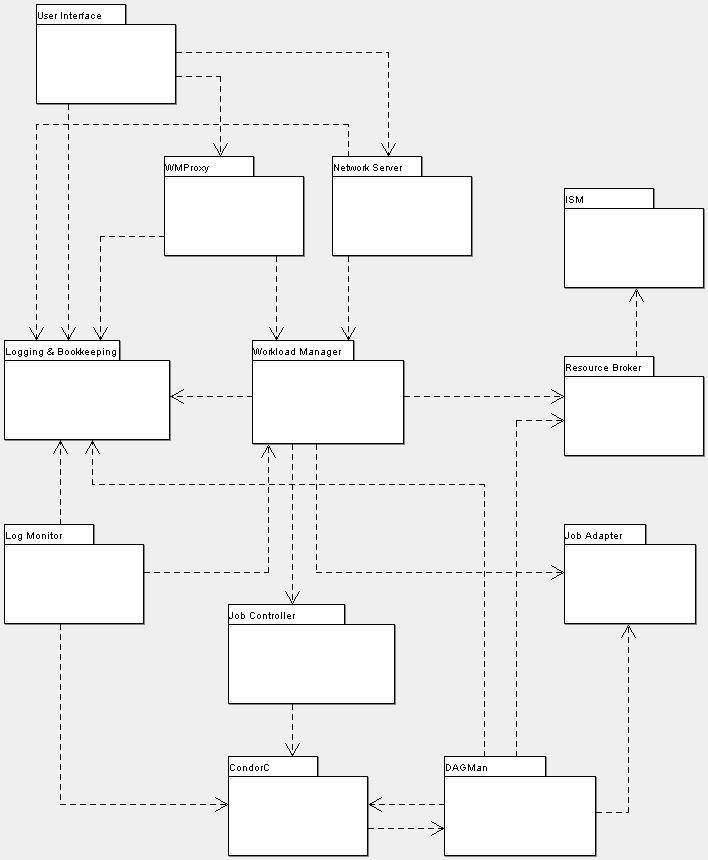
\includegraphics[width=0.92\hsize]{glite-wms}
%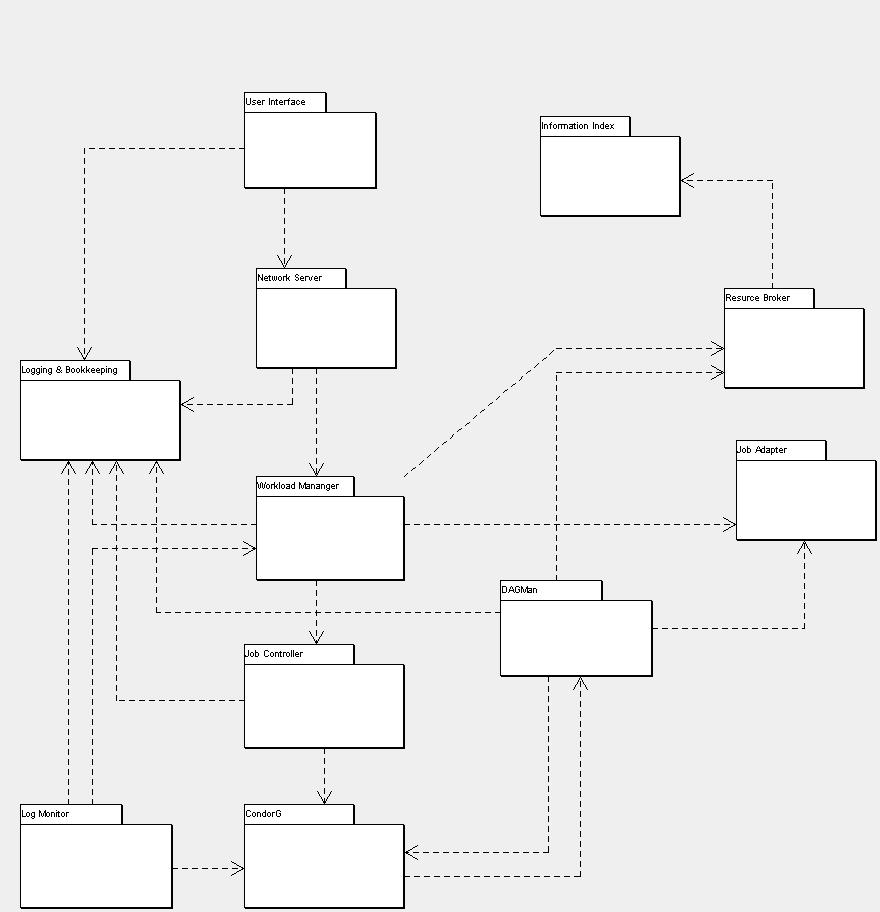
\includegraphics[width=1\hsize]{wp1-arch}
\caption{Overview of the WMS architecture}
\label{fig-arch}
\end{figure}


The {\bf Network Server} (NS) is a generic network daemon that provides support for the job control functionality. 
It is responsible for accepting incoming requests from the WMS-UI (e.g. job submission, job removal), which, if valid, 
are then passed to the Workload Manager.
\medskip

The {\bf Workload Manager Proxy} (WMProxy) is a service providing access to WMS functionality through a Web Services
based interface. Besides being the natural replacement of the NS in the passage to the SOA approach for the WMS 
architecture, it provides additional features such as bulk submission and the support for shared and compressed 
sandboxes for compound jobs. It can be accessed directly through the published WSDL available at 
\url{http://egee-jra1-wm.mi.infn.it/egee-jra1-wm/wmproxy} or using the provided client tools described in ~\cite{WMPROXY}. 

The {\bf Workload Manager} (WM) is the core component of the Workload Management System. Given a valid request, it 
has to take the appropriate actions to satisfy it. To do so, it may need support from other components, which are 
specific to the different request types.

For a computation job there are two main types of request: submission and cancellation. In particular the meaning 
of the submission request is to pass the responsibility of the job to the WM. The WM will then pass the job to an 
appropriate CE for execution, taking into account the requirements and the preferences expressed in the job 
description. The decision of which resource should be used is the outcome of a matchmaking process between the 
submission requests and the available resources. The availability of resources for a particular task depends not 
only on the state of the resources, but also on the utilisation policies that the resource administrators and/or 
the administrator of the VO the user belongs to have put in place.

The {\it Resource Broker} (RB) or Matchmaker is one of the "helper classes" offering support to the WM in 
taking the above mentioned decision. It provides a matchmaking service: given a JDL expression (e.g. for a 
job submission), it finds the resources that best match the request. 

A WM can adopt different policy in order to schedule a job. At one extreme a job is matched to a resource as 
soon as possible and, once the decision has been taken, the job is passed to the selected resource for execution. 
At the other extreme the jobs are held by the WM until a resource becomes available (eager scheduling), at which 
point that resource is matched against the submitted jobs and the job that fits best is passed to the resource 
for immediate execution (lazy scheduling policy). 

The mechanism that allows the flexible application of different policies is the decoupling between the collection 
of information concerning resources and its use.  
The {\it Information Super Market} (ISM) is the component that implements this mechanism and basically consists 
of a repository of resource information that is available in read only mode to the matchmaking engine and whose 
update is the result of either the arrival of notifications or active polling of resources or some arbitrary 
combination of both. Moreover the ISM can be configured so that certain notifications can trigger the matchmaking 
engine. These functionalities besides improving the modularity of the software also support the implementation of 
lazy scheduling policies.

The other fundamental component of the WM internal design is the {\it Task Queue (TQ)}, that gives the possibility 
to keep a submission request for a while if no resources are immediately available that match the job requirements. 
This technique is used, among others, by the AliEn and Condor systems. Non-matching requests will be 
retried either periodically (in an eager scheduling approach) or as soon as notifications of available resources 
appear in the ISM (in a lazy scheduling approach). Alternatively such situations could only lead to an immediate 
abort of the job for lack of a matching resource.
\medskip

Continuing with the WMS components handling the job during its lifetime, we have the {\bf Job Adapter} (JA) which 
is responsible for making the final touches to the JDL expression for a job, before it is passed to CondorC for the 
actual submission. So, besides preparing the CondorC submission file, this module is also responsible for creating 
the job wrapper script that creates the appropriate execution environment in the CE worker node (this includes the 
transfer of the input and of the output sandboxes).
\medskip

{\bf CondorC} is the module responsible for performing the actual job management operations (job submission, 
job removal, etc.), issued on request of the Workload Manager.
\medskip

{\bf DAGMan} (DAG Manager) is a meta-scheduler whose main purpose is to navigate the graph (i.e. the DAG request), 
determine which nodes are free of dependencies, and follow the execution of the corresponding jobs. A DAGMan 
instance is spawned by CondorC for each handled DAG. 

The {\bf Log Monitor} (LM) is responsible for watching the CondorC log file, intercepting interesting events 
concerning active jobs, that is events affecting the job state machine (e.g. job done, job canceled, etc.), and 
therefore triggering appropriate actions.

Moreover a {\bf Proxy Renewal Service} is available to assure that, for all the lifetime of a job, a valid user 
proxy exists within the WMS, and this proxy renewal service relies on the MyProxy service for renewing 
credentials associated to the request.
\medskip

The {\bf Logging and Bookkeeping} (LB) service provides support for the job monitoring functionality: it stores 
logging and bookkeeping information concerning events generated by the various components of the WMS. Using this 
information, the LB service keeps a state machine view of each job.
\medskip

The user can learn in which state its jobs are by querying the LB Service (using the appropriate command provided 
by the WMS-UI). Besides querying for the job state actively, the user may also register for receiving notifications on 
particular job state changes (e.g. when a job terminates). The notifications are delivered using an appropriate 
infrastructure.



\subsection{Interactions with other Services}
\label{interactions}
%\subsection{Interactions with other Services}

All WMS components described in section~\ref{arch} interact with the LB for logging information about the 
jobs they are handling and for querying information about them when needed.
Moreover during the matchmaking phase the Resource Broker interacts with the Data Management Catalogs through 
the StorageIndex interface to resolve the locations of existing file names specified in the JDL Inputdata list, 
so that the submitted job would run on worker node, close to the used files.

The WMS service also interacts with VOMS indirectly as it reads information about VO, groups and capabilities 
(Fully Qualified Attribute Names ~\cite{voms-core}) from the user's proxy credentials issued by VOMS to enforce 
user authentication and authorization.
The MyProxy service is contacted by the Proxy Renewal component of the WMS to renew automatically the 
credentials associated to long lived jobs.

Last but not least the WMS interacts with the CEs for submitting jobs (this goes through CondorC) and for receiving 
synchronous/asynchronous notifications about resource status and characteristics.
There could be configurations in which the WMS also interacts with the BDII to collect information about the whole 
resource pool available for a given VO. 




\subsection {Security} 
\label{security}
%\subsubsection {Security} 
 
For the Grid to be an effective framework for largely distributed computation, users, user processes 
and grid services must work in a secure environment.
 
Due to this, all interactions between WMS components, especially those that are network separated, will be 
mutually authenticated: depending on the specific interaction, an entity authenticates itself to the 
other peer using either its own credential or a delegated user credential or both. For example when the 
User Interface passes a job to the Network Server, the WMS-UI authenticates using a proxy user credential 
(a proxy certificate) whereas the NS uses its own service credential. The same happens when the WMS-UI 
interacts with the Logging and Bookkeeping service. The WMS-UI uses a proxy user credential to limit the risk 
of compromising the original credential in the hands of the user. 
 
The user or service identity and their public key are included in a X.509 certificate signed by a trusted 
Certification Authority (CA), whose purpose is to guarantee the association between that public key and its 
owner.

According to what just premised, to take advantage of WMS-UI commands the user has to possess a valid X.509 
certificate on the submitting machine, consisting of two files: the certificate file and the private 
key file. The location of the two mentioned files is assumed to be either pointed to respectively 
\textit{"\$X509\_USER\_CERT"} and \textit{"\$X509\_USER\_KEY"} or 
by \textit{"\$HOME\-/.globus\-/usercert.pem"} and \textit{"\$HOME\-/.globus/\-userkey.pem"} if the 
X509 environment variables are not set. 

\medskip


\framebox{
\parbox[c]{15cm}{
 
\textbf{How to extract userkey.pem and usercert.pem from your certificate}\medskip

Usually X.509 Certificates are downloaded using a browser and managed by the browser itself. 
Anyway it is possible to export your certificate in a file PKCS12 (which will probably have the 
extension .p12 or .pfx). 
 
The procedure to export the certificate vary from browser to browser, for example Internet Explorer 
starts with "Tools $->$ Internet Options $->$ Content"; Netscape Communicator has a "Security" button 
on the top menu bar; Mozilla starts with "Edit $->$ Preferences $->$ Privacy and Security $->$ Certificates" 
and Firefox has "Edit $->$ Preferences $->$ Advanced $->$ Certificates $->$ manage certificates $->$ backup".
  
Unfortunately PKCS12 format is not accepted by Globus security infrastructure, but you can easily convert 
it into the supported standard (PEM). This operation will split your *.p12 file in two files: the certificate 
(usercert.pm) and the private key (userkey.pm). The conversion can be performed with openssl tool:

\medskip

{\scriptsize{ 
\$ openssl pkcs12 -nocerts -in mycert.p12 -out userkey.pem\\
\$ openssl pkcs12 -clcerts -nokeys -in mycert.p12 -out usercert.pem\\
\$ chmod 0400 userkey.pem\\
\$ chmod 0600 usercert.pem\\
 }}
\medskip

Permission must be set as shown not only for security reasons: \emph{voms-proxy-init} and \emph{grid-proxy-init}
commands will fail if your private key is not protected as listed above.
}} 
%end of framebox and parbox
\medskip

Actually the user certificate and private key files are not mandatory on the WMS-UI machine; indeed they are 
only needed for the creation of the proxy user credentials through the \textit{grid-proxy-init} or 
\textit{voms-proxy-init} commands. Please refer to the VOMS User's Guide ~\cite{voms-core} for detailed 
information about the VOMS client commands.  

Alternatively you can download the proxy credentials from a trusted site and work with it without having 
the cert and key available locally.

All WMS-UI commands, when started, check for the existence and expiration date of a user proxy credentials in 
the location pointed to by \textit{"\$X509\_USER\_PROXY"} or in \textit{"/tmp/\-x509up\_u$<$UID$>$"} 
(where $<$UID$>$ is the user identifier in the submitting machine OS) if the X509 environment variable is 
not set. If the proxy certificate does not exist or has expired the WMS-UI returns an error message to the user 
and exits.

It is important to note that besides authentication, proxy credential issued by VOMS, i.e. containing 
FQANs (Fully Qualified Attribute Names ~\cite{voms-core}), are used by the WMS-UI to get the VO the user is currently working for. 
If a given proxy credential contains attributes for more then one VO, than the default one (i.e. the one first 
position) is considered.   

Once a job has been submitted by the WMS-UI, it passes through several components of the WMS 
(e.g. the NS, the WM, the JC, CondorC etc.) before it completes its execution. At each step operations 
that are related with the job could require authentication by a certificate. For example during the 
scheduling phase, the WM needs to get some information about the user who wants to schedule a job and 
the certificate of the user could be needed to access this information. Similarly, a valid user's certificate 
is needed by JC/CondorC to submit a job to the CE. Moreover JC has to be able to repeat this process e.g. 
in case of crashing of the CE which the job is running on, therefore, a valid user's certificate is needed 
for all the job lifetime.

A job gets associated a valid proxy certificate (the submitting user's one) when it is submitted by the WMS-UI to 
NS. Validity of such a certificate is set by default to 12 hours unless a longer validity is explicitly 
requested by the user when generating the proxy. Problems could occur if the job spends on CE (in a 
queue or running) more time than lifetime of its proxy certificate.

In order to submit long-running jobs, users can either generate proxy credentials using the respectively 
the \verb!--valid! and \verb!--hours! of the \textit{voms-proxy-init} and \textit{grid-proxy-init} commands 
or (more safely) rely on the features of the MyProxy package (see section~ref{myproxy}). The underlying idea 
is that the user registers in a MyProxy server a valid long-term certificate proxy that will be used by the 
WMS to perform a periodic credential renewal for the submitted job; in this way the user is no longer obliged 
to create very long lifetime proxies when submitting jobs lasting for a great amount of time. 
A more detailed description of this mechanism is provided in the following section~\ref{myproxy}.

\subsubsection {MyProxy} 
\label{myproxy}

The MyProxy credential repository system consists of a server and a set of client tools that can be used 
to delegate and retrieve credentials to and from a server. Normally, a user would start by using the 
\textit{myproxy\_init} client program along with the permanent credentials necessary to contact the server 
and delegate a set of proxy credentials to the server along with authentication information and retrieval 
restrictions.

\medskip
\textbf{MyProxy Client}
\medskip

The set of binaries provided for the client is made of the following files:

\begin{itemize}
\item \textit{myproxy-init}
\item \textit{myproxy-info}
\item \textit{myproxy-destroy}
\item \textit{myproxy-get-delegation}
\item \textit{myproxy-change-pass-phrase}
\end{itemize}


The {\bf myproxy-init} command allows you to create and send a delegated proxy to a MyProxy server for 
later retrieval; in order to launch it you have to assure you're able to execute the grid-proxy-init 
or voms-proxy-init command (i.e. the binary is visible from your \$PATH environment and the required 
cert files are either stored in the common path or specified with the X509 variables). You can use the 
command as follows (you will be asked for your PEM passhprase):

\smallskip
{\scriptsize{\verb!myproxy-init -s <host name> -t <hours> -d -n!}}
\smallskip

The myproxy-init command stores a user proxy in the repository specified by $<$host name$>$ (the -s option). 
Default lifetime of proxies retrieved from the repository will be set to $<$hours$>$  (see -t) and no 
password authorization is permitted when fetching the proxy from the repository (the  -n option). 
The proxy is stored under the same user-name as is your subject in your certificate (-d).

\medskip
The {\bf myproxy-info} command returns the remaining lifetime of the proxy in the repository along 
with subject name of the proxy owner (in our case it will be the same as in your proxy certificate). 
So if you want to get information about the stored proxies you can issue:

\smallskip
{\scriptsize{\verb!myproxy-info -s <host name> -d!}}
\smallskip

where -s and -d options have already been explained in the myproy-init command.

\medskip
The {\bf myproxy-destroy} command simply destroys any existing proxy stored in the myproxy server. 
You can use it as follows:

\smallskip
{\scriptsize{\verb!myproxy-destroy  -s <host name> -d!}}
\smallskip

where -s and -d options have already been explained in the myproy-init command

\medskip
The {\bf myproxy-get-delegation} command is indeed used to retrieve information about the proxies 
stored in the myproxy server. You can use it as follows:

\smallskip
{\scriptsize{\verb!myproxy-get-delegation -s <host name> -d -t <hours> -o <output file> -a <user proxy>!}}
\smallskip

You should end up with a retrieved proxy in $<$output file$>$, which is valid for
$<$hours$>$ hours.

It is worth noting that the environment variable MYPROXY\-\_SERVER can be set to tell to all these 
programs the hostname where the myproxy server is running.

\medskip
{\bf myproxy-change-pass-phrase}  

The  myproxy-change-pass-phrase  command  changes  the passphrase under which a credential is protected 
in the MyProxy repository.  The command first prompts for  the  current  passphrase  for the credential, 
then prompts twice for the new passphrase.  Only the  credential  owner  can change  a  credential's 
passphrase. 
The user must have a valid proxy credential as generated by grid-proxy-init or voms-proxy-init or retrieved 
by myproxy-get-delegation when running this command.
   
%}

 
\section{Quick-start Guide}
\label{quickstart}
%\section{Quickstart Guide}
% The quickstart guide should explain in simple terms and with examples
% how a user is supposed to achieve the most common usecases. E.g. how
% to submit and cancel a job, how to receive a job's output. How to
% create a grid file, move it around, locate it, and delete it. How to
% monitor the progress on an application etc.

This section briefly explains the sequence of operations, from the client configuration, to the description of the 
request up to the retrieval of the generated output, to be performed by a user to have his application run on a 
grid resource.
 

\subsection{Configuration}

Configuration of the WMS User Interface VO-specific parameters is accomplished through the file:

\smallskip
\begin{verbatim}
$GLITE_LOCATION/etc/<vo name>/glite_wmsui.conf 
\end{verbatim}
\smallskip

i.e. there is one directory and file for each supported VO.

If you wish to add a new VO among the ones supported by the WMS-UI, you must create a directory in \$GLITE\_LOCATION/etc, 
named as the VO (lower-case), copy in it the file: 

\smallskip
\begin{verbatim}
$GLITE_LOCATION/etc/vo_template/glite_wmsui.conf 
\end{verbatim}
\smallskip

distributed with the WMS-UI package and update it according to the given VO.

Here follows an example of WMS-UI configuration file for the "EGEE" Virtual Organisation. 
This implies that the file path has to be \emph{\$GLITE\_LOCATION/etc/egee/glite\_wmsui.conf}: 

\smallskip
\begin{verbatim}

[
 VirtualOrganisation = "EGEE";
 NSAddresses = {
   "tigerman.cnaf.infn.it:7772",
   "gundam.cnaf.infn.it:7772"
   };
 LBAddresses = {
   {"tigerman.cnaf.infn.it:9000", "fox.to.infn.it:9000"},
   {"gundam.cnaf.infn.it:9000", "neo.datamat.it:9000", "grid003.ct.infn.it:9876"}
  };
 MyProxyServer = "skurut.cesnet.cz";
 LoggingDestination = "localhost:9002";  // local instance of LB logging service
]

\end{verbatim}
\smallskip

This files indicates that there are two available Network Servers that can be contacted for the EGEE VO (they
are chosen randomly by the WMS-UI) and each NS has a group of associated LB servers:

\begin{itemize}
   \item tigerman.cnaf.infn.it:7772 is associated with tigerman.cnaf.infn.it:9000 and 
fox.to.infn.it:9000
   \item gundam.cnaf.infn.it:9000 is associated with gundam.cnaf.infn.it:9000, neo.datamat.it:9000 
and grid003.ct.infn.it:9876
\end{itemize}

Given a NS the WMS-UI chooses randomly the LB from the corresponding list. This feature can be used to
distribute load over several LB servers, although in most of cases there is a one-to-one correspondence
between NS and LB.

The \emph{MyProxyServer} parameter provides the host FQDN (fully qualified host name) of the MyProxy server 
to be used for proxy renewal (see \ref{longjob}) whilst \emph{LoggingDestination} has to be set in case of 
non-standard location of the LB locallogger (it usually runs on the WMS node). 

The other configuration file for the WMS-UI is

\smallskip
\begin{verbatim}
$GLITE_LOCATION/etc/glite_wmsui_cmd_var.conf
\end{verbatim}
\smallskip

The glite\_wmsui\_cmd\_var.conf file is a class-ad containing information that are not VO specific. 

\textbf{Example:}
\smallskip
\begin{verbatim}
[ 
 requirements = other.GlueCEStateStatus == "Production" ; 
 rank = - other.GlueCEStateEstimatedResponseTime ; 
 RetryCount = 3 ; 
 ErrorStorage= "/var/tmp" ; 
 OutputStorage="/tmp/jobOutput"; 
 ListenerStorage = "/tmp" 
 LoggingTimeout = 30 ; 
 LoggingSyncTimeout = 60 ;  
 DefaultStatusLevel = 1 ; 
 DefaultLogInfoLevel = 0; 
 NSLoggerLevel = 2; 
] 
\end{verbatim}
\smallskip

Details about configuration of the WMS-UI are provided in Section~\ref{cli}).

If you need to customise these files and you do not have root access on the WMS-UI machine, you can work with your own 
copies of them using the \emph{--config-vo} and \emph{--config} options of the WMS-UI commands.

\subsection{Environment Variables}

These are the environment variables that influence the behavior of the WMS-UI:

\begin{itemize}
 \item GLITE\_WMSUI\_CONFIG\_VAR Non-standard location of the command line interface configuration file 
   glite\_wmsui\_cmd\_var.conf. This variable points to the file absolute path
 \item GLITE\_WMSUI\_CONFIG\_VO  Non-standard location of the vo-specific GUI configuration file 
   glite\_wmsui.conf. This variable points to the file absolute path.
 \item EDG\_WL\_LOG\_DESTINATION Non-standard address of the the LB logging service (glite-lb-locallogger logging 
   daemon ~\cite{lb}) in the format $<$host FQDN$>$[:$<$port$>$]. If not set the LB logging service running on the WMS node is
   targeted for logging job information.
\end{itemize}


\subsection{Main commands}

The most relevant commands to interact with the WMS are:

\begin{itemize}
   \item glite-job-list-match $<$jdl\_file$>$
   \item glite-job-submit $<$jdl\_file$>$
   \item glite-job-status $<$job\_Id$>$
   \item glite-job-output $<$job\_Id$>$
   \item glite-job-cancel $<$job\_Id$>$
\end{itemize}

You can access information about the usage of each command by issuing either:

\smallskip
\begin{scriptsize}
\begin{verbatim}
> <command> --help
\end{verbatim}
\end{scriptsize}

\smallskip
or
\smallskip

\begin{scriptsize}
\begin{verbatim}
> man <command>
\end{verbatim}
\end{scriptsize}


\smallskip

\textbf{glite-job-list-match}

Displays the list of identifiers of the resources (and the corresponding ranks - if requested) on which the user 
is authorized and satisfying the job requirements included in the JDL. This only works for jobs; for DAGs you have to 
issue this commands on the single nodes JDLs. 

\textbf{glite-job-submit}

This command submits a job/DAG to the grid. It requires a JDL file as input and returns a job/DAG Identifier.

\textbf{glite-job-status}

This command prints the status of a job/DAG previously submitted using glite-job-submit. The job status request is sent 
to the LB (Logging and Bookkeeping service) that provides the requested information. 
When issued for a DAG it provides the status information for the DAG itself and all of its nodes. 
It is also possible to retrieve the status of individual nodes of a DAG simply passing their own identifiers to the 
command. \
The LB service  using the job/DAG related events sent by each WMS component handling the request, keeps a state machine 
view of each job/DAG. 

Figure~\ref{job-state} represents the job life-cycle state machine: 

\clearpage

\begin{figure}[htb]
\centering
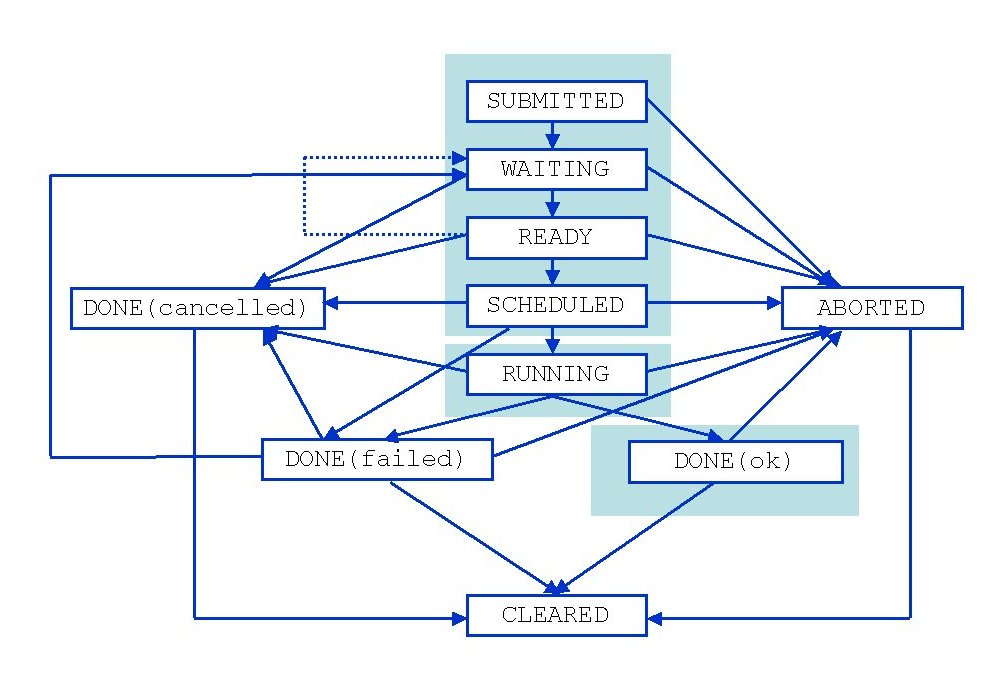
\includegraphics[width=.8\hsize]{job-state-diagram}
\caption{Job State Machine}
\label{job-state}
\end{figure}

Here below is provided a brief description of the meaning of each possible state a job/DAG can enter:

\begin{itemize}
\item {\it Submitted}: job is entered by the user to the User Interface but not yet transferred to Network Server for processing
\item {\it Waiting}: job has been accepted by NS and is waiting for Workload Manager processing or is being processed by WM Helper modules (e.g., WM is busy, no appropriate Computing Element (cluster) has been found yet, required dataset is not available, job is waiting for resource allocation).
\item {\it Ready}: job has been processed by WM and its Helper modules (especially, appropriate Computing Element has been found) but not yet transferred to the Computing Element (local batch system queue) via Job Controller and CondorC. This state does 
not exists for a DAG as it is not subjected to matchmaking (the nodes are) but passed directly to DAGMan.  
\item {\it Scheduled}: job is waiting in the queue on the Computing Element. This state also does not exists for a DAG as it is not directly sent to a CE (the node are). 
\item {\it Running}: job is running. For a DAG this means that DAGMan has started processing it.
\item {\it Done}: job exited or is considered to be in a terminal state by CondorC (e.g., submission to CE has failed in an unrecoverable way). 
\item {\it Aborted}: job processing was aborted by WMS (waiting in the Workload Manager queue or Computing Element for too long, over-use of quotas, expiration of user credentials, etc.).
\item {\it Canceled}: job has been successfully canceled on user request.
\item {\it Cleared}: output sandbox was transferred to the user or removed due to the timeout.
\end{itemize} 

Taken into account remarks about DAGs in the previous state description, the following figure~\ref{dag-state} represents instead the DAG 
life-cycle state machine:

\begin{figure}[htb]
\centering
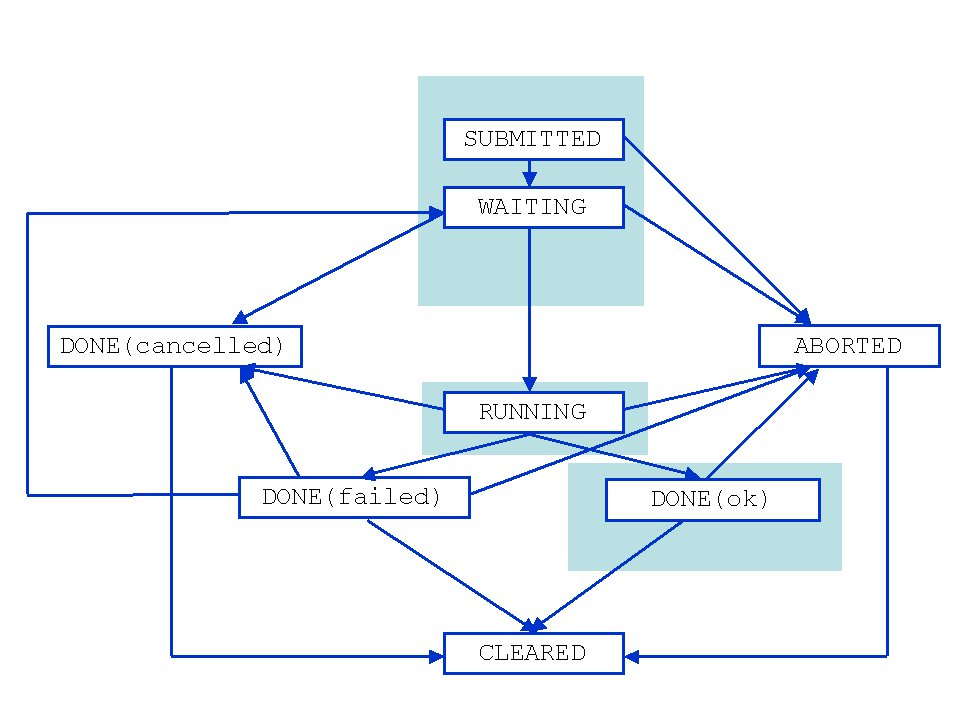
\includegraphics[width=.8\hsize]{dag-state-diagram}
\caption{DAG State Machine}
\label{dag-state}
\end{figure}

\newpage
 
\textbf{glite-job-output}

The glite-job-output command can be used to retrieve the output files of a job/DAG that has been submitted through the 
glite-job-submit command with a job description file including the OutputSandbox attribute. After the submission, 
when the job/DAG has terminated its execution, the user can download the files generated by the job/DAG and temporarily 
stored on the Resource Broker machine as specified by the OutputSandbox attribute, issuing the 
glite-job-output with as input the ID returned by the glite-job-submit. As a DAG does not have its own output sandbox, 
when the command is issues for such a request retrieves the output sandboxes of all the DAG nodes.

\textbf{glite-job-cancel}

This command cancels a job previously submitted using glite-job-submit. Before cancellation, it prompts the user 
for confirmation. The cancel request is sent to the Network Server that forwards it to the WM that fulfills it. 
It is not allowed to issue a cancel request for a node of a DAG: you have to cancel the whole DAG using the 
provided handle instead.


\medskip

The WMS-UI also provides three additional commands. They are: 

\begin{itemize}
   \item glite-job-logging-info $<$job\_Id$>$ (mostly useful for debugging purposes)
   \item glite-job-attach $<$job\_Id$>$ (for interactive jobs only)
   \item glite-job-get-chkpt $<$job\_Id$>$ (for checkpointable jobs only)
\end{itemize}


\textbf{glite-job-logging-info}

This command prints all the events related to a previously submitted job/DAG, that have been logged to the LB during 
request's lifetime by the WMS components that have handled it. The job/DAG logging-info request is sent
to the LB (Logging and Bookkeeping service) that provides the requested information. When issues for a DAG the 
command only displays events related to the DAG itself and not the ones of the nodes. 

\textbf{glite-job-attach}

This command attaches a listener to a previously submitted interactive job. This will make the job standard streams 
be re-directed to the command shell (or to a dedicated graphical window - if requested).

\textbf{glite-job-get-chkpt}

This command retrieves a checkpoint state of a a previously submitted checkpointable job. The retrieved state, that
is saved to a file on the WMS-UI machine, can be used later to re-submit either the same or another checkpointable 
job so that it will start its execution from the given state rather than from the beginning.

\smallskip
\subsection{The Job Identifier}

The Job (and DAG) Identifiers produced by the workload management software are of the form:

\smallskip
\begin{verbatim}
https://edt003.cnaf.infn.it:9000/NyIYrqE\_a8igk4f0CLXNKA
\end{verbatim}
\smallskip

The first part of the Id (\emph{https://edt003.cnaf.infn.it:9000} in the example above) is the endpoint URL of the 
LB server holding the job/DAG logging and bookkeeping information and this allows the WMS-UI to know which LB server has 
to be contacted for monitoring a given job/DAG. 
\smallskip
The second part (\emph{NyIYrqE\_a8igk4f0CLXNKA})  generated by the WMS-UI taking into account some client local information 
ensures instead grid-wide uniqueness of the identifier. 

    
\subsection{The Job Description File}

The key to the job submission and resource matching process is the JDL description file. This file describes 
the necessary inputs, generated outputs, and resource requirements of a job/DAG through the JDL 
(Job Description Language).

A typical example of a job description file is:

\smallskip
\begin{verbatim}
 [
   Type = "Job";
   JobType = "Normal";
   Executable = "myexe";
   StdInput = "myinput.txt";
   StdOutput = "message.txt";
   StdError = "error.txt";
   InputSandbox = {"/users/pacini/example/myinput.txt", 
                   "/users/pacini/example/myexe"};
   OutputSandbox = {"message.txt", "error.txt"};
   Requirements  = other.GlueCEInfoLRMSType == "PBS";
   Rank  = other.FreeCPUs;
 ]
\end{verbatim}
\smallskip

Such a JDL would make the \emph{myexe} executable be transferred on a remote CE whose queue is managed by the PBS batch 
system and be run taking the \emph{myinput.txt} file (also copied form the UI node) as input. The standard streams of the 
job are redirected on the worker node to file \emph{message.txt} and \emph{error.txt} and can be later retrieved on the 
WMS-UI by means of the \emph{glite-job-output} command. 


A simple example of DAG description, call it \emph{dag.jdl}, is instead:

\smallskip
\begin{verbatim}
 [
    Type = "dag";
    max_nodes_running = 10;
    VirtualOrganisation = "EGEE";
    nodes = [
      nodeA = [
        file ="/users/pacini/n1.jdl" ; 
      ];
      nodeB = [
        file ="/users/pacini/n2.jdl" ; 
      ];
      nodeB = [
        file ="/users/pacini/n3.jdl" ; 
      ];
      dependencies = {
        { nodeA, {nodeB, nodeC}}
      }
    ];
  ]
\end{verbatim}
\smallskip

where n1.jdl, n2.jdl and n3.jdl are in turn job descriptions representing the nodes of the DAG and the dependencies 
attributes states that \textit{nodeB} and \textit{nodeC} cannot start before \textit{nodeA} has been successfully executed. 
Also the DAGs are submitted through the \emph{glite-job-submit} command.

A detailed description of the available JDL attributes and of the rules for building correct JDL files is 
provided by the "JDL Attributes Specification" document ~\cite{jdl}.  

It is important to note note that the input and output sandboxes are intended for relatively small files 
(few megabytes) like scripts, standard input, and standard output streams.
If you are using large input files or generating large output files, you should instead directly read from or 
write to a storage element. As each submitting user is assigned by the WMS with a limited quota on the WMS 
machine disk, abuse of the input and output sandboxes will shortly make the quota fill-up and the WMS not accept 
further jobs submission for the given user. 

The parameters Requirements and Rank control the resource matching for the job. The expression given for the 
requirements specifies the constraints necessary for a job to run. In the example above, a site running PBS is 
required and the job will only be submitted to resources which satisfy this condition. If more than one resource 
matches the job requirements, then the rank is used to determine which is the most desirable resource i.e. the one 
to which the job is submitted (the higher the rank value the better is the resource). 
Both, the Requirements and the rank attributes, can be arbitrary expressions which use the parameters published 
by the resources in the Information System or directly to the ISM.
A DAG does not have its own requirements and ranking expressions: matchmaking is performed on the individual nodes 
Rank and Requirements.

\smallskip
\subsection{Commands Sequence}

This section reports an example of the sequence of steps that have to be performed to do a job submission and to monitor 
the submitted job.
 
Before using any of the WMS-UI commands it is necessary to have a valid proxy credential available on the WMS-UI
machine. You can create it using the \textit{voms-proxy-init} command or alternatively the \textit{grid-proxy-init} one. 
If you already have a valid proxy available on your machine just make the X509\_USER\_PROXY environment variable 
point to it.

In order to get a proxy certificates issued by VOMS ~\cite{voms-core} you should have in your home directory the file 
\$HOME/.glite/vomses containing a line as follows:

\smallskip
{\scriptsize{\verb!"EGEE" "kuiken.nikhef.nl" "15001" "/O=dutchgrid/O=hosts/OU=nikhef.nl/CN=kuiken.nikhef.nl" "EGEE" "22"!}}
\smallskip

or the corresponding line for your VO (ask your VO admin for that).


Make moreover sure you have in the directory \textit{\$HOME/.globus} your certificate/key pair, i.e. the following files:  

\smallskip

\begin{scriptsize}
\begin{verbatim}
usercert.pem
userkey.pem
\end{verbatim}
\end{scriptsize}
\smallskip

Note that file permissions are important: the two files must have respectively \textit{0600} and \textit{0400} permissions.  

Then you can issue the VOMS client command (you will be prompted for the pass-phrase):

\smallskip
\begin{scriptsize}
\begin{verbatim}

> voms-proxy-init --userconf vomses -voms EGEE
Your identity: /C=IT/O=INFN/OU=Personal Certificate/L=DATAMAT DSAGRD/CN=Fabrizio Pacini
Enter GRID pass phrase for this identity:
Creating temporary proxy ..................................... Done
/O=dutchgrid/O=hosts/OU=nikhef.nl/CN=kuiken.nikhef.nl
/C=NL/O=NIKHEF/CN=NIKHEF medium-security certification auth
Creating proxy ............................ Done
Your proxy is valid until Sat Mar  5 06:13:07 2005

> voms-proxy-info
VO              : EGEE
Valid from      : Mar  4 17:13:08 2005 GMT
Valid to        : Mar  5 05:13:08 2005 GMT

\end{verbatim}
\end{scriptsize}
\smallskip


Now you can start using the WMS-UI commands.
It is often useful to check the results of the resource matching before submitting a job. For this, one can use 
the \emph{glite-job-list-match} command. Given the JDL file it will return a ranked list of matching resources. 
The highest-ranked resource will appear first.

Take for example the following  JDL file, say \textit{ HelloWorld.jdl}:

\smallskip
\begin{verbatim}

 [
   Executable = "/bin/echo";
   Arguments = "Hello World";
   StdOutput = "message.txt";   StdError = "stderror";
   OutputSandbox = {"message.txt","stderror"};
   rank = -other.GlueCEStateEstimatedResponseTime;
   requirements = other.GlueCEStateStatus == "Production"; 
 ]

\end{verbatim}
\smallskip

you can get the list of available CEids and then submit as follows: 

\smallskip
\begin{scriptsize}
\begin{verbatim}

> glite-job-list-match HelloWorld.jdl
   
Selected Virtual Organisation name (from proxy certificate extension): EGEE   
Connecting to host edt003.cnaf.infn.it, port 7772

****************************************************
                    COMPUTING ELEMENT IDs LIST
The following CE(s) matching your job requirements 
have been found:

                            *CEId*
grid20.bo.ingv.it:2119/jobmanager-pbs-infinite
grid20.bo.ingv.it:2119/jobmanager-pbs-long
grid20.bo.ingv.it:2119/jobmanager-pbs-short
gridba2.ba.infn.it:2119/jobmanager-lcgpbs-infinite
gridba2.ba.infn.it:2119/jobmanager-lcgpbs-long
gridba2.ba.infn.it:2119/jobmanager-lcgpbs-short
gridit001.pd.infn.it:2119/jobmanager-pbs-infinite
gridit001.pd.infn.it:2119/jobmanager-pbs-long
gridit001.pd.infn.it:2119/jobmanager-pbs-short
****************************************************

\end{verbatim}
\end{scriptsize}
\smallskip

and once verified that you are happy with the matching resources, you cab actually submit the job:

\smallskip
\begin{scriptsize}
\begin{verbatim}

> glite-job-submit HelloWorld.jdl

Selected Virtual Organisation name (from proxy certificate extension): EGEE
Connecting to host edt003.cnaf.infn.it, port 7772
Logging to host edt003.cnaf.infn.it, port 9002

**************************************************************
                  JOB SUBMIT OUTCOME
The job has been successfully submitted to the Network Server.
Use glite-job-status command to check job current status. 
Your job identifier is:

- https://edt003.cnaf.infn.it:9000/NyIYrqE\_a8igk4f0CLXNKA

***************************************************************

\end{verbatim}
\end{scriptsize}
\smallskip


Note that this command returns the job identifier associated with this job. The job Id 
is the unique Grid Job Identifier, assigned from the WMS (Workload Management System) to every job in order to 
be able to identify it in clear and unique way all over the Grid system scope.

Passing the job id handle to the WMS commands you can follow-up the submitted job:

\smallskip
\begin{scriptsize}
\begin{verbatim}

> glite-job-status https://edt003.cnaf.infn.it:9000/NyIYrqE\_a8igk4f0CLXNKA

****************************************************************************
BOOKKEEPING INFORMATION:

Printing status info for the Job :
https://edt003.cnaf.infn.it:9000/NyIYrqE\_a8igk4f0CLXNKA
Current Status:Done (Success)
Exit code: 0
Status Reason: Job terminated successfully
Destination:   gridit001.pd.infn.it:2119/jobmanager-lcgpbs-infinite
reached on:Mon Sep 22 09:37:13 2003 CET
****************************************************************************
\end{verbatim}
\end{scriptsize}
\smallskip

States seen in the normal processing of jobs are: \textit{Submitted, Waiting, Ready, Running} and \textit{Done}. Abnormal 
execution usually ends with an Aborted status.

Once you have checked that the job has terminated its execution successfully (\emph{Done} status), i.e. the job has 
finished and the output has been pushed back to the WMS node, you can retrieve the output of your job to the 
WMS-UI machine as follows:

\smallskip
\begin{scriptsize}
\begin{verbatim}

> glite-job-output https://edt003.cnaf.infn.it:9000/NyIYrqE\_a8igk4f0CLXNKA

Retrieving files from host edt003.cnaf.infn.it

****************************************************************************
		JOB GET OUTPUT OUTCOME

Output sandbox files for the job:
- https://edt003.cnaf.infn.it:9000/NyIYrqE\_a8igk4f0CLXNKA
have been successfully retrieved and stored in the directory:
/tmp/jobOutput/mrossi__NyIYrqE\_a8igk4f0CLXNKA

****************************************************************************
\end{verbatim}
\end{scriptsize}
\smallskip

where \textit{/tmp/jobOutput} is the output storage path set in you configuration file and 
\textit{mrossi\_\_NyIYrqE\_a8igk4f0CLXNKA} is a directory name built concatenating your current OS user-name and
the job Id unique string. 

Use the \emph{--dir} option if you want the output to be saved in a location different from \textit{/tmp/jobOutput}.  

Handling the job identifiers directly quickly becomes tedious. To avoid this, you can make the \emph{glite-job-submit} 
command append the job Id to a named file using the \emph{--output} option. 
On the other side, the WMS-UI commands which take job identifiers as an argument accept also the \emph{--input} option 
which allows the job identifier to be read from a file.
It is possible anyway to retrieve the status information for all jobs you have submitted  for a given VO by using 
the \emph{--all} option of the  \emph{glite-job-status} command: 

\smallskip
\begin{scriptsize}
\begin{verbatim}

> glite-job-status --all 

\end{verbatim}
\end{scriptsize}
\smallskip


If something is not going as expected with your job, e.g. it is \textit{Aborted} or it does not reach the \textit{Done} 
status you can try the \emph{glite-job-logging-info} command to inspect the job related events. Assuming your job 
identifier is e.g. \textit{https://gundam.cnaf.infn.it:9000/WkyitIdNTR0C9adOcBPhwg}, you can type:

\smallskip
\begin{scriptsize}
\begin{verbatim}

> glite-job-logging-info https://gundam.cnaf.infn.it:9000/WkyitIdNTR0C9adOcBPhwg

**********************************************************************
LOGGING INFORMATION:

Printing info for the Job : https://gundam.cnaf.infn.it:9000/WkyitIdNTR0C9adOcBPhwg
 
        ---
Event: RegJob
- source                  =    UserInterface
- timestamp               =    Fri Mar  4 18:05:28 2005 CET
        ---
Event: Transfer
- destination             =    NetworkServer
- result                  =    START
- source                  =    UserInterface
- timestamp               =    Fri Mar  4 18:05:29 2005 CET
        ---
Event: Transfer
- destination             =    NetworkServer
- result                  =    OK
- source                  =    UserInterface
- timestamp               =    Fri Mar  4 18:05:32 2005 CET
        ---
Event: Accepted
- source                  =    NetworkServer
- timestamp               =    Fri Mar  4 18:05:23 2005 CET
        ---
....

\end{verbatim}
\end{scriptsize}
\smallskip

to check if there was a problem within a certain WMS component and eventually cancel it with :

\smallskip
\begin{scriptsize}
\begin{verbatim}

> glite-job-cancel https://gundam.cnaf.infn.it:9000/SpLbPbMpftBSnCr0WwJmZA

Are you sure you want to remove specified job(s)? [y/n]n :y

=============================  glite-job-cancel Success  ===========================
 The cancellation request has been successfully submitted for the following job(s):

 - https://gundam.cnaf.infn.it:9000/SpLbPbMpftBSnCr0WwJmZA

====================================================================================

\end{verbatim}
\end{scriptsize}
\smallskip

\subsubsection {DAGs}

DAG submission can be accomplished through the same commands used for simple jobs. 
If for example you want to submit the DAG defined above, \emph{dag.jdl}, once you have 
completed the proxy preparation steps, just issue the following command: 

\smallskip
\begin{scriptsize}
\begin{verbatim}

> glite-job-submit dag.jdl 

Selected Virtual Organisation name (from proxy certificate extension): EGEE
Connecting to host gundam.cnaf.infn.it, port 7772
Logging to host gundam.cnaf.infn.it, port 9002


**************************************************************************************
                               JOB SUBMIT OUTCOME
 The dag has been successfully submitted to the Network Server.
 Use glite-job-status command to check job current status. Your dag identifier is:

 - https://gundam.cnaf.infn.it:9000/AhM4clHKVD1VMOMVrdkCZw


**************************************************************************************
\end{verbatim}
\end{scriptsize}


and then monitor it by means of:


\smallskip
\begin{scriptsize}
\begin{verbatim}

> glite-job-status https://gundam.cnaf.infn.it:9000/AhM4clHKVD1VMOMVrdkCZw


*************************************************************
BOOKKEEPING INFORMATION:

Status info for the Job : https://gundam.cnaf.infn.it:9000/AhM4clHKVD1VMOMVrdkCZw
Current Status:     Ready 
Status Reason:      unavailable
Destination:        dagman
Submitted:          Mon Mar  7 17:25:22 2005 CET
*************************************************************

- Nodes information for: 
    Status info for the Job : https://gundam.cnaf.infn.it:9000/ayNofwCnlusD68s3qQvFEA
    Current Status:     Submitted 
    Submitted:          Mon Mar  7 17:25:08 2005 CET
    Parent Job:         https://gundam.cnaf.infn.it:9000/AhM4clHKVD1VMOMVrdkCZw
*************************************************************
    
    Status info for the Job : https://gundam.cnaf.infn.it:9000/9FfFXd7UIWuoPSlyqMVZNQ
    Current Status:     Submitted 
    Submitted:          Mon Mar  7 17:25:08 2005 CET
    Parent Job:         https://gundam.cnaf.infn.it:9000/AhM4clHKVD1VMOMVrdkCZw
*************************************************************
    
    Status info for the Job : https://gundam.cnaf.infn.it:9000/wlgiicvWUe6Br7nbjIxcnQ
    Current Status:     Submitted 
    Submitted:          Mon Mar  7 17:25:08 2005 CET
    Parent Job:         https://gundam.cnaf.infn.it:9000/AhM4clHKVD1VMOMVrdkCZw
*************************************************************

\end{verbatim}
\end{scriptsize}
\smallskip

As you can see the \emph{glite-job-status} command shows in this case information about the DAG
itself and all its nodes. Nodes can be also followed-up singularly by picking their job identifiers.

The \emph{glite-job-logging-info} returns instead only the events related to the DAG. Nodes logging information
have to be requested explicitly specifying the node Id. 

The \emph{glite-job-output} can be used for a DAG to request the retrieval of the output sandboxes of all its nodes. 

The \emph{glite-job-cancel} commands can be used for a DAG to request cancellation of the whole DAG whilst cannot be 
called for a single DAG node.  


\subsection {Long Lived Jobs}
\label{longjob}

It is possible that long jobs may outlive the validity of the initial proxy; if so and the proxy 
is not renewed, the job will die prematurely. To avoid this the workload management software allows 
the proxy to be renewed automatically if your credentials are managed by a MyProxy server.

To use the automatic proxy renewal mechanism, first register a proxy with the MyProxy server using 
the command

\smallskip
\verb!myproxy-init -s <server> -t <hours>  -d -n!
\smallskip

where \emph{server} is the MyProxy server address, \emph{hours} is the number of hours the proxy should be valid on the 
server.

As this proxy is only copied to the server, you will need to create a local short-lived proxy using 
voms-proxy-init as explained previously, to do the job submissions. The Workload Manager will 
retrieve renewed proxies from the MyProxy server for jobs which need and request them. 
The need for proxy renewal has to be explicitly specified in the JDL of the job/DAG through the 
\emph{MyProxyServer} attribute, e.g.:

\smallskip
\begin{verbatim}
MyProxyServer = "skurut.ics.muni.cz";
\end{verbatim}
\smallskip


Information about your stored proxy can be obtained via the command

\smallskip
\verb!myproxy-info -s <server> -d!
\smallskip

and the proxy can be removed with

\smallskip
\verb!myproxy-destroy -s <server> -d.!
\smallskip

Once the proxy is removed from the server, running jobs will no longer receive renewed credentials.


\subsection{Specifying Job Requirements}

By specifying job requirements, the user can steer the job to sites which have the resources 
necessary to run the job correctly. Incompletely specifying the requirements may cause the job 
to fail, wasting both the resources and the user's time.

The request requirements are specified through the \emph{Requirements} attribute in the JDL 
description of the job. The value of this attribute is a boolean expression which specifies the 
necessary constraints. Nearly the full set of C operators and syntax are supported.

The values (or variables) which can be used in the requirements expression can be found by looking 
at the Computing Element attributes in the BDII or subscribing to the CE Monitor notification service.
The current Glue Schema used for publishing CE information is however available at:
\url{http://www.cnaf.infn.it/~sergio/datatag/glue/index.htm}. Most of the attributes are 
self-explanatory.

For example to express that a job requires at least 25 minutes of CPU time and 100 minutes of real 
time, the expression:

\smallskip
{\scriptsize{
\verb!Requirements = other.GlueCEPolicyMaxCPUTime >= 1500 && other.GlueCEPolicyMaxWallClockTime >= 6000;!
}}
\smallskip


would limit the matching to viable sites. The times are given in seconds. 
Note that the attribute names are prefixed with \textit{other.}; this is a remnant of the Class-Ads syntax on 
which JDL is based indicating the the prefixed attribute has to be searched in the counterpart class-ad (i.e. the 
one describing the resource). Note also that the values are not quoted. Using quotes around a numeric value 
will result in a string comparison which will produce an erroneous match (or none at all).

The \textit{GlueHostApplicationSoftwareRunTimeEnvironment} is usually used to describe application software 
packages which are installed on a site. For example:

\smallskip
{\scriptsize{
\verb!Requirements  = Member(other.GlueHostApplicationSoftwareRunTimeEnvironment ,"ALICE-3.07.01");!
}}
\smallskip

will choose a site with the ALICE-3.07.01 tag defined. The \textit{GlueHostApplicationSoftwareRunTimeEnvironment} 
is a multi-valued attribute and evaluates to a list. The class-ad \textit{Member} function returns true if the given 
value is in the list.

The available built-in class-ad functions that can be used for building the requirements expression are 
described in ~\cite{jdl-lang}.

Occasionally, one may wish to exclude or include a site manually. Forcing a job to a site can be 
accomplished with the \emph{--resource} option of the glite-job-submit command. However, this 
entirely bypasses the matchmaking process and will not produce the \emph{.BrokerInfo} file, i.e. the 
file generated during the matchmaking phase, that is sent on the WN and contains data location 
information that can be useful for the job at run time. You can use instead a clause like:

\smallskip
{\scriptsize{
\verb!Requirements = other.GlueCEUniqueID == "ccgridli03.in2p3.fr:2119/jobmanager-bqs-A";!
}}
\smallskip
  
to do the same thing. More interestingly one can select or exclude a site:

\smallskip
\begin{scriptsize}
\begin{verbatim}   
Requirements  = RegExp(".*nikhef.*",other.GlueCEUniqueID);
Requirements  = (!(RegExp(".*nikhef.*",other.GlueCEUniqueID)));
\end{verbatim}
\end{scriptsize}
\smallskip


which cannot be accomplished with the --resource option. Note that the JDL is very picky about the 
logical not syntax. 

In the WMS-UI configuration file (\$GLITE\_LOCATION/etc/glite\_wmsui\_cmd\_var.conf) there is a 
requirements clause which is added to all JDL files by default. This is 

\smallskip
\begin{scriptsize}
\begin{verbatim}   
other.GlueCEStateStatus == "Production" ;
\end{verbatim}
\end{scriptsize}
\smallskip

If you have provided an expression for the requirements attribute in the JDL, the one specified in 
the configuration file is added (in AND) to the existing one. 

As a DAG does not have its own requirements, what stated in this section applies to the DAG nodes descriptions. 



\subsection{Ranking Resources}

If more than one resource matches the specified requirements, then the highest-ranked resource will
be used. If the Rank attribute is not specified in the user's JDL description, then

\smallskip
\begin{scriptsize}
\verb!Rank = - other.GlueCEStateEstimatedResponseTime ;!
\end{scriptsize}
\smallskip

is added by default by the WMS-UI (as specified in the WMS-UI configuration file).The traversal time is 
the expected time in seconds that a job will take to begin executing at the site from the it has 
entered the batch system queue.

This ranking is not always ideal, and the user may wish to choose some other criteria for the 
ranking. For example,

\smallskip
\begin{scriptsize}
\verb!Rank = other.GlueCEStateFreeCPUs ;!
\end{scriptsize}
\smallskip

will make the WMS choose the site with the largest number of free CPUs. The rule to remember is that 
the larger the rank, the more desirable the resource is. If more than one site has exactly the same 
rank, then the one which is used is chosen randomly by the RB.

As a DAG does not have its own rank, what stated in this section applies to the DAG nodes descriptions. 


\newpage
\section{Reference Guide}
\label{refguide}

%The reference guide should contain detailed descriptions of all
%provided CLIs and APIs. There should be two subsections for those.

\subsection{Command-Line Interfaces}
\label{cli}
%\subsection{Commandline Interfaces}

In this section we describe syntax and behavior of the commands made available by the WMS-UI to allow job/DAG 
submission, monitoring and control. In the commands synopsis the mandatory arguments are showed between 
angle brackets $<$arg$>$) whilst the optional ones between square brackets ([arg]).

Commands for accessing the WMS through the WMProxy service are described in document ~\cite{WMPROXY}.
Note that usage of the WMProxy submission and control client commands is strongly recommended as they 
provide full support for all new functionality and enhancements of the WMS. 

Before going to the single commands let's have a look at how the WMS-UI can be configured.


\medskip
\subsubsection{Commands Configuration}
\label{config}

\textbf{VO-Specific}

Configuration of the WMS User Interface VO-specific parameters is accomplished through the file:

\smallskip
\begin{verbatim}
$GLITE_LOCATION/etc/<vo name>/glite_wmsui.conf 
\end{verbatim}
\smallskip


i.e. there is one directory and file for each supported VO. 

The common WMS-UI configuration rpm (\textit{glite-wms-ui-configuration}) installs the following example file:

\smallskip
\begin{verbatim}
$GLITE_LOCATION/etc/vo_template/glite_wmsui.conf
\end{verbatim}
\smallskip

If the configuration for your VO is not present on the WMS-UI machine you must create in \$GLITE\_LOCATION/etc a 
directory, named as the VO (lower-case), copy in it the above mentioned template file and update it opportunely.

The \emph{glite\_wmsui.conf} file is a classad containing the following fields:

\smallskip

\begin{itemize}
 \item \textbf{VirtualOrganisation} this is a string representing the name of the virtual organisation the file refers to.
   It should match with the name of the directory containing the file (i.e. the VO). This parameter is 
   mandatory. 
 \item \textbf{NSAddresses} this is a list of strings representing the addresses ($<$hostname$>$:$<$port$>$) of the Network 
   Servers available for the given VO. Job submission is performed towards the NS picked-up randomly from 
   the list and in case of failure it is retried on each other listed NS until succes or the end of the 
   list is reached. This parameter is mandatory.
 \item \textbf{LBAddresses} this is a list of strings or a list of lists of strings representing the address or list 
   of addresses ($<$hostname$>$:$<$port$>$) of the LB servers available for the given VO for the corresponding NS. 
   I.e. the first list of LB addresses correspond to the first NS in the NSAddresses list, the second list 
   of LB addresses correspond to the second NS in the NSAddresses list and so on.
   When job submission is performed, the WMS-UI after having chosen the NS, choses randomly one LB server within
   the corresponding list and uses it for generating the job identifier so that all information related with 
   that job will be managed by the chosen LB server. This allows distributing load on several LB servers.  
   This parameter is mandatory.
 \item \textbf{HLRLocation} this is a string representing the address ($<$hostname$>$:$<$port$>$:$<$X509contact string$>$)  of the 
   HLR for the given VO. HLR is the service responsible for managing the economic transactions and the 
   accounts of user and resources. This parameter is not mandatory. It is not present in the file by default.
   If present, it makes the WMS-UI automatically add to the job description the HLRLocation JDL attribute 
   (if not specified by the user) and this enables accounting.
 \item \textbf{MyProxyServer} this is a string representing the MYProxy server address ($<$hostname$>$) for the given VO. 
   This parameter is not mandatory. It is not present in the file by default. If present, it makes the WMS-UI 
   automatically add to the job description the MyProxyServer JDL attribute (if not specified by the user) 
   and this enables proxy renewal. If the myproxy client package is installed on the WMS-UI node, then this 
   parameter should be set equal to the MYPROXY\_SERVER environment variable.
 \item \textbf{LoggingDestination} this is a string defining the address ($<$host$>$:$[<$port$>]$;) of the LB logging service 
   (glite-lb-locallogger logging daemon ) to be targeted when logging events. The WMS-UI first checks the 
   environment for the EDG\_WL\_LOG\_DESTINATION variable and only if this is not set, the value of the 
   LoggingDestination parameter is taken into account. Otherwise the job related events are logged to the 
   LB logging service running on the WMS node.

\end{itemize}
\smallskip

Here below is provided an example of configuration file for the "atlas" Virtual Organisation. 
This implies that the file path has to be \textit{\$GLITE\_LOCATION/etc/atlas/glite\_wmsui.conf}. 

\smallskip
\begin{verbatim}

[
 VirtualOrganisation = "atlas";
 NSAddresses = {
   "ibm139.cnaf.infn.it:7772",
   "gundam.cnaf.infn.it:7772"
   };
 LBAddresses = {
   {"ibm139.cnaf.infn.it:9000"},
   {"gundam.cnaf.infn.it:9000", "neo.datamat.it:9000", "grid003.ct.infn.it:9876"}
  };
 HLRLocation = "lilith.to.infn.it:56568:/C=IT/O=INFN/OU=Personal Certificate/L=Torino/CN=Andrea 
                Guarise/Email=A.Guarise@to.infn.it";
 MyProxyServer = "skurut.cesnet.cz";
 LoggingDestination = "localhost:9002";  // local instance of LB logging service
]

\end{verbatim}
\medskip
\medskip


\textbf{Generic}


Configuration of the WMS User Interface generic parameters is accomplished through the file:

\smallskip
\begin{verbatim}
$GLITE_LOCATION/etc/glite_wmsui_cmd_var.conf
\end{verbatim}
\smallskip


Update the content of the latter file according to your needs.

The \textit{glite\_wmsui\_cmd\_var.conf} file is a classad containing the following fields:


\smallskip

\begin{itemize}
 \item \textbf{requirements} this is an expression representing the default value for the requirements expression 
   in the JDL job description. This parameter is mandatory. The value of this parameter is assigned by 
   the WMS-UI to the requirements attribute in the JDL if not specified by the user. If the user has instead 
   provided an expression for the requirements attribute in the JDL, the one specified in the configuration 
   file is added (in AND) to the existing one. 
   E.g. if in the glite\_wmsui\_cmd\_var.conf configuration file there is: 

   \begin{scriptsize}   
   \textit{requirements = other.GlueCEStateStatus == "Production" ;} 
   \end{scriptsize}

   and in the JDL file the user has specified: 

   \begin{scriptsize}   
   \textit{requirements = other.GlueCEInfoLRMSType == "PBS";} 
   \end{scriptsize}

   then the job description that is passed to the WMS contains 

   \begin{scriptsize}   
   \textit{requirements = (other.GlueCEInfoLRMSType == "PBS") \&\& (other.GlueCEStateStatus == "Production");} 
   \end{scriptsize}
      
   Obviously the setting TRUE for the requirements in the configuration file does not have any impact on the evaluation 
   of job requirements as it would result in: 

   \begin{scriptsize}   
   \textit{requirements = (other.GlueCEInfoLRMSType == "PBS") \&\& TRUE ;}
   \end{scriptsize}

 \item \textbf{rank} this is an expression representing the default value for the rank expression in the JDL job 
   description. The value of this parameter is assigned by the WMS-UI to the rank attribute in the JDL if not 
   specified by the user. This parameter is mandatory.   
 \item \textbf{RetryCount} this is an integer representing the default value for the number of submission retries for 
   a job upon failure due to some grid component (i.e. not to the job itself). The value of this parameter 
   is assigned by the WMS-UI to the RetryCount attribute in the JDL if not specified by the user.   
 \item \textbf{DefaultVo} this is a string representing the name of the virtual organisation to be taken as the user s 
   VO (VirtualOrganisation attribute in he JDL) if not specified by the user neither in the credentials 
   VOMS extension, nor directly in the job description nor through the --vo option. This attribute can be 
   either set to  unspecified  or not included at all in the file to mean that no default is set for the VO. 
 \item \textbf{ErrorStorage} this is a string representing the path of the directory where the WMS-UI creates log files. 
   This directory is not created by the WMS-UI, so It has to be an already existing directory. Default for this 
   parameter is /tmp.   
 \item \textbf{OutputStorage} this is a string defining the path of the directory where the job OutputSandbox files are 
   stored if not specified by the user through commands options. This directory is not created by the WMS-UI, 
   so It has to be an already existing directory. Default for this parameter is /tmp. 
 \item \textbf{ListenerStorage} this is a string defining the path of the directory where are created the pipes where 
   the glite\_wms\_console\_shadow process saves the job standard streams for interactive jobs. Default for 
   this parameter is /tmp.   
 \item \textbf{LoggingTimeout} this is an integer representing the timeout in seconds for asynchronous logging function 
   called by the WMS-UI when logging events to the LB. Recommended value for WMS-UI that are non-local to the 
   logging service (glite-lb-logd logging daemon) is not less than 30 seconds. 
 \item \textbf{LoggingSyncTimeout} this is an integer representing the timeout in seconds for synchronous logging function
   called by the WMS-UI when logging events to the LB. Recommended value is not less than 30 seconds.   
 \item \textbf{DefaulStatusLevel} this is an integer defining the default level of verbosity for the glite-job-status 
   command. Possible values are 0,1,2 and 3. 1 is the default.
 \item \textbf{DefaultLogInfoLevel} this is an integer defining the default level of verbosity for the glite-job-logging-info
   command. Possible values are 0,1,2 and 3. 1 is the default. 
   Default for this parameter is 0.   
 \item \textbf{NSLoggerLevel} this is an integer defining the quantity of information logged by the NS client. Possible 
   values range from 0 to 6. 0 is the defaults and means that no information is logged. Default for this 
   parameter is 0. 

\end{itemize}
\smallskip


Hereafter is provided an example of the \textit{\$GLITE\_LOCATION/etc/glite\_wmsui\_cmd\_var.conf} configuration file: 


\smallskip
\begin{verbatim}

[ 
 requirements = other.GlueCEStateStatus == "Production" ; 
 rank = - other.GlueCEStateEstimatedResponseTime ; 
 RetryCount = 3 ; 
 ErrorStorage= "/var/tmp" ; 
 OutputStorage="/tmp/jobOutput"; 
 ListenerStorage = "/tmp" 
 LoggingTimeout = 30 ; 
 LoggingSyncTimeout = 45 ;  
 DefaultStatusLevel = 1 ; 
 DefaultLogInfoLevel = 0; 
 NSLoggerLevel = 2; 
 DefaultVo = "EGEE"; 
] 

\end{verbatim}
\smallskip

The files: 

\smallskip
\begin{verbatim}
$GLITE_LOCATION/etc/glite_wmsui_cmd_err.conf
\end{verbatim}
\smallskip

and 

\smallskip
\begin{verbatim}
$GLITE_LOCATION/etc/glite_wmsui_cmd_help.conf 
\end{verbatim}
\smallskip

contain respectively the error codes and error messages returned by the WMS-UI and the text describing the 
commands usage.

\newpage
\subsubsection{Common behaviours}
\label{commonbeh}

As mentioned in the previous section~\ref{quickstart}, 
\textit{\$GLITE\_LOCATION/etc} is the WMS-UI configuration area: it includes the file specifying 
the mapping between error codes and error messages (glite\_wmsui\_cmd\_err.conf), 
the file containing the detailed description of each command (glite\_wmsui\_cmd\_help.conf) and the 
actual configuration files: glite\_wmsui\_cmd\_var.conf and $<$VO name$>$/glite\_wmsui.conf). 
The latter files are the only ones that could need to be edited and tailored according to the user/platform 
characteristics and needs. 
The \emph{glite\_wmsui\_cmd\_var.conf } file contains the following information that are read by and have 
influence on commands behaviour: 

\begin{itemize}
\item default location of the local storage areas for the Output sandbox files,
\item default location for the WMS-UI log files,
\item default values for the JDL mandatory attributes,
\item default values for timeouts when logging events to the LB,
\item default logging destination,
\item user's default VO,
\item default level of information displayed by the monitoring commands
\end{itemize}

Inside \textit{\$GLITE\_LOCATION/etc} there is instead a directory for each supported Virtual Organisation and 
named as the VO lower case e.g. for atlas we will have \$GLITE\_LOCATION/etc/atlas/) that contains a vo-specific 
configuration file glite\_wmsui.conf specifying the list of Network Servers and LBs accessible for the given VO.

When started, WMS-UI commands search for the configuration files in the following locations, in order of 
precedence:
 
\begin{itemize}
 \item \$GLITE\_WMS\_LOCATION/etc,
 \item \$GLITE\_LOCATION/etc,  
 \item /opt/glite/etc,
 \item /usr/local/etc,
 \item /etc
\end{itemize}

If none of the locations contains needed files an error is returned to the user.

Since several users on the same machine can use a single installation of the WMS-UI, people concurrently issuing 
WMS-UI commands share the same configuration files. Anyway for users (or groups of users) having particular needs 
it is possible to use "customised" WMS-UI configuration files through the --config and -config-vo options supported 
by each WMS-UI command.

Indeed every command launched specifying \emph{--config file\_path} reads its configuration settings in the file 
pointed by "file\_path" instead of the default configuration file. The same happens for the vo-specific 
configuration file if the command is started using specifying  \emph{-config-vo vo\_file\_path}. 
Hence the user only needs to create such file according to her needs and to use the appropriate options to work 
under "private" settings.

Moreover if the user wants to make this change in some way permanent avoiding the use for each issued command 
of the --config option, she can set the environment variable GLITE\_WMSUI\_CONFIG\_VAR to point to the non-standard 
path of the configuration file. Indeed if that variable is set commands will read settings from file 
"\$GLITE\_WMSUI\_CONFIG\_VAR". Anyway the --config option takes precedence on all other settings.

Exactly the same applies for the GLITE\_WMSUI\_CONFIG\_VO environment variable and the --config-vo option.

It is important to note that since the job identifiers implicitly holds the information about the LB that is 
managing the corresponding job, all the commands taking the job Id as input parameter do not take into account 
the LB addresses listed in the configuration file to perform the requested operation also if the -config-vo option 
has been specified.

Hereafter are listed the options that are common to all WMS-UI commands: 

{\begin{verbatim}
--config file_path
--config-vo file_path
--noint
--debug
--logfile file_path
--version
--help
\end{verbatim} 

The \verb!--noint! option skips all interactive questions to the user and goes ahead in the command execution. 
All warning messages and errors (if any) are written to the file 

\textbf{$<$command\_name$>$\-\_$<$UID$>$\-\_$<$PID$>$\-\_$<$date\_time$>$.log} 

in the location specified in the configuration file instead of the standard output. 
It is important to note that when \verb!--noint! is specified some checks on "dangerous actions" are skipped. 
For example if jobs cancellation is requested with this option, this action will be performed without requiring 
any confirmation to the user. The same applies if the command output will overwrite an existing file, so it is 
recommended to use the \verb!--noint! option in a safe context.

\medskip

The \verb!--debug! option is mainly thought for testing and debugging purposes; indeed it makes the commands 
print additional information while running. Every time an external API function call is encountered during the 
command execution, values of parameters passed to the API are printed to the user. The info messages are displayed 
on the standard output and are also written together with possible errors and warnings, to 

\textit{$<$command\_name$>$\-\_$<$UID$>$\-\_$<$PID$>$\-\_$<$date\-\_time$>$.log}.

\medskip

If \verb!--noint! option is specified together with \verb!--debug! option the debug message will not be printed on 
standard output.

\medskip

The \verb!--logfile! $<$file\_path$>$ option allows re-location of the commands log files in the location pointed 
by file\_path.

\medskip

The \verb!--version! and \verb!--help! options respectively make the commands display the WMS-UI current version and 
the command usage.

\medskip

Two further options that are common to almost all commands are \verb!--input! and \verb!--output!. The latter one 
makes the commands redirect the outcome to the file specified as option argument whilst the former reads a list of 
input items from the file given as option argument. The only exception is the glite\--job\--list\--match command 
that does not have the \verb!--input! option.

\medskip
\textbf{--input option}
\medskip
\smallskip
for all commands, the file given as argument to the \verb!--input! option shall contain a list of job identifiers 
in the following format: one \textit{jobId} for each line, comments beginning with a "\#" or a "*" character.  
If the input file contains only one \textit{jobId} (see the description of glite-job-submit command later in this 
document for details about \textit{jobId} format), then the request is directly submitted taking the 
\textit{jobId} as input, otherwise a menu is displayed to the user listing all the contained items, 
i.e. something like:

\smallskip
\begin{scriptsize}
\begin{verbatim}
---------------------------------------------------------------
1 : https://ibm139.cnaf.infn.it:9000/ZU9yOC7AP7AOEhMAHirG3w
2 : https://ibm139.cnaf.infn.it:9000/ZU9yOC767gJOEhMAHirG3w
3 : https://ibm135.cnaf.infn.it:9000/ZU9yOC7AP7A55TREAHirG3w
4 : https://grid012f.cnaf.infn.it:7846/ZUHY6707AP7AOEhMAHirG3w
5 : https://grid012f.cnaf.infn.it:9000/Cde341P7AOEhMAHirG3w
6 : https://ibm139.cnaf.infn.it:9000/BgT8T6H\_L92FsKq3OeTWOw
7 : https://ibm139.cnaf.infn.it:9000/lYlPBQez7fiXx9qq7BEdyw
8 : https://ibm139.cnaf.infn.it:9000/_f0Bm\_s6UdFPZIEjSglipg
a : all
q : quit
---------------------------------------------------------------
Choose one or more jobId(s) in the list - [1-10]all:
\end{verbatim} 
\end{scriptsize}
\smallskip

The user can choose one or more jobs from the list entering the corresponding numbers. Single jobs can be selected 
specifying the numbers associated to the job identifiers separated by commas. Ranges can also be selected 
specifying ends separated by a dash and it is worth mentioning that it is possible to select at the same time 
ranges and single jobs. E.g.:

\begin{itemize}
\item [2:] 	makes the command take the second listed \textit{jobId} as input
\item [1,4:]	makes the command take the first and the fourth listed \textit{jobId}s as input
\item [2-5:]	makes the command take listed \textit{jobId}s from 2 to 5 ends included) as input
\item [1,3-5,8:] selects the first job id in the list, the ids from the third to the fifth ends included) 
and finally the eighth one.
\item [all:]	makes the command take all listed \textit{jobId}s as input
\item [q:]	makes the command quit
\end{itemize}

Default value for the choice is all. 

If the \verb!--input! option is used together with the  \verb!--noint! then all \textit{jobId}s contained in 
the input file are taken into account by the command.

There are some commands whose \verb!--input! behaviour differs from the one just described. One of them is 
glite-job-submit: the input file contains in this case CEIds instead of \textit{jobId}s. 
As only one CE at a time can be the target of a submission, the user is allowed to choose one and only one CEId.
Default value for the choice is "1", i.e. the first CEId in the list. 
This is also the choice automatically made by the command when the \verb!--input! option is used together with 
the \verb!--noint! one.

The other commands are \textbf{glite-job-attach} and \textbf{glite-job-get-chkpt} whose \verb!--input! option 
allows to select one (just one) of the \textit{jobId}s contained in the input file.

\newpage

% PLEASE DO NOT MODIFY THIS FILE! It was generated by raskman version: 1.1.0
\subsubsection{glite-job-submit}
\label{glite-job-submit}

\medskip
\textbf{glite-job-submit}
\smallskip


\medskip
\textbf{SYNOPSIS}
\smallskip

\textbf{glite-job-submit [options]  $<$jdl\_file$>$}
{\begin{verbatim}

options:
	--version
	--help
	--config, -c <configfile>
	--debug
	--logfile <filepath>
	--noint
	--input, -i <filepath>
	--output, -o <filepath>
	--resource, -r <ceid>
	--nodes-resource <ceid>
	--nolisten
	--nogui
	--nomsg
	--chkpt <filepath>
	--lrms <lrmstype>
	--valid, -v <hh:mm>
	--config-vo <configfile>
	--vo <voname>
\end{verbatim}

\medskip
\textbf{DESCRIPTION}
\smallskip


glite-job-submit is the command for submitting jobs to the DataGrid and hence allows the user to run a job at one or several remote resources. glite-job-submit requires as input a job description file in which job characteristics and requirements are expressed by means of Condor class-ad-like expressions.
While it does not matter the order of the other arguments, the job description file has to be the last argument of
this command.

\medskip
\textbf{OPTIONS}
\smallskip

\textbf{--version}

displays UI version.

\textbf{--help}

displays command usage

\textbf{--config}, \textbf{-c} <configfile>

if the command is launched with this option, the configuration file pointed by configfile is used. This option is meaningless when used together with "--vo" option

\textbf{--debug}

When this option is specified, debugging information is displayed on the standard output and written into the log file, whose location is eventually printed on screen.
The default UI logfile location is:
glite-wms-job-<command\_name>\_<uid>\_<pid>\_<time>.log  located under the /var/tmp directory
please notice that this path can be overriden with the '--logfile' option

\textbf{--logfile} <filepath>

when this option is specified, all information is written into the specified file pointed by filepath.
This option will override the default location of the logfile:
glite-wms-job-<command\_name>\_<uid>\_<pid>\_<time>.log  located under the /var/tmp directory

\textbf{--noint}

if this option is specified, every interactive question to the user is skipped and the operation is continued (when possible)

\textbf{--input}, \textbf{-i} <filepath>

if this option is specified, the user will be asked to choose a CEId from a list of CEs contained in the filepath. Once a CEId has been selected the command behaves as explained for the resource option. If this option is used together with the --int one and the input file contains more than one CEId, then the first CEId in the list is taken into account for submitting the job.

\textbf{--output}, \textbf{-o} <filepath>

writes the generated jobId assigned to the submitted job in the file specified by filepath,which can be either a simple name or an absolute path (on the submitting machine). In the former case the file is created in the current working directory.

\textbf{--resource}, \textbf{-r} <ceid>

This command is available only for jobs.
if this option is specified, the job-ad sent to the NS contains a line of the type "SubmitTo = <ceid>"  and the job is submitted by the WMS to the resource identified by <ceid> without going through the match-making process.

\textbf{--nodes-resource} <ceid>

This command is available only for dags.
if this option is specified, the job-ad sent to the NS contains a line of the type "SubmitTo = <ceid>"  and the dag is submitted by the WMS to the resource identified by <ceid> without going through the match-making process for each of its nodes.

\textbf{--nolisten}

This option can be used only for interactive jobs. It makes the command forward the job standard streams coming from the WN to named pipes on the client machine whose names are returned to the user together with the OS id of the listener process. This allows the user to interact with the job through her/his own tools. It is important to note that when this option is specified, the command has no more control over the launched listener process that has hence to be killed by the user (through the returned process id) once the job is finished.

\textbf{--nogui}

This option can be used only for interactive jobs. As the command for such jobs opens an X window, the user should make sure that an X server is running on the local machine and if she/he is connected to the UI node from a remote machine (e.g. with ssh) enable secure X11 tunneling.
If this is not possible, the user can specify the --nogui option that makes the command provide a simple standard non-graphical interaction with the running job.

\textbf{--nomsg}

this option makes the command print on the standard output only the jobId generated for the job when submission was successful.The location of the log file containing massages and diagnostics is printed otherwise.

\textbf{--chkpt} <filepath>

This option can be used only for checkpointable jobs. The state specified as input is a checkpoint state generated by a previously submitted job.  This option makes the submitted job start running from the checkpoint state given in input and not from the very beginning.
The initial checkpoint states to be used with this option can be retrieved by means of the glite-job-get-chkpt command.

\textbf{--lrms} <lrmstype>

This option is only for MPICH  jobs and must be used together with either --resource or --input option; it specifies the type of the lrms of the resource the user is submitting to. When the batch system type of the specified CE resource given is not known, the lrms must be provided while submitting. For non-MPICH jobs this option will be ignored.

\textbf{--valid}, \textbf{-v} <hh:mm>

A job for which no compatible CEs have been found during the matchmaking phase is hold in the WMS Task Queue for a certain time so that it can be subjected again to matchmaking from time to time until a compatible CE is found. The JDL ExpiryTime attribute is an integer representing the date and time (in seconds since epoch)until the job request has to be considered valid by the WMS. This option allows to specify the validity in hours and minutes from submission time of the submitted JDL. When this option is used the command sets the value for the ExpiryTime attribute converting appropriately the relative timestamp provided as input. It overrides, if present,the current value. If the specified value exceeds one day from job submission then it is not taken into account by the WMS.

\textbf{--config-vo} <configfile>

if the command is launched with this option, the VO-specific configuration file pointed by configfile is used. This option is meaningless when used together with "--vo" option

\textbf{--vo} <voname>

this option allows the user to specify the name of the Virtual Organisation she/he is currently working for.
If the user proxy contains VOMS extensions then the VO specified through this option is overridden by the default VO contained in the proxy (i.e. this option is only useful when working with non-VOMS proxies).
This option is meaningless when used together with "--config-vo" option


\medskip
\textbf{EXAMPLES}
\smallskip


Upon successful submissions, this command returns to the identifier (JobId) assigned to the job

- saves the returned JobId in a file:
glite-job-submit --output jobid.out ./job.jdl

- forces the submission to the resource specified with the -r option:
glite-job-submit -r lxb1111.glite.it:2119/blah-lsf-jra1\_low ./job.jdl

- forces the submission of the DAG (the parent and all child nodes) to the resource specified with the --nodes-resources option:
glite-job-submit --nodes-resources lxb1111.glite.it:2119/blah-lsf-jra1\_low ./dag.jdl

\medskip
\textbf{ENVIRONMENT}
\smallskip


GLITE\_WMSUI\_CONFIG\_VAR:  This variable may be set to specify the path location of the custom default attribute configuration

GLITE\_WMSUI\_CONFIG\_VO: This variable may be set to specify the path location of the VO-specific configuration file

GLITE\_WMS\_LOCATION:  This variable must be set when the Glite WMS installation is not located in the default paths: either /opt/glite or /usr/local

GLITE\_LOCATION: This variable must be set when the Glite installation is not located in the default paths: either /opt/glite or /usr/local


GLOBUS\_LOCATION: This variable must be set when the Globus installation is not located in the default path /opt/globus.
It is taken into account only by submission and get-output commands

GLOBUS\_TCP\_PORT\_RANGE="<val min> <val max>" This variable must be set to define a range of ports to be used for inbound connections in the interactivity context.
It is taken into account only by submission of interactive jobs and attach commands

X509\_CERT\_DIR: This variable may be set to override the default location of the trusted certificates directory, which is normally /etc/grid-security/certificates.

X509\_USER\_PROXY: This variable may be set to override the default location of the user proxy credentials, which is normally /tmp/x509up\_u<uid>.

\medskip
\textbf{FILES}
\smallskip


One of the following paths must exist (seeked with the specified order):
- \$GLITE\_WMS\_LOCATION/etc/
- \$GLITE\_LOCATION/etc/
- /opt/glite/etc/
- /usr/local/etc/
- /etc/

and contain the following UI configuration files:
glite\_wmsui\_cmd\_var.conf, glite\_wmsui\_cmd\_err.conf, glite\_wmsui\_cmd\_help.conf, <voName>/glite\_wmsui.conf

- glite\_wmsui\_cmd\_var.conf will contain custom configuration default values
A different configuration file may be specified either by using the --config option or by setting the GLITE\_WMSUI\_CONFIG\_VAR environment variable
here follows a possible example:
[
RetryCount = 3 ;
ErrorStorage= "/tmp" ;
OutputStorage="/tmp";
ListenerStorage = "/tmp" ;
LoggingTimeout = 30 ;
LoggingSyncTimeout = 30 ;
NSLoggerLevel = 0;
DefaultStatusLevel = 1 ;
DefaultLogInfoLevel = 1;
]

- glite\_wmsui\_cmd\_err.conf will contain UI exception mapping between error codes and error messages (no relocation possible)

- glite\_wmsui\_cmd\_help.conf will contain UI long-help information (no relocation possible)

- <voName>/glite\_wmsui.conf  will contain User VO-specific attributes.
A different configuration file may be specified either by using the --config-vo option or by setting the GLITE\_WMSUI\_CONFIG\_VO environment variable
here follows a possible example:
[
LBAddresses = { "tigerman.cnaf.infn.it:9000" };
VirtualOrganisation = "egee";
NSAddresses = { "tigerman.cnaf.infn.it:7772" }
]

Besides those files, a valid proxy must be found inside the following path:
/tmp/x509up\_u<uid> ( use the X509\_USER\_PROXY environment variable to override the default location JDL file)

\medskip
\textbf{AUTHORS}
\smallskip


Alessandro Maraschini (egee@datamat.it)


\newpage

% PLEASE DO NOT MODIFY THIS FILE! It was generated by raskman version: 1.1.0
\subsubsection{glite-job-list-match}
\label{glite-job-list-match}

\medskip
\textbf{glite-job-list-match}
\smallskip


\medskip
\textbf{SYNOPSIS}
\smallskip

\textbf{glite-job-list-match [options]  $<$jdl\_file$>$}
{\begin{verbatim}

options:
	--version
	--help
	--config, -c <configfile>
	--debug
	--logfile <filepath>
	--noint
	--output, -o <filepath>
	--verbose
	--rank
	--config-vo <configfile>
	--vo <voname>
\end{verbatim}

\medskip
\textbf{DESCRIPTION}
\smallskip


glite-job-list-match displays the list of identifiers of the resources on which the user is authorized and satisfying the job requirements included in the job description file. The CE identifiers are returned either on the standard output or in a file according to the chosen command options, and are strings univocally identifying the CEs published in the IS.
The returned CEIds are listed in decreasing order of rank, i.e. the one with the best (greater) rank is in the first place and so forth.

\medskip
\textbf{OPTIONS}
\smallskip

\textbf{--version}

displays UI version.

\textbf{--help}

displays command usage

\textbf{--config}, \textbf{-c} <configfile>

if the command is launched with this option, the configuration file pointed by configfile is used. This option is meaningless when used together with "--vo" option

\textbf{--debug}

When this option is specified, debugging information is displayed on the standard output and written into the log file, whose location is eventually printed on screen.
The default UI logfile location is:
glite-wms-job-<command\_name>\_<uid>\_<pid>\_<time>.log  located under the /var/tmp directory
please notice that this path can be overriden with the '--logfile' option

\textbf{--logfile} <filepath>

when this option is specified, all information is written into the specified file pointed by filepath.
This option will override the default location of the logfile:
glite-wms-job-<command\_name>\_<uid>\_<pid>\_<time>.log  located under the /var/tmp directory

\textbf{--noint}

if this option is specified, every interactive question to the user is skipped and the operation is continued (when possible)

\textbf{--output}, \textbf{-o} <filepath>

writes the results of the operation in the file specified by filepath instead of the standard output. filepath can be either a simple name or an absolute path (on the submitting machine). In the former case the file filepath is created in the current working directory.

\textbf{--verbose}

displays on the standard output the job class-ad that is sent to the Network Server generated from the job description file.
This differs from the content of the job description file since the UI adds to it some attributes that cannot be directly inserted by the user
(e.g., defaults for Rank and Requirements if not provided, VirtualOrganisation etc).

\textbf{--rank}

displays the "matching" CEIds toghether with their associated ranking values.

\textbf{--config-vo} <configfile>

if the command is launched with this option, the VO-specific configuration file pointed by configfile is used. This option is meaningless when used together with "--vo" option

\textbf{--vo} <voname>

this option allows the user to specify the name of the Virtual Organisation she/he is currently working for.
If the user proxy contains VOMS extensions then the VO specified through this option is overridden by the default VO contained in the proxy (i.e. this option is only useful when working with non-VOMS proxies).
This option is meaningless when used together with "--config-vo" option


\medskip
\textbf{EXAMPLES}
\smallskip


1) simple request:
glite-job-list-match ./match.jdl

If the operation succeeds, the output will be a list of CEs

2) request for displays CE rank numbers:
glite-job-list-match --rank ./match.jdl

If the operation succeeds, a list of CEs with their rank numbers is displayed on the standard output

3) saves the result in a file:
glite-job-list-match --output match.out ./match.jdl

If the operation succeeds,a list of CEs is saved in the file match.out in the current working directory


\medskip
\textbf{ENVIRONMENT}
\smallskip


GLITE\_WMSUI\_CONFIG\_VAR:  This variable may be set to specify the path location of the custom default attribute configuration

GLITE\_WMSUI\_CONFIG\_VO: This variable may be set to specify the path location of the VO-specific configuration file

GLITE\_WMS\_LOCATION:  This variable must be set when the Glite WMS installation is not located in the default paths: either /opt/glite or /usr/local

GLITE\_LOCATION: This variable must be set when the Glite installation is not located in the default paths: either /opt/glite or /usr/local


GLOBUS\_LOCATION: This variable must be set when the Globus installation is not located in the default path /opt/globus.
It is taken into account only by submission and get-output commands

GLOBUS\_TCP\_PORT\_RANGE="<val min> <val max>" This variable must be set to define a range of ports to be used for inbound connections in the interactivity context.
It is taken into account only by submission of interactive jobs and attach commands

X509\_CERT\_DIR: This variable may be set to override the default location of the trusted certificates directory, which is normally /etc/grid-security/certificates.

X509\_USER\_PROXY: This variable may be set to override the default location of the user proxy credentials, which is normally /tmp/x509up\_u<uid>.

\medskip
\textbf{FILES}
\smallskip


One of the following paths must exist (seeked with the specified order):
- \$GLITE\_WMS\_LOCATION/etc/
- \$GLITE\_LOCATION/etc/
- /opt/glite/etc/
- /usr/local/etc/
- /etc/

and contain the following UI configuration files:
glite\_wmsui\_cmd\_var.conf, glite\_wmsui\_cmd\_err.conf, glite\_wmsui\_cmd\_help.conf, <voName>/glite\_wmsui.conf

- glite\_wmsui\_cmd\_var.conf will contain custom configuration default values
A different configuration file may be specified either by using the --config option or by setting the GLITE\_WMSUI\_CONFIG\_VAR environment variable
here follows a possible example:
[
RetryCount = 3 ;
ErrorStorage= "/tmp" ;
OutputStorage="/tmp";
ListenerStorage = "/tmp" ;
LoggingTimeout = 30 ;
LoggingSyncTimeout = 30 ;
NSLoggerLevel = 0;
DefaultStatusLevel = 1 ;
DefaultLogInfoLevel = 1;
]

- glite\_wmsui\_cmd\_err.conf will contain UI exception mapping between error codes and error messages (no relocation possible)

- glite\_wmsui\_cmd\_help.conf will contain UI long-help information (no relocation possible)

- <voName>/glite\_wmsui.conf  will contain User VO-specific attributes.
A different configuration file may be specified either by using the --config-vo option or by setting the GLITE\_WMSUI\_CONFIG\_VO environment variable
here follows a possible example:
[
LBAddresses = { "tigerman.cnaf.infn.it:9000" };
VirtualOrganisation = "egee";
NSAddresses = { "tigerman.cnaf.infn.it:7772" }
]

Besides those files, a valid proxy must be found inside the following path:
/tmp/x509up\_u<uid> ( use the X509\_USER\_PROXY environment variable to override the default location JDL file)

\medskip
\textbf{AUTHORS}
\smallskip


Alessandro Maraschini (egee@datamat.it)


\newpage

% PLEASE DO NOT MODIFY THIS FILE! It was generated by raskman version: 1.1.0
\subsubsection{glite-job-cancel}
\label{glite-job-cancel}

\medskip
\textbf{glite-job-cancel}
\smallskip


\medskip
\textbf{SYNOPSIS}
\smallskip

\textbf{glite-job-cancel [options]  $<$job Id(s)$>$}
{\begin{verbatim}

options:
	--version
	--help
	--config, -c <configfile>
	--debug
	--logfile <filepath>
	--noint
	--input, -i <filepath>
	--output, -o <filepath>
	--all
	--config-vo <configfile>
	--vo <voname>
\end{verbatim}

\medskip
\textbf{DESCRIPTION}
\smallskip


This command cancels a job previously submitted using glite-job-submit. Before cancellation, it prompts the user for confirmation.
The cancel request is sent to the Network Server that forwards it to the WM that fulfils it.
glite-job-cancel can remove one or more jobs: the jobs to be removed are identified by their job identifiers (jobIds returned by glite-job-submit) provided as arguments to the command and separated by a blank space.
The result of the cancel operation is reported to the user for each specified jobId.

\medskip
\textbf{OPTIONS}
\smallskip

\textbf{--version}

displays UI version.

\textbf{--help}

displays command usage

\textbf{--config}, \textbf{-c} <configfile>

if the command is launched with this option, the configuration file pointed by configfile is used. This option is meaningless when used together with "--vo" option

\textbf{--debug}

When this option is specified, debugging information is displayed on the standard output and written into the log file, whose location is eventually printed on screen.
The default UI logfile location is:
glite-wms-job-<command\_name>\_<uid>\_<pid>\_<time>.log  located under the /var/tmp directory
please notice that this path can be overriden with the '--logfile' option

\textbf{--logfile} <filepath>

when this option is specified, all information is written into the specified file pointed by filepath.
This option will override the default location of the logfile:
glite-wms-job-<command\_name>\_<uid>\_<pid>\_<time>.log  located under the /var/tmp directory

\textbf{--noint}

if this option is specified, every interactive question to the user is skipped and the operation is continued (when possible)

\textbf{--input}, \textbf{-i} <filepath>

Allow the user to select the JobId(s) from an input file located in filepath.
The list of jobIds contained in the file is displayed and the user is prompted for a choice. Single jobs can be selected specifying the numbers associated to the job identifiers separated by commas. E.g. selects the first,the third and the fifth jobId in the list.
Ranges can also be selected specifying ends separated by a dash. E.g. selects jobIds in the list from third position (included) to sixth position (included). It is worth mentioning that it is possible to select at the same time ranges and single jobs. E.g. selects the first job id in the list, the ids from the third to the fifth (ends included) and finally the eighth one.
When specified toghether with '--noint', all available JobId are selected.
This option cannot be used when one or more jobIds have been specified as extra command argument

\textbf{--output}, \textbf{-o} <filepath>

writes the results of the operation in the file specified by filepath instead of the standard output. filepath can be either a simple name or an absolute path (on the submitting machine). In the former case the file filepath is created in the current working directory.

\textbf{--all}

displays status information about all job owned by the user submitting the command. This option can't be used
either if one or more jobIds have been specified or if the --input option has been specified. All LBs
listed in the vo-specific UI configuration file \$GLITE\_WMS\_LOCATION/etc/<vo\_name>/glite\_wmsui.conf are contacted to
fulfil this request.

\textbf{--config-vo} <configfile>

if the command is launched with this option, the VO-specific configuration file pointed by configfile is used. This option is meaningless when used together with "--vo" option

\textbf{--vo} <voname>

this option allows the user to specify the name of the Virtual Organisation she/he is currently working for.
If the user proxy contains VOMS extensions then the VO specified through this option is overridden by the default VO contained in the proxy (i.e. this option is only useful when working with non-VOMS proxies).
This option is meaningless when used together with "--config-vo" option


\medskip
\textbf{EXAMPLES}
\smallskip


1) request for canceling only one job:
glite-job-cancel https://wmproxy.glite.it:9000/7O0j4Fequpg7M6SRJ-NvLg

2)	request for canceling multiple jobs:
glite-job-cancel https://wmproxy.glite.it:9000/7O0j4Fequpg7M6SRJ-NvLg https://wmproxy.glite.it:9000/wqikja\_-de83jdqd https://wmproxy.glite.it:9000/jdh\_wpwkd134ywhq6p

3)	the myids.in input file contains the jobid(s) to be cancelled (the user will be prompted for selection and confirmation)
glite-job-output --input myids.in

A message with the result of the operation is displayed on the standard output

\medskip
\textbf{ENVIRONMENT}
\smallskip


GLITE\_WMSUI\_CONFIG\_VAR:  This variable may be set to specify the path location of the custom default attribute configuration

GLITE\_WMSUI\_CONFIG\_VO: This variable may be set to specify the path location of the VO-specific configuration file

GLITE\_WMS\_LOCATION:  This variable must be set when the Glite WMS installation is not located in the default paths: either /opt/glite or /usr/local

GLITE\_LOCATION: This variable must be set when the Glite installation is not located in the default paths: either /opt/glite or /usr/local


GLOBUS\_LOCATION: This variable must be set when the Globus installation is not located in the default path /opt/globus.
It is taken into account only by submission and get-output commands

GLOBUS\_TCP\_PORT\_RANGE="<val min> <val max>" This variable must be set to define a range of ports to be used for inbound connections in the interactivity context.
It is taken into account only by submission of interactive jobs and attach commands

X509\_CERT\_DIR: This variable may be set to override the default location of the trusted certificates directory, which is normally /etc/grid-security/certificates.

X509\_USER\_PROXY: This variable may be set to override the default location of the user proxy credentials, which is normally /tmp/x509up\_u<uid>.

\medskip
\textbf{FILES}
\smallskip


One of the following paths must exist (seeked with the specified order):
- \$GLITE\_WMS\_LOCATION/etc/
- \$GLITE\_LOCATION/etc/
- /opt/glite/etc/
- /usr/local/etc/
- /etc/

and contain the following UI configuration files:
glite\_wmsui\_cmd\_var.conf, glite\_wmsui\_cmd\_err.conf, glite\_wmsui\_cmd\_help.conf, <voName>/glite\_wmsui.conf

- glite\_wmsui\_cmd\_var.conf will contain custom configuration default values
A different configuration file may be specified either by using the --config option or by setting the GLITE\_WMSUI\_CONFIG\_VAR environment variable
here follows a possible example:
[
RetryCount = 3 ;
ErrorStorage= "/tmp" ;
OutputStorage="/tmp";
ListenerStorage = "/tmp" ;
LoggingTimeout = 30 ;
LoggingSyncTimeout = 30 ;
NSLoggerLevel = 0;
DefaultStatusLevel = 1 ;
DefaultLogInfoLevel = 1;
]

- glite\_wmsui\_cmd\_err.conf will contain UI exception mapping between error codes and error messages (no relocation possible)

- glite\_wmsui\_cmd\_help.conf will contain UI long-help information (no relocation possible)

- <voName>/glite\_wmsui.conf  will contain User VO-specific attributes.
A different configuration file may be specified either by using the --config-vo option or by setting the GLITE\_WMSUI\_CONFIG\_VO environment variable
here follows a possible example:
[
LBAddresses = { "tigerman.cnaf.infn.it:9000" };
VirtualOrganisation = "egee";
NSAddresses = { "tigerman.cnaf.infn.it:7772" }
]

Besides those files, a valid proxy must be found inside the following path:
/tmp/x509up\_u<uid> ( use the X509\_USER\_PROXY environment variable to override the default location JDL file)

\medskip
\textbf{AUTHORS}
\smallskip


Alessandro Maraschini (egee@datamat.it)


\newpage

% PLEASE DO NOT MODIFY THIS FILE! It was generated by raskman version: 1.1.0
\subsubsection{glite-job-output}
\label{glite-job-output}

\medskip
\textbf{glite-job-output}
\smallskip


\medskip
\textbf{SYNOPSIS}
\smallskip

\textbf{glite-job-output [options]  $<$job Id(s)$>$}
{\begin{verbatim}

options:
	--version
	--help
	--config, -c <configfile>
	--debug
	--logfile <filepath>
	--noint
	--input, -i <filepath>
	--dir <directorypath>
\end{verbatim}

\medskip
\textbf{DESCRIPTION}
\smallskip


The glite-job-output command can be used to retrieve the output files of a job that has been submitted through the glite-job-submit command with a job description file including the OutputSandbox attribute.
After the submission, when the job has terminated its execution, the user can download the files generated by the job and temporarily stored on the RB machine as specified by the OutputSandbox attribute, issuing the glite-job-output with as input the jobId returned by the glite-job-submit.

\medskip
\textbf{OPTIONS}
\smallskip

\textbf{--version}

displays UI version.

\textbf{--help}

displays command usage

\textbf{--config}, \textbf{-c} <configfile>

if the command is launched with this option, the configuration file pointed by configfile is used. This option is meaningless when used together with "--vo" option

\textbf{--debug}

When this option is specified, debugging information is displayed on the standard output and written into the log file, whose location is eventually printed on screen.
The default UI logfile location is:
glite-wms-job-<command\_name>\_<uid>\_<pid>\_<time>.log  located under the /var/tmp directory
please notice that this path can be overriden with the '--logfile' option

\textbf{--logfile} <filepath>

when this option is specified, all information is written into the specified file pointed by filepath.
This option will override the default location of the logfile:
glite-wms-job-<command\_name>\_<uid>\_<pid>\_<time>.log  located under the /var/tmp directory

\textbf{--noint}

if this option is specified, every interactive question to the user is skipped and the operation is continued (when possible)

\textbf{--input}, \textbf{-i} <filepath>

Allow the user to select the JobId(s) from an input file located in filepath.
The list of jobIds contained in the file is displayed and the user is prompted for a choice. Single jobs can be selected specifying the numbers associated to the job identifiers separated by commas. E.g. selects the first,the third and the fifth jobId in the list.
Ranges can also be selected specifying ends separated by a dash. E.g. selects jobIds in the list from third position (included) to sixth position (included). It is worth mentioning that it is possible to select at the same time ranges and single jobs. E.g. selects the first job id in the list, the ids from the third to the fifth (ends included) and finally the eighth one.
When specified toghether with '--noint', all available JobId are selected.
This option cannot be used when one or more jobIds have been specified as extra command argument

\textbf{--dir} <directorypath>

if this option is specified, the retrieved files (previously listed by the user through the OutputSandbox attribute of the job description file) are stored in the location indicated by directorypath.


\medskip
\textbf{ENVIRONMENT}
\smallskip


GLITE\_WMSUI\_CONFIG\_VAR:  This variable may be set to specify the path location of the custom default attribute configuration

GLITE\_WMSUI\_CONFIG\_VO: This variable may be set to specify the path location of the VO-specific configuration file

GLITE\_WMS\_LOCATION:  This variable must be set when the Glite WMS installation is not located in the default paths: either /opt/glite or /usr/local

GLITE\_LOCATION: This variable must be set when the Glite installation is not located in the default paths: either /opt/glite or /usr/local


GLOBUS\_LOCATION: This variable must be set when the Globus installation is not located in the default path /opt/globus.
It is taken into account only by submission and get-output commands

GLOBUS\_TCP\_PORT\_RANGE="<val min> <val max>" This variable must be set to define a range of ports to be used for inbound connections in the interactivity context.
It is taken into account only by submission of interactive jobs and attach commands

X509\_CERT\_DIR: This variable may be set to override the default location of the trusted certificates directory, which is normally /etc/grid-security/certificates.

X509\_USER\_PROXY: This variable may be set to override the default location of the user proxy credentials, which is normally /tmp/x509up\_u<uid>.

\medskip
\textbf{FILES}
\smallskip


One of the following paths must exist (seeked with the specified order):
- \$GLITE\_WMS\_LOCATION/etc/
- \$GLITE\_LOCATION/etc/
- /opt/glite/etc/
- /usr/local/etc/
- /etc/

and contain the following UI configuration files:
glite\_wmsui\_cmd\_var.conf, glite\_wmsui\_cmd\_err.conf, glite\_wmsui\_cmd\_help.conf, <voName>/glite\_wmsui.conf

- glite\_wmsui\_cmd\_var.conf will contain custom configuration default values
A different configuration file may be specified either by using the --config option or by setting the GLITE\_WMSUI\_CONFIG\_VAR environment variable
here follows a possible example:
[
RetryCount = 3 ;
ErrorStorage= "/tmp" ;
OutputStorage="/tmp";
ListenerStorage = "/tmp" ;
LoggingTimeout = 30 ;
LoggingSyncTimeout = 30 ;
NSLoggerLevel = 0;
DefaultStatusLevel = 1 ;
DefaultLogInfoLevel = 1;
]

- glite\_wmsui\_cmd\_err.conf will contain UI exception mapping between error codes and error messages (no relocation possible)

- glite\_wmsui\_cmd\_help.conf will contain UI long-help information (no relocation possible)

- <voName>/glite\_wmsui.conf  will contain User VO-specific attributes.
A different configuration file may be specified either by using the --config-vo option or by setting the GLITE\_WMSUI\_CONFIG\_VO environment variable
here follows a possible example:
[
LBAddresses = { "tigerman.cnaf.infn.it:9000" };
VirtualOrganisation = "egee";
NSAddresses = { "tigerman.cnaf.infn.it:7772" }
]

Besides those files, a valid proxy must be found inside the following path:
/tmp/x509up\_u<uid> ( use the X509\_USER\_PROXY environment variable to override the default location JDL file)

\medskip
\textbf{AUTHORS}
\smallskip


Alessandro Maraschini (egee@datamat.it)


\newpage

% PLEASE DO NOT MODIFY THIS FILE! It was generated by raskman version: 1.1.0
\subsubsection{glite-job-attach}
\label{glite-job-attach}

\medskip
\textbf{glite-job-attach}
\smallskip


\medskip
\textbf{SYNOPSIS}
\smallskip

\textbf{glite-job-attach [options] $<$jobId$>$}
{\begin{verbatim}

options:
	--version
	--help
	--config, -c <configfile>
	--debug
	--logfile <filepath>
	--noint
	--input, -i <filepath>
	--nolisten
	--nogui
	--port, -p <<port number>>
\end{verbatim}

\medskip
\textbf{DESCRIPTION}
\smallskip


This commands starts a listener process on the UI machine (grid\_console\_shadow) that allows attaching to the standard streams of a previously submitted interactive job and displays them on a dedicated window. As the command opens a X window, the user should make sure the DISPLAY environment variable is correctly set and if she/he is connected to the UI node from remote machine (e.g. with ssh) enable secure X11 tunneling

\medskip
\textbf{OPTIONS}
\smallskip

\textbf{--version}

displays UI version.

\textbf{--help}

displays command usage

\textbf{--config}, \textbf{-c} <configfile>

if the command is launched with this option, the configuration file pointed by configfile is used. This option is meaningless when used together with "--vo" option

\textbf{--debug}

When this option is specified, debugging information is displayed on the standard output and written into the log file, whose location is eventually printed on screen.
The default UI logfile location is:
glite-wms-job-<command\_name>\_<uid>\_<pid>\_<time>.log  located under the /var/tmp directory
please notice that this path can be overriden with the '--logfile' option

\textbf{--logfile} <filepath>

when this option is specified, all information is written into the specified file pointed by filepath.
This option will override the default location of the logfile:
glite-wms-job-<command\_name>\_<uid>\_<pid>\_<time>.log  located under the /var/tmp directory

\textbf{--noint}

if this option is specified, every interactive question to the user is skipped and the operation is continued (when possible)

\textbf{--input}, \textbf{-i} <filepath>

Allow the user to select the JobId(s) from an input file located in filepath.
The list of jobIds contained in the file is displayed and the user is prompted for a choice. Single jobs can be selected specifying the numbers associated to the job identifiers separated by commas. E.g. selects the first,the third and the fifth jobId in the list.
Ranges can also be selected specifying ends separated by a dash. E.g. selects jobIds in the list from third position (included) to sixth position (included). It is worth mentioning that it is possible to select at the same time ranges and single jobs. E.g. selects the first job id in the list, the ids from the third to the fifth (ends included) and finally the eighth one.
When specified toghether with '--noint', all available JobId are selected.
This option cannot be used when one or more jobIds have been specified as extra command argument

\textbf{--nolisten}

This option can be used only for interactive jobs. It makes the command forward the job standard streams coming from the WN to named pipes on the client machine whose names are returned to the user together with the OS id of the listener process. This allows the user to interact with the job through her/his own tools. It is important to note that when this option is specified, the command has no more control over the launched listener process that has hence to be killed by the user (through the returned process id) once the job is finished.

\textbf{--nogui}

This option can be used only for interactive jobs. As the command for such jobs opens an X window, the user should make sure that an X server is running on the local machine and if she/he is connected to the UI node from a remote machine (e.g. with ssh) enable secure X11 tunneling.
If this is not possible, the user can specify the --nogui option that makes the command provide a simple standard non-graphical interaction with the running job.

\textbf{--port}, \textbf{-p} <<port number>>

make sthe command start a listener on the local machine on the specified port and logs these information to the
LB associated to the job.


\medskip
\textbf{ENVIRONMENT}
\smallskip


GLITE\_WMSUI\_CONFIG\_VAR:  This variable may be set to specify the path location of the custom default attribute configuration

GLITE\_WMSUI\_CONFIG\_VO: This variable may be set to specify the path location of the VO-specific configuration file

GLITE\_WMS\_LOCATION:  This variable must be set when the Glite WMS installation is not located in the default paths: either /opt/glite or /usr/local

GLITE\_LOCATION: This variable must be set when the Glite installation is not located in the default paths: either /opt/glite or /usr/local


GLOBUS\_LOCATION: This variable must be set when the Globus installation is not located in the default path /opt/globus.
It is taken into account only by submission and get-output commands

GLOBUS\_TCP\_PORT\_RANGE="<val min> <val max>" This variable must be set to define a range of ports to be used for inbound connections in the interactivity context.
It is taken into account only by submission of interactive jobs and attach commands

X509\_CERT\_DIR: This variable may be set to override the default location of the trusted certificates directory, which is normally /etc/grid-security/certificates.

X509\_USER\_PROXY: This variable may be set to override the default location of the user proxy credentials, which is normally /tmp/x509up\_u<uid>.

\medskip
\textbf{FILES}
\smallskip


One of the following paths must exist (seeked with the specified order):
- \$GLITE\_WMS\_LOCATION/etc/
- \$GLITE\_LOCATION/etc/
- /opt/glite/etc/
- /usr/local/etc/
- /etc/

and contain the following UI configuration files:
glite\_wmsui\_cmd\_var.conf, glite\_wmsui\_cmd\_err.conf, glite\_wmsui\_cmd\_help.conf, <voName>/glite\_wmsui.conf

- glite\_wmsui\_cmd\_var.conf will contain custom configuration default values
A different configuration file may be specified either by using the --config option or by setting the GLITE\_WMSUI\_CONFIG\_VAR environment variable
here follows a possible example:
[
RetryCount = 3 ;
ErrorStorage= "/tmp" ;
OutputStorage="/tmp";
ListenerStorage = "/tmp" ;
LoggingTimeout = 30 ;
LoggingSyncTimeout = 30 ;
NSLoggerLevel = 0;
DefaultStatusLevel = 1 ;
DefaultLogInfoLevel = 1;
]

- glite\_wmsui\_cmd\_err.conf will contain UI exception mapping between error codes and error messages (no relocation possible)

- glite\_wmsui\_cmd\_help.conf will contain UI long-help information (no relocation possible)

- <voName>/glite\_wmsui.conf  will contain User VO-specific attributes.
A different configuration file may be specified either by using the --config-vo option or by setting the GLITE\_WMSUI\_CONFIG\_VO environment variable
here follows a possible example:
[
LBAddresses = { "tigerman.cnaf.infn.it:9000" };
VirtualOrganisation = "egee";
NSAddresses = { "tigerman.cnaf.infn.it:7772" }
]

Besides those files, a valid proxy must be found inside the following path:
/tmp/x509up\_u<uid> ( use the X509\_USER\_PROXY environment variable to override the default location JDL file)

\medskip
\textbf{AUTHORS}
\smallskip


Alessandro Maraschini (egee@datamat.it)


\newpage

% PLEASE DO NOT MODIFY THIS FILE! It was generated by raskman version: 1.1.0
\subsubsection{glite-job-get-chkpt}
\label{glite-job-get-chkpt}

\medskip
\textbf{glite-job-get-chkpt}
\smallskip


\medskip
\textbf{SYNOPSIS}
\smallskip

\textbf{glite-job-get-chkpt [options] $<$jobId$>$}
{\begin{verbatim}

options:
	--version
	--help
	--config, -c <configfile>
	--debug
	--logfile <filepath>
	--noint
	--input, -i <filepath>
	--output, -o <filepath>
	--cs <chkptStep>
\end{verbatim}

\medskip
\textbf{DESCRIPTION}
\smallskip


This commands allows the user to retrieve one or more checkpoint states saved by a previously submitted job.
Checkpoint states are retrieved from the LB server and are saved locally into a file in JDL format.

\medskip
\textbf{OPTIONS}
\smallskip

\textbf{--version}

displays UI version.

\textbf{--help}

displays command usage

\textbf{--config}, \textbf{-c} <configfile>

if the command is launched with this option, the configuration file pointed by configfile is used. This option is meaningless when used together with "--vo" option

\textbf{--debug}

When this option is specified, debugging information is displayed on the standard output and written into the log file, whose location is eventually printed on screen.
The default UI logfile location is:
glite-wms-job-<command\_name>\_<uid>\_<pid>\_<time>.log  located under the /var/tmp directory
please notice that this path can be overriden with the '--logfile' option

\textbf{--logfile} <filepath>

when this option is specified, all information is written into the specified file pointed by filepath.
This option will override the default location of the logfile:
glite-wms-job-<command\_name>\_<uid>\_<pid>\_<time>.log  located under the /var/tmp directory

\textbf{--noint}

if this option is specified, every interactive question to the user is skipped and the operation is continued (when possible)

\textbf{--input}, \textbf{-i} <filepath>

Allow the user to select the JobId(s) from an input file located in filepath.
The list of jobIds contained in the file is displayed and the user is prompted for a choice. Single jobs can be selected specifying the numbers associated to the job identifiers separated by commas. E.g. selects the first,the third and the fifth jobId in the list.
Ranges can also be selected specifying ends separated by a dash. E.g. selects jobIds in the list from third position (included) to sixth position (included). It is worth mentioning that it is possible to select at the same time ranges and single jobs. E.g. selects the first job id in the list, the ids from the third to the fifth (ends included) and finally the eighth one.
When specified toghether with '--noint', all available JobId are selected.
This option cannot be used when one or more jobIds have been specified as extra command argument

\textbf{--output}, \textbf{-o} <filepath>

writes the results of the operation in the file specified by filepath instead of the standard output. filepath can be either a simple name or an absolute path (on the submitting machine). In the former case the file filepath is created in the current working directory.

\textbf{--cs} <chkptStep>

if the command is launched with this option then it retrieves the "last but state\_num" state saved by the job.
Last saved state is returned if the option is not used (equivalent to state\_num = 0).


\medskip
\textbf{ENVIRONMENT}
\smallskip


GLITE\_WMSUI\_CONFIG\_VAR:  This variable may be set to specify the path location of the custom default attribute configuration

GLITE\_WMSUI\_CONFIG\_VO: This variable may be set to specify the path location of the VO-specific configuration file

GLITE\_WMS\_LOCATION:  This variable must be set when the Glite WMS installation is not located in the default paths: either /opt/glite or /usr/local

GLITE\_LOCATION: This variable must be set when the Glite installation is not located in the default paths: either /opt/glite or /usr/local


GLOBUS\_LOCATION: This variable must be set when the Globus installation is not located in the default path /opt/globus.
It is taken into account only by submission and get-output commands

GLOBUS\_TCP\_PORT\_RANGE="<val min> <val max>" This variable must be set to define a range of ports to be used for inbound connections in the interactivity context.
It is taken into account only by submission of interactive jobs and attach commands

X509\_CERT\_DIR: This variable may be set to override the default location of the trusted certificates directory, which is normally /etc/grid-security/certificates.

X509\_USER\_PROXY: This variable may be set to override the default location of the user proxy credentials, which is normally /tmp/x509up\_u<uid>.

\medskip
\textbf{FILES}
\smallskip


One of the following paths must exist (seeked with the specified order):
- \$GLITE\_WMS\_LOCATION/etc/
- \$GLITE\_LOCATION/etc/
- /opt/glite/etc/
- /usr/local/etc/
- /etc/

and contain the following UI configuration files:
glite\_wmsui\_cmd\_var.conf, glite\_wmsui\_cmd\_err.conf, glite\_wmsui\_cmd\_help.conf, <voName>/glite\_wmsui.conf

- glite\_wmsui\_cmd\_var.conf will contain custom configuration default values
A different configuration file may be specified either by using the --config option or by setting the GLITE\_WMSUI\_CONFIG\_VAR environment variable
here follows a possible example:
[
RetryCount = 3 ;
ErrorStorage= "/tmp" ;
OutputStorage="/tmp";
ListenerStorage = "/tmp" ;
LoggingTimeout = 30 ;
LoggingSyncTimeout = 30 ;
NSLoggerLevel = 0;
DefaultStatusLevel = 1 ;
DefaultLogInfoLevel = 1;
]

- glite\_wmsui\_cmd\_err.conf will contain UI exception mapping between error codes and error messages (no relocation possible)

- glite\_wmsui\_cmd\_help.conf will contain UI long-help information (no relocation possible)

- <voName>/glite\_wmsui.conf  will contain User VO-specific attributes.
A different configuration file may be specified either by using the --config-vo option or by setting the GLITE\_WMSUI\_CONFIG\_VO environment variable
here follows a possible example:
[
LBAddresses = { "tigerman.cnaf.infn.it:9000" };
VirtualOrganisation = "egee";
NSAddresses = { "tigerman.cnaf.infn.it:7772" }
]

Besides those files, a valid proxy must be found inside the following path:
/tmp/x509up\_u<uid> ( use the X509\_USER\_PROXY environment variable to override the default location JDL file)

\medskip
\textbf{AUTHORS}
\smallskip


Alessandro Maraschini (egee@datamat.it)


\newpage

% PLEASE DO NOT MODIFY THIS FILE! It was generated by raskman version: 1.1.0
\subsubsection{glite-job-status}
\label{glite-job-status}

\medskip
\textbf{glite-job-status}
\smallskip


\medskip
\textbf{SYNOPSIS}
\smallskip

\textbf{glite-job-status [options] $<$jobId$>$}
{\begin{verbatim}

options:
	--version
	--help
	--config, -c <configfile>
	--debug
	--logfile <filepath>
	--noint
	--input, -i <filepath>
	--output, -o <filepath>
	--all
	--config-vo <configfile>
	--verbosity, -v <level>
	--from <[MM:DD:]hh:mm[:[CC]YY]>
	--to <[MM:DD:]hh:mm[:[CC]YY]>
	--user-tag <<tag name>=<tag value>>
	--status, -s <<status code>>
	--exclude, -e <<status code>>
	--nonodes
\end{verbatim}

\medskip
\textbf{DESCRIPTION}
\smallskip


This command prints the status of a job previously submitted using glite-job-submit.
The job status request is sent to the LB that provides the requested information.
This can be done during the whole job life.
glite-job-status can monitor one or more jobs: the jobs to be checked are identified by one or more job identifiers (jobIds returned by glite-job-submit) provided as arguments to the command and separated by a blank space.

\medskip
\textbf{OPTIONS}
\smallskip

\textbf{--version}

displays UI version.

\textbf{--help}

displays command usage

\textbf{--config}, \textbf{-c} <configfile>

if the command is launched with this option, the configuration file pointed by configfile is used. This option is meaningless when used together with "--vo" option

\textbf{--debug}

When this option is specified, debugging information is displayed on the standard output and written into the log file, whose location is eventually printed on screen.
The default UI logfile location is:
glite-wms-job-<command\_name>\_<uid>\_<pid>\_<time>.log  located under the /var/tmp directory
please notice that this path can be overriden with the '--logfile' option

\textbf{--logfile} <filepath>

when this option is specified, all information is written into the specified file pointed by filepath.
This option will override the default location of the logfile:
glite-wms-job-<command\_name>\_<uid>\_<pid>\_<time>.log  located under the /var/tmp directory

\textbf{--noint}

if this option is specified, every interactive question to the user is skipped and the operation is continued (when possible)

\textbf{--input}, \textbf{-i} <filepath>

Allow the user to select the JobId(s) from an input file located in filepath.
The list of jobIds contained in the file is displayed and the user is prompted for a choice. Single jobs can be selected specifying the numbers associated to the job identifiers separated by commas. E.g. selects the first,the third and the fifth jobId in the list.
Ranges can also be selected specifying ends separated by a dash. E.g. selects jobIds in the list from third position (included) to sixth position (included). It is worth mentioning that it is possible to select at the same time ranges and single jobs. E.g. selects the first job id in the list, the ids from the third to the fifth (ends included) and finally the eighth one.
When specified toghether with '--noint', all available JobId are selected.
This option cannot be used when one or more jobIds have been specified as extra command argument

\textbf{--output}, \textbf{-o} <filepath>

writes the results of the operation in the file specified by filepath instead of the standard output. filepath can be either a simple name or an absolute path (on the submitting machine). In the former case the file filepath is created in the current working directory.

\textbf{--all}

displays status information about all job owned by the user submitting the command. This option can't be used
either if one or more jobIds have been specified or if the --input option has been specified. All LBs
listed in the vo-specific UI configuration file \$GLITE\_WMS\_LOCATION/etc/<vo\_name>/glite\_wmsui.conf are contacted to
fulfil this request.

\textbf{--config-vo} <configfile>

if the command is launched with this option, the VO-specific configuration file pointed by configfile is used. This option is meaningless when used together with "--vo" option

\textbf{--verbosity}, \textbf{-v} <level>

sets the detail level of information about the job displayed to the user. Possible values for verb\_level are 0 (only JobId and status/event displayed),1 (timestamp and source information added), 2 (all information but jdls displayed), 3 (complete information containing all Jdl strings)

\textbf{--from} <[MM:DD:]hh:mm[:[CC]YY]>

makes the command query LB for jobs that have been submitted (more precisely entered the "Submitted" status) after the specified date/time.
If only hours and minutes are specified then the current day is taken into account. If the year is not specified then the current year is taken into account.

\textbf{--to} <[MM:DD:]hh:mm[:[CC]YY]>

makes the command query LB for jobs that have been submitted (more precisely entered the "Submitted" status) before the specified date/time.
If only hours and minutes are specified then the current day is taken into account.
If the year is not specified then the current year is taken into account.

\textbf{--user-tag} <<tag name>=<tag value>>

makes the command include only jobs that have defined specified usertag name and value

\textbf{--status}, \textbf{-s} <<status code>>

makes the command query LB for jobs that are in the specified status.
The status value can be either an integer or a (case insensitive) string; the following possible values are allowed:
UNDEF (0), SUBMITTED(1), WAITING(2), READY(3), SCHEDULED(4), RUNNING(5), DONE(6), CLEARED(7), ABORTED(8), CANCELLED(9),
UNKNOWN(10), PURGED(11).
This option can be repeated several times, all status conditions will be considered as in a logical OR operation

(i.e.  -s SUBMITTED --status 3  will query all jobs that are either in SUBMITTED or in READY status)

\textbf{--exclude}, \textbf{-e} <<status code>>

makes the command query LB for jobs that are NOT in the specified status.
The status value can be either an integer or a (case insensitive) string; the following possible values are allowed:
UNDEF (0), SUBMITTED(1), WAITING(2), READY(3), SCHEDULED(4), RUNNING(5), DONE(6), CLEARED(7), ABORTED(8), CANCELLED(9),
UNKNOWN(10), PURGED(11).
This option can be repeated several times, all status conditions will be considered as in a logical AND operation

(i.e.  -e SUBMITTED --exclude 3  will query all jobs that are neither in SUBMITTED nor in READY status)

\textbf{--nonodes}

This option will not display any information of (if present) sub jobs of any dag, only requested JobId(s) info will be taken into account


\medskip
\textbf{ENVIRONMENT}
\smallskip


GLITE\_WMSUI\_CONFIG\_VAR:  This variable may be set to specify the path location of the custom default attribute configuration

GLITE\_WMSUI\_CONFIG\_VO: This variable may be set to specify the path location of the VO-specific configuration file

GLITE\_WMS\_LOCATION:  This variable must be set when the Glite WMS installation is not located in the default paths: either /opt/glite or /usr/local

GLITE\_LOCATION: This variable must be set when the Glite installation is not located in the default paths: either /opt/glite or /usr/local


GLOBUS\_LOCATION: This variable must be set when the Globus installation is not located in the default path /opt/globus.
It is taken into account only by submission and get-output commands

GLOBUS\_TCP\_PORT\_RANGE="<val min> <val max>" This variable must be set to define a range of ports to be used for inbound connections in the interactivity context.
It is taken into account only by submission of interactive jobs and attach commands

X509\_CERT\_DIR: This variable may be set to override the default location of the trusted certificates directory, which is normally /etc/grid-security/certificates.

X509\_USER\_PROXY: This variable may be set to override the default location of the user proxy credentials, which is normally /tmp/x509up\_u<uid>.

\medskip
\textbf{FILES}
\smallskip


One of the following paths must exist (seeked with the specified order):
- \$GLITE\_WMS\_LOCATION/etc/
- \$GLITE\_LOCATION/etc/
- /opt/glite/etc/
- /usr/local/etc/
- /etc/

and contain the following UI configuration files:
glite\_wmsui\_cmd\_var.conf, glite\_wmsui\_cmd\_err.conf, glite\_wmsui\_cmd\_help.conf, <voName>/glite\_wmsui.conf

- glite\_wmsui\_cmd\_var.conf will contain custom configuration default values
A different configuration file may be specified either by using the --config option or by setting the GLITE\_WMSUI\_CONFIG\_VAR environment variable
here follows a possible example:
[
RetryCount = 3 ;
ErrorStorage= "/tmp" ;
OutputStorage="/tmp";
ListenerStorage = "/tmp" ;
LoggingTimeout = 30 ;
LoggingSyncTimeout = 30 ;
NSLoggerLevel = 0;
DefaultStatusLevel = 1 ;
DefaultLogInfoLevel = 1;
]

- glite\_wmsui\_cmd\_err.conf will contain UI exception mapping between error codes and error messages (no relocation possible)

- glite\_wmsui\_cmd\_help.conf will contain UI long-help information (no relocation possible)

- <voName>/glite\_wmsui.conf  will contain User VO-specific attributes.
A different configuration file may be specified either by using the --config-vo option or by setting the GLITE\_WMSUI\_CONFIG\_VO environment variable
here follows a possible example:
[
LBAddresses = { "tigerman.cnaf.infn.it:9000" };
VirtualOrganisation = "egee";
NSAddresses = { "tigerman.cnaf.infn.it:7772" }
]

Besides those files, a valid proxy must be found inside the following path:
/tmp/x509up\_u<uid> ( use the X509\_USER\_PROXY environment variable to override the default location JDL file)

\medskip
\textbf{AUTHORS}
\smallskip


Alessandro Maraschini (egee@datamat.it)


\newpage

% PLEASE DO NOT MODIFY THIS FILE! It was generated by raskman version: 1.1.0
\subsubsection{glite-job-logging-info}
\label{glite-job-logging-info}

\medskip
\textbf{glite-job-logging-info}
\smallskip


\medskip
\textbf{SYNOPSIS}
\smallskip

\textbf{glite-job-logging-info [options] $<$jobId$>$}
{\begin{verbatim}

options:
	--version
	--help
	--config, -c <configfile>
	--debug
	--logfile <filepath>
	--noint
	--input, -i <filepath>
	--output, -o <filepath>
	--config-vo <configfile>
	--verbosity, -v <level>
	--from <[MM:DD:]hh:mm[:[CC]YY]>
	--to <[MM:DD:]hh:mm[:[CC]YY]>
	--user-tag <<tag name>=<tag value>>
	--event <<event code>>
	--exclude, -e <<event code>>
\end{verbatim}

\medskip
\textbf{DESCRIPTION}
\smallskip


This command queries the LB persistent DB for logging information about jobs previously submitted using glite-job-submit.
The job logging information are stored permanently by the LB service and can be retrieved also after the job has terminated its life-cycle, differently from the bookkeeping information that are in some way "consumed" by the user during the job existence.

\medskip
\textbf{OPTIONS}
\smallskip

\textbf{--version}

displays UI version.

\textbf{--help}

displays command usage

\textbf{--config}, \textbf{-c} <configfile>

if the command is launched with this option, the configuration file pointed by configfile is used. This option is meaningless when used together with "--vo" option

\textbf{--debug}

When this option is specified, debugging information is displayed on the standard output and written into the log file, whose location is eventually printed on screen.
The default UI logfile location is:
glite-wms-job-<command\_name>\_<uid>\_<pid>\_<time>.log  located under the /var/tmp directory
please notice that this path can be overriden with the '--logfile' option

\textbf{--logfile} <filepath>

when this option is specified, all information is written into the specified file pointed by filepath.
This option will override the default location of the logfile:
glite-wms-job-<command\_name>\_<uid>\_<pid>\_<time>.log  located under the /var/tmp directory

\textbf{--noint}

if this option is specified, every interactive question to the user is skipped and the operation is continued (when possible)

\textbf{--input}, \textbf{-i} <filepath>

Allow the user to select the JobId(s) from an input file located in filepath.
The list of jobIds contained in the file is displayed and the user is prompted for a choice. Single jobs can be selected specifying the numbers associated to the job identifiers separated by commas. E.g. selects the first,the third and the fifth jobId in the list.
Ranges can also be selected specifying ends separated by a dash. E.g. selects jobIds in the list from third position (included) to sixth position (included). It is worth mentioning that it is possible to select at the same time ranges and single jobs. E.g. selects the first job id in the list, the ids from the third to the fifth (ends included) and finally the eighth one.
When specified toghether with '--noint', all available JobId are selected.
This option cannot be used when one or more jobIds have been specified as extra command argument

\textbf{--output}, \textbf{-o} <filepath>

writes the results of the operation in the file specified by filepath instead of the standard output. filepath can be either a simple name or an absolute path (on the submitting machine). In the former case the file filepath is created in the current working directory.

\textbf{--config-vo} <configfile>

if the command is launched with this option, the VO-specific configuration file pointed by configfile is used. This option is meaningless when used together with "--vo" option

\textbf{--verbosity}, \textbf{-v} <level>

sets the detail level of information about the job displayed to the user. Possible values for verb\_level are 0 (only JobId and status/event displayed),1 (timestamp and source information added), 2 (all information but jdls displayed), 3 (complete information containing all Jdl strings)

\textbf{--from} <[MM:DD:]hh:mm[:[CC]YY]>

makes the command query LB for jobs that have been submitted (more precisely entered the "Submitted" status) after the specified date/time.
If only hours and minutes are specified then the current day is taken into account. If the year is not specified then the current year is taken into account.

\textbf{--to} <[MM:DD:]hh:mm[:[CC]YY]>

makes the command query LB for jobs that have been submitted (more precisely entered the "Submitted" status) before the specified date/time.
If only hours and minutes are specified then the current day is taken into account.
If the year is not specified then the current year is taken into account.

\textbf{--user-tag} <<tag name>=<tag value>>

makes the command include only jobs that have defined specified usertag name and value

\textbf{--event} <<event code>>

makes the command query specified events for requested jobid(s)
The event code can be either an integer or a (case insensitive) string; the following possible values are allowed:
UNDEF, TRANSFER, ACCEPTED, REFUSED, ENQUEUED, DEQUEUED, HELPERCALL, HELPERRETURN, RUNNING, RESUBMISSION, DONE,
CANCEL, ABORT, CLEAR, PURGE, MATCH, PENDING, REGJOB, CHKPT, LISTENER, CURDESCR, USERTAG, CHANGEACL, NOTIFICATION,
RESOURCEUSAGE, REALLYRUNNING
This option can be repeated several times, all event conditions will be considered as in a logical OR operation

(i.e.  --event  PURGE --event 4  will query, for specified jobid(s), all PURGE and ENQUEUED events)

\textbf{--exclude}, \textbf{-e} <<event code>>

makes the command exclude specified events for requested jobid(s)
The event code can be either an integer or a (case insensitive) string; the following possible values are allowed:
UNDEF, TRANSFER, ACCEPTED, REFUSED, ENQUEUED, DEQUEUED, HELPERCALL, HELPERRETURN, RUNNING, RESUBMISSION, DONE,
CANCEL, ABORT, CLEAR, PURGE, MATCH, PENDING, REGJOB, CHKPT, LISTENER, CURDESCR, USERTAG, CHANGEACL, NOTIFICATION,
RESOURCEUSAGE, REALLYRUNNING
This option can be repeated several times, all event conditions will be considered as in a logical AND operation

(i.e.  -e PURGE --exclude 4  will query, for specified jobid(s), all events BUT PURGE and ENQUEUED)


\medskip
\textbf{ENVIRONMENT}
\smallskip


GLITE\_WMSUI\_CONFIG\_VAR:  This variable may be set to specify the path location of the custom default attribute configuration

GLITE\_WMSUI\_CONFIG\_VO: This variable may be set to specify the path location of the VO-specific configuration file

GLITE\_WMS\_LOCATION:  This variable must be set when the Glite WMS installation is not located in the default paths: either /opt/glite or /usr/local

GLITE\_LOCATION: This variable must be set when the Glite installation is not located in the default paths: either /opt/glite or /usr/local


GLOBUS\_LOCATION: This variable must be set when the Globus installation is not located in the default path /opt/globus.
It is taken into account only by submission and get-output commands

GLOBUS\_TCP\_PORT\_RANGE="<val min> <val max>" This variable must be set to define a range of ports to be used for inbound connections in the interactivity context.
It is taken into account only by submission of interactive jobs and attach commands

X509\_CERT\_DIR: This variable may be set to override the default location of the trusted certificates directory, which is normally /etc/grid-security/certificates.

X509\_USER\_PROXY: This variable may be set to override the default location of the user proxy credentials, which is normally /tmp/x509up\_u<uid>.

\medskip
\textbf{FILES}
\smallskip


One of the following paths must exist (seeked with the specified order):
- \$GLITE\_WMS\_LOCATION/etc/
- \$GLITE\_LOCATION/etc/
- /opt/glite/etc/
- /usr/local/etc/
- /etc/

and contain the following UI configuration files:
glite\_wmsui\_cmd\_var.conf, glite\_wmsui\_cmd\_err.conf, glite\_wmsui\_cmd\_help.conf, <voName>/glite\_wmsui.conf

- glite\_wmsui\_cmd\_var.conf will contain custom configuration default values
A different configuration file may be specified either by using the --config option or by setting the GLITE\_WMSUI\_CONFIG\_VAR environment variable
here follows a possible example:
[
RetryCount = 3 ;
ErrorStorage= "/tmp" ;
OutputStorage="/tmp";
ListenerStorage = "/tmp" ;
LoggingTimeout = 30 ;
LoggingSyncTimeout = 30 ;
NSLoggerLevel = 0;
DefaultStatusLevel = 1 ;
DefaultLogInfoLevel = 1;
]

- glite\_wmsui\_cmd\_err.conf will contain UI exception mapping between error codes and error messages (no relocation possible)

- glite\_wmsui\_cmd\_help.conf will contain UI long-help information (no relocation possible)

- <voName>/glite\_wmsui.conf  will contain User VO-specific attributes.
A different configuration file may be specified either by using the --config-vo option or by setting the GLITE\_WMSUI\_CONFIG\_VO environment variable
here follows a possible example:
[
LBAddresses = { "tigerman.cnaf.infn.it:9000" };
VirtualOrganisation = "egee";
NSAddresses = { "tigerman.cnaf.infn.it:7772" }
]

Besides those files, a valid proxy must be found inside the following path:
/tmp/x509up\_u<uid> ( use the X509\_USER\_PROXY environment variable to override the default location JDL file)

\medskip
\textbf{AUTHORS}
\smallskip


Alessandro Maraschini (egee@datamat.it)


\newpage





\newpage

\subsection{WMS client API Description}

The WMS client API supplies the client applications with a set of interfaces over the job description, 
submission, monitoring and control services made available by the gLite WMS.
The API provided methods could be conceptually grouped into two main categories that are Job Description and 
Job Submission, Monitoring \& Control. 
The Job Description functions provide the API customers with services to build consistent and syntactically 
correct job and jobs workflows (DAGs) descriptions in the JDL language. 
The Job Submission, Monitoring and Control methods handle instead:

\begin{itemize}
 \item Job submission for execution on a remote Computing Element, also encompassing: 
 \begin{itemize}                   
    \item Automatic resource discovery and selection
    \item Staging of the application input sandbox
    \item Restart of the job from a previously saved checkpoint state
    \item Job Partitioning
    \item Interactive communication with the running job
    \item Management of job workflows
 \end{itemize}
 \item Listing of resources suitable to run a specific job according to job requirements,
 \item Cancellation of one or more submitted jobs,
 \item Retrieval of the output files of one or more completed job.
 \item Retrieval of job bookkeeping and logging information.
 \item Retrieval of information from the proxy credentials needed by the user applications to interact 
       with the service.
\end{itemize}

A simple API for the management of job identifiers is also provided.
The main classes of the WMS client API (C$++$ and Java bindings are provided) are listed here below:
	       
\begin{itemize}
    \item \textbf{JobId}             		(job identifier representation)
    \item \textbf{Ad}, \textbf{JobAd}           (job description)
    \item \textbf{DAGAd}, \textbf{ExpDagAd}     (DAG description)
    \item \textbf{Job}                          (job submission, monitoring and control - all job types)
    \item \textbf{Request}                      (DAG and normal job submission, monitoring and control)
    \item \textbf{JobCollection}                (management of group of independent jobs)
    \item \textbf{UserJobs}                     (monitoring and control of all jobs owned by a user)
    \item \textbf{UserCredentials}              (user credentials information) 
\end{itemize}

\newpage

This is a simple usage example of the above listed classes for submitting a normal job:

\begin{scriptsize}
\begin{verbatim}
        ...
        // declare a job description object 
        glite::wms::jdl::JobAd jdl; 	
        // create the description object from a jdl file. Correctness of the description is checked 
        jdl.fromFile ( "/home/test/myjob.jdl" ) ; 
        // create a Request object from the job description. Request handles DAGs and normal jobs.
        // the Job class can instead be used for specific job types (e.g. Interactive, MPI etc.)
        glite::wmsui::api::Request   job(jdl);	
        // submit the job to the specified WMS (NShost, NSport) and store job information to the 
        // specified LB (LBhost , LBport).   
        glite::wmsutils::jobid::JobId jobid = job.submit ( NShost , NSPort , LBhost , LBport ) ;
        // print out the assigned job identifier 
        cout << "Success. The job identifier is: " << jobid.toString() << endl ;
        ...
\end{verbatim}
\end{scriptsize}
\smallskip


Detailed documentation of the above mentioned APIs is provided in the following section (~\ref{jscpp},~\ref{jdlcpp} 
and ~\ref{jobidcpp}). The documentation in HTML format for the C$++$ and Java bindings of the described 
APIs is available at the following URL \url{http://egee-jra1-wm.mi.infn.it/egee-jra1-wm/glite-wms-api-index.shtml}. 
Usage examples and build hints for the C$++$ and the Java APIs are respectively available at: \\
\url{http://egee-jra1-wm.mi.infn.it/egee-jra1-wm/ui_cpp_api_usage.shtml} and \\ 
\url{http://egee-jra1-wm.mi.infn.it/egee-jra1-wm/ui_java_api_usage.shtml}. \\
The Java API documentation and the coding examples are available on-line and have not been included in this 
user's guide to not make this document size explode and to ease quick updates when needed.  

Note that the documentation describing the WMProxy Client API providing C++, Java and Python bindings
(also including the support for bulk submission and shared sandboxes) can be found at 
\url{http://egee-jra1-wm.mi.infn.it/egee-jra1-wm/glite-wmproxy-api-index.shtml}.
Pointers to usage examples are provided in the above mentioned web page.
Usage of the WMProxy submission and control API is strongly recommended as it provides full            
support for all new functionality and enhancements of the WMS.


The WMS client software also includes the Brokerinfo Access API.
This API  consists of a simple class for parsing the \textit{.BrokerInfo} file ~\cite{brokerinfo}, which is a file 
generated by the Resource Broker during the match making phase on the basis of the data requirements 
(\textit{InputData} attribute) specified in the JDL and is copied on the CE worker node where the job is run. 
The \textit{.BrokerInfo} file contains information about the physical file names the job has to consider at run time, 
the protocols it can use to access those files and the Storage Elements that are close to the CE where the job is run.  
The Brokerinfo Access API is described in section ~\ref{brki}. HTML documentation is available at: \\
\url{http://egee-jra1-wm.mi.infn.it/egee-jra1-wm/api_doc/brokerinfo-access/index.html}. 

\newpage
\subsection{Job Submission API---C++ binding}
\label{jscpp}
{
\renewenvironment{CompactList}{\itemize\itemsep -2pt}{\enditemize}
\def\section#1{}
\renewcommand{\contentsline}[4]{{\bf #2}\leaders\hbox{.}\hfill #3}
The documentation of C$++$ Job Submission API presented in this section was generated automatically from the 
comments in the API header files by Doxygen. The packages providing the Job Submission API are 
{\verb!org.glite.wms-ui.api-cpp!} and {\verb!org.glite.wms-ui.api-java!}.

The class hierarchy is depicted in the following list.
\section{Glite Useriterface API: CPP - Documentation Class Hierarchy}
This inheritance list is sorted roughly, but not completely, alphabetically:\begin{CompactList}
\item \contentsline{section}{glite::wmsui::api::Collection\-Result}{\pageref{structglite_1_1wmsui_1_1api_1_1CollectionResult}}{}
\item \contentsline{section}{glite::wmsui::api::Job}{\pageref{classglite_1_1wmsui_1_1api_1_1Job}}{}
\item \contentsline{section}{glite::wmsui::api::Job\-Collection}{\pageref{classglite_1_1wmsui_1_1api_1_1JobCollection}}{}
\item \contentsline{section}{glite::wmsui::api::Job\-Collection\-Exception}{\pageref{classglite_1_1wmsui_1_1api_1_1JobCollectionException}}{}
\begin{CompactList}
\item \contentsline{section}{glite::wmsui::api::Job\-Collect\-No\-Job\-Exception}{\pageref{classglite_1_1wmsui_1_1api_1_1JobCollectNoJobException}}{}
\end{CompactList}
\item \contentsline{section}{glite::wmsui::api::Job\-Exception}{\pageref{classglite_1_1wmsui_1_1api_1_1JobException}}{}
\begin{CompactList}
\item \contentsline{section}{glite::wmsui::api::Job\-Operation\-Exception}{\pageref{classglite_1_1wmsui_1_1api_1_1JobOperationException}}{}
\item \contentsline{section}{glite::wmsui::api::Job\-Timeout\-Exception}{\pageref{classglite_1_1wmsui_1_1api_1_1JobTimeoutException}}{}
\item \contentsline{section}{glite::wmsui::api::Thread\-Exception}{\pageref{classglite_1_1wmsui_1_1api_1_1ThreadException}}{}
\end{CompactList}
\item \contentsline{section}{glite::wmsui::api::Listener}{\pageref{classglite_1_1wmsui_1_1api_1_1Listener}}{}
\item \contentsline{section}{glite::wmsui::api::Logging}{\pageref{classglite_1_1wmsui_1_1api_1_1Logging}}{}
\item \contentsline{section}{glite::wmsui::api::param\-Struct}{\pageref{classglite_1_1wmsui_1_1api_1_1paramStruct}}{}
\item \contentsline{section}{glite::wmsui::api::Request}{\pageref{classglite_1_1wmsui_1_1api_1_1Request}}{}
\item \contentsline{section}{glite::wmsui::api::result\-Struct}{\pageref{classglite_1_1wmsui_1_1api_1_1resultStruct}}{}
\item \contentsline{section}{glite::wmsui::api::Shadow}{\pageref{classglite_1_1wmsui_1_1api_1_1Shadow}}{}
\item \contentsline{section}{glite::wmsui::api::User\-Credential}{\pageref{classglite_1_1wmsui_1_1api_1_1UserCredential}}{}
\item \contentsline{section}{glite::wmsui::api::User\-Jobs}{\pageref{classglite_1_1wmsui_1_1api_1_1UserJobs}}{}
\end{CompactList}

}

\noindent The Job Submission API classes are described in the
following sections.
{
% save previous definitions for use in new macros
\let\dsection=\section
\let\dsubsection=\subsection
\let\dsubsubsection=\subsubsection

% change the sections definition to reflect the actual hierarchy
%  - section is just one in each included file
\renewcommand{\section}[1]{\dsubsubsection{#1}}
%  - subsections are for member section headings (constructors, data, ...)
\renewcommand{\subsection}[2]{\ifx*#1
\dsubsubsection*{#2}\def\zbytek{}
\else
\dsubsubsection*{#1}\def\zbytek{#2}\fi
\zbytek}
%  - subsubsections are for particular class members
\def\eatbraces#1]{}
\def\dosubsubsection#1{\par
  \vskip 10pt\framebox{\begin{minipage}{\linewidth}{\hangindent=20pt\noindent\bf #1\par}\end{minipage}}\vskip-2pt}
\renewcommand{\subsubsection}[2]{\ifx*#1
  \dosubsubsection{#2}\def\zbytek{}
\else\ifx[#1
  \def\zbytek{\expandafter\dosubsubsection\eatbraces}
\else
  \dosubsubsection{#1}\def\zbytek{#2}
\fi\fi
\zbytek}

%\let\ddescription=\description
%\let\denddescription=\enddescription
%\renewenvironment{description}{\list{}{\labelwidth 5cm\leftmargin 3cm}}{\endlist}


\let\ddescription=\description
\let\denddescription=\enddescription
\renewenvironment{description}{\list{}{\labelwidth 4cm\leftmargin 4cm}}{\endlist}
% documentation for particular classes

\hypertarget{structglite_1_1wmsui_1_1api_1_1CollectionResult}{
\section{glite::wmsui::api::Collection\-Result Struct Reference}
\label{structglite_1_1wmsui_1_1api_1_1CollectionResult}\index{glite::wmsui::api::CollectionResult@{glite::wmsui::api::CollectionResult}}
}
{\tt \#include $<$Job\-Collection.h$>$}

\subsection*{Public Attributes}
\begin{CompactItemize}
\item 
std::vector$<$ std::pair$<$ std::string, \hyperlink{classglite_1_1wmsui_1_1api_1_1resultStruct}{result\-Struct} $>$ $>$ \hyperlink{structglite_1_1wmsui_1_1api_1_1CollectionResult_o0}{result}
\end{CompactItemize}


\subsection{Detailed Description}
This Struct implements the result of a \hyperlink{classglite_1_1wmsui_1_1api_1_1JobCollection}{Job\-Collection}. its public result member contains the results of all the collection's jobs stored as a vector of jobid strings 



\subsection{Member Data Documentation}
\hypertarget{structglite_1_1wmsui_1_1api_1_1CollectionResult_o0}{
\index{glite::wmsui::api::CollectionResult@{glite::wmsui::api::Collection\-Result}!result@{result}}
\index{result@{result}!glite::wmsui::api::CollectionResult@{glite::wmsui::api::Collection\-Result}}
\subsubsection[result]{\setlength{\rightskip}{0pt plus 5cm}std::vector$<$ std::pair $<$std::string, \hyperlink{classglite_1_1wmsui_1_1api_1_1resultStruct}{result\-Struct}$>$ $>$ \hyperlink{structglite_1_1wmsui_1_1api_1_1CollectionResult_o0}{glite::wmsui::api::Collection\-Result::result}}}
\label{structglite_1_1wmsui_1_1api_1_1CollectionResult_o0}




The documentation for this struct was generated from the following file:\begin{CompactItemize}
\item 
\hyperlink{JobCollection_8h}{Job\-Collection.h}\end{CompactItemize}

\hypertarget{classglite_1_1wmsui_1_1api_1_1Job}{
\section{glite::wmsui::api::Job Class Reference}
\label{classglite_1_1wmsui_1_1api_1_1Job}\index{glite::wmsui::api::Job@{glite::wmsui::api::Job}}
}
{\tt \#include $<$Job.h$>$}

\subsection*{Constructors/Destructor}
\begin{CompactItemize}
\item 
\hyperlink{classglite_1_1wmsui_1_1api_1_1Job_z15_0}{Job} ()
\item 
\hyperlink{classglite_1_1wmsui_1_1api_1_1Job_z15_1}{Job} (const glite::wmsutils::jobid::Job\-Id \&id)
\item 
\hyperlink{classglite_1_1wmsui_1_1api_1_1Job_z15_2}{Job} (const glite::wms::jdl::Job\-Ad \&ad)
\item 
\hyperlink{classglite_1_1wmsui_1_1api_1_1Job_z15_3}{Job} (const \hyperlink{classglite_1_1wmsui_1_1api_1_1Job}{Job} \&job)
\item 
\hyperlink{classglite_1_1wmsui_1_1api_1_1Job_z15_4}{$\sim$Job} ()
\item 
void \hyperlink{classglite_1_1wmsui_1_1api_1_1Job_z15_5}{operator=} (const \hyperlink{classglite_1_1wmsui_1_1api_1_1Job}{Job} \&job)
\item 
void \hyperlink{classglite_1_1wmsui_1_1api_1_1Job_z15_6}{initialise} ()
\end{CompactItemize}
\subsection*{Public Member Functions}
\begin{Indent}{\bf Get/Set Methods}\par
\begin{CompactItemize}
\item 
glite::wmsutils::jobid::Job\-Id $\ast$ \hyperlink{classglite_1_1wmsui_1_1api_1_1Job_z17_0}{get\-Job\-Id} ()
\item 
glite::wms::jdl::Job\-Ad $\ast$ \hyperlink{classglite_1_1wmsui_1_1api_1_1Job_z17_1}{get\-Job\-Ad} ()
\item 
void \hyperlink{classglite_1_1wmsui_1_1api_1_1Job_z17_2}{set\-Cred\-Path} (const std::string cp)
\item 
void \hyperlink{classglite_1_1wmsui_1_1api_1_1Job_z17_3}{unset\-Cred\-Path} ()
\item 
void \hyperlink{classglite_1_1wmsui_1_1api_1_1Job_z17_4}{set\-Logger\-Level} (int level)
\item 
void \hyperlink{classglite_1_1wmsui_1_1api_1_1Job_z17_5}{set\-Job\-Ad} (const glite::wms::jdl::Job\-Ad \&ad)
\item 
void \hyperlink{classglite_1_1wmsui_1_1api_1_1Job_z17_6}{set\-Job\-Id} (const glite::wmsutils::jobid::Job\-Id \&id)
\item 
void \hyperlink{classglite_1_1wmsui_1_1api_1_1Job_z17_7}{retrieve\-Job\-Ad} ()
\item 
\hyperlink{namespaceglite_1_1wmsui_1_1api_a31}{j\-Type} \hyperlink{classglite_1_1wmsui_1_1api_1_1Job_z17_8}{get\-Type} ()
\end{CompactItemize}
\end{Indent}
\begin{Indent}{\bf Job Special Action Methods}\par
\begin{CompactItemize}
\item 
glite::wms::checkpointing::Job\-State \hyperlink{classglite_1_1wmsui_1_1api_1_1Job_z19_0}{get\-State} (unsigned int step=0)
\item 
int \hyperlink{classglite_1_1wmsui_1_1api_1_1Job_z19_1}{attach} (\hyperlink{classglite_1_1wmsui_1_1api_1_1Listener}{Listener} $\ast$ls, int port=0)
\end{CompactItemize}
\end{Indent}
\begin{Indent}{\bf LB retrieve info Methods}\par
\begin{CompactItemize}
\item 
\hyperlink{namespaceglite_1_1wmsui_1_1api_a24}{Status} \hyperlink{classglite_1_1wmsui_1_1api_1_1Job_z21_0}{get\-Status} (bool ad=true)
\item 
\hyperlink{namespaceglite_1_1wmsui_1_1api_a23}{Events} \hyperlink{classglite_1_1wmsui_1_1api_1_1Job_z21_1}{get\-Log\-Info} ()
\end{CompactItemize}
\end{Indent}
\begin{Indent}{\bf Job NS require operation Methods}\par
\begin{CompactItemize}
\item 
void \hyperlink{classglite_1_1wmsui_1_1api_1_1Job_z23_0}{submit} (const std::string \&n\-SHost, int ns\-Port, const std::string \&lb\-Host, int lb\-Port,const std::string \&ce\_\-id=\char`\"{}\char`\"{})
\item 
void \hyperlink{classglite_1_1wmsui_1_1api_1_1Job_z23_1}{submit} (const std::string \&ns\-Host, int ns\-Port, const std::string \&lb\-Host, int lb\-Port, glite::wms::checkpointing::Job\-State $\ast$state, \hyperlink{classglite_1_1wmsui_1_1api_1_1Listener}{Listener} $\ast$ls, const std::string \&ce\_\-id=\char`\"{}\char`\"{})
\item 
std::vector$<$ std::pair$<$ std::string, double $>$ $>$ \hyperlink{classglite_1_1wmsui_1_1api_1_1Job_z23_2}{list\-Matching\-CE} (const std::string \&host, int port)
\item 
glite::wms::common::utilities::Result\-Code \hyperlink{classglite_1_1wmsui_1_1api_1_1Job_z23_3}{cancel} ()
\item 
void \hyperlink{classglite_1_1wmsui_1_1api_1_1Job_z23_4}{get\-Output} (const std::string \&dir\_\-path)
\end{CompactItemize}
\end{Indent}
\subsection*{Static Public Member Functions}
\begin{Indent}{\bf Static Methods}\par
\begin{CompactItemize}
\item 
glite::wmsutils::jobid::Job\-Id $\ast$ \hyperlink{classglite_1_1wmsui_1_1api_1_1Job_z25_0}{submit} (const std::string \&ns\-Host, int ns\-Port, const std::string \&lb\-Host, int lb\-Port, const std::string \&executable, const std::string \&std\-Output, const std::string \&std\-Err, const std::string \&output\-Dir=\char`\"{}/tmp\char`\"{}, const std::string \&ce\_\-id=\char`\"{}\char`\"{}, int timeout=10, int time\_\-interval=60)
\end{CompactItemize}
\end{Indent}
\subsection*{Friends}
\begin{CompactItemize}
\item 
class \hyperlink{classglite_1_1wmsui_1_1api_1_1Job_n0}{Job\-Collection}
\end{CompactItemize}


\subsection{Detailed Description}
Allow controlling the job and perform several operations. 

The \hyperlink{classglite_1_1wmsui_1_1api_1_1Job}{Job} class provides methods that allow controlling the job during its lifetime. The allowed operations are: \begin{itemize}
\item Submitting the job to a network server \item Check NS for possible matching Computer Elements \item Cancelling the job during its life-cycle \item Retrieving status information from LB server \item Retrieving Events logging information from LB server \item Retrieving the output sandbox files \end{itemize}
Also some special features are provided: \begin{itemize}
\item Attaching an interactive job to a shadow listener \item Retrieving a submitted State information from a checkpointable \hyperlink{classglite_1_1wmsui_1_1api_1_1Job}{Job} \item Submitting a checkpointable \hyperlink{classglite_1_1wmsui_1_1api_1_1Job}{Job} starting from a specified State \end{itemize}




\subsection{Constructor \& Destructor Documentation}
\hypertarget{classglite_1_1wmsui_1_1api_1_1Job_z15_0}{
\index{glite::wmsui::api::Job@{glite::wmsui::api::Job}!Job@{Job}}
\index{Job@{Job}!glite::wmsui::api::Job@{glite::wmsui::api::Job}}
\subsubsection[Job]{\setlength{\rightskip}{0pt plus 5cm}glite::wmsui::api::Job::Job ()}}
\label{classglite_1_1wmsui_1_1api_1_1Job_z15_0}


Instantiates an empty \hyperlink{classglite_1_1wmsui_1_1api_1_1Job}{Job} object \hypertarget{classglite_1_1wmsui_1_1api_1_1Job_z15_1}{
\index{glite::wmsui::api::Job@{glite::wmsui::api::Job}!Job@{Job}}
\index{Job@{Job}!glite::wmsui::api::Job@{glite::wmsui::api::Job}}
\subsubsection[Job]{\setlength{\rightskip}{0pt plus 5cm}glite::wmsui::api::Job::Job (const glite::wmsutils::jobid::Job\-Id \& {\em id})}}
\label{classglite_1_1wmsui_1_1api_1_1Job_z15_1}


Instantiates an \hyperlink{classglite_1_1wmsui_1_1api_1_1Job}{Job} object with a Job\-Id \begin{Desc}
\item[Parameters:]
\begin{description}
\item[{\em id}]a Job\-Id instance \end{description}
\end{Desc}
\begin{Desc}
\item[Exceptions:]
\begin{description}
\item[{\em Job\-Operation\-Exception}]If the Job\-Id is empty \end{description}
\end{Desc}
\hypertarget{classglite_1_1wmsui_1_1api_1_1Job_z15_2}{
\index{glite::wmsui::api::Job@{glite::wmsui::api::Job}!Job@{Job}}
\index{Job@{Job}!glite::wmsui::api::Job@{glite::wmsui::api::Job}}
\subsubsection[Job]{\setlength{\rightskip}{0pt plus 5cm}glite::wmsui::api::Job::Job (const glite::wms::jdl::Job\-Ad \& {\em ad})}}
\label{classglite_1_1wmsui_1_1api_1_1Job_z15_2}


Instantiates an \hyperlink{classglite_1_1wmsui_1_1api_1_1Job}{Job} object with a Job\-Ad \begin{Desc}
\item[Parameters:]
\begin{description}
\item[{\em ad}]a Job\-Ad instance \end{description}
\end{Desc}
\begin{Desc}
\item[Exceptions:]
\begin{description}
\item[{\em Job\-Operation\-Exception}]If the Job\-Ad is empty \end{description}
\end{Desc}
\hypertarget{classglite_1_1wmsui_1_1api_1_1Job_z15_3}{
\index{glite::wmsui::api::Job@{glite::wmsui::api::Job}!Job@{Job}}
\index{Job@{Job}!glite::wmsui::api::Job@{glite::wmsui::api::Job}}
\subsubsection[Job]{\setlength{\rightskip}{0pt plus 5cm}glite::wmsui::api::Job::Job (const \hyperlink{classglite_1_1wmsui_1_1api_1_1Job}{Job} \& {\em job})}}
\label{classglite_1_1wmsui_1_1api_1_1Job_z15_3}


Copy constructor \hypertarget{classglite_1_1wmsui_1_1api_1_1Job_z15_4}{
\index{glite::wmsui::api::Job@{glite::wmsui::api::Job}!~Job@{$\sim$Job}}
\index{~Job@{$\sim$Job}!glite::wmsui::api::Job@{glite::wmsui::api::Job}}
\subsubsection[$\sim$Job]{\setlength{\rightskip}{0pt plus 5cm}glite::wmsui::api::Job::$\sim$\hyperlink{classglite_1_1wmsui_1_1api_1_1Job}{Job} ()}}
\label{classglite_1_1wmsui_1_1api_1_1Job_z15_4}


destructor 

\subsection{Member Function Documentation}
\hypertarget{classglite_1_1wmsui_1_1api_1_1Job_z19_1}{
\index{glite::wmsui::api::Job@{glite::wmsui::api::Job}!attach@{attach}}
\index{attach@{attach}!glite::wmsui::api::Job@{glite::wmsui::api::Job}}
\subsubsection[attach]{\setlength{\rightskip}{0pt plus 5cm}int glite::wmsui::api::Job::attach (\hyperlink{classglite_1_1wmsui_1_1api_1_1Listener}{Listener} $\ast$ {\em ls}, int {\em port} = 0)}}
\label{classglite_1_1wmsui_1_1api_1_1Job_z19_1}


Attach the job to a new listener (if possible) and log new information to LB \begin{Desc}
\item[Parameters:]
\begin{description}
\item[{\em port}]the local machine port to be forced as listener \item[{\em ls}]A pointer to a \hyperlink{classglite_1_1wmsui_1_1api_1_1Listener}{Listener} interface implementation which manages input/output/error streams \end{description}
\end{Desc}
\begin{Desc}
\item[Returns:]the pid corresponding to the launched listener process id (in a new window) \end{Desc}
\begin{Desc}
\item[Exceptions:]
\begin{description}
\item[{\em Job\-Operation\-Exception}]The Operation required is not allowed for the \hyperlink{classglite_1_1wmsui_1_1api_1_1Job}{Job} \end{description}
\end{Desc}
\hypertarget{classglite_1_1wmsui_1_1api_1_1Job_z23_3}{
\index{glite::wmsui::api::Job@{glite::wmsui::api::Job}!cancel@{cancel}}
\index{cancel@{cancel}!glite::wmsui::api::Job@{glite::wmsui::api::Job}}
\subsubsection[cancel]{\setlength{\rightskip}{0pt plus 5cm}glite::wms::common::utilities::Result\-Code glite::wmsui::api::Job::cancel ()}}
\label{classglite_1_1wmsui_1_1api_1_1Job_z23_3}


Cancel the job from the Network Server \begin{Desc}
\item[Returns:]The Result of the operation \end{Desc}
\hypertarget{classglite_1_1wmsui_1_1api_1_1Job_z17_1}{
\index{glite::wmsui::api::Job@{glite::wmsui::api::Job}!getJobAd@{getJobAd}}
\index{getJobAd@{getJobAd}!glite::wmsui::api::Job@{glite::wmsui::api::Job}}
\subsubsection[getJobAd]{\setlength{\rightskip}{0pt plus 5cm}glite::wms::jdl::Job\-Ad$\ast$ glite::wmsui::api::Job::get\-Job\-Ad ()}}
\label{classglite_1_1wmsui_1_1api_1_1Job_z17_1}


Get the Job\-Ad instance \begin{Desc}
\item[Returns:]a pointer to the Job\-Ad intance \end{Desc}
\hypertarget{classglite_1_1wmsui_1_1api_1_1Job_z17_0}{
\index{glite::wmsui::api::Job@{glite::wmsui::api::Job}!getJobId@{getJobId}}
\index{getJobId@{getJobId}!glite::wmsui::api::Job@{glite::wmsui::api::Job}}
\subsubsection[getJobId]{\setlength{\rightskip}{0pt plus 5cm}glite::wmsutils::jobid::Job\-Id$\ast$ glite::wmsui::api::Job::get\-Job\-Id ()}}
\label{classglite_1_1wmsui_1_1api_1_1Job_z17_0}


Get the Job\-Id instance \begin{Desc}
\item[Returns:]a pointer to the Job\-Id intance \end{Desc}
\hypertarget{classglite_1_1wmsui_1_1api_1_1Job_z21_1}{
\index{glite::wmsui::api::Job@{glite::wmsui::api::Job}!getLogInfo@{getLogInfo}}
\index{getLogInfo@{getLogInfo}!glite::wmsui::api::Job@{glite::wmsui::api::Job}}
\subsubsection[getLogInfo]{\setlength{\rightskip}{0pt plus 5cm}\hyperlink{namespaceglite_1_1wmsui_1_1api_a23}{Events} glite::wmsui::api::Job::get\-Log\-Info ()}}
\label{classglite_1_1wmsui_1_1api_1_1Job_z21_1}


Retrieve the bookkeeping information of the job \begin{Desc}
\item[Returns:]all the events logged during the job life \end{Desc}
\begin{Desc}
\item[See also:]glite::lb::Event class documentation \end{Desc}
\hypertarget{classglite_1_1wmsui_1_1api_1_1Job_z23_4}{
\index{glite::wmsui::api::Job@{glite::wmsui::api::Job}!getOutput@{getOutput}}
\index{getOutput@{getOutput}!glite::wmsui::api::Job@{glite::wmsui::api::Job}}
\subsubsection[getOutput]{\setlength{\rightskip}{0pt plus 5cm}void glite::wmsui::api::Job::get\-Output (const std::string \& {\em dir\_\-path})}}
\label{classglite_1_1wmsui_1_1api_1_1Job_z23_4}


Retrieve output files of a submitted job ( Success Done status has to be reached) \begin{Desc}
\item[Parameters:]
\begin{description}
\item[{\em dir\_\-path}]the path where to copy the Output\-Sandbox files (throws exception if it does not exist) \end{description}
\end{Desc}
\hypertarget{classglite_1_1wmsui_1_1api_1_1Job_z19_0}{
\index{glite::wmsui::api::Job@{glite::wmsui::api::Job}!getState@{getState}}
\index{getState@{getState}!glite::wmsui::api::Job@{glite::wmsui::api::Job}}
\subsubsection[getState]{\setlength{\rightskip}{0pt plus 5cm}glite::wms::checkpointing::Job\-State glite::wmsui::api::Job::get\-State (unsigned int {\em step} = 0)}}
\label{classglite_1_1wmsui_1_1api_1_1Job_z19_0}


Allow to retrieve back the state of a \hyperlink{classglite_1_1wmsui_1_1api_1_1Job}{Job} in the specified step (default value is last reached step, 1 means lust but one ect etc...) \begin{Desc}
\item[Parameters:]
\begin{description}
\item[{\em step}]an positive integer number representing the Job\-State step we want to retrieve: step= 0 (default): last State of the job. step=1: last but one. step=2: last but two... etc etc \end{description}
\end{Desc}
\begin{Desc}
\item[Returns:]the statue of the job in the specified step \end{Desc}
\hypertarget{classglite_1_1wmsui_1_1api_1_1Job_z21_0}{
\index{glite::wmsui::api::Job@{glite::wmsui::api::Job}!getStatus@{getStatus}}
\index{getStatus@{getStatus}!glite::wmsui::api::Job@{glite::wmsui::api::Job}}
\subsubsection[getStatus]{\setlength{\rightskip}{0pt plus 5cm}\hyperlink{namespaceglite_1_1wmsui_1_1api_a24}{Status} glite::wmsui::api::Job::get\-Status (bool {\em ad} = true)}}
\label{classglite_1_1wmsui_1_1api_1_1Job_z21_0}


Retrieve the status of the job \begin{Desc}
\item[Parameters:]
\begin{description}
\item[{\em ad}]if set to false only basic info are retrieved \end{description}
\end{Desc}
\begin{Desc}
\item[Returns:]the status of the job \end{Desc}
\begin{Desc}
\item[See also:]glite::lb::Job\-Status class documentation \end{Desc}
\hypertarget{classglite_1_1wmsui_1_1api_1_1Job_z17_8}{
\index{glite::wmsui::api::Job@{glite::wmsui::api::Job}!getType@{getType}}
\index{getType@{getType}!glite::wmsui::api::Job@{glite::wmsui::api::Job}}
\subsubsection[getType]{\setlength{\rightskip}{0pt plus 5cm}\hyperlink{namespaceglite_1_1wmsui_1_1api_a31}{j\-Type} glite::wmsui::api::Job::get\-Type ()\hspace{0.3cm}{\tt  \mbox{[}inline\mbox{]}}}}
\label{classglite_1_1wmsui_1_1api_1_1Job_z17_8}


returns the type of the job \_\-job\-Type \begin{Desc}
\item[Returns:]the type of the job \end{Desc}
\begin{Desc}
\item[See also:]\hyperlink{namespaceglite_1_1wmsui_1_1api_a31}{j\-Type}\end{Desc}
\hypertarget{classglite_1_1wmsui_1_1api_1_1Job_z15_6}{
\index{glite::wmsui::api::Job@{glite::wmsui::api::Job}!initialise@{initialise}}
\index{initialise@{initialise}!glite::wmsui::api::Job@{glite::wmsui::api::Job}}
\subsubsection[initialise]{\setlength{\rightskip}{0pt plus 5cm}void glite::wmsui::api::Job::initialise ()\hspace{0.3cm}{\tt  \mbox{[}static\mbox{]}}}}
\label{classglite_1_1wmsui_1_1api_1_1Job_z15_6}


Static Open ssl initialisation, called before any operation Prepare the\hypertarget{classglite_1_1wmsui_1_1api_1_1Job_z23_2}{
\index{glite::wmsui::api::Job@{glite::wmsui::api::Job}!listMatchingCE@{listMatchingCE}}
\index{listMatchingCE@{listMatchingCE}!glite::wmsui::api::Job@{glite::wmsui::api::Job}}
\subsubsection[listMatchingCE]{\setlength{\rightskip}{0pt plus 5cm}std::vector$<$std::pair $<$std::string , double$>$ $>$ glite::wmsui::api::Job::list\-Matching\-CE (const std::string \& {\em host}, int {\em port})}}
\label{classglite_1_1wmsui_1_1api_1_1Job_z23_2}


Look for matching Computing Element available resources \begin{Desc}
\item[Parameters:]
\begin{description}
\item[{\em host}]The Network server host name \item[{\em port}]the Network server port number \end{description}
\end{Desc}
\begin{Desc}
\item[Returns:]all the Computing Elemets that match with the given JDL togheter with their rank \end{Desc}
\hypertarget{classglite_1_1wmsui_1_1api_1_1Job_z15_5}{
\index{glite::wmsui::api::Job@{glite::wmsui::api::Job}!operator=@{operator=}}
\index{operator=@{operator=}!glite::wmsui::api::Job@{glite::wmsui::api::Job}}
\subsubsection[operator=]{\setlength{\rightskip}{0pt plus 5cm}void glite::wmsui::api::Job::operator= (const \hyperlink{classglite_1_1wmsui_1_1api_1_1Job}{Job} \& {\em job})}}
\label{classglite_1_1wmsui_1_1api_1_1Job_z15_5}


Assignment operator \hypertarget{classglite_1_1wmsui_1_1api_1_1Job_z17_7}{
\index{glite::wmsui::api::Job@{glite::wmsui::api::Job}!retrieveJobAd@{retrieveJobAd}}
\index{retrieveJobAd@{retrieveJobAd}!glite::wmsui::api::Job@{glite::wmsui::api::Job}}
\subsubsection[retrieveJobAd]{\setlength{\rightskip}{0pt plus 5cm}void glite::wmsui::api::Job::retrieve\-Job\-Ad ()}}
\label{classglite_1_1wmsui_1_1api_1_1Job_z17_7}


Set the Job\-Ad member attribute of the \hyperlink{classglite_1_1wmsui_1_1api_1_1Job}{Job} instance to the job description got from the LB \hypertarget{classglite_1_1wmsui_1_1api_1_1Job_z17_2}{
\index{glite::wmsui::api::Job@{glite::wmsui::api::Job}!setCredPath@{setCredPath}}
\index{setCredPath@{setCredPath}!glite::wmsui::api::Job@{glite::wmsui::api::Job}}
\subsubsection[setCredPath]{\setlength{\rightskip}{0pt plus 5cm}void glite::wmsui::api::Job::set\-Cred\-Path (const std::string {\em cp})}}
\label{classglite_1_1wmsui_1_1api_1_1Job_z17_2}


Set a different Proxy certificate from the default one \begin{Desc}
\item[Parameters:]
\begin{description}
\item[{\em cp}]The full path of the proxy certificate file to be set \end{description}
\end{Desc}
\hypertarget{classglite_1_1wmsui_1_1api_1_1Job_z17_5}{
\index{glite::wmsui::api::Job@{glite::wmsui::api::Job}!setJobAd@{setJobAd}}
\index{setJobAd@{setJobAd}!glite::wmsui::api::Job@{glite::wmsui::api::Job}}
\subsubsection[setJobAd]{\setlength{\rightskip}{0pt plus 5cm}void glite::wmsui::api::Job::set\-Job\-Ad (const glite::wms::jdl::Job\-Ad \& {\em ad})}}
\label{classglite_1_1wmsui_1_1api_1_1Job_z17_5}


set the Job\-Ad instance \begin{Desc}
\item[Parameters:]
\begin{description}
\item[{\em ad}]the Job\-Ad Instance to be set \end{description}
\end{Desc}
\hypertarget{classglite_1_1wmsui_1_1api_1_1Job_z17_6}{
\index{glite::wmsui::api::Job@{glite::wmsui::api::Job}!setJobId@{setJobId}}
\index{setJobId@{setJobId}!glite::wmsui::api::Job@{glite::wmsui::api::Job}}
\subsubsection[setJobId]{\setlength{\rightskip}{0pt plus 5cm}void glite::wmsui::api::Job::set\-Job\-Id (const glite::wmsutils::jobid::Job\-Id \& {\em id})}}
\label{classglite_1_1wmsui_1_1api_1_1Job_z17_6}


set the Job\-Id instance \begin{Desc}
\item[Parameters:]
\begin{description}
\item[{\em id}]the Job\-Id Instance to be set \end{description}
\end{Desc}
\hypertarget{classglite_1_1wmsui_1_1api_1_1Job_z17_4}{
\index{glite::wmsui::api::Job@{glite::wmsui::api::Job}!setLoggerLevel@{setLoggerLevel}}
\index{setLoggerLevel@{setLoggerLevel}!glite::wmsui::api::Job@{glite::wmsui::api::Job}}
\subsubsection[setLoggerLevel]{\setlength{\rightskip}{0pt plus 5cm}void glite::wmsui::api::Job::set\-Logger\-Level (int {\em level})}}
\label{classglite_1_1wmsui_1_1api_1_1Job_z17_4}


Se the verbosity level for NS debug \begin{Desc}
\item[Parameters:]
\begin{description}
\item[{\em level}]default value = 0 (no verbosity), max value = 6 (dreadful verbosity, print screen) \end{description}
\end{Desc}
\hypertarget{classglite_1_1wmsui_1_1api_1_1Job_z25_0}{
\index{glite::wmsui::api::Job@{glite::wmsui::api::Job}!submit@{submit}}
\index{submit@{submit}!glite::wmsui::api::Job@{glite::wmsui::api::Job}}
\subsubsection[submit]{\setlength{\rightskip}{0pt plus 5cm}glite::wmsutils::jobid::Job\-Id$\ast$ glite::wmsui::api::Job::submit (const std::string \& {\em ns\-Host}, int {\em ns\-Port}, const std::string \& {\em lb\-Host}, int {\em lb\-Port}, const std::string \& {\em executable}, const std::string \& {\em std\-Output}, const std::string \& {\em std\-Err}, const std::string \& {\em output\-Dir} = \char`\"{}/tmp\char`\"{}, const std::string \& {\em ce\_\-id} = \char`\"{}\char`\"{}, int {\em timeout} = 10, int {\em time\_\-interval} = 60)\hspace{0.3cm}{\tt  \mbox{[}static\mbox{]}}}}
\label{classglite_1_1wmsui_1_1api_1_1Job_z25_0}


Submits and get the output of a simple \hyperlink{classglite_1_1wmsui_1_1api_1_1Job}{Job} once it's ready. once the job has been submitted, a cycle of status retrieval is done untill the status code is reached. Then the output files are retrieved and stored in the specified output directory \begin{Desc}
\item[Returns:]The Job\-Id pointer to the submitted job \end{Desc}
\begin{Desc}
\item[Parameters:]
\begin{description}
\item[{\em ns\-Host}]The Network Server host name \item[{\em ns\-Port}]The Network Server port value \item[{\em lb\-Host}]The LB host name \item[{\em lb\-Port}]The LB port value \item[{\em executable}]The value of the Executable JDL attribute \item[{\em std\-Output}]The value of the standard Output JDL attribute \item[{\em std\-Err}]The value of the standard Error JDL attribute \item[{\em ce\_\-id}]The Computing Element Identificator where to perform the jo \item[{\em output\-Dir}]the directory where to retrieve the output files from the job once it is ready \item[{\em time\_\-interval}]amount of time to wait before perform next check \item[{\em timeout}]lentgh of status cycle retrieval. Each 30 seconds a get\-Status is called for timeout times \end{description}
\end{Desc}
\hypertarget{classglite_1_1wmsui_1_1api_1_1Job_z23_1}{
\index{glite::wmsui::api::Job@{glite::wmsui::api::Job}!submit@{submit}}
\index{submit@{submit}!glite::wmsui::api::Job@{glite::wmsui::api::Job}}
\subsubsection[submit]{\setlength{\rightskip}{0pt plus 5cm}void glite::wmsui::api::Job::submit (const std::string \& {\em ns\-Host}, int {\em ns\-Port}, const std::string \& {\em lb\-Host}, int {\em lb\-Port}, glite::wms::checkpointing::Job\-State $\ast$ {\em state}, \hyperlink{classglite_1_1wmsui_1_1api_1_1Listener}{Listener} $\ast$ {\em ls}, const std::string \& {\em ce\_\-id} = \char`\"{}\char`\"{})}}
\label{classglite_1_1wmsui_1_1api_1_1Job_z23_1}


Submit the job to the Network Server starting from an intermediate step specified in the Job\-State \begin{Desc}
\item[Parameters:]
\begin{description}
\item[{\em state}]the step where to begin the submission (only for Checkpointable jobs) \item[{\em ls}]a \hyperlink{classglite_1_1wmsui_1_1api_1_1Listener}{Listener} implementation which will perform the job interaction (only for Interactive jobs) \item[{\em ns\-Host}]The Network Server host name \item[{\em ns\-Port}]The Network Server port value \item[{\em lb\-Host}]The LB host name \item[{\em ce\_\-id}]the specific atddress of the resource where the job has to be executed \item[{\em lb\-Port}]The LB port value \end{description}
\end{Desc}
\hypertarget{classglite_1_1wmsui_1_1api_1_1Job_z23_0}{
\index{glite::wmsui::api::Job@{glite::wmsui::api::Job}!submit@{submit}}
\index{submit@{submit}!glite::wmsui::api::Job@{glite::wmsui::api::Job}}
\subsubsection[submit]{\setlength{\rightskip}{0pt plus 5cm}void glite::wmsui::api::Job::submit (const std::string \& {\em n\-SHost}, int {\em ns\-Port}, const std::string \& {\em lb\-Host}, int {\em lb\-Port}, const std::string \& {\em ce\_\-id} = \char`\"{}\char`\"{})}}
\label{classglite_1_1wmsui_1_1api_1_1Job_z23_0}


Submit the job to the Network Server \begin{Desc}
\item[Parameters:]
\begin{description}
\item[{\em ns\-Host}]The Network Server host name \item[{\em ns\-Port}]The Network Server port value \item[{\em lb\-Host}]The LB host name \item[{\em lb\-Port}]The LB port value \item[{\em ce\_\-id}]the specific atddress of the resource where the job has to be executed \end{description}
\end{Desc}
\hypertarget{classglite_1_1wmsui_1_1api_1_1Job_z17_3}{
\index{glite::wmsui::api::Job@{glite::wmsui::api::Job}!unsetCredPath@{unsetCredPath}}
\index{unsetCredPath@{unsetCredPath}!glite::wmsui::api::Job@{glite::wmsui::api::Job}}
\subsubsection[unsetCredPath]{\setlength{\rightskip}{0pt plus 5cm}void glite::wmsui::api::Job::unset\-Cred\-Path ()}}
\label{classglite_1_1wmsui_1_1api_1_1Job_z17_3}


Set the Proxy certificate as default 

\subsection{Friends And Related Function Documentation}
\hypertarget{classglite_1_1wmsui_1_1api_1_1Job_n0}{
\index{glite::wmsui::api::Job@{glite::wmsui::api::Job}!JobCollection@{JobCollection}}
\index{JobCollection@{JobCollection}!glite::wmsui::api::Job@{glite::wmsui::api::Job}}
\subsubsection[JobCollection]{\setlength{\rightskip}{0pt plus 5cm}friend class \hyperlink{classglite_1_1wmsui_1_1api_1_1JobCollection}{Job\-Collection}\hspace{0.3cm}{\tt  \mbox{[}friend\mbox{]}}}}
\label{classglite_1_1wmsui_1_1api_1_1Job_n0}


\hyperlink{classglite_1_1wmsui_1_1api_1_1JobCollection}{Job\-Collection} has full access to all \hyperlink{classglite_1_1wmsui_1_1api_1_1Job}{Job} private members 

The documentation for this class was generated from the following file:\begin{CompactItemize}
\item 
\hyperlink{Job_8h}{Job.h}\end{CompactItemize}

\hypertarget{classglite_1_1wmsui_1_1api_1_1JobCollection}{
\section{glite::wmsui::api::Job\-Collection Class Reference}
\label{classglite_1_1wmsui_1_1api_1_1JobCollection}\index{glite::wmsui::api::JobCollection@{glite::wmsui::api::JobCollection}}
}
Container class for \hyperlink{classglite_1_1wmsui_1_1api_1_1Job}{Job} objects.  


{\tt \#include $<$Job\-Collection.h$>$}

\subsection*{Public Member Functions}
\begin{Indent}{\bf Constructors/Destructor}\par
\begin{CompactItemize}
\item 
virtual \hyperlink{classglite_1_1wmsui_1_1api_1_1JobCollection_z1_0}{$\sim$Job\-Collection} ()
\item 
\hyperlink{classglite_1_1wmsui_1_1api_1_1JobCollection_z1_1}{Job\-Collection} ()
\item 
\hyperlink{classglite_1_1wmsui_1_1api_1_1JobCollection_z1_2}{Job\-Collection} (const \hyperlink{classglite_1_1wmsui_1_1api_1_1Job}{Job} \&job, unsigned int n)
\item 
\hyperlink{classglite_1_1wmsui_1_1api_1_1JobCollection_z1_3}{Job\-Collection} (const std::vector$<$ \hyperlink{classglite_1_1wmsui_1_1api_1_1Job}{Job} $>$ \&jobs)
\end{CompactItemize}
\end{Indent}
\begin{Indent}{\bf Jobs insertion/remotion handling}\par
\begin{CompactItemize}
\item 
bool \hyperlink{classglite_1_1wmsui_1_1api_1_1JobCollection_z3_0}{empty} ()
\item 
unsigned int \hyperlink{classglite_1_1wmsui_1_1api_1_1JobCollection_z3_1}{size} ()
\item 
void \hyperlink{classglite_1_1wmsui_1_1api_1_1JobCollection_z3_2}{insert} (const \hyperlink{classglite_1_1wmsui_1_1api_1_1Job}{Job} \&job)
\item 
void \hyperlink{classglite_1_1wmsui_1_1api_1_1JobCollection_z3_3}{remove} (const \hyperlink{classglite_1_1wmsui_1_1api_1_1Job}{Job} \&job)
\item 
void \hyperlink{classglite_1_1wmsui_1_1api_1_1JobCollection_z3_4}{clear} ()
\item 
void \hyperlink{classglite_1_1wmsui_1_1api_1_1JobCollection_z3_5}{set\-Logger\-Level} (int level)
\item 
void \hyperlink{classglite_1_1wmsui_1_1api_1_1JobCollection_z3_6}{set\-Cred\-Path} (const std::string cp)
\item 
void \hyperlink{classglite_1_1wmsui_1_1api_1_1JobCollection_z3_7}{unset\-Cred\-Path} ()
\item 
void \hyperlink{classglite_1_1wmsui_1_1api_1_1JobCollection_z3_8}{set\-Max\-Thread\-Number} (unsigned int max\-Thread)
\end{CompactItemize}
\end{Indent}
\begin{Indent}{\bf Iteration action}\par
\begin{CompactItemize}
\item 
std::vector$<$ \hyperlink{classglite_1_1wmsui_1_1api_1_1Job}{Job} $>$::iterator \hyperlink{classglite_1_1wmsui_1_1api_1_1JobCollection_z5_0}{begin} ()
\item 
std::vector$<$ \hyperlink{classglite_1_1wmsui_1_1api_1_1Job}{Job} $>$::iterator \hyperlink{classglite_1_1wmsui_1_1api_1_1JobCollection_z5_1}{end} ()
\end{CompactItemize}
\end{Indent}
\begin{Indent}{\bf Operation}\par
\begin{CompactItemize}
\item 
\hyperlink{structglite_1_1wmsui_1_1api_1_1CollectionResult}{Collection\-Result} \hyperlink{classglite_1_1wmsui_1_1api_1_1JobCollection_z7_0}{submit} (const std::string \&ns\_\-host, int ns\_\-port, std::vector$<$ std::pair$<$ std::string, int $>$ $>$ lb\-Addrs, const std::string \&ce\_\-id=\char`\"{}\char`\"{})
\item 
\hyperlink{structglite_1_1wmsui_1_1api_1_1CollectionResult}{Collection\-Result} \hyperlink{classglite_1_1wmsui_1_1api_1_1JobCollection_z7_1}{cancel} ()
\item 
\hyperlink{structglite_1_1wmsui_1_1api_1_1CollectionResult}{Collection\-Result} \hyperlink{classglite_1_1wmsui_1_1api_1_1JobCollection_z7_2}{get\-Status} ()
\item 
\hyperlink{structglite_1_1wmsui_1_1api_1_1CollectionResult}{Collection\-Result} \hyperlink{classglite_1_1wmsui_1_1api_1_1JobCollection_z7_3}{get\-Output} (const std::string \&dir\_\-path)
\end{CompactItemize}
\end{Indent}


\subsection{Detailed Description}
Container class for \hyperlink{classglite_1_1wmsui_1_1api_1_1Job}{Job} objects. 

The \hyperlink{classglite_1_1wmsui_1_1api_1_1JobCollection}{Job\-Collection} Class is a container class for \hyperlink{classglite_1_1wmsui_1_1api_1_1Job}{Job} objects . A \hyperlink{classglite_1_1wmsui_1_1api_1_1JobCollection}{Job\-Collection} has the main purpose of allowing the execution of collective operations on sets of independent jobs. The \hyperlink{classglite_1_1wmsui_1_1api_1_1JobCollection}{Job\-Collection} class is just a logical container, and both not yet submitted and already submitted jobs can be inserted in it. A job collection is somehow orthogonal wrt a job cluster being a set of dependent jobs (e.g. all jobs spawned by the same father process). The allowed operations are: \begin{itemize}
\item Submitting a collection of jobs to a network server \item Cancelling a collection of jobs \item Retrieving jobs status information from LB server \item Retrieving the output sandbox files from a collection of jobs \end{itemize}


\begin{Desc}
\item[Version:]0.1 \end{Desc}
\begin{Desc}
\item[Date:]15 April 2002 \end{Desc}
\begin{Desc}
\item[Author:]Alessandro Maraschini $<$\href{mailto:alessandro.maraschini@datamat.it}{\tt alessandro.maraschini@datamat.it}$>$ \end{Desc}




\subsection{Constructor \& Destructor Documentation}
\hypertarget{classglite_1_1wmsui_1_1api_1_1JobCollection_z1_0}{
\index{glite::wmsui::api::JobCollection@{glite::wmsui::api::Job\-Collection}!~JobCollection@{$\sim$JobCollection}}
\index{~JobCollection@{$\sim$JobCollection}!glite::wmsui::api::JobCollection@{glite::wmsui::api::Job\-Collection}}
\subsubsection[$\sim$JobCollection]{\setlength{\rightskip}{0pt plus 5cm}virtual glite::wmsui::api::Job\-Collection::$\sim$\hyperlink{classglite_1_1wmsui_1_1api_1_1JobCollection}{Job\-Collection} ()\hspace{0.3cm}{\tt  \mbox{[}inline, virtual\mbox{]}}}}
\label{classglite_1_1wmsui_1_1api_1_1JobCollection_z1_0}


Destructor \hypertarget{classglite_1_1wmsui_1_1api_1_1JobCollection_z1_1}{
\index{glite::wmsui::api::JobCollection@{glite::wmsui::api::Job\-Collection}!JobCollection@{JobCollection}}
\index{JobCollection@{JobCollection}!glite::wmsui::api::JobCollection@{glite::wmsui::api::Job\-Collection}}
\subsubsection[JobCollection]{\setlength{\rightskip}{0pt plus 5cm}glite::wmsui::api::Job\-Collection::Job\-Collection ()}}
\label{classglite_1_1wmsui_1_1api_1_1JobCollection_z1_1}


Instantiates an empty \hyperlink{classglite_1_1wmsui_1_1api_1_1JobCollection}{Job\-Collection} object \hypertarget{classglite_1_1wmsui_1_1api_1_1JobCollection_z1_2}{
\index{glite::wmsui::api::JobCollection@{glite::wmsui::api::Job\-Collection}!JobCollection@{JobCollection}}
\index{JobCollection@{JobCollection}!glite::wmsui::api::JobCollection@{glite::wmsui::api::Job\-Collection}}
\subsubsection[JobCollection]{\setlength{\rightskip}{0pt plus 5cm}glite::wmsui::api::Job\-Collection::Job\-Collection (const \hyperlink{classglite_1_1wmsui_1_1api_1_1Job}{Job} \& {\em job}, unsigned int {\em n})}}
\label{classglite_1_1wmsui_1_1api_1_1JobCollection_z1_2}


Instantiates a collection with n copies of a job (the \hyperlink{classglite_1_1wmsui_1_1api_1_1Job}{Job} has to be of JOB\_\-\_\-AD type) \begin{Desc}
\item[Parameters:]
\begin{description}
\item[{\em job}]the source \hyperlink{classglite_1_1wmsui_1_1api_1_1Job}{Job} (of JOB\_\-TYPE) instancies \item[{\em n}]the number of copies to be filled in the collection \end{description}
\end{Desc}
\hypertarget{classglite_1_1wmsui_1_1api_1_1JobCollection_z1_3}{
\index{glite::wmsui::api::JobCollection@{glite::wmsui::api::Job\-Collection}!JobCollection@{JobCollection}}
\index{JobCollection@{JobCollection}!glite::wmsui::api::JobCollection@{glite::wmsui::api::Job\-Collection}}
\subsubsection[JobCollection]{\setlength{\rightskip}{0pt plus 5cm}glite::wmsui::api::Job\-Collection::Job\-Collection (const std::vector$<$ \hyperlink{classglite_1_1wmsui_1_1api_1_1Job}{Job} $>$ \& {\em jobs})}}
\label{classglite_1_1wmsui_1_1api_1_1JobCollection_z1_3}


Instantiates a \hyperlink{classglite_1_1wmsui_1_1api_1_1JobCollection}{Job\-Collection} object from a vector of \hyperlink{classglite_1_1wmsui_1_1api_1_1Job}{Job} \begin{Desc}
\item[Parameters:]
\begin{description}
\item[{\em jobs}]the vector of \hyperlink{classglite_1_1wmsui_1_1api_1_1Job}{Job} instances that have to be inserted\end{description}
\end{Desc}


\subsection{Member Function Documentation}
\hypertarget{classglite_1_1wmsui_1_1api_1_1JobCollection_z5_0}{
\index{glite::wmsui::api::JobCollection@{glite::wmsui::api::Job\-Collection}!begin@{begin}}
\index{begin@{begin}!glite::wmsui::api::JobCollection@{glite::wmsui::api::Job\-Collection}}
\subsubsection[begin]{\setlength{\rightskip}{0pt plus 5cm}std::vector$<$\hyperlink{classglite_1_1wmsui_1_1api_1_1Job}{Job}$>$::iterator glite::wmsui::api::Job\-Collection::begin ()\hspace{0.3cm}{\tt  \mbox{[}inline\mbox{]}}}}
\label{classglite_1_1wmsui_1_1api_1_1JobCollection_z5_0}


\begin{Desc}
\item[Returns:]an iterator pointing to the beginning of the collection \end{Desc}
\hypertarget{classglite_1_1wmsui_1_1api_1_1JobCollection_z7_1}{
\index{glite::wmsui::api::JobCollection@{glite::wmsui::api::Job\-Collection}!cancel@{cancel}}
\index{cancel@{cancel}!glite::wmsui::api::JobCollection@{glite::wmsui::api::Job\-Collection}}
\subsubsection[cancel]{\setlength{\rightskip}{0pt plus 5cm}\hyperlink{structglite_1_1wmsui_1_1api_1_1CollectionResult}{Collection\-Result} glite::wmsui::api::Job\-Collection::cancel ()}}
\label{classglite_1_1wmsui_1_1api_1_1JobCollection_z7_1}


Cancel the job from the NS Cancel all the jobs belonging to the collection. A job can be cancelled only when it is not yet finished \begin{Desc}
\item[Returns:]a Job\-Collection::Collection\-Result instance$\ast$ \end{Desc}
\hypertarget{classglite_1_1wmsui_1_1api_1_1JobCollection_z3_4}{
\index{glite::wmsui::api::JobCollection@{glite::wmsui::api::Job\-Collection}!clear@{clear}}
\index{clear@{clear}!glite::wmsui::api::JobCollection@{glite::wmsui::api::Job\-Collection}}
\subsubsection[clear]{\setlength{\rightskip}{0pt plus 5cm}void glite::wmsui::api::Job\-Collection::clear ()\hspace{0.3cm}{\tt  \mbox{[}inline\mbox{]}}}}
\label{classglite_1_1wmsui_1_1api_1_1JobCollection_z3_4}


Deletes all elements from the collection. \hypertarget{classglite_1_1wmsui_1_1api_1_1JobCollection_z3_0}{
\index{glite::wmsui::api::JobCollection@{glite::wmsui::api::Job\-Collection}!empty@{empty}}
\index{empty@{empty}!glite::wmsui::api::JobCollection@{glite::wmsui::api::Job\-Collection}}
\subsubsection[empty]{\setlength{\rightskip}{0pt plus 5cm}bool glite::wmsui::api::Job\-Collection::empty ()\hspace{0.3cm}{\tt  \mbox{[}inline\mbox{]}}}}
\label{classglite_1_1wmsui_1_1api_1_1JobCollection_z3_0}


Check the size of the collection \begin{Desc}
\item[Returns:]True if the collection's size is 0 \end{Desc}
\hypertarget{classglite_1_1wmsui_1_1api_1_1JobCollection_z5_1}{
\index{glite::wmsui::api::JobCollection@{glite::wmsui::api::Job\-Collection}!end@{end}}
\index{end@{end}!glite::wmsui::api::JobCollection@{glite::wmsui::api::Job\-Collection}}
\subsubsection[end]{\setlength{\rightskip}{0pt plus 5cm}std::vector$<$\hyperlink{classglite_1_1wmsui_1_1api_1_1Job}{Job}$>$::iterator glite::wmsui::api::Job\-Collection::end ()\hspace{0.3cm}{\tt  \mbox{[}inline\mbox{]}}}}
\label{classglite_1_1wmsui_1_1api_1_1JobCollection_z5_1}


\begin{Desc}
\item[Returns:]an iterator pointing to the end of the collection. \end{Desc}
\hypertarget{classglite_1_1wmsui_1_1api_1_1JobCollection_z7_3}{
\index{glite::wmsui::api::JobCollection@{glite::wmsui::api::Job\-Collection}!getOutput@{getOutput}}
\index{getOutput@{getOutput}!glite::wmsui::api::JobCollection@{glite::wmsui::api::Job\-Collection}}
\subsubsection[getOutput]{\setlength{\rightskip}{0pt plus 5cm}\hyperlink{structglite_1_1wmsui_1_1api_1_1CollectionResult}{Collection\-Result} glite::wmsui::api::Job\-Collection::get\-Output (const std::string \& {\em dir\_\-path})}}
\label{classglite_1_1wmsui_1_1api_1_1JobCollection_z7_3}


Get the output files of the jobs \begin{Desc}
\item[Parameters:]
\begin{description}
\item[{\em dir\_\-path}]the path where to retrieve the Output\-Sandbox files \end{description}
\end{Desc}
\begin{Desc}
\item[Returns:]a Job\-Collection::Collection\-Result instance \end{Desc}
\hypertarget{classglite_1_1wmsui_1_1api_1_1JobCollection_z7_2}{
\index{glite::wmsui::api::JobCollection@{glite::wmsui::api::Job\-Collection}!getStatus@{getStatus}}
\index{getStatus@{getStatus}!glite::wmsui::api::JobCollection@{glite::wmsui::api::Job\-Collection}}
\subsubsection[getStatus]{\setlength{\rightskip}{0pt plus 5cm}\hyperlink{structglite_1_1wmsui_1_1api_1_1CollectionResult}{Collection\-Result} glite::wmsui::api::Job\-Collection::get\-Status ()}}
\label{classglite_1_1wmsui_1_1api_1_1JobCollection_z7_2}


Retrieve the status information from the LB \begin{Desc}
\item[Parameters:]
\begin{description}
\item[{\em status\-Vector}]A vector that will be filled with LB status information for each job \end{description}
\end{Desc}
\begin{Desc}
\item[Returns:]a \hyperlink{structglite_1_1wmsui_1_1api_1_1CollectionResult}{Collection\-Result} instance \end{Desc}
\hypertarget{classglite_1_1wmsui_1_1api_1_1JobCollection_z3_2}{
\index{glite::wmsui::api::JobCollection@{glite::wmsui::api::Job\-Collection}!insert@{insert}}
\index{insert@{insert}!glite::wmsui::api::JobCollection@{glite::wmsui::api::Job\-Collection}}
\subsubsection[insert]{\setlength{\rightskip}{0pt plus 5cm}void glite::wmsui::api::Job\-Collection::insert (const \hyperlink{classglite_1_1wmsui_1_1api_1_1Job}{Job} \& {\em job})}}
\label{classglite_1_1wmsui_1_1api_1_1JobCollection_z3_2}


Insert a new \hyperlink{classglite_1_1wmsui_1_1api_1_1Job}{Job} to the collection \begin{Desc}
\item[Parameters:]
\begin{description}
\item[{\em job}]tht \hyperlink{classglite_1_1wmsui_1_1api_1_1Job}{Job} instance that has to be inserted \end{description}
\end{Desc}
\hypertarget{classglite_1_1wmsui_1_1api_1_1JobCollection_z3_3}{
\index{glite::wmsui::api::JobCollection@{glite::wmsui::api::Job\-Collection}!remove@{remove}}
\index{remove@{remove}!glite::wmsui::api::JobCollection@{glite::wmsui::api::Job\-Collection}}
\subsubsection[remove]{\setlength{\rightskip}{0pt plus 5cm}void glite::wmsui::api::Job\-Collection::remove (const \hyperlink{classglite_1_1wmsui_1_1api_1_1Job}{Job} \& {\em job})}}
\label{classglite_1_1wmsui_1_1api_1_1JobCollection_z3_3}


Remove a specified \hyperlink{classglite_1_1wmsui_1_1api_1_1Job}{Job} from the collection Delete the specified job from the collection (if the id has been set) Delete the last occurrence of the job from the collection (if the ad has not been set) \begin{Desc}
\item[Parameters:]
\begin{description}
\item[{\em job}]the \hyperlink{classglite_1_1wmsui_1_1api_1_1Job}{Job} that has to be removed \end{description}
\end{Desc}
\hypertarget{classglite_1_1wmsui_1_1api_1_1JobCollection_z3_6}{
\index{glite::wmsui::api::JobCollection@{glite::wmsui::api::Job\-Collection}!setCredPath@{setCredPath}}
\index{setCredPath@{setCredPath}!glite::wmsui::api::JobCollection@{glite::wmsui::api::Job\-Collection}}
\subsubsection[setCredPath]{\setlength{\rightskip}{0pt plus 5cm}void glite::wmsui::api::Job\-Collection::set\-Cred\-Path (const std::string {\em cp})}}
\label{classglite_1_1wmsui_1_1api_1_1JobCollection_z3_6}


Set a different Proxy certificate from the default one \begin{Desc}
\item[Parameters:]
\begin{description}
\item[{\em cp}]The full path of the proxy certificate file to be set \end{description}
\end{Desc}
\hypertarget{classglite_1_1wmsui_1_1api_1_1JobCollection_z3_5}{
\index{glite::wmsui::api::JobCollection@{glite::wmsui::api::Job\-Collection}!setLoggerLevel@{setLoggerLevel}}
\index{setLoggerLevel@{setLoggerLevel}!glite::wmsui::api::JobCollection@{glite::wmsui::api::Job\-Collection}}
\subsubsection[setLoggerLevel]{\setlength{\rightskip}{0pt plus 5cm}void glite::wmsui::api::Job\-Collection::set\-Logger\-Level (int {\em level})}}
\label{classglite_1_1wmsui_1_1api_1_1JobCollection_z3_5}


Se the verbosity level for NS debug default value = 0 (no verbosity) max value = 6 (dreadful verbosity, print screen) \begin{Desc}
\item[Parameters:]
\begin{description}
\item[{\em level}]NS verbosity (0-6)\end{description}
\end{Desc}
\hypertarget{classglite_1_1wmsui_1_1api_1_1JobCollection_z3_8}{
\index{glite::wmsui::api::JobCollection@{glite::wmsui::api::Job\-Collection}!setMaxThreadNumber@{setMaxThreadNumber}}
\index{setMaxThreadNumber@{setMaxThreadNumber}!glite::wmsui::api::JobCollection@{glite::wmsui::api::Job\-Collection}}
\subsubsection[setMaxThreadNumber]{\setlength{\rightskip}{0pt plus 5cm}void glite::wmsui::api::Job\-Collection::set\-Max\-Thread\-Number (unsigned int {\em max\-Thread})\hspace{0.3cm}{\tt  \mbox{[}inline\mbox{]}}}}
\label{classglite_1_1wmsui_1_1api_1_1JobCollection_z3_8}


This method is used to override the MAX\_\-THREAD\_\-NUMBER macro variable \begin{Desc}
\item[Parameters:]
\begin{description}
\item[{\em max\-Thread}]the max number or simultaneous threads allowed (unless the -DWITHOUT\_\-THREAD option is specified while compiling) \end{description}
\end{Desc}
\hypertarget{classglite_1_1wmsui_1_1api_1_1JobCollection_z3_1}{
\index{glite::wmsui::api::JobCollection@{glite::wmsui::api::Job\-Collection}!size@{size}}
\index{size@{size}!glite::wmsui::api::JobCollection@{glite::wmsui::api::Job\-Collection}}
\subsubsection[size]{\setlength{\rightskip}{0pt plus 5cm}unsigned int glite::wmsui::api::Job\-Collection::size ()\hspace{0.3cm}{\tt  \mbox{[}inline\mbox{]}}}}
\label{classglite_1_1wmsui_1_1api_1_1JobCollection_z3_1}


\begin{Desc}
\item[Returns:]the lenght of the inserted Jobs \end{Desc}
\hypertarget{classglite_1_1wmsui_1_1api_1_1JobCollection_z7_0}{
\index{glite::wmsui::api::JobCollection@{glite::wmsui::api::Job\-Collection}!submit@{submit}}
\index{submit@{submit}!glite::wmsui::api::JobCollection@{glite::wmsui::api::Job\-Collection}}
\subsubsection[submit]{\setlength{\rightskip}{0pt plus 5cm}\hyperlink{structglite_1_1wmsui_1_1api_1_1CollectionResult}{Collection\-Result} glite::wmsui::api::Job\-Collection::submit (const std::string \& {\em ns\_\-host}, int {\em ns\_\-port}, std::vector$<$ std::pair$<$ std::string, int $>$ $>$ {\em lb\-Addrs}, const std::string \& {\em ce\_\-id} = \char`\"{}\char`\"{})}}
\label{classglite_1_1wmsui_1_1api_1_1JobCollection_z7_0}


Submit method. \begin{Desc}
\item[Parameters:]
\begin{description}
\item[{\em ns\_\-host}]The Network Server host name \item[{\em ns\_\-port}]the Network Server port value \item[{\em lb\-Addrs}]a vector containing all the LB knonw by the user. The LB for each job is selected randomly \item[{\em ce\_\-id}]The Computing Element Identificator where to perform the job \end{description}
\end{Desc}
\begin{Desc}
\item[Returns:]a Job\-Collection::Collection\-Result instance \end{Desc}
\hypertarget{classglite_1_1wmsui_1_1api_1_1JobCollection_z3_7}{
\index{glite::wmsui::api::JobCollection@{glite::wmsui::api::Job\-Collection}!unsetCredPath@{unsetCredPath}}
\index{unsetCredPath@{unsetCredPath}!glite::wmsui::api::JobCollection@{glite::wmsui::api::Job\-Collection}}
\subsubsection[unsetCredPath]{\setlength{\rightskip}{0pt plus 5cm}void glite::wmsui::api::Job\-Collection::unset\-Cred\-Path ()}}
\label{classglite_1_1wmsui_1_1api_1_1JobCollection_z3_7}


Set the Proxy certificate as default 

The documentation for this class was generated from the following file:\begin{CompactItemize}
\item 
\hyperlink{JobCollection_8h}{Job\-Collection.h}\end{CompactItemize}

\hypertarget{classglite_1_1wmsui_1_1api_1_1JobCollectionException}{
\section{glite::wmsui::api::Job\-Collection\-Exception Class Reference}
\label{classglite_1_1wmsui_1_1api_1_1JobCollectionException}\index{glite::wmsui::api::JobCollectionException@{glite::wmsui::api::JobCollectionException}}
}
{\tt \#include $<$Job\-Exceptions.h$>$}

Inheritance diagram for glite::wmsui::api::Job\-Collection\-Exception::\begin{figure}[H]
\begin{center}
\leavevmode
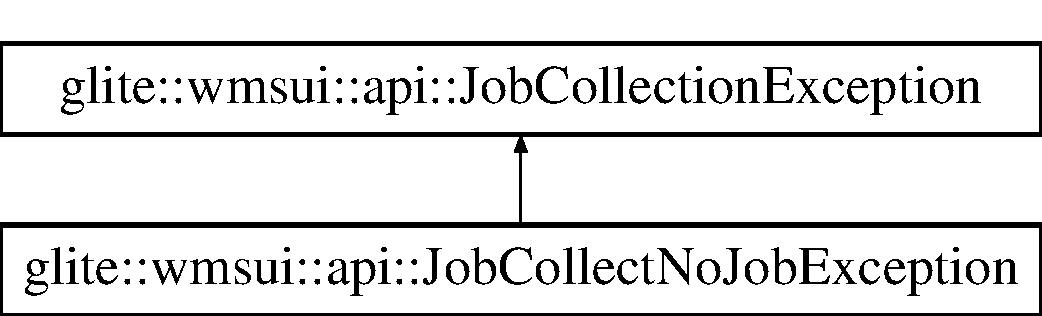
\includegraphics[height=2cm]{classglite_1_1wmsui_1_1api_1_1JobCollectionException}
\end{center}
\end{figure}
\subsection*{Public Member Functions}
\begin{CompactItemize}
\item 
\hyperlink{classglite_1_1wmsui_1_1api_1_1JobCollectionException_a0}{Job\-Collection\-Exception} (const std::string \&file, int line, const std::string \&method, int code, const std::string \&exception\_\-name)
\end{CompactItemize}


\subsection{Detailed Description}
\hyperlink{classglite_1_1wmsui_1_1api_1_1JobCollectionException}{Job\-Collection\-Exception} \begin{Desc}
\item[Version:]0.1 \end{Desc}
\begin{Desc}
\item[Date:]15 April 2002 \end{Desc}
\begin{Desc}
\item[Author:]Alessandro Maraschini $<$\href{mailto:alessandro.maraschini@datamat.it}{\tt alessandro.maraschini@datamat.it}$>$ \end{Desc}




\subsection{Constructor \& Destructor Documentation}
\hypertarget{classglite_1_1wmsui_1_1api_1_1JobCollectionException_a0}{
\index{glite::wmsui::api::JobCollectionException@{glite::wmsui::api::Job\-Collection\-Exception}!JobCollectionException@{JobCollectionException}}
\index{JobCollectionException@{JobCollectionException}!glite::wmsui::api::JobCollectionException@{glite::wmsui::api::Job\-Collection\-Exception}}
\subsubsection[JobCollectionException]{\setlength{\rightskip}{0pt plus 5cm}glite::wmsui::api::Job\-Collection\-Exception::Job\-Collection\-Exception (const std::string \& {\em file}, int {\em line}, const std::string \& {\em method}, int {\em code}, const std::string \& {\em exception\_\-name})}}
\label{classglite_1_1wmsui_1_1api_1_1JobCollectionException_a0}


Update all mandatory Exception Information 

The documentation for this class was generated from the following file:\begin{CompactItemize}
\item 
\hyperlink{JobExceptions_8h}{Job\-Exceptions.h}\end{CompactItemize}

\hypertarget{classglite_1_1wmsui_1_1api_1_1JobCollectNoJobException}{
\section{glite::wmsui::api::Job\-Collect\-No\-Job\-Exception Class Reference}
\label{classglite_1_1wmsui_1_1api_1_1JobCollectNoJobException}\index{glite::wmsui::api::JobCollectNoJobException@{glite::wmsui::api::JobCollectNoJobException}}
}
{\tt \#include $<$Job\-Exceptions.h$>$}

Inheritance diagram for glite::wmsui::api::Job\-Collect\-No\-Job\-Exception::\begin{figure}[H]
\begin{center}
\leavevmode
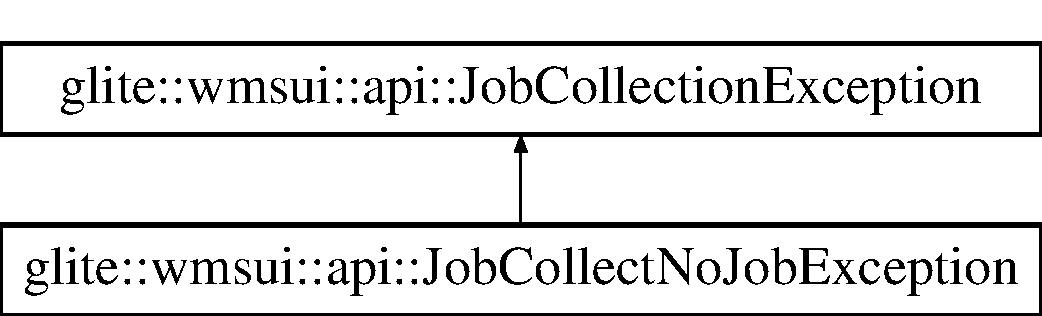
\includegraphics[height=2cm]{classglite_1_1wmsui_1_1api_1_1JobCollectNoJobException}
\end{center}
\end{figure}
\subsection*{Public Member Functions}
\begin{CompactItemize}
\item 
\hyperlink{classglite_1_1wmsui_1_1api_1_1JobCollectNoJobException_a0}{Job\-Collect\-No\-Job\-Exception} (const std::string \&file, int line, const std::string \&method, int code, const std::string \&job=\char`\"{}\char`\"{})
\end{CompactItemize}


\subsection{Detailed Description}
Thrown when an error is found while inserting/deleting jobs 



\subsection{Constructor \& Destructor Documentation}
\hypertarget{classglite_1_1wmsui_1_1api_1_1JobCollectNoJobException_a0}{
\index{glite::wmsui::api::JobCollectNoJobException@{glite::wmsui::api::Job\-Collect\-No\-Job\-Exception}!JobCollectNoJobException@{JobCollectNoJobException}}
\index{JobCollectNoJobException@{JobCollectNoJobException}!glite::wmsui::api::JobCollectNoJobException@{glite::wmsui::api::Job\-Collect\-No\-Job\-Exception}}
\subsubsection[JobCollectNoJobException]{\setlength{\rightskip}{0pt plus 5cm}glite::wmsui::api::Job\-Collect\-No\-Job\-Exception::Job\-Collect\-No\-Job\-Exception (const std::string \& {\em file}, int {\em line}, const std::string \& {\em method}, int {\em code}, const std::string \& {\em job} = \char`\"{}\char`\"{})}}
\label{classglite_1_1wmsui_1_1api_1_1JobCollectNoJobException_a0}


Update all mandatory Exception Information 

The documentation for this class was generated from the following file:\begin{CompactItemize}
\item 
\hyperlink{JobExceptions_8h}{Job\-Exceptions.h}\end{CompactItemize}

\hypertarget{classglite_1_1wmsui_1_1api_1_1JobException}{
\section{glite::wmsui::api::Job\-Exception Class Reference}
\label{classglite_1_1wmsui_1_1api_1_1JobException}\index{glite::wmsui::api::JobException@{glite::wmsui::api::JobException}}
}
{\tt \#include $<$Job\-Exceptions.h$>$}

Inheritance diagram for glite::wmsui::api::Job\-Exception::\begin{figure}[H]
\begin{center}
\leavevmode
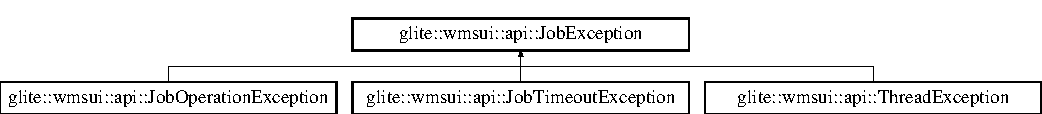
\includegraphics[height=1.53005cm]{classglite_1_1wmsui_1_1api_1_1JobException}
\end{center}
\end{figure}
\subsection*{Protected Member Functions}
\begin{CompactItemize}
\item 
\hyperlink{classglite_1_1wmsui_1_1api_1_1JobException_b0}{Job\-Exception} (const std::string \&file, int line, const std::string \&method, int code, const std::string \&exception\_\-name)
\end{CompactItemize}


\subsection{Detailed Description}
\hyperlink{classglite_1_1wmsui_1_1api_1_1Job}{Job} Exception could be raised from Broker Error \hyperlink{classglite_1_1wmsui_1_1api_1_1Logging}{Logging} Error 



\subsection{Constructor \& Destructor Documentation}
\hypertarget{classglite_1_1wmsui_1_1api_1_1JobException_b0}{
\index{glite::wmsui::api::JobException@{glite::wmsui::api::Job\-Exception}!JobException@{JobException}}
\index{JobException@{JobException}!glite::wmsui::api::JobException@{glite::wmsui::api::Job\-Exception}}
\subsubsection[JobException]{\setlength{\rightskip}{0pt plus 5cm}glite::wmsui::api::Job\-Exception::Job\-Exception (const std::string \& {\em file}, int {\em line}, const std::string \& {\em method}, int {\em code}, const std::string \& {\em exception\_\-name})\hspace{0.3cm}{\tt  \mbox{[}protected\mbox{]}}}}
\label{classglite_1_1wmsui_1_1api_1_1JobException_b0}


Update all mandatory Exception Information 

The documentation for this class was generated from the following file:\begin{CompactItemize}
\item 
\hyperlink{JobExceptions_8h}{Job\-Exceptions.h}\end{CompactItemize}

\hypertarget{classglite_1_1wmsui_1_1api_1_1JobOperationException}{
\section{glite::wmsui::api::Job\-Operation\-Exception Class Reference}
\label{classglite_1_1wmsui_1_1api_1_1JobOperationException}\index{glite::wmsui::api::JobOperationException@{glite::wmsui::api::JobOperationException}}
}
{\tt \#include $<$Job\-Exceptions.h$>$}

Inheritance diagram for glite::wmsui::api::Job\-Operation\-Exception::\begin{figure}[H]
\begin{center}
\leavevmode
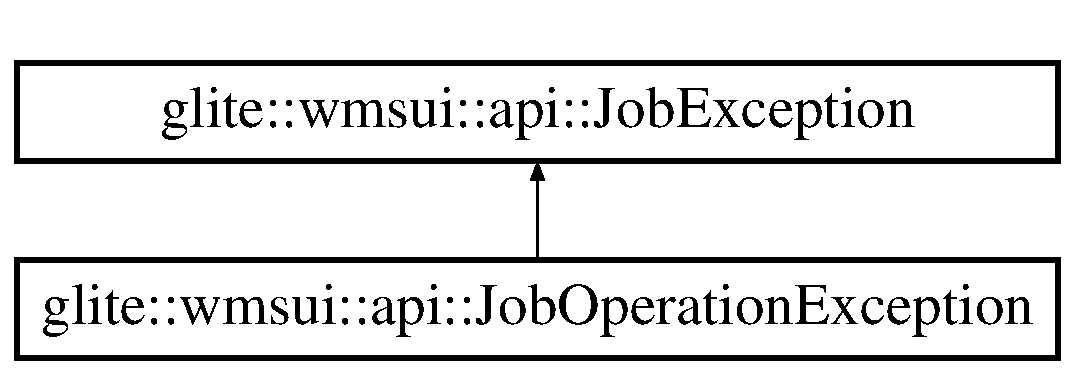
\includegraphics[height=2cm]{classglite_1_1wmsui_1_1api_1_1JobOperationException}
\end{center}
\end{figure}
\subsection*{Public Member Functions}
\begin{CompactItemize}
\item 
\hyperlink{classglite_1_1wmsui_1_1api_1_1JobOperationException_a0}{Job\-Operation\-Exception} (const std::string \&file, int line, const std::string \&method, int code, const std::string \&reason)
\end{CompactItemize}


\subsection{Detailed Description}
Operation not admitted 



\subsection{Constructor \& Destructor Documentation}
\hypertarget{classglite_1_1wmsui_1_1api_1_1JobOperationException_a0}{
\index{glite::wmsui::api::JobOperationException@{glite::wmsui::api::Job\-Operation\-Exception}!JobOperationException@{JobOperationException}}
\index{JobOperationException@{JobOperationException}!glite::wmsui::api::JobOperationException@{glite::wmsui::api::Job\-Operation\-Exception}}
\subsubsection[JobOperationException]{\setlength{\rightskip}{0pt plus 5cm}glite::wmsui::api::Job\-Operation\-Exception::Job\-Operation\-Exception (const std::string \& {\em file}, int {\em line}, const std::string \& {\em method}, int {\em code}, const std::string \& {\em reason})}}
\label{classglite_1_1wmsui_1_1api_1_1JobOperationException_a0}


Update all mandatory Exception Information 

The documentation for this class was generated from the following file:\begin{CompactItemize}
\item 
\hyperlink{JobExceptions_8h}{Job\-Exceptions.h}\end{CompactItemize}

\hypertarget{classglite_1_1wmsui_1_1api_1_1JobTimeoutException}{
\section{glite::wmsui::api::Job\-Timeout\-Exception Class Reference}
\label{classglite_1_1wmsui_1_1api_1_1JobTimeoutException}\index{glite::wmsui::api::JobTimeoutException@{glite::wmsui::api::JobTimeoutException}}
}
{\tt \#include $<$Job\-Exceptions.h$>$}

Inheritance diagram for glite::wmsui::api::Job\-Timeout\-Exception::\begin{figure}[H]
\begin{center}
\leavevmode
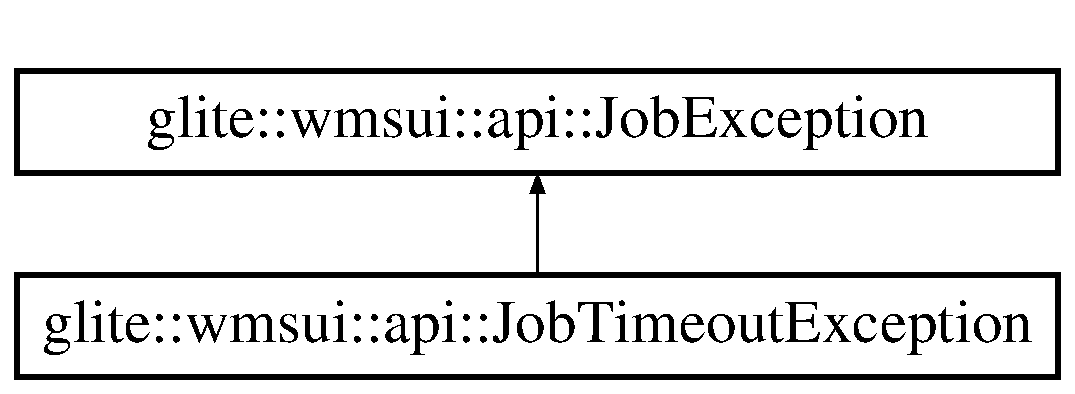
\includegraphics[height=2cm]{classglite_1_1wmsui_1_1api_1_1JobTimeoutException}
\end{center}
\end{figure}
\subsection*{Public Member Functions}
\begin{CompactItemize}
\item 
\hyperlink{classglite_1_1wmsui_1_1api_1_1JobTimeoutException_a0}{Job\-Timeout\-Exception} (const std::string \&file, int line, const std::string \&method, int code)
\end{CompactItemize}


\subsection{Detailed Description}
Operation timeout raised 



\subsection{Constructor \& Destructor Documentation}
\hypertarget{classglite_1_1wmsui_1_1api_1_1JobTimeoutException_a0}{
\index{glite::wmsui::api::JobTimeoutException@{glite::wmsui::api::Job\-Timeout\-Exception}!JobTimeoutException@{JobTimeoutException}}
\index{JobTimeoutException@{JobTimeoutException}!glite::wmsui::api::JobTimeoutException@{glite::wmsui::api::Job\-Timeout\-Exception}}
\subsubsection[JobTimeoutException]{\setlength{\rightskip}{0pt plus 5cm}glite::wmsui::api::Job\-Timeout\-Exception::Job\-Timeout\-Exception (const std::string \& {\em file}, int {\em line}, const std::string \& {\em method}, int {\em code})}}
\label{classglite_1_1wmsui_1_1api_1_1JobTimeoutException_a0}


Update all mandatory Exception Information 

The documentation for this class was generated from the following file:\begin{CompactItemize}
\item 
\hyperlink{JobExceptions_8h}{Job\-Exceptions.h}\end{CompactItemize}

\hypertarget{classglite_1_1wmsui_1_1api_1_1Listener}{
\section{glite::wmsui::api::Listener Class Reference}
\label{classglite_1_1wmsui_1_1api_1_1Listener}\index{glite::wmsui::api::Listener@{glite::wmsui::api::Listener}}
}
{\tt \#include $<$Listener.h$>$}

\subsection*{Public Member Functions}
\begin{CompactItemize}
\item 
virtual void \hyperlink{classglite_1_1wmsui_1_1api_1_1Listener_a0}{run} (\hyperlink{classglite_1_1wmsui_1_1api_1_1Shadow}{Shadow} $\ast$shadow) const=0
\end{CompactItemize}


\subsection{Detailed Description}
The listener interface is used in order to manage the interaction of interactive jobs. 

Depending on how it is implemented, the task of the implemented class should be: \begin{itemize}
\item Reading the output of the job inside the output named pipe \item Prompt the output message to the user (by using a swing window or simply to the std output) \item Catch the standard input from the user and write it to the input name pipe \end{itemize}




\subsection{Member Function Documentation}
\hypertarget{classglite_1_1wmsui_1_1api_1_1Listener_a0}{
\index{glite::wmsui::api::Listener@{glite::wmsui::api::Listener}!run@{run}}
\index{run@{run}!glite::wmsui::api::Listener@{glite::wmsui::api::Listener}}
\subsubsection[run]{\setlength{\rightskip}{0pt plus 5cm}virtual void glite::wmsui::api::Listener::run (\hyperlink{classglite_1_1wmsui_1_1api_1_1Shadow}{Shadow} $\ast$ {\em shadow}) const\hspace{0.3cm}{\tt  \mbox{[}pure virtual\mbox{]}}}}
\label{classglite_1_1wmsui_1_1api_1_1Listener_a0}


This Method is called once the shadow has been successfully launched and the \hyperlink{classglite_1_1wmsui_1_1api_1_1Job}{Job} is ready to perform the interactive console \begin{Desc}
\item[Parameters:]
\begin{description}
\item[{\em shadow}]the \hyperlink{classglite_1_1wmsui_1_1api_1_1Shadow}{Shadow} pointer that stores all the information needed to perform a console interactivity\end{description}
\end{Desc}


The documentation for this class was generated from the following file:\begin{CompactItemize}
\item 
\hyperlink{Listener_8h}{Listener.h}\end{CompactItemize}

\hypertarget{classglite_1_1wmsui_1_1api_1_1Logging}{
\section{glite::wmsui::api::Logging Class Reference}
\label{classglite_1_1wmsui_1_1api_1_1Logging}\index{glite::wmsui::api::Logging@{glite::wmsui::api::Logging}}
}
{\tt \#include $<$Logging.h$>$}

\subsection*{Public Types}
\begin{CompactItemize}
\item 
enum \hyperlink{classglite_1_1wmsui_1_1api_1_1Logging_w3}{tx\-Type} \{ \hyperlink{classglite_1_1wmsui_1_1api_1_1Logging_w3w0}{START}, 
\hyperlink{classglite_1_1wmsui_1_1api_1_1Logging_w3w1}{OK}, 
\hyperlink{classglite_1_1wmsui_1_1api_1_1Logging_w3w2}{FAIL}
 \}
\end{CompactItemize}
\subsection*{Public Member Functions}
\begin{CompactItemize}
\item 
\hyperlink{classglite_1_1wmsui_1_1api_1_1Logging_a0}{Logging} ()
\item 
virtual \hyperlink{classglite_1_1wmsui_1_1api_1_1Logging_a1}{$\sim$Logging} ()  throw ()
\item 
void \hyperlink{classglite_1_1wmsui_1_1api_1_1Logging_a2}{init} (const std::string \&ns\-Host, int ns\-Port, glite::wmsutils::jobid::Job\-Id $\ast$id)
\item 
glite::wms::jdl::Exp\-Dag\-Ad $\ast$ \hyperlink{classglite_1_1wmsui_1_1api_1_1Logging_a3}{register\-Job} (glite::wms::jdl::Job\-Ad $\ast$ad, int resource)
\item 
void \hyperlink{classglite_1_1wmsui_1_1api_1_1Logging_a4}{register\-Job} (glite::wms::jdl::Job\-Ad $\ast$ad)
\item 
void \hyperlink{classglite_1_1wmsui_1_1api_1_1Logging_a5}{register\-Dag} (glite::wms::jdl::Exp\-Dag\-Ad $\ast$ad)
\item 
void \hyperlink{classglite_1_1wmsui_1_1api_1_1Logging_a6}{transfer} (\hyperlink{classglite_1_1wmsui_1_1api_1_1Logging_w3}{tx\-Type} tx, const std::string \&jdl, const char $\ast$error=\char`\"{}\char`\"{})
\item 
std::string \hyperlink{classglite_1_1wmsui_1_1api_1_1Logging_a7}{get\-Sequence} ()
\item 
void \hyperlink{classglite_1_1wmsui_1_1api_1_1Logging_a8}{log\-User\-Tags} (classad::Class\-Ad $\ast$user\-Tags)
\item 
void \hyperlink{classglite_1_1wmsui_1_1api_1_1Logging_a9}{log\-User\-Tags} (std::vector$<$ std::pair$<$ std::string, classad::Expr\-Tree $\ast$ $>$ $>$ user\-Tags)
\end{CompactItemize}


\subsection{Member Enumeration Documentation}
\hypertarget{classglite_1_1wmsui_1_1api_1_1Logging_w3}{
\index{glite::wmsui::api::Logging@{glite::wmsui::api::Logging}!txType@{txType}}
\index{txType@{txType}!glite::wmsui::api::Logging@{glite::wmsui::api::Logging}}
\subsubsection[txType]{\setlength{\rightskip}{0pt plus 5cm}enum \hyperlink{classglite_1_1wmsui_1_1api_1_1Logging_w3}{glite::wmsui::api::Logging::tx\-Type}}}
\label{classglite_1_1wmsui_1_1api_1_1Logging_w3}


\begin{Desc}
\item[Enumeration values: ]\par
\begin{description}
\index{START@{START}!glite::wmsui::api::Logging@{glite::wmsui::api::Logging}}\index{glite::wmsui::api::Logging@{glite::wmsui::api::Logging}!START@{START}}\item[{\em 
\hypertarget{classglite_1_1wmsui_1_1api_1_1Logging_w3w0}{
START}
\label{classglite_1_1wmsui_1_1api_1_1Logging_w3w0}
}]\index{OK@{OK}!glite::wmsui::api::Logging@{glite::wmsui::api::Logging}}\index{glite::wmsui::api::Logging@{glite::wmsui::api::Logging}!OK@{OK}}\item[{\em 
\hypertarget{classglite_1_1wmsui_1_1api_1_1Logging_w3w1}{
OK}
\label{classglite_1_1wmsui_1_1api_1_1Logging_w3w1}
}]\index{FAIL@{FAIL}!glite::wmsui::api::Logging@{glite::wmsui::api::Logging}}\index{glite::wmsui::api::Logging@{glite::wmsui::api::Logging}!FAIL@{FAIL}}\item[{\em 
\hypertarget{classglite_1_1wmsui_1_1api_1_1Logging_w3w2}{
FAIL}
\label{classglite_1_1wmsui_1_1api_1_1Logging_w3w2}
}]\end{description}
\end{Desc}



\subsection{Constructor \& Destructor Documentation}
\hypertarget{classglite_1_1wmsui_1_1api_1_1Logging_a0}{
\index{glite::wmsui::api::Logging@{glite::wmsui::api::Logging}!Logging@{Logging}}
\index{Logging@{Logging}!glite::wmsui::api::Logging@{glite::wmsui::api::Logging}}
\subsubsection[Logging]{\setlength{\rightskip}{0pt plus 5cm}glite::wmsui::api::Logging::Logging ()}}
\label{classglite_1_1wmsui_1_1api_1_1Logging_a0}


\hypertarget{classglite_1_1wmsui_1_1api_1_1Logging_a1}{
\index{glite::wmsui::api::Logging@{glite::wmsui::api::Logging}!~Logging@{$\sim$Logging}}
\index{~Logging@{$\sim$Logging}!glite::wmsui::api::Logging@{glite::wmsui::api::Logging}}
\subsubsection[$\sim$Logging]{\setlength{\rightskip}{0pt plus 5cm}virtual glite::wmsui::api::Logging::$\sim$\hyperlink{classglite_1_1wmsui_1_1api_1_1Logging}{Logging} ()  throw ()\hspace{0.3cm}{\tt  \mbox{[}inline, virtual\mbox{]}}}}
\label{classglite_1_1wmsui_1_1api_1_1Logging_a1}




\subsection{Member Function Documentation}
\hypertarget{classglite_1_1wmsui_1_1api_1_1Logging_a7}{
\index{glite::wmsui::api::Logging@{glite::wmsui::api::Logging}!getSequence@{getSequence}}
\index{getSequence@{getSequence}!glite::wmsui::api::Logging@{glite::wmsui::api::Logging}}
\subsubsection[getSequence]{\setlength{\rightskip}{0pt plus 5cm}std::string glite::wmsui::api::Logging::get\-Sequence ()\hspace{0.3cm}{\tt  \mbox{[}inline\mbox{]}}}}
\label{classglite_1_1wmsui_1_1api_1_1Logging_a7}


\hypertarget{classglite_1_1wmsui_1_1api_1_1Logging_a2}{
\index{glite::wmsui::api::Logging@{glite::wmsui::api::Logging}!init@{init}}
\index{init@{init}!glite::wmsui::api::Logging@{glite::wmsui::api::Logging}}
\subsubsection[init]{\setlength{\rightskip}{0pt plus 5cm}void glite::wmsui::api::Logging::init (const std::string \& {\em ns\-Host}, int {\em ns\-Port}, glite::wmsutils::jobid::Job\-Id $\ast$ {\em id})}}
\label{classglite_1_1wmsui_1_1api_1_1Logging_a2}


\hypertarget{classglite_1_1wmsui_1_1api_1_1Logging_a9}{
\index{glite::wmsui::api::Logging@{glite::wmsui::api::Logging}!logUserTags@{logUserTags}}
\index{logUserTags@{logUserTags}!glite::wmsui::api::Logging@{glite::wmsui::api::Logging}}
\subsubsection[logUserTags]{\setlength{\rightskip}{0pt plus 5cm}void glite::wmsui::api::Logging::log\-User\-Tags (std::vector$<$ std::pair$<$ std::string, classad::Expr\-Tree $\ast$ $>$ $>$ {\em user\-Tags})}}
\label{classglite_1_1wmsui_1_1api_1_1Logging_a9}


\hypertarget{classglite_1_1wmsui_1_1api_1_1Logging_a8}{
\index{glite::wmsui::api::Logging@{glite::wmsui::api::Logging}!logUserTags@{logUserTags}}
\index{logUserTags@{logUserTags}!glite::wmsui::api::Logging@{glite::wmsui::api::Logging}}
\subsubsection[logUserTags]{\setlength{\rightskip}{0pt plus 5cm}void glite::wmsui::api::Logging::log\-User\-Tags (classad::Class\-Ad $\ast$ {\em user\-Tags})}}
\label{classglite_1_1wmsui_1_1api_1_1Logging_a8}


\hypertarget{classglite_1_1wmsui_1_1api_1_1Logging_a5}{
\index{glite::wmsui::api::Logging@{glite::wmsui::api::Logging}!registerDag@{registerDag}}
\index{registerDag@{registerDag}!glite::wmsui::api::Logging@{glite::wmsui::api::Logging}}
\subsubsection[registerDag]{\setlength{\rightskip}{0pt plus 5cm}void glite::wmsui::api::Logging::register\-Dag (glite::wms::jdl::Exp\-Dag\-Ad $\ast$ {\em ad})}}
\label{classglite_1_1wmsui_1_1api_1_1Logging_a5}


\hypertarget{classglite_1_1wmsui_1_1api_1_1Logging_a4}{
\index{glite::wmsui::api::Logging@{glite::wmsui::api::Logging}!registerJob@{registerJob}}
\index{registerJob@{registerJob}!glite::wmsui::api::Logging@{glite::wmsui::api::Logging}}
\subsubsection[registerJob]{\setlength{\rightskip}{0pt plus 5cm}void glite::wmsui::api::Logging::register\-Job (glite::wms::jdl::Job\-Ad $\ast$ {\em ad})}}
\label{classglite_1_1wmsui_1_1api_1_1Logging_a4}


\hypertarget{classglite_1_1wmsui_1_1api_1_1Logging_a3}{
\index{glite::wmsui::api::Logging@{glite::wmsui::api::Logging}!registerJob@{registerJob}}
\index{registerJob@{registerJob}!glite::wmsui::api::Logging@{glite::wmsui::api::Logging}}
\subsubsection[registerJob]{\setlength{\rightskip}{0pt plus 5cm}glite::wms::jdl::Exp\-Dag\-Ad$\ast$ glite::wmsui::api::Logging::register\-Job (glite::wms::jdl::Job\-Ad $\ast$ {\em ad}, int {\em resource})}}
\label{classglite_1_1wmsui_1_1api_1_1Logging_a3}


\hypertarget{classglite_1_1wmsui_1_1api_1_1Logging_a6}{
\index{glite::wmsui::api::Logging@{glite::wmsui::api::Logging}!transfer@{transfer}}
\index{transfer@{transfer}!glite::wmsui::api::Logging@{glite::wmsui::api::Logging}}
\subsubsection[transfer]{\setlength{\rightskip}{0pt plus 5cm}void glite::wmsui::api::Logging::transfer (\hyperlink{classglite_1_1wmsui_1_1api_1_1Logging_w3}{tx\-Type} {\em tx}, const std::string \& {\em jdl}, const char $\ast$ {\em error} = \char`\"{}\char`\"{})}}
\label{classglite_1_1wmsui_1_1api_1_1Logging_a6}




The documentation for this class was generated from the following file:\begin{CompactItemize}
\item 
\hyperlink{Logging_8h}{Logging.h}\end{CompactItemize}

\hypertarget{classglite_1_1wmsui_1_1api_1_1paramStruct}{
\section{glite::wmsui::api::param\-Struct Class Reference}
\label{classglite_1_1wmsui_1_1api_1_1paramStruct}\index{glite::wmsui::api::paramStruct@{glite::wmsui::api::paramStruct}}
}
{\tt \#include $<$Job\-Collection.h$>$}

\subsection*{Friends}
\begin{CompactItemize}
\item 
class \hyperlink{classglite_1_1wmsui_1_1api_1_1paramStruct_n0}{Job\-Collection}
\end{CompactItemize}


\subsection{Friends And Related Function Documentation}
\hypertarget{classglite_1_1wmsui_1_1api_1_1paramStruct_n0}{
\index{glite::wmsui::api::paramStruct@{glite::wmsui::api::param\-Struct}!JobCollection@{JobCollection}}
\index{JobCollection@{JobCollection}!glite::wmsui::api::paramStruct@{glite::wmsui::api::param\-Struct}}
\subsubsection[JobCollection]{\setlength{\rightskip}{0pt plus 5cm}friend class \hyperlink{classglite_1_1wmsui_1_1api_1_1JobCollection}{Job\-Collection}\hspace{0.3cm}{\tt  \mbox{[}friend\mbox{]}}}}
\label{classglite_1_1wmsui_1_1api_1_1paramStruct_n0}




The documentation for this class was generated from the following file:\begin{CompactItemize}
\item 
\hyperlink{JobCollection_8h}{Job\-Collection.h}\end{CompactItemize}

\hypertarget{classglite_1_1wmsui_1_1api_1_1Request}{
\section{glite::wmsui::api::Request Class Reference}
\label{classglite_1_1wmsui_1_1api_1_1Request}\index{glite::wmsui::api::Request@{glite::wmsui::api::Request}}
}
Allow creating the job and controlling it during its lifetime.  


{\tt \#include $<$Request.h$>$}

\subsection*{Public Member Functions}
\begin{Indent}{\bf Constructors/Destructor}\par
\begin{CompactItemize}
\item 
\hyperlink{classglite_1_1wmsui_1_1api_1_1Request_z9_0}{Request} ()
\item 
\hyperlink{classglite_1_1wmsui_1_1api_1_1Request_z9_1}{Request} (const glite::wmsutils::jobid::Job\-Id \&id)
\item 
\hyperlink{classglite_1_1wmsui_1_1api_1_1Request_z9_2}{Request} (const glite::wms::jdl::Exp\-Dag\-Ad \&ad)
\item 
\hyperlink{classglite_1_1wmsui_1_1api_1_1Request_z9_3}{Request} (const glite::wms::jdl::Job\-Ad \&ad)
\item 
\hyperlink{classglite_1_1wmsui_1_1api_1_1Request_z9_4}{Request} (const \hyperlink{classglite_1_1wmsui_1_1api_1_1Request}{Request} \&\hyperlink{classglite_1_1wmsui_1_1api_1_1Request}{Request})
\item 
virtual \hyperlink{classglite_1_1wmsui_1_1api_1_1Request_z9_5}{$\sim$Request} ()  throw ()
\item 
void \hyperlink{classglite_1_1wmsui_1_1api_1_1Request_z9_6}{operator=} (const \hyperlink{classglite_1_1wmsui_1_1api_1_1Request}{Request} \&dag)
\end{CompactItemize}
\end{Indent}
\begin{Indent}{\bf Get/Set Methods}\par
\begin{CompactItemize}
\item 
void \hyperlink{classglite_1_1wmsui_1_1api_1_1Request_z11_0}{set\-Cred\-Path} (const std::string cp)
\item 
void \hyperlink{classglite_1_1wmsui_1_1api_1_1Request_z11_1}{unset\-Cred\-Path} ()
\item 
void \hyperlink{classglite_1_1wmsui_1_1api_1_1Request_z11_2}{set\-Logger\-Level} (unsigned int level)
\item 
void \hyperlink{classglite_1_1wmsui_1_1api_1_1Request_z11_3}{set\-Job\-Ad} (const glite::wms::jdl::Job\-Ad \&ad)
\item 
void \hyperlink{classglite_1_1wmsui_1_1api_1_1Request_z11_4}{set\-Dag\-Ad} (const glite::wms::jdl::Exp\-Dag\-Ad \&ad)
\item 
void \hyperlink{classglite_1_1wmsui_1_1api_1_1Request_z11_5}{set\-Dag\-Id} (const glite::wmsutils::jobid::Job\-Id \&id)
\end{CompactItemize}
\end{Indent}
\begin{Indent}{\bf Job Action Methods}\par
\begin{CompactItemize}
\item 
glite::lb::Job\-Status \hyperlink{classglite_1_1wmsui_1_1api_1_1Request_z13_0}{get\-Status} (bool ad=true)
\item 
std::vector$<$ glite::lb::Event $>$ \hyperlink{classglite_1_1wmsui_1_1api_1_1Request_z13_1}{get\-Log\-Info} ()
\item 
glite::wmsutils::jobid::Job\-Id \hyperlink{classglite_1_1wmsui_1_1api_1_1Request_z13_2}{submit} (const std::string \&ns\-Host, int ns\-Port, const std::string \&lb\-Host, int lb\-Port, const std::string \&ceid=\char`\"{}\char`\"{})
\item 
std::vector$<$ std::string $>$ \hyperlink{classglite_1_1wmsui_1_1api_1_1Request_z13_3}{list\-Matching\-CE} (const std::string \&ns\-Host, int ns\-Port)
\item 
void \hyperlink{classglite_1_1wmsui_1_1api_1_1Request_z13_4}{cancel} ()
\item 
void \hyperlink{classglite_1_1wmsui_1_1api_1_1Request_z13_5}{get\-Output} (const std::string \&dir\_\-path)
\end{CompactItemize}
\end{Indent}


\subsection{Detailed Description}
Allow creating the job and controlling it during its lifetime. 

Allow controlling the Dag The \hyperlink{classglite_1_1wmsui_1_1api_1_1Job}{Job} class provides methods that allow controlling the job during its lifetime. It currently encompasses routines for cancelling a job and retrieving its output, but if needed it will be extended to provide other features such as job checkpointing, holding, releasing etc.

\begin{Desc}
\item[Version:]0.1 \end{Desc}
\begin{Desc}
\item[Date:]15 April 2002 \end{Desc}
\begin{Desc}
\item[Author:]Alessandro Maraschini $<$\href{mailto:alessandro.maraschini@datamat.it}{\tt alessandro.maraschini@datamat.it}$>$ \end{Desc}




\subsection{Constructor \& Destructor Documentation}
\hypertarget{classglite_1_1wmsui_1_1api_1_1Request_z9_0}{
\index{glite::wmsui::api::Request@{glite::wmsui::api::Request}!Request@{Request}}
\index{Request@{Request}!glite::wmsui::api::Request@{glite::wmsui::api::Request}}
\subsubsection[Request]{\setlength{\rightskip}{0pt plus 5cm}glite::wmsui::api::Request::Request ()}}
\label{classglite_1_1wmsui_1_1api_1_1Request_z9_0}


Instantiates an empty \hyperlink{classglite_1_1wmsui_1_1api_1_1Job}{Job} object \hypertarget{classglite_1_1wmsui_1_1api_1_1Request_z9_1}{
\index{glite::wmsui::api::Request@{glite::wmsui::api::Request}!Request@{Request}}
\index{Request@{Request}!glite::wmsui::api::Request@{glite::wmsui::api::Request}}
\subsubsection[Request]{\setlength{\rightskip}{0pt plus 5cm}glite::wmsui::api::Request::Request (const glite::wmsutils::jobid::Job\-Id \& {\em id})}}
\label{classglite_1_1wmsui_1_1api_1_1Request_z9_1}


Instantiates an \hyperlink{classglite_1_1wmsui_1_1api_1_1Job}{Job} object with a Job\-Id \begin{Desc}
\item[Parameters:]
\begin{description}
\item[{\em id}]the Jobid instance \end{description}
\end{Desc}
\begin{Desc}
\item[Exceptions:]
\begin{description}
\item[{\em Job\-Operation\-Exception}]If the Job\-Id is empty \end{description}
\end{Desc}
\hypertarget{classglite_1_1wmsui_1_1api_1_1Request_z9_2}{
\index{glite::wmsui::api::Request@{glite::wmsui::api::Request}!Request@{Request}}
\index{Request@{Request}!glite::wmsui::api::Request@{glite::wmsui::api::Request}}
\subsubsection[Request]{\setlength{\rightskip}{0pt plus 5cm}glite::wmsui::api::Request::Request (const glite::wms::jdl::Exp\-Dag\-Ad \& {\em ad})}}
\label{classglite_1_1wmsui_1_1api_1_1Request_z9_2}


Instantiates an \hyperlink{classglite_1_1wmsui_1_1api_1_1Job}{Job} object with a Exp\-Dag\-Ad \begin{Desc}
\item[Parameters:]
\begin{description}
\item[{\em ad}]the Expr\-Dag\-Ad instance \end{description}
\end{Desc}
\begin{Desc}
\item[Exceptions:]
\begin{description}
\item[{\em Job\-Operation\-Exception}]If the Dag\-Ad is empty \end{description}
\end{Desc}
\hypertarget{classglite_1_1wmsui_1_1api_1_1Request_z9_3}{
\index{glite::wmsui::api::Request@{glite::wmsui::api::Request}!Request@{Request}}
\index{Request@{Request}!glite::wmsui::api::Request@{glite::wmsui::api::Request}}
\subsubsection[Request]{\setlength{\rightskip}{0pt plus 5cm}glite::wmsui::api::Request::Request (const glite::wms::jdl::Job\-Ad \& {\em ad})}}
\label{classglite_1_1wmsui_1_1api_1_1Request_z9_3}


Instantiates an \hyperlink{classglite_1_1wmsui_1_1api_1_1Job}{Job} object with a Job\-Ad \begin{Desc}
\item[Parameters:]
\begin{description}
\item[{\em ad}]the Job\-Ad instance \end{description}
\end{Desc}
\begin{Desc}
\item[Exceptions:]
\begin{description}
\item[{\em Job\-Operation\-Exception}]If the Job\-Ad is empty \end{description}
\end{Desc}
\hypertarget{classglite_1_1wmsui_1_1api_1_1Request_z9_4}{
\index{glite::wmsui::api::Request@{glite::wmsui::api::Request}!Request@{Request}}
\index{Request@{Request}!glite::wmsui::api::Request@{glite::wmsui::api::Request}}
\subsubsection[Request]{\setlength{\rightskip}{0pt plus 5cm}glite::wmsui::api::Request::Request (const \hyperlink{classglite_1_1wmsui_1_1api_1_1Request}{Request} \& {\em Request})}}
\label{classglite_1_1wmsui_1_1api_1_1Request_z9_4}


Copy constructor \hypertarget{classglite_1_1wmsui_1_1api_1_1Request_z9_5}{
\index{glite::wmsui::api::Request@{glite::wmsui::api::Request}!~Request@{$\sim$Request}}
\index{~Request@{$\sim$Request}!glite::wmsui::api::Request@{glite::wmsui::api::Request}}
\subsubsection[$\sim$Request]{\setlength{\rightskip}{0pt plus 5cm}virtual glite::wmsui::api::Request::$\sim$\hyperlink{classglite_1_1wmsui_1_1api_1_1Request}{Request} ()  throw ()\hspace{0.3cm}{\tt  \mbox{[}virtual\mbox{]}}}}
\label{classglite_1_1wmsui_1_1api_1_1Request_z9_5}


destructor 

\subsection{Member Function Documentation}
\hypertarget{classglite_1_1wmsui_1_1api_1_1Request_z13_4}{
\index{glite::wmsui::api::Request@{glite::wmsui::api::Request}!cancel@{cancel}}
\index{cancel@{cancel}!glite::wmsui::api::Request@{glite::wmsui::api::Request}}
\subsubsection[cancel]{\setlength{\rightskip}{0pt plus 5cm}void glite::wmsui::api::Request::cancel ()}}
\label{classglite_1_1wmsui_1_1api_1_1Request_z13_4}


Cancel the job from the Network Server \begin{Desc}
\item[Returns:]The Result of the operation \end{Desc}
\begin{Desc}
\item[Exceptions:]
\begin{description}
\item[{\em Job\-Operation\-Exception}]The Operation required is not allowed for the \hyperlink{classglite_1_1wmsui_1_1api_1_1Job}{Job} \end{description}
\end{Desc}
\begin{Desc}
\item[See also:]exception returned from NS \end{Desc}
\hypertarget{classglite_1_1wmsui_1_1api_1_1Request_z13_1}{
\index{glite::wmsui::api::Request@{glite::wmsui::api::Request}!getLogInfo@{getLogInfo}}
\index{getLogInfo@{getLogInfo}!glite::wmsui::api::Request@{glite::wmsui::api::Request}}
\subsubsection[getLogInfo]{\setlength{\rightskip}{0pt plus 5cm}std::vector$<$glite::lb::Event$>$ glite::wmsui::api::Request::get\-Log\-Info ()}}
\label{classglite_1_1wmsui_1_1api_1_1Request_z13_1}


Retrieve the bookkeeping information of the job \begin{Desc}
\item[Returns:]all the events logged during the job life \end{Desc}
\begin{Desc}
\item[See also:]glite::lb::Event class documentation \end{Desc}
\hypertarget{classglite_1_1wmsui_1_1api_1_1Request_z13_5}{
\index{glite::wmsui::api::Request@{glite::wmsui::api::Request}!getOutput@{getOutput}}
\index{getOutput@{getOutput}!glite::wmsui::api::Request@{glite::wmsui::api::Request}}
\subsubsection[getOutput]{\setlength{\rightskip}{0pt plus 5cm}void glite::wmsui::api::Request::get\-Output (const std::string \& {\em dir\_\-path})}}
\label{classglite_1_1wmsui_1_1api_1_1Request_z13_5}


Retrieve output files of a submitted job \begin{Desc}
\item[Parameters:]
\begin{description}
\item[{\em dir\_\-path}]the path where to retrieve the Output\-Sandbox files \end{description}
\end{Desc}
\begin{Desc}
\item[Exceptions:]
\begin{description}
\item[{\em Job\-Operation\-Exception}]The Operation required is not allowed for the \hyperlink{classglite_1_1wmsui_1_1api_1_1Job}{Job} \end{description}
\end{Desc}
\begin{Desc}
\item[See also:]exception returned from NS \end{Desc}
\hypertarget{classglite_1_1wmsui_1_1api_1_1Request_z13_0}{
\index{glite::wmsui::api::Request@{glite::wmsui::api::Request}!getStatus@{getStatus}}
\index{getStatus@{getStatus}!glite::wmsui::api::Request@{glite::wmsui::api::Request}}
\subsubsection[getStatus]{\setlength{\rightskip}{0pt plus 5cm}glite::lb::Job\-Status glite::wmsui::api::Request::get\-Status (bool {\em ad} = true)}}
\label{classglite_1_1wmsui_1_1api_1_1Request_z13_0}


Retrieve the status of the job \begin{Desc}
\item[Parameters:]
\begin{description}
\item[{\em ad}]if set to false only basic info are retrieved \end{description}
\end{Desc}
\begin{Desc}
\item[Returns:]the status of the requested component \end{Desc}
\begin{Desc}
\item[See also:]glite::lb::Job\-Status class documentation \end{Desc}
\hypertarget{classglite_1_1wmsui_1_1api_1_1Request_z13_3}{
\index{glite::wmsui::api::Request@{glite::wmsui::api::Request}!listMatchingCE@{listMatchingCE}}
\index{listMatchingCE@{listMatchingCE}!glite::wmsui::api::Request@{glite::wmsui::api::Request}}
\subsubsection[listMatchingCE]{\setlength{\rightskip}{0pt plus 5cm}std::vector$<$std::string$>$ glite::wmsui::api::Request::list\-Matching\-CE (const std::string \& {\em ns\-Host}, int {\em ns\-Port})}}
\label{classglite_1_1wmsui_1_1api_1_1Request_z13_3}


Look for matching resources \begin{Desc}
\item[Parameters:]
\begin{description}
\item[{\em ns\-Host}]The Network Server host address \item[{\em ns\-Port}]The Network Server port \end{description}
\end{Desc}
\begin{Desc}
\item[Returns:]the Computing elements that match with the specified JDL \end{Desc}
\hypertarget{classglite_1_1wmsui_1_1api_1_1Request_z9_6}{
\index{glite::wmsui::api::Request@{glite::wmsui::api::Request}!operator=@{operator=}}
\index{operator=@{operator=}!glite::wmsui::api::Request@{glite::wmsui::api::Request}}
\subsubsection[operator=]{\setlength{\rightskip}{0pt plus 5cm}void glite::wmsui::api::Request::operator= (const \hyperlink{classglite_1_1wmsui_1_1api_1_1Request}{Request} \& {\em dag})}}
\label{classglite_1_1wmsui_1_1api_1_1Request_z9_6}


Assignment operator \hypertarget{classglite_1_1wmsui_1_1api_1_1Request_z11_0}{
\index{glite::wmsui::api::Request@{glite::wmsui::api::Request}!setCredPath@{setCredPath}}
\index{setCredPath@{setCredPath}!glite::wmsui::api::Request@{glite::wmsui::api::Request}}
\subsubsection[setCredPath]{\setlength{\rightskip}{0pt plus 5cm}void glite::wmsui::api::Request::set\-Cred\-Path (const std::string {\em cp})}}
\label{classglite_1_1wmsui_1_1api_1_1Request_z11_0}


Set a different Proxy certificate from the default one \begin{Desc}
\item[Parameters:]
\begin{description}
\item[{\em cp}]The full path of the proxy certificate file to be set \end{description}
\end{Desc}
\hypertarget{classglite_1_1wmsui_1_1api_1_1Request_z11_4}{
\index{glite::wmsui::api::Request@{glite::wmsui::api::Request}!setDagAd@{setDagAd}}
\index{setDagAd@{setDagAd}!glite::wmsui::api::Request@{glite::wmsui::api::Request}}
\subsubsection[setDagAd]{\setlength{\rightskip}{0pt plus 5cm}void glite::wmsui::api::Request::set\-Dag\-Ad (const glite::wms::jdl::Exp\-Dag\-Ad \& {\em ad})}}
\label{classglite_1_1wmsui_1_1api_1_1Request_z11_4}


set the Job\-Ad instance \begin{Desc}
\item[Parameters:]
\begin{description}
\item[{\em ad}]the Job\-Ad Instance to set \end{description}
\end{Desc}
\hypertarget{classglite_1_1wmsui_1_1api_1_1Request_z11_5}{
\index{glite::wmsui::api::Request@{glite::wmsui::api::Request}!setDagId@{setDagId}}
\index{setDagId@{setDagId}!glite::wmsui::api::Request@{glite::wmsui::api::Request}}
\subsubsection[setDagId]{\setlength{\rightskip}{0pt plus 5cm}void glite::wmsui::api::Request::set\-Dag\-Id (const glite::wmsutils::jobid::Job\-Id \& {\em id})}}
\label{classglite_1_1wmsui_1_1api_1_1Request_z11_5}


set the Job\-Id instance \begin{Desc}
\item[Parameters:]
\begin{description}
\item[{\em id}]the Job\-Id Instance to set \end{description}
\end{Desc}
\hypertarget{classglite_1_1wmsui_1_1api_1_1Request_z11_3}{
\index{glite::wmsui::api::Request@{glite::wmsui::api::Request}!setJobAd@{setJobAd}}
\index{setJobAd@{setJobAd}!glite::wmsui::api::Request@{glite::wmsui::api::Request}}
\subsubsection[setJobAd]{\setlength{\rightskip}{0pt plus 5cm}void glite::wmsui::api::Request::set\-Job\-Ad (const glite::wms::jdl::Job\-Ad \& {\em ad})}}
\label{classglite_1_1wmsui_1_1api_1_1Request_z11_3}


set the Job\-Ad instance \begin{Desc}
\item[Parameters:]
\begin{description}
\item[{\em ad}]the Job\-Ad Instance to set \end{description}
\end{Desc}
\hypertarget{classglite_1_1wmsui_1_1api_1_1Request_z11_2}{
\index{glite::wmsui::api::Request@{glite::wmsui::api::Request}!setLoggerLevel@{setLoggerLevel}}
\index{setLoggerLevel@{setLoggerLevel}!glite::wmsui::api::Request@{glite::wmsui::api::Request}}
\subsubsection[setLoggerLevel]{\setlength{\rightskip}{0pt plus 5cm}void glite::wmsui::api::Request::set\-Logger\-Level (unsigned int {\em level})\hspace{0.3cm}{\tt  \mbox{[}inline\mbox{]}}}}
\label{classglite_1_1wmsui_1_1api_1_1Request_z11_2}


Se the verbosity level for NS debug \begin{Desc}
\item[Parameters:]
\begin{description}
\item[{\em level}]default value = 0 (no verbosity), max value = 6 (dreadful verbosity, print screen) \end{description}
\end{Desc}
\hypertarget{classglite_1_1wmsui_1_1api_1_1Request_z13_2}{
\index{glite::wmsui::api::Request@{glite::wmsui::api::Request}!submit@{submit}}
\index{submit@{submit}!glite::wmsui::api::Request@{glite::wmsui::api::Request}}
\subsubsection[submit]{\setlength{\rightskip}{0pt plus 5cm}glite::wmsutils::jobid::Job\-Id glite::wmsui::api::Request::submit (const std::string \& {\em ns\-Host}, int {\em ns\-Port}, const std::string \& {\em lb\-Host}, int {\em lb\-Port}, const std::string \& {\em ceid} = \char`\"{}\char`\"{})}}
\label{classglite_1_1wmsui_1_1api_1_1Request_z13_2}


Submit the job to the Network Server \begin{Desc}
\item[Parameters:]
\begin{description}
\item[{\em ns\-Host}]The Network Server host address \item[{\em ns\-Port}]The Network Server port \item[{\em lb\-Host}]The LB Server host address \item[{\em lb\-Port}]The LB Server port \item[{\em ceid}]the resource id where the job has to be executed \end{description}
\end{Desc}
\begin{Desc}
\item[Returns:]the Job\-Id representing the submitted job\end{Desc}
\hypertarget{classglite_1_1wmsui_1_1api_1_1Request_z11_1}{
\index{glite::wmsui::api::Request@{glite::wmsui::api::Request}!unsetCredPath@{unsetCredPath}}
\index{unsetCredPath@{unsetCredPath}!glite::wmsui::api::Request@{glite::wmsui::api::Request}}
\subsubsection[unsetCredPath]{\setlength{\rightskip}{0pt plus 5cm}void glite::wmsui::api::Request::unset\-Cred\-Path ()}}
\label{classglite_1_1wmsui_1_1api_1_1Request_z11_1}


Set the Proxy certificate as default 

The documentation for this class was generated from the following file:\begin{CompactItemize}
\item 
\hyperlink{Request_8h}{Request.h}\end{CompactItemize}

\hypertarget{classglite_1_1wmsui_1_1api_1_1resultStruct}{
\section{glite::wmsui::api::result\-Struct Class Reference}
\label{classglite_1_1wmsui_1_1api_1_1resultStruct}\index{glite::wmsui::api::resultStruct@{glite::wmsui::api::resultStruct}}
}
{\tt \#include $<$Job\-Collection.h$>$}

\subsection*{Public Member Functions}
\begin{CompactItemize}
\item 
\hyperlink{classglite_1_1wmsui_1_1api_1_1resultStruct_a0}{result\-Struct} ()
\item 
Result\-Code \hyperlink{classglite_1_1wmsui_1_1api_1_1resultStruct_a1}{get} ()
\item 
glite::lb::Job\-Status $\ast$ \hyperlink{classglite_1_1wmsui_1_1api_1_1resultStruct_a2}{get\-Status} ()
\item 
std::string \hyperlink{classglite_1_1wmsui_1_1api_1_1resultStruct_a3}{get\-Error} ()
\item 
std::string \hyperlink{classglite_1_1wmsui_1_1api_1_1resultStruct_a4}{get\-Message} ()
\item 
virtual \hyperlink{classglite_1_1wmsui_1_1api_1_1resultStruct_a5}{$\sim$result\-Struct} ()
\end{CompactItemize}
\subsection*{Friends}
\begin{CompactItemize}
\item 
class \hyperlink{classglite_1_1wmsui_1_1api_1_1resultStruct_n0}{Job\-Collection}
\end{CompactItemize}


\subsection{Detailed Description}
This Class is used to return the Result\-Code back to the main function 



\subsection{Constructor \& Destructor Documentation}
\hypertarget{classglite_1_1wmsui_1_1api_1_1resultStruct_a0}{
\index{glite::wmsui::api::resultStruct@{glite::wmsui::api::result\-Struct}!resultStruct@{resultStruct}}
\index{resultStruct@{resultStruct}!glite::wmsui::api::resultStruct@{glite::wmsui::api::result\-Struct}}
\subsubsection[resultStruct]{\setlength{\rightskip}{0pt plus 5cm}glite::wmsui::api::result\-Struct::result\-Struct ()\hspace{0.3cm}{\tt  \mbox{[}inline\mbox{]}}}}
\label{classglite_1_1wmsui_1_1api_1_1resultStruct_a0}


Default Success Constructor \hypertarget{classglite_1_1wmsui_1_1api_1_1resultStruct_a5}{
\index{glite::wmsui::api::resultStruct@{glite::wmsui::api::result\-Struct}!~resultStruct@{$\sim$resultStruct}}
\index{~resultStruct@{$\sim$resultStruct}!glite::wmsui::api::resultStruct@{glite::wmsui::api::result\-Struct}}
\subsubsection[$\sim$resultStruct]{\setlength{\rightskip}{0pt plus 5cm}virtual glite::wmsui::api::result\-Struct::$\sim$\hyperlink{classglite_1_1wmsui_1_1api_1_1resultStruct}{result\-Struct} ()\hspace{0.3cm}{\tt  \mbox{[}inline, virtual\mbox{]}}}}
\label{classglite_1_1wmsui_1_1api_1_1resultStruct_a5}


Destructor 

\subsection{Member Function Documentation}
\hypertarget{classglite_1_1wmsui_1_1api_1_1resultStruct_a1}{
\index{glite::wmsui::api::resultStruct@{glite::wmsui::api::result\-Struct}!get@{get}}
\index{get@{get}!glite::wmsui::api::resultStruct@{glite::wmsui::api::result\-Struct}}
\subsubsection[get]{\setlength{\rightskip}{0pt plus 5cm}Result\-Code glite::wmsui::api::result\-Struct::get ()\hspace{0.3cm}{\tt  \mbox{[}inline\mbox{]}}}}
\label{classglite_1_1wmsui_1_1api_1_1resultStruct_a1}


Used to check the result of the operation, in case of success it returns SUCCES \begin{Desc}
\item[Returns:]the result code of the operation \end{Desc}
\hypertarget{classglite_1_1wmsui_1_1api_1_1resultStruct_a3}{
\index{glite::wmsui::api::resultStruct@{glite::wmsui::api::result\-Struct}!getError@{getError}}
\index{getError@{getError}!glite::wmsui::api::resultStruct@{glite::wmsui::api::result\-Struct}}
\subsubsection[getError]{\setlength{\rightskip}{0pt plus 5cm}std::string glite::wmsui::api::result\-Struct::get\-Error ()\hspace{0.3cm}{\tt  \mbox{[}inline\mbox{]}}}}
\label{classglite_1_1wmsui_1_1api_1_1resultStruct_a3}


If some error occurred (FAILURE result code) retrieve the error message \begin{Desc}
\item[Returns:]A detailed description of the error of the operation \end{Desc}
\hypertarget{classglite_1_1wmsui_1_1api_1_1resultStruct_a4}{
\index{glite::wmsui::api::resultStruct@{glite::wmsui::api::result\-Struct}!getMessage@{getMessage}}
\index{getMessage@{getMessage}!glite::wmsui::api::resultStruct@{glite::wmsui::api::result\-Struct}}
\subsubsection[getMessage]{\setlength{\rightskip}{0pt plus 5cm}std::string glite::wmsui::api::result\-Struct::get\-Message ()\hspace{0.3cm}{\tt  \mbox{[}inline\mbox{]}}}}
\label{classglite_1_1wmsui_1_1api_1_1resultStruct_a4}


Retrieve the message of this result instance \begin{Desc}
\item[Returns:]the string exception (if any) representatio, smpty string otherwise\end{Desc}
\hypertarget{classglite_1_1wmsui_1_1api_1_1resultStruct_a2}{
\index{glite::wmsui::api::resultStruct@{glite::wmsui::api::result\-Struct}!getStatus@{getStatus}}
\index{getStatus@{getStatus}!glite::wmsui::api::resultStruct@{glite::wmsui::api::result\-Struct}}
\subsubsection[getStatus]{\setlength{\rightskip}{0pt plus 5cm}glite::lb::Job\-Status$\ast$ glite::wmsui::api::result\-Struct::get\-Status ()\hspace{0.3cm}{\tt  \mbox{[}inline\mbox{]}}}}
\label{classglite_1_1wmsui_1_1api_1_1resultStruct_a2}


Retrieve the status information from the job If the required operation was a get\-Status then the Job\-Status instance is returned. NULL is returned otherwise. \begin{Desc}
\item[Returns:]the Status attributes information of the job\end{Desc}


\subsection{Friends And Related Function Documentation}
\hypertarget{classglite_1_1wmsui_1_1api_1_1resultStruct_n0}{
\index{glite::wmsui::api::resultStruct@{glite::wmsui::api::result\-Struct}!JobCollection@{JobCollection}}
\index{JobCollection@{JobCollection}!glite::wmsui::api::resultStruct@{glite::wmsui::api::result\-Struct}}
\subsubsection[JobCollection]{\setlength{\rightskip}{0pt plus 5cm}friend class \hyperlink{classglite_1_1wmsui_1_1api_1_1JobCollection}{Job\-Collection}\hspace{0.3cm}{\tt  \mbox{[}friend\mbox{]}}}}
\label{classglite_1_1wmsui_1_1api_1_1resultStruct_n0}




The documentation for this class was generated from the following file:\begin{CompactItemize}
\item 
\hyperlink{JobCollection_8h}{Job\-Collection.h}\end{CompactItemize}

\hypertarget{classglite_1_1wmsui_1_1api_1_1Shadow}{
\section{glite::wmsui::api::Shadow Class Reference}
\label{classglite_1_1wmsui_1_1api_1_1Shadow}\index{glite::wmsui::api::Shadow@{glite::wmsui::api::Shadow}}
}
{\tt \#include $<$Shadow.h$>$}

\subsection*{Public Member Functions}
\begin{CompactItemize}
\item 
void \hyperlink{classglite_1_1wmsui_1_1api_1_1Shadow_a0}{attach} (int port=0)
\item 
std::string \hyperlink{classglite_1_1wmsui_1_1api_1_1Shadow_a1}{empty} (std::string buffer)
\item 
void \hyperlink{classglite_1_1wmsui_1_1api_1_1Shadow_a2}{detach} ()
\item 
void \hyperlink{classglite_1_1wmsui_1_1api_1_1Shadow_a3}{start} ()
\item 
std::string \hyperlink{classglite_1_1wmsui_1_1api_1_1Shadow_a4}{get\-Pipe\-Err} ()
\item 
std::string \hyperlink{classglite_1_1wmsui_1_1api_1_1Shadow_a5}{get\-Pipe\-In} ()
\item 
std::string \hyperlink{classglite_1_1wmsui_1_1api_1_1Shadow_a6}{get\-Pipe\-Out} ()
\item 
int \hyperlink{classglite_1_1wmsui_1_1api_1_1Shadow_a7}{get\-Port} ()
\item 
int \hyperlink{classglite_1_1wmsui_1_1api_1_1Shadow_a8}{get\-Pid} ()
\end{CompactItemize}
\subsection*{Static Public Member Functions}
\begin{CompactItemize}
\item 
std::string \hyperlink{classglite_1_1wmsui_1_1api_1_1Shadow_e0}{get\-Host} ()
\end{CompactItemize}
\subsection*{Friends}
\begin{CompactItemize}
\item 
class \hyperlink{classglite_1_1wmsui_1_1api_1_1Shadow_n0}{Job}
\end{CompactItemize}


\subsection{Detailed Description}
This class provides the core management for interactive jobs. once the glite-grid-console-shadow has started successfully and the job is running the user should interact with the submitted job (or might have attached to a previous job) At the end of the interaction the background bypass process should be killed and the I/O pipes have to be removed. This is done automatically by the 'detach' method. The shadow class must be used togheter with an implementation of the \hyperlink{classglite_1_1wmsui_1_1api_1_1Listener}{Listener} interface, which actually performs the final visual interactivity with the user. \begin{Desc}
\item[See also:]\hyperlink{classglite_1_1wmsui_1_1api_1_1Listener}{Listener} \end{Desc}




\subsection{Member Function Documentation}
\hypertarget{classglite_1_1wmsui_1_1api_1_1Shadow_a0}{
\index{glite::wmsui::api::Shadow@{glite::wmsui::api::Shadow}!attach@{attach}}
\index{attach@{attach}!glite::wmsui::api::Shadow@{glite::wmsui::api::Shadow}}
\subsubsection[attach]{\setlength{\rightskip}{0pt plus 5cm}void glite::wmsui::api::Shadow::attach (int {\em port} = 0)}}
\label{classglite_1_1wmsui_1_1api_1_1Shadow_a0}


Attach a new listener to the \hyperlink{classglite_1_1wmsui_1_1api_1_1Job}{Job} \hypertarget{classglite_1_1wmsui_1_1api_1_1Shadow_a2}{
\index{glite::wmsui::api::Shadow@{glite::wmsui::api::Shadow}!detach@{detach}}
\index{detach@{detach}!glite::wmsui::api::Shadow@{glite::wmsui::api::Shadow}}
\subsubsection[detach]{\setlength{\rightskip}{0pt plus 5cm}void glite::wmsui::api::Shadow::detach ()}}
\label{classglite_1_1wmsui_1_1api_1_1Shadow_a2}


Stop the launched processes and remove the created listener pipes \hypertarget{classglite_1_1wmsui_1_1api_1_1Shadow_a1}{
\index{glite::wmsui::api::Shadow@{glite::wmsui::api::Shadow}!empty@{empty}}
\index{empty@{empty}!glite::wmsui::api::Shadow@{glite::wmsui::api::Shadow}}
\subsubsection[empty]{\setlength{\rightskip}{0pt plus 5cm}std::string glite::wmsui::api::Shadow::empty (std::string {\em buffer})}}
\label{classglite_1_1wmsui_1_1api_1_1Shadow_a1}


Read the specified buffer and return it's content \hypertarget{classglite_1_1wmsui_1_1api_1_1Shadow_e0}{
\index{glite::wmsui::api::Shadow@{glite::wmsui::api::Shadow}!getHost@{getHost}}
\index{getHost@{getHost}!glite::wmsui::api::Shadow@{glite::wmsui::api::Shadow}}
\subsubsection[getHost]{\setlength{\rightskip}{0pt plus 5cm}std::string glite::wmsui::api::Shadow::get\-Host ()\hspace{0.3cm}{\tt  \mbox{[}static\mbox{]}}}}
\label{classglite_1_1wmsui_1_1api_1_1Shadow_e0}


\begin{Desc}
\item[Returns:]the local host name \end{Desc}
\hypertarget{classglite_1_1wmsui_1_1api_1_1Shadow_a8}{
\index{glite::wmsui::api::Shadow@{glite::wmsui::api::Shadow}!getPid@{getPid}}
\index{getPid@{getPid}!glite::wmsui::api::Shadow@{glite::wmsui::api::Shadow}}
\subsubsection[getPid]{\setlength{\rightskip}{0pt plus 5cm}int glite::wmsui::api::Shadow::get\-Pid ()}}
\label{classglite_1_1wmsui_1_1api_1_1Shadow_a8}


Get the process id of the launched listener process \hypertarget{classglite_1_1wmsui_1_1api_1_1Shadow_a4}{
\index{glite::wmsui::api::Shadow@{glite::wmsui::api::Shadow}!getPipeErr@{getPipeErr}}
\index{getPipeErr@{getPipeErr}!glite::wmsui::api::Shadow@{glite::wmsui::api::Shadow}}
\subsubsection[getPipeErr]{\setlength{\rightskip}{0pt plus 5cm}std::string glite::wmsui::api::Shadow::get\-Pipe\-Err ()}}
\label{classglite_1_1wmsui_1_1api_1_1Shadow_a4}


\begin{Desc}
\item[Returns:]the error pipe string representation \end{Desc}
\hypertarget{classglite_1_1wmsui_1_1api_1_1Shadow_a5}{
\index{glite::wmsui::api::Shadow@{glite::wmsui::api::Shadow}!getPipeIn@{getPipeIn}}
\index{getPipeIn@{getPipeIn}!glite::wmsui::api::Shadow@{glite::wmsui::api::Shadow}}
\subsubsection[getPipeIn]{\setlength{\rightskip}{0pt plus 5cm}std::string glite::wmsui::api::Shadow::get\-Pipe\-In ()}}
\label{classglite_1_1wmsui_1_1api_1_1Shadow_a5}


\begin{Desc}
\item[Returns:]the Input pipe string representation \end{Desc}
\hypertarget{classglite_1_1wmsui_1_1api_1_1Shadow_a6}{
\index{glite::wmsui::api::Shadow@{glite::wmsui::api::Shadow}!getPipeOut@{getPipeOut}}
\index{getPipeOut@{getPipeOut}!glite::wmsui::api::Shadow@{glite::wmsui::api::Shadow}}
\subsubsection[getPipeOut]{\setlength{\rightskip}{0pt plus 5cm}std::string glite::wmsui::api::Shadow::get\-Pipe\-Out ()}}
\label{classglite_1_1wmsui_1_1api_1_1Shadow_a6}


\begin{Desc}
\item[Returns:]the Output pipe string representation \end{Desc}
\hypertarget{classglite_1_1wmsui_1_1api_1_1Shadow_a7}{
\index{glite::wmsui::api::Shadow@{glite::wmsui::api::Shadow}!getPort@{getPort}}
\index{getPort@{getPort}!glite::wmsui::api::Shadow@{glite::wmsui::api::Shadow}}
\subsubsection[getPort]{\setlength{\rightskip}{0pt plus 5cm}int glite::wmsui::api::Shadow::get\-Port ()}}
\label{classglite_1_1wmsui_1_1api_1_1Shadow_a7}


Get the port where the shadow is listening to \hypertarget{classglite_1_1wmsui_1_1api_1_1Shadow_a3}{
\index{glite::wmsui::api::Shadow@{glite::wmsui::api::Shadow}!start@{start}}
\index{start@{start}!glite::wmsui::api::Shadow@{glite::wmsui::api::Shadow}}
\subsubsection[start]{\setlength{\rightskip}{0pt plus 5cm}void glite::wmsui::api::Shadow::start ()}}
\label{classglite_1_1wmsui_1_1api_1_1Shadow_a3}


Start the \hyperlink{classglite_1_1wmsui_1_1api_1_1Listener}{Listener} run method \begin{Desc}
\item[See also:]\hyperlink{classglite_1_1wmsui_1_1api_1_1Listener}{Listener}\end{Desc}


\subsection{Friends And Related Function Documentation}
\hypertarget{classglite_1_1wmsui_1_1api_1_1Shadow_n0}{
\index{glite::wmsui::api::Shadow@{glite::wmsui::api::Shadow}!Job@{Job}}
\index{Job@{Job}!glite::wmsui::api::Shadow@{glite::wmsui::api::Shadow}}
\subsubsection[Job]{\setlength{\rightskip}{0pt plus 5cm}friend class \hyperlink{classglite_1_1wmsui_1_1api_1_1Job}{Job}\hspace{0.3cm}{\tt  \mbox{[}friend\mbox{]}}}}
\label{classglite_1_1wmsui_1_1api_1_1Shadow_n0}




The documentation for this class was generated from the following file:\begin{CompactItemize}
\item 
\hyperlink{Shadow_8h}{Shadow.h}\end{CompactItemize}

\hypertarget{classglite_1_1wmsui_1_1api_1_1ThreadException}{
\section{glite::wmsui::api::Thread\-Exception Class Reference}
\label{classglite_1_1wmsui_1_1api_1_1ThreadException}\index{glite::wmsui::api::ThreadException@{glite::wmsui::api::ThreadException}}
}
{\tt \#include $<$Job\-Exceptions.h$>$}

Inheritance diagram for glite::wmsui::api::Thread\-Exception::\begin{figure}[H]
\begin{center}
\leavevmode
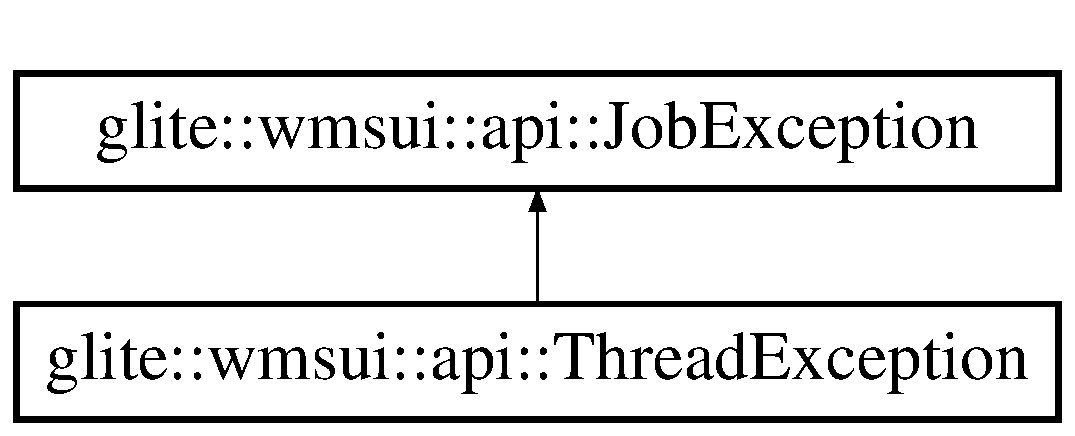
\includegraphics[height=2cm]{classglite_1_1wmsui_1_1api_1_1ThreadException}
\end{center}
\end{figure}
\subsection*{Public Member Functions}
\begin{CompactItemize}
\item 
\hyperlink{classglite_1_1wmsui_1_1api_1_1ThreadException_a0}{Thread\-Exception} (const std::string \&file, int line, const std::string \&method, int code, int job\-Number)
\end{CompactItemize}


\subsection{Detailed Description}
Thrown when a thread is unable to be launched or to run 



\subsection{Constructor \& Destructor Documentation}
\hypertarget{classglite_1_1wmsui_1_1api_1_1ThreadException_a0}{
\index{glite::wmsui::api::ThreadException@{glite::wmsui::api::Thread\-Exception}!ThreadException@{ThreadException}}
\index{ThreadException@{ThreadException}!glite::wmsui::api::ThreadException@{glite::wmsui::api::Thread\-Exception}}
\subsubsection[ThreadException]{\setlength{\rightskip}{0pt plus 5cm}glite::wmsui::api::Thread\-Exception::Thread\-Exception (const std::string \& {\em file}, int {\em line}, const std::string \& {\em method}, int {\em code}, int {\em job\-Number})}}
\label{classglite_1_1wmsui_1_1api_1_1ThreadException_a0}




The documentation for this class was generated from the following file:\begin{CompactItemize}
\item 
\hyperlink{JobExceptions_8h}{Job\-Exceptions.h}\end{CompactItemize}

\hypertarget{classglite_1_1wmsui_1_1api_1_1UserCredential}{
\section{glite::wmsui::api::User\-Credential Class Reference}
\label{classglite_1_1wmsui_1_1api_1_1UserCredential}\index{glite::wmsui::api::UserCredential@{glite::wmsui::api::UserCredential}}
}
Allow getting information about the user credentials.  


{\tt \#include $<$User\-Credential.h$>$}

\subsection*{Public Member Functions}
\begin{CompactItemize}
\item 
\hyperlink{classglite_1_1wmsui_1_1api_1_1UserCredential_a0}{User\-Credential} ()
\item 
int \hyperlink{classglite_1_1wmsui_1_1api_1_1UserCredential_a1}{check\-Proxy} (const std::string \&cred\_\-path=\char`\"{}\char`\"{})
\item 
std::string \hyperlink{classglite_1_1wmsui_1_1api_1_1UserCredential_a2}{get\-Issuer} (const std::string \&cred\_\-path=\char`\"{}\char`\"{})
\item 
std::string \hyperlink{classglite_1_1wmsui_1_1api_1_1UserCredential_a3}{get\-Subject} (const std::string \&cred\_\-path=\char`\"{}\char`\"{})
\item 
int \hyperlink{classglite_1_1wmsui_1_1api_1_1UserCredential_a4}{get\-Cred\-Type} (const std::string \&cred\_\-path=\char`\"{}\char`\"{})
\item 
int \hyperlink{classglite_1_1wmsui_1_1api_1_1UserCredential_a5}{get\-Strenght} (const std::string \&cred\_\-path=\char`\"{}\char`\"{})
\item 
int \hyperlink{classglite_1_1wmsui_1_1api_1_1UserCredential_a6}{get\-Time\-Left} (const std::string \&cred\_\-path=\char`\"{}\char`\"{})
\item 
void \hyperlink{classglite_1_1wmsui_1_1api_1_1UserCredential_a7}{get\-Info} (std::string \&subj, std::string \&issuer, int \&cred\_\-type, int \&strength, int \&time\_\-left, const std::string \&cred\_\-path=\char`\"{}\char`\"{})
\item 
void \hyperlink{classglite_1_1wmsui_1_1api_1_1UserCredential_a8}{destroy} (const std::string \&cred\_\-path=\char`\"{}\char`\"{})
\item 
std::string \hyperlink{classglite_1_1wmsui_1_1api_1_1UserCredential_a9}{get\-Default\-Vo\-Name} ()
\item 
std::vector$<$ std::string $>$ \hyperlink{classglite_1_1wmsui_1_1api_1_1UserCredential_a10}{get\-Vo\-Names} ()
\item 
std::vector$<$ std::string $>$ \hyperlink{classglite_1_1wmsui_1_1api_1_1UserCredential_a11}{get\-Groups} (const std::string \&vo\-Name)
\item 
std::vector$<$ std::string $>$ \hyperlink{classglite_1_1wmsui_1_1api_1_1UserCredential_a12}{get\-Default\-Groups} ()
\item 
bool \hyperlink{classglite_1_1wmsui_1_1api_1_1UserCredential_a13}{contains\-Vo} (const std::string \&vo\-Name)
\end{CompactItemize}


\subsection{Detailed Description}
Allow getting information about the user credentials. 

The \hyperlink{classglite_1_1wmsui_1_1api_1_1UserCredential}{User\-Credential} class provides methods that allow getting information about the user credentials. It does not allow the creation of proxy certificates that have to be generated by using the grid-proxy-init Globus command (the only way of handling credentials that is considered really safe). Namely this is needed since the pass-phrase (very sensitive information) should not be passed through any complex (hence likely to be insecure) software components like GUI. It is recalled that proxy existence and correct setting of the X509$\ast$ variables is required by all job monitoring and control methods. 

This class can manipulate standard proxies as well as VOMS certificates, in order to extract the extension information The main operation are: \begin{itemize}
\item Read a proxy certificate and retrieve any possible information ( time left, subject, strengthetc...) \item Extract and check extensions such as VO name and VO groups from a VOMS certificate \end{itemize}


\begin{Desc}
\item[Version:]0.1 \end{Desc}
\begin{Desc}
\item[Date:]15 April 2002 \end{Desc}
\begin{Desc}
\item[Author:]Alessandro Maraschini $<$\href{mailto:alessandro.maraschini@datamat.it}{\tt alessandro.maraschini@datamat.it}$>$ \end{Desc}




\subsection{Constructor \& Destructor Documentation}
\hypertarget{classglite_1_1wmsui_1_1api_1_1UserCredential_a0}{
\index{glite::wmsui::api::UserCredential@{glite::wmsui::api::User\-Credential}!UserCredential@{UserCredential}}
\index{UserCredential@{UserCredential}!glite::wmsui::api::UserCredential@{glite::wmsui::api::User\-Credential}}
\subsubsection[UserCredential]{\setlength{\rightskip}{0pt plus 5cm}glite::wmsui::api::User\-Credential::User\-Credential ()\hspace{0.3cm}{\tt  \mbox{[}inline\mbox{]}}}}
\label{classglite_1_1wmsui_1_1api_1_1UserCredential_a0}


Empty Constructor 

\subsection{Member Function Documentation}
\hypertarget{classglite_1_1wmsui_1_1api_1_1UserCredential_a1}{
\index{glite::wmsui::api::UserCredential@{glite::wmsui::api::User\-Credential}!checkProxy@{checkProxy}}
\index{checkProxy@{checkProxy}!glite::wmsui::api::UserCredential@{glite::wmsui::api::User\-Credential}}
\subsubsection[checkProxy]{\setlength{\rightskip}{0pt plus 5cm}int glite::wmsui::api::User\-Credential::check\-Proxy (const std::string \& {\em cred\_\-path} = \char`\"{}\char`\"{})}}
\label{classglite_1_1wmsui_1_1api_1_1UserCredential_a1}


Check if the Proxy Certificate is valid \begin{Desc}
\item[Parameters:]
\begin{description}
\item[{\em cred\_\-path}]the whole path of the proxy Certificate (if different from the default one) \end{description}
\end{Desc}
\begin{Desc}
\item[Exceptions:]
\begin{description}
\item[{\em Proxy\-Exception}]The proxy certificate is not valid \item[{\em Cred\-Proxy\-Exception}]Unable to get the proxy certificate\end{description}
\end{Desc}
\hypertarget{classglite_1_1wmsui_1_1api_1_1UserCredential_a13}{
\index{glite::wmsui::api::UserCredential@{glite::wmsui::api::User\-Credential}!containsVo@{containsVo}}
\index{containsVo@{containsVo}!glite::wmsui::api::UserCredential@{glite::wmsui::api::User\-Credential}}
\subsubsection[containsVo]{\setlength{\rightskip}{0pt plus 5cm}bool glite::wmsui::api::User\-Credential::contains\-Vo (const std::string \& {\em vo\-Name})}}
\label{classglite_1_1wmsui_1_1api_1_1UserCredential_a13}


Check wheater the specifie Virtual Organisation is contained in the Vo certificate extension \begin{Desc}
\item[Returns:]true if the Vo\-Name is present, false otherwise\end{Desc}
\hypertarget{classglite_1_1wmsui_1_1api_1_1UserCredential_a8}{
\index{glite::wmsui::api::UserCredential@{glite::wmsui::api::User\-Credential}!destroy@{destroy}}
\index{destroy@{destroy}!glite::wmsui::api::UserCredential@{glite::wmsui::api::User\-Credential}}
\subsubsection[destroy]{\setlength{\rightskip}{0pt plus 5cm}void glite::wmsui::api::User\-Credential::destroy (const std::string \& {\em cred\_\-path} = \char`\"{}\char`\"{})}}
\label{classglite_1_1wmsui_1_1api_1_1UserCredential_a8}


Destroy the proxy file (if present) \begin{Desc}
\item[Parameters:]
\begin{description}
\item[{\em cred\_\-path}]the whole path of the proxy Certificate (if different from the default one)\end{description}
\end{Desc}
\hypertarget{classglite_1_1wmsui_1_1api_1_1UserCredential_a4}{
\index{glite::wmsui::api::UserCredential@{glite::wmsui::api::User\-Credential}!getCredType@{getCredType}}
\index{getCredType@{getCredType}!glite::wmsui::api::UserCredential@{glite::wmsui::api::User\-Credential}}
\subsubsection[getCredType]{\setlength{\rightskip}{0pt plus 5cm}int glite::wmsui::api::User\-Credential::get\-Cred\-Type (const std::string \& {\em cred\_\-path} = \char`\"{}\char`\"{})}}
\label{classglite_1_1wmsui_1_1api_1_1UserCredential_a4}


Return the Subject of the Proxy Certificate \begin{Desc}
\item[Parameters:]
\begin{description}
\item[{\em cred\_\-path}]the whole path of the proxy Certificate (if different from the default one) \end{description}
\end{Desc}
\begin{Desc}
\item[Exceptions:]
\begin{description}
\item[{\em Cred\-Proxy\-Exception}]Unable to get the proxy certificate\end{description}
\end{Desc}
\hypertarget{classglite_1_1wmsui_1_1api_1_1UserCredential_a12}{
\index{glite::wmsui::api::UserCredential@{glite::wmsui::api::User\-Credential}!getDefaultGroups@{getDefaultGroups}}
\index{getDefaultGroups@{getDefaultGroups}!glite::wmsui::api::UserCredential@{glite::wmsui::api::User\-Credential}}
\subsubsection[getDefaultGroups]{\setlength{\rightskip}{0pt plus 5cm}std::vector$<$std::string $>$ glite::wmsui::api::User\-Credential::get\-Default\-Groups ()}}
\label{classglite_1_1wmsui_1_1api_1_1UserCredential_a12}


Returns the groups belonging to the default Virtual\-Organisation \hypertarget{classglite_1_1wmsui_1_1api_1_1UserCredential_a9}{
\index{glite::wmsui::api::UserCredential@{glite::wmsui::api::User\-Credential}!getDefaultVoName@{getDefaultVoName}}
\index{getDefaultVoName@{getDefaultVoName}!glite::wmsui::api::UserCredential@{glite::wmsui::api::User\-Credential}}
\subsubsection[getDefaultVoName]{\setlength{\rightskip}{0pt plus 5cm}std::string glite::wmsui::api::User\-Credential::get\-Default\-Vo\-Name ()}}
\label{classglite_1_1wmsui_1_1api_1_1UserCredential_a9}


Retrieve the default Virtual Organisation name \hypertarget{classglite_1_1wmsui_1_1api_1_1UserCredential_a11}{
\index{glite::wmsui::api::UserCredential@{glite::wmsui::api::User\-Credential}!getGroups@{getGroups}}
\index{getGroups@{getGroups}!glite::wmsui::api::UserCredential@{glite::wmsui::api::User\-Credential}}
\subsubsection[getGroups]{\setlength{\rightskip}{0pt plus 5cm}std::vector$<$std::string$>$ glite::wmsui::api::User\-Credential::get\-Groups (const std::string \& {\em vo\-Name})}}
\label{classglite_1_1wmsui_1_1api_1_1UserCredential_a11}


Retrieve all groups belonging to the specified Virtual\-Organisation \begin{Desc}
\item[Parameters:]
\begin{description}
\item[{\em vo\-Name}]the name of the Virtual Organisation where to retrieve groups \end{description}
\end{Desc}
\hypertarget{classglite_1_1wmsui_1_1api_1_1UserCredential_a7}{
\index{glite::wmsui::api::UserCredential@{glite::wmsui::api::User\-Credential}!getInfo@{getInfo}}
\index{getInfo@{getInfo}!glite::wmsui::api::UserCredential@{glite::wmsui::api::User\-Credential}}
\subsubsection[getInfo]{\setlength{\rightskip}{0pt plus 5cm}void glite::wmsui::api::User\-Credential::get\-Info (std::string \& {\em subj}, std::string \& {\em issuer}, int \& {\em cred\_\-type}, int \& {\em strength}, int \& {\em time\_\-left}, const std::string \& {\em cred\_\-path} = \char`\"{}\char`\"{})}}
\label{classglite_1_1wmsui_1_1api_1_1UserCredential_a7}


Return the lasting time of the Proxy Certificate \begin{Desc}
\item[Parameters:]
\begin{description}
\item[{\em subj}]a std::string variable where the subject will be copied to \item[{\em issuer}]a std::string variable where the issuer will be copied to \item[{\em cred\_\-type}]an int variable where the cred type will be copied to \item[{\em strength}]an int variable where the strength will be copied to \item[{\em time\_\-left}]an int variable where the time left will be copied to \item[{\em cred\_\-path}]the whole path of the proxy Certificate (if different from the default one) \end{description}
\end{Desc}
\begin{Desc}
\item[Exceptions:]
\begin{description}
\item[{\em Cred\-Proxy\-Exception}]Unable to get the proxy certificate\end{description}
\end{Desc}
\hypertarget{classglite_1_1wmsui_1_1api_1_1UserCredential_a2}{
\index{glite::wmsui::api::UserCredential@{glite::wmsui::api::User\-Credential}!getIssuer@{getIssuer}}
\index{getIssuer@{getIssuer}!glite::wmsui::api::UserCredential@{glite::wmsui::api::User\-Credential}}
\subsubsection[getIssuer]{\setlength{\rightskip}{0pt plus 5cm}std::string glite::wmsui::api::User\-Credential::get\-Issuer (const std::string \& {\em cred\_\-path} = \char`\"{}\char`\"{})}}
\label{classglite_1_1wmsui_1_1api_1_1UserCredential_a2}


Return the Issuer of the Proxy Certificate \begin{Desc}
\item[Parameters:]
\begin{description}
\item[{\em cred\_\-path}]the whole path of the proxy Certificate (if different from the default one) \end{description}
\end{Desc}
\begin{Desc}
\item[Exceptions:]
\begin{description}
\item[{\em Cred\-Proxy\-Exception}]Unable to get the proxy certificate\end{description}
\end{Desc}
\hypertarget{classglite_1_1wmsui_1_1api_1_1UserCredential_a5}{
\index{glite::wmsui::api::UserCredential@{glite::wmsui::api::User\-Credential}!getStrenght@{getStrenght}}
\index{getStrenght@{getStrenght}!glite::wmsui::api::UserCredential@{glite::wmsui::api::User\-Credential}}
\subsubsection[getStrenght]{\setlength{\rightskip}{0pt plus 5cm}int glite::wmsui::api::User\-Credential::get\-Strenght (const std::string \& {\em cred\_\-path} = \char`\"{}\char`\"{})}}
\label{classglite_1_1wmsui_1_1api_1_1UserCredential_a5}


Return the Cred type of the Proxy Certificate \begin{Desc}
\item[Parameters:]
\begin{description}
\item[{\em cred\_\-path}]the whole path of the proxy Certificate (if different from the default one) \end{description}
\end{Desc}
\begin{Desc}
\item[Exceptions:]
\begin{description}
\item[{\em Cred\-Proxy\-Exception}]Unable to get the proxy certificate\end{description}
\end{Desc}
\hypertarget{classglite_1_1wmsui_1_1api_1_1UserCredential_a3}{
\index{glite::wmsui::api::UserCredential@{glite::wmsui::api::User\-Credential}!getSubject@{getSubject}}
\index{getSubject@{getSubject}!glite::wmsui::api::UserCredential@{glite::wmsui::api::User\-Credential}}
\subsubsection[getSubject]{\setlength{\rightskip}{0pt plus 5cm}std::string glite::wmsui::api::User\-Credential::get\-Subject (const std::string \& {\em cred\_\-path} = \char`\"{}\char`\"{})}}
\label{classglite_1_1wmsui_1_1api_1_1UserCredential_a3}


Return the Issuer of the Proxy Certificate \begin{Desc}
\item[Parameters:]
\begin{description}
\item[{\em cred\_\-path}]the whole path of the proxy Certificate (if different from the default one) \end{description}
\end{Desc}
\begin{Desc}
\item[Exceptions:]
\begin{description}
\item[{\em Cred\-Proxy\-Exception}]Unable to get the proxy certificate\end{description}
\end{Desc}
\hypertarget{classglite_1_1wmsui_1_1api_1_1UserCredential_a6}{
\index{glite::wmsui::api::UserCredential@{glite::wmsui::api::User\-Credential}!getTimeLeft@{getTimeLeft}}
\index{getTimeLeft@{getTimeLeft}!glite::wmsui::api::UserCredential@{glite::wmsui::api::User\-Credential}}
\subsubsection[getTimeLeft]{\setlength{\rightskip}{0pt plus 5cm}int glite::wmsui::api::User\-Credential::get\-Time\-Left (const std::string \& {\em cred\_\-path} = \char`\"{}\char`\"{})}}
\label{classglite_1_1wmsui_1_1api_1_1UserCredential_a6}


Return the Strenght of the Proxy Certificate \begin{Desc}
\item[Parameters:]
\begin{description}
\item[{\em cred\_\-path}]the whole path of the proxy Certificate (if different from the default one) \end{description}
\end{Desc}
\begin{Desc}
\item[Exceptions:]
\begin{description}
\item[{\em Cred\-Proxy\-Exception}]Unable to get the proxy certificate\end{description}
\end{Desc}
\hypertarget{classglite_1_1wmsui_1_1api_1_1UserCredential_a10}{
\index{glite::wmsui::api::UserCredential@{glite::wmsui::api::User\-Credential}!getVoNames@{getVoNames}}
\index{getVoNames@{getVoNames}!glite::wmsui::api::UserCredential@{glite::wmsui::api::User\-Credential}}
\subsubsection[getVoNames]{\setlength{\rightskip}{0pt plus 5cm}std::vector$<$std::string$>$ glite::wmsui::api::User\-Credential::get\-Vo\-Names ()}}
\label{classglite_1_1wmsui_1_1api_1_1UserCredential_a10}


Retrieve the vector of all the Virtual Organisation names 

The documentation for this class was generated from the following file:\begin{CompactItemize}
\item 
\hyperlink{UserCredential_8h}{User\-Credential.h}\end{CompactItemize}

\hypertarget{classglite_1_1wmsui_1_1api_1_1UserJobs}{
\section{glite::wmsui::api::User\-Jobs Class Reference}
\label{classglite_1_1wmsui_1_1api_1_1UserJobs}\index{glite::wmsui::api::UserJobs@{glite::wmsui::api::UserJobs}}
}
Allow controlling all the jobs owned by the user.  


{\tt \#include $<$User\-Jobs.h$>$}

\subsection*{Public Member Functions}
\begin{Indent}{\bf Constructors/Destructor}\par
\begin{CompactItemize}
\item 
\hyperlink{classglite_1_1wmsui_1_1api_1_1UserJobs_z27_0}{User\-Jobs} ()
\item 
\hyperlink{classglite_1_1wmsui_1_1api_1_1UserJobs_z27_1}{$\sim$User\-Jobs} ()
\item 
\hyperlink{classglite_1_1wmsui_1_1api_1_1UserJobs_z27_2}{User\-Jobs} (const std::string cred\_\-path)
\end{CompactItemize}
\end{Indent}
\begin{Indent}{\bf Action Methods}\par
\begin{CompactItemize}
\item 
void \hyperlink{classglite_1_1wmsui_1_1api_1_1UserJobs_z29_0}{get\-Jobs} (const std::string \&lb\-Host, int lb\-Port, std::vector$<$ glite::wmsutils::jobid::Job\-Id $>$ \&jobs)
\item 
void \hyperlink{classglite_1_1wmsui_1_1api_1_1UserJobs_z29_1}{get\-Status} (const std::string \&lb\-Host, int lb\-Port, std::vector$<$ glite::lb::Job\-Status $>$ \&jobs\-Status)
\end{CompactItemize}
\end{Indent}


\subsection{Detailed Description}
Allow controlling all the jobs owned by the user. 

Allow controlling all the jobs owned by the user The \hyperlink{classglite_1_1wmsui_1_1api_1_1UserJobs}{User\-Jobs} class provides methods that allow controlling all the user's jobs during its lifetime. such as getting their status, or cancelling them

\begin{Desc}
\item[Version:]0.1 \end{Desc}
\begin{Desc}
\item[Date:]15 April 2002 \end{Desc}
\begin{Desc}
\item[Author:]Alessandro Maraschini $<$\href{mailto:alessandro.maraschini@datamat.it}{\tt alessandro.maraschini@datamat.it}$>$ \end{Desc}




\subsection{Constructor \& Destructor Documentation}
\hypertarget{classglite_1_1wmsui_1_1api_1_1UserJobs_z27_0}{
\index{glite::wmsui::api::UserJobs@{glite::wmsui::api::User\-Jobs}!UserJobs@{UserJobs}}
\index{UserJobs@{UserJobs}!glite::wmsui::api::UserJobs@{glite::wmsui::api::User\-Jobs}}
\subsubsection[UserJobs]{\setlength{\rightskip}{0pt plus 5cm}glite::wmsui::api::User\-Jobs::User\-Jobs ()}}
\label{classglite_1_1wmsui_1_1api_1_1UserJobs_z27_0}


Instantiates an \hyperlink{classglite_1_1wmsui_1_1api_1_1UserJobs}{User\-Jobs} object using default user credential \hypertarget{classglite_1_1wmsui_1_1api_1_1UserJobs_z27_1}{
\index{glite::wmsui::api::UserJobs@{glite::wmsui::api::User\-Jobs}!~UserJobs@{$\sim$UserJobs}}
\index{~UserJobs@{$\sim$UserJobs}!glite::wmsui::api::UserJobs@{glite::wmsui::api::User\-Jobs}}
\subsubsection[$\sim$UserJobs]{\setlength{\rightskip}{0pt plus 5cm}glite::wmsui::api::User\-Jobs::$\sim$\hyperlink{classglite_1_1wmsui_1_1api_1_1UserJobs}{User\-Jobs} ()}}
\label{classglite_1_1wmsui_1_1api_1_1UserJobs_z27_1}


Destructor \hypertarget{classglite_1_1wmsui_1_1api_1_1UserJobs_z27_2}{
\index{glite::wmsui::api::UserJobs@{glite::wmsui::api::User\-Jobs}!UserJobs@{UserJobs}}
\index{UserJobs@{UserJobs}!glite::wmsui::api::UserJobs@{glite::wmsui::api::User\-Jobs}}
\subsubsection[UserJobs]{\setlength{\rightskip}{0pt plus 5cm}glite::wmsui::api::User\-Jobs::User\-Jobs (const std::string {\em cred\_\-path})}}
\label{classglite_1_1wmsui_1_1api_1_1UserJobs_z27_2}


Instantiates an \hyperlink{classglite_1_1wmsui_1_1api_1_1UserJobs}{User\-Jobs} object using non-default credential \begin{Desc}
\item[Parameters:]
\begin{description}
\item[{\em cred\_\-path}]The proxy certificate file where to retrive credential from \end{description}
\end{Desc}


\subsection{Member Function Documentation}
\hypertarget{classglite_1_1wmsui_1_1api_1_1UserJobs_z29_0}{
\index{glite::wmsui::api::UserJobs@{glite::wmsui::api::User\-Jobs}!getJobs@{getJobs}}
\index{getJobs@{getJobs}!glite::wmsui::api::UserJobs@{glite::wmsui::api::User\-Jobs}}
\subsubsection[getJobs]{\setlength{\rightskip}{0pt plus 5cm}void glite::wmsui::api::User\-Jobs::get\-Jobs (const std::string \& {\em lb\-Host}, int {\em lb\-Port}, std::vector$<$ glite::wmsutils::jobid::Job\-Id $>$ \& {\em jobs})}}
\label{classglite_1_1wmsui_1_1api_1_1UserJobs_z29_0}


Retreive the jobs owned by the user in a specific LB \begin{Desc}
\item[Parameters:]
\begin{description}
\item[{\em lb\-Host}]the LB server host name \item[{\em lb\-Port}]the LB server port value \item[{\em jobs}]the vector of Job\-Id which will be filled with all the user jobs\end{description}
\end{Desc}
\hypertarget{classglite_1_1wmsui_1_1api_1_1UserJobs_z29_1}{
\index{glite::wmsui::api::UserJobs@{glite::wmsui::api::User\-Jobs}!getStatus@{getStatus}}
\index{getStatus@{getStatus}!glite::wmsui::api::UserJobs@{glite::wmsui::api::User\-Jobs}}
\subsubsection[getStatus]{\setlength{\rightskip}{0pt plus 5cm}void glite::wmsui::api::User\-Jobs::get\-Status (const std::string \& {\em lb\-Host}, int {\em lb\-Port}, std::vector$<$ glite::lb::Job\-Status $>$ \& {\em jobs\-Status})}}
\label{classglite_1_1wmsui_1_1api_1_1UserJobs_z29_1}


Retrieve the status of all the user's jobs \begin{Desc}
\item[Parameters:]
\begin{description}
\item[{\em lb\-Host}]the LB server host name \item[{\em lb\-Port}]the LB server port value \item[{\em jobs\-Status}]the vector to be filled of all the jobs status information \end{description}
\end{Desc}


The documentation for this class was generated from the following file:\begin{CompactItemize}
\item 
\hyperlink{UserJobs_8h}{User\-Jobs.h}\end{CompactItemize}


}



\subsection{Job Description API---C++ binding}
\label{jdlcpp}
{
\renewenvironment{CompactList}{\itemize\itemsep -2pt}{\enditemize}
\def\section#1{}
\renewcommand{\contentsline}[4]{{\bf #2}\leaders\hbox{.}\hfill #3}
The documentation of C$++$ Job Description API (also referred to as JDL API) presented in this section was 
generated automatically from the comments in the API header files by Doxygen.
The packages providing the Job Description API are {\verb!org.glite.wms.jdl!} and {\verb!org.glite.wms.jdlj!}.


The class hierarchy is depicted in the following list.
\section{Glite JDL API: CPP Documentation Class Hierarchy}
This inheritance list is sorted roughly, but not completely, alphabetically:\begin{CompactList}
\item \contentsline{section}{glite::wms::jdl::Ad}{\pageref{classglite_1_1wms_1_1jdl_1_1Ad}}{}
\begin{CompactList}
\item \contentsline{section}{glite::wms::jdl::Job\-Ad}{\pageref{classglite_1_1wms_1_1jdl_1_1JobAd}}{}
\begin{CompactList}
\item \contentsline{section}{glite::wms::jdl::Node\-Ad}{\pageref{classglite_1_1wms_1_1jdl_1_1NodeAd}}{}
\end{CompactList}
\end{CompactList}
\item \contentsline{section}{glite::wms::jdl::Ad\-Converter}{\pageref{classglite_1_1wms_1_1jdl_1_1AdConverter}}{}
\item \contentsline{section}{glite::wms::jdl::DAGAd}{\pageref{classglite_1_1wms_1_1jdl_1_1DAGAd}}{}
\item \contentsline{section}{glite::wms::jdl::DAGAd::Attributes}{\pageref{structglite_1_1wms_1_1jdl_1_1DAGAd_1_1Attributes}}{}
\item \contentsline{section}{glite::wms::jdl::DAGAd\-Dependency\-Iterator}{\pageref{structglite_1_1wms_1_1jdl_1_1DAGAdDependencyIterator}}{}
\item \contentsline{section}{glite::wms::jdl::DAGAd\-Node\-Iterator}{\pageref{classglite_1_1wms_1_1jdl_1_1DAGAdNodeIterator}}{}
\item \contentsline{section}{glite::wms::jdl::DAGNode\-Info}{\pageref{classglite_1_1wms_1_1jdl_1_1DAGNodeInfo}}{}
\item \contentsline{section}{glite::wms::jdl::Exp\-Dag\-Ad}{\pageref{classglite_1_1wms_1_1jdl_1_1ExpDagAd}}{}
\item \contentsline{section}{glite::wms::jdl::Invalid\-DAG}{\pageref{structglite_1_1wms_1_1jdl_1_1InvalidDAG}}{}
\item \contentsline{section}{glite::wms::jdl::Invalid\-Node\-Info}{\pageref{structglite_1_1wms_1_1jdl_1_1InvalidNodeInfo}}{}
\item \contentsline{section}{glite::wms::jdl::Jdl\-Attribute\-List}{\pageref{classglite_1_1wms_1_1jdl_1_1JdlAttributeList}}{}
\item \contentsline{section}{glite::wms::jdl::Job\-Ad\-Schema}{\pageref{classglite_1_1wms_1_1jdl_1_1JobAdSchema}}{}
\item \contentsline{section}{glite::wms::jdl::Job\-Id\-Struct}{\pageref{structglite_1_1wms_1_1jdl_1_1JobIdStruct}}{}
\item \contentsline{section}{glite::wms::jdl::Manipulation\-Exception}{\pageref{classglite_1_1wms_1_1jdl_1_1ManipulationException}}{}
\begin{CompactList}
\item \contentsline{section}{glite::wms::jdl::Cannot\-Get\-Attribute}{\pageref{classglite_1_1wms_1_1jdl_1_1CannotGetAttribute}}{}
\item \contentsline{section}{glite::wms::jdl::Cannot\-Remove\-Attribute}{\pageref{classglite_1_1wms_1_1jdl_1_1CannotRemoveAttribute}}{}
\item \contentsline{section}{glite::wms::jdl::Cannot\-Set\-Attribute}{\pageref{classglite_1_1wms_1_1jdl_1_1CannotSetAttribute}}{}
\end{CompactList}
\item \contentsline{section}{glite::wms::jdl::Node\-Struct}{\pageref{structglite_1_1wms_1_1jdl_1_1NodeStruct}}{}
\item \contentsline{section}{glite::wms::jdl::Request\-Ad\-Exception}{\pageref{classglite_1_1wms_1_1jdl_1_1RequestAdException}}{}
\begin{CompactList}
\item \contentsline{section}{glite::wms::jdl::Ad\-Attribute\-Exception}{\pageref{classglite_1_1wms_1_1jdl_1_1AdAttributeException}}{}
\begin{CompactList}
\item \contentsline{section}{glite::wms::jdl::Ad\-Empty\-Exception}{\pageref{classglite_1_1wms_1_1jdl_1_1AdEmptyException}}{}
\item \contentsline{section}{glite::wms::jdl::Ad\-Format\-Exception}{\pageref{classglite_1_1wms_1_1jdl_1_1AdFormatException}}{}
\item \contentsline{section}{glite::wms::jdl::Ad\-List\-Exception}{\pageref{classglite_1_1wms_1_1jdl_1_1AdListException}}{}
\item \contentsline{section}{glite::wms::jdl::Ad\-Mismatch\-Exception}{\pageref{classglite_1_1wms_1_1jdl_1_1AdMismatchException}}{}
\end{CompactList}
\item \contentsline{section}{glite::wms::jdl::Ad\-Class\-Ad\-Exception}{\pageref{classglite_1_1wms_1_1jdl_1_1AdClassAdException}}{}
\item \contentsline{section}{glite::wms::jdl::Ad\-Semantic\-Exception}{\pageref{classglite_1_1wms_1_1jdl_1_1AdSemanticException}}{}
\begin{CompactList}
\item \contentsline{section}{glite::wms::jdl::Ad\-Semantic\-Group\-Exception}{\pageref{classglite_1_1wms_1_1jdl_1_1AdSemanticGroupException}}{}
\item \contentsline{section}{glite::wms::jdl::Ad\-Semantic\-Mandatory\-Exception}{\pageref{classglite_1_1wms_1_1jdl_1_1AdSemanticMandatoryException}}{}
\item \contentsline{section}{glite::wms::jdl::Ad\-Semantic\-Path\-Exception}{\pageref{classglite_1_1wms_1_1jdl_1_1AdSemanticPathException}}{}
\end{CompactList}
\item \contentsline{section}{glite::wms::jdl::Ad\-Syntax\-Exception}{\pageref{classglite_1_1wms_1_1jdl_1_1AdSyntaxException}}{}
\end{CompactList}
\end{CompactList}

}

\noindent The Job Description API classes are described in the
following sections.
{
% save previous definitions for use in new macros
\let\dsection=\section
\let\dsubsection=\subsection
\let\dsubsubsection=\subsubsection

% change the sections definition to reflect the actual hierarchy
%  - section is just one in each included file
\renewcommand{\section}[1]{\dsubsubsection{#1}}
%  - subsections are for member section headings (constructors, data, ...)
\renewcommand{\subsection}[2]{\ifx*#1
\dsubsubsection*{#2}\def\zbytek{}
\else
\dsubsubsection*{#1}\def\zbytek{#2}\fi
\zbytek}
%  - subsubsections are for particular class members
\def\eatbraces#1]{}
\def\dosubsubsection#1{\par
  \vskip 10pt\framebox{\begin{minipage}{\linewidth}{\hangindent=20pt\noindent\bf #1\par}\end{minipage}}\vskip-2pt}
\renewcommand{\subsubsection}[2]{\ifx*#1
  \dosubsubsection{#2}\def\zbytek{}
\else\ifx[#1
  \def\zbytek{\expandafter\dosubsubsection\eatbraces}
\else
  \dosubsubsection{#1}\def\zbytek{#2}
\fi\fi
\zbytek}

%\let\ddescription=\description
%\let\denddescription=\enddescription
%\renewenvironment{description}{\list{}{\labelwidth 5cm\leftmargin 3cm}}{\endlist}


\let\ddescription=\description
\let\denddescription=\enddescription
\renewenvironment{description}{\list{}{\labelwidth 4cm\leftmargin 4cm}}{\endlist}
% documentation for particular classes

\hypertarget{classglite_1_1wms_1_1jdl_1_1Ad}{
\section{glite::wms::jdl::Ad Class Reference}
\label{classglite_1_1wms_1_1jdl_1_1Ad}\index{glite::wms::jdl::Ad@{glite::wms::jdl::Ad}}
}
{\tt \#include $<$Ad.h$>$}

Inheritance diagram for glite::wms::jdl::Ad::\begin{figure}[H]
\begin{center}
\leavevmode
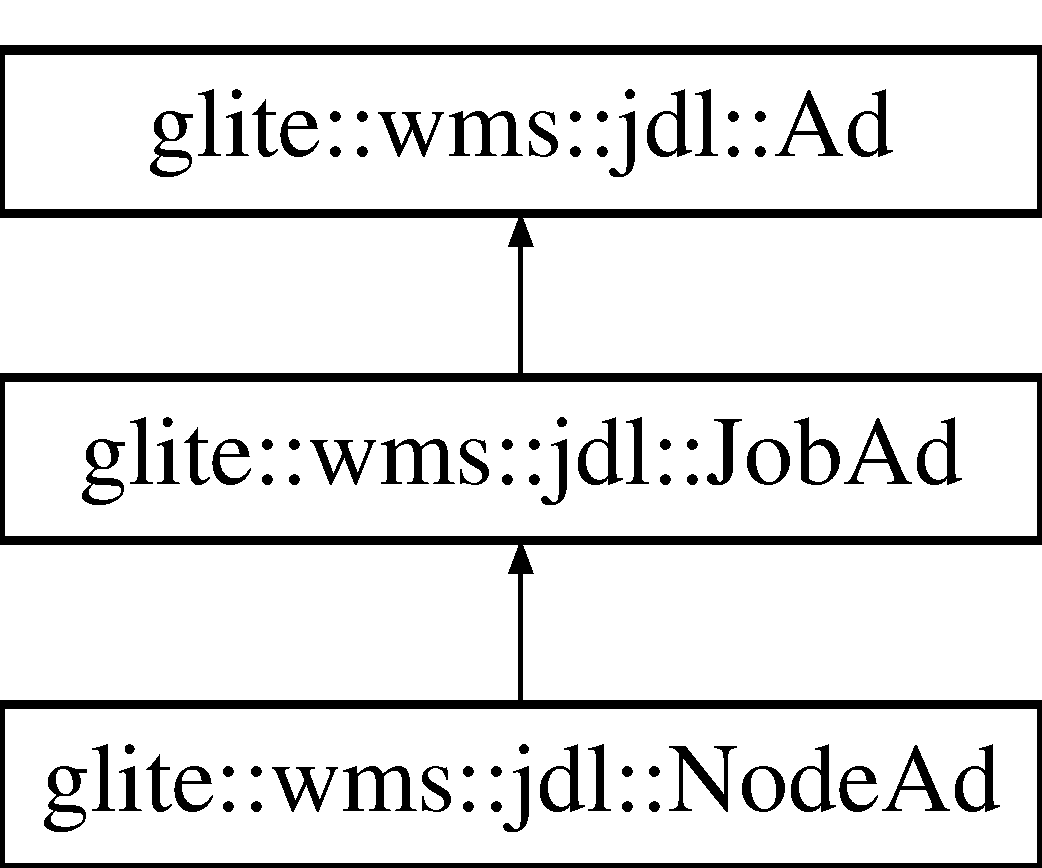
\includegraphics[height=3cm]{classglite_1_1wms_1_1jdl_1_1Ad}
\end{center}
\end{figure}
\subsection*{Get Methods}
\begin{CompactItemize}
\item 
enum \{ \par
\hyperlink{classglite_1_1wms_1_1jdl_1_1Ad_z19_0w0}{TYPE\_\-UNKNOWN} =  classad::Value::ERROR\_\-VALUE, 
\hyperlink{classglite_1_1wms_1_1jdl_1_1Ad_z19_0w1}{TYPE\_\-INTEGER} = classad::Value::INTEGER\_\-VALUE, 
\hyperlink{classglite_1_1wms_1_1jdl_1_1Ad_z19_0w2}{TYPE\_\-BOOLEAN} = classad::Value::BOOLEAN\_\-VALUE, 
\hyperlink{classglite_1_1wms_1_1jdl_1_1Ad_z19_0w3}{TYPE\_\-STRING} = classad::Value::STRING\_\-VALUE, 
\par
\hyperlink{classglite_1_1wms_1_1jdl_1_1Ad_z19_0w4}{TYPE\_\-REAL} = classad::Value::REAL\_\-VALUE, 
\hyperlink{classglite_1_1wms_1_1jdl_1_1Ad_z19_0w5}{TYPE\_\-EXPRESSION} = classad::Value::UNDEFINED\_\-VALUE
 \}
\item 
int \hyperlink{classglite_1_1wms_1_1jdl_1_1Ad_z19_1}{get\-Type} (const std::string \&attr\_\-name)
\item 
void \hyperlink{classglite_1_1wms_1_1jdl_1_1Ad_z19_2}{add\-Attribute} (const std::string \&attr\_\-name, int attr\_\-value)
\item 
void \hyperlink{classglite_1_1wms_1_1jdl_1_1Ad_z19_3}{add\-Attribute} (const std::string \&attr\_\-name, double attr\_\-value)
\item 
void \hyperlink{classglite_1_1wms_1_1jdl_1_1Ad_z19_4}{add\-Attribute} (const std::string \&attr\_\-name, bool attr\_\-value)
\item 
void \hyperlink{classglite_1_1wms_1_1jdl_1_1Ad_z19_5}{add\-Attribute} (const std::string \&attr\_\-name, const std::string \&attr\_\-value)
\item 
void \hyperlink{classglite_1_1wms_1_1jdl_1_1Ad_z19_6}{add\-Attribute} (const std::string \&attr\_\-name, const char $\ast$attr\_\-value)
\item 
void \hyperlink{classglite_1_1wms_1_1jdl_1_1Ad_z19_7}{add\-Attribute} (const std::string \&attr\_\-name, \hyperlink{classglite_1_1wms_1_1jdl_1_1Ad}{Ad} $\ast$attr\_\-value)
\item 
virtual void \hyperlink{classglite_1_1wms_1_1jdl_1_1Ad_z19_8}{set\-Attribute\-Expr} (const std::string \&attr\_\-name, const std::string \&attr\_\-value)
\item 
virtual void \hyperlink{classglite_1_1wms_1_1jdl_1_1Ad_z19_9}{set\-Attribute} (const std::string \&attr\_\-name, int attr\_\-value)
\item 
virtual void \hyperlink{classglite_1_1wms_1_1jdl_1_1Ad_z19_10}{set\-Attribute} (const std::string \&attr\_\-name, const std::string \&attr\_\-value)
\item 
virtual void \hyperlink{classglite_1_1wms_1_1jdl_1_1Ad_z19_11}{set\-Attribute} (const std::string \&attr\_\-name, const char $\ast$attr\_\-value)
\item 
virtual void \hyperlink{classglite_1_1wms_1_1jdl_1_1Ad_z19_12}{set\-Attribute} (const std::string \&attr\_\-name, double attr\_\-value)
\item 
virtual void \hyperlink{classglite_1_1wms_1_1jdl_1_1Ad_z19_13}{set\-Attribute} (const std::string \&attr\_\-name, bool attr\_\-value)
\item 
virtual void \hyperlink{classglite_1_1wms_1_1jdl_1_1Ad_z19_14}{set\-Attribute} (const std::string \&attr\_\-name, \hyperlink{classglite_1_1wms_1_1jdl_1_1Ad}{Ad} $\ast$attr\_\-value)
\item 
virtual void \hyperlink{classglite_1_1wms_1_1jdl_1_1Ad_z19_15}{set\-Attribute\-Expr} (const std::string \&attr\_\-name, classad::Expr\-Tree $\ast$attr\_\-value)
\item 
virtual std::string \hyperlink{classglite_1_1wms_1_1jdl_1_1Ad_z19_16}{get\-Attribute\-Expr} (const std::string \&attr\_\-name)
\item 
std::vector$<$ int $>$ \hyperlink{classglite_1_1wms_1_1jdl_1_1Ad_z19_17}{get\-Int\-Value} (const std::string \&attr\_\-name)
\item 
std::vector$<$ double $>$ \hyperlink{classglite_1_1wms_1_1jdl_1_1Ad_z19_18}{get\-Double\-Value} (const std::string \&attr\_\-name)
\item 
std::vector$<$ bool $>$ \hyperlink{classglite_1_1wms_1_1jdl_1_1Ad_z19_19}{get\-Bool\-Value} (const std::string \&attr\_\-name)
\item 
std::vector$<$ std::string $>$ \hyperlink{classglite_1_1wms_1_1jdl_1_1Ad_z19_20}{get\-String\-Value} (const std::string \&attr\_\-name)
\item 
std::vector$<$ std::vector$<$ std::string $>$ $>$ \hyperlink{classglite_1_1wms_1_1jdl_1_1Ad_z19_21}{get\-String\-List} (const std::string \&attr\_\-name)
\end{CompactItemize}
\subsection*{Public Types}
\subsection*{Public Member Functions}
\begin{Indent}{\bf Constructors}\par
\begin{CompactItemize}
\item 
\hyperlink{classglite_1_1wms_1_1jdl_1_1Ad_z11_0}{Ad} ()
\item 
virtual \hyperlink{classglite_1_1wms_1_1jdl_1_1Ad_z11_1}{$\sim$Ad} ()  throw ()
\item 
\hyperlink{classglite_1_1wms_1_1jdl_1_1Ad_z11_2}{Ad} (const classad::Class\-Ad \&class\-Ad)
\item 
\hyperlink{classglite_1_1wms_1_1jdl_1_1Ad_z11_3}{Ad} (const std::string \&jdl\_\-string)
\item 
classad::Class\-Ad $\ast$ \hyperlink{classglite_1_1wms_1_1jdl_1_1Ad_z11_4}{ad} ()
\end{CompactItemize}
\end{Indent}
\begin{Indent}{\bf From methods}\par
\begin{CompactItemize}
\item 
virtual void \hyperlink{classglite_1_1wms_1_1jdl_1_1Ad_z13_0}{from\-String} (const std::string \&jdl\_\-string)
\item 
virtual void \hyperlink{classglite_1_1wms_1_1jdl_1_1Ad_z13_1}{from\-File} (const std::string \&jdl\_\-file)
\end{CompactItemize}
\end{Indent}
\begin{Indent}{\bf To methods}\par
\begin{CompactItemize}
\item 
virtual std::string \hyperlink{classglite_1_1wms_1_1jdl_1_1Ad_z15_0}{to\-String} ()
\item 
virtual std::string \hyperlink{classglite_1_1wms_1_1jdl_1_1Ad_z15_1}{to\-String} (const std::string \&attr\_\-name)
\item 
virtual std::string \hyperlink{classglite_1_1wms_1_1jdl_1_1Ad_z15_2}{to\-Lines} ()
\item 
bool \hyperlink{classglite_1_1wms_1_1jdl_1_1Ad_z15_3}{is\-Set} ()
\item 
void \hyperlink{classglite_1_1wms_1_1jdl_1_1Ad_z15_4}{clear} ()
\end{CompactItemize}
\end{Indent}
\begin{Indent}{\bf has methods}\par
\begin{CompactItemize}
\item 
bool \hyperlink{classglite_1_1wms_1_1jdl_1_1Ad_z17_0}{has\-Attribute} (const std::string \&attr\_\-name)
\item 
virtual classad::Expr\-Tree $\ast$ \hyperlink{classglite_1_1wms_1_1jdl_1_1Ad_z17_1}{del\-Attribute} (const std::string \&attr\_\-name)
\item 
bool \hyperlink{classglite_1_1wms_1_1jdl_1_1Ad_z17_2}{has\-Attribute} (const std::string \&attr\_\-name, const std::string \&attr\_\-value)
\item 
std::vector$<$ std::string $>$ \hyperlink{classglite_1_1wms_1_1jdl_1_1Ad_z17_3}{attributes} ()
\end{CompactItemize}
\end{Indent}
\subsection*{Protected Member Functions}
\begin{CompactItemize}
\item 
virtual void \hyperlink{classglite_1_1wms_1_1jdl_1_1Ad_b0}{add\-Attribute} (std::string attr\_\-name, classad::Value val)
\item 
virtual void \hyperlink{classglite_1_1wms_1_1jdl_1_1Ad_b1}{append\-Value} (classad::Expr\-Tree $\ast$tree, const classad::Value \&val, const std::string \&attr\_\-name)
\item 
virtual void \hyperlink{classglite_1_1wms_1_1jdl_1_1Ad_b2}{insert\-Attribute} (const std::string \&attr\_\-name, classad::Expr\-Tree $\ast$val)
\item 
virtual void \hyperlink{classglite_1_1wms_1_1jdl_1_1Ad_b3}{insert\-Attribute} (const std::string \&attr\_\-name, classad::Value val)
\item 
virtual classad::Value \hyperlink{classglite_1_1wms_1_1jdl_1_1Ad_b4}{get\-Type\-Value} (const std::string \&attr\_\-name)
\item 
bool \hyperlink{classglite_1_1wms_1_1jdl_1_1Ad_b5}{has\-Attribute} (classad::Expr\-Tree $\ast$tree, const std::string \&attr\_\-value)
\end{CompactItemize}


\subsection{Detailed Description}
Provides a common interface for all \hyperlink{classglite_1_1wms_1_1jdl_1_1Ad}{Ad} components. It allows the user to create a valid Class\-Ad instance utilizing native classes and retrieve any kind of information from it. It is utilised as a superclass for \hyperlink{classglite_1_1wms_1_1jdl_1_1JobAd}{Job\-Ad} class \begin{Desc}
\item[See also:]Joib\-Ad\end{Desc}
\begin{Desc}
\item[Version:]0.1 \end{Desc}
\begin{Desc}
\item[Date:]15 April 2002 \end{Desc}
\begin{Desc}
\item[Author:]Alessandro Maraschini $<$\href{mailto:alessandro.maraschini@datamat.it}{\tt alessandro.maraschini@datamat.it}$>$ \end{Desc}




\subsection{Member Enumeration Documentation}
\hypertarget{classglite_1_1wms_1_1jdl_1_1Ad_z19_0}{
\subsubsection["@0]{\setlength{\rightskip}{0pt plus 5cm}anonymous enum}}
\label{classglite_1_1wms_1_1jdl_1_1Ad_z19_0}


\begin{Desc}
\item[Enumeration values: ]\par
\begin{description}
\index{TYPE_UNKNOWN@{TYPE\_\-UNKNOWN}!glite::wms::jdl::Ad@{glite::wms::jdl::Ad}}\index{glite::wms::jdl::Ad@{glite::wms::jdl::Ad}!TYPE_UNKNOWN@{TYPE\_\-UNKNOWN}}\item[{\em 
\hypertarget{classglite_1_1wms_1_1jdl_1_1Ad_z19_0w0}{
TYPE\_\-UNKNOWN}
\label{classglite_1_1wms_1_1jdl_1_1Ad_z19_0w0}
}]Unknown type \begin{Desc}
\item[See also:]\hyperlink{classglite_1_1wms_1_1jdl_1_1Ad_z19_1}{get\-Type} \end{Desc}
\index{TYPE_INTEGER@{TYPE\_\-INTEGER}!glite::wms::jdl::Ad@{glite::wms::jdl::Ad}}\index{glite::wms::jdl::Ad@{glite::wms::jdl::Ad}!TYPE_INTEGER@{TYPE\_\-INTEGER}}\item[{\em 
\hypertarget{classglite_1_1wms_1_1jdl_1_1Ad_z19_0w1}{
TYPE\_\-INTEGER}
\label{classglite_1_1wms_1_1jdl_1_1Ad_z19_0w1}
}]Attribute Integer type value \begin{Desc}
\item[See also:]\hyperlink{classglite_1_1wms_1_1jdl_1_1Ad_z19_1}{get\-Type} \end{Desc}
\index{TYPE_BOOLEAN@{TYPE\_\-BOOLEAN}!glite::wms::jdl::Ad@{glite::wms::jdl::Ad}}\index{glite::wms::jdl::Ad@{glite::wms::jdl::Ad}!TYPE_BOOLEAN@{TYPE\_\-BOOLEAN}}\item[{\em 
\hypertarget{classglite_1_1wms_1_1jdl_1_1Ad_z19_0w2}{
TYPE\_\-BOOLEAN}
\label{classglite_1_1wms_1_1jdl_1_1Ad_z19_0w2}
}]Attribute Boolean type value \begin{Desc}
\item[See also:]\hyperlink{classglite_1_1wms_1_1jdl_1_1Ad_z19_1}{get\-Type} \end{Desc}
\index{TYPE_STRING@{TYPE\_\-STRING}!glite::wms::jdl::Ad@{glite::wms::jdl::Ad}}\index{glite::wms::jdl::Ad@{glite::wms::jdl::Ad}!TYPE_STRING@{TYPE\_\-STRING}}\item[{\em 
\hypertarget{classglite_1_1wms_1_1jdl_1_1Ad_z19_0w3}{
TYPE\_\-STRING}
\label{classglite_1_1wms_1_1jdl_1_1Ad_z19_0w3}
}]Attribute String type value \begin{Desc}
\item[See also:]\hyperlink{classglite_1_1wms_1_1jdl_1_1Ad_z19_1}{get\-Type} \end{Desc}
\index{TYPE_REAL@{TYPE\_\-REAL}!glite::wms::jdl::Ad@{glite::wms::jdl::Ad}}\index{glite::wms::jdl::Ad@{glite::wms::jdl::Ad}!TYPE_REAL@{TYPE\_\-REAL}}\item[{\em 
\hypertarget{classglite_1_1wms_1_1jdl_1_1Ad_z19_0w4}{
TYPE\_\-REAL}
\label{classglite_1_1wms_1_1jdl_1_1Ad_z19_0w4}
}]Attribute Real/Double type value \begin{Desc}
\item[See also:]\hyperlink{classglite_1_1wms_1_1jdl_1_1Ad_z19_1}{get\-Type} \end{Desc}
\index{TYPE_EXPRESSION@{TYPE\_\-EXPRESSION}!glite::wms::jdl::Ad@{glite::wms::jdl::Ad}}\index{glite::wms::jdl::Ad@{glite::wms::jdl::Ad}!TYPE_EXPRESSION@{TYPE\_\-EXPRESSION}}\item[{\em 
\hypertarget{classglite_1_1wms_1_1jdl_1_1Ad_z19_0w5}{
TYPE\_\-EXPRESSION}
\label{classglite_1_1wms_1_1jdl_1_1Ad_z19_0w5}
}]Attribute Expression type value \begin{Desc}
\item[See also:]\hyperlink{classglite_1_1wms_1_1jdl_1_1Ad_z19_1}{get\-Type} \end{Desc}
\end{description}
\end{Desc}



\subsection{Constructor \& Destructor Documentation}
\hypertarget{classglite_1_1wms_1_1jdl_1_1Ad_z11_0}{
\index{glite::wms::jdl::Ad@{glite::wms::jdl::Ad}!Ad@{Ad}}
\index{Ad@{Ad}!glite::wms::jdl::Ad@{glite::wms::jdl::Ad}}
\subsubsection[Ad]{\setlength{\rightskip}{0pt plus 5cm}glite::wms::jdl::Ad::Ad ()}}
\label{classglite_1_1wms_1_1jdl_1_1Ad_z11_0}


default Constructor \hypertarget{classglite_1_1wms_1_1jdl_1_1Ad_z11_1}{
\index{glite::wms::jdl::Ad@{glite::wms::jdl::Ad}!~Ad@{$\sim$Ad}}
\index{~Ad@{$\sim$Ad}!glite::wms::jdl::Ad@{glite::wms::jdl::Ad}}
\subsubsection[$\sim$Ad]{\setlength{\rightskip}{0pt plus 5cm}virtual glite::wms::jdl::Ad::$\sim$\hyperlink{classglite_1_1wms_1_1jdl_1_1Ad}{Ad} ()  throw ()\hspace{0.3cm}{\tt  \mbox{[}virtual\mbox{]}}}}
\label{classglite_1_1wms_1_1jdl_1_1Ad_z11_1}


Default Destructor \hypertarget{classglite_1_1wms_1_1jdl_1_1Ad_z11_2}{
\index{glite::wms::jdl::Ad@{glite::wms::jdl::Ad}!Ad@{Ad}}
\index{Ad@{Ad}!glite::wms::jdl::Ad@{glite::wms::jdl::Ad}}
\subsubsection[Ad]{\setlength{\rightskip}{0pt plus 5cm}glite::wms::jdl::Ad::Ad (const classad::Class\-Ad \& {\em class\-Ad})}}
\label{classglite_1_1wms_1_1jdl_1_1Ad_z11_2}


Constructor by Class\-Ad \begin{Desc}
\item[Parameters:]
\begin{description}
\item[{\em class\-Ad}]the classad source where to create the \hyperlink{classglite_1_1wms_1_1jdl_1_1Ad}{Ad} instance from \end{description}
\end{Desc}
\hypertarget{classglite_1_1wms_1_1jdl_1_1Ad_z11_3}{
\index{glite::wms::jdl::Ad@{glite::wms::jdl::Ad}!Ad@{Ad}}
\index{Ad@{Ad}!glite::wms::jdl::Ad@{glite::wms::jdl::Ad}}
\subsubsection[Ad]{\setlength{\rightskip}{0pt plus 5cm}glite::wms::jdl::Ad::Ad (const std::string \& {\em jdl\_\-string})}}
\label{classglite_1_1wms_1_1jdl_1_1Ad_z11_3}


Constructor by string \begin{Desc}
\item[Parameters:]
\begin{description}
\item[{\em jdl\_\-string}]the \hyperlink{classglite_1_1wms_1_1jdl_1_1Ad}{Ad} string representation \end{description}
\end{Desc}


\subsection{Member Function Documentation}
\hypertarget{classglite_1_1wms_1_1jdl_1_1Ad_z11_4}{
\index{glite::wms::jdl::Ad@{glite::wms::jdl::Ad}!ad@{ad}}
\index{ad@{ad}!glite::wms::jdl::Ad@{glite::wms::jdl::Ad}}
\subsubsection[ad]{\setlength{\rightskip}{0pt plus 5cm}classad::Class\-Ad$\ast$ glite::wms::jdl::Ad::ad ()\hspace{0.3cm}{\tt  \mbox{[}inline\mbox{]}}}}
\label{classglite_1_1wms_1_1jdl_1_1Ad_z11_4}


Deep copy of \hyperlink{classglite_1_1wms_1_1jdl_1_1Ad}{Ad}. \begin{Desc}
\item[Returns:]a Class\-Ad pointer representing a copy of all \hyperlink{classglite_1_1wms_1_1jdl_1_1Ad}{Ad} attributes$\ast$ \end{Desc}
\hypertarget{classglite_1_1wms_1_1jdl_1_1Ad_b0}{
\index{glite::wms::jdl::Ad@{glite::wms::jdl::Ad}!addAttribute@{addAttribute}}
\index{addAttribute@{addAttribute}!glite::wms::jdl::Ad@{glite::wms::jdl::Ad}}
\subsubsection[addAttribute]{\setlength{\rightskip}{0pt plus 5cm}virtual void glite::wms::jdl::Ad::add\-Attribute (std::string {\em attr\_\-name}, classad::Value {\em val})\hspace{0.3cm}{\tt  \mbox{[}protected, virtual\mbox{]}}}}
\label{classglite_1_1wms_1_1jdl_1_1Ad_b0}


Add a value to a list (if already present) or set the first value of this attribute \begin{Desc}
\item[Parameters:]
\begin{description}
\item[{\em attr\_\-name}]a string representing the attribute name \item[{\em val}]The value of the attribute to be added \end{description}
\end{Desc}
\begin{Desc}
\item[Exceptions:]
\begin{description}
\item[{\em Ad\-Mismatch\-Exception}]The type of value is not allowed for the specified attribute name \item[{\em Ad\-Format\-Exception}]The type of value is not allowed for the specified attribute name\end{description}
\end{Desc}
\hypertarget{classglite_1_1wms_1_1jdl_1_1Ad_z19_7}{
\index{glite::wms::jdl::Ad@{glite::wms::jdl::Ad}!addAttribute@{addAttribute}}
\index{addAttribute@{addAttribute}!glite::wms::jdl::Ad@{glite::wms::jdl::Ad}}
\subsubsection[addAttribute]{\setlength{\rightskip}{0pt plus 5cm}void glite::wms::jdl::Ad::add\-Attribute (const std::string \& {\em attr\_\-name}, \hyperlink{classglite_1_1wms_1_1jdl_1_1Ad}{Ad} $\ast$ {\em attr\_\-value})}}
\label{classglite_1_1wms_1_1jdl_1_1Ad_z19_7}


Allow adding a value to an already set attribute of the \hyperlink{classglite_1_1wms_1_1jdl_1_1JobAd}{Job\-Ad} instance (i.e. it transforms it in a list attribute). if used on a non-set attribute the corresponding set\-Attribute method is automatically called. \begin{Desc}
\item[Parameters:]
\begin{description}
\item[{\em attr\_\-name}]a string representing the attribute name \item[{\em attr\_\-value}]- The value of the attribute to be added \end{description}
\end{Desc}
\begin{Desc}
\item[Exceptions:]
\begin{description}
\item[{\em Ad\-Mismatch\-Exception}]- The type of value is not allowed for the specified attribute name \item[{\em Ad\-Format\-Exception}]The type of value is not allowed for the specified attribute name \item[{\em Ad\-Syntax\-Exception}]- Syntax error caught while trying to add the attribute \end{description}
\end{Desc}
\hypertarget{classglite_1_1wms_1_1jdl_1_1Ad_z19_6}{
\index{glite::wms::jdl::Ad@{glite::wms::jdl::Ad}!addAttribute@{addAttribute}}
\index{addAttribute@{addAttribute}!glite::wms::jdl::Ad@{glite::wms::jdl::Ad}}
\subsubsection[addAttribute]{\setlength{\rightskip}{0pt plus 5cm}void glite::wms::jdl::Ad::add\-Attribute (const std::string \& {\em attr\_\-name}, const char $\ast$ {\em attr\_\-value})\hspace{0.3cm}{\tt  \mbox{[}inline\mbox{]}}}}
\label{classglite_1_1wms_1_1jdl_1_1Ad_z19_6}


Allow adding a value to an already set attribute of the \hyperlink{classglite_1_1wms_1_1jdl_1_1Ad}{Ad} instance (i.e. it transforms it in a list attribute). if used on a non-set attribute the corresponding set\-Attribute method is automatically called. \begin{Desc}
\item[Parameters:]
\begin{description}
\item[{\em attr\_\-name}]a string representing the attribute name \item[{\em attr\_\-value}]- The value of the attribute to be added \end{description}
\end{Desc}
\begin{Desc}
\item[Exceptions:]
\begin{description}
\item[{\em Ad\-Mismatch\-Exception}]- The type of value is not allowed for the specified attribute name \item[{\em Ad\-Format\-Exception}]The type of value is not allowed for the specified attribute name \item[{\em Ad\-Syntax\-Exception}]- Syntax error caught while trying to add the attribute \end{description}
\end{Desc}
\hypertarget{classglite_1_1wms_1_1jdl_1_1Ad_z19_5}{
\index{glite::wms::jdl::Ad@{glite::wms::jdl::Ad}!addAttribute@{addAttribute}}
\index{addAttribute@{addAttribute}!glite::wms::jdl::Ad@{glite::wms::jdl::Ad}}
\subsubsection[addAttribute]{\setlength{\rightskip}{0pt plus 5cm}void glite::wms::jdl::Ad::add\-Attribute (const std::string \& {\em attr\_\-name}, const std::string \& {\em attr\_\-value})}}
\label{classglite_1_1wms_1_1jdl_1_1Ad_z19_5}


Allow adding a value to an already set attribute of the \hyperlink{classglite_1_1wms_1_1jdl_1_1Ad}{Ad} instance (i.e. it transforms it in a list attribute). if used on a non-set attribute the corresponding set\-Attribute method is automatically called. \begin{Desc}
\item[Parameters:]
\begin{description}
\item[{\em attr\_\-name}]a string representing the attribute name \item[{\em attr\_\-value}]- The value of the attribute to be added \end{description}
\end{Desc}
\begin{Desc}
\item[Exceptions:]
\begin{description}
\item[{\em Ad\-Mismatch\-Exception}]- The type of value is not allowed for the specified attribute name \item[{\em Ad\-Format\-Exception}]The type of value is not allowed for the specified attribute name \item[{\em Ad\-Syntax\-Exception}]- Syntax error caught while trying to add the attribute \end{description}
\end{Desc}
\hypertarget{classglite_1_1wms_1_1jdl_1_1Ad_z19_4}{
\index{glite::wms::jdl::Ad@{glite::wms::jdl::Ad}!addAttribute@{addAttribute}}
\index{addAttribute@{addAttribute}!glite::wms::jdl::Ad@{glite::wms::jdl::Ad}}
\subsubsection[addAttribute]{\setlength{\rightskip}{0pt plus 5cm}void glite::wms::jdl::Ad::add\-Attribute (const std::string \& {\em attr\_\-name}, bool {\em attr\_\-value})}}
\label{classglite_1_1wms_1_1jdl_1_1Ad_z19_4}


Allow adding a value to an already set attribute of the \hyperlink{classglite_1_1wms_1_1jdl_1_1JobAd}{Job\-Ad} instance (i.e. it transforms it in a list attribute). if used on a non-set attribute the corresponding set\-Attribute method is automatically called. \begin{Desc}
\item[Parameters:]
\begin{description}
\item[{\em attr\_\-name}]a string representing the attribute name \item[{\em attr\_\-value}]- The value of the attribute to be added \end{description}
\end{Desc}
\begin{Desc}
\item[Exceptions:]
\begin{description}
\item[{\em Ad\-Mismatch\-Exception}]- The type of value is not allowed for the specified attribute name \item[{\em Ad\-Syntax\-Exception}]- Syntax error caught while trying to add the attribute \end{description}
\end{Desc}
\hypertarget{classglite_1_1wms_1_1jdl_1_1Ad_z19_3}{
\index{glite::wms::jdl::Ad@{glite::wms::jdl::Ad}!addAttribute@{addAttribute}}
\index{addAttribute@{addAttribute}!glite::wms::jdl::Ad@{glite::wms::jdl::Ad}}
\subsubsection[addAttribute]{\setlength{\rightskip}{0pt plus 5cm}void glite::wms::jdl::Ad::add\-Attribute (const std::string \& {\em attr\_\-name}, double {\em attr\_\-value})}}
\label{classglite_1_1wms_1_1jdl_1_1Ad_z19_3}


Allow adding a value to an already set attribute of the \hyperlink{classglite_1_1wms_1_1jdl_1_1JobAd}{Job\-Ad} instance (i.e. it transforms it in a list attribute). if used on a non-set attribute the corresponding set\-Attribute method is automatically called. \begin{Desc}
\item[Parameters:]
\begin{description}
\item[{\em attr\_\-name}]a string representing the attribute name \item[{\em attr\_\-value}]- The value of the attribute to be added \end{description}
\end{Desc}
\begin{Desc}
\item[Exceptions:]
\begin{description}
\item[{\em Ad\-Mismatch\-Exception}]- The type of value is not allowed for the specified attribute name \item[{\em Ad\-Syntax\-Exception}]- Syntax error caught while trying to add the attribute \end{description}
\end{Desc}
\hypertarget{classglite_1_1wms_1_1jdl_1_1Ad_z19_2}{
\index{glite::wms::jdl::Ad@{glite::wms::jdl::Ad}!addAttribute@{addAttribute}}
\index{addAttribute@{addAttribute}!glite::wms::jdl::Ad@{glite::wms::jdl::Ad}}
\subsubsection[addAttribute]{\setlength{\rightskip}{0pt plus 5cm}void glite::wms::jdl::Ad::add\-Attribute (const std::string \& {\em attr\_\-name}, int {\em attr\_\-value})}}
\label{classglite_1_1wms_1_1jdl_1_1Ad_z19_2}


Allow adding a value to an already set attribute of the \hyperlink{classglite_1_1wms_1_1jdl_1_1JobAd}{Job\-Ad} instance (i.e. it transforms it in a list attribute). if used on a non-set attribute the corresponding set\-Attribute method is automatically called. \begin{Desc}
\item[Parameters:]
\begin{description}
\item[{\em attr\_\-name}]a string representing the attribute name \item[{\em attr\_\-value}]- The value of the attribute to be added \end{description}
\end{Desc}
\begin{Desc}
\item[Exceptions:]
\begin{description}
\item[{\em Ad\-Mismatch\-Exception}]- The type of value is not allowed for the specified attribute name \item[{\em Ad\-Syntax\-Exception}]- Syntax error caught while trying to add the attribute \end{description}
\end{Desc}
\hypertarget{classglite_1_1wms_1_1jdl_1_1Ad_b1}{
\index{glite::wms::jdl::Ad@{glite::wms::jdl::Ad}!appendValue@{appendValue}}
\index{appendValue@{appendValue}!glite::wms::jdl::Ad@{glite::wms::jdl::Ad}}
\subsubsection[appendValue]{\setlength{\rightskip}{0pt plus 5cm}virtual void glite::wms::jdl::Ad::append\-Value (classad::Expr\-Tree $\ast$ {\em tree}, const classad::Value \& {\em val}, const std::string \& {\em attr\_\-name})\hspace{0.3cm}{\tt  \mbox{[}protected, virtual\mbox{]}}}}
\label{classglite_1_1wms_1_1jdl_1_1Ad_b1}


Append a value to a list \begin{Desc}
\item[Parameters:]
\begin{description}
\item[{\em attr\_\-name}]a string representing the attribute name \item[{\em val}]- The value of the attribute to be added \item[{\em tree}]the current value (before appending) of the attribute\end{description}
\end{Desc}
\hypertarget{classglite_1_1wms_1_1jdl_1_1Ad_z17_3}{
\index{glite::wms::jdl::Ad@{glite::wms::jdl::Ad}!attributes@{attributes}}
\index{attributes@{attributes}!glite::wms::jdl::Ad@{glite::wms::jdl::Ad}}
\subsubsection[attributes]{\setlength{\rightskip}{0pt plus 5cm}std::vector$<$std::string$>$ glite::wms::jdl::Ad::attributes ()}}
\label{classglite_1_1wms_1_1jdl_1_1Ad_z17_3}


Retrieve the list of attribugtes present inside the instance \begin{Desc}
\item[Returns:]a vector containing (with no order) all the attributes of the \hyperlink{classglite_1_1wms_1_1jdl_1_1Ad}{Ad}\end{Desc}
\hypertarget{classglite_1_1wms_1_1jdl_1_1Ad_z15_4}{
\index{glite::wms::jdl::Ad@{glite::wms::jdl::Ad}!clear@{clear}}
\index{clear@{clear}!glite::wms::jdl::Ad@{glite::wms::jdl::Ad}}
\subsubsection[clear]{\setlength{\rightskip}{0pt plus 5cm}void glite::wms::jdl::Ad::clear ()}}
\label{classglite_1_1wms_1_1jdl_1_1Ad_z15_4}


Reset the \hyperlink{classglite_1_1wms_1_1jdl_1_1JobAd}{Job\-Ad} Instance. All the previous existing attributes will be deleted \hypertarget{classglite_1_1wms_1_1jdl_1_1Ad_z17_1}{
\index{glite::wms::jdl::Ad@{glite::wms::jdl::Ad}!delAttribute@{delAttribute}}
\index{delAttribute@{delAttribute}!glite::wms::jdl::Ad@{glite::wms::jdl::Ad}}
\subsubsection[delAttribute]{\setlength{\rightskip}{0pt plus 5cm}virtual classad::Expr\-Tree$\ast$ glite::wms::jdl::Ad::del\-Attribute (const std::string \& {\em attr\_\-name})\hspace{0.3cm}{\tt  \mbox{[}virtual\mbox{]}}}}
\label{classglite_1_1wms_1_1jdl_1_1Ad_z17_1}


Delete an Attribute. It fails if the attribute doesn't exist \begin{Desc}
\item[Exceptions:]
\begin{description}
\item[{\em Ad\-Empty\-Exception}]attribute has not been set yet \end{description}
\end{Desc}
\begin{Desc}
\item[Returns:]the deep copy of the expression for the deleted attribute \end{Desc}
\begin{Desc}
\item[Parameters:]
\begin{description}
\item[{\em attr\_\-nam}]The name of the attibute to be deleted \end{description}
\end{Desc}


Reimplemented in \hyperlink{classglite_1_1wms_1_1jdl_1_1JobAd_z9_2}{glite::wms::jdl::Job\-Ad}.\hypertarget{classglite_1_1wms_1_1jdl_1_1Ad_z13_1}{
\index{glite::wms::jdl::Ad@{glite::wms::jdl::Ad}!fromFile@{fromFile}}
\index{fromFile@{fromFile}!glite::wms::jdl::Ad@{glite::wms::jdl::Ad}}
\subsubsection[fromFile]{\setlength{\rightskip}{0pt plus 5cm}virtual void glite::wms::jdl::Ad::from\-File (const std::string \& {\em jdl\_\-file})\hspace{0.3cm}{\tt  \mbox{[}virtual\mbox{]}}}}
\label{classglite_1_1wms_1_1jdl_1_1Ad_z13_1}


Create an \hyperlink{classglite_1_1wms_1_1jdl_1_1Ad}{Ad} instacne from a file \begin{Desc}
\item[Parameters:]
\begin{description}
\item[{\em jdl\_\-file}]the string representing the path containing the jdl to be parsed \end{description}
\end{Desc}
\hypertarget{classglite_1_1wms_1_1jdl_1_1Ad_z13_0}{
\index{glite::wms::jdl::Ad@{glite::wms::jdl::Ad}!fromString@{fromString}}
\index{fromString@{fromString}!glite::wms::jdl::Ad@{glite::wms::jdl::Ad}}
\subsubsection[fromString]{\setlength{\rightskip}{0pt plus 5cm}virtual void glite::wms::jdl::Ad::from\-String (const std::string \& {\em jdl\_\-string})\hspace{0.3cm}{\tt  \mbox{[}virtual\mbox{]}}}}
\label{classglite_1_1wms_1_1jdl_1_1Ad_z13_0}


Create an \hyperlink{classglite_1_1wms_1_1jdl_1_1Ad}{Ad} instance from a string \begin{Desc}
\item[Parameters:]
\begin{description}
\item[{\em jdl\_\-string}]the ad string representation \end{description}
\end{Desc}
\hypertarget{classglite_1_1wms_1_1jdl_1_1Ad_z19_16}{
\index{glite::wms::jdl::Ad@{glite::wms::jdl::Ad}!getAttributeExpr@{getAttributeExpr}}
\index{getAttributeExpr@{getAttributeExpr}!glite::wms::jdl::Ad@{glite::wms::jdl::Ad}}
\subsubsection[getAttributeExpr]{\setlength{\rightskip}{0pt plus 5cm}virtual std::string glite::wms::jdl::Ad::get\-Attribute\-Expr (const std::string \& {\em attr\_\-name})\hspace{0.3cm}{\tt  \mbox{[}virtual\mbox{]}}}}
\label{classglite_1_1wms_1_1jdl_1_1Ad_z19_16}


Retreive the value of the specified attribute \begin{Desc}
\item[Parameters:]
\begin{description}
\item[{\em attr\_\-name}]The name of the attribute name to be retrieved \end{description}
\end{Desc}
\begin{Desc}
\item[Returns:]the string representation of this attribute \end{Desc}
\begin{Desc}
\item[Exceptions:]
\begin{description}
\item[{\em Ad\-Empty\-Exception}]- The checked attribute has not been set yet \item[{\em Ad\-Mismatch\-Exception}]- The type of retrieved value is not allowed for the specified attribute name \end{description}
\end{Desc}
\hypertarget{classglite_1_1wms_1_1jdl_1_1Ad_z19_19}{
\index{glite::wms::jdl::Ad@{glite::wms::jdl::Ad}!getBoolValue@{getBoolValue}}
\index{getBoolValue@{getBoolValue}!glite::wms::jdl::Ad@{glite::wms::jdl::Ad}}
\subsubsection[getBoolValue]{\setlength{\rightskip}{0pt plus 5cm}std::vector$<$bool$>$ glite::wms::jdl::Ad::get\-Bool\-Value (const std::string \& {\em attr\_\-name})}}
\label{classglite_1_1wms_1_1jdl_1_1Ad_z19_19}


Retreive the value of the specified attribute \begin{Desc}
\item[Parameters:]
\begin{description}
\item[{\em attr\_\-name}]The name of the attribute to be retrieved \end{description}
\end{Desc}
\begin{Desc}
\item[Returns:]a vector cantaining the values listed in the specified attribute , (1-size vector if the attribute has a single value) \end{Desc}
\begin{Desc}
\item[Exceptions:]
\begin{description}
\item[{\em Ad\-Empty\-Exception}]- The checked attribute has not been set yet \item[{\em Ad\-Mismatch\-Exception}]- The type of retrieved value is not allowed for the specified attribute name \end{description}
\end{Desc}
\hypertarget{classglite_1_1wms_1_1jdl_1_1Ad_z19_18}{
\index{glite::wms::jdl::Ad@{glite::wms::jdl::Ad}!getDoubleValue@{getDoubleValue}}
\index{getDoubleValue@{getDoubleValue}!glite::wms::jdl::Ad@{glite::wms::jdl::Ad}}
\subsubsection[getDoubleValue]{\setlength{\rightskip}{0pt plus 5cm}std::vector$<$double$>$ glite::wms::jdl::Ad::get\-Double\-Value (const std::string \& {\em attr\_\-name})}}
\label{classglite_1_1wms_1_1jdl_1_1Ad_z19_18}


Retreive the value of the specified attribute \begin{Desc}
\item[Parameters:]
\begin{description}
\item[{\em attr\_\-name}]The name of the attribute to be retrieved \end{description}
\end{Desc}
\begin{Desc}
\item[Returns:]a vector cantaining the values listed in the specified attribute , (1-size vector if the attribute has a single value) \end{Desc}
\begin{Desc}
\item[Exceptions:]
\begin{description}
\item[{\em Ad\-Empty\-Exception}]- The checked attribute has not been set yet \item[{\em Ad\-Mismatch\-Exception}]- The type of retrieved value is not allowed for the specified attribute name \end{description}
\end{Desc}
\hypertarget{classglite_1_1wms_1_1jdl_1_1Ad_z19_17}{
\index{glite::wms::jdl::Ad@{glite::wms::jdl::Ad}!getIntValue@{getIntValue}}
\index{getIntValue@{getIntValue}!glite::wms::jdl::Ad@{glite::wms::jdl::Ad}}
\subsubsection[getIntValue]{\setlength{\rightskip}{0pt plus 5cm}std::vector$<$int$>$ glite::wms::jdl::Ad::get\-Int\-Value (const std::string \& {\em attr\_\-name})}}
\label{classglite_1_1wms_1_1jdl_1_1Ad_z19_17}


Retreive the value of the specified attribute \begin{Desc}
\item[Parameters:]
\begin{description}
\item[{\em attr\_\-name}]The name of the attribute name to be retrieved \end{description}
\end{Desc}
\begin{Desc}
\item[Returns:]a vector cantaining the values listed in the specified attribute , (1-size vector if the attribute has a single value) \end{Desc}
\begin{Desc}
\item[Exceptions:]
\begin{description}
\item[{\em Ad\-Empty\-Exception}]- The checked attribute has not been set yet \item[{\em Ad\-Mismatch\-Exception}]- The type of retrieved value is not allowed for the specified attribute name \end{description}
\end{Desc}
\hypertarget{classglite_1_1wms_1_1jdl_1_1Ad_z19_21}{
\index{glite::wms::jdl::Ad@{glite::wms::jdl::Ad}!getStringList@{getStringList}}
\index{getStringList@{getStringList}!glite::wms::jdl::Ad@{glite::wms::jdl::Ad}}
\subsubsection[getStringList]{\setlength{\rightskip}{0pt plus 5cm}std::vector$<$std::vector$<$std::string$>$ $>$ glite::wms::jdl::Ad::get\-String\-List (const std::string \& {\em attr\_\-name})}}
\label{classglite_1_1wms_1_1jdl_1_1Ad_z19_21}


Retreive the value of the specified attribute \begin{Desc}
\item[Parameters:]
\begin{description}
\item[{\em attr\_\-name}]The name of the attribute to be retrieved \end{description}
\end{Desc}
\begin{Desc}
\item[Returns:]a vector cantaining the a vector of strings (1-size vector if the attribute has a single value) \end{Desc}
\begin{Desc}
\item[Exceptions:]
\begin{description}
\item[{\em Ad\-Empty\-Exception}]- The checked attribute has not been set yet \item[{\em Ad\-Mismatch\-Exception}]- The type of retrieved value is not allowed for the specified attribute name \end{description}
\end{Desc}
\hypertarget{classglite_1_1wms_1_1jdl_1_1Ad_z19_20}{
\index{glite::wms::jdl::Ad@{glite::wms::jdl::Ad}!getStringValue@{getStringValue}}
\index{getStringValue@{getStringValue}!glite::wms::jdl::Ad@{glite::wms::jdl::Ad}}
\subsubsection[getStringValue]{\setlength{\rightskip}{0pt plus 5cm}std::vector$<$std::string$>$ glite::wms::jdl::Ad::get\-String\-Value (const std::string \& {\em attr\_\-name})}}
\label{classglite_1_1wms_1_1jdl_1_1Ad_z19_20}


Retreive the value of the specified attribute \begin{Desc}
\item[Parameters:]
\begin{description}
\item[{\em attr\_\-name}]The name of the attribute to be retrieved \end{description}
\end{Desc}
\begin{Desc}
\item[Returns:]a vector cantaining the values listed in the specified attribute , (1-size vector if the attribute has a single value) \end{Desc}
\begin{Desc}
\item[Exceptions:]
\begin{description}
\item[{\em Ad\-Empty\-Exception}]- The checked attribute has not been set yet \item[{\em Ad\-Mismatch\-Exception}]- The type of retrieved value is not allowed for the specified attribute name \end{description}
\end{Desc}
\hypertarget{classglite_1_1wms_1_1jdl_1_1Ad_z19_1}{
\index{glite::wms::jdl::Ad@{glite::wms::jdl::Ad}!getType@{getType}}
\index{getType@{getType}!glite::wms::jdl::Ad@{glite::wms::jdl::Ad}}
\subsubsection[getType]{\setlength{\rightskip}{0pt plus 5cm}int glite::wms::jdl::Ad::get\-Type (const std::string \& {\em attr\_\-name})}}
\label{classglite_1_1wms_1_1jdl_1_1Ad_z19_1}


Retrieve the type of the value specified for attr\_\-name \begin{Desc}
\item[Parameters:]
\begin{description}
\item[{\em attr\_\-name}]the name of the attribute \end{description}
\end{Desc}
\begin{Desc}
\item[Returns:]an integer representing the type of the attribute \end{Desc}
\begin{Desc}
\item[Exceptions:]
\begin{description}
\item[{\em Ad\-Empty\-Exception}]if the attribute is not present in the \hyperlink{classglite_1_1wms_1_1jdl_1_1JobAd}{Job\-Ad} instance \end{description}
\end{Desc}
\begin{Desc}
\item[See also:]\hyperlink{classglite_1_1wms_1_1jdl_1_1Ad_z19_0w0}{TYPE\_\-UNKNOWN} 

\hyperlink{classglite_1_1wms_1_1jdl_1_1Ad_z19_0w1}{TYPE\_\-INTEGER} 

\hyperlink{classglite_1_1wms_1_1jdl_1_1Ad_z19_0w2}{TYPE\_\-BOOLEAN} 

\hyperlink{classglite_1_1wms_1_1jdl_1_1Ad_z19_0w3}{TYPE\_\-STRING} 

\hyperlink{classglite_1_1wms_1_1jdl_1_1Ad_z19_0w4}{TYPE\_\-REAL} 

\hyperlink{classglite_1_1wms_1_1jdl_1_1Ad_z19_0w5}{TYPE\_\-EXPRESSION} \end{Desc}
\hypertarget{classglite_1_1wms_1_1jdl_1_1Ad_b4}{
\index{glite::wms::jdl::Ad@{glite::wms::jdl::Ad}!getTypeValue@{getTypeValue}}
\index{getTypeValue@{getTypeValue}!glite::wms::jdl::Ad@{glite::wms::jdl::Ad}}
\subsubsection[getTypeValue]{\setlength{\rightskip}{0pt plus 5cm}virtual classad::Value glite::wms::jdl::Ad::get\-Type\-Value (const std::string \& {\em attr\_\-name})\hspace{0.3cm}{\tt  \mbox{[}protected, virtual\mbox{]}}}}
\label{classglite_1_1wms_1_1jdl_1_1Ad_b4}


Retrieve the Value of the specified attribute \begin{Desc}
\item[Parameters:]
\begin{description}
\item[{\em attr\_\-name}]a string representing the attribute name \end{description}
\end{Desc}
\begin{Desc}
\item[Returns:]the Value of the attribute inside the \hyperlink{classglite_1_1wms_1_1jdl_1_1Ad}{Ad} instance\end{Desc}
\hypertarget{classglite_1_1wms_1_1jdl_1_1Ad_b5}{
\index{glite::wms::jdl::Ad@{glite::wms::jdl::Ad}!hasAttribute@{hasAttribute}}
\index{hasAttribute@{hasAttribute}!glite::wms::jdl::Ad@{glite::wms::jdl::Ad}}
\subsubsection[hasAttribute]{\setlength{\rightskip}{0pt plus 5cm}bool glite::wms::jdl::Ad::has\-Attribute (classad::Expr\-Tree $\ast$ {\em tree}, const std::string \& {\em attr\_\-value})\hspace{0.3cm}{\tt  \mbox{[}protected\mbox{]}}}}
\label{classglite_1_1wms_1_1jdl_1_1Ad_b5}


Check whether a value is present inside a classad Expression \begin{Desc}
\item[Parameters:]
\begin{description}
\item[{\em tree}]the expression to be checked @ attr\_\-value the value to be checked \end{description}
\end{Desc}
\begin{Desc}
\item[Returns:]true (if the value is present) false otherwise \end{Desc}
\hypertarget{classglite_1_1wms_1_1jdl_1_1Ad_z17_2}{
\index{glite::wms::jdl::Ad@{glite::wms::jdl::Ad}!hasAttribute@{hasAttribute}}
\index{hasAttribute@{hasAttribute}!glite::wms::jdl::Ad@{glite::wms::jdl::Ad}}
\subsubsection[hasAttribute]{\setlength{\rightskip}{0pt plus 5cm}bool glite::wms::jdl::Ad::has\-Attribute (const std::string \& {\em attr\_\-name}, const std::string \& {\em attr\_\-value})}}
\label{classglite_1_1wms_1_1jdl_1_1Ad_z17_2}


Check if the specified value is present in the specified attribute \hypertarget{classglite_1_1wms_1_1jdl_1_1Ad_z17_0}{
\index{glite::wms::jdl::Ad@{glite::wms::jdl::Ad}!hasAttribute@{hasAttribute}}
\index{hasAttribute@{hasAttribute}!glite::wms::jdl::Ad@{glite::wms::jdl::Ad}}
\subsubsection[hasAttribute]{\setlength{\rightskip}{0pt plus 5cm}bool glite::wms::jdl::Ad::has\-Attribute (const std::string \& {\em attr\_\-name})}}
\label{classglite_1_1wms_1_1jdl_1_1Ad_z17_0}


Check If the specified attribute has already been set \begin{Desc}
\item[Parameters:]
\begin{description}
\item[{\em attr\_\-nam}]The name of the attibute to be looked for \end{description}
\end{Desc}
\begin{Desc}
\item[Returns:]{\em true\/} if the attribute has been found, {\em false\/} otherwise \end{Desc}
\hypertarget{classglite_1_1wms_1_1jdl_1_1Ad_b3}{
\index{glite::wms::jdl::Ad@{glite::wms::jdl::Ad}!insertAttribute@{insertAttribute}}
\index{insertAttribute@{insertAttribute}!glite::wms::jdl::Ad@{glite::wms::jdl::Ad}}
\subsubsection[insertAttribute]{\setlength{\rightskip}{0pt plus 5cm}virtual void glite::wms::jdl::Ad::insert\-Attribute (const std::string \& {\em attr\_\-name}, classad::Value {\em val})\hspace{0.3cm}{\tt  \mbox{[}protected, virtual\mbox{]}}}}
\label{classglite_1_1wms_1_1jdl_1_1Ad_b3}


Insert a classad Exptression inside the \hyperlink{classglite_1_1wms_1_1jdl_1_1Ad}{Ad} instance \begin{Desc}
\item[Parameters:]
\begin{description}
\item[{\em attr\_\-name}]a string representing the attribute name \item[{\em val}]- The value of the attribute to be added\end{description}
\end{Desc}
\hypertarget{classglite_1_1wms_1_1jdl_1_1Ad_b2}{
\index{glite::wms::jdl::Ad@{glite::wms::jdl::Ad}!insertAttribute@{insertAttribute}}
\index{insertAttribute@{insertAttribute}!glite::wms::jdl::Ad@{glite::wms::jdl::Ad}}
\subsubsection[insertAttribute]{\setlength{\rightskip}{0pt plus 5cm}virtual void glite::wms::jdl::Ad::insert\-Attribute (const std::string \& {\em attr\_\-name}, classad::Expr\-Tree $\ast$ {\em val})\hspace{0.3cm}{\tt  \mbox{[}protected, virtual\mbox{]}}}}
\label{classglite_1_1wms_1_1jdl_1_1Ad_b2}


Insert a classad Exptression inside the \hyperlink{classglite_1_1wms_1_1jdl_1_1Ad}{Ad} instance \begin{Desc}
\item[Parameters:]
\begin{description}
\item[{\em attr\_\-name}]a string representing the attribute name \item[{\em val}]- The value of the attribute to be added\end{description}
\end{Desc}


Reimplemented in \hyperlink{classglite_1_1wms_1_1jdl_1_1JobAd_b2}{glite::wms::jdl::Job\-Ad}, and \hyperlink{classglite_1_1wms_1_1jdl_1_1NodeAd_b2}{glite::wms::jdl::Node\-Ad}.\hypertarget{classglite_1_1wms_1_1jdl_1_1Ad_z15_3}{
\index{glite::wms::jdl::Ad@{glite::wms::jdl::Ad}!isSet@{isSet}}
\index{isSet@{isSet}!glite::wms::jdl::Ad@{glite::wms::jdl::Ad}}
\subsubsection[isSet]{\setlength{\rightskip}{0pt plus 5cm}bool glite::wms::jdl::Ad::is\-Set ()}}
\label{classglite_1_1wms_1_1jdl_1_1Ad_z15_3}


Check whether the \hyperlink{classglite_1_1wms_1_1jdl_1_1JobAd}{Job\-Ad} has been initialised \begin{Desc}
\item[Returns:]whether the \hyperlink{classglite_1_1wms_1_1jdl_1_1JobAd}{Job\-Ad} has been initialised(true) or not (false) \end{Desc}
\hypertarget{classglite_1_1wms_1_1jdl_1_1Ad_z19_14}{
\index{glite::wms::jdl::Ad@{glite::wms::jdl::Ad}!setAttribute@{setAttribute}}
\index{setAttribute@{setAttribute}!glite::wms::jdl::Ad@{glite::wms::jdl::Ad}}
\subsubsection[setAttribute]{\setlength{\rightskip}{0pt plus 5cm}virtual void glite::wms::jdl::Ad::set\-Attribute (const std::string \& {\em attr\_\-name}, \hyperlink{classglite_1_1wms_1_1jdl_1_1Ad}{Ad} $\ast$ {\em attr\_\-value})\hspace{0.3cm}{\tt  \mbox{[}virtual\mbox{]}}}}
\label{classglite_1_1wms_1_1jdl_1_1Ad_z19_14}


Add The specified Integer Attribute to the jdl istance \begin{Desc}
\item[Parameters:]
\begin{description}
\item[{\em attr\_\-name}]- The Name of the attribute to be added \item[{\em attr\_\-value}]- The value of the attribute to be added \end{description}
\end{Desc}
\begin{Desc}
\item[Exceptions:]
\begin{description}
\item[{\em Ad\-Syntax\-Exception}]- Syntax error caught while trying to add the attribute \item[{\em Ad\-Empty\-Exception}]- The attribute attr\_\-name had been already set \end{description}
\end{Desc}
\hypertarget{classglite_1_1wms_1_1jdl_1_1Ad_z19_13}{
\index{glite::wms::jdl::Ad@{glite::wms::jdl::Ad}!setAttribute@{setAttribute}}
\index{setAttribute@{setAttribute}!glite::wms::jdl::Ad@{glite::wms::jdl::Ad}}
\subsubsection[setAttribute]{\setlength{\rightskip}{0pt plus 5cm}virtual void glite::wms::jdl::Ad::set\-Attribute (const std::string \& {\em attr\_\-name}, bool {\em attr\_\-value})\hspace{0.3cm}{\tt  \mbox{[}virtual\mbox{]}}}}
\label{classglite_1_1wms_1_1jdl_1_1Ad_z19_13}


Add The specified String Attribute to the jdl istance \begin{Desc}
\item[Parameters:]
\begin{description}
\item[{\em attr\_\-name}]- The Name of the attribute to be added \item[{\em attr\_\-value}]- The value of the attribute to be added \end{description}
\end{Desc}
\begin{Desc}
\item[Exceptions:]
\begin{description}
\item[{\em Ad\-Syntax\-Exception}]- Syntax error caught while trying to add the attribute \item[{\em Ad\-Empty\-Exception}]- The attribute attr\_\-name had been already set \end{description}
\end{Desc}
\hypertarget{classglite_1_1wms_1_1jdl_1_1Ad_z19_12}{
\index{glite::wms::jdl::Ad@{glite::wms::jdl::Ad}!setAttribute@{setAttribute}}
\index{setAttribute@{setAttribute}!glite::wms::jdl::Ad@{glite::wms::jdl::Ad}}
\subsubsection[setAttribute]{\setlength{\rightskip}{0pt plus 5cm}virtual void glite::wms::jdl::Ad::set\-Attribute (const std::string \& {\em attr\_\-name}, double {\em attr\_\-value})\hspace{0.3cm}{\tt  \mbox{[}virtual\mbox{]}}}}
\label{classglite_1_1wms_1_1jdl_1_1Ad_z19_12}


Add The specified String Attribute to the jdl istance \begin{Desc}
\item[Parameters:]
\begin{description}
\item[{\em attr\_\-name}]- The Name of the attribute to be added \item[{\em attr\_\-value}]- The value of the attribute to be added \end{description}
\end{Desc}
\begin{Desc}
\item[Exceptions:]
\begin{description}
\item[{\em Ad\-Syntax\-Exception}]- Syntax error caught while trying to add the attribute \item[{\em Ad\-Empty\-Exception}]- The attribute attr\_\-name had been already set \end{description}
\end{Desc}
\hypertarget{classglite_1_1wms_1_1jdl_1_1Ad_z19_11}{
\index{glite::wms::jdl::Ad@{glite::wms::jdl::Ad}!setAttribute@{setAttribute}}
\index{setAttribute@{setAttribute}!glite::wms::jdl::Ad@{glite::wms::jdl::Ad}}
\subsubsection[setAttribute]{\setlength{\rightskip}{0pt plus 5cm}virtual void glite::wms::jdl::Ad::set\-Attribute (const std::string \& {\em attr\_\-name}, const char $\ast$ {\em attr\_\-value})\hspace{0.3cm}{\tt  \mbox{[}inline, virtual\mbox{]}}}}
\label{classglite_1_1wms_1_1jdl_1_1Ad_z19_11}


Add The specified String Attribute to the jdl istance \begin{Desc}
\item[Parameters:]
\begin{description}
\item[{\em attr\_\-name}]- The Name of the attribute to be added \item[{\em attr\_\-value}]- The value of the attribute to be added \end{description}
\end{Desc}
\begin{Desc}
\item[Exceptions:]
\begin{description}
\item[{\em Ad\-Empty\-Exception}]- The attribute attr\_\-name had been already set \item[{\em Ad\-Format\-Exception}]The type of value is not allowed for the specified attribute name \end{description}
\end{Desc}
\hypertarget{classglite_1_1wms_1_1jdl_1_1Ad_z19_10}{
\index{glite::wms::jdl::Ad@{glite::wms::jdl::Ad}!setAttribute@{setAttribute}}
\index{setAttribute@{setAttribute}!glite::wms::jdl::Ad@{glite::wms::jdl::Ad}}
\subsubsection[setAttribute]{\setlength{\rightskip}{0pt plus 5cm}virtual void glite::wms::jdl::Ad::set\-Attribute (const std::string \& {\em attr\_\-name}, const std::string \& {\em attr\_\-value})\hspace{0.3cm}{\tt  \mbox{[}virtual\mbox{]}}}}
\label{classglite_1_1wms_1_1jdl_1_1Ad_z19_10}


Add The specified String Attribute to the jdl istance \begin{Desc}
\item[Parameters:]
\begin{description}
\item[{\em attr\_\-name}]- The Name of the attribute to be added \item[{\em attr\_\-value}]- The value of the attribute to be added \end{description}
\end{Desc}
\begin{Desc}
\item[Exceptions:]
\begin{description}
\item[{\em Ad\-Empty\-Exception}]- The attribute attr\_\-name had been already set \item[{\em Ad\-Format\-Exception}]The type of value is not allowed for the specified attribute name \end{description}
\end{Desc}
\hypertarget{classglite_1_1wms_1_1jdl_1_1Ad_z19_9}{
\index{glite::wms::jdl::Ad@{glite::wms::jdl::Ad}!setAttribute@{setAttribute}}
\index{setAttribute@{setAttribute}!glite::wms::jdl::Ad@{glite::wms::jdl::Ad}}
\subsubsection[setAttribute]{\setlength{\rightskip}{0pt plus 5cm}virtual void glite::wms::jdl::Ad::set\-Attribute (const std::string \& {\em attr\_\-name}, int {\em attr\_\-value})\hspace{0.3cm}{\tt  \mbox{[}virtual\mbox{]}}}}
\label{classglite_1_1wms_1_1jdl_1_1Ad_z19_9}


Add The specified Integer Attribute to the jdl istance \begin{Desc}
\item[Parameters:]
\begin{description}
\item[{\em attr\_\-name}]- The Name of the attribute to be added \item[{\em attr\_\-value}]- The value of the attribute to be added \end{description}
\end{Desc}
\begin{Desc}
\item[Exceptions:]
\begin{description}
\item[{\em Ad\-Syntax\-Exception}]- Syntax error caught while trying to add the attribute \item[{\em Ad\-Empty\-Exception}]- The attribute attr\_\-name had been already set \end{description}
\end{Desc}
\hypertarget{classglite_1_1wms_1_1jdl_1_1Ad_z19_15}{
\index{glite::wms::jdl::Ad@{glite::wms::jdl::Ad}!setAttributeExpr@{setAttributeExpr}}
\index{setAttributeExpr@{setAttributeExpr}!glite::wms::jdl::Ad@{glite::wms::jdl::Ad}}
\subsubsection[setAttributeExpr]{\setlength{\rightskip}{0pt plus 5cm}virtual void glite::wms::jdl::Ad::set\-Attribute\-Expr (const std::string \& {\em attr\_\-name}, classad::Expr\-Tree $\ast$ {\em attr\_\-value})\hspace{0.3cm}{\tt  \mbox{[}virtual\mbox{]}}}}
\label{classglite_1_1wms_1_1jdl_1_1Ad_z19_15}


Add The specified Expression Attribute to the jdl istance \begin{Desc}
\item[Parameters:]
\begin{description}
\item[{\em attr\_\-name}]- The Name of the attribute to be added \item[{\em attr\_\-value}]- The value of the attribute to be added \end{description}
\end{Desc}
\begin{Desc}
\item[Exceptions:]
\begin{description}
\item[{\em Ad\-Syntax\-Exception}]- Syntax error caught while trying to add the attribute \item[{\em Ad\-Empty\-Exception}]- The attribute attr\_\-name had been already set \end{description}
\end{Desc}


Reimplemented in \hyperlink{classglite_1_1wms_1_1jdl_1_1JobAd_z5_5}{glite::wms::jdl::Job\-Ad}.\hypertarget{classglite_1_1wms_1_1jdl_1_1Ad_z19_8}{
\index{glite::wms::jdl::Ad@{glite::wms::jdl::Ad}!setAttributeExpr@{setAttributeExpr}}
\index{setAttributeExpr@{setAttributeExpr}!glite::wms::jdl::Ad@{glite::wms::jdl::Ad}}
\subsubsection[setAttributeExpr]{\setlength{\rightskip}{0pt plus 5cm}virtual void glite::wms::jdl::Ad::set\-Attribute\-Expr (const std::string \& {\em attr\_\-name}, const std::string \& {\em attr\_\-value})\hspace{0.3cm}{\tt  \mbox{[}virtual\mbox{]}}}}
\label{classglite_1_1wms_1_1jdl_1_1Ad_z19_8}


Add The specified Expression Attribute to the jdl istance \begin{Desc}
\item[Parameters:]
\begin{description}
\item[{\em attr\_\-name}]- The Name of the attribute to be added \item[{\em attr\_\-value}]- The string expression of the attribute to be added \end{description}
\end{Desc}
\begin{Desc}
\item[Exceptions:]
\begin{description}
\item[{\em Ad\-Class\-Ad\-Exception}]- a class\-Ad method raised an error \item[{\em Ad\-Empty\-Exception}]- The attribute attr\_\-name had been already set \end{description}
\end{Desc}


Reimplemented in \hyperlink{classglite_1_1wms_1_1jdl_1_1JobAd_z5_4}{glite::wms::jdl::Job\-Ad}.\hypertarget{classglite_1_1wms_1_1jdl_1_1Ad_z15_2}{
\index{glite::wms::jdl::Ad@{glite::wms::jdl::Ad}!toLines@{toLines}}
\index{toLines@{toLines}!glite::wms::jdl::Ad@{glite::wms::jdl::Ad}}
\subsubsection[toLines]{\setlength{\rightskip}{0pt plus 5cm}virtual std::string glite::wms::jdl::Ad::to\-Lines ()\hspace{0.3cm}{\tt  \mbox{[}virtual\mbox{]}}}}
\label{classglite_1_1wms_1_1jdl_1_1Ad_z15_2}


Convert the \hyperlink{classglite_1_1wms_1_1jdl_1_1Ad}{Ad} Instance into a multi line indented string representation \begin{Desc}
\item[Returns:]as in \hyperlink{classglite_1_1wms_1_1jdl_1_1Ad_z15_0}{to\-String()} methods but splits the string one line per attribute \end{Desc}
\hypertarget{classglite_1_1wms_1_1jdl_1_1Ad_z15_1}{
\index{glite::wms::jdl::Ad@{glite::wms::jdl::Ad}!toString@{toString}}
\index{toString@{toString}!glite::wms::jdl::Ad@{glite::wms::jdl::Ad}}
\subsubsection[toString]{\setlength{\rightskip}{0pt plus 5cm}virtual std::string glite::wms::jdl::Ad::to\-String (const std::string \& {\em attr\_\-name})\hspace{0.3cm}{\tt  \mbox{[}virtual\mbox{]}}}}
\label{classglite_1_1wms_1_1jdl_1_1Ad_z15_1}


Convert an \hyperlink{classglite_1_1wms_1_1jdl_1_1Ad}{Ad} attribute into its string representation \begin{Desc}
\item[Parameters:]
\begin{description}
\item[{\em attr\_\-name}]the attribute to be looked up \end{description}
\end{Desc}
\begin{Desc}
\item[Returns:]return the attrbute string representation \end{Desc}


Reimplemented in \hyperlink{classglite_1_1wms_1_1jdl_1_1JobAd_z3_2}{glite::wms::jdl::Job\-Ad}.\hypertarget{classglite_1_1wms_1_1jdl_1_1Ad_z15_0}{
\index{glite::wms::jdl::Ad@{glite::wms::jdl::Ad}!toString@{toString}}
\index{toString@{toString}!glite::wms::jdl::Ad@{glite::wms::jdl::Ad}}
\subsubsection[toString]{\setlength{\rightskip}{0pt plus 5cm}virtual std::string glite::wms::jdl::Ad::to\-String ()\hspace{0.3cm}{\tt  \mbox{[}virtual\mbox{]}}}}
\label{classglite_1_1wms_1_1jdl_1_1Ad_z15_0}


Convert the \hyperlink{classglite_1_1wms_1_1jdl_1_1Ad}{Ad} Instance into a single line string representation \begin{Desc}
\item[Returns:]the ad as in its string representation \end{Desc}


Reimplemented in \hyperlink{classglite_1_1wms_1_1jdl_1_1JobAd_z3_1}{glite::wms::jdl::Job\-Ad}.

The documentation for this class was generated from the following file:\begin{CompactItemize}
\item 
\hyperlink{Ad_8h}{Ad.h}\end{CompactItemize}

\hypertarget{classglite_1_1wms_1_1jdl_1_1AdAttributeException}{
\section{glite::wms::jdl::Ad\-Attribute\-Exception Class Reference}
\label{classglite_1_1wms_1_1jdl_1_1AdAttributeException}\index{glite::wms::jdl::AdAttributeException@{glite::wms::jdl::AdAttributeException}}
}
{\tt \#include $<$Request\-Ad\-Exceptions.h$>$}

Inheritance diagram for glite::wms::jdl::Ad\-Attribute\-Exception::\begin{figure}[H]
\begin{center}
\leavevmode
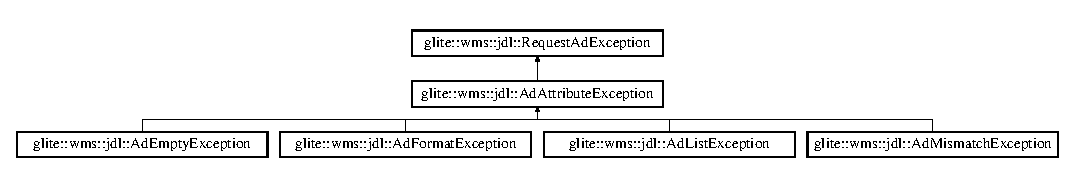
\includegraphics[height=1.89189cm]{classglite_1_1wms_1_1jdl_1_1AdAttributeException}
\end{center}
\end{figure}
\subsection*{Public Member Functions}
\begin{CompactItemize}
\item 
\hyperlink{classglite_1_1wms_1_1jdl_1_1AdAttributeException_a0}{Ad\-Attribute\-Exception::Ad\-Attribute\-Exception} (std::string file, int line, std::string method, int code, std::string exception\_\-name)
\end{CompactItemize}


\subsection{Detailed Description}
\hyperlink{classglite_1_1wms_1_1jdl_1_1AdAttributeException}{Ad\-Attribute\-Exception} - raised when a not admitted value is added/set to the attribute 



\subsection{Member Function Documentation}
\hypertarget{classglite_1_1wms_1_1jdl_1_1AdAttributeException_a0}{
\index{glite::wms::jdl::AdAttributeException@{glite::wms::jdl::Ad\-Attribute\-Exception}!AdAttributeException::AdAttributeException@{AdAttributeException::AdAttributeException}}
\index{AdAttributeException::AdAttributeException@{AdAttributeException::AdAttributeException}!glite::wms::jdl::AdAttributeException@{glite::wms::jdl::Ad\-Attribute\-Exception}}
\subsubsection[AdAttributeException::AdAttributeException]{\setlength{\rightskip}{0pt plus 5cm}glite::wms::jdl::Ad\-Attribute\-Exception::Ad\-Attribute\-Exception::Ad\-Attribute\-Exception (std::string {\em file}, int {\em line}, std::string {\em method}, int {\em code}, std::string {\em exception\_\-name})}}
\label{classglite_1_1wms_1_1jdl_1_1AdAttributeException_a0}




The documentation for this class was generated from the following file:\begin{CompactItemize}
\item 
\hyperlink{RequestAdExceptions_8h}{Request\-Ad\-Exceptions.h}\end{CompactItemize}

\hypertarget{classglite_1_1wms_1_1jdl_1_1AdClassAdException}{
\section{glite::wms::jdl::Ad\-Class\-Ad\-Exception Class Reference}
\label{classglite_1_1wms_1_1jdl_1_1AdClassAdException}\index{glite::wms::jdl::AdClassAdException@{glite::wms::jdl::AdClassAdException}}
}
{\tt \#include $<$Request\-Ad\-Exceptions.h$>$}

Inheritance diagram for glite::wms::jdl::Ad\-Class\-Ad\-Exception::\begin{figure}[H]
\begin{center}
\leavevmode
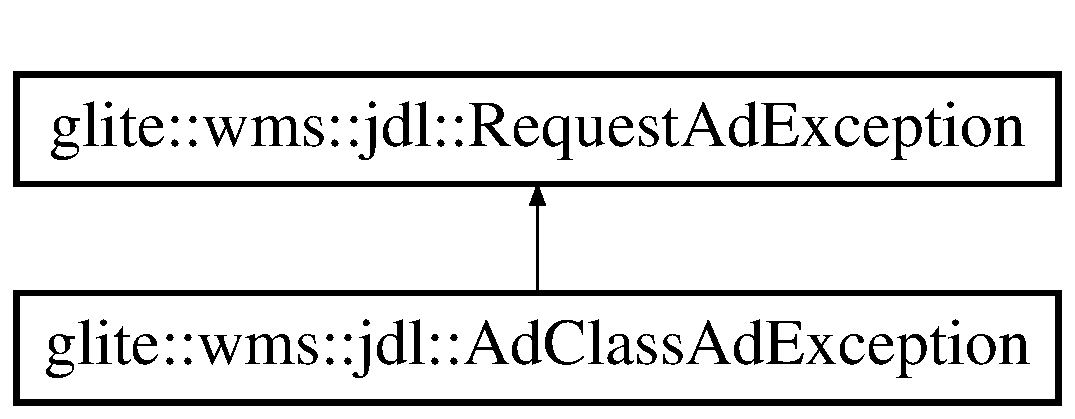
\includegraphics[height=2cm]{classglite_1_1wms_1_1jdl_1_1AdClassAdException}
\end{center}
\end{figure}
\subsection*{Public Member Functions}
\begin{CompactItemize}
\item 
\hyperlink{classglite_1_1wms_1_1jdl_1_1AdClassAdException_a0}{Ad\-Class\-Ad\-Exception::Ad\-Class\-Ad\-Exception} (std::string file, int line, std::string method, int code, std::string method\_\-name, std::string \hyperlink{classglite_1_1wms_1_1jdl_1_1RequestAdException_p0}{error\_\-description}=\char`\"{}\char`\"{})
\end{CompactItemize}


\subsection{Detailed Description}
\hyperlink{classglite_1_1wms_1_1jdl_1_1AdClassAdException}{Ad\-Class\-Ad\-Exception} - raised when Class\-Ad error is checked during add/set methods 



\subsection{Member Function Documentation}
\hypertarget{classglite_1_1wms_1_1jdl_1_1AdClassAdException_a0}{
\index{glite::wms::jdl::AdClassAdException@{glite::wms::jdl::Ad\-Class\-Ad\-Exception}!AdClassAdException::AdClassAdException@{AdClassAdException::AdClassAdException}}
\index{AdClassAdException::AdClassAdException@{AdClassAdException::AdClassAdException}!glite::wms::jdl::AdClassAdException@{glite::wms::jdl::Ad\-Class\-Ad\-Exception}}
\subsubsection[AdClassAdException::AdClassAdException]{\setlength{\rightskip}{0pt plus 5cm}glite::wms::jdl::Ad\-Class\-Ad\-Exception::Ad\-Class\-Ad\-Exception::Ad\-Class\-Ad\-Exception (std::string {\em file}, int {\em line}, std::string {\em method}, int {\em code}, std::string {\em method\_\-name}, std::string {\em error\_\-description} = \char`\"{}\char`\"{})}}
\label{classglite_1_1wms_1_1jdl_1_1AdClassAdException_a0}




The documentation for this class was generated from the following file:\begin{CompactItemize}
\item 
\hyperlink{RequestAdExceptions_8h}{Request\-Ad\-Exceptions.h}\end{CompactItemize}

\hypertarget{classglite_1_1wms_1_1jdl_1_1AdConverter}{
\section{glite::wms::jdl::Ad\-Converter Class Reference}
\label{classglite_1_1wms_1_1jdl_1_1AdConverter}\index{glite::wms::jdl::AdConverter@{glite::wms::jdl::AdConverter}}
}
utilities for converting classad expression into requestad known classes and to create Job\-Ad/Exp\-Dag\-Ad templates instances  


{\tt \#include $<$adconverter.h$>$}

\subsection*{Public Types}
\begin{CompactItemize}
\item 
enum \hyperlink{classglite_1_1wms_1_1jdl_1_1AdConverter_w9}{jobtype} \{ \par
\hyperlink{classglite_1_1wms_1_1jdl_1_1AdConverter_w9w0}{ADCONV\_\-JOBTYPE\_\-NORMAL} = 1, 
\hyperlink{classglite_1_1wms_1_1jdl_1_1AdConverter_w9w1}{ADCONV\_\-JOBTYPE\_\-PARAMETRIC} = 2, 
\hyperlink{classglite_1_1wms_1_1jdl_1_1AdConverter_w9w2}{ADCONV\_\-JOBTYPE\_\-INTERACTIVE} = 4, 
\hyperlink{classglite_1_1wms_1_1jdl_1_1AdConverter_w9w3}{ADCONV\_\-JOBTYPE\_\-MPICH} = 8, 
\par
\hyperlink{classglite_1_1wms_1_1jdl_1_1AdConverter_w9w4}{ADCONV\_\-JOBTYPE\_\-PARTITIONABLE} = 16, 
\hyperlink{classglite_1_1wms_1_1jdl_1_1AdConverter_w9w5}{ADCONV\_\-JOBTYPE\_\-CHECKPOINTABLE} = 32
 \}
\item 
enum \hyperlink{classglite_1_1wms_1_1jdl_1_1AdConverter_w10}{attribute} \{ \hyperlink{classglite_1_1wms_1_1jdl_1_1AdConverter_w10w6}{ADCONV\_\-ATTR\_\-INPUTSB} = 1, 
\hyperlink{classglite_1_1wms_1_1jdl_1_1AdConverter_w10w7}{ADCONV\_\-ATTR\_\-INPUTDATA} = 2, 
\hyperlink{classglite_1_1wms_1_1jdl_1_1AdConverter_w10w8}{ADCONV\_\-ATTR\_\-ARGUMENTS} = 4
 \}
\end{CompactItemize}
\subsection*{Static Public Member Functions}
\begin{Indent}{\bf Template creation:}\par
\begin{CompactItemize}
\item 
\hyperlink{classglite_1_1wms_1_1jdl_1_1JobAd}{Job\-Ad} $\ast$ \hyperlink{classglite_1_1wms_1_1jdl_1_1AdConverter_z21_0}{create\-Job\-Template} (int type, const std::string \&executable, const std::string \&arguments, const std::string \&requirements, const std::string \&rank, const std::string \&vo=\char`\"{}\char`\"{})
\item 
\hyperlink{classglite_1_1wms_1_1jdl_1_1JobAd}{Job\-Ad} $\ast$ \hyperlink{classglite_1_1wms_1_1jdl_1_1AdConverter_z21_1}{create\-String\-Parametric\-Template} (std::vector$<$ std::string $>$ parametrised,std::vector$<$ std::string $>$ parameters, const std::string \&requirements, const std::string \&rank, const std::string \&vo=\char`\"{}\char`\"{})
\item 
\hyperlink{classglite_1_1wms_1_1jdl_1_1JobAd}{Job\-Ad} $\ast$ \hyperlink{classglite_1_1wms_1_1jdl_1_1AdConverter_z21_2}{create\-String\-Parametric\-Template} (int parametrised,std::vector$<$ std::string $>$ parameters, const std::string \&requirements, const std::string \&rank, const std::string \&vo=\char`\"{}\char`\"{})
\item 
\hyperlink{classglite_1_1wms_1_1jdl_1_1JobAd}{Job\-Ad} $\ast$ \hyperlink{classglite_1_1wms_1_1jdl_1_1AdConverter_z21_3}{create\-Int\-Parametric\-Template} (std::vector$<$ std::string $>$ parametrised,int param\_\-number, int param\_\-start, int param\_\-step, const std::string \&requirements, const std::string \&rank, const std::string \&vo=\char`\"{}\char`\"{})
\item 
\hyperlink{classglite_1_1wms_1_1jdl_1_1JobAd}{Job\-Ad} $\ast$ \hyperlink{classglite_1_1wms_1_1jdl_1_1AdConverter_z21_4}{create\-Int\-Parametric\-Template} (int parametrised,int param\_\-number, int param\_\-start, int param\_\-step, const std::string \&requirements, const std::string \&rank, const std::string \&vo=\char`\"{}\char`\"{})
\item 
\hyperlink{classglite_1_1wms_1_1jdl_1_1ExpDagAd}{Exp\-Dag\-Ad} $\ast$ \hyperlink{classglite_1_1wms_1_1jdl_1_1AdConverter_z21_5}{create\-DAGTemplate} (\hyperlink{structglite_1_1wms_1_1jdl_1_1NodeStruct}{Node\-Struct} dependencies, const std::string \&requirements, const std::string \&rank, const std::string \&vo=\char`\"{}\char`\"{})
\item 
\hyperlink{classglite_1_1wms_1_1jdl_1_1Ad}{Ad} $\ast$ \hyperlink{classglite_1_1wms_1_1jdl_1_1AdConverter_z21_6}{create\-Collection\-Template} (unsigned int job\-Number,const std::string \&requirements, const std::string \&rank, const std::string \&vo=\char`\"{}\char`\"{})
\item 
\hyperlink{classglite_1_1wms_1_1jdl_1_1Ad}{Ad} $\ast$ \hyperlink{classglite_1_1wms_1_1jdl_1_1AdConverter_z21_7}{create\-Collection\-From\-Path} (const std::string \&path, const std::string \&vo=\char`\"{}\char`\"{})
\end{CompactItemize}
\end{Indent}
\begin{Indent}{\bf Ad conversion:}\par
\begin{CompactItemize}
\item 
\hyperlink{classglite_1_1wms_1_1jdl_1_1ExpDagAd}{Exp\-Dag\-Ad} $\ast$ \hyperlink{classglite_1_1wms_1_1jdl_1_1AdConverter_z23_0}{part2dag} (const std::string \&ad)
\item 
\hyperlink{classglite_1_1wms_1_1jdl_1_1ExpDagAd}{Exp\-Dag\-Ad} $\ast$ \hyperlink{classglite_1_1wms_1_1jdl_1_1AdConverter_z23_1}{part2dag} (\hyperlink{classglite_1_1wms_1_1jdl_1_1Ad}{Ad} $\ast$ad)
\item 
\hyperlink{classglite_1_1wms_1_1jdl_1_1ExpDagAd}{Exp\-Dag\-Ad} $\ast$ \hyperlink{classglite_1_1wms_1_1jdl_1_1AdConverter_z23_2}{collection2dag} (const std::string \&ad)
\item 
\hyperlink{classglite_1_1wms_1_1jdl_1_1ExpDagAd}{Exp\-Dag\-Ad} $\ast$ \hyperlink{classglite_1_1wms_1_1jdl_1_1AdConverter_z23_3}{collection2dag} (\hyperlink{classglite_1_1wms_1_1jdl_1_1Ad}{Ad} $\ast$ad)
\item 
\hyperlink{classglite_1_1wms_1_1jdl_1_1ExpDagAd}{Exp\-Dag\-Ad} $\ast$ \hyperlink{classglite_1_1wms_1_1jdl_1_1AdConverter_z23_4}{bulk2dag} (const std::string \&ad)
\item 
\hyperlink{classglite_1_1wms_1_1jdl_1_1ExpDagAd}{Exp\-Dag\-Ad} $\ast$ \hyperlink{classglite_1_1wms_1_1jdl_1_1AdConverter_z23_5}{bulk2dag} (\hyperlink{classglite_1_1wms_1_1jdl_1_1Ad}{Ad} $\ast$ad)
\end{CompactItemize}
\end{Indent}
\subsection*{Static Public Attributes}
\begin{CompactItemize}
\item 
const std::string \hyperlink{classglite_1_1wms_1_1jdl_1_1AdConverter_s0}{VALUES}
\item 
const std::string \hyperlink{classglite_1_1wms_1_1jdl_1_1AdConverter_s1}{VALUE}
\item 
const std::string \hyperlink{classglite_1_1wms_1_1jdl_1_1AdConverter_s2}{NODE}
\item 
const std::string \hyperlink{classglite_1_1wms_1_1jdl_1_1AdConverter_s3}{SIMPLE\_\-NODE\_\-TYPE}
\item 
const std::string \hyperlink{classglite_1_1wms_1_1jdl_1_1AdConverter_s4}{PARAMETRIC\_\-PARAMETERS}
\item 
const std::string \hyperlink{classglite_1_1wms_1_1jdl_1_1AdConverter_s5}{PARAMETRIC\_\-START}
\item 
const std::string \hyperlink{classglite_1_1wms_1_1jdl_1_1AdConverter_s6}{PARAMETRIC\_\-STEP}
\end{CompactItemize}


\subsection{Detailed Description}
utilities for converting classad expression into requestad known classes and to create Job\-Ad/Exp\-Dag\-Ad templates instances 

\hyperlink{classglite_1_1wms_1_1jdl_1_1AdConverter}{Ad\-Converter} deifines a series of utiliteis as separate static methods that allow the user to convert a Jdl into several different classad representation. it manages partitioner, collection and parametric jdls converting internally into an \hyperlink{classglite_1_1wms_1_1jdl_1_1ExpDagAd}{Exp\-Dag\-Ad} clas instance. It also provide a set of utilities to easily create valid jdl template for simple Jobs (even with jobtype different from \char`\"{}normal\char`\"{}) Dags or Collection of jobs; just by specifing a few parameters.

\begin{Desc}
\item[Version:]0.1 \end{Desc}
\begin{Desc}
\item[Date:]2004 \end{Desc}
\begin{Desc}
\item[Author:]Alessandro Maraschini $<$\href{mailto:alessandro.maraschini@datamat.it}{\tt alessandro.maraschini@datamat.it}$>$ \end{Desc}




\subsection{Member Enumeration Documentation}
\hypertarget{classglite_1_1wms_1_1jdl_1_1AdConverter_w10}{
\index{glite::wms::jdl::AdConverter@{glite::wms::jdl::Ad\-Converter}!attribute@{attribute}}
\index{attribute@{attribute}!glite::wms::jdl::AdConverter@{glite::wms::jdl::Ad\-Converter}}
\subsubsection[attribute]{\setlength{\rightskip}{0pt plus 5cm}enum \hyperlink{classglite_1_1wms_1_1jdl_1_1AdConverter_w10}{glite::wms::jdl::Ad\-Converter::attribute}}}
\label{classglite_1_1wms_1_1jdl_1_1AdConverter_w10}


Enum used to specify which attribute(s) are to be parametrised Notice: muliple attributes can be obtained by bitwise '$|$' operator. \begin{Desc}
\item[See also:]\hyperlink{classglite_1_1wms_1_1jdl_1_1AdConverter_z21_1}{create\-String\-Parametric\-Template} 

\hyperlink{classglite_1_1wms_1_1jdl_1_1AdConverter_z21_3}{create\-Int\-Parametric\-Template}\end{Desc}
\begin{Desc}
\item[Enumeration values: ]\par
\begin{description}
\index{ADCONV_ATTR_INPUTSB@{ADCONV\_\-ATTR\_\-INPUTSB}!glite::wms::jdl::AdConverter@{glite::wms::jdl::AdConverter}}\index{glite::wms::jdl::AdConverter@{glite::wms::jdl::AdConverter}!ADCONV_ATTR_INPUTSB@{ADCONV\_\-ATTR\_\-INPUTSB}}\item[{\em 
\hypertarget{classglite_1_1wms_1_1jdl_1_1AdConverter_w10w6}{
ADCONV\_\-ATTR\_\-INPUTSB}
\label{classglite_1_1wms_1_1jdl_1_1AdConverter_w10w6}
}]\index{ADCONV_ATTR_INPUTDATA@{ADCONV\_\-ATTR\_\-INPUTDATA}!glite::wms::jdl::AdConverter@{glite::wms::jdl::AdConverter}}\index{glite::wms::jdl::AdConverter@{glite::wms::jdl::AdConverter}!ADCONV_ATTR_INPUTDATA@{ADCONV\_\-ATTR\_\-INPUTDATA}}\item[{\em 
\hypertarget{classglite_1_1wms_1_1jdl_1_1AdConverter_w10w7}{
ADCONV\_\-ATTR\_\-INPUTDATA}
\label{classglite_1_1wms_1_1jdl_1_1AdConverter_w10w7}
}]\index{ADCONV_ATTR_ARGUMENTS@{ADCONV\_\-ATTR\_\-ARGUMENTS}!glite::wms::jdl::AdConverter@{glite::wms::jdl::AdConverter}}\index{glite::wms::jdl::AdConverter@{glite::wms::jdl::AdConverter}!ADCONV_ATTR_ARGUMENTS@{ADCONV\_\-ATTR\_\-ARGUMENTS}}\item[{\em 
\hypertarget{classglite_1_1wms_1_1jdl_1_1AdConverter_w10w8}{
ADCONV\_\-ATTR\_\-ARGUMENTS}
\label{classglite_1_1wms_1_1jdl_1_1AdConverter_w10w8}
}]\end{description}
\end{Desc}

\hypertarget{classglite_1_1wms_1_1jdl_1_1AdConverter_w9}{
\index{glite::wms::jdl::AdConverter@{glite::wms::jdl::Ad\-Converter}!jobtype@{jobtype}}
\index{jobtype@{jobtype}!glite::wms::jdl::AdConverter@{glite::wms::jdl::Ad\-Converter}}
\subsubsection[jobtype]{\setlength{\rightskip}{0pt plus 5cm}enum \hyperlink{classglite_1_1wms_1_1jdl_1_1AdConverter_w9}{glite::wms::jdl::Ad\-Converter::jobtype}}}
\label{classglite_1_1wms_1_1jdl_1_1AdConverter_w9}


Enum used to specify the Jobtype of a job Notice: muliple job type can be obtained by bitwise '$|$' operator. \begin{Desc}
\item[See also:]\hyperlink{classglite_1_1wms_1_1jdl_1_1AdConverter_z21_0}{create\-Job\-Template} \end{Desc}
\begin{Desc}
\item[Enumeration values: ]\par
\begin{description}
\index{ADCONV_JOBTYPE_NORMAL@{ADCONV\_\-JOBTYPE\_\-NORMAL}!glite::wms::jdl::AdConverter@{glite::wms::jdl::AdConverter}}\index{glite::wms::jdl::AdConverter@{glite::wms::jdl::AdConverter}!ADCONV_JOBTYPE_NORMAL@{ADCONV\_\-JOBTYPE\_\-NORMAL}}\item[{\em 
\hypertarget{classglite_1_1wms_1_1jdl_1_1AdConverter_w9w0}{
ADCONV\_\-JOBTYPE\_\-NORMAL}
\label{classglite_1_1wms_1_1jdl_1_1AdConverter_w9w0}
}]\index{ADCONV_JOBTYPE_PARAMETRIC@{ADCONV\_\-JOBTYPE\_\-PARAMETRIC}!glite::wms::jdl::AdConverter@{glite::wms::jdl::AdConverter}}\index{glite::wms::jdl::AdConverter@{glite::wms::jdl::AdConverter}!ADCONV_JOBTYPE_PARAMETRIC@{ADCONV\_\-JOBTYPE\_\-PARAMETRIC}}\item[{\em 
\hypertarget{classglite_1_1wms_1_1jdl_1_1AdConverter_w9w1}{
ADCONV\_\-JOBTYPE\_\-PARAMETRIC}
\label{classglite_1_1wms_1_1jdl_1_1AdConverter_w9w1}
}]\index{ADCONV_JOBTYPE_INTERACTIVE@{ADCONV\_\-JOBTYPE\_\-INTERACTIVE}!glite::wms::jdl::AdConverter@{glite::wms::jdl::AdConverter}}\index{glite::wms::jdl::AdConverter@{glite::wms::jdl::AdConverter}!ADCONV_JOBTYPE_INTERACTIVE@{ADCONV\_\-JOBTYPE\_\-INTERACTIVE}}\item[{\em 
\hypertarget{classglite_1_1wms_1_1jdl_1_1AdConverter_w9w2}{
ADCONV\_\-JOBTYPE\_\-INTERACTIVE}
\label{classglite_1_1wms_1_1jdl_1_1AdConverter_w9w2}
}]\index{ADCONV_JOBTYPE_MPICH@{ADCONV\_\-JOBTYPE\_\-MPICH}!glite::wms::jdl::AdConverter@{glite::wms::jdl::AdConverter}}\index{glite::wms::jdl::AdConverter@{glite::wms::jdl::AdConverter}!ADCONV_JOBTYPE_MPICH@{ADCONV\_\-JOBTYPE\_\-MPICH}}\item[{\em 
\hypertarget{classglite_1_1wms_1_1jdl_1_1AdConverter_w9w3}{
ADCONV\_\-JOBTYPE\_\-MPICH}
\label{classglite_1_1wms_1_1jdl_1_1AdConverter_w9w3}
}]\index{ADCONV_JOBTYPE_PARTITIONABLE@{ADCONV\_\-JOBTYPE\_\-PARTITIONABLE}!glite::wms::jdl::AdConverter@{glite::wms::jdl::AdConverter}}\index{glite::wms::jdl::AdConverter@{glite::wms::jdl::AdConverter}!ADCONV_JOBTYPE_PARTITIONABLE@{ADCONV\_\-JOBTYPE\_\-PARTITIONABLE}}\item[{\em 
\hypertarget{classglite_1_1wms_1_1jdl_1_1AdConverter_w9w4}{
ADCONV\_\-JOBTYPE\_\-PARTITIONABLE}
\label{classglite_1_1wms_1_1jdl_1_1AdConverter_w9w4}
}]\index{ADCONV_JOBTYPE_CHECKPOINTABLE@{ADCONV\_\-JOBTYPE\_\-CHECKPOINTABLE}!glite::wms::jdl::AdConverter@{glite::wms::jdl::AdConverter}}\index{glite::wms::jdl::AdConverter@{glite::wms::jdl::AdConverter}!ADCONV_JOBTYPE_CHECKPOINTABLE@{ADCONV\_\-JOBTYPE\_\-CHECKPOINTABLE}}\item[{\em 
\hypertarget{classglite_1_1wms_1_1jdl_1_1AdConverter_w9w5}{
ADCONV\_\-JOBTYPE\_\-CHECKPOINTABLE}
\label{classglite_1_1wms_1_1jdl_1_1AdConverter_w9w5}
}]\end{description}
\end{Desc}



\subsection{Member Function Documentation}
\hypertarget{classglite_1_1wms_1_1jdl_1_1AdConverter_z23_5}{
\index{glite::wms::jdl::AdConverter@{glite::wms::jdl::Ad\-Converter}!bulk2dag@{bulk2dag}}
\index{bulk2dag@{bulk2dag}!glite::wms::jdl::AdConverter@{glite::wms::jdl::Ad\-Converter}}
\subsubsection[bulk2dag]{\setlength{\rightskip}{0pt plus 5cm}\hyperlink{classglite_1_1wms_1_1jdl_1_1ExpDagAd}{Exp\-Dag\-Ad}$\ast$ glite::wms::jdl::Ad\-Converter::bulk2dag (\hyperlink{classglite_1_1wms_1_1jdl_1_1Ad}{Ad} $\ast$ {\em ad})\hspace{0.3cm}{\tt  \mbox{[}static\mbox{]}}}}
\label{classglite_1_1wms_1_1jdl_1_1AdConverter_z23_5}


utility that converts the jdl of a parametric job into a Dag\-Ad \begin{Desc}
\item[Parameters:]
\begin{description}
\item[{\em ad}]the Class\-Ad representing the JDL of a parametric job \end{description}
\end{Desc}
\begin{Desc}
\item[Returns:]the converted \hyperlink{classglite_1_1wms_1_1jdl_1_1ExpDagAd}{Exp\-Dag\-Ad} instance\end{Desc}
\hypertarget{classglite_1_1wms_1_1jdl_1_1AdConverter_z23_4}{
\index{glite::wms::jdl::AdConverter@{glite::wms::jdl::Ad\-Converter}!bulk2dag@{bulk2dag}}
\index{bulk2dag@{bulk2dag}!glite::wms::jdl::AdConverter@{glite::wms::jdl::Ad\-Converter}}
\subsubsection[bulk2dag]{\setlength{\rightskip}{0pt plus 5cm}\hyperlink{classglite_1_1wms_1_1jdl_1_1ExpDagAd}{Exp\-Dag\-Ad}$\ast$ glite::wms::jdl::Ad\-Converter::bulk2dag (const std::string \& {\em ad})\hspace{0.3cm}{\tt  \mbox{[}static\mbox{]}}}}
\label{classglite_1_1wms_1_1jdl_1_1AdConverter_z23_4}


utility that converts the jdl of a parametric job into a Dag\-Ad \begin{Desc}
\item[Parameters:]
\begin{description}
\item[{\em jdl}]string representing the classad of a parametric job \end{description}
\end{Desc}
\begin{Desc}
\item[Returns:]the converted \hyperlink{classglite_1_1wms_1_1jdl_1_1ExpDagAd}{Exp\-Dag\-Ad} instance\end{Desc}
\hypertarget{classglite_1_1wms_1_1jdl_1_1AdConverter_z23_3}{
\index{glite::wms::jdl::AdConverter@{glite::wms::jdl::Ad\-Converter}!collection2dag@{collection2dag}}
\index{collection2dag@{collection2dag}!glite::wms::jdl::AdConverter@{glite::wms::jdl::Ad\-Converter}}
\subsubsection[collection2dag]{\setlength{\rightskip}{0pt plus 5cm}\hyperlink{classglite_1_1wms_1_1jdl_1_1ExpDagAd}{Exp\-Dag\-Ad}$\ast$ glite::wms::jdl::Ad\-Converter::collection2dag (\hyperlink{classglite_1_1wms_1_1jdl_1_1Ad}{Ad} $\ast$ {\em ad})\hspace{0.3cm}{\tt  \mbox{[}static\mbox{]}}}}
\label{classglite_1_1wms_1_1jdl_1_1AdConverter_z23_3}


utility that converts the jdl of a collection into a Dag\-Ad \begin{Desc}
\item[Parameters:]
\begin{description}
\item[{\em ad}]the Class\-Ad representing the JDL of a collection of jobs \end{description}
\end{Desc}
\begin{Desc}
\item[Returns:]the converted \hyperlink{classglite_1_1wms_1_1jdl_1_1ExpDagAd}{Exp\-Dag\-Ad} instance\end{Desc}
\hypertarget{classglite_1_1wms_1_1jdl_1_1AdConverter_z23_2}{
\index{glite::wms::jdl::AdConverter@{glite::wms::jdl::Ad\-Converter}!collection2dag@{collection2dag}}
\index{collection2dag@{collection2dag}!glite::wms::jdl::AdConverter@{glite::wms::jdl::Ad\-Converter}}
\subsubsection[collection2dag]{\setlength{\rightskip}{0pt plus 5cm}\hyperlink{classglite_1_1wms_1_1jdl_1_1ExpDagAd}{Exp\-Dag\-Ad}$\ast$ glite::wms::jdl::Ad\-Converter::collection2dag (const std::string \& {\em ad})\hspace{0.3cm}{\tt  \mbox{[}static\mbox{]}}}}
\label{classglite_1_1wms_1_1jdl_1_1AdConverter_z23_2}


utility that converts the jdl of a collection into a Dag\-Ad \begin{Desc}
\item[Parameters:]
\begin{description}
\item[{\em jdl}]string representing the classad of a collection of jobs \end{description}
\end{Desc}
\begin{Desc}
\item[Returns:]the converted \hyperlink{classglite_1_1wms_1_1jdl_1_1ExpDagAd}{Exp\-Dag\-Ad} instance\end{Desc}
\hypertarget{classglite_1_1wms_1_1jdl_1_1AdConverter_z21_7}{
\index{glite::wms::jdl::AdConverter@{glite::wms::jdl::Ad\-Converter}!createCollectionFromPath@{createCollectionFromPath}}
\index{createCollectionFromPath@{createCollectionFromPath}!glite::wms::jdl::AdConverter@{glite::wms::jdl::Ad\-Converter}}
\subsubsection[createCollectionFromPath]{\setlength{\rightskip}{0pt plus 5cm}\hyperlink{classglite_1_1wms_1_1jdl_1_1Ad}{Ad}$\ast$ glite::wms::jdl::Ad\-Converter::create\-Collection\-From\-Path (const std::string \& {\em path}, const std::string \& {\em vo} = \char`\"{}\char`\"{})\hspace{0.3cm}{\tt  \mbox{[}static\mbox{]}}}}
\label{classglite_1_1wms_1_1jdl_1_1AdConverter_z21_7}


Load all the JDL files stored in a specified path and put them all inside a collection of jobs \begin{Desc}
\item[Parameters:]
\begin{description}
\item[{\em path}]the directory where to look for JDL files to be added to the collection \item[{\em vo}]the Virtual\-Organisation name to be used by all the jobs in the collection \end{description}
\end{Desc}
\begin{Desc}
\item[Returns:]the Class\-Ad template istance\end{Desc}
\hypertarget{classglite_1_1wms_1_1jdl_1_1AdConverter_z21_6}{
\index{glite::wms::jdl::AdConverter@{glite::wms::jdl::Ad\-Converter}!createCollectionTemplate@{createCollectionTemplate}}
\index{createCollectionTemplate@{createCollectionTemplate}!glite::wms::jdl::AdConverter@{glite::wms::jdl::Ad\-Converter}}
\subsubsection[createCollectionTemplate]{\setlength{\rightskip}{0pt plus 5cm}\hyperlink{classglite_1_1wms_1_1jdl_1_1Ad}{Ad}$\ast$ glite::wms::jdl::Ad\-Converter::create\-Collection\-Template (unsigned int {\em job\-Number}, const std::string \& {\em requirements}, const std::string \& {\em rank}, const std::string \& {\em vo} = \char`\"{}\char`\"{})\hspace{0.3cm}{\tt  \mbox{[}static\mbox{]}}}}
\label{classglite_1_1wms_1_1jdl_1_1AdConverter_z21_6}


Create a valid template JDL for a Collection of jobs \begin{Desc}
\item[Parameters:]
\begin{description}
\item[{\em job\-Number}]the number of jobs to be created for the collection \item[{\em requirements}]a string representing the expression describing the requirements (which is an attribute of boolean type) for all the jobs in the collection \item[{\em rank}]a string representing the expression for the rank (which is an attribute of double type) for all the jobs in the collection \item[{\em vo}]the Virtual\-Organisation name to be used by all the jobs in the collection \end{description}
\end{Desc}
\begin{Desc}
\item[Returns:]the Class\-Ad template istance\end{Desc}
\hypertarget{classglite_1_1wms_1_1jdl_1_1AdConverter_z21_5}{
\index{glite::wms::jdl::AdConverter@{glite::wms::jdl::Ad\-Converter}!createDAGTemplate@{createDAGTemplate}}
\index{createDAGTemplate@{createDAGTemplate}!glite::wms::jdl::AdConverter@{glite::wms::jdl::Ad\-Converter}}
\subsubsection[createDAGTemplate]{\setlength{\rightskip}{0pt plus 5cm}\hyperlink{classglite_1_1wms_1_1jdl_1_1ExpDagAd}{Exp\-Dag\-Ad}$\ast$ glite::wms::jdl::Ad\-Converter::create\-DAGTemplate (\hyperlink{structglite_1_1wms_1_1jdl_1_1NodeStruct}{Node\-Struct} {\em dependencies}, const std::string \& {\em requirements}, const std::string \& {\em rank}, const std::string \& {\em vo} = \char`\"{}\char`\"{})\hspace{0.3cm}{\tt  \mbox{[}static\mbox{]}}}}
\label{classglite_1_1wms_1_1jdl_1_1AdConverter_z21_5}


Create a valid template JDL for a Dag \begin{Desc}
\item[Parameters:]
\begin{description}
\item[{\em dependencies}]the dependency structure of the dag: each node must list all the nodes that depends on it. \item[{\em requirements}]a string representing the expression describing the requirements (which is an attribute of boolean type) for all the nodes of the dag \item[{\em rank}]a string representing the expression for the rank (which is an attribute of double type) for all the nodes of the dag \item[{\em vo}]the Virtual\-Organisation name to be used for all the nodes of the dag \end{description}
\end{Desc}
\begin{Desc}
\item[Returns:]the \hyperlink{classglite_1_1wms_1_1jdl_1_1ExpDagAd}{Exp\-Dag\-Ad} template istance\end{Desc}
\hypertarget{classglite_1_1wms_1_1jdl_1_1AdConverter_z21_4}{
\index{glite::wms::jdl::AdConverter@{glite::wms::jdl::Ad\-Converter}!createIntParametricTemplate@{createIntParametricTemplate}}
\index{createIntParametricTemplate@{createIntParametricTemplate}!glite::wms::jdl::AdConverter@{glite::wms::jdl::Ad\-Converter}}
\subsubsection[createIntParametricTemplate]{\setlength{\rightskip}{0pt plus 5cm}\hyperlink{classglite_1_1wms_1_1jdl_1_1JobAd}{Job\-Ad}$\ast$ glite::wms::jdl::Ad\-Converter::create\-Int\-Parametric\-Template (int {\em parametrised}, int {\em param\_\-number}, int {\em param\_\-start}, int {\em param\_\-step}, const std::string \& {\em requirements}, const std::string \& {\em rank}, const std::string \& {\em vo} = \char`\"{}\char`\"{})\hspace{0.3cm}{\tt  \mbox{[}static\mbox{]}}}}
\label{classglite_1_1wms_1_1jdl_1_1AdConverter_z21_4}


\hypertarget{classglite_1_1wms_1_1jdl_1_1AdConverter_z21_3}{
\index{glite::wms::jdl::AdConverter@{glite::wms::jdl::Ad\-Converter}!createIntParametricTemplate@{createIntParametricTemplate}}
\index{createIntParametricTemplate@{createIntParametricTemplate}!glite::wms::jdl::AdConverter@{glite::wms::jdl::Ad\-Converter}}
\subsubsection[createIntParametricTemplate]{\setlength{\rightskip}{0pt plus 5cm}\hyperlink{classglite_1_1wms_1_1jdl_1_1JobAd}{Job\-Ad}$\ast$ glite::wms::jdl::Ad\-Converter::create\-Int\-Parametric\-Template (std::vector$<$ std::string $>$ {\em parametrised}, int {\em param\_\-number}, int {\em param\_\-start}, int {\em param\_\-step}, const std::string \& {\em requirements}, const std::string \& {\em rank}, const std::string \& {\em vo} = \char`\"{}\char`\"{})\hspace{0.3cm}{\tt  \mbox{[}static\mbox{]}}}}
\label{classglite_1_1wms_1_1jdl_1_1AdConverter_z21_3}


Create a valid Parametric \begin{Desc}
\item[Parameters:]
\begin{description}
\item[{\em parametrised}]all the attributes that contains reference to a parameter. Multiple attributes can be specified toghegher through the bitwise '$|$' operator ( as specified in \hyperlink{classglite_1_1wms_1_1jdl_1_1AdConverter_w10}{attribute}) \item[{\em param\_\-number}]the number of different parameters to be created \item[{\em param\_\-start}](default value is 0) the starting point where to begin to parametrise \item[{\em param\_\-step}](default value is 1) the step between one parameter and the next one among param\_\-start \item[{\em requirements}]a string representing the expression describing all the Job requirements (which is an attribute of boolean type) \item[{\em rank}]a string representing the expression for the rank (which is an attribute of double type) of the resource \item[{\em vo}]the Virtual\-Organisation name to be used \end{description}
\end{Desc}
\begin{Desc}
\item[Returns:]the \hyperlink{classglite_1_1wms_1_1jdl_1_1JobAd}{Job\-Ad} of a parametric job \end{Desc}
\hypertarget{classglite_1_1wms_1_1jdl_1_1AdConverter_z21_0}{
\index{glite::wms::jdl::AdConverter@{glite::wms::jdl::Ad\-Converter}!createJobTemplate@{createJobTemplate}}
\index{createJobTemplate@{createJobTemplate}!glite::wms::jdl::AdConverter@{glite::wms::jdl::Ad\-Converter}}
\subsubsection[createJobTemplate]{\setlength{\rightskip}{0pt plus 5cm}\hyperlink{classglite_1_1wms_1_1jdl_1_1JobAd}{Job\-Ad}$\ast$ glite::wms::jdl::Ad\-Converter::create\-Job\-Template (int {\em type}, const std::string \& {\em executable}, const std::string \& {\em arguments}, const std::string \& {\em requirements}, const std::string \& {\em rank}, const std::string \& {\em vo} = \char`\"{}\char`\"{})\hspace{0.3cm}{\tt  \mbox{[}static\mbox{]}}}}
\label{classglite_1_1wms_1_1jdl_1_1AdConverter_z21_0}


Create a valid JDL ready for submission. \begin{Desc}
\item[Parameters:]
\begin{description}
\item[{\em type}]the jobtype of the job. Multiple jobtype can be specified toghether through the bitwise '$|$' operator ( as specified in \hyperlink{classglite_1_1wms_1_1jdl_1_1AdConverter_w9}{jobtype}) \item[{\em executable}]the simple file name to be executed (if local) or the full path if stored in the remote machine. In the former case the full path of the file must be specified in the inputsandbox attribute \item[{\em arguments}]a string representing the arguments (if needed) of the executable file (empty \char`\"{}\char`\"{} string if not needed) \item[{\em requirements}]a string representing the expression describing all the Job requirements (which is an attribute of boolean type) \item[{\em rank}]a string representing the expression for the rank (which is an attribute of double type) of the resource \item[{\em vo}]the Virtual\-Organisation name to be used \end{description}
\end{Desc}
\begin{Desc}
\item[Returns:]the \hyperlink{classglite_1_1wms_1_1jdl_1_1JobAd}{Job\-Ad} template instance\end{Desc}
\hypertarget{classglite_1_1wms_1_1jdl_1_1AdConverter_z21_2}{
\index{glite::wms::jdl::AdConverter@{glite::wms::jdl::Ad\-Converter}!createStringParametricTemplate@{createStringParametricTemplate}}
\index{createStringParametricTemplate@{createStringParametricTemplate}!glite::wms::jdl::AdConverter@{glite::wms::jdl::Ad\-Converter}}
\subsubsection[createStringParametricTemplate]{\setlength{\rightskip}{0pt plus 5cm}\hyperlink{classglite_1_1wms_1_1jdl_1_1JobAd}{Job\-Ad}$\ast$ glite::wms::jdl::Ad\-Converter::create\-String\-Parametric\-Template (int {\em parametrised}, std::vector$<$ std::string $>$ {\em parameters}, const std::string \& {\em requirements}, const std::string \& {\em rank}, const std::string \& {\em vo} = \char`\"{}\char`\"{})\hspace{0.3cm}{\tt  \mbox{[}static\mbox{]}}}}
\label{classglite_1_1wms_1_1jdl_1_1AdConverter_z21_2}


\hypertarget{classglite_1_1wms_1_1jdl_1_1AdConverter_z21_1}{
\index{glite::wms::jdl::AdConverter@{glite::wms::jdl::Ad\-Converter}!createStringParametricTemplate@{createStringParametricTemplate}}
\index{createStringParametricTemplate@{createStringParametricTemplate}!glite::wms::jdl::AdConverter@{glite::wms::jdl::Ad\-Converter}}
\subsubsection[createStringParametricTemplate]{\setlength{\rightskip}{0pt plus 5cm}\hyperlink{classglite_1_1wms_1_1jdl_1_1JobAd}{Job\-Ad}$\ast$ glite::wms::jdl::Ad\-Converter::create\-String\-Parametric\-Template (std::vector$<$ std::string $>$ {\em parametrised}, std::vector$<$ std::string $>$ {\em parameters}, const std::string \& {\em requirements}, const std::string \& {\em rank}, const std::string \& {\em vo} = \char`\"{}\char`\"{})\hspace{0.3cm}{\tt  \mbox{[}static\mbox{]}}}}
\label{classglite_1_1wms_1_1jdl_1_1AdConverter_z21_1}


Create a valid Parametric \begin{Desc}
\item[Parameters:]
\begin{description}
\item[{\em parametrised}]all the attributes that contains reference to a parameter. Multiple attributes can be specified toghegher through the bitwise '$|$' operator ( as specified in \hyperlink{classglite_1_1wms_1_1jdl_1_1AdConverter_w10}{attribute}) \item[{\em parameters}]a vector containing all the parameters \item[{\em requirements}]a string representing the expression describing all the Job requirements (which is an attribute of boolean type) \item[{\em rank}]a string representing the expression for the rank (which is an attribute of double type) of the resource \item[{\em vo}]the Virtual\-Organisation name to be used \end{description}
\end{Desc}
\begin{Desc}
\item[Returns:]the \hyperlink{classglite_1_1wms_1_1jdl_1_1JobAd}{Job\-Ad} of a parametric job\end{Desc}
\hypertarget{classglite_1_1wms_1_1jdl_1_1AdConverter_z23_1}{
\index{glite::wms::jdl::AdConverter@{glite::wms::jdl::Ad\-Converter}!part2dag@{part2dag}}
\index{part2dag@{part2dag}!glite::wms::jdl::AdConverter@{glite::wms::jdl::Ad\-Converter}}
\subsubsection[part2dag]{\setlength{\rightskip}{0pt plus 5cm}\hyperlink{classglite_1_1wms_1_1jdl_1_1ExpDagAd}{Exp\-Dag\-Ad}$\ast$ glite::wms::jdl::Ad\-Converter::part2dag (\hyperlink{classglite_1_1wms_1_1jdl_1_1Ad}{Ad} $\ast$ {\em ad})\hspace{0.3cm}{\tt  \mbox{[}static\mbox{]}}}}
\label{classglite_1_1wms_1_1jdl_1_1AdConverter_z23_1}


utility that converts the jdl of a partitioner job into a Dag\-Ad \begin{Desc}
\item[Parameters:]
\begin{description}
\item[{\em ad}]the Class\-Ad representing the JDL of a partitioner job \end{description}
\end{Desc}
\begin{Desc}
\item[Returns:]the converted \hyperlink{classglite_1_1wms_1_1jdl_1_1ExpDagAd}{Exp\-Dag\-Ad} instance\end{Desc}
\hypertarget{classglite_1_1wms_1_1jdl_1_1AdConverter_z23_0}{
\index{glite::wms::jdl::AdConverter@{glite::wms::jdl::Ad\-Converter}!part2dag@{part2dag}}
\index{part2dag@{part2dag}!glite::wms::jdl::AdConverter@{glite::wms::jdl::Ad\-Converter}}
\subsubsection[part2dag]{\setlength{\rightskip}{0pt plus 5cm}\hyperlink{classglite_1_1wms_1_1jdl_1_1ExpDagAd}{Exp\-Dag\-Ad}$\ast$ glite::wms::jdl::Ad\-Converter::part2dag (const std::string \& {\em ad})\hspace{0.3cm}{\tt  \mbox{[}static\mbox{]}}}}
\label{classglite_1_1wms_1_1jdl_1_1AdConverter_z23_0}


utility that converts the jdl of a partitioner job into a Dag\-Ad \begin{Desc}
\item[Parameters:]
\begin{description}
\item[{\em jdl}]string representing the classad of a partitioner job \end{description}
\end{Desc}
\begin{Desc}
\item[Returns:]the converted \hyperlink{classglite_1_1wms_1_1jdl_1_1ExpDagAd}{Exp\-Dag\-Ad} instance\end{Desc}


\subsection{Member Data Documentation}
\hypertarget{classglite_1_1wms_1_1jdl_1_1AdConverter_s2}{
\index{glite::wms::jdl::AdConverter@{glite::wms::jdl::Ad\-Converter}!NODE@{NODE}}
\index{NODE@{NODE}!glite::wms::jdl::AdConverter@{glite::wms::jdl::Ad\-Converter}}
\subsubsection[NODE]{\setlength{\rightskip}{0pt plus 5cm}const std::string \hyperlink{classglite_1_1wms_1_1jdl_1_1AdConverter_s2}{glite::wms::jdl::Ad\-Converter::NODE}\hspace{0.3cm}{\tt  \mbox{[}static\mbox{]}}}}
\label{classglite_1_1wms_1_1jdl_1_1AdConverter_s2}


\hypertarget{classglite_1_1wms_1_1jdl_1_1AdConverter_s4}{
\index{glite::wms::jdl::AdConverter@{glite::wms::jdl::Ad\-Converter}!PARAMETRIC_PARAMETERS@{PARAMETRIC\_\-PARAMETERS}}
\index{PARAMETRIC_PARAMETERS@{PARAMETRIC\_\-PARAMETERS}!glite::wms::jdl::AdConverter@{glite::wms::jdl::Ad\-Converter}}
\subsubsection[PARAMETRIC\_\-PARAMETERS]{\setlength{\rightskip}{0pt plus 5cm}const std::string \hyperlink{classglite_1_1wms_1_1jdl_1_1AdConverter_s4}{glite::wms::jdl::Ad\-Converter::PARAMETRIC\_\-PARAMETERS}\hspace{0.3cm}{\tt  \mbox{[}static\mbox{]}}}}
\label{classglite_1_1wms_1_1jdl_1_1AdConverter_s4}


\hypertarget{classglite_1_1wms_1_1jdl_1_1AdConverter_s5}{
\index{glite::wms::jdl::AdConverter@{glite::wms::jdl::Ad\-Converter}!PARAMETRIC_START@{PARAMETRIC\_\-START}}
\index{PARAMETRIC_START@{PARAMETRIC\_\-START}!glite::wms::jdl::AdConverter@{glite::wms::jdl::Ad\-Converter}}
\subsubsection[PARAMETRIC\_\-START]{\setlength{\rightskip}{0pt plus 5cm}const std::string \hyperlink{classglite_1_1wms_1_1jdl_1_1AdConverter_s5}{glite::wms::jdl::Ad\-Converter::PARAMETRIC\_\-START}\hspace{0.3cm}{\tt  \mbox{[}static\mbox{]}}}}
\label{classglite_1_1wms_1_1jdl_1_1AdConverter_s5}


\hypertarget{classglite_1_1wms_1_1jdl_1_1AdConverter_s6}{
\index{glite::wms::jdl::AdConverter@{glite::wms::jdl::Ad\-Converter}!PARAMETRIC_STEP@{PARAMETRIC\_\-STEP}}
\index{PARAMETRIC_STEP@{PARAMETRIC\_\-STEP}!glite::wms::jdl::AdConverter@{glite::wms::jdl::Ad\-Converter}}
\subsubsection[PARAMETRIC\_\-STEP]{\setlength{\rightskip}{0pt plus 5cm}const std::string \hyperlink{classglite_1_1wms_1_1jdl_1_1AdConverter_s6}{glite::wms::jdl::Ad\-Converter::PARAMETRIC\_\-STEP}\hspace{0.3cm}{\tt  \mbox{[}static\mbox{]}}}}
\label{classglite_1_1wms_1_1jdl_1_1AdConverter_s6}


\hypertarget{classglite_1_1wms_1_1jdl_1_1AdConverter_s3}{
\index{glite::wms::jdl::AdConverter@{glite::wms::jdl::Ad\-Converter}!SIMPLE_NODE_TYPE@{SIMPLE\_\-NODE\_\-TYPE}}
\index{SIMPLE_NODE_TYPE@{SIMPLE\_\-NODE\_\-TYPE}!glite::wms::jdl::AdConverter@{glite::wms::jdl::Ad\-Converter}}
\subsubsection[SIMPLE\_\-NODE\_\-TYPE]{\setlength{\rightskip}{0pt plus 5cm}const std::string \hyperlink{classglite_1_1wms_1_1jdl_1_1AdConverter_s3}{glite::wms::jdl::Ad\-Converter::SIMPLE\_\-NODE\_\-TYPE}\hspace{0.3cm}{\tt  \mbox{[}static\mbox{]}}}}
\label{classglite_1_1wms_1_1jdl_1_1AdConverter_s3}


\hypertarget{classglite_1_1wms_1_1jdl_1_1AdConverter_s1}{
\index{glite::wms::jdl::AdConverter@{glite::wms::jdl::Ad\-Converter}!VALUE@{VALUE}}
\index{VALUE@{VALUE}!glite::wms::jdl::AdConverter@{glite::wms::jdl::Ad\-Converter}}
\subsubsection[VALUE]{\setlength{\rightskip}{0pt plus 5cm}const std::string \hyperlink{classglite_1_1wms_1_1jdl_1_1AdConverter_s1}{glite::wms::jdl::Ad\-Converter::VALUE}\hspace{0.3cm}{\tt  \mbox{[}static\mbox{]}}}}
\label{classglite_1_1wms_1_1jdl_1_1AdConverter_s1}


\hypertarget{classglite_1_1wms_1_1jdl_1_1AdConverter_s0}{
\index{glite::wms::jdl::AdConverter@{glite::wms::jdl::Ad\-Converter}!VALUES@{VALUES}}
\index{VALUES@{VALUES}!glite::wms::jdl::AdConverter@{glite::wms::jdl::Ad\-Converter}}
\subsubsection[VALUES]{\setlength{\rightskip}{0pt plus 5cm}const std::string \hyperlink{classglite_1_1wms_1_1jdl_1_1AdConverter_s0}{glite::wms::jdl::Ad\-Converter::VALUES}\hspace{0.3cm}{\tt  \mbox{[}static\mbox{]}}}}
\label{classglite_1_1wms_1_1jdl_1_1AdConverter_s0}




The documentation for this class was generated from the following file:\begin{CompactItemize}
\item 
\hyperlink{adconverter_8h}{adconverter.h}\end{CompactItemize}

\hypertarget{classglite_1_1wms_1_1jdl_1_1AdEmptyException}{
\section{glite::wms::jdl::Ad\-Empty\-Exception Class Reference}
\label{classglite_1_1wms_1_1jdl_1_1AdEmptyException}\index{glite::wms::jdl::AdEmptyException@{glite::wms::jdl::AdEmptyException}}
}
{\tt \#include $<$Request\-Ad\-Exceptions.h$>$}

Inheritance diagram for glite::wms::jdl::Ad\-Empty\-Exception::\begin{figure}[H]
\begin{center}
\leavevmode
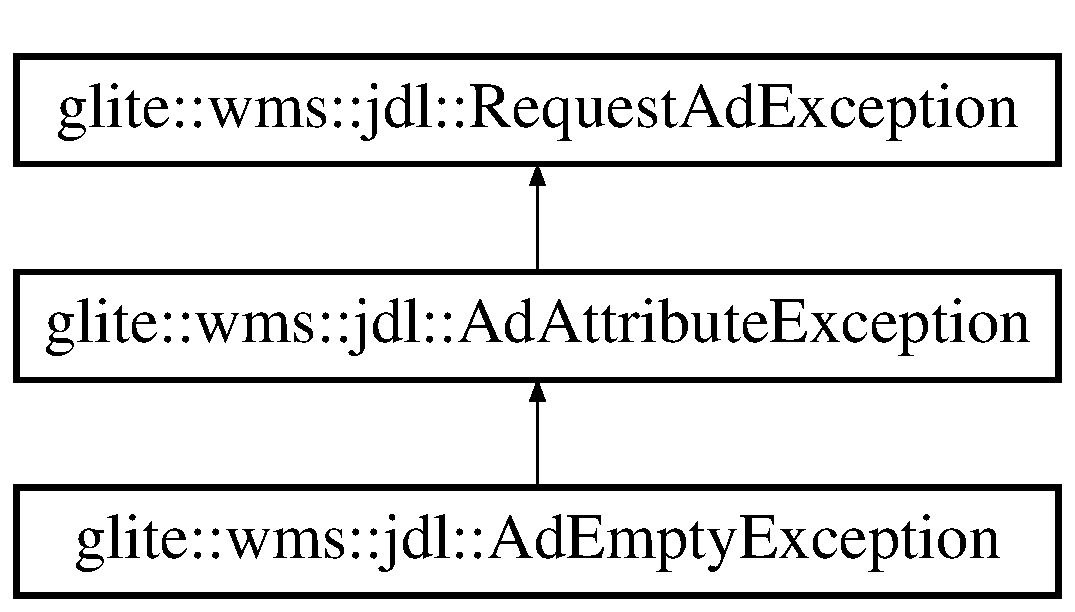
\includegraphics[height=3cm]{classglite_1_1wms_1_1jdl_1_1AdEmptyException}
\end{center}
\end{figure}
\subsection*{Public Member Functions}
\begin{CompactItemize}
\item 
\hyperlink{classglite_1_1wms_1_1jdl_1_1AdEmptyException_a0}{Ad\-Empty\-Exception} (std::string file, int line, std::string method, int code, std::string attr\_\-name)
\end{CompactItemize}


\subsection{Detailed Description}
\hyperlink{classglite_1_1wms_1_1jdl_1_1AdEmptyException}{Ad\-Empty\-Exception} - raised when an set method is made on a empty attribute 



\subsection{Constructor \& Destructor Documentation}
\hypertarget{classglite_1_1wms_1_1jdl_1_1AdEmptyException_a0}{
\index{glite::wms::jdl::AdEmptyException@{glite::wms::jdl::Ad\-Empty\-Exception}!AdEmptyException@{AdEmptyException}}
\index{AdEmptyException@{AdEmptyException}!glite::wms::jdl::AdEmptyException@{glite::wms::jdl::Ad\-Empty\-Exception}}
\subsubsection[AdEmptyException]{\setlength{\rightskip}{0pt plus 5cm}glite::wms::jdl::Ad\-Empty\-Exception::Ad\-Empty\-Exception (std::string {\em file}, int {\em line}, std::string {\em method}, int {\em code}, std::string {\em attr\_\-name})}}
\label{classglite_1_1wms_1_1jdl_1_1AdEmptyException_a0}


\hyperlink{classglite_1_1wms_1_1jdl_1_1AdEmptyException}{Ad\-Empty\-Exception} Constructor 

The documentation for this class was generated from the following file:\begin{CompactItemize}
\item 
\hyperlink{RequestAdExceptions_8h}{Request\-Ad\-Exceptions.h}\end{CompactItemize}

\hypertarget{classglite_1_1wms_1_1jdl_1_1AdFormatException}{
\section{glite::wms::jdl::Ad\-Format\-Exception Class Reference}
\label{classglite_1_1wms_1_1jdl_1_1AdFormatException}\index{glite::wms::jdl::AdFormatException@{glite::wms::jdl::AdFormatException}}
}
{\tt \#include $<$Request\-Ad\-Exceptions.h$>$}

Inheritance diagram for glite::wms::jdl::Ad\-Format\-Exception::\begin{figure}[H]
\begin{center}
\leavevmode
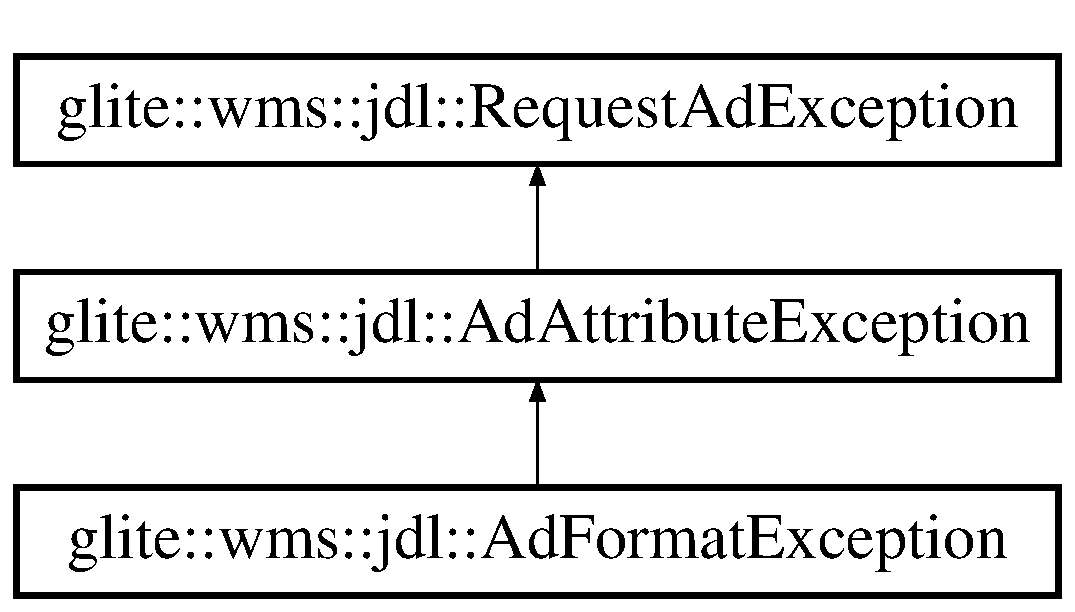
\includegraphics[height=3cm]{classglite_1_1wms_1_1jdl_1_1AdFormatException}
\end{center}
\end{figure}
\subsection*{Public Member Functions}
\begin{CompactItemize}
\item 
\hyperlink{classglite_1_1wms_1_1jdl_1_1AdFormatException_a0}{Ad\-Format\-Exception} (std::string file, int line, std::string method, int code, std::string attr\_\-name, std::string format=\char`\"{}\char`\"{})
\end{CompactItemize}


\subsection{Detailed Description}
\hyperlink{classglite_1_1wms_1_1jdl_1_1AdFormatException}{Ad\-Format\-Exception} Class 



\subsection{Constructor \& Destructor Documentation}
\hypertarget{classglite_1_1wms_1_1jdl_1_1AdFormatException_a0}{
\index{glite::wms::jdl::AdFormatException@{glite::wms::jdl::Ad\-Format\-Exception}!AdFormatException@{AdFormatException}}
\index{AdFormatException@{AdFormatException}!glite::wms::jdl::AdFormatException@{glite::wms::jdl::Ad\-Format\-Exception}}
\subsubsection[AdFormatException]{\setlength{\rightskip}{0pt plus 5cm}glite::wms::jdl::Ad\-Format\-Exception::Ad\-Format\-Exception (std::string {\em file}, int {\em line}, std::string {\em method}, int {\em code}, std::string {\em attr\_\-name}, std::string {\em format} = \char`\"{}\char`\"{})}}
\label{classglite_1_1wms_1_1jdl_1_1AdFormatException_a0}


\hyperlink{classglite_1_1wms_1_1jdl_1_1AdFormatException}{Ad\-Format\-Exception} Constructor 

The documentation for this class was generated from the following file:\begin{CompactItemize}
\item 
\hyperlink{RequestAdExceptions_8h}{Request\-Ad\-Exceptions.h}\end{CompactItemize}

\hypertarget{classglite_1_1wms_1_1jdl_1_1AdListException}{
\section{glite::wms::jdl::Ad\-List\-Exception Class Reference}
\label{classglite_1_1wms_1_1jdl_1_1AdListException}\index{glite::wms::jdl::AdListException@{glite::wms::jdl::AdListException}}
}
{\tt \#include $<$Request\-Ad\-Exceptions.h$>$}

Inheritance diagram for glite::wms::jdl::Ad\-List\-Exception::\begin{figure}[H]
\begin{center}
\leavevmode
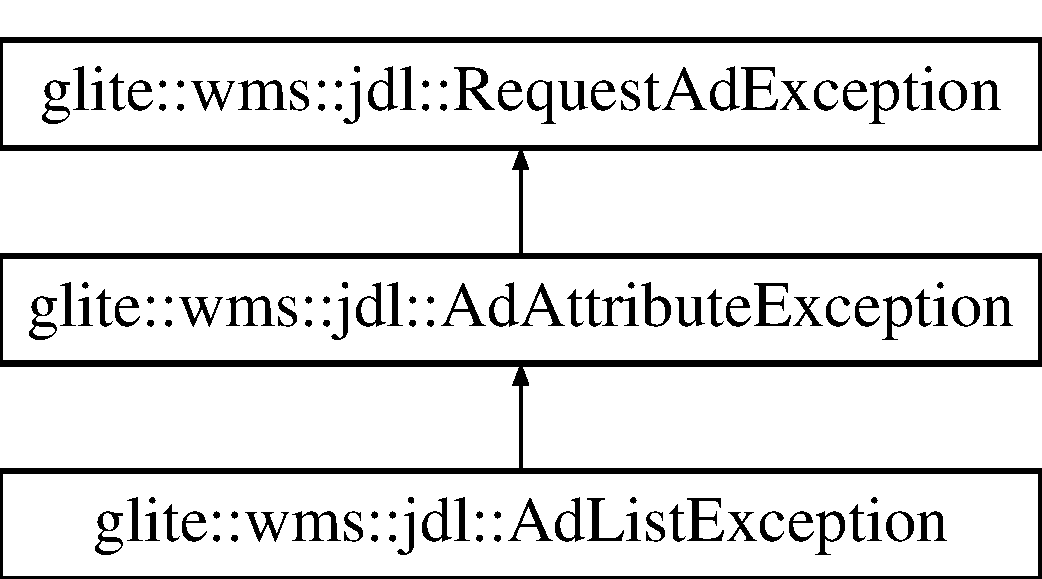
\includegraphics[height=3cm]{classglite_1_1wms_1_1jdl_1_1AdListException}
\end{center}
\end{figure}
\subsection*{Public Member Functions}
\begin{CompactItemize}
\item 
\hyperlink{classglite_1_1wms_1_1jdl_1_1AdListException_a0}{Ad\-List\-Exception} (std::string file, int line, std::string method, int code, std::string attr\_\-name)
\end{CompactItemize}


\subsection{Detailed Description}
\hyperlink{classglite_1_1wms_1_1jdl_1_1AdListException}{Ad\-List\-Exception} - raised when an add method is made on a non-list attribute 



\subsection{Constructor \& Destructor Documentation}
\hypertarget{classglite_1_1wms_1_1jdl_1_1AdListException_a0}{
\index{glite::wms::jdl::AdListException@{glite::wms::jdl::Ad\-List\-Exception}!AdListException@{AdListException}}
\index{AdListException@{AdListException}!glite::wms::jdl::AdListException@{glite::wms::jdl::Ad\-List\-Exception}}
\subsubsection[AdListException]{\setlength{\rightskip}{0pt plus 5cm}glite::wms::jdl::Ad\-List\-Exception::Ad\-List\-Exception (std::string {\em file}, int {\em line}, std::string {\em method}, int {\em code}, std::string {\em attr\_\-name})}}
\label{classglite_1_1wms_1_1jdl_1_1AdListException_a0}


\hyperlink{classglite_1_1wms_1_1jdl_1_1AdListException}{Ad\-List\-Exception} Constructor 

The documentation for this class was generated from the following file:\begin{CompactItemize}
\item 
\hyperlink{RequestAdExceptions_8h}{Request\-Ad\-Exceptions.h}\end{CompactItemize}

\hypertarget{classglite_1_1wms_1_1jdl_1_1AdMismatchException}{
\section{glite::wms::jdl::Ad\-Mismatch\-Exception Class Reference}
\label{classglite_1_1wms_1_1jdl_1_1AdMismatchException}\index{glite::wms::jdl::AdMismatchException@{glite::wms::jdl::AdMismatchException}}
}
{\tt \#include $<$Request\-Ad\-Exceptions.h$>$}

Inheritance diagram for glite::wms::jdl::Ad\-Mismatch\-Exception::\begin{figure}[H]
\begin{center}
\leavevmode
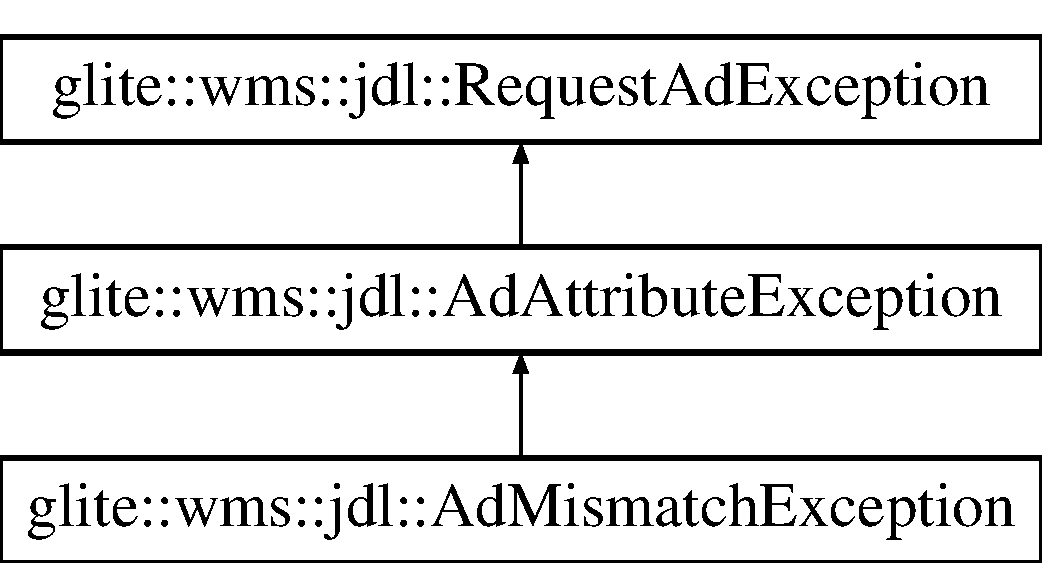
\includegraphics[height=3cm]{classglite_1_1wms_1_1jdl_1_1AdMismatchException}
\end{center}
\end{figure}
\subsection*{Public Member Functions}
\begin{CompactItemize}
\item 
\hyperlink{classglite_1_1wms_1_1jdl_1_1AdMismatchException_a0}{Ad\-Mismatch\-Exception} (std::string file, int line, std::string method, int code, std::string attr\_\-name, std::string \hyperlink{classglite_1_1wms_1_1jdl_1_1RequestAdException_p0}{error\_\-description}=\char`\"{}\char`\"{})
\end{CompactItemize}


\subsection{Detailed Description}
\hyperlink{classglite_1_1wms_1_1jdl_1_1AdMismatchException}{Ad\-Mismatch\-Exception} - raised when a not admitted value is added/set to the jdl 



\subsection{Constructor \& Destructor Documentation}
\hypertarget{classglite_1_1wms_1_1jdl_1_1AdMismatchException_a0}{
\index{glite::wms::jdl::AdMismatchException@{glite::wms::jdl::Ad\-Mismatch\-Exception}!AdMismatchException@{AdMismatchException}}
\index{AdMismatchException@{AdMismatchException}!glite::wms::jdl::AdMismatchException@{glite::wms::jdl::Ad\-Mismatch\-Exception}}
\subsubsection[AdMismatchException]{\setlength{\rightskip}{0pt plus 5cm}glite::wms::jdl::Ad\-Mismatch\-Exception::Ad\-Mismatch\-Exception (std::string {\em file}, int {\em line}, std::string {\em method}, int {\em code}, std::string {\em attr\_\-name}, std::string {\em error\_\-description} = \char`\"{}\char`\"{})}}
\label{classglite_1_1wms_1_1jdl_1_1AdMismatchException_a0}


\hyperlink{classglite_1_1wms_1_1jdl_1_1AdMismatchException}{Ad\-Mismatch\-Exception} Constructor 

The documentation for this class was generated from the following file:\begin{CompactItemize}
\item 
\hyperlink{RequestAdExceptions_8h}{Request\-Ad\-Exceptions.h}\end{CompactItemize}

\hypertarget{classglite_1_1wms_1_1jdl_1_1AdSemanticException}{
\section{glite::wms::jdl::Ad\-Semantic\-Exception Class Reference}
\label{classglite_1_1wms_1_1jdl_1_1AdSemanticException}\index{glite::wms::jdl::AdSemanticException@{glite::wms::jdl::AdSemanticException}}
}
{\tt \#include $<$Request\-Ad\-Exceptions.h$>$}

Inheritance diagram for glite::wms::jdl::Ad\-Semantic\-Exception::\begin{figure}[H]
\begin{center}
\leavevmode
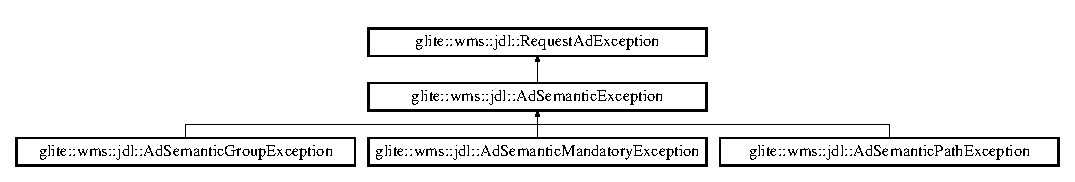
\includegraphics[height=1.99288cm]{classglite_1_1wms_1_1jdl_1_1AdSemanticException}
\end{center}
\end{figure}
\subsection*{Public Member Functions}
\begin{CompactItemize}
\item 
\hyperlink{classglite_1_1wms_1_1jdl_1_1AdSemanticException_a0}{Ad\-Semantic\-Exception::Ad\-Semantic\-Exception} (std::string file, int line, std::string method, int code, std::string exception\_\-name)
\end{CompactItemize}


\subsection{Detailed Description}
\hyperlink{classglite_1_1wms_1_1jdl_1_1AdSemanticException}{Ad\-Semantic\-Exception} - raised while checking the whole constructed \hyperlink{classglite_1_1wms_1_1jdl_1_1JobAd}{Job\-Ad} with the check() method 



\subsection{Member Function Documentation}
\hypertarget{classglite_1_1wms_1_1jdl_1_1AdSemanticException_a0}{
\index{glite::wms::jdl::AdSemanticException@{glite::wms::jdl::Ad\-Semantic\-Exception}!AdSemanticException::AdSemanticException@{AdSemanticException::AdSemanticException}}
\index{AdSemanticException::AdSemanticException@{AdSemanticException::AdSemanticException}!glite::wms::jdl::AdSemanticException@{glite::wms::jdl::Ad\-Semantic\-Exception}}
\subsubsection[AdSemanticException::AdSemanticException]{\setlength{\rightskip}{0pt plus 5cm}glite::wms::jdl::Ad\-Semantic\-Exception::Ad\-Semantic\-Exception::Ad\-Semantic\-Exception (std::string {\em file}, int {\em line}, std::string {\em method}, int {\em code}, std::string {\em exception\_\-name})}}
\label{classglite_1_1wms_1_1jdl_1_1AdSemanticException_a0}


Raised when mandatory attribute is missing, unable to find a specified path, wrong attribute coexistence 

The documentation for this class was generated from the following file:\begin{CompactItemize}
\item 
\hyperlink{RequestAdExceptions_8h}{Request\-Ad\-Exceptions.h}\end{CompactItemize}

\hypertarget{classglite_1_1wms_1_1jdl_1_1AdSemanticGroupException}{
\section{glite::wms::jdl::Ad\-Semantic\-Group\-Exception Class Reference}
\label{classglite_1_1wms_1_1jdl_1_1AdSemanticGroupException}\index{glite::wms::jdl::AdSemanticGroupException@{glite::wms::jdl::AdSemanticGroupException}}
}
{\tt \#include $<$Request\-Ad\-Exceptions.h$>$}

Inheritance diagram for glite::wms::jdl::Ad\-Semantic\-Group\-Exception::\begin{figure}[H]
\begin{center}
\leavevmode
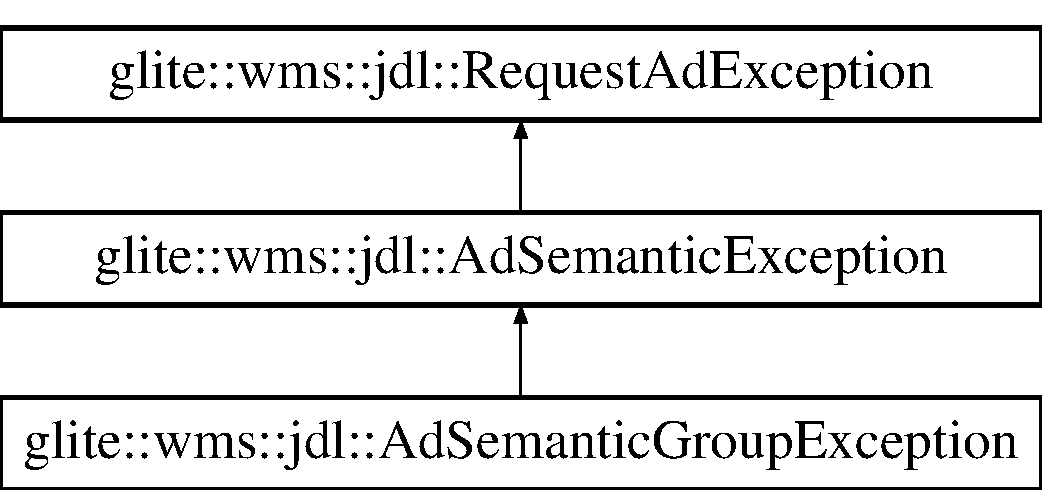
\includegraphics[height=3cm]{classglite_1_1wms_1_1jdl_1_1AdSemanticGroupException}
\end{center}
\end{figure}
\subsection*{Public Member Functions}
\begin{CompactItemize}
\item 
\hyperlink{classglite_1_1wms_1_1jdl_1_1AdSemanticGroupException_a0}{Ad\-Semantic\-Group\-Exception} (std::string file, int line, std::string method, int code, std::string attrs\_\-name)
\end{CompactItemize}


\subsection{Detailed Description}
\hyperlink{classglite_1_1wms_1_1jdl_1_1AdSemanticGroupException}{Ad\-Semantic\-Group\-Exception} - raised when a mandatoty attribute is missing to the class\-Ad 



\subsection{Constructor \& Destructor Documentation}
\hypertarget{classglite_1_1wms_1_1jdl_1_1AdSemanticGroupException_a0}{
\index{glite::wms::jdl::AdSemanticGroupException@{glite::wms::jdl::Ad\-Semantic\-Group\-Exception}!AdSemanticGroupException@{AdSemanticGroupException}}
\index{AdSemanticGroupException@{AdSemanticGroupException}!glite::wms::jdl::AdSemanticGroupException@{glite::wms::jdl::Ad\-Semantic\-Group\-Exception}}
\subsubsection[AdSemanticGroupException]{\setlength{\rightskip}{0pt plus 5cm}glite::wms::jdl::Ad\-Semantic\-Group\-Exception::Ad\-Semantic\-Group\-Exception (std::string {\em file}, int {\em line}, std::string {\em method}, int {\em code}, std::string {\em attrs\_\-name})}}
\label{classglite_1_1wms_1_1jdl_1_1AdSemanticGroupException_a0}


Raised when Group attribute is missing, unable to find a specified path, wrong attribute coexistence 

The documentation for this class was generated from the following file:\begin{CompactItemize}
\item 
\hyperlink{RequestAdExceptions_8h}{Request\-Ad\-Exceptions.h}\end{CompactItemize}

\hypertarget{classglite_1_1wms_1_1jdl_1_1AdSemanticMandatoryException}{
\section{glite::wms::jdl::Ad\-Semantic\-Mandatory\-Exception Class Reference}
\label{classglite_1_1wms_1_1jdl_1_1AdSemanticMandatoryException}\index{glite::wms::jdl::AdSemanticMandatoryException@{glite::wms::jdl::AdSemanticMandatoryException}}
}
{\tt \#include $<$Request\-Ad\-Exceptions.h$>$}

Inheritance diagram for glite::wms::jdl::Ad\-Semantic\-Mandatory\-Exception::\begin{figure}[H]
\begin{center}
\leavevmode
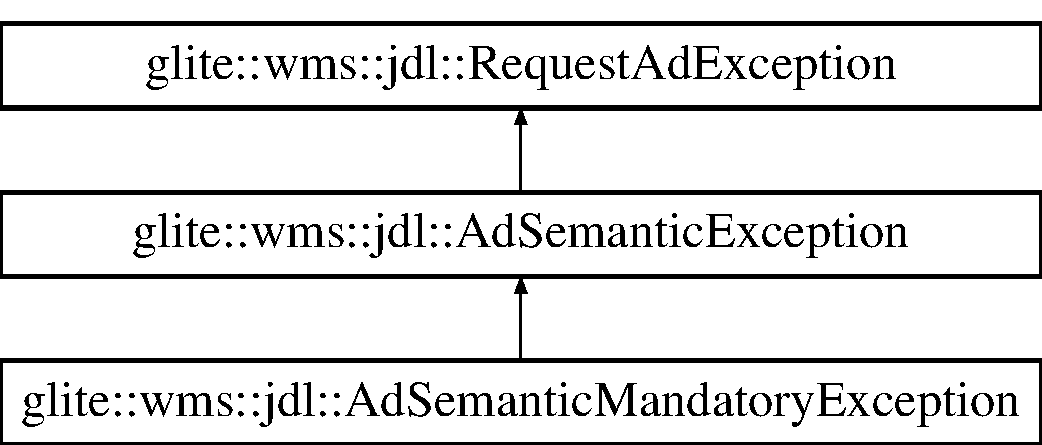
\includegraphics[height=3cm]{classglite_1_1wms_1_1jdl_1_1AdSemanticMandatoryException}
\end{center}
\end{figure}
\subsection*{Public Member Functions}
\begin{CompactItemize}
\item 
\hyperlink{classglite_1_1wms_1_1jdl_1_1AdSemanticMandatoryException_a0}{Ad\-Semantic\-Mandatory\-Exception} (std::string file, int line, std::string method, int code, std::string attr\_\-name)
\end{CompactItemize}


\subsection{Detailed Description}
\hyperlink{classglite_1_1wms_1_1jdl_1_1AdSemanticMandatoryException}{Ad\-Semantic\-Mandatory\-Exception} - raised when a mandatoty attribute is missing to the class\-Ad 



\subsection{Constructor \& Destructor Documentation}
\hypertarget{classglite_1_1wms_1_1jdl_1_1AdSemanticMandatoryException_a0}{
\index{glite::wms::jdl::AdSemanticMandatoryException@{glite::wms::jdl::Ad\-Semantic\-Mandatory\-Exception}!AdSemanticMandatoryException@{AdSemanticMandatoryException}}
\index{AdSemanticMandatoryException@{AdSemanticMandatoryException}!glite::wms::jdl::AdSemanticMandatoryException@{glite::wms::jdl::Ad\-Semantic\-Mandatory\-Exception}}
\subsubsection[AdSemanticMandatoryException]{\setlength{\rightskip}{0pt plus 5cm}glite::wms::jdl::Ad\-Semantic\-Mandatory\-Exception::Ad\-Semantic\-Mandatory\-Exception (std::string {\em file}, int {\em line}, std::string {\em method}, int {\em code}, std::string {\em attr\_\-name})}}
\label{classglite_1_1wms_1_1jdl_1_1AdSemanticMandatoryException_a0}


Raised when mandatory attribute is missing, unable to find a specified path, wrong attribute coexistence 

The documentation for this class was generated from the following file:\begin{CompactItemize}
\item 
\hyperlink{RequestAdExceptions_8h}{Request\-Ad\-Exceptions.h}\end{CompactItemize}

\hypertarget{classglite_1_1wms_1_1jdl_1_1AdSemanticPathException}{
\section{glite::wms::jdl::Ad\-Semantic\-Path\-Exception Class Reference}
\label{classglite_1_1wms_1_1jdl_1_1AdSemanticPathException}\index{glite::wms::jdl::AdSemanticPathException@{glite::wms::jdl::AdSemanticPathException}}
}
{\tt \#include $<$Request\-Ad\-Exceptions.h$>$}

Inheritance diagram for glite::wms::jdl::Ad\-Semantic\-Path\-Exception::\begin{figure}[H]
\begin{center}
\leavevmode
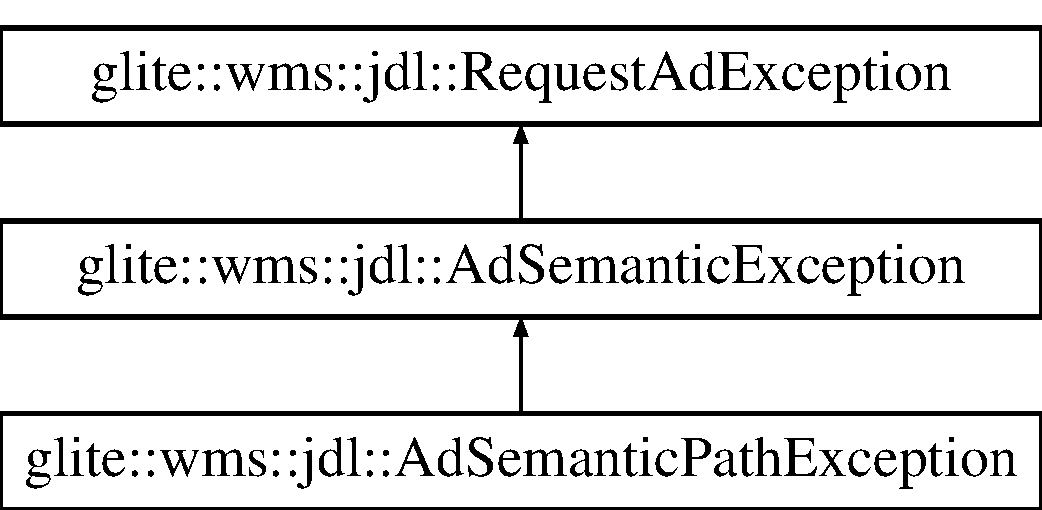
\includegraphics[height=3cm]{classglite_1_1wms_1_1jdl_1_1AdSemanticPathException}
\end{center}
\end{figure}
\subsection*{Public Member Functions}
\begin{CompactItemize}
\item 
\hyperlink{classglite_1_1wms_1_1jdl_1_1AdSemanticPathException_a0}{Ad\-Semantic\-Path\-Exception} (std::string file, int line, std::string method, int code, std::string attr\_\-name, std::string path\_\-name)
\end{CompactItemize}


\subsection{Detailed Description}
\hyperlink{classglite_1_1wms_1_1jdl_1_1AdSemanticPathException}{Ad\-Semantic\-Path\-Exception} - raised when a mandatoty attribute is missing to the class\-Ad 



\subsection{Constructor \& Destructor Documentation}
\hypertarget{classglite_1_1wms_1_1jdl_1_1AdSemanticPathException_a0}{
\index{glite::wms::jdl::AdSemanticPathException@{glite::wms::jdl::Ad\-Semantic\-Path\-Exception}!AdSemanticPathException@{AdSemanticPathException}}
\index{AdSemanticPathException@{AdSemanticPathException}!glite::wms::jdl::AdSemanticPathException@{glite::wms::jdl::Ad\-Semantic\-Path\-Exception}}
\subsubsection[AdSemanticPathException]{\setlength{\rightskip}{0pt plus 5cm}glite::wms::jdl::Ad\-Semantic\-Path\-Exception::Ad\-Semantic\-Path\-Exception (std::string {\em file}, int {\em line}, std::string {\em method}, int {\em code}, std::string {\em attr\_\-name}, std::string {\em path\_\-name})}}
\label{classglite_1_1wms_1_1jdl_1_1AdSemanticPathException_a0}


Raised when Path attribute is missing, unable to find a specified path, wrong attribute coexistence 

The documentation for this class was generated from the following file:\begin{CompactItemize}
\item 
\hyperlink{RequestAdExceptions_8h}{Request\-Ad\-Exceptions.h}\end{CompactItemize}

\hypertarget{classglite_1_1wms_1_1jdl_1_1AdSyntaxException}{
\section{glite::wms::jdl::Ad\-Syntax\-Exception Class Reference}
\label{classglite_1_1wms_1_1jdl_1_1AdSyntaxException}\index{glite::wms::jdl::AdSyntaxException@{glite::wms::jdl::AdSyntaxException}}
}
{\tt \#include $<$Request\-Ad\-Exceptions.h$>$}

Inheritance diagram for glite::wms::jdl::Ad\-Syntax\-Exception::\begin{figure}[H]
\begin{center}
\leavevmode
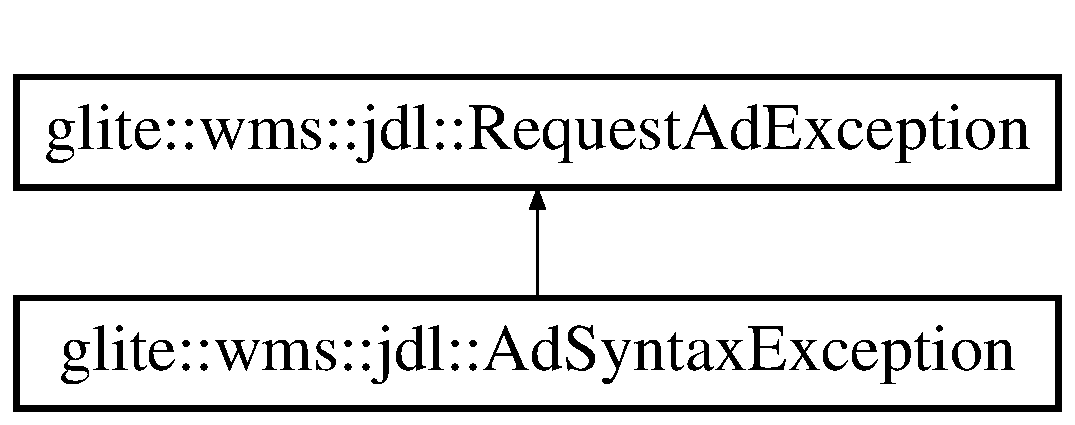
\includegraphics[height=2cm]{classglite_1_1wms_1_1jdl_1_1AdSyntaxException}
\end{center}
\end{figure}
\subsection*{Public Member Functions}
\begin{CompactItemize}
\item 
\hyperlink{classglite_1_1wms_1_1jdl_1_1AdSyntaxException_a0}{Ad\-Syntax\-Exception::Ad\-Syntax\-Exception} (std::string file, int line, std::string method, int code, std::string attr\_\-name)
\end{CompactItemize}


\subsection{Detailed Description}
\hyperlink{classglite_1_1wms_1_1jdl_1_1AdSyntaxException}{Ad\-Syntax\-Exception} - raised when syntax error is checked during add/set methods 



\subsection{Member Function Documentation}
\hypertarget{classglite_1_1wms_1_1jdl_1_1AdSyntaxException_a0}{
\index{glite::wms::jdl::AdSyntaxException@{glite::wms::jdl::Ad\-Syntax\-Exception}!AdSyntaxException::AdSyntaxException@{AdSyntaxException::AdSyntaxException}}
\index{AdSyntaxException::AdSyntaxException@{AdSyntaxException::AdSyntaxException}!glite::wms::jdl::AdSyntaxException@{glite::wms::jdl::Ad\-Syntax\-Exception}}
\subsubsection[AdSyntaxException::AdSyntaxException]{\setlength{\rightskip}{0pt plus 5cm}glite::wms::jdl::Ad\-Syntax\-Exception::Ad\-Syntax\-Exception::Ad\-Syntax\-Exception (std::string {\em file}, int {\em line}, std::string {\em method}, int {\em code}, std::string {\em attr\_\-name})}}
\label{classglite_1_1wms_1_1jdl_1_1AdSyntaxException_a0}




The documentation for this class was generated from the following file:\begin{CompactItemize}
\item 
\hyperlink{RequestAdExceptions_8h}{Request\-Ad\-Exceptions.h}\end{CompactItemize}

\hypertarget{classglite_1_1wms_1_1jdl_1_1CannotGetAttribute}{
\section{glite::wms::jdl::Cannot\-Get\-Attribute Class Reference}
\label{classglite_1_1wms_1_1jdl_1_1CannotGetAttribute}\index{glite::wms::jdl::CannotGetAttribute@{glite::wms::jdl::CannotGetAttribute}}
}
{\tt \#include $<$Manipulation\-Exceptions.h$>$}

Inheritance diagram for glite::wms::jdl::Cannot\-Get\-Attribute::\begin{figure}[H]
\begin{center}
\leavevmode
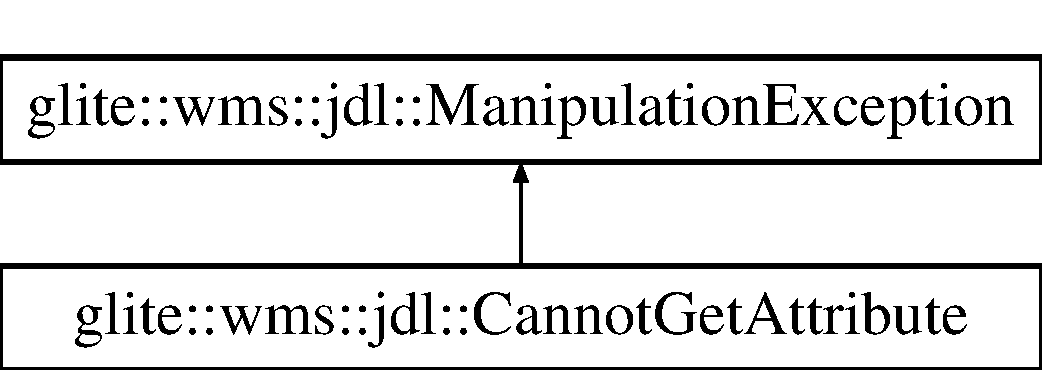
\includegraphics[height=2cm]{classglite_1_1wms_1_1jdl_1_1CannotGetAttribute}
\end{center}
\end{figure}
\subsection*{Public Member Functions}
\begin{CompactItemize}
\item 
\hyperlink{classglite_1_1wms_1_1jdl_1_1CannotGetAttribute_a0}{Cannot\-Get\-Attribute} (const std::string \&parameter)
\item 
virtual \hyperlink{classglite_1_1wms_1_1jdl_1_1CannotGetAttribute_a1}{$\sim$Cannot\-Get\-Attribute} (void)  throw ()
\item 
virtual std::string \hyperlink{classglite_1_1wms_1_1jdl_1_1CannotGetAttribute_a2}{reason} (void) const 
\end{CompactItemize}


\subsection{Constructor \& Destructor Documentation}
\hypertarget{classglite_1_1wms_1_1jdl_1_1CannotGetAttribute_a0}{
\index{glite::wms::jdl::CannotGetAttribute@{glite::wms::jdl::Cannot\-Get\-Attribute}!CannotGetAttribute@{CannotGetAttribute}}
\index{CannotGetAttribute@{CannotGetAttribute}!glite::wms::jdl::CannotGetAttribute@{glite::wms::jdl::Cannot\-Get\-Attribute}}
\subsubsection[CannotGetAttribute]{\setlength{\rightskip}{0pt plus 5cm}glite::wms::jdl::Cannot\-Get\-Attribute::Cannot\-Get\-Attribute (const std::string \& {\em parameter})\hspace{0.3cm}{\tt  \mbox{[}explicit\mbox{]}}}}
\label{classglite_1_1wms_1_1jdl_1_1CannotGetAttribute_a0}


\hypertarget{classglite_1_1wms_1_1jdl_1_1CannotGetAttribute_a1}{
\index{glite::wms::jdl::CannotGetAttribute@{glite::wms::jdl::Cannot\-Get\-Attribute}!~CannotGetAttribute@{$\sim$CannotGetAttribute}}
\index{~CannotGetAttribute@{$\sim$CannotGetAttribute}!glite::wms::jdl::CannotGetAttribute@{glite::wms::jdl::Cannot\-Get\-Attribute}}
\subsubsection[$\sim$CannotGetAttribute]{\setlength{\rightskip}{0pt plus 5cm}virtual glite::wms::jdl::Cannot\-Get\-Attribute::$\sim$\hyperlink{classglite_1_1wms_1_1jdl_1_1CannotGetAttribute}{Cannot\-Get\-Attribute} (void)  throw ()\hspace{0.3cm}{\tt  \mbox{[}virtual\mbox{]}}}}
\label{classglite_1_1wms_1_1jdl_1_1CannotGetAttribute_a1}




\subsection{Member Function Documentation}
\hypertarget{classglite_1_1wms_1_1jdl_1_1CannotGetAttribute_a2}{
\index{glite::wms::jdl::CannotGetAttribute@{glite::wms::jdl::Cannot\-Get\-Attribute}!reason@{reason}}
\index{reason@{reason}!glite::wms::jdl::CannotGetAttribute@{glite::wms::jdl::Cannot\-Get\-Attribute}}
\subsubsection[reason]{\setlength{\rightskip}{0pt plus 5cm}virtual std::string glite::wms::jdl::Cannot\-Get\-Attribute::reason (void) const\hspace{0.3cm}{\tt  \mbox{[}virtual\mbox{]}}}}
\label{classglite_1_1wms_1_1jdl_1_1CannotGetAttribute_a2}




Reimplemented from \hyperlink{classglite_1_1wms_1_1jdl_1_1ManipulationException_a4}{glite::wms::jdl::Manipulation\-Exception}.

The documentation for this class was generated from the following file:\begin{CompactItemize}
\item 
\hyperlink{ManipulationExceptions_8h}{Manipulation\-Exceptions.h}\end{CompactItemize}

\hypertarget{classglite_1_1wms_1_1jdl_1_1CannotRemoveAttribute}{
\section{glite::wms::jdl::Cannot\-Remove\-Attribute Class Reference}
\label{classglite_1_1wms_1_1jdl_1_1CannotRemoveAttribute}\index{glite::wms::jdl::CannotRemoveAttribute@{glite::wms::jdl::CannotRemoveAttribute}}
}
{\tt \#include $<$Manipulation\-Exceptions.h$>$}

Inheritance diagram for glite::wms::jdl::Cannot\-Remove\-Attribute::\begin{figure}[H]
\begin{center}
\leavevmode
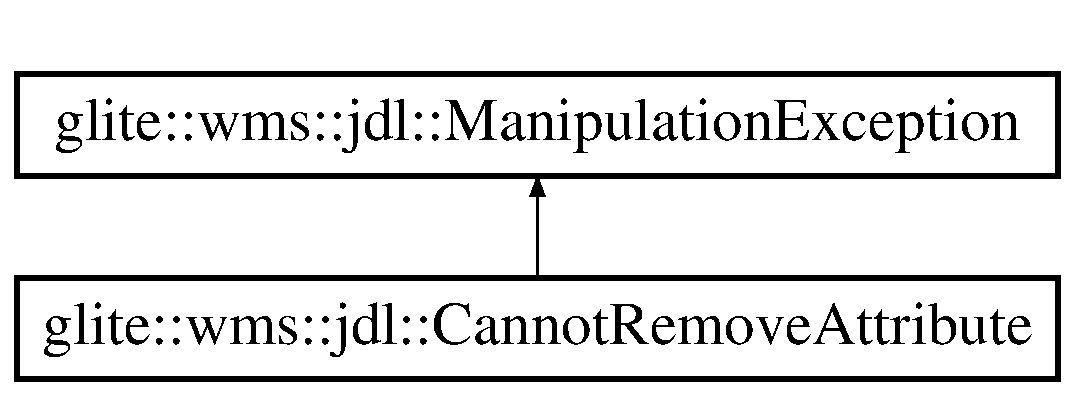
\includegraphics[height=2cm]{classglite_1_1wms_1_1jdl_1_1CannotRemoveAttribute}
\end{center}
\end{figure}
\subsection*{Public Member Functions}
\begin{CompactItemize}
\item 
\hyperlink{classglite_1_1wms_1_1jdl_1_1CannotRemoveAttribute_a0}{Cannot\-Remove\-Attribute} (const std::string \&parameter)
\item 
virtual \hyperlink{classglite_1_1wms_1_1jdl_1_1CannotRemoveAttribute_a1}{$\sim$Cannot\-Remove\-Attribute} (void)  throw ()
\item 
virtual std::string \hyperlink{classglite_1_1wms_1_1jdl_1_1CannotRemoveAttribute_a2}{reason} (void) const 
\end{CompactItemize}


\subsection{Constructor \& Destructor Documentation}
\hypertarget{classglite_1_1wms_1_1jdl_1_1CannotRemoveAttribute_a0}{
\index{glite::wms::jdl::CannotRemoveAttribute@{glite::wms::jdl::Cannot\-Remove\-Attribute}!CannotRemoveAttribute@{CannotRemoveAttribute}}
\index{CannotRemoveAttribute@{CannotRemoveAttribute}!glite::wms::jdl::CannotRemoveAttribute@{glite::wms::jdl::Cannot\-Remove\-Attribute}}
\subsubsection[CannotRemoveAttribute]{\setlength{\rightskip}{0pt plus 5cm}glite::wms::jdl::Cannot\-Remove\-Attribute::Cannot\-Remove\-Attribute (const std::string \& {\em parameter})\hspace{0.3cm}{\tt  \mbox{[}explicit\mbox{]}}}}
\label{classglite_1_1wms_1_1jdl_1_1CannotRemoveAttribute_a0}


\hypertarget{classglite_1_1wms_1_1jdl_1_1CannotRemoveAttribute_a1}{
\index{glite::wms::jdl::CannotRemoveAttribute@{glite::wms::jdl::Cannot\-Remove\-Attribute}!~CannotRemoveAttribute@{$\sim$CannotRemoveAttribute}}
\index{~CannotRemoveAttribute@{$\sim$CannotRemoveAttribute}!glite::wms::jdl::CannotRemoveAttribute@{glite::wms::jdl::Cannot\-Remove\-Attribute}}
\subsubsection[$\sim$CannotRemoveAttribute]{\setlength{\rightskip}{0pt plus 5cm}virtual glite::wms::jdl::Cannot\-Remove\-Attribute::$\sim$\hyperlink{classglite_1_1wms_1_1jdl_1_1CannotRemoveAttribute}{Cannot\-Remove\-Attribute} (void)  throw ()\hspace{0.3cm}{\tt  \mbox{[}virtual\mbox{]}}}}
\label{classglite_1_1wms_1_1jdl_1_1CannotRemoveAttribute_a1}




\subsection{Member Function Documentation}
\hypertarget{classglite_1_1wms_1_1jdl_1_1CannotRemoveAttribute_a2}{
\index{glite::wms::jdl::CannotRemoveAttribute@{glite::wms::jdl::Cannot\-Remove\-Attribute}!reason@{reason}}
\index{reason@{reason}!glite::wms::jdl::CannotRemoveAttribute@{glite::wms::jdl::Cannot\-Remove\-Attribute}}
\subsubsection[reason]{\setlength{\rightskip}{0pt plus 5cm}virtual std::string glite::wms::jdl::Cannot\-Remove\-Attribute::reason (void) const\hspace{0.3cm}{\tt  \mbox{[}virtual\mbox{]}}}}
\label{classglite_1_1wms_1_1jdl_1_1CannotRemoveAttribute_a2}




Reimplemented from \hyperlink{classglite_1_1wms_1_1jdl_1_1ManipulationException_a4}{glite::wms::jdl::Manipulation\-Exception}.

The documentation for this class was generated from the following file:\begin{CompactItemize}
\item 
\hyperlink{ManipulationExceptions_8h}{Manipulation\-Exceptions.h}\end{CompactItemize}

\hypertarget{classglite_1_1wms_1_1jdl_1_1CannotSetAttribute}{
\section{glite::wms::jdl::Cannot\-Set\-Attribute Class Reference}
\label{classglite_1_1wms_1_1jdl_1_1CannotSetAttribute}\index{glite::wms::jdl::CannotSetAttribute@{glite::wms::jdl::CannotSetAttribute}}
}
{\tt \#include $<$Manipulation\-Exceptions.h$>$}

Inheritance diagram for glite::wms::jdl::Cannot\-Set\-Attribute::\begin{figure}[H]
\begin{center}
\leavevmode
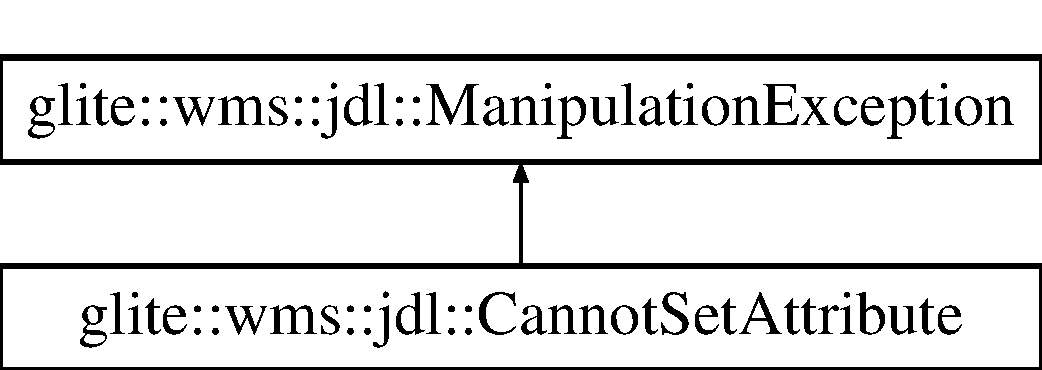
\includegraphics[height=2cm]{classglite_1_1wms_1_1jdl_1_1CannotSetAttribute}
\end{center}
\end{figure}
\subsection*{Public Member Functions}
\begin{CompactItemize}
\item 
\hyperlink{classglite_1_1wms_1_1jdl_1_1CannotSetAttribute_a0}{Cannot\-Set\-Attribute} (const std::string \&parameter)
\item 
virtual \hyperlink{classglite_1_1wms_1_1jdl_1_1CannotSetAttribute_a1}{$\sim$Cannot\-Set\-Attribute} (void)  throw ()
\item 
virtual std::string \hyperlink{classglite_1_1wms_1_1jdl_1_1CannotSetAttribute_a2}{reason} (void) const 
\end{CompactItemize}


\subsection{Constructor \& Destructor Documentation}
\hypertarget{classglite_1_1wms_1_1jdl_1_1CannotSetAttribute_a0}{
\index{glite::wms::jdl::CannotSetAttribute@{glite::wms::jdl::Cannot\-Set\-Attribute}!CannotSetAttribute@{CannotSetAttribute}}
\index{CannotSetAttribute@{CannotSetAttribute}!glite::wms::jdl::CannotSetAttribute@{glite::wms::jdl::Cannot\-Set\-Attribute}}
\subsubsection[CannotSetAttribute]{\setlength{\rightskip}{0pt plus 5cm}glite::wms::jdl::Cannot\-Set\-Attribute::Cannot\-Set\-Attribute (const std::string \& {\em parameter})\hspace{0.3cm}{\tt  \mbox{[}explicit\mbox{]}}}}
\label{classglite_1_1wms_1_1jdl_1_1CannotSetAttribute_a0}


\hypertarget{classglite_1_1wms_1_1jdl_1_1CannotSetAttribute_a1}{
\index{glite::wms::jdl::CannotSetAttribute@{glite::wms::jdl::Cannot\-Set\-Attribute}!~CannotSetAttribute@{$\sim$CannotSetAttribute}}
\index{~CannotSetAttribute@{$\sim$CannotSetAttribute}!glite::wms::jdl::CannotSetAttribute@{glite::wms::jdl::Cannot\-Set\-Attribute}}
\subsubsection[$\sim$CannotSetAttribute]{\setlength{\rightskip}{0pt plus 5cm}virtual glite::wms::jdl::Cannot\-Set\-Attribute::$\sim$\hyperlink{classglite_1_1wms_1_1jdl_1_1CannotSetAttribute}{Cannot\-Set\-Attribute} (void)  throw ()\hspace{0.3cm}{\tt  \mbox{[}virtual\mbox{]}}}}
\label{classglite_1_1wms_1_1jdl_1_1CannotSetAttribute_a1}




\subsection{Member Function Documentation}
\hypertarget{classglite_1_1wms_1_1jdl_1_1CannotSetAttribute_a2}{
\index{glite::wms::jdl::CannotSetAttribute@{glite::wms::jdl::Cannot\-Set\-Attribute}!reason@{reason}}
\index{reason@{reason}!glite::wms::jdl::CannotSetAttribute@{glite::wms::jdl::Cannot\-Set\-Attribute}}
\subsubsection[reason]{\setlength{\rightskip}{0pt plus 5cm}virtual std::string glite::wms::jdl::Cannot\-Set\-Attribute::reason (void) const\hspace{0.3cm}{\tt  \mbox{[}virtual\mbox{]}}}}
\label{classglite_1_1wms_1_1jdl_1_1CannotSetAttribute_a2}




Reimplemented from \hyperlink{classglite_1_1wms_1_1jdl_1_1ManipulationException_a4}{glite::wms::jdl::Manipulation\-Exception}.

The documentation for this class was generated from the following file:\begin{CompactItemize}
\item 
\hyperlink{ManipulationExceptions_8h}{Manipulation\-Exceptions.h}\end{CompactItemize}

\hypertarget{classglite_1_1wms_1_1jdl_1_1DAGAd}{
\section{glite::wms::jdl::DAGAd Class Reference}
\label{classglite_1_1wms_1_1jdl_1_1DAGAd}\index{glite::wms::jdl::DAGAd@{glite::wms::jdl::DAGAd}}
}
{\tt \#include $<$DAGAd.h$>$}

\subsection*{Public Types}
\begin{CompactItemize}
\item 
typedef \hyperlink{classglite_1_1wms_1_1jdl_1_1DAGAdNodeIterator}{DAGAd\-Node\-Iterator} \hyperlink{classglite_1_1wms_1_1jdl_1_1DAGAd_w0}{node\_\-iterator}
\item 
typedef DAGAd\-Node\-Iterator::value\_\-type \hyperlink{classglite_1_1wms_1_1jdl_1_1DAGAd_w1}{node\_\-value\_\-type}
\item 
typedef \hyperlink{structglite_1_1wms_1_1jdl_1_1DAGAdDependencyIterator}{DAGAd\-Dependency\-Iterator} \hyperlink{classglite_1_1wms_1_1jdl_1_1DAGAd_w2}{dependency\_\-iterator}
\item 
typedef DAGAd\-Dependency\-Iterator::value\_\-type \hyperlink{classglite_1_1wms_1_1jdl_1_1DAGAd_w3}{dependency\_\-value\_\-type}
\item 
typedef boost::adjacency\_\-list$<$ boost::vec\-S, boost::vec\-S, boost::directed\-S $>$ \hyperlink{classglite_1_1wms_1_1jdl_1_1DAGAd_w4}{Graph\_\-t}
\item 
typedef boost::graph\_\-traits$<$ \hyperlink{classglite_1_1wms_1_1jdl_1_1DAGAd_w4}{Graph\_\-t} $>$::vertex\_\-descriptor \hyperlink{classglite_1_1wms_1_1jdl_1_1DAGAd_w5}{Vertex}
\item 
typedef boost::property\_\-map$<$ \hyperlink{classglite_1_1wms_1_1jdl_1_1DAGAd_w4}{Graph\_\-t}, boost::vertex\_\-color\_\-t $>$::type \hyperlink{classglite_1_1wms_1_1jdl_1_1DAGAd_w6}{Color}
\item 
typedef std::map$<$ std::string, \hyperlink{classglite_1_1wms_1_1jdl_1_1DAGAd_w5}{Vertex} $>$ \hyperlink{classglite_1_1wms_1_1jdl_1_1DAGAd_w7}{Mapping}
\end{CompactItemize}
\subsection*{Public Member Functions}
\begin{CompactItemize}
\item 
\hyperlink{classglite_1_1wms_1_1jdl_1_1DAGAd_a0}{DAGAd} ()
\item 
\hyperlink{classglite_1_1wms_1_1jdl_1_1DAGAd_a1}{DAGAd} (classad::Class\-Ad const \&ad)
\item 
classad::Class\-Ad const \& \hyperlink{classglite_1_1wms_1_1jdl_1_1DAGAd_a2}{ad} () const 
\item 
int \hyperlink{classglite_1_1wms_1_1jdl_1_1DAGAd_a3}{max\_\-running\_\-nodes} (int new\_\-value)
\item 
int \hyperlink{classglite_1_1wms_1_1jdl_1_1DAGAd_a4}{max\_\-running\_\-nodes} () const 
\item 
std::string \hyperlink{classglite_1_1wms_1_1jdl_1_1DAGAd_a5}{default\_\-node\_\-type} (std::string const \&new\_\-value)
\item 
std::string \hyperlink{classglite_1_1wms_1_1jdl_1_1DAGAd_a6}{default\_\-node\_\-type} () const 
\item 
int \hyperlink{classglite_1_1wms_1_1jdl_1_1DAGAd_a7}{default\_\-node\_\-retry\_\-count} (int new\_\-value)
\item 
int \hyperlink{classglite_1_1wms_1_1jdl_1_1DAGAd_a8}{default\_\-node\_\-retry\_\-count} () const 
\item 
bool \hyperlink{classglite_1_1wms_1_1jdl_1_1DAGAd_a9}{add\_\-node} (std::string const \&name, \hyperlink{classglite_1_1wms_1_1jdl_1_1DAGNodeInfo}{DAGNode\-Info} const \&info)
\item 
bool \hyperlink{classglite_1_1wms_1_1jdl_1_1DAGAd_a10}{replace\_\-node} (std::string const \&name, \hyperlink{classglite_1_1wms_1_1jdl_1_1DAGNodeInfo}{DAGNode\-Info} const \&info)
\item 
bool \hyperlink{classglite_1_1wms_1_1jdl_1_1DAGAd_a11}{remove\_\-node} (std::string const \&name)
\item 
std::size\_\-t \hyperlink{classglite_1_1wms_1_1jdl_1_1DAGAd_a12}{num\_\-nodes} () const 
\item 
\hyperlink{classglite_1_1wms_1_1jdl_1_1DAGAdNodeIterator}{node\_\-iterator} \hyperlink{classglite_1_1wms_1_1jdl_1_1DAGAd_a13}{find} (std::string const \&name) const 
\item 
bool \hyperlink{classglite_1_1wms_1_1jdl_1_1DAGAd_a14}{add\_\-dependency} (std::string const \&first, std::string const \&second)
\item 
bool \hyperlink{classglite_1_1wms_1_1jdl_1_1DAGAd_a15}{remove\_\-dependency} (std::string const \&first, std::string const \&second)
\item 
std::size\_\-t \hyperlink{classglite_1_1wms_1_1jdl_1_1DAGAd_a16}{num\_\-dependencies} () const 
\item 
bool \hyperlink{classglite_1_1wms_1_1jdl_1_1DAGAd_a17}{set\_\-generic} (std::string const \&attribute, classad::Expr\-Tree $\ast$value)
\item 
classad::Expr\-Tree const $\ast$ \hyperlink{classglite_1_1wms_1_1jdl_1_1DAGAd_a18}{get\_\-generic} (std::string const \&attribute) const 
\item 
bool \hyperlink{classglite_1_1wms_1_1jdl_1_1DAGAd_a19}{remove\_\-generic} (std::string const \&attribute)
\item 
std::pair$<$ \hyperlink{structglite_1_1wms_1_1jdl_1_1DAGAdDependencyIterator}{dependency\_\-iterator}, \hyperlink{structglite_1_1wms_1_1jdl_1_1DAGAdDependencyIterator}{dependency\_\-iterator} $>$ \hyperlink{classglite_1_1wms_1_1jdl_1_1DAGAd_a20}{dependencies} () const 
\item 
std::pair$<$ \hyperlink{classglite_1_1wms_1_1jdl_1_1DAGAdNodeIterator}{node\_\-iterator}, \hyperlink{classglite_1_1wms_1_1jdl_1_1DAGAdNodeIterator}{node\_\-iterator} $>$ \hyperlink{classglite_1_1wms_1_1jdl_1_1DAGAd_a21}{nodes} () const 
\end{CompactItemize}


\subsection{Member Typedef Documentation}
\hypertarget{classglite_1_1wms_1_1jdl_1_1DAGAd_w6}{
\index{glite::wms::jdl::DAGAd@{glite::wms::jdl::DAGAd}!Color@{Color}}
\index{Color@{Color}!glite::wms::jdl::DAGAd@{glite::wms::jdl::DAGAd}}
\subsubsection[Color]{\setlength{\rightskip}{0pt plus 5cm}typedef boost::property\_\-map$<$\hyperlink{classglite_1_1wms_1_1jdl_1_1DAGAd_w4}{Graph\_\-t}, boost::vertex\_\-color\_\-t$>$::type \hyperlink{classglite_1_1wms_1_1jdl_1_1DAGAd_w6}{glite::wms::jdl::DAGAd::Color}}}
\label{classglite_1_1wms_1_1jdl_1_1DAGAd_w6}


\hypertarget{classglite_1_1wms_1_1jdl_1_1DAGAd_w2}{
\index{glite::wms::jdl::DAGAd@{glite::wms::jdl::DAGAd}!dependency_iterator@{dependency\_\-iterator}}
\index{dependency_iterator@{dependency\_\-iterator}!glite::wms::jdl::DAGAd@{glite::wms::jdl::DAGAd}}
\subsubsection[dependency\_\-iterator]{\setlength{\rightskip}{0pt plus 5cm}typedef \hyperlink{structglite_1_1wms_1_1jdl_1_1DAGAdDependencyIterator}{DAGAd\-Dependency\-Iterator} \hyperlink{structglite_1_1wms_1_1jdl_1_1DAGAdDependencyIterator}{glite::wms::jdl::DAGAd::dependency\_\-iterator}}}
\label{classglite_1_1wms_1_1jdl_1_1DAGAd_w2}


\hypertarget{classglite_1_1wms_1_1jdl_1_1DAGAd_w3}{
\index{glite::wms::jdl::DAGAd@{glite::wms::jdl::DAGAd}!dependency_value_type@{dependency\_\-value\_\-type}}
\index{dependency_value_type@{dependency\_\-value\_\-type}!glite::wms::jdl::DAGAd@{glite::wms::jdl::DAGAd}}
\subsubsection[dependency\_\-value\_\-type]{\setlength{\rightskip}{0pt plus 5cm}typedef DAGAd\-Dependency\-Iterator::value\_\-type \hyperlink{classglite_1_1wms_1_1jdl_1_1DAGAd_w3}{glite::wms::jdl::DAGAd::dependency\_\-value\_\-type}}}
\label{classglite_1_1wms_1_1jdl_1_1DAGAd_w3}


\hypertarget{classglite_1_1wms_1_1jdl_1_1DAGAd_w4}{
\index{glite::wms::jdl::DAGAd@{glite::wms::jdl::DAGAd}!Graph_t@{Graph\_\-t}}
\index{Graph_t@{Graph\_\-t}!glite::wms::jdl::DAGAd@{glite::wms::jdl::DAGAd}}
\subsubsection[Graph\_\-t]{\setlength{\rightskip}{0pt plus 5cm}typedef boost::adjacency\_\-list$<$boost::vec\-S, boost::vec\-S, boost::directed\-S$>$ \hyperlink{classglite_1_1wms_1_1jdl_1_1DAGAd_w4}{glite::wms::jdl::DAGAd::Graph\_\-t}}}
\label{classglite_1_1wms_1_1jdl_1_1DAGAd_w4}


\hypertarget{classglite_1_1wms_1_1jdl_1_1DAGAd_w7}{
\index{glite::wms::jdl::DAGAd@{glite::wms::jdl::DAGAd}!Mapping@{Mapping}}
\index{Mapping@{Mapping}!glite::wms::jdl::DAGAd@{glite::wms::jdl::DAGAd}}
\subsubsection[Mapping]{\setlength{\rightskip}{0pt plus 5cm}typedef std::map$<$std::string, \hyperlink{classglite_1_1wms_1_1jdl_1_1DAGAd_w5}{Vertex}$>$ \hyperlink{classglite_1_1wms_1_1jdl_1_1DAGAd_w7}{glite::wms::jdl::DAGAd::Mapping}}}
\label{classglite_1_1wms_1_1jdl_1_1DAGAd_w7}


\hypertarget{classglite_1_1wms_1_1jdl_1_1DAGAd_w0}{
\index{glite::wms::jdl::DAGAd@{glite::wms::jdl::DAGAd}!node_iterator@{node\_\-iterator}}
\index{node_iterator@{node\_\-iterator}!glite::wms::jdl::DAGAd@{glite::wms::jdl::DAGAd}}
\subsubsection[node\_\-iterator]{\setlength{\rightskip}{0pt plus 5cm}typedef \hyperlink{classglite_1_1wms_1_1jdl_1_1DAGAdNodeIterator}{DAGAd\-Node\-Iterator} \hyperlink{classglite_1_1wms_1_1jdl_1_1DAGAdNodeIterator}{glite::wms::jdl::DAGAd::node\_\-iterator}}}
\label{classglite_1_1wms_1_1jdl_1_1DAGAd_w0}


\hypertarget{classglite_1_1wms_1_1jdl_1_1DAGAd_w1}{
\index{glite::wms::jdl::DAGAd@{glite::wms::jdl::DAGAd}!node_value_type@{node\_\-value\_\-type}}
\index{node_value_type@{node\_\-value\_\-type}!glite::wms::jdl::DAGAd@{glite::wms::jdl::DAGAd}}
\subsubsection[node\_\-value\_\-type]{\setlength{\rightskip}{0pt plus 5cm}typedef DAGAd\-Node\-Iterator::value\_\-type \hyperlink{classglite_1_1wms_1_1jdl_1_1DAGAd_w1}{glite::wms::jdl::DAGAd::node\_\-value\_\-type}}}
\label{classglite_1_1wms_1_1jdl_1_1DAGAd_w1}


\hypertarget{classglite_1_1wms_1_1jdl_1_1DAGAd_w5}{
\index{glite::wms::jdl::DAGAd@{glite::wms::jdl::DAGAd}!Vertex@{Vertex}}
\index{Vertex@{Vertex}!glite::wms::jdl::DAGAd@{glite::wms::jdl::DAGAd}}
\subsubsection[Vertex]{\setlength{\rightskip}{0pt plus 5cm}typedef boost::graph\_\-traits$<$\hyperlink{classglite_1_1wms_1_1jdl_1_1DAGAd_w4}{Graph\_\-t}$>$::vertex\_\-descriptor \hyperlink{classglite_1_1wms_1_1jdl_1_1DAGAd_w5}{glite::wms::jdl::DAGAd::Vertex}}}
\label{classglite_1_1wms_1_1jdl_1_1DAGAd_w5}




\subsection{Constructor \& Destructor Documentation}
\hypertarget{classglite_1_1wms_1_1jdl_1_1DAGAd_a0}{
\index{glite::wms::jdl::DAGAd@{glite::wms::jdl::DAGAd}!DAGAd@{DAGAd}}
\index{DAGAd@{DAGAd}!glite::wms::jdl::DAGAd@{glite::wms::jdl::DAGAd}}
\subsubsection[DAGAd]{\setlength{\rightskip}{0pt plus 5cm}glite::wms::jdl::DAGAd::DAGAd ()}}
\label{classglite_1_1wms_1_1jdl_1_1DAGAd_a0}


\hypertarget{classglite_1_1wms_1_1jdl_1_1DAGAd_a1}{
\index{glite::wms::jdl::DAGAd@{glite::wms::jdl::DAGAd}!DAGAd@{DAGAd}}
\index{DAGAd@{DAGAd}!glite::wms::jdl::DAGAd@{glite::wms::jdl::DAGAd}}
\subsubsection[DAGAd]{\setlength{\rightskip}{0pt plus 5cm}glite::wms::jdl::DAGAd::DAGAd (classad::Class\-Ad const \& {\em ad})\hspace{0.3cm}{\tt  \mbox{[}explicit\mbox{]}}}}
\label{classglite_1_1wms_1_1jdl_1_1DAGAd_a1}




\subsection{Member Function Documentation}
\hypertarget{classglite_1_1wms_1_1jdl_1_1DAGAd_a2}{
\index{glite::wms::jdl::DAGAd@{glite::wms::jdl::DAGAd}!ad@{ad}}
\index{ad@{ad}!glite::wms::jdl::DAGAd@{glite::wms::jdl::DAGAd}}
\subsubsection[ad]{\setlength{\rightskip}{0pt plus 5cm}classad::Class\-Ad const\& glite::wms::jdl::DAGAd::ad () const}}
\label{classglite_1_1wms_1_1jdl_1_1DAGAd_a2}


\hypertarget{classglite_1_1wms_1_1jdl_1_1DAGAd_a14}{
\index{glite::wms::jdl::DAGAd@{glite::wms::jdl::DAGAd}!add_dependency@{add\_\-dependency}}
\index{add_dependency@{add\_\-dependency}!glite::wms::jdl::DAGAd@{glite::wms::jdl::DAGAd}}
\subsubsection[add\_\-dependency]{\setlength{\rightskip}{0pt plus 5cm}bool glite::wms::jdl::DAGAd::add\_\-dependency (std::string const \& {\em first}, std::string const \& {\em second})}}
\label{classglite_1_1wms_1_1jdl_1_1DAGAd_a14}


\hypertarget{classglite_1_1wms_1_1jdl_1_1DAGAd_a9}{
\index{glite::wms::jdl::DAGAd@{glite::wms::jdl::DAGAd}!add_node@{add\_\-node}}
\index{add_node@{add\_\-node}!glite::wms::jdl::DAGAd@{glite::wms::jdl::DAGAd}}
\subsubsection[add\_\-node]{\setlength{\rightskip}{0pt plus 5cm}bool glite::wms::jdl::DAGAd::add\_\-node (std::string const \& {\em name}, \hyperlink{classglite_1_1wms_1_1jdl_1_1DAGNodeInfo}{DAGNode\-Info} const \& {\em info})}}
\label{classglite_1_1wms_1_1jdl_1_1DAGAd_a9}


\hypertarget{classglite_1_1wms_1_1jdl_1_1DAGAd_a8}{
\index{glite::wms::jdl::DAGAd@{glite::wms::jdl::DAGAd}!default_node_retry_count@{default\_\-node\_\-retry\_\-count}}
\index{default_node_retry_count@{default\_\-node\_\-retry\_\-count}!glite::wms::jdl::DAGAd@{glite::wms::jdl::DAGAd}}
\subsubsection[default\_\-node\_\-retry\_\-count]{\setlength{\rightskip}{0pt plus 5cm}int glite::wms::jdl::DAGAd::default\_\-node\_\-retry\_\-count () const}}
\label{classglite_1_1wms_1_1jdl_1_1DAGAd_a8}


\hypertarget{classglite_1_1wms_1_1jdl_1_1DAGAd_a7}{
\index{glite::wms::jdl::DAGAd@{glite::wms::jdl::DAGAd}!default_node_retry_count@{default\_\-node\_\-retry\_\-count}}
\index{default_node_retry_count@{default\_\-node\_\-retry\_\-count}!glite::wms::jdl::DAGAd@{glite::wms::jdl::DAGAd}}
\subsubsection[default\_\-node\_\-retry\_\-count]{\setlength{\rightskip}{0pt plus 5cm}int glite::wms::jdl::DAGAd::default\_\-node\_\-retry\_\-count (int {\em new\_\-value})}}
\label{classglite_1_1wms_1_1jdl_1_1DAGAd_a7}


\hypertarget{classglite_1_1wms_1_1jdl_1_1DAGAd_a6}{
\index{glite::wms::jdl::DAGAd@{glite::wms::jdl::DAGAd}!default_node_type@{default\_\-node\_\-type}}
\index{default_node_type@{default\_\-node\_\-type}!glite::wms::jdl::DAGAd@{glite::wms::jdl::DAGAd}}
\subsubsection[default\_\-node\_\-type]{\setlength{\rightskip}{0pt plus 5cm}std::string glite::wms::jdl::DAGAd::default\_\-node\_\-type () const}}
\label{classglite_1_1wms_1_1jdl_1_1DAGAd_a6}


\hypertarget{classglite_1_1wms_1_1jdl_1_1DAGAd_a5}{
\index{glite::wms::jdl::DAGAd@{glite::wms::jdl::DAGAd}!default_node_type@{default\_\-node\_\-type}}
\index{default_node_type@{default\_\-node\_\-type}!glite::wms::jdl::DAGAd@{glite::wms::jdl::DAGAd}}
\subsubsection[default\_\-node\_\-type]{\setlength{\rightskip}{0pt plus 5cm}std::string glite::wms::jdl::DAGAd::default\_\-node\_\-type (std::string const \& {\em new\_\-value})}}
\label{classglite_1_1wms_1_1jdl_1_1DAGAd_a5}


\hypertarget{classglite_1_1wms_1_1jdl_1_1DAGAd_a20}{
\index{glite::wms::jdl::DAGAd@{glite::wms::jdl::DAGAd}!dependencies@{dependencies}}
\index{dependencies@{dependencies}!glite::wms::jdl::DAGAd@{glite::wms::jdl::DAGAd}}
\subsubsection[dependencies]{\setlength{\rightskip}{0pt plus 5cm}std::pair$<$\hyperlink{structglite_1_1wms_1_1jdl_1_1DAGAdDependencyIterator}{dependency\_\-iterator}, \hyperlink{structglite_1_1wms_1_1jdl_1_1DAGAdDependencyIterator}{dependency\_\-iterator}$>$ glite::wms::jdl::DAGAd::dependencies () const}}
\label{classglite_1_1wms_1_1jdl_1_1DAGAd_a20}


\hypertarget{classglite_1_1wms_1_1jdl_1_1DAGAd_a13}{
\index{glite::wms::jdl::DAGAd@{glite::wms::jdl::DAGAd}!find@{find}}
\index{find@{find}!glite::wms::jdl::DAGAd@{glite::wms::jdl::DAGAd}}
\subsubsection[find]{\setlength{\rightskip}{0pt plus 5cm}\hyperlink{classglite_1_1wms_1_1jdl_1_1DAGAdNodeIterator}{node\_\-iterator} glite::wms::jdl::DAGAd::find (std::string const \& {\em name}) const}}
\label{classglite_1_1wms_1_1jdl_1_1DAGAd_a13}


\hypertarget{classglite_1_1wms_1_1jdl_1_1DAGAd_a18}{
\index{glite::wms::jdl::DAGAd@{glite::wms::jdl::DAGAd}!get_generic@{get\_\-generic}}
\index{get_generic@{get\_\-generic}!glite::wms::jdl::DAGAd@{glite::wms::jdl::DAGAd}}
\subsubsection[get\_\-generic]{\setlength{\rightskip}{0pt plus 5cm}classad::Expr\-Tree const$\ast$ glite::wms::jdl::DAGAd::get\_\-generic (std::string const \& {\em attribute}) const}}
\label{classglite_1_1wms_1_1jdl_1_1DAGAd_a18}


\hypertarget{classglite_1_1wms_1_1jdl_1_1DAGAd_a4}{
\index{glite::wms::jdl::DAGAd@{glite::wms::jdl::DAGAd}!max_running_nodes@{max\_\-running\_\-nodes}}
\index{max_running_nodes@{max\_\-running\_\-nodes}!glite::wms::jdl::DAGAd@{glite::wms::jdl::DAGAd}}
\subsubsection[max\_\-running\_\-nodes]{\setlength{\rightskip}{0pt plus 5cm}int glite::wms::jdl::DAGAd::max\_\-running\_\-nodes () const}}
\label{classglite_1_1wms_1_1jdl_1_1DAGAd_a4}


\hypertarget{classglite_1_1wms_1_1jdl_1_1DAGAd_a3}{
\index{glite::wms::jdl::DAGAd@{glite::wms::jdl::DAGAd}!max_running_nodes@{max\_\-running\_\-nodes}}
\index{max_running_nodes@{max\_\-running\_\-nodes}!glite::wms::jdl::DAGAd@{glite::wms::jdl::DAGAd}}
\subsubsection[max\_\-running\_\-nodes]{\setlength{\rightskip}{0pt plus 5cm}int glite::wms::jdl::DAGAd::max\_\-running\_\-nodes (int {\em new\_\-value})}}
\label{classglite_1_1wms_1_1jdl_1_1DAGAd_a3}


\hypertarget{classglite_1_1wms_1_1jdl_1_1DAGAd_a21}{
\index{glite::wms::jdl::DAGAd@{glite::wms::jdl::DAGAd}!nodes@{nodes}}
\index{nodes@{nodes}!glite::wms::jdl::DAGAd@{glite::wms::jdl::DAGAd}}
\subsubsection[nodes]{\setlength{\rightskip}{0pt plus 5cm}std::pair$<$\hyperlink{classglite_1_1wms_1_1jdl_1_1DAGAdNodeIterator}{node\_\-iterator}, \hyperlink{classglite_1_1wms_1_1jdl_1_1DAGAdNodeIterator}{node\_\-iterator}$>$ glite::wms::jdl::DAGAd::nodes () const}}
\label{classglite_1_1wms_1_1jdl_1_1DAGAd_a21}


\hypertarget{classglite_1_1wms_1_1jdl_1_1DAGAd_a16}{
\index{glite::wms::jdl::DAGAd@{glite::wms::jdl::DAGAd}!num_dependencies@{num\_\-dependencies}}
\index{num_dependencies@{num\_\-dependencies}!glite::wms::jdl::DAGAd@{glite::wms::jdl::DAGAd}}
\subsubsection[num\_\-dependencies]{\setlength{\rightskip}{0pt plus 5cm}std::size\_\-t glite::wms::jdl::DAGAd::num\_\-dependencies () const}}
\label{classglite_1_1wms_1_1jdl_1_1DAGAd_a16}


\hypertarget{classglite_1_1wms_1_1jdl_1_1DAGAd_a12}{
\index{glite::wms::jdl::DAGAd@{glite::wms::jdl::DAGAd}!num_nodes@{num\_\-nodes}}
\index{num_nodes@{num\_\-nodes}!glite::wms::jdl::DAGAd@{glite::wms::jdl::DAGAd}}
\subsubsection[num\_\-nodes]{\setlength{\rightskip}{0pt plus 5cm}std::size\_\-t glite::wms::jdl::DAGAd::num\_\-nodes () const}}
\label{classglite_1_1wms_1_1jdl_1_1DAGAd_a12}


\hypertarget{classglite_1_1wms_1_1jdl_1_1DAGAd_a15}{
\index{glite::wms::jdl::DAGAd@{glite::wms::jdl::DAGAd}!remove_dependency@{remove\_\-dependency}}
\index{remove_dependency@{remove\_\-dependency}!glite::wms::jdl::DAGAd@{glite::wms::jdl::DAGAd}}
\subsubsection[remove\_\-dependency]{\setlength{\rightskip}{0pt plus 5cm}bool glite::wms::jdl::DAGAd::remove\_\-dependency (std::string const \& {\em first}, std::string const \& {\em second})}}
\label{classglite_1_1wms_1_1jdl_1_1DAGAd_a15}


\hypertarget{classglite_1_1wms_1_1jdl_1_1DAGAd_a19}{
\index{glite::wms::jdl::DAGAd@{glite::wms::jdl::DAGAd}!remove_generic@{remove\_\-generic}}
\index{remove_generic@{remove\_\-generic}!glite::wms::jdl::DAGAd@{glite::wms::jdl::DAGAd}}
\subsubsection[remove\_\-generic]{\setlength{\rightskip}{0pt plus 5cm}bool glite::wms::jdl::DAGAd::remove\_\-generic (std::string const \& {\em attribute})}}
\label{classglite_1_1wms_1_1jdl_1_1DAGAd_a19}


\hypertarget{classglite_1_1wms_1_1jdl_1_1DAGAd_a11}{
\index{glite::wms::jdl::DAGAd@{glite::wms::jdl::DAGAd}!remove_node@{remove\_\-node}}
\index{remove_node@{remove\_\-node}!glite::wms::jdl::DAGAd@{glite::wms::jdl::DAGAd}}
\subsubsection[remove\_\-node]{\setlength{\rightskip}{0pt plus 5cm}bool glite::wms::jdl::DAGAd::remove\_\-node (std::string const \& {\em name})}}
\label{classglite_1_1wms_1_1jdl_1_1DAGAd_a11}


\hypertarget{classglite_1_1wms_1_1jdl_1_1DAGAd_a10}{
\index{glite::wms::jdl::DAGAd@{glite::wms::jdl::DAGAd}!replace_node@{replace\_\-node}}
\index{replace_node@{replace\_\-node}!glite::wms::jdl::DAGAd@{glite::wms::jdl::DAGAd}}
\subsubsection[replace\_\-node]{\setlength{\rightskip}{0pt plus 5cm}bool glite::wms::jdl::DAGAd::replace\_\-node (std::string const \& {\em name}, \hyperlink{classglite_1_1wms_1_1jdl_1_1DAGNodeInfo}{DAGNode\-Info} const \& {\em info})}}
\label{classglite_1_1wms_1_1jdl_1_1DAGAd_a10}


\hypertarget{classglite_1_1wms_1_1jdl_1_1DAGAd_a17}{
\index{glite::wms::jdl::DAGAd@{glite::wms::jdl::DAGAd}!set_generic@{set\_\-generic}}
\index{set_generic@{set\_\-generic}!glite::wms::jdl::DAGAd@{glite::wms::jdl::DAGAd}}
\subsubsection[set\_\-generic]{\setlength{\rightskip}{0pt plus 5cm}bool glite::wms::jdl::DAGAd::set\_\-generic (std::string const \& {\em attribute}, classad::Expr\-Tree $\ast$ {\em value})}}
\label{classglite_1_1wms_1_1jdl_1_1DAGAd_a17}




The documentation for this class was generated from the following file:\begin{CompactItemize}
\item 
\hyperlink{DAGAd_8h}{DAGAd.h}\end{CompactItemize}

\hypertarget{structglite_1_1wms_1_1jdl_1_1DAGAd_1_1Attributes}{
\section{glite::wms::jdl::DAGAd::Attributes Struct Reference}
\label{structglite_1_1wms_1_1jdl_1_1DAGAd_1_1Attributes}\index{glite::wms::jdl::DAGAd::Attributes@{glite::wms::jdl::DAGAd::Attributes}}
}
{\tt \#include $<$DAGAd.h$>$}

\subsection*{Static Public Attributes}
\begin{CompactItemize}
\item 
std::string const  \hyperlink{structglite_1_1wms_1_1jdl_1_1DAGAd_1_1Attributes_s0}{TYPE}
\item 
std::string const  \hyperlink{structglite_1_1wms_1_1jdl_1_1DAGAd_1_1Attributes_s1}{NODES}
\item 
std::string const  \hyperlink{structglite_1_1wms_1_1jdl_1_1DAGAd_1_1Attributes_s2}{DEPENDENCIES}
\item 
std::string const  \hyperlink{structglite_1_1wms_1_1jdl_1_1DAGAd_1_1Attributes_s3}{MAX\_\-RUNNING\_\-NODES}
\item 
std::string const  \hyperlink{structglite_1_1wms_1_1jdl_1_1DAGAd_1_1Attributes_s4}{NODE\_\-RETRY\_\-COUNT}
\item 
std::string const  \hyperlink{structglite_1_1wms_1_1jdl_1_1DAGAd_1_1Attributes_s5}{NODE\_\-TYPE}
\item 
std::string const  \hyperlink{structglite_1_1wms_1_1jdl_1_1DAGAd_1_1Attributes_s6}{DESCRIPTION\_\-FILE}
\item 
std::string const  \hyperlink{structglite_1_1wms_1_1jdl_1_1DAGAd_1_1Attributes_s7}{DESCRIPTION\_\-AD}
\item 
std::string const  \hyperlink{structglite_1_1wms_1_1jdl_1_1DAGAd_1_1Attributes_s8}{PRE}
\item 
std::string const  \hyperlink{structglite_1_1wms_1_1jdl_1_1DAGAd_1_1Attributes_s9}{PRE\_\-ARGUMENTS}
\item 
std::string const  \hyperlink{structglite_1_1wms_1_1jdl_1_1DAGAd_1_1Attributes_s10}{POST}
\item 
std::string const  \hyperlink{structglite_1_1wms_1_1jdl_1_1DAGAd_1_1Attributes_s11}{POST\_\-ARGUMENTS}
\end{CompactItemize}


\subsection{Member Data Documentation}
\hypertarget{structglite_1_1wms_1_1jdl_1_1DAGAd_1_1Attributes_s2}{
\index{glite::wms::jdl::DAGAd::Attributes@{glite::wms::jdl::DAGAd::Attributes}!DEPENDENCIES@{DEPENDENCIES}}
\index{DEPENDENCIES@{DEPENDENCIES}!glite::wms::jdl::DAGAd::Attributes@{glite::wms::jdl::DAGAd::Attributes}}
\subsubsection[DEPENDENCIES]{\setlength{\rightskip}{0pt plus 5cm}std::string const \hyperlink{structglite_1_1wms_1_1jdl_1_1DAGAd_1_1Attributes_s2}{glite::wms::jdl::DAGAd::Attributes::DEPENDENCIES}\hspace{0.3cm}{\tt  \mbox{[}static\mbox{]}}}}
\label{structglite_1_1wms_1_1jdl_1_1DAGAd_1_1Attributes_s2}


\hypertarget{structglite_1_1wms_1_1jdl_1_1DAGAd_1_1Attributes_s7}{
\index{glite::wms::jdl::DAGAd::Attributes@{glite::wms::jdl::DAGAd::Attributes}!DESCRIPTION_AD@{DESCRIPTION\_\-AD}}
\index{DESCRIPTION_AD@{DESCRIPTION\_\-AD}!glite::wms::jdl::DAGAd::Attributes@{glite::wms::jdl::DAGAd::Attributes}}
\subsubsection[DESCRIPTION\_\-AD]{\setlength{\rightskip}{0pt plus 5cm}std::string const \hyperlink{structglite_1_1wms_1_1jdl_1_1DAGAd_1_1Attributes_s7}{glite::wms::jdl::DAGAd::Attributes::DESCRIPTION\_\-AD}\hspace{0.3cm}{\tt  \mbox{[}static\mbox{]}}}}
\label{structglite_1_1wms_1_1jdl_1_1DAGAd_1_1Attributes_s7}


\hypertarget{structglite_1_1wms_1_1jdl_1_1DAGAd_1_1Attributes_s6}{
\index{glite::wms::jdl::DAGAd::Attributes@{glite::wms::jdl::DAGAd::Attributes}!DESCRIPTION_FILE@{DESCRIPTION\_\-FILE}}
\index{DESCRIPTION_FILE@{DESCRIPTION\_\-FILE}!glite::wms::jdl::DAGAd::Attributes@{glite::wms::jdl::DAGAd::Attributes}}
\subsubsection[DESCRIPTION\_\-FILE]{\setlength{\rightskip}{0pt plus 5cm}std::string const \hyperlink{structglite_1_1wms_1_1jdl_1_1DAGAd_1_1Attributes_s6}{glite::wms::jdl::DAGAd::Attributes::DESCRIPTION\_\-FILE}\hspace{0.3cm}{\tt  \mbox{[}static\mbox{]}}}}
\label{structglite_1_1wms_1_1jdl_1_1DAGAd_1_1Attributes_s6}


\hypertarget{structglite_1_1wms_1_1jdl_1_1DAGAd_1_1Attributes_s3}{
\index{glite::wms::jdl::DAGAd::Attributes@{glite::wms::jdl::DAGAd::Attributes}!MAX_RUNNING_NODES@{MAX\_\-RUNNING\_\-NODES}}
\index{MAX_RUNNING_NODES@{MAX\_\-RUNNING\_\-NODES}!glite::wms::jdl::DAGAd::Attributes@{glite::wms::jdl::DAGAd::Attributes}}
\subsubsection[MAX\_\-RUNNING\_\-NODES]{\setlength{\rightskip}{0pt plus 5cm}std::string const \hyperlink{structglite_1_1wms_1_1jdl_1_1DAGAd_1_1Attributes_s3}{glite::wms::jdl::DAGAd::Attributes::MAX\_\-RUNNING\_\-NODES}\hspace{0.3cm}{\tt  \mbox{[}static\mbox{]}}}}
\label{structglite_1_1wms_1_1jdl_1_1DAGAd_1_1Attributes_s3}


\hypertarget{structglite_1_1wms_1_1jdl_1_1DAGAd_1_1Attributes_s4}{
\index{glite::wms::jdl::DAGAd::Attributes@{glite::wms::jdl::DAGAd::Attributes}!NODE_RETRY_COUNT@{NODE\_\-RETRY\_\-COUNT}}
\index{NODE_RETRY_COUNT@{NODE\_\-RETRY\_\-COUNT}!glite::wms::jdl::DAGAd::Attributes@{glite::wms::jdl::DAGAd::Attributes}}
\subsubsection[NODE\_\-RETRY\_\-COUNT]{\setlength{\rightskip}{0pt plus 5cm}std::string const \hyperlink{structglite_1_1wms_1_1jdl_1_1DAGAd_1_1Attributes_s4}{glite::wms::jdl::DAGAd::Attributes::NODE\_\-RETRY\_\-COUNT}\hspace{0.3cm}{\tt  \mbox{[}static\mbox{]}}}}
\label{structglite_1_1wms_1_1jdl_1_1DAGAd_1_1Attributes_s4}


\hypertarget{structglite_1_1wms_1_1jdl_1_1DAGAd_1_1Attributes_s5}{
\index{glite::wms::jdl::DAGAd::Attributes@{glite::wms::jdl::DAGAd::Attributes}!NODE_TYPE@{NODE\_\-TYPE}}
\index{NODE_TYPE@{NODE\_\-TYPE}!glite::wms::jdl::DAGAd::Attributes@{glite::wms::jdl::DAGAd::Attributes}}
\subsubsection[NODE\_\-TYPE]{\setlength{\rightskip}{0pt plus 5cm}std::string const \hyperlink{structglite_1_1wms_1_1jdl_1_1DAGAd_1_1Attributes_s5}{glite::wms::jdl::DAGAd::Attributes::NODE\_\-TYPE}\hspace{0.3cm}{\tt  \mbox{[}static\mbox{]}}}}
\label{structglite_1_1wms_1_1jdl_1_1DAGAd_1_1Attributes_s5}


\hypertarget{structglite_1_1wms_1_1jdl_1_1DAGAd_1_1Attributes_s1}{
\index{glite::wms::jdl::DAGAd::Attributes@{glite::wms::jdl::DAGAd::Attributes}!NODES@{NODES}}
\index{NODES@{NODES}!glite::wms::jdl::DAGAd::Attributes@{glite::wms::jdl::DAGAd::Attributes}}
\subsubsection[NODES]{\setlength{\rightskip}{0pt plus 5cm}std::string const \hyperlink{structglite_1_1wms_1_1jdl_1_1DAGAd_1_1Attributes_s1}{glite::wms::jdl::DAGAd::Attributes::NODES}\hspace{0.3cm}{\tt  \mbox{[}static\mbox{]}}}}
\label{structglite_1_1wms_1_1jdl_1_1DAGAd_1_1Attributes_s1}


\hypertarget{structglite_1_1wms_1_1jdl_1_1DAGAd_1_1Attributes_s10}{
\index{glite::wms::jdl::DAGAd::Attributes@{glite::wms::jdl::DAGAd::Attributes}!POST@{POST}}
\index{POST@{POST}!glite::wms::jdl::DAGAd::Attributes@{glite::wms::jdl::DAGAd::Attributes}}
\subsubsection[POST]{\setlength{\rightskip}{0pt plus 5cm}std::string const \hyperlink{structglite_1_1wms_1_1jdl_1_1DAGAd_1_1Attributes_s10}{glite::wms::jdl::DAGAd::Attributes::POST}\hspace{0.3cm}{\tt  \mbox{[}static\mbox{]}}}}
\label{structglite_1_1wms_1_1jdl_1_1DAGAd_1_1Attributes_s10}


\hypertarget{structglite_1_1wms_1_1jdl_1_1DAGAd_1_1Attributes_s11}{
\index{glite::wms::jdl::DAGAd::Attributes@{glite::wms::jdl::DAGAd::Attributes}!POST_ARGUMENTS@{POST\_\-ARGUMENTS}}
\index{POST_ARGUMENTS@{POST\_\-ARGUMENTS}!glite::wms::jdl::DAGAd::Attributes@{glite::wms::jdl::DAGAd::Attributes}}
\subsubsection[POST\_\-ARGUMENTS]{\setlength{\rightskip}{0pt plus 5cm}std::string const \hyperlink{structglite_1_1wms_1_1jdl_1_1DAGAd_1_1Attributes_s11}{glite::wms::jdl::DAGAd::Attributes::POST\_\-ARGUMENTS}\hspace{0.3cm}{\tt  \mbox{[}static\mbox{]}}}}
\label{structglite_1_1wms_1_1jdl_1_1DAGAd_1_1Attributes_s11}


\hypertarget{structglite_1_1wms_1_1jdl_1_1DAGAd_1_1Attributes_s8}{
\index{glite::wms::jdl::DAGAd::Attributes@{glite::wms::jdl::DAGAd::Attributes}!PRE@{PRE}}
\index{PRE@{PRE}!glite::wms::jdl::DAGAd::Attributes@{glite::wms::jdl::DAGAd::Attributes}}
\subsubsection[PRE]{\setlength{\rightskip}{0pt plus 5cm}std::string const \hyperlink{structglite_1_1wms_1_1jdl_1_1DAGAd_1_1Attributes_s8}{glite::wms::jdl::DAGAd::Attributes::PRE}\hspace{0.3cm}{\tt  \mbox{[}static\mbox{]}}}}
\label{structglite_1_1wms_1_1jdl_1_1DAGAd_1_1Attributes_s8}


\hypertarget{structglite_1_1wms_1_1jdl_1_1DAGAd_1_1Attributes_s9}{
\index{glite::wms::jdl::DAGAd::Attributes@{glite::wms::jdl::DAGAd::Attributes}!PRE_ARGUMENTS@{PRE\_\-ARGUMENTS}}
\index{PRE_ARGUMENTS@{PRE\_\-ARGUMENTS}!glite::wms::jdl::DAGAd::Attributes@{glite::wms::jdl::DAGAd::Attributes}}
\subsubsection[PRE\_\-ARGUMENTS]{\setlength{\rightskip}{0pt plus 5cm}std::string const \hyperlink{structglite_1_1wms_1_1jdl_1_1DAGAd_1_1Attributes_s9}{glite::wms::jdl::DAGAd::Attributes::PRE\_\-ARGUMENTS}\hspace{0.3cm}{\tt  \mbox{[}static\mbox{]}}}}
\label{structglite_1_1wms_1_1jdl_1_1DAGAd_1_1Attributes_s9}


\hypertarget{structglite_1_1wms_1_1jdl_1_1DAGAd_1_1Attributes_s0}{
\index{glite::wms::jdl::DAGAd::Attributes@{glite::wms::jdl::DAGAd::Attributes}!TYPE@{TYPE}}
\index{TYPE@{TYPE}!glite::wms::jdl::DAGAd::Attributes@{glite::wms::jdl::DAGAd::Attributes}}
\subsubsection[TYPE]{\setlength{\rightskip}{0pt plus 5cm}std::string const \hyperlink{structglite_1_1wms_1_1jdl_1_1DAGAd_1_1Attributes_s0}{glite::wms::jdl::DAGAd::Attributes::TYPE}\hspace{0.3cm}{\tt  \mbox{[}static\mbox{]}}}}
\label{structglite_1_1wms_1_1jdl_1_1DAGAd_1_1Attributes_s0}




The documentation for this struct was generated from the following file:\begin{CompactItemize}
\item 
\hyperlink{DAGAd_8h}{DAGAd.h}\end{CompactItemize}

\hypertarget{structglite_1_1wms_1_1jdl_1_1DAGAdDependencyIterator}{
\section{glite::wms::jdl::DAGAd\-Dependency\-Iterator Struct Reference}
\label{structglite_1_1wms_1_1jdl_1_1DAGAdDependencyIterator}\index{glite::wms::jdl::DAGAdDependencyIterator@{glite::wms::jdl::DAGAdDependencyIterator}}
}
{\tt \#include $<$DAGAd.h$>$}

\subsection*{Public Types}
\begin{CompactItemize}
\item 
typedef \hyperlink{classglite_1_1wms_1_1jdl_1_1DAGAdNodeIterator}{DAGAd\-Node\-Iterator} \hyperlink{structglite_1_1wms_1_1jdl_1_1DAGAdDependencyIterator_w0}{node\_\-iterator}
\item 
typedef classad::Expr\-List::iterator \hyperlink{structglite_1_1wms_1_1jdl_1_1DAGAdDependencyIterator_w1}{Iterator}
\end{CompactItemize}
\subsection*{Public Member Functions}
\begin{CompactItemize}
\item 
bool \hyperlink{structglite_1_1wms_1_1jdl_1_1DAGAdDependencyIterator_a0}{is\_\-good} () const 
\item 
void \hyperlink{structglite_1_1wms_1_1jdl_1_1DAGAdDependencyIterator_a1}{set\_\-value} ()
\item 
\hyperlink{structglite_1_1wms_1_1jdl_1_1DAGAdDependencyIterator_a2}{DAGAd\-Dependency\-Iterator} (classad::Class\-Ad const $\ast$dag=0, bool begin=false)
\item 
\hyperlink{structglite_1_1wms_1_1jdl_1_1DAGAdDependencyIterator}{DAGAd\-Dependency\-Iterator} \& \hyperlink{structglite_1_1wms_1_1jdl_1_1DAGAdDependencyIterator_a3}{operator++} ()
\item 
\hyperlink{structglite_1_1wms_1_1jdl_1_1DAGAdDependencyIterator}{DAGAd\-Dependency\-Iterator} \hyperlink{structglite_1_1wms_1_1jdl_1_1DAGAdDependencyIterator_a4}{operator++} (int)
\item 
reference \hyperlink{structglite_1_1wms_1_1jdl_1_1DAGAdDependencyIterator_a5}{operator $\ast$} () const 
\item 
pointer \hyperlink{structglite_1_1wms_1_1jdl_1_1DAGAdDependencyIterator_a6}{operator $\rightarrow$ } () const 
\end{CompactItemize}
\subsection*{Static Public Member Functions}
\begin{CompactItemize}
\item 
classad::Expr\-List $\ast$ \hyperlink{structglite_1_1wms_1_1jdl_1_1DAGAdDependencyIterator_e0}{parents} (classad::Expr\-Tree $\ast$dep)
\item 
classad::Expr\-List $\ast$ \hyperlink{structglite_1_1wms_1_1jdl_1_1DAGAdDependencyIterator_e1}{children} (classad::Expr\-Tree $\ast$dep)
\end{CompactItemize}
\subsection*{Public Attributes}
\begin{CompactItemize}
\item 
classad::Class\-Ad const $\ast$ \hyperlink{structglite_1_1wms_1_1jdl_1_1DAGAdDependencyIterator_o0}{m\_\-dag}
\item 
\hyperlink{structglite_1_1wms_1_1jdl_1_1DAGAdDependencyIterator_w1}{Iterator} \hyperlink{structglite_1_1wms_1_1jdl_1_1DAGAdDependencyIterator_o1}{m\_\-dep}
\item 
\hyperlink{structglite_1_1wms_1_1jdl_1_1DAGAdDependencyIterator_w1}{Iterator} \hyperlink{structglite_1_1wms_1_1jdl_1_1DAGAdDependencyIterator_o2}{m\_\-dep\_\-end}
\item 
\hyperlink{structglite_1_1wms_1_1jdl_1_1DAGAdDependencyIterator_w1}{Iterator} \hyperlink{structglite_1_1wms_1_1jdl_1_1DAGAdDependencyIterator_o3}{m\_\-parent}
\item 
\hyperlink{structglite_1_1wms_1_1jdl_1_1DAGAdDependencyIterator_w1}{Iterator} \hyperlink{structglite_1_1wms_1_1jdl_1_1DAGAdDependencyIterator_o4}{m\_\-child}
\item 
value\_\-type \hyperlink{structglite_1_1wms_1_1jdl_1_1DAGAdDependencyIterator_o5}{m\_\-value}
\end{CompactItemize}
\subsection*{Friends}
\begin{CompactItemize}
\item 
bool \hyperlink{structglite_1_1wms_1_1jdl_1_1DAGAdDependencyIterator_n0}{operator==} (\hyperlink{structglite_1_1wms_1_1jdl_1_1DAGAdDependencyIterator}{DAGAd\-Dependency\-Iterator} const \&lhs, \hyperlink{structglite_1_1wms_1_1jdl_1_1DAGAdDependencyIterator}{DAGAd\-Dependency\-Iterator} const \&rhs)
\end{CompactItemize}


\subsection{Member Typedef Documentation}
\hypertarget{structglite_1_1wms_1_1jdl_1_1DAGAdDependencyIterator_w1}{
\index{glite::wms::jdl::DAGAdDependencyIterator@{glite::wms::jdl::DAGAd\-Dependency\-Iterator}!Iterator@{Iterator}}
\index{Iterator@{Iterator}!glite::wms::jdl::DAGAdDependencyIterator@{glite::wms::jdl::DAGAd\-Dependency\-Iterator}}
\subsubsection[Iterator]{\setlength{\rightskip}{0pt plus 5cm}typedef classad::Expr\-List::iterator \hyperlink{structglite_1_1wms_1_1jdl_1_1DAGAdDependencyIterator_w1}{glite::wms::jdl::DAGAd\-Dependency\-Iterator::Iterator}}}
\label{structglite_1_1wms_1_1jdl_1_1DAGAdDependencyIterator_w1}


\hypertarget{structglite_1_1wms_1_1jdl_1_1DAGAdDependencyIterator_w0}{
\index{glite::wms::jdl::DAGAdDependencyIterator@{glite::wms::jdl::DAGAd\-Dependency\-Iterator}!node_iterator@{node\_\-iterator}}
\index{node_iterator@{node\_\-iterator}!glite::wms::jdl::DAGAdDependencyIterator@{glite::wms::jdl::DAGAd\-Dependency\-Iterator}}
\subsubsection[node\_\-iterator]{\setlength{\rightskip}{0pt plus 5cm}typedef \hyperlink{classglite_1_1wms_1_1jdl_1_1DAGAdNodeIterator}{DAGAd\-Node\-Iterator} \hyperlink{classglite_1_1wms_1_1jdl_1_1DAGAdNodeIterator}{glite::wms::jdl::DAGAd\-Dependency\-Iterator::node\_\-iterator}}}
\label{structglite_1_1wms_1_1jdl_1_1DAGAdDependencyIterator_w0}




\subsection{Constructor \& Destructor Documentation}
\hypertarget{structglite_1_1wms_1_1jdl_1_1DAGAdDependencyIterator_a2}{
\index{glite::wms::jdl::DAGAdDependencyIterator@{glite::wms::jdl::DAGAd\-Dependency\-Iterator}!DAGAdDependencyIterator@{DAGAdDependencyIterator}}
\index{DAGAdDependencyIterator@{DAGAdDependencyIterator}!glite::wms::jdl::DAGAdDependencyIterator@{glite::wms::jdl::DAGAd\-Dependency\-Iterator}}
\subsubsection[DAGAdDependencyIterator]{\setlength{\rightskip}{0pt plus 5cm}glite::wms::jdl::DAGAd\-Dependency\-Iterator::DAGAd\-Dependency\-Iterator (classad::Class\-Ad const $\ast$ {\em dag} = 0, bool {\em begin} = false)}}
\label{structglite_1_1wms_1_1jdl_1_1DAGAdDependencyIterator_a2}




\subsection{Member Function Documentation}
\hypertarget{structglite_1_1wms_1_1jdl_1_1DAGAdDependencyIterator_e1}{
\index{glite::wms::jdl::DAGAdDependencyIterator@{glite::wms::jdl::DAGAd\-Dependency\-Iterator}!children@{children}}
\index{children@{children}!glite::wms::jdl::DAGAdDependencyIterator@{glite::wms::jdl::DAGAd\-Dependency\-Iterator}}
\subsubsection[children]{\setlength{\rightskip}{0pt plus 5cm}classad::Expr\-List$\ast$ glite::wms::jdl::DAGAd\-Dependency\-Iterator::children (classad::Expr\-Tree $\ast$ {\em dep})\hspace{0.3cm}{\tt  \mbox{[}inline, static\mbox{]}}}}
\label{structglite_1_1wms_1_1jdl_1_1DAGAdDependencyIterator_e1}


\hypertarget{structglite_1_1wms_1_1jdl_1_1DAGAdDependencyIterator_a0}{
\index{glite::wms::jdl::DAGAdDependencyIterator@{glite::wms::jdl::DAGAd\-Dependency\-Iterator}!is_good@{is\_\-good}}
\index{is_good@{is\_\-good}!glite::wms::jdl::DAGAdDependencyIterator@{glite::wms::jdl::DAGAd\-Dependency\-Iterator}}
\subsubsection[is\_\-good]{\setlength{\rightskip}{0pt plus 5cm}bool glite::wms::jdl::DAGAd\-Dependency\-Iterator::is\_\-good () const\hspace{0.3cm}{\tt  \mbox{[}inline\mbox{]}}}}
\label{structglite_1_1wms_1_1jdl_1_1DAGAdDependencyIterator_a0}


\hypertarget{structglite_1_1wms_1_1jdl_1_1DAGAdDependencyIterator_a5}{
\index{glite::wms::jdl::DAGAdDependencyIterator@{glite::wms::jdl::DAGAd\-Dependency\-Iterator}!operator *@{operator $\ast$}}
\index{operator *@{operator $\ast$}!glite::wms::jdl::DAGAdDependencyIterator@{glite::wms::jdl::DAGAd\-Dependency\-Iterator}}
\subsubsection[operator $\ast$]{\setlength{\rightskip}{0pt plus 5cm}reference glite::wms::jdl::DAGAd\-Dependency\-Iterator::operator $\ast$ () const\hspace{0.3cm}{\tt  \mbox{[}inline\mbox{]}}}}
\label{structglite_1_1wms_1_1jdl_1_1DAGAdDependencyIterator_a5}


\hypertarget{structglite_1_1wms_1_1jdl_1_1DAGAdDependencyIterator_a4}{
\index{glite::wms::jdl::DAGAdDependencyIterator@{glite::wms::jdl::DAGAd\-Dependency\-Iterator}!operator++@{operator++}}
\index{operator++@{operator++}!glite::wms::jdl::DAGAdDependencyIterator@{glite::wms::jdl::DAGAd\-Dependency\-Iterator}}
\subsubsection[operator++]{\setlength{\rightskip}{0pt plus 5cm}\hyperlink{structglite_1_1wms_1_1jdl_1_1DAGAdDependencyIterator}{DAGAd\-Dependency\-Iterator} glite::wms::jdl::DAGAd\-Dependency\-Iterator::operator++ (int)}}
\label{structglite_1_1wms_1_1jdl_1_1DAGAdDependencyIterator_a4}


\hypertarget{structglite_1_1wms_1_1jdl_1_1DAGAdDependencyIterator_a3}{
\index{glite::wms::jdl::DAGAdDependencyIterator@{glite::wms::jdl::DAGAd\-Dependency\-Iterator}!operator++@{operator++}}
\index{operator++@{operator++}!glite::wms::jdl::DAGAdDependencyIterator@{glite::wms::jdl::DAGAd\-Dependency\-Iterator}}
\subsubsection[operator++]{\setlength{\rightskip}{0pt plus 5cm}\hyperlink{structglite_1_1wms_1_1jdl_1_1DAGAdDependencyIterator}{DAGAd\-Dependency\-Iterator}\& glite::wms::jdl::DAGAd\-Dependency\-Iterator::operator++ ()}}
\label{structglite_1_1wms_1_1jdl_1_1DAGAdDependencyIterator_a3}


\hypertarget{structglite_1_1wms_1_1jdl_1_1DAGAdDependencyIterator_a6}{
\index{glite::wms::jdl::DAGAdDependencyIterator@{glite::wms::jdl::DAGAd\-Dependency\-Iterator}!operator->@{operator-$>$}}
\index{operator->@{operator-$>$}!glite::wms::jdl::DAGAdDependencyIterator@{glite::wms::jdl::DAGAd\-Dependency\-Iterator}}
\subsubsection[operator-$>$]{\setlength{\rightskip}{0pt plus 5cm}pointer glite::wms::jdl::DAGAd\-Dependency\-Iterator::operator $\rightarrow$  () const\hspace{0.3cm}{\tt  \mbox{[}inline\mbox{]}}}}
\label{structglite_1_1wms_1_1jdl_1_1DAGAdDependencyIterator_a6}


\hypertarget{structglite_1_1wms_1_1jdl_1_1DAGAdDependencyIterator_e0}{
\index{glite::wms::jdl::DAGAdDependencyIterator@{glite::wms::jdl::DAGAd\-Dependency\-Iterator}!parents@{parents}}
\index{parents@{parents}!glite::wms::jdl::DAGAdDependencyIterator@{glite::wms::jdl::DAGAd\-Dependency\-Iterator}}
\subsubsection[parents]{\setlength{\rightskip}{0pt plus 5cm}classad::Expr\-List$\ast$ glite::wms::jdl::DAGAd\-Dependency\-Iterator::parents (classad::Expr\-Tree $\ast$ {\em dep})\hspace{0.3cm}{\tt  \mbox{[}inline, static\mbox{]}}}}
\label{structglite_1_1wms_1_1jdl_1_1DAGAdDependencyIterator_e0}


\hypertarget{structglite_1_1wms_1_1jdl_1_1DAGAdDependencyIterator_a1}{
\index{glite::wms::jdl::DAGAdDependencyIterator@{glite::wms::jdl::DAGAd\-Dependency\-Iterator}!set_value@{set\_\-value}}
\index{set_value@{set\_\-value}!glite::wms::jdl::DAGAdDependencyIterator@{glite::wms::jdl::DAGAd\-Dependency\-Iterator}}
\subsubsection[set\_\-value]{\setlength{\rightskip}{0pt plus 5cm}void glite::wms::jdl::DAGAd\-Dependency\-Iterator::set\_\-value ()}}
\label{structglite_1_1wms_1_1jdl_1_1DAGAdDependencyIterator_a1}




\subsection{Friends And Related Function Documentation}
\hypertarget{structglite_1_1wms_1_1jdl_1_1DAGAdDependencyIterator_n0}{
\index{glite::wms::jdl::DAGAdDependencyIterator@{glite::wms::jdl::DAGAd\-Dependency\-Iterator}!operator==@{operator==}}
\index{operator==@{operator==}!glite::wms::jdl::DAGAdDependencyIterator@{glite::wms::jdl::DAGAd\-Dependency\-Iterator}}
\subsubsection[operator==]{\setlength{\rightskip}{0pt plus 5cm}bool operator== (\hyperlink{structglite_1_1wms_1_1jdl_1_1DAGAdDependencyIterator}{DAGAd\-Dependency\-Iterator} const \& {\em lhs}, \hyperlink{structglite_1_1wms_1_1jdl_1_1DAGAdDependencyIterator}{DAGAd\-Dependency\-Iterator} const \& {\em rhs})\hspace{0.3cm}{\tt  \mbox{[}friend\mbox{]}}}}
\label{structglite_1_1wms_1_1jdl_1_1DAGAdDependencyIterator_n0}




\subsection{Member Data Documentation}
\hypertarget{structglite_1_1wms_1_1jdl_1_1DAGAdDependencyIterator_o4}{
\index{glite::wms::jdl::DAGAdDependencyIterator@{glite::wms::jdl::DAGAd\-Dependency\-Iterator}!m_child@{m\_\-child}}
\index{m_child@{m\_\-child}!glite::wms::jdl::DAGAdDependencyIterator@{glite::wms::jdl::DAGAd\-Dependency\-Iterator}}
\subsubsection[m\_\-child]{\setlength{\rightskip}{0pt plus 5cm}\hyperlink{structglite_1_1wms_1_1jdl_1_1DAGAdDependencyIterator_w1}{Iterator} \hyperlink{structglite_1_1wms_1_1jdl_1_1DAGAdDependencyIterator_o4}{glite::wms::jdl::DAGAd\-Dependency\-Iterator::m\_\-child}}}
\label{structglite_1_1wms_1_1jdl_1_1DAGAdDependencyIterator_o4}


\hypertarget{structglite_1_1wms_1_1jdl_1_1DAGAdDependencyIterator_o0}{
\index{glite::wms::jdl::DAGAdDependencyIterator@{glite::wms::jdl::DAGAd\-Dependency\-Iterator}!m_dag@{m\_\-dag}}
\index{m_dag@{m\_\-dag}!glite::wms::jdl::DAGAdDependencyIterator@{glite::wms::jdl::DAGAd\-Dependency\-Iterator}}
\subsubsection[m\_\-dag]{\setlength{\rightskip}{0pt plus 5cm}classad::Class\-Ad const$\ast$ \hyperlink{structglite_1_1wms_1_1jdl_1_1DAGAdDependencyIterator_o0}{glite::wms::jdl::DAGAd\-Dependency\-Iterator::m\_\-dag}}}
\label{structglite_1_1wms_1_1jdl_1_1DAGAdDependencyIterator_o0}


\hypertarget{structglite_1_1wms_1_1jdl_1_1DAGAdDependencyIterator_o1}{
\index{glite::wms::jdl::DAGAdDependencyIterator@{glite::wms::jdl::DAGAd\-Dependency\-Iterator}!m_dep@{m\_\-dep}}
\index{m_dep@{m\_\-dep}!glite::wms::jdl::DAGAdDependencyIterator@{glite::wms::jdl::DAGAd\-Dependency\-Iterator}}
\subsubsection[m\_\-dep]{\setlength{\rightskip}{0pt plus 5cm}\hyperlink{structglite_1_1wms_1_1jdl_1_1DAGAdDependencyIterator_w1}{Iterator} \hyperlink{structglite_1_1wms_1_1jdl_1_1DAGAdDependencyIterator_o1}{glite::wms::jdl::DAGAd\-Dependency\-Iterator::m\_\-dep}}}
\label{structglite_1_1wms_1_1jdl_1_1DAGAdDependencyIterator_o1}


\hypertarget{structglite_1_1wms_1_1jdl_1_1DAGAdDependencyIterator_o2}{
\index{glite::wms::jdl::DAGAdDependencyIterator@{glite::wms::jdl::DAGAd\-Dependency\-Iterator}!m_dep_end@{m\_\-dep\_\-end}}
\index{m_dep_end@{m\_\-dep\_\-end}!glite::wms::jdl::DAGAdDependencyIterator@{glite::wms::jdl::DAGAd\-Dependency\-Iterator}}
\subsubsection[m\_\-dep\_\-end]{\setlength{\rightskip}{0pt plus 5cm}\hyperlink{structglite_1_1wms_1_1jdl_1_1DAGAdDependencyIterator_w1}{Iterator} \hyperlink{structglite_1_1wms_1_1jdl_1_1DAGAdDependencyIterator_o2}{glite::wms::jdl::DAGAd\-Dependency\-Iterator::m\_\-dep\_\-end}}}
\label{structglite_1_1wms_1_1jdl_1_1DAGAdDependencyIterator_o2}


\hypertarget{structglite_1_1wms_1_1jdl_1_1DAGAdDependencyIterator_o3}{
\index{glite::wms::jdl::DAGAdDependencyIterator@{glite::wms::jdl::DAGAd\-Dependency\-Iterator}!m_parent@{m\_\-parent}}
\index{m_parent@{m\_\-parent}!glite::wms::jdl::DAGAdDependencyIterator@{glite::wms::jdl::DAGAd\-Dependency\-Iterator}}
\subsubsection[m\_\-parent]{\setlength{\rightskip}{0pt plus 5cm}\hyperlink{structglite_1_1wms_1_1jdl_1_1DAGAdDependencyIterator_w1}{Iterator} \hyperlink{structglite_1_1wms_1_1jdl_1_1DAGAdDependencyIterator_o3}{glite::wms::jdl::DAGAd\-Dependency\-Iterator::m\_\-parent}}}
\label{structglite_1_1wms_1_1jdl_1_1DAGAdDependencyIterator_o3}


\hypertarget{structglite_1_1wms_1_1jdl_1_1DAGAdDependencyIterator_o5}{
\index{glite::wms::jdl::DAGAdDependencyIterator@{glite::wms::jdl::DAGAd\-Dependency\-Iterator}!m_value@{m\_\-value}}
\index{m_value@{m\_\-value}!glite::wms::jdl::DAGAdDependencyIterator@{glite::wms::jdl::DAGAd\-Dependency\-Iterator}}
\subsubsection[m\_\-value]{\setlength{\rightskip}{0pt plus 5cm}value\_\-type \hyperlink{structglite_1_1wms_1_1jdl_1_1DAGAdDependencyIterator_o5}{glite::wms::jdl::DAGAd\-Dependency\-Iterator::m\_\-value}}}
\label{structglite_1_1wms_1_1jdl_1_1DAGAdDependencyIterator_o5}




The documentation for this struct was generated from the following file:\begin{CompactItemize}
\item 
\hyperlink{DAGAd_8h}{DAGAd.h}\end{CompactItemize}

\hypertarget{classglite_1_1wms_1_1jdl_1_1DAGAdNodeIterator}{
\section{glite::wms::jdl::DAGAd\-Node\-Iterator Class Reference}
\label{classglite_1_1wms_1_1jdl_1_1DAGAdNodeIterator}\index{glite::wms::jdl::DAGAdNodeIterator@{glite::wms::jdl::DAGAdNodeIterator}}
}
{\tt \#include $<$DAGAd.h$>$}

\subsection*{Public Member Functions}
\begin{CompactItemize}
\item 
\hyperlink{classglite_1_1wms_1_1jdl_1_1DAGAdNodeIterator_a0}{DAGAd\-Node\-Iterator} ()
\item 
\hyperlink{classglite_1_1wms_1_1jdl_1_1DAGAdNodeIterator_a1}{$\sim$DAGAd\-Node\-Iterator} ()
\item 
\hyperlink{classglite_1_1wms_1_1jdl_1_1DAGAdNodeIterator_a2}{DAGAd\-Node\-Iterator} (classad::Class\-Ad const $\ast$nodes, classad::Class\-Ad::const\_\-iterator it)
\item 
\hyperlink{classglite_1_1wms_1_1jdl_1_1DAGAdNodeIterator_a3}{DAGAd\-Node\-Iterator} (\hyperlink{classglite_1_1wms_1_1jdl_1_1DAGAdNodeIterator}{DAGAd\-Node\-Iterator} const \&other)
\item 
\hyperlink{classglite_1_1wms_1_1jdl_1_1DAGAdNodeIterator}{DAGAd\-Node\-Iterator} \& \hyperlink{classglite_1_1wms_1_1jdl_1_1DAGAdNodeIterator_a4}{operator=} (\hyperlink{classglite_1_1wms_1_1jdl_1_1DAGAdNodeIterator}{DAGAd\-Node\-Iterator} const \&other)
\item 
\hyperlink{classglite_1_1wms_1_1jdl_1_1DAGAdNodeIterator}{DAGAd\-Node\-Iterator} \& \hyperlink{classglite_1_1wms_1_1jdl_1_1DAGAdNodeIterator_a5}{operator++} ()
\item 
\hyperlink{classglite_1_1wms_1_1jdl_1_1DAGAdNodeIterator}{DAGAd\-Node\-Iterator} \hyperlink{classglite_1_1wms_1_1jdl_1_1DAGAdNodeIterator_a6}{operator++} (int)
\item 
reference \hyperlink{classglite_1_1wms_1_1jdl_1_1DAGAdNodeIterator_a7}{operator $\ast$} () const 
\item 
pointer \hyperlink{classglite_1_1wms_1_1jdl_1_1DAGAdNodeIterator_a8}{operator $\rightarrow$ } () const 
\end{CompactItemize}
\subsection*{Friends}
\begin{CompactItemize}
\item 
bool \hyperlink{classglite_1_1wms_1_1jdl_1_1DAGAdNodeIterator_n0}{operator==} (\hyperlink{classglite_1_1wms_1_1jdl_1_1DAGAdNodeIterator}{DAGAd\-Node\-Iterator} const \&lhs, \hyperlink{classglite_1_1wms_1_1jdl_1_1DAGAdNodeIterator}{DAGAd\-Node\-Iterator} const \&rhs)
\end{CompactItemize}


\subsection{Constructor \& Destructor Documentation}
\hypertarget{classglite_1_1wms_1_1jdl_1_1DAGAdNodeIterator_a0}{
\index{glite::wms::jdl::DAGAdNodeIterator@{glite::wms::jdl::DAGAd\-Node\-Iterator}!DAGAdNodeIterator@{DAGAdNodeIterator}}
\index{DAGAdNodeIterator@{DAGAdNodeIterator}!glite::wms::jdl::DAGAdNodeIterator@{glite::wms::jdl::DAGAd\-Node\-Iterator}}
\subsubsection[DAGAdNodeIterator]{\setlength{\rightskip}{0pt plus 5cm}glite::wms::jdl::DAGAd\-Node\-Iterator::DAGAd\-Node\-Iterator ()}}
\label{classglite_1_1wms_1_1jdl_1_1DAGAdNodeIterator_a0}


\hypertarget{classglite_1_1wms_1_1jdl_1_1DAGAdNodeIterator_a1}{
\index{glite::wms::jdl::DAGAdNodeIterator@{glite::wms::jdl::DAGAd\-Node\-Iterator}!~DAGAdNodeIterator@{$\sim$DAGAdNodeIterator}}
\index{~DAGAdNodeIterator@{$\sim$DAGAdNodeIterator}!glite::wms::jdl::DAGAdNodeIterator@{glite::wms::jdl::DAGAd\-Node\-Iterator}}
\subsubsection[$\sim$DAGAdNodeIterator]{\setlength{\rightskip}{0pt plus 5cm}glite::wms::jdl::DAGAd\-Node\-Iterator::$\sim$\hyperlink{classglite_1_1wms_1_1jdl_1_1DAGAdNodeIterator}{DAGAd\-Node\-Iterator} ()}}
\label{classglite_1_1wms_1_1jdl_1_1DAGAdNodeIterator_a1}


\hypertarget{classglite_1_1wms_1_1jdl_1_1DAGAdNodeIterator_a2}{
\index{glite::wms::jdl::DAGAdNodeIterator@{glite::wms::jdl::DAGAd\-Node\-Iterator}!DAGAdNodeIterator@{DAGAdNodeIterator}}
\index{DAGAdNodeIterator@{DAGAdNodeIterator}!glite::wms::jdl::DAGAdNodeIterator@{glite::wms::jdl::DAGAd\-Node\-Iterator}}
\subsubsection[DAGAdNodeIterator]{\setlength{\rightskip}{0pt plus 5cm}glite::wms::jdl::DAGAd\-Node\-Iterator::DAGAd\-Node\-Iterator (classad::Class\-Ad const $\ast$ {\em nodes}, classad::Class\-Ad::const\_\-iterator {\em it})}}
\label{classglite_1_1wms_1_1jdl_1_1DAGAdNodeIterator_a2}


\hypertarget{classglite_1_1wms_1_1jdl_1_1DAGAdNodeIterator_a3}{
\index{glite::wms::jdl::DAGAdNodeIterator@{glite::wms::jdl::DAGAd\-Node\-Iterator}!DAGAdNodeIterator@{DAGAdNodeIterator}}
\index{DAGAdNodeIterator@{DAGAdNodeIterator}!glite::wms::jdl::DAGAdNodeIterator@{glite::wms::jdl::DAGAd\-Node\-Iterator}}
\subsubsection[DAGAdNodeIterator]{\setlength{\rightskip}{0pt plus 5cm}glite::wms::jdl::DAGAd\-Node\-Iterator::DAGAd\-Node\-Iterator (\hyperlink{classglite_1_1wms_1_1jdl_1_1DAGAdNodeIterator}{DAGAd\-Node\-Iterator} const \& {\em other})}}
\label{classglite_1_1wms_1_1jdl_1_1DAGAdNodeIterator_a3}




\subsection{Member Function Documentation}
\hypertarget{classglite_1_1wms_1_1jdl_1_1DAGAdNodeIterator_a7}{
\index{glite::wms::jdl::DAGAdNodeIterator@{glite::wms::jdl::DAGAd\-Node\-Iterator}!operator *@{operator $\ast$}}
\index{operator *@{operator $\ast$}!glite::wms::jdl::DAGAdNodeIterator@{glite::wms::jdl::DAGAd\-Node\-Iterator}}
\subsubsection[operator $\ast$]{\setlength{\rightskip}{0pt plus 5cm}reference glite::wms::jdl::DAGAd\-Node\-Iterator::operator $\ast$ () const}}
\label{classglite_1_1wms_1_1jdl_1_1DAGAdNodeIterator_a7}


\hypertarget{classglite_1_1wms_1_1jdl_1_1DAGAdNodeIterator_a6}{
\index{glite::wms::jdl::DAGAdNodeIterator@{glite::wms::jdl::DAGAd\-Node\-Iterator}!operator++@{operator++}}
\index{operator++@{operator++}!glite::wms::jdl::DAGAdNodeIterator@{glite::wms::jdl::DAGAd\-Node\-Iterator}}
\subsubsection[operator++]{\setlength{\rightskip}{0pt plus 5cm}\hyperlink{classglite_1_1wms_1_1jdl_1_1DAGAdNodeIterator}{DAGAd\-Node\-Iterator} glite::wms::jdl::DAGAd\-Node\-Iterator::operator++ (int)}}
\label{classglite_1_1wms_1_1jdl_1_1DAGAdNodeIterator_a6}


\hypertarget{classglite_1_1wms_1_1jdl_1_1DAGAdNodeIterator_a5}{
\index{glite::wms::jdl::DAGAdNodeIterator@{glite::wms::jdl::DAGAd\-Node\-Iterator}!operator++@{operator++}}
\index{operator++@{operator++}!glite::wms::jdl::DAGAdNodeIterator@{glite::wms::jdl::DAGAd\-Node\-Iterator}}
\subsubsection[operator++]{\setlength{\rightskip}{0pt plus 5cm}\hyperlink{classglite_1_1wms_1_1jdl_1_1DAGAdNodeIterator}{DAGAd\-Node\-Iterator}\& glite::wms::jdl::DAGAd\-Node\-Iterator::operator++ ()}}
\label{classglite_1_1wms_1_1jdl_1_1DAGAdNodeIterator_a5}


\hypertarget{classglite_1_1wms_1_1jdl_1_1DAGAdNodeIterator_a8}{
\index{glite::wms::jdl::DAGAdNodeIterator@{glite::wms::jdl::DAGAd\-Node\-Iterator}!operator->@{operator-$>$}}
\index{operator->@{operator-$>$}!glite::wms::jdl::DAGAdNodeIterator@{glite::wms::jdl::DAGAd\-Node\-Iterator}}
\subsubsection[operator-$>$]{\setlength{\rightskip}{0pt plus 5cm}pointer glite::wms::jdl::DAGAd\-Node\-Iterator::operator $\rightarrow$  () const\hspace{0.3cm}{\tt  \mbox{[}inline\mbox{]}}}}
\label{classglite_1_1wms_1_1jdl_1_1DAGAdNodeIterator_a8}


\hypertarget{classglite_1_1wms_1_1jdl_1_1DAGAdNodeIterator_a4}{
\index{glite::wms::jdl::DAGAdNodeIterator@{glite::wms::jdl::DAGAd\-Node\-Iterator}!operator=@{operator=}}
\index{operator=@{operator=}!glite::wms::jdl::DAGAdNodeIterator@{glite::wms::jdl::DAGAd\-Node\-Iterator}}
\subsubsection[operator=]{\setlength{\rightskip}{0pt plus 5cm}\hyperlink{classglite_1_1wms_1_1jdl_1_1DAGAdNodeIterator}{DAGAd\-Node\-Iterator}\& glite::wms::jdl::DAGAd\-Node\-Iterator::operator= (\hyperlink{classglite_1_1wms_1_1jdl_1_1DAGAdNodeIterator}{DAGAd\-Node\-Iterator} const \& {\em other})}}
\label{classglite_1_1wms_1_1jdl_1_1DAGAdNodeIterator_a4}




\subsection{Friends And Related Function Documentation}
\hypertarget{classglite_1_1wms_1_1jdl_1_1DAGAdNodeIterator_n0}{
\index{glite::wms::jdl::DAGAdNodeIterator@{glite::wms::jdl::DAGAd\-Node\-Iterator}!operator==@{operator==}}
\index{operator==@{operator==}!glite::wms::jdl::DAGAdNodeIterator@{glite::wms::jdl::DAGAd\-Node\-Iterator}}
\subsubsection[operator==]{\setlength{\rightskip}{0pt plus 5cm}bool operator== (\hyperlink{classglite_1_1wms_1_1jdl_1_1DAGAdNodeIterator}{DAGAd\-Node\-Iterator} const \& {\em lhs}, \hyperlink{classglite_1_1wms_1_1jdl_1_1DAGAdNodeIterator}{DAGAd\-Node\-Iterator} const \& {\em rhs})\hspace{0.3cm}{\tt  \mbox{[}friend\mbox{]}}}}
\label{classglite_1_1wms_1_1jdl_1_1DAGAdNodeIterator_n0}




The documentation for this class was generated from the following file:\begin{CompactItemize}
\item 
\hyperlink{DAGAd_8h}{DAGAd.h}\end{CompactItemize}

\hypertarget{classglite_1_1wms_1_1jdl_1_1DAGNodeInfo}{
\section{glite::wms::jdl::DAGNode\-Info Class Reference}
\label{classglite_1_1wms_1_1jdl_1_1DAGNodeInfo}\index{glite::wms::jdl::DAGNodeInfo@{glite::wms::jdl::DAGNodeInfo}}
}
{\tt \#include $<$DAGAd.h$>$}

\subsection*{Public Member Functions}
\begin{CompactItemize}
\item 
\hyperlink{classglite_1_1wms_1_1jdl_1_1DAGNodeInfo_a0}{DAGNode\-Info} ()
\item 
\hyperlink{classglite_1_1wms_1_1jdl_1_1DAGNodeInfo_a1}{DAGNode\-Info} (classad::Class\-Ad const \&node\_\-info\_\-ad)
\item 
\hyperlink{classglite_1_1wms_1_1jdl_1_1DAGNodeInfo_a2}{DAGNode\-Info} (std::string const \&node\_\-description, std::string const \&node\_\-type)
\item 
\hyperlink{classglite_1_1wms_1_1jdl_1_1DAGNodeInfo_a3}{DAGNode\-Info} (classad::Class\-Ad const \&node\_\-description, std::string const \&node\_\-type)
\item 
std::string \hyperlink{classglite_1_1wms_1_1jdl_1_1DAGNodeInfo_a4}{description\_\-file} () const 
\item 
bool \hyperlink{classglite_1_1wms_1_1jdl_1_1DAGNodeInfo_a5}{replace\_\-description\_\-file} (std::string const \&file)
\item 
classad::Class\-Ad const $\ast$ \hyperlink{classglite_1_1wms_1_1jdl_1_1DAGNodeInfo_a6}{description\_\-ad} () const 
\item 
bool \hyperlink{classglite_1_1wms_1_1jdl_1_1DAGNodeInfo_a7}{replace\_\-description\_\-ad} (classad::Class\-Ad $\ast$ad)
\item 
bool \hyperlink{classglite_1_1wms_1_1jdl_1_1DAGNodeInfo_a8}{description\_\-file\_\-for\_\-ad} (std::string const \&file)
\item 
bool \hyperlink{classglite_1_1wms_1_1jdl_1_1DAGNodeInfo_a9}{description\_\-ad\_\-for\_\-file} (classad::Class\-Ad $\ast$ad)
\item 
std::string \hyperlink{classglite_1_1wms_1_1jdl_1_1DAGNodeInfo_a10}{type} () const 
\item 
std::pair$<$ std::string, std::string $>$ \hyperlink{classglite_1_1wms_1_1jdl_1_1DAGNodeInfo_a11}{pre} () const 
\item 
bool \hyperlink{classglite_1_1wms_1_1jdl_1_1DAGNodeInfo_a12}{pre} (std::string const \&file, std::string const \&args)
\item 
std::pair$<$ std::string, std::string $>$ \hyperlink{classglite_1_1wms_1_1jdl_1_1DAGNodeInfo_a13}{post} () const 
\item 
bool \hyperlink{classglite_1_1wms_1_1jdl_1_1DAGNodeInfo_a14}{post} (std::string const \&file, std::string const \&args)
\item 
int \hyperlink{classglite_1_1wms_1_1jdl_1_1DAGNodeInfo_a15}{retry\_\-count} () const 
\item 
bool \hyperlink{classglite_1_1wms_1_1jdl_1_1DAGNodeInfo_a16}{retry\_\-count} (int n)
\item 
classad::Class\-Ad \hyperlink{classglite_1_1wms_1_1jdl_1_1DAGNodeInfo_a17}{as\_\-classad} () const 
\end{CompactItemize}


\subsection{Constructor \& Destructor Documentation}
\hypertarget{classglite_1_1wms_1_1jdl_1_1DAGNodeInfo_a0}{
\index{glite::wms::jdl::DAGNodeInfo@{glite::wms::jdl::DAGNode\-Info}!DAGNodeInfo@{DAGNodeInfo}}
\index{DAGNodeInfo@{DAGNodeInfo}!glite::wms::jdl::DAGNodeInfo@{glite::wms::jdl::DAGNode\-Info}}
\subsubsection[DAGNodeInfo]{\setlength{\rightskip}{0pt plus 5cm}glite::wms::jdl::DAGNode\-Info::DAGNode\-Info ()}}
\label{classglite_1_1wms_1_1jdl_1_1DAGNodeInfo_a0}


\hypertarget{classglite_1_1wms_1_1jdl_1_1DAGNodeInfo_a1}{
\index{glite::wms::jdl::DAGNodeInfo@{glite::wms::jdl::DAGNode\-Info}!DAGNodeInfo@{DAGNodeInfo}}
\index{DAGNodeInfo@{DAGNodeInfo}!glite::wms::jdl::DAGNodeInfo@{glite::wms::jdl::DAGNode\-Info}}
\subsubsection[DAGNodeInfo]{\setlength{\rightskip}{0pt plus 5cm}glite::wms::jdl::DAGNode\-Info::DAGNode\-Info (classad::Class\-Ad const \& {\em node\_\-info\_\-ad})\hspace{0.3cm}{\tt  \mbox{[}explicit\mbox{]}}}}
\label{classglite_1_1wms_1_1jdl_1_1DAGNodeInfo_a1}


\hypertarget{classglite_1_1wms_1_1jdl_1_1DAGNodeInfo_a2}{
\index{glite::wms::jdl::DAGNodeInfo@{glite::wms::jdl::DAGNode\-Info}!DAGNodeInfo@{DAGNodeInfo}}
\index{DAGNodeInfo@{DAGNodeInfo}!glite::wms::jdl::DAGNodeInfo@{glite::wms::jdl::DAGNode\-Info}}
\subsubsection[DAGNodeInfo]{\setlength{\rightskip}{0pt plus 5cm}glite::wms::jdl::DAGNode\-Info::DAGNode\-Info (std::string const \& {\em node\_\-description}, std::string const \& {\em node\_\-type})}}
\label{classglite_1_1wms_1_1jdl_1_1DAGNodeInfo_a2}


\hypertarget{classglite_1_1wms_1_1jdl_1_1DAGNodeInfo_a3}{
\index{glite::wms::jdl::DAGNodeInfo@{glite::wms::jdl::DAGNode\-Info}!DAGNodeInfo@{DAGNodeInfo}}
\index{DAGNodeInfo@{DAGNodeInfo}!glite::wms::jdl::DAGNodeInfo@{glite::wms::jdl::DAGNode\-Info}}
\subsubsection[DAGNodeInfo]{\setlength{\rightskip}{0pt plus 5cm}glite::wms::jdl::DAGNode\-Info::DAGNode\-Info (classad::Class\-Ad const \& {\em node\_\-description}, std::string const \& {\em node\_\-type})}}
\label{classglite_1_1wms_1_1jdl_1_1DAGNodeInfo_a3}




\subsection{Member Function Documentation}
\hypertarget{classglite_1_1wms_1_1jdl_1_1DAGNodeInfo_a17}{
\index{glite::wms::jdl::DAGNodeInfo@{glite::wms::jdl::DAGNode\-Info}!as_classad@{as\_\-classad}}
\index{as_classad@{as\_\-classad}!glite::wms::jdl::DAGNodeInfo@{glite::wms::jdl::DAGNode\-Info}}
\subsubsection[as\_\-classad]{\setlength{\rightskip}{0pt plus 5cm}classad::Class\-Ad glite::wms::jdl::DAGNode\-Info::as\_\-classad () const}}
\label{classglite_1_1wms_1_1jdl_1_1DAGNodeInfo_a17}


\hypertarget{classglite_1_1wms_1_1jdl_1_1DAGNodeInfo_a6}{
\index{glite::wms::jdl::DAGNodeInfo@{glite::wms::jdl::DAGNode\-Info}!description_ad@{description\_\-ad}}
\index{description_ad@{description\_\-ad}!glite::wms::jdl::DAGNodeInfo@{glite::wms::jdl::DAGNode\-Info}}
\subsubsection[description\_\-ad]{\setlength{\rightskip}{0pt plus 5cm}classad::Class\-Ad const$\ast$ glite::wms::jdl::DAGNode\-Info::description\_\-ad () const}}
\label{classglite_1_1wms_1_1jdl_1_1DAGNodeInfo_a6}


\hypertarget{classglite_1_1wms_1_1jdl_1_1DAGNodeInfo_a9}{
\index{glite::wms::jdl::DAGNodeInfo@{glite::wms::jdl::DAGNode\-Info}!description_ad_for_file@{description\_\-ad\_\-for\_\-file}}
\index{description_ad_for_file@{description\_\-ad\_\-for\_\-file}!glite::wms::jdl::DAGNodeInfo@{glite::wms::jdl::DAGNode\-Info}}
\subsubsection[description\_\-ad\_\-for\_\-file]{\setlength{\rightskip}{0pt plus 5cm}bool glite::wms::jdl::DAGNode\-Info::description\_\-ad\_\-for\_\-file (classad::Class\-Ad $\ast$ {\em ad})}}
\label{classglite_1_1wms_1_1jdl_1_1DAGNodeInfo_a9}


\hypertarget{classglite_1_1wms_1_1jdl_1_1DAGNodeInfo_a4}{
\index{glite::wms::jdl::DAGNodeInfo@{glite::wms::jdl::DAGNode\-Info}!description_file@{description\_\-file}}
\index{description_file@{description\_\-file}!glite::wms::jdl::DAGNodeInfo@{glite::wms::jdl::DAGNode\-Info}}
\subsubsection[description\_\-file]{\setlength{\rightskip}{0pt plus 5cm}std::string glite::wms::jdl::DAGNode\-Info::description\_\-file () const}}
\label{classglite_1_1wms_1_1jdl_1_1DAGNodeInfo_a4}


\hypertarget{classglite_1_1wms_1_1jdl_1_1DAGNodeInfo_a8}{
\index{glite::wms::jdl::DAGNodeInfo@{glite::wms::jdl::DAGNode\-Info}!description_file_for_ad@{description\_\-file\_\-for\_\-ad}}
\index{description_file_for_ad@{description\_\-file\_\-for\_\-ad}!glite::wms::jdl::DAGNodeInfo@{glite::wms::jdl::DAGNode\-Info}}
\subsubsection[description\_\-file\_\-for\_\-ad]{\setlength{\rightskip}{0pt plus 5cm}bool glite::wms::jdl::DAGNode\-Info::description\_\-file\_\-for\_\-ad (std::string const \& {\em file})}}
\label{classglite_1_1wms_1_1jdl_1_1DAGNodeInfo_a8}


\hypertarget{classglite_1_1wms_1_1jdl_1_1DAGNodeInfo_a14}{
\index{glite::wms::jdl::DAGNodeInfo@{glite::wms::jdl::DAGNode\-Info}!post@{post}}
\index{post@{post}!glite::wms::jdl::DAGNodeInfo@{glite::wms::jdl::DAGNode\-Info}}
\subsubsection[post]{\setlength{\rightskip}{0pt plus 5cm}bool glite::wms::jdl::DAGNode\-Info::post (std::string const \& {\em file}, std::string const \& {\em args})}}
\label{classglite_1_1wms_1_1jdl_1_1DAGNodeInfo_a14}


\hypertarget{classglite_1_1wms_1_1jdl_1_1DAGNodeInfo_a13}{
\index{glite::wms::jdl::DAGNodeInfo@{glite::wms::jdl::DAGNode\-Info}!post@{post}}
\index{post@{post}!glite::wms::jdl::DAGNodeInfo@{glite::wms::jdl::DAGNode\-Info}}
\subsubsection[post]{\setlength{\rightskip}{0pt plus 5cm}std::pair$<$std::string,std::string$>$ glite::wms::jdl::DAGNode\-Info::post () const}}
\label{classglite_1_1wms_1_1jdl_1_1DAGNodeInfo_a13}


\hypertarget{classglite_1_1wms_1_1jdl_1_1DAGNodeInfo_a12}{
\index{glite::wms::jdl::DAGNodeInfo@{glite::wms::jdl::DAGNode\-Info}!pre@{pre}}
\index{pre@{pre}!glite::wms::jdl::DAGNodeInfo@{glite::wms::jdl::DAGNode\-Info}}
\subsubsection[pre]{\setlength{\rightskip}{0pt plus 5cm}bool glite::wms::jdl::DAGNode\-Info::pre (std::string const \& {\em file}, std::string const \& {\em args})}}
\label{classglite_1_1wms_1_1jdl_1_1DAGNodeInfo_a12}


\hypertarget{classglite_1_1wms_1_1jdl_1_1DAGNodeInfo_a11}{
\index{glite::wms::jdl::DAGNodeInfo@{glite::wms::jdl::DAGNode\-Info}!pre@{pre}}
\index{pre@{pre}!glite::wms::jdl::DAGNodeInfo@{glite::wms::jdl::DAGNode\-Info}}
\subsubsection[pre]{\setlength{\rightskip}{0pt plus 5cm}std::pair$<$std::string,std::string$>$ glite::wms::jdl::DAGNode\-Info::pre () const}}
\label{classglite_1_1wms_1_1jdl_1_1DAGNodeInfo_a11}


\hypertarget{classglite_1_1wms_1_1jdl_1_1DAGNodeInfo_a7}{
\index{glite::wms::jdl::DAGNodeInfo@{glite::wms::jdl::DAGNode\-Info}!replace_description_ad@{replace\_\-description\_\-ad}}
\index{replace_description_ad@{replace\_\-description\_\-ad}!glite::wms::jdl::DAGNodeInfo@{glite::wms::jdl::DAGNode\-Info}}
\subsubsection[replace\_\-description\_\-ad]{\setlength{\rightskip}{0pt plus 5cm}bool glite::wms::jdl::DAGNode\-Info::replace\_\-description\_\-ad (classad::Class\-Ad $\ast$ {\em ad})}}
\label{classglite_1_1wms_1_1jdl_1_1DAGNodeInfo_a7}


\hypertarget{classglite_1_1wms_1_1jdl_1_1DAGNodeInfo_a5}{
\index{glite::wms::jdl::DAGNodeInfo@{glite::wms::jdl::DAGNode\-Info}!replace_description_file@{replace\_\-description\_\-file}}
\index{replace_description_file@{replace\_\-description\_\-file}!glite::wms::jdl::DAGNodeInfo@{glite::wms::jdl::DAGNode\-Info}}
\subsubsection[replace\_\-description\_\-file]{\setlength{\rightskip}{0pt plus 5cm}bool glite::wms::jdl::DAGNode\-Info::replace\_\-description\_\-file (std::string const \& {\em file})}}
\label{classglite_1_1wms_1_1jdl_1_1DAGNodeInfo_a5}


\hypertarget{classglite_1_1wms_1_1jdl_1_1DAGNodeInfo_a16}{
\index{glite::wms::jdl::DAGNodeInfo@{glite::wms::jdl::DAGNode\-Info}!retry_count@{retry\_\-count}}
\index{retry_count@{retry\_\-count}!glite::wms::jdl::DAGNodeInfo@{glite::wms::jdl::DAGNode\-Info}}
\subsubsection[retry\_\-count]{\setlength{\rightskip}{0pt plus 5cm}bool glite::wms::jdl::DAGNode\-Info::retry\_\-count (int {\em n})}}
\label{classglite_1_1wms_1_1jdl_1_1DAGNodeInfo_a16}


\hypertarget{classglite_1_1wms_1_1jdl_1_1DAGNodeInfo_a15}{
\index{glite::wms::jdl::DAGNodeInfo@{glite::wms::jdl::DAGNode\-Info}!retry_count@{retry\_\-count}}
\index{retry_count@{retry\_\-count}!glite::wms::jdl::DAGNodeInfo@{glite::wms::jdl::DAGNode\-Info}}
\subsubsection[retry\_\-count]{\setlength{\rightskip}{0pt plus 5cm}int glite::wms::jdl::DAGNode\-Info::retry\_\-count () const}}
\label{classglite_1_1wms_1_1jdl_1_1DAGNodeInfo_a15}


\hypertarget{classglite_1_1wms_1_1jdl_1_1DAGNodeInfo_a10}{
\index{glite::wms::jdl::DAGNodeInfo@{glite::wms::jdl::DAGNode\-Info}!type@{type}}
\index{type@{type}!glite::wms::jdl::DAGNodeInfo@{glite::wms::jdl::DAGNode\-Info}}
\subsubsection[type]{\setlength{\rightskip}{0pt plus 5cm}std::string glite::wms::jdl::DAGNode\-Info::type () const}}
\label{classglite_1_1wms_1_1jdl_1_1DAGNodeInfo_a10}




The documentation for this class was generated from the following file:\begin{CompactItemize}
\item 
\hyperlink{DAGAd_8h}{DAGAd.h}\end{CompactItemize}

\hypertarget{classglite_1_1wms_1_1jdl_1_1ExpDagAd}{
\section{glite::wms::jdl::Exp\-Dag\-Ad Class Reference}
\label{classglite_1_1wms_1_1jdl_1_1ExpDagAd}\index{glite::wms::jdl::ExpDagAd@{glite::wms::jdl::ExpDagAd}}
}
Provides a representation of the job description in the JDL language.  


{\tt \#include $<$Exp\-Dag\-Ad.h$>$}

\subsection*{Public Types}
\begin{CompactItemize}
\item 
enum \hyperlink{classglite_1_1wms_1_1jdl_1_1ExpDagAd_w10}{attribute} \{ \par
\hyperlink{classglite_1_1wms_1_1jdl_1_1ExpDagAd_w10w0}{EDG\_\-JOBID}, 
\hyperlink{classglite_1_1wms_1_1jdl_1_1ExpDagAd_w10w1}{VIRTUAL\_\-ORGANISATION}, 
\hyperlink{classglite_1_1wms_1_1jdl_1_1ExpDagAd_w10w2}{MYPROXY\_\-SERVER}, 
\hyperlink{classglite_1_1wms_1_1jdl_1_1ExpDagAd_w10w3}{SEQUENCE\_\-CODE}, 
\par
\hyperlink{classglite_1_1wms_1_1jdl_1_1ExpDagAd_w10w4}{ISB\_\-DEST\_\-URI}
 \}
\item 
enum \hyperlink{classglite_1_1wms_1_1jdl_1_1ExpDagAd_w11}{level} \{ \par
\hyperlink{classglite_1_1wms_1_1jdl_1_1ExpDagAd_w11w5}{CURRENT}, 
\hyperlink{classglite_1_1wms_1_1jdl_1_1ExpDagAd_w11w6}{SUBMISSION}, 
\hyperlink{classglite_1_1wms_1_1jdl_1_1ExpDagAd_w11w7}{NO\_\-NODES}, 
\hyperlink{classglite_1_1wms_1_1jdl_1_1ExpDagAd_w11w8}{MULTI\_\-LINES}, 
\par
\hyperlink{classglite_1_1wms_1_1jdl_1_1ExpDagAd_w11w9}{RESTORED}
 \}
\end{CompactItemize}
\subsection*{Public Member Functions}
\begin{CompactItemize}
\item 
\hyperlink{classglite_1_1wms_1_1jdl_1_1ExpDagAd_a0}{Exp\-Dag\-Ad} (const std::string \&\hyperlink{classjdl}{jdl})
\item 
\hyperlink{classglite_1_1wms_1_1jdl_1_1ExpDagAd_a1}{Exp\-Dag\-Ad} (std::ifstream \&jdl\_\-in)
\item 
\hyperlink{classglite_1_1wms_1_1jdl_1_1ExpDagAd_a2}{Exp\-Dag\-Ad} (const \hyperlink{classglite_1_1wms_1_1jdl_1_1ExpDagAd}{Exp\-Dag\-Ad} \&dag)
\item 
\hyperlink{classglite_1_1wms_1_1jdl_1_1ExpDagAd_a3}{Exp\-Dag\-Ad} (\hyperlink{classglite_1_1wms_1_1jdl_1_1DAGAd}{DAGAd} $\ast$ad)
\item 
virtual \hyperlink{classglite_1_1wms_1_1jdl_1_1ExpDagAd_a4}{$\sim$Exp\-Dag\-Ad} ()  throw ()
\item 
std::string \hyperlink{classglite_1_1wms_1_1jdl_1_1ExpDagAd_a5}{to\-String} (\hyperlink{classglite_1_1wms_1_1jdl_1_1ExpDagAd_w11}{level} lev=CURRENT)
\item 
bool \hyperlink{classglite_1_1wms_1_1jdl_1_1ExpDagAd_a6}{has\-Attribute} (const std::string \&attr\_\-name)
\item 
std::vector$<$ std::string $>$ \hyperlink{classglite_1_1wms_1_1jdl_1_1ExpDagAd_a7}{get\-Submission\-Strings} ()
\item 
bool \hyperlink{classglite_1_1wms_1_1jdl_1_1ExpDagAd_a8}{has\-Node\-Attribute} (const glite::wmsutils::jobid::Job\-Id \&node, const std::string \&attr\_\-name)
\item 
void \hyperlink{classglite_1_1wms_1_1jdl_1_1ExpDagAd_a9}{set\-Node\-Attribute} (const std::string \&node, const std::string \&attr\_\-name, const std::string \&attr\_\-value)
\item 
void \hyperlink{classglite_1_1wms_1_1jdl_1_1ExpDagAd_a10}{set\-Node\-Attribute} (const glite::wmsutils::jobid::Job\-Id \&node, const std::string \&attr\_\-name, const std::string \&attr\_\-value)
\item 
std::string \hyperlink{classglite_1_1wms_1_1jdl_1_1ExpDagAd_a11}{get\-Node\-Attribute} (const std::string \&node, const std::string \&attr\_\-name)
\item 
void \hyperlink{classglite_1_1wms_1_1jdl_1_1ExpDagAd_a12}{del\-Node\-Attribute} (const std::string \&node, const std::string \&attr\_\-name)
\item 
\hyperlink{structglite_1_1wms_1_1jdl_1_1JobIdStruct}{Job\-Id\-Struct} \hyperlink{classglite_1_1wms_1_1jdl_1_1ExpDagAd_a13}{get\-Job\-Id\-Struct} ()
\item 
std::vector$<$ std::pair$<$ std::string, classad::Expr\-Tree $\ast$ $>$ $>$ \hyperlink{classglite_1_1wms_1_1jdl_1_1ExpDagAd_a14}{get\-Sub\-Attributes} (const std::string \&attr\_\-name)
\item 
std::string \hyperlink{classglite_1_1wms_1_1jdl_1_1ExpDagAd_a15}{get\-Attribute} (\hyperlink{classglite_1_1wms_1_1jdl_1_1ExpDagAd_w10}{attribute} attr\_\-name)
\item 
std::size\_\-t \hyperlink{classglite_1_1wms_1_1jdl_1_1ExpDagAd_a16}{size} ()
\item 
bool \hyperlink{classglite_1_1wms_1_1jdl_1_1ExpDagAd_a17}{remove\-Attribute} (\hyperlink{classglite_1_1wms_1_1jdl_1_1ExpDagAd_w10}{attribute} attr\_\-name)
\item 
void \hyperlink{classglite_1_1wms_1_1jdl_1_1ExpDagAd_a18}{set\-Attribute} (\hyperlink{classglite_1_1wms_1_1jdl_1_1ExpDagAd_w10}{attribute} attr\_\-name, const std::string \&attr\_\-value)
\item 
\hyperlink{structglite_1_1wms_1_1jdl_1_1JobIdStruct}{Job\-Id\-Struct} \hyperlink{classglite_1_1wms_1_1jdl_1_1ExpDagAd_a19}{set\-Job\-Ids} (const std::vector$<$ std::string $>$ \&jobids)
\item 
void \hyperlink{classglite_1_1wms_1_1jdl_1_1ExpDagAd_a20}{expand} ()
\item 
std::string \hyperlink{classglite_1_1wms_1_1jdl_1_1ExpDagAd_a21}{show\-Dependencies} ()
\item 
const std::string \hyperlink{classglite_1_1wms_1_1jdl_1_1ExpDagAd_a22}{get\-Default\-Rank} ()
\item 
const std::string \hyperlink{classglite_1_1wms_1_1jdl_1_1ExpDagAd_a23}{get\-Default\-Req} ()
\item 
void \hyperlink{classglite_1_1wms_1_1jdl_1_1ExpDagAd_a24}{set\-Default\-Rank} (const std::string \&attr\_\-value)
\item 
void \hyperlink{classglite_1_1wms_1_1jdl_1_1ExpDagAd_a25}{set\-Default\-Req} (const std::string \&attr\_\-value)
\item 
void \hyperlink{classglite_1_1wms_1_1jdl_1_1ExpDagAd_a26}{set\-Default\-Values} (bool val)
\end{CompactItemize}
\subsection*{Protected Attributes}
\begin{CompactItemize}
\item 
\hyperlink{classglite_1_1wms_1_1jdl_1_1DAGAd}{glite::wms::jdl::DAGAd} $\ast$ \hyperlink{classglite_1_1wms_1_1jdl_1_1ExpDagAd_p0}{dagad}
\end{CompactItemize}


\subsection{Detailed Description}
Provides a representation of the job description in the JDL language. 

Provide a Userinterface-friendly utilisation for Dag\-Ad class for the WMS environment The user is able to create , modify and check a Dag\-Ad in order to prepare it to the submission and to perform other simple operations

\begin{Desc}
\item[Version:]0.1 \end{Desc}
\begin{Desc}
\item[Date:]18 7 2003 \end{Desc}
\begin{Desc}
\item[Author:]Alessandro Maraschini $<$\href{mailto:alessandro.maraschini@datamat.it}{\tt alessandro.maraschini@datamat.it}$>$ \end{Desc}




\subsection{Member Enumeration Documentation}
\hypertarget{classglite_1_1wms_1_1jdl_1_1ExpDagAd_w10}{
\index{glite::wms::jdl::ExpDagAd@{glite::wms::jdl::Exp\-Dag\-Ad}!attribute@{attribute}}
\index{attribute@{attribute}!glite::wms::jdl::ExpDagAd@{glite::wms::jdl::Exp\-Dag\-Ad}}
\subsubsection[attribute]{\setlength{\rightskip}{0pt plus 5cm}enum \hyperlink{classglite_1_1wms_1_1jdl_1_1ExpDagAd_w10}{glite::wms::jdl::Exp\-Dag\-Ad::attribute}}}
\label{classglite_1_1wms_1_1jdl_1_1ExpDagAd_w10}


Possible attribute to be set/get/removed from instance$\ast$ \begin{Desc}
\item[Enumeration values: ]\par
\begin{description}
\index{EDG_JOBID@{EDG\_\-JOBID}!glite::wms::jdl::ExpDagAd@{glite::wms::jdl::ExpDagAd}}\index{glite::wms::jdl::ExpDagAd@{glite::wms::jdl::ExpDagAd}!EDG_JOBID@{EDG\_\-JOBID}}\item[{\em 
\hypertarget{classglite_1_1wms_1_1jdl_1_1ExpDagAd_w10w0}{
EDG\_\-JOBID}
\label{classglite_1_1wms_1_1jdl_1_1ExpDagAd_w10w0}
}]identifier of the Job \index{VIRTUAL_ORGANISATION@{VIRTUAL\_\-ORGANISATION}!glite::wms::jdl::ExpDagAd@{glite::wms::jdl::ExpDagAd}}\index{glite::wms::jdl::ExpDagAd@{glite::wms::jdl::ExpDagAd}!VIRTUAL_ORGANISATION@{VIRTUAL\_\-ORGANISATION}}\item[{\em 
\hypertarget{classglite_1_1wms_1_1jdl_1_1ExpDagAd_w10w1}{
VIRTUAL\_\-ORGANISATION}
\label{classglite_1_1wms_1_1jdl_1_1ExpDagAd_w10w1}
}]Virtual Organisation related to the user \index{MYPROXY_SERVER@{MYPROXY\_\-SERVER}!glite::wms::jdl::ExpDagAd@{glite::wms::jdl::ExpDagAd}}\index{glite::wms::jdl::ExpDagAd@{glite::wms::jdl::ExpDagAd}!MYPROXY_SERVER@{MYPROXY\_\-SERVER}}\item[{\em 
\hypertarget{classglite_1_1wms_1_1jdl_1_1ExpDagAd_w10w2}{
MYPROXY\_\-SERVER}
\label{classglite_1_1wms_1_1jdl_1_1ExpDagAd_w10w2}
}]certificate stored with My\-Proxy \index{SEQUENCE_CODE@{SEQUENCE\_\-CODE}!glite::wms::jdl::ExpDagAd@{glite::wms::jdl::ExpDagAd}}\index{glite::wms::jdl::ExpDagAd@{glite::wms::jdl::ExpDagAd}!SEQUENCE_CODE@{SEQUENCE\_\-CODE}}\item[{\em 
\hypertarget{classglite_1_1wms_1_1jdl_1_1ExpDagAd_w10w3}{
SEQUENCE\_\-CODE}
\label{classglite_1_1wms_1_1jdl_1_1ExpDagAd_w10w3}
}]Sequence code provided by LB \index{ISB_DEST_URI@{ISB\_\-DEST\_\-URI}!glite::wms::jdl::ExpDagAd@{glite::wms::jdl::ExpDagAd}}\index{glite::wms::jdl::ExpDagAd@{glite::wms::jdl::ExpDagAd}!ISB_DEST_URI@{ISB\_\-DEST\_\-URI}}\item[{\em 
\hypertarget{classglite_1_1wms_1_1jdl_1_1ExpDagAd_w10w4}{
ISB\_\-DEST\_\-URI}
\label{classglite_1_1wms_1_1jdl_1_1ExpDagAd_w10w4}
}]Input\-Sandbox common path where job files are stored \end{description}
\end{Desc}

\hypertarget{classglite_1_1wms_1_1jdl_1_1ExpDagAd_w11}{
\index{glite::wms::jdl::ExpDagAd@{glite::wms::jdl::Exp\-Dag\-Ad}!level@{level}}
\index{level@{level}!glite::wms::jdl::ExpDagAd@{glite::wms::jdl::Exp\-Dag\-Ad}}
\subsubsection[level]{\setlength{\rightskip}{0pt plus 5cm}enum \hyperlink{classglite_1_1wms_1_1jdl_1_1ExpDagAd_w11}{glite::wms::jdl::Exp\-Dag\-Ad::level}}}
\label{classglite_1_1wms_1_1jdl_1_1ExpDagAd_w11}


\begin{Desc}
\item[Enumeration values: ]\par
\begin{description}
\index{CURRENT@{CURRENT}!glite::wms::jdl::ExpDagAd@{glite::wms::jdl::ExpDagAd}}\index{glite::wms::jdl::ExpDagAd@{glite::wms::jdl::ExpDagAd}!CURRENT@{CURRENT}}\item[{\em 
\hypertarget{classglite_1_1wms_1_1jdl_1_1ExpDagAd_w11w5}{
CURRENT}
\label{classglite_1_1wms_1_1jdl_1_1ExpDagAd_w11w5}
}]Representation up-to-date \index{SUBMISSION@{SUBMISSION}!glite::wms::jdl::ExpDagAd@{glite::wms::jdl::ExpDagAd}}\index{glite::wms::jdl::ExpDagAd@{glite::wms::jdl::ExpDagAd}!SUBMISSION@{SUBMISSION}}\item[{\em 
\hypertarget{classglite_1_1wms_1_1jdl_1_1ExpDagAd_w11w6}{
SUBMISSION}
\label{classglite_1_1wms_1_1jdl_1_1ExpDagAd_w11w6}
}]Representation ready for submission (all checks performed) \index{NO_NODES@{NO\_\-NODES}!glite::wms::jdl::ExpDagAd@{glite::wms::jdl::ExpDagAd}}\index{glite::wms::jdl::ExpDagAd@{glite::wms::jdl::ExpDagAd}!NO_NODES@{NO\_\-NODES}}\item[{\em 
\hypertarget{classglite_1_1wms_1_1jdl_1_1ExpDagAd_w11w7}{
NO\_\-NODES}
\label{classglite_1_1wms_1_1jdl_1_1ExpDagAd_w11w7}
}]No information about nodes(attribute hidden) \index{MULTI_LINES@{MULTI\_\-LINES}!glite::wms::jdl::ExpDagAd@{glite::wms::jdl::ExpDagAd}}\index{glite::wms::jdl::ExpDagAd@{glite::wms::jdl::ExpDagAd}!MULTI_LINES@{MULTI\_\-LINES}}\item[{\em 
\hypertarget{classglite_1_1wms_1_1jdl_1_1ExpDagAd_w11w8}{
MULTI\_\-LINES}
\label{classglite_1_1wms_1_1jdl_1_1ExpDagAd_w11w8}
}]One attribute per line representation \index{RESTORED@{RESTORED}!glite::wms::jdl::ExpDagAd@{glite::wms::jdl::ExpDagAd}}\index{glite::wms::jdl::ExpDagAd@{glite::wms::jdl::ExpDagAd}!RESTORED@{RESTORED}}\item[{\em 
\hypertarget{classglite_1_1wms_1_1jdl_1_1ExpDagAd_w11w9}{
RESTORED}
\label{classglite_1_1wms_1_1jdl_1_1ExpDagAd_w11w9}
}]Deprecated \end{description}
\end{Desc}



\subsection{Constructor \& Destructor Documentation}
\hypertarget{classglite_1_1wms_1_1jdl_1_1ExpDagAd_a0}{
\index{glite::wms::jdl::ExpDagAd@{glite::wms::jdl::Exp\-Dag\-Ad}!ExpDagAd@{ExpDagAd}}
\index{ExpDagAd@{ExpDagAd}!glite::wms::jdl::ExpDagAd@{glite::wms::jdl::Exp\-Dag\-Ad}}
\subsubsection[ExpDagAd]{\setlength{\rightskip}{0pt plus 5cm}glite::wms::jdl::Exp\-Dag\-Ad::Exp\-Dag\-Ad (const std::string \& {\em jdl})}}
\label{classglite_1_1wms_1_1jdl_1_1ExpDagAd_a0}


Constructor from String \hypertarget{classglite_1_1wms_1_1jdl_1_1ExpDagAd_a1}{
\index{glite::wms::jdl::ExpDagAd@{glite::wms::jdl::Exp\-Dag\-Ad}!ExpDagAd@{ExpDagAd}}
\index{ExpDagAd@{ExpDagAd}!glite::wms::jdl::ExpDagAd@{glite::wms::jdl::Exp\-Dag\-Ad}}
\subsubsection[ExpDagAd]{\setlength{\rightskip}{0pt plus 5cm}glite::wms::jdl::Exp\-Dag\-Ad::Exp\-Dag\-Ad (std::ifstream \& {\em jdl\_\-in})}}
\label{classglite_1_1wms_1_1jdl_1_1ExpDagAd_a1}


Constructor from Stream \hypertarget{classglite_1_1wms_1_1jdl_1_1ExpDagAd_a2}{
\index{glite::wms::jdl::ExpDagAd@{glite::wms::jdl::Exp\-Dag\-Ad}!ExpDagAd@{ExpDagAd}}
\index{ExpDagAd@{ExpDagAd}!glite::wms::jdl::ExpDagAd@{glite::wms::jdl::Exp\-Dag\-Ad}}
\subsubsection[ExpDagAd]{\setlength{\rightskip}{0pt plus 5cm}glite::wms::jdl::Exp\-Dag\-Ad::Exp\-Dag\-Ad (const \hyperlink{classglite_1_1wms_1_1jdl_1_1ExpDagAd}{Exp\-Dag\-Ad} \& {\em dag})}}
\label{classglite_1_1wms_1_1jdl_1_1ExpDagAd_a2}


Constructor Copy \hypertarget{classglite_1_1wms_1_1jdl_1_1ExpDagAd_a3}{
\index{glite::wms::jdl::ExpDagAd@{glite::wms::jdl::Exp\-Dag\-Ad}!ExpDagAd@{ExpDagAd}}
\index{ExpDagAd@{ExpDagAd}!glite::wms::jdl::ExpDagAd@{glite::wms::jdl::Exp\-Dag\-Ad}}
\subsubsection[ExpDagAd]{\setlength{\rightskip}{0pt plus 5cm}glite::wms::jdl::Exp\-Dag\-Ad::Exp\-Dag\-Ad (\hyperlink{classglite_1_1wms_1_1jdl_1_1DAGAd}{DAGAd} $\ast$ {\em ad})\hspace{0.3cm}{\tt  \mbox{[}inline\mbox{]}}}}
\label{classglite_1_1wms_1_1jdl_1_1ExpDagAd_a3}


Constructor from Class\-Ad \hypertarget{classglite_1_1wms_1_1jdl_1_1ExpDagAd_a4}{
\index{glite::wms::jdl::ExpDagAd@{glite::wms::jdl::Exp\-Dag\-Ad}!~ExpDagAd@{$\sim$ExpDagAd}}
\index{~ExpDagAd@{$\sim$ExpDagAd}!glite::wms::jdl::ExpDagAd@{glite::wms::jdl::Exp\-Dag\-Ad}}
\subsubsection[$\sim$ExpDagAd]{\setlength{\rightskip}{0pt plus 5cm}virtual glite::wms::jdl::Exp\-Dag\-Ad::$\sim$\hyperlink{classglite_1_1wms_1_1jdl_1_1ExpDagAd}{Exp\-Dag\-Ad} ()  throw ()\hspace{0.3cm}{\tt  \mbox{[}virtual\mbox{]}}}}
\label{classglite_1_1wms_1_1jdl_1_1ExpDagAd_a4}


destructor 

\subsection{Member Function Documentation}
\hypertarget{classglite_1_1wms_1_1jdl_1_1ExpDagAd_a12}{
\index{glite::wms::jdl::ExpDagAd@{glite::wms::jdl::Exp\-Dag\-Ad}!delNodeAttribute@{delNodeAttribute}}
\index{delNodeAttribute@{delNodeAttribute}!glite::wms::jdl::ExpDagAd@{glite::wms::jdl::Exp\-Dag\-Ad}}
\subsubsection[delNodeAttribute]{\setlength{\rightskip}{0pt plus 5cm}void glite::wms::jdl::Exp\-Dag\-Ad::del\-Node\-Attribute (const std::string \& {\em node}, const std::string \& {\em attr\_\-name})}}
\label{classglite_1_1wms_1_1jdl_1_1ExpDagAd_a12}


Remove (if present) the attribute from the specified nde \begin{Desc}
\item[Parameters:]
\begin{description}
\item[{\em node}]the name of the node to be looked for \item[{\em attr\_\-name}]the name of the attributeto be retrieved \end{description}
\end{Desc}
\hypertarget{classglite_1_1wms_1_1jdl_1_1ExpDagAd_a20}{
\index{glite::wms::jdl::ExpDagAd@{glite::wms::jdl::Exp\-Dag\-Ad}!expand@{expand}}
\index{expand@{expand}!glite::wms::jdl::ExpDagAd@{glite::wms::jdl::Exp\-Dag\-Ad}}
\subsubsection[expand]{\setlength{\rightskip}{0pt plus 5cm}void glite::wms::jdl::Exp\-Dag\-Ad::expand ()}}
\label{classglite_1_1wms_1_1jdl_1_1ExpDagAd_a20}


Expand the \char`\"{}nodes\char`\"{} attribute into a vector of Job\-Ads \hypertarget{classglite_1_1wms_1_1jdl_1_1ExpDagAd_a15}{
\index{glite::wms::jdl::ExpDagAd@{glite::wms::jdl::Exp\-Dag\-Ad}!getAttribute@{getAttribute}}
\index{getAttribute@{getAttribute}!glite::wms::jdl::ExpDagAd@{glite::wms::jdl::Exp\-Dag\-Ad}}
\subsubsection[getAttribute]{\setlength{\rightskip}{0pt plus 5cm}std::string glite::wms::jdl::Exp\-Dag\-Ad::get\-Attribute (\hyperlink{classglite_1_1wms_1_1jdl_1_1ExpDagAd_w10}{attribute} {\em attr\_\-name})}}
\label{classglite_1_1wms_1_1jdl_1_1ExpDagAd_a15}


Retrieve the value of an attribute in the Dag\-Ad \begin{Desc}
\item[Parameters:]
\begin{description}
\item[{\em attr\_\-name}]the name of the attribute to be retrieved \end{description}
\end{Desc}
\begin{Desc}
\item[Returns:]the string representation of the value \end{Desc}
\hypertarget{classglite_1_1wms_1_1jdl_1_1ExpDagAd_a22}{
\index{glite::wms::jdl::ExpDagAd@{glite::wms::jdl::Exp\-Dag\-Ad}!getDefaultRank@{getDefaultRank}}
\index{getDefaultRank@{getDefaultRank}!glite::wms::jdl::ExpDagAd@{glite::wms::jdl::Exp\-Dag\-Ad}}
\subsubsection[getDefaultRank]{\setlength{\rightskip}{0pt plus 5cm}const std::string glite::wms::jdl::Exp\-Dag\-Ad::get\-Default\-Rank ()}}
\label{classglite_1_1wms_1_1jdl_1_1ExpDagAd_a22}


Retrieve the default Rank value as set by the user \begin{Desc}
\item[Returns:]default rank string representation (or empty string if not set) \end{Desc}
\hypertarget{classglite_1_1wms_1_1jdl_1_1ExpDagAd_a23}{
\index{glite::wms::jdl::ExpDagAd@{glite::wms::jdl::Exp\-Dag\-Ad}!getDefaultReq@{getDefaultReq}}
\index{getDefaultReq@{getDefaultReq}!glite::wms::jdl::ExpDagAd@{glite::wms::jdl::Exp\-Dag\-Ad}}
\subsubsection[getDefaultReq]{\setlength{\rightskip}{0pt plus 5cm}const std::string glite::wms::jdl::Exp\-Dag\-Ad::get\-Default\-Req ()}}
\label{classglite_1_1wms_1_1jdl_1_1ExpDagAd_a23}


Retrieve the default Requrirements value as set by the user \begin{Desc}
\item[Returns:]default requirements string representation (or empty string if not set) \end{Desc}
\hypertarget{classglite_1_1wms_1_1jdl_1_1ExpDagAd_a13}{
\index{glite::wms::jdl::ExpDagAd@{glite::wms::jdl::Exp\-Dag\-Ad}!getJobIdStruct@{getJobIdStruct}}
\index{getJobIdStruct@{getJobIdStruct}!glite::wms::jdl::ExpDagAd@{glite::wms::jdl::Exp\-Dag\-Ad}}
\subsubsection[getJobIdStruct]{\setlength{\rightskip}{0pt plus 5cm}\hyperlink{structglite_1_1wms_1_1jdl_1_1JobIdStruct}{Job\-Id\-Struct} glite::wms::jdl::Exp\-Dag\-Ad::get\-Job\-Id\-Struct ()}}
\label{classglite_1_1wms_1_1jdl_1_1ExpDagAd_a13}


Retrieve the structure of the Dag\-Ad as in the current position. The first item is the Dag itself which has no node (NULL) and which contains all its children info inside \begin{Desc}
\item[Returns:]the Job\-Id structure of the Dag\-Ad. \end{Desc}
\hypertarget{classglite_1_1wms_1_1jdl_1_1ExpDagAd_a11}{
\index{glite::wms::jdl::ExpDagAd@{glite::wms::jdl::Exp\-Dag\-Ad}!getNodeAttribute@{getNodeAttribute}}
\index{getNodeAttribute@{getNodeAttribute}!glite::wms::jdl::ExpDagAd@{glite::wms::jdl::Exp\-Dag\-Ad}}
\subsubsection[getNodeAttribute]{\setlength{\rightskip}{0pt plus 5cm}std::string glite::wms::jdl::Exp\-Dag\-Ad::get\-Node\-Attribute (const std::string \& {\em node}, const std::string \& {\em attr\_\-name})}}
\label{classglite_1_1wms_1_1jdl_1_1ExpDagAd_a11}


Retrieve (if present) the string value for the specified attribute \begin{Desc}
\item[Parameters:]
\begin{description}
\item[{\em node}]the name of the node to be looked for \item[{\em attr\_\-name}]the name of the attributeto be retrieved \end{description}
\end{Desc}
\begin{Desc}
\item[Returns:]the value of the specified string attribute \end{Desc}
\hypertarget{classglite_1_1wms_1_1jdl_1_1ExpDagAd_a14}{
\index{glite::wms::jdl::ExpDagAd@{glite::wms::jdl::Exp\-Dag\-Ad}!getSubAttributes@{getSubAttributes}}
\index{getSubAttributes@{getSubAttributes}!glite::wms::jdl::ExpDagAd@{glite::wms::jdl::Exp\-Dag\-Ad}}
\subsubsection[getSubAttributes]{\setlength{\rightskip}{0pt plus 5cm}std::vector$<$ std::pair$<$ std::string , classad::Expr\-Tree$\ast$ $>$ $>$ glite::wms::jdl::Exp\-Dag\-Ad::get\-Sub\-Attributes (const std::string \& {\em attr\_\-name})}}
\label{classglite_1_1wms_1_1jdl_1_1ExpDagAd_a14}


Retrieve the Dag\-Ad nodes values of a specified attribute \begin{Desc}
\item[Parameters:]
\begin{description}
\item[{\em attr\_\-name}]the name of the attribute to be retrieved \end{description}
\end{Desc}
\begin{Desc}
\item[Returns:]a vector of pairs. Each pair contain the string representation of the jobid and a deep copy of the Expression representing the value of attr\_\-name for this sub-job \end{Desc}
\hypertarget{classglite_1_1wms_1_1jdl_1_1ExpDagAd_a7}{
\index{glite::wms::jdl::ExpDagAd@{glite::wms::jdl::Exp\-Dag\-Ad}!getSubmissionStrings@{getSubmissionStrings}}
\index{getSubmissionStrings@{getSubmissionStrings}!glite::wms::jdl::ExpDagAd@{glite::wms::jdl::Exp\-Dag\-Ad}}
\subsubsection[getSubmissionStrings]{\setlength{\rightskip}{0pt plus 5cm}std::vector$<$std::string$>$ glite::wms::jdl::Exp\-Dag\-Ad::get\-Submission\-Strings ()}}
\label{classglite_1_1wms_1_1jdl_1_1ExpDagAd_a7}


Check the node of the Dag\-Ad and retrieve their submission strings \begin{Desc}
\item[Returns:]a vector of Dag\-Ad node's submission strings \end{Desc}
\hypertarget{classglite_1_1wms_1_1jdl_1_1ExpDagAd_a6}{
\index{glite::wms::jdl::ExpDagAd@{glite::wms::jdl::Exp\-Dag\-Ad}!hasAttribute@{hasAttribute}}
\index{hasAttribute@{hasAttribute}!glite::wms::jdl::ExpDagAd@{glite::wms::jdl::Exp\-Dag\-Ad}}
\subsubsection[hasAttribute]{\setlength{\rightskip}{0pt plus 5cm}bool glite::wms::jdl::Exp\-Dag\-Ad::has\-Attribute (const std::string \& {\em attr\_\-name})}}
\label{classglite_1_1wms_1_1jdl_1_1ExpDagAd_a6}


Check if an attribute is present inside the Dag\-Ad \begin{Desc}
\item[Parameters:]
\begin{description}
\item[{\em attr\_\-name}]the name of the attribute to be looked for \end{description}
\end{Desc}
\begin{Desc}
\item[Returns:]true if the attribute is prensent, false otherwise \end{Desc}
\hypertarget{classglite_1_1wms_1_1jdl_1_1ExpDagAd_a8}{
\index{glite::wms::jdl::ExpDagAd@{glite::wms::jdl::Exp\-Dag\-Ad}!hasNodeAttribute@{hasNodeAttribute}}
\index{hasNodeAttribute@{hasNodeAttribute}!glite::wms::jdl::ExpDagAd@{glite::wms::jdl::Exp\-Dag\-Ad}}
\subsubsection[hasNodeAttribute]{\setlength{\rightskip}{0pt plus 5cm}bool glite::wms::jdl::Exp\-Dag\-Ad::has\-Node\-Attribute (const glite::wmsutils::jobid::Job\-Id \& {\em node}, const std::string \& {\em attr\_\-name})}}
\label{classglite_1_1wms_1_1jdl_1_1ExpDagAd_a8}


Check wheter the attribute has been already specified for the jobid \begin{Desc}
\item[Parameters:]
\begin{description}
\item[{\em node}]the jobid of the node to be modified \item[{\em attr\_\-name}]the name of the attribute to be inserted \end{description}
\end{Desc}
\hypertarget{classglite_1_1wms_1_1jdl_1_1ExpDagAd_a17}{
\index{glite::wms::jdl::ExpDagAd@{glite::wms::jdl::Exp\-Dag\-Ad}!removeAttribute@{removeAttribute}}
\index{removeAttribute@{removeAttribute}!glite::wms::jdl::ExpDagAd@{glite::wms::jdl::Exp\-Dag\-Ad}}
\subsubsection[removeAttribute]{\setlength{\rightskip}{0pt plus 5cm}bool glite::wms::jdl::Exp\-Dag\-Ad::remove\-Attribute (\hyperlink{classglite_1_1wms_1_1jdl_1_1ExpDagAd_w10}{attribute} {\em attr\_\-name})}}
\label{classglite_1_1wms_1_1jdl_1_1ExpDagAd_a17}


delete an attribue from the Dag\-Ad \begin{Desc}
\item[Parameters:]
\begin{description}
\item[{\em attr\_\-name}]the name of the attribute to be removed \end{description}
\end{Desc}
\begin{Desc}
\item[Returns:]true if attribute successfully removed \end{Desc}
\hypertarget{classglite_1_1wms_1_1jdl_1_1ExpDagAd_a18}{
\index{glite::wms::jdl::ExpDagAd@{glite::wms::jdl::Exp\-Dag\-Ad}!setAttribute@{setAttribute}}
\index{setAttribute@{setAttribute}!glite::wms::jdl::ExpDagAd@{glite::wms::jdl::Exp\-Dag\-Ad}}
\subsubsection[setAttribute]{\setlength{\rightskip}{0pt plus 5cm}void glite::wms::jdl::Exp\-Dag\-Ad::set\-Attribute (\hyperlink{classglite_1_1wms_1_1jdl_1_1ExpDagAd_w10}{attribute} {\em attr\_\-name}, const std::string \& {\em attr\_\-value})}}
\label{classglite_1_1wms_1_1jdl_1_1ExpDagAd_a18}


Set the value of an attribute in the Dag\-Ad \begin{Desc}
\item[Parameters:]
\begin{description}
\item[{\em attr\_\-name}]the name of the attribute to be set \item[{\em attr\_\-value}]the attribute of the value to be set \end{description}
\end{Desc}
\hypertarget{classglite_1_1wms_1_1jdl_1_1ExpDagAd_a24}{
\index{glite::wms::jdl::ExpDagAd@{glite::wms::jdl::Exp\-Dag\-Ad}!setDefaultRank@{setDefaultRank}}
\index{setDefaultRank@{setDefaultRank}!glite::wms::jdl::ExpDagAd@{glite::wms::jdl::Exp\-Dag\-Ad}}
\subsubsection[setDefaultRank]{\setlength{\rightskip}{0pt plus 5cm}void glite::wms::jdl::Exp\-Dag\-Ad::set\-Default\-Rank (const std::string \& {\em attr\_\-value})}}
\label{classglite_1_1wms_1_1jdl_1_1ExpDagAd_a24}


Set the default value for Rank attribute (take in consideration if not specified in JDL) \begin{Desc}
\item[Parameters:]
\begin{description}
\item[{\em attr\_\-value}]the value to be set to the default rank\end{description}
\end{Desc}
\hypertarget{classglite_1_1wms_1_1jdl_1_1ExpDagAd_a25}{
\index{glite::wms::jdl::ExpDagAd@{glite::wms::jdl::Exp\-Dag\-Ad}!setDefaultReq@{setDefaultReq}}
\index{setDefaultReq@{setDefaultReq}!glite::wms::jdl::ExpDagAd@{glite::wms::jdl::Exp\-Dag\-Ad}}
\subsubsection[setDefaultReq]{\setlength{\rightskip}{0pt plus 5cm}void glite::wms::jdl::Exp\-Dag\-Ad::set\-Default\-Req (const std::string \& {\em attr\_\-value})}}
\label{classglite_1_1wms_1_1jdl_1_1ExpDagAd_a25}


Set the default value for Requirements attribute (take in consideration if not specified in JDL) \begin{Desc}
\item[Parameters:]
\begin{description}
\item[{\em attr\_\-value}]the value to be set to the default requirements\end{description}
\end{Desc}
\hypertarget{classglite_1_1wms_1_1jdl_1_1ExpDagAd_a26}{
\index{glite::wms::jdl::ExpDagAd@{glite::wms::jdl::Exp\-Dag\-Ad}!setDefaultValues@{setDefaultValues}}
\index{setDefaultValues@{setDefaultValues}!glite::wms::jdl::ExpDagAd@{glite::wms::jdl::Exp\-Dag\-Ad}}
\subsubsection[setDefaultValues]{\setlength{\rightskip}{0pt plus 5cm}void glite::wms::jdl::Exp\-Dag\-Ad::set\-Default\-Values (bool {\em val})\hspace{0.3cm}{\tt  \mbox{[}inline\mbox{]}}}}
\label{classglite_1_1wms_1_1jdl_1_1ExpDagAd_a26}


Set the default values for UI manipulation such as: user\-Tag UI node name \begin{Desc}
\item[Parameters:]
\begin{description}
\item[{\em val}]whether to set (true) or not (false) such values while submitting \end{description}
\end{Desc}
\hypertarget{classglite_1_1wms_1_1jdl_1_1ExpDagAd_a19}{
\index{glite::wms::jdl::ExpDagAd@{glite::wms::jdl::Exp\-Dag\-Ad}!setJobIds@{setJobIds}}
\index{setJobIds@{setJobIds}!glite::wms::jdl::ExpDagAd@{glite::wms::jdl::Exp\-Dag\-Ad}}
\subsubsection[setJobIds]{\setlength{\rightskip}{0pt plus 5cm}\hyperlink{structglite_1_1wms_1_1jdl_1_1JobIdStruct}{Job\-Id\-Struct} glite::wms::jdl::Exp\-Dag\-Ad::set\-Job\-Ids (const std::vector$<$ std::string $>$ \& {\em jobids})}}
\label{classglite_1_1wms_1_1jdl_1_1ExpDagAd_a19}


Set the node's Job\-Ids of the dag\-Ad \begin{Desc}
\item[Parameters:]
\begin{description}
\item[{\em a}]vector of job ids representation \end{description}
\end{Desc}
\begin{Desc}
\item[Returns:]the Job\-Id structure of the Dag\-Ad. \end{Desc}
\hypertarget{classglite_1_1wms_1_1jdl_1_1ExpDagAd_a10}{
\index{glite::wms::jdl::ExpDagAd@{glite::wms::jdl::Exp\-Dag\-Ad}!setNodeAttribute@{setNodeAttribute}}
\index{setNodeAttribute@{setNodeAttribute}!glite::wms::jdl::ExpDagAd@{glite::wms::jdl::Exp\-Dag\-Ad}}
\subsubsection[setNodeAttribute]{\setlength{\rightskip}{0pt plus 5cm}void glite::wms::jdl::Exp\-Dag\-Ad::set\-Node\-Attribute (const glite::wmsutils::jobid::Job\-Id \& {\em node}, const std::string \& {\em attr\_\-name}, const std::string \& {\em attr\_\-value})}}
\label{classglite_1_1wms_1_1jdl_1_1ExpDagAd_a10}


Set the couple attribute = value for the specified node inside the classad \begin{Desc}
\item[Parameters:]
\begin{description}
\item[{\em node}]the jobid of the node to be modified \item[{\em attr\_\-name}]the name of the attribute to be inserted \item[{\em attr\_\-value}]the value of the string attribute to be inserted for the specified attribute \end{description}
\end{Desc}
\hypertarget{classglite_1_1wms_1_1jdl_1_1ExpDagAd_a9}{
\index{glite::wms::jdl::ExpDagAd@{glite::wms::jdl::Exp\-Dag\-Ad}!setNodeAttribute@{setNodeAttribute}}
\index{setNodeAttribute@{setNodeAttribute}!glite::wms::jdl::ExpDagAd@{glite::wms::jdl::Exp\-Dag\-Ad}}
\subsubsection[setNodeAttribute]{\setlength{\rightskip}{0pt plus 5cm}void glite::wms::jdl::Exp\-Dag\-Ad::set\-Node\-Attribute (const std::string \& {\em node}, const std::string \& {\em attr\_\-name}, const std::string \& {\em attr\_\-value})}}
\label{classglite_1_1wms_1_1jdl_1_1ExpDagAd_a9}


Set the couple attribute = value for the specified node inside the classad \begin{Desc}
\item[Parameters:]
\begin{description}
\item[{\em node}]the name of the node to be modified \item[{\em attr\_\-name}]the name of the attribute to be inserted \item[{\em attr\_\-value}]the value of the string attribute to be inserted for the specified attribute \end{description}
\end{Desc}
\hypertarget{classglite_1_1wms_1_1jdl_1_1ExpDagAd_a21}{
\index{glite::wms::jdl::ExpDagAd@{glite::wms::jdl::Exp\-Dag\-Ad}!showDependencies@{showDependencies}}
\index{showDependencies@{showDependencies}!glite::wms::jdl::ExpDagAd@{glite::wms::jdl::Exp\-Dag\-Ad}}
\subsubsection[showDependencies]{\setlength{\rightskip}{0pt plus 5cm}std::string glite::wms::jdl::Exp\-Dag\-Ad::show\-Dependencies ()}}
\label{classglite_1_1wms_1_1jdl_1_1ExpDagAd_a21}


Represent dependency by a formatted string \begin{Desc}
\item[Returns:]dependency representation \end{Desc}
\hypertarget{classglite_1_1wms_1_1jdl_1_1ExpDagAd_a16}{
\index{glite::wms::jdl::ExpDagAd@{glite::wms::jdl::Exp\-Dag\-Ad}!size@{size}}
\index{size@{size}!glite::wms::jdl::ExpDagAd@{glite::wms::jdl::Exp\-Dag\-Ad}}
\subsubsection[size]{\setlength{\rightskip}{0pt plus 5cm}std::size\_\-t glite::wms::jdl::Exp\-Dag\-Ad::size ()}}
\label{classglite_1_1wms_1_1jdl_1_1ExpDagAd_a16}


Dag\-Ad dimension retrieval \begin{Desc}
\item[Returns:]the number of the sub-job belonging to the Dag\-Ad \end{Desc}
\hypertarget{classglite_1_1wms_1_1jdl_1_1ExpDagAd_a5}{
\index{glite::wms::jdl::ExpDagAd@{glite::wms::jdl::Exp\-Dag\-Ad}!toString@{toString}}
\index{toString@{toString}!glite::wms::jdl::ExpDagAd@{glite::wms::jdl::Exp\-Dag\-Ad}}
\subsubsection[toString]{\setlength{\rightskip}{0pt plus 5cm}std::string glite::wms::jdl::Exp\-Dag\-Ad::to\-String (\hyperlink{classglite_1_1wms_1_1jdl_1_1ExpDagAd_w11}{level} {\em lev} = CURRENT)}}
\label{classglite_1_1wms_1_1jdl_1_1ExpDagAd_a5}


Return the string representation of the Dag\-Ad \begin{Desc}
\item[Returns:]the \hyperlink{classglite_1_1wms_1_1jdl_1_1ExpDagAd}{Exp\-Dag\-Ad} with the requested level string representation \end{Desc}
\begin{Desc}
\item[Parameters:]
\begin{description}
\item[{\em lev}]one of the allowed level \end{description}
\end{Desc}


\subsection{Member Data Documentation}
\hypertarget{classglite_1_1wms_1_1jdl_1_1ExpDagAd_p0}{
\index{glite::wms::jdl::ExpDagAd@{glite::wms::jdl::Exp\-Dag\-Ad}!dagad@{dagad}}
\index{dagad@{dagad}!glite::wms::jdl::ExpDagAd@{glite::wms::jdl::Exp\-Dag\-Ad}}
\subsubsection[dagad]{\setlength{\rightskip}{0pt plus 5cm}\hyperlink{classglite_1_1wms_1_1jdl_1_1DAGAd}{glite::wms::jdl::DAGAd}$\ast$ \hyperlink{classglite_1_1wms_1_1jdl_1_1ExpDagAd_p0}{glite::wms::jdl::Exp\-Dag\-Ad::dagad}\hspace{0.3cm}{\tt  \mbox{[}protected\mbox{]}}}}
\label{classglite_1_1wms_1_1jdl_1_1ExpDagAd_p0}


Internal \hyperlink{classglite_1_1wms_1_1jdl_1_1DAGAd}{DAGAd} instance 

The documentation for this class was generated from the following file:\begin{CompactItemize}
\item 
\hyperlink{ExpDagAd_8h}{Exp\-Dag\-Ad.h}\end{CompactItemize}

\hypertarget{structglite_1_1wms_1_1jdl_1_1InvalidDAG}{
\section{glite::wms::jdl::Invalid\-DAG Struct Reference}
\label{structglite_1_1wms_1_1jdl_1_1InvalidDAG}\index{glite::wms::jdl::InvalidDAG@{glite::wms::jdl::InvalidDAG}}
}
{\tt \#include $<$DAGAd.h$>$}

\subsection*{Public Member Functions}
\begin{CompactItemize}
\item 
char const $\ast$ \hyperlink{structglite_1_1wms_1_1jdl_1_1InvalidDAG_a0}{what} () const   throw ()
\end{CompactItemize}


\subsection{Member Function Documentation}
\hypertarget{structglite_1_1wms_1_1jdl_1_1InvalidDAG_a0}{
\index{glite::wms::jdl::InvalidDAG@{glite::wms::jdl::Invalid\-DAG}!what@{what}}
\index{what@{what}!glite::wms::jdl::InvalidDAG@{glite::wms::jdl::Invalid\-DAG}}
\subsubsection[what]{\setlength{\rightskip}{0pt plus 5cm}char const$\ast$ glite::wms::jdl::Invalid\-DAG::what (void) const  throw ()\hspace{0.3cm}{\tt  \mbox{[}inline\mbox{]}}}}
\label{structglite_1_1wms_1_1jdl_1_1InvalidDAG_a0}




The documentation for this struct was generated from the following file:\begin{CompactItemize}
\item 
\hyperlink{DAGAd_8h}{DAGAd.h}\end{CompactItemize}

\hypertarget{structglite_1_1wms_1_1jdl_1_1InvalidNodeInfo}{
\section{glite::wms::jdl::Invalid\-Node\-Info Struct Reference}
\label{structglite_1_1wms_1_1jdl_1_1InvalidNodeInfo}\index{glite::wms::jdl::InvalidNodeInfo@{glite::wms::jdl::InvalidNodeInfo}}
}
{\tt \#include $<$DAGAd.h$>$}

\subsection*{Public Member Functions}
\begin{CompactItemize}
\item 
char const $\ast$ \hyperlink{structglite_1_1wms_1_1jdl_1_1InvalidNodeInfo_a0}{what} () const   throw ()
\end{CompactItemize}


\subsection{Member Function Documentation}
\hypertarget{structglite_1_1wms_1_1jdl_1_1InvalidNodeInfo_a0}{
\index{glite::wms::jdl::InvalidNodeInfo@{glite::wms::jdl::Invalid\-Node\-Info}!what@{what}}
\index{what@{what}!glite::wms::jdl::InvalidNodeInfo@{glite::wms::jdl::Invalid\-Node\-Info}}
\subsubsection[what]{\setlength{\rightskip}{0pt plus 5cm}char const$\ast$ glite::wms::jdl::Invalid\-Node\-Info::what (void) const  throw ()\hspace{0.3cm}{\tt  \mbox{[}inline\mbox{]}}}}
\label{structglite_1_1wms_1_1jdl_1_1InvalidNodeInfo_a0}




The documentation for this struct was generated from the following file:\begin{CompactItemize}
\item 
\hyperlink{DAGAd_8h}{DAGAd.h}\end{CompactItemize}

\hypertarget{classglite_1_1wms_1_1jdl_1_1JdlAttributeList}{
\section{glite::wms::jdl::Jdl\-Attribute\-List Class Reference}
\label{classglite_1_1wms_1_1jdl_1_1JdlAttributeList}\index{glite::wms::jdl::JdlAttributeList@{glite::wms::jdl::JdlAttributeList}}
}
{\tt \#include $<$Jdl\-Attribute\-List.h$>$}

\subsection*{Check Methods}
\begin{CompactItemize}
\item 
enum \hyperlink{classglite_1_1wms_1_1jdl_1_1JdlAttributeList_z25_0}{Attr} \{ \par
\hyperlink{classglite_1_1wms_1_1jdl_1_1JdlAttributeList_z25_0w0}{JOBTYPE\_\-MPICH\_\-REQ\_\-RTE}, 
\hyperlink{classglite_1_1wms_1_1jdl_1_1JdlAttributeList_z25_0w1}{JOBTYPE\_\-MPICH\_\-REQ\_\-CPU}, 
\hyperlink{classglite_1_1wms_1_1jdl_1_1JdlAttributeList_z25_0w2}{JOBTYPE\_\-MPICH\_\-RANK\_\-FREE}, 
\hyperlink{classglite_1_1wms_1_1jdl_1_1JdlAttributeList_z25_0w3}{REQ\_\-DEFAULT}, 
\par
\hyperlink{classglite_1_1wms_1_1jdl_1_1JdlAttributeList_z25_0w4}{RANK\_\-DEFAULT}, 
\hyperlink{classglite_1_1wms_1_1jdl_1_1JdlAttributeList_z25_0w5}{MAX\_\-ATTR}
 \}
\item 
void \hyperlink{classglite_1_1wms_1_1jdl_1_1JdlAttributeList_z25_1}{check\-Int} (const std::string \&attr\_\-name, int attr\_\-value)
\item 
void \hyperlink{classglite_1_1wms_1_1jdl_1_1JdlAttributeList_z25_2}{check\-Double} (const std::string \&attr\_\-name, const double \&attr\_\-value)
\item 
void \hyperlink{classglite_1_1wms_1_1jdl_1_1JdlAttributeList_z25_3}{check\-Bool} (const std::string \&attr\_\-name, const bool \&attr\_\-value)
\item 
void \hyperlink{classglite_1_1wms_1_1jdl_1_1JdlAttributeList_z25_4}{check\-String} (const std::string \&attr\_\-name, const std::string \&attr\_\-value)
\item 
void \hyperlink{classglite_1_1wms_1_1jdl_1_1JdlAttributeList_z25_5}{check\-Ad} (const std::string \&attr\_\-name, classad::Class\-Ad $\ast$attr\_\-value)
\item 
void \hyperlink{classglite_1_1wms_1_1jdl_1_1JdlAttributeList_z25_6}{check\-Expr} (const std::string \&attr\_\-name, const std::string \&attr\_\-value)
\item 
void \hyperlink{classglite_1_1wms_1_1jdl_1_1JdlAttributeList_z25_7}{set\-Default} (\hyperlink{classglite_1_1wms_1_1jdl_1_1JdlAttributeList_z25_0}{Attr} attr\_\-name, const std::string \&attr\_\-value)
\item 
class \hyperlink{classglite_1_1wms_1_1jdl_1_1JdlAttributeList_z25_17}{Job\-Ad}
\end{CompactItemize}
\subsection*{Public Types}
\subsection*{Public Member Functions}
\begin{CompactItemize}
\item 
\hyperlink{classglite_1_1wms_1_1jdl_1_1JdlAttributeList_a0}{Jdl\-Attribute\-List} ()
\item 
virtual \hyperlink{classglite_1_1wms_1_1jdl_1_1JdlAttributeList_a1}{$\sim$Jdl\-Attribute\-List} ()  throw ()
\item 
bool \hyperlink{classglite_1_1wms_1_1jdl_1_1JdlAttributeList_a2}{find\-Bool} (const std::string \&attr\_\-name)
\item 
bool \hyperlink{classglite_1_1wms_1_1jdl_1_1JdlAttributeList_a3}{find\-Int} (const std::string \&attr\_\-name)
\item 
bool \hyperlink{classglite_1_1wms_1_1jdl_1_1JdlAttributeList_a4}{find\-String} (const std::string \&attr\_\-name)
\item 
bool \hyperlink{classglite_1_1wms_1_1jdl_1_1JdlAttributeList_a5}{find\-Double} (const std::string \&attr\_\-name)
\item 
bool \hyperlink{classglite_1_1wms_1_1jdl_1_1JdlAttributeList_a6}{find\-Ad} (const std::string \&attr\_\-name)
\item 
bool \hyperlink{classglite_1_1wms_1_1jdl_1_1JdlAttributeList_a7}{find\-List} (const std::string \&attr\_\-name)
\item 
bool \hyperlink{classglite_1_1wms_1_1jdl_1_1JdlAttributeList_a8}{find\-Expr} (const std::string \&attr\_\-name)
\item 
bool \hyperlink{classglite_1_1wms_1_1jdl_1_1JdlAttributeList_a9}{find\-Check} (const std::string \&attr\_\-name)
\item 
bool \hyperlink{classglite_1_1wms_1_1jdl_1_1JdlAttributeList_a10}{find\-Attribute} (const std::string \&attr\_\-name)
\item 
bool \hyperlink{classglite_1_1wms_1_1jdl_1_1JdlAttributeList_a11}{find\-Attr} (const std::string \&attr\_\-name, std::vector$<$ std::string $>$ values) const 
\end{CompactItemize}


\subsection{Detailed Description}
\hyperlink{classglite_1_1wms_1_1jdl_1_1JobAd}{Job\-Ad} Manipulation attribute class This class allow the user to know the names of all Jobad attributes and it is used principally by \hyperlink{classglite_1_1wms_1_1jdl_1_1JobAd}{Job\-Ad} in order to perform the requested checks needed ro prepare for submission 



\subsection{Member Enumeration Documentation}
\hypertarget{classglite_1_1wms_1_1jdl_1_1JdlAttributeList_z25_0}{
\index{glite::wms::jdl::JdlAttributeList@{glite::wms::jdl::Jdl\-Attribute\-List}!Attr@{Attr}}
\index{Attr@{Attr}!glite::wms::jdl::JdlAttributeList@{glite::wms::jdl::Jdl\-Attribute\-List}}
\subsubsection[Attr]{\setlength{\rightskip}{0pt plus 5cm}enum \hyperlink{classglite_1_1wms_1_1jdl_1_1JdlAttributeList_z25_0}{glite::wms::jdl::Jdl\-Attribute\-List::Attr}}}
\label{classglite_1_1wms_1_1jdl_1_1JdlAttributeList_z25_0}


Defatul attribute list \begin{Desc}
\item[Enumeration values: ]\par
\begin{description}
\index{JOBTYPE_MPICH_REQ_RTE@{JOBTYPE\_\-MPICH\_\-REQ\_\-RTE}!glite::wms::jdl::JdlAttributeList@{glite::wms::jdl::JdlAttributeList}}\index{glite::wms::jdl::JdlAttributeList@{glite::wms::jdl::JdlAttributeList}!JOBTYPE_MPICH_REQ_RTE@{JOBTYPE\_\-MPICH\_\-REQ\_\-RTE}}\item[{\em 
\hypertarget{classglite_1_1wms_1_1jdl_1_1JdlAttributeList_z25_0w0}{
JOBTYPE\_\-MPICH\_\-REQ\_\-RTE}
\label{classglite_1_1wms_1_1jdl_1_1JdlAttributeList_z25_0w0}
}]\index{JOBTYPE_MPICH_REQ_CPU@{JOBTYPE\_\-MPICH\_\-REQ\_\-CPU}!glite::wms::jdl::JdlAttributeList@{glite::wms::jdl::JdlAttributeList}}\index{glite::wms::jdl::JdlAttributeList@{glite::wms::jdl::JdlAttributeList}!JOBTYPE_MPICH_REQ_CPU@{JOBTYPE\_\-MPICH\_\-REQ\_\-CPU}}\item[{\em 
\hypertarget{classglite_1_1wms_1_1jdl_1_1JdlAttributeList_z25_0w1}{
JOBTYPE\_\-MPICH\_\-REQ\_\-CPU}
\label{classglite_1_1wms_1_1jdl_1_1JdlAttributeList_z25_0w1}
}]\index{JOBTYPE_MPICH_RANK_FREE@{JOBTYPE\_\-MPICH\_\-RANK\_\-FREE}!glite::wms::jdl::JdlAttributeList@{glite::wms::jdl::JdlAttributeList}}\index{glite::wms::jdl::JdlAttributeList@{glite::wms::jdl::JdlAttributeList}!JOBTYPE_MPICH_RANK_FREE@{JOBTYPE\_\-MPICH\_\-RANK\_\-FREE}}\item[{\em 
\hypertarget{classglite_1_1wms_1_1jdl_1_1JdlAttributeList_z25_0w2}{
JOBTYPE\_\-MPICH\_\-RANK\_\-FREE}
\label{classglite_1_1wms_1_1jdl_1_1JdlAttributeList_z25_0w2}
}]\index{REQ_DEFAULT@{REQ\_\-DEFAULT}!glite::wms::jdl::JdlAttributeList@{glite::wms::jdl::JdlAttributeList}}\index{glite::wms::jdl::JdlAttributeList@{glite::wms::jdl::JdlAttributeList}!REQ_DEFAULT@{REQ\_\-DEFAULT}}\item[{\em 
\hypertarget{classglite_1_1wms_1_1jdl_1_1JdlAttributeList_z25_0w3}{
REQ\_\-DEFAULT}
\label{classglite_1_1wms_1_1jdl_1_1JdlAttributeList_z25_0w3}
}]\index{RANK_DEFAULT@{RANK\_\-DEFAULT}!glite::wms::jdl::JdlAttributeList@{glite::wms::jdl::JdlAttributeList}}\index{glite::wms::jdl::JdlAttributeList@{glite::wms::jdl::JdlAttributeList}!RANK_DEFAULT@{RANK\_\-DEFAULT}}\item[{\em 
\hypertarget{classglite_1_1wms_1_1jdl_1_1JdlAttributeList_z25_0w4}{
RANK\_\-DEFAULT}
\label{classglite_1_1wms_1_1jdl_1_1JdlAttributeList_z25_0w4}
}]\index{MAX_ATTR@{MAX\_\-ATTR}!glite::wms::jdl::JdlAttributeList@{glite::wms::jdl::JdlAttributeList}}\index{glite::wms::jdl::JdlAttributeList@{glite::wms::jdl::JdlAttributeList}!MAX_ATTR@{MAX\_\-ATTR}}\item[{\em 
\hypertarget{classglite_1_1wms_1_1jdl_1_1JdlAttributeList_z25_0w5}{
MAX\_\-ATTR}
\label{classglite_1_1wms_1_1jdl_1_1JdlAttributeList_z25_0w5}
}]\end{description}
\end{Desc}



\subsection{Constructor \& Destructor Documentation}
\hypertarget{classglite_1_1wms_1_1jdl_1_1JdlAttributeList_a0}{
\index{glite::wms::jdl::JdlAttributeList@{glite::wms::jdl::Jdl\-Attribute\-List}!JdlAttributeList@{JdlAttributeList}}
\index{JdlAttributeList@{JdlAttributeList}!glite::wms::jdl::JdlAttributeList@{glite::wms::jdl::Jdl\-Attribute\-List}}
\subsubsection[JdlAttributeList]{\setlength{\rightskip}{0pt plus 5cm}glite::wms::jdl::Jdl\-Attribute\-List::Jdl\-Attribute\-List ()}}
\label{classglite_1_1wms_1_1jdl_1_1JdlAttributeList_a0}


\hypertarget{classglite_1_1wms_1_1jdl_1_1JdlAttributeList_a1}{
\index{glite::wms::jdl::JdlAttributeList@{glite::wms::jdl::Jdl\-Attribute\-List}!~JdlAttributeList@{$\sim$JdlAttributeList}}
\index{~JdlAttributeList@{$\sim$JdlAttributeList}!glite::wms::jdl::JdlAttributeList@{glite::wms::jdl::Jdl\-Attribute\-List}}
\subsubsection[$\sim$JdlAttributeList]{\setlength{\rightskip}{0pt plus 5cm}virtual glite::wms::jdl::Jdl\-Attribute\-List::$\sim$\hyperlink{classglite_1_1wms_1_1jdl_1_1JdlAttributeList}{Jdl\-Attribute\-List} ()  throw ()\hspace{0.3cm}{\tt  \mbox{[}inline, virtual\mbox{]}}}}
\label{classglite_1_1wms_1_1jdl_1_1JdlAttributeList_a1}




\subsection{Member Function Documentation}
\hypertarget{classglite_1_1wms_1_1jdl_1_1JdlAttributeList_z25_5}{
\index{glite::wms::jdl::JdlAttributeList@{glite::wms::jdl::Jdl\-Attribute\-List}!checkAd@{checkAd}}
\index{checkAd@{checkAd}!glite::wms::jdl::JdlAttributeList@{glite::wms::jdl::Jdl\-Attribute\-List}}
\subsubsection[checkAd]{\setlength{\rightskip}{0pt plus 5cm}void glite::wms::jdl::Jdl\-Attribute\-List::check\-Ad (const std::string \& {\em attr\_\-name}, classad::Class\-Ad $\ast$ {\em attr\_\-value})}}
\label{classglite_1_1wms_1_1jdl_1_1JdlAttributeList_z25_5}


Check if the couple attribute/value is admitted \begin{Desc}
\item[Parameters:]
\begin{description}
\item[{\em attr\_\-name}]- the name of the attribute \item[{\em attr\_\-value}]- the value of the attribute \end{description}
\end{Desc}
\begin{Desc}
\item[Exceptions:]
\begin{description}
\item[{\em Ad\-Mismatch\-Exception}]- The type of value is not allowed for the specified attribute name \end{description}
\end{Desc}
\hypertarget{classglite_1_1wms_1_1jdl_1_1JdlAttributeList_z25_3}{
\index{glite::wms::jdl::JdlAttributeList@{glite::wms::jdl::Jdl\-Attribute\-List}!checkBool@{checkBool}}
\index{checkBool@{checkBool}!glite::wms::jdl::JdlAttributeList@{glite::wms::jdl::Jdl\-Attribute\-List}}
\subsubsection[checkBool]{\setlength{\rightskip}{0pt plus 5cm}void glite::wms::jdl::Jdl\-Attribute\-List::check\-Bool (const std::string \& {\em attr\_\-name}, const bool \& {\em attr\_\-value})}}
\label{classglite_1_1wms_1_1jdl_1_1JdlAttributeList_z25_3}


Check if the couple attribute/value is admitted \begin{Desc}
\item[Parameters:]
\begin{description}
\item[{\em attr\_\-name}]- the name of the attribute \item[{\em attr\_\-value}]- the value of the attribute \end{description}
\end{Desc}
\begin{Desc}
\item[Exceptions:]
\begin{description}
\item[{\em Ad\-Mismatch\-Exception}]- The type of value is not allowed for the specified attribute name \end{description}
\end{Desc}
\hypertarget{classglite_1_1wms_1_1jdl_1_1JdlAttributeList_z25_2}{
\index{glite::wms::jdl::JdlAttributeList@{glite::wms::jdl::Jdl\-Attribute\-List}!checkDouble@{checkDouble}}
\index{checkDouble@{checkDouble}!glite::wms::jdl::JdlAttributeList@{glite::wms::jdl::Jdl\-Attribute\-List}}
\subsubsection[checkDouble]{\setlength{\rightskip}{0pt plus 5cm}void glite::wms::jdl::Jdl\-Attribute\-List::check\-Double (const std::string \& {\em attr\_\-name}, const double \& {\em attr\_\-value})}}
\label{classglite_1_1wms_1_1jdl_1_1JdlAttributeList_z25_2}


Check if the couple attribute/value is admitted \begin{Desc}
\item[Parameters:]
\begin{description}
\item[{\em attr\_\-name}]- the name of the attribute \item[{\em attr\_\-value}]- the value of the attribute \end{description}
\end{Desc}
\begin{Desc}
\item[Exceptions:]
\begin{description}
\item[{\em Ad\-Mismatch\-Exception}]- The type of value is not allowed for the specified attribute name \end{description}
\end{Desc}
\hypertarget{classglite_1_1wms_1_1jdl_1_1JdlAttributeList_z25_6}{
\index{glite::wms::jdl::JdlAttributeList@{glite::wms::jdl::Jdl\-Attribute\-List}!checkExpr@{checkExpr}}
\index{checkExpr@{checkExpr}!glite::wms::jdl::JdlAttributeList@{glite::wms::jdl::Jdl\-Attribute\-List}}
\subsubsection[checkExpr]{\setlength{\rightskip}{0pt plus 5cm}void glite::wms::jdl::Jdl\-Attribute\-List::check\-Expr (const std::string \& {\em attr\_\-name}, const std::string \& {\em attr\_\-value})}}
\label{classglite_1_1wms_1_1jdl_1_1JdlAttributeList_z25_6}


Check if the couple attribute/value is admitted \begin{Desc}
\item[Parameters:]
\begin{description}
\item[{\em attr\_\-name}]- the name of the attribute \item[{\em attr\_\-value}]- the value of the attribute \end{description}
\end{Desc}
\begin{Desc}
\item[Exceptions:]
\begin{description}
\item[{\em Ad\-Mismatch\-Exception}]- The type of value is not allowed for the specified attribute name \item[{\em Ad\-Format\-Exception}]- The type of value is not allowed for the specified attribute name \end{description}
\end{Desc}
\hypertarget{classglite_1_1wms_1_1jdl_1_1JdlAttributeList_z25_1}{
\index{glite::wms::jdl::JdlAttributeList@{glite::wms::jdl::Jdl\-Attribute\-List}!checkInt@{checkInt}}
\index{checkInt@{checkInt}!glite::wms::jdl::JdlAttributeList@{glite::wms::jdl::Jdl\-Attribute\-List}}
\subsubsection[checkInt]{\setlength{\rightskip}{0pt plus 5cm}void glite::wms::jdl::Jdl\-Attribute\-List::check\-Int (const std::string \& {\em attr\_\-name}, int {\em attr\_\-value})}}
\label{classglite_1_1wms_1_1jdl_1_1JdlAttributeList_z25_1}


Check if the couple attribute/value is admitted \begin{Desc}
\item[Parameters:]
\begin{description}
\item[{\em attr\_\-name}]- the name of the attribute \item[{\em attr\_\-value}]- the value of the attribute \end{description}
\end{Desc}
\begin{Desc}
\item[Exceptions:]
\begin{description}
\item[{\em Ad\-Mismatch\-Exception}]- The type of value is not allowed for the specified attribute name \end{description}
\end{Desc}
\hypertarget{classglite_1_1wms_1_1jdl_1_1JdlAttributeList_z25_4}{
\index{glite::wms::jdl::JdlAttributeList@{glite::wms::jdl::Jdl\-Attribute\-List}!checkString@{checkString}}
\index{checkString@{checkString}!glite::wms::jdl::JdlAttributeList@{glite::wms::jdl::Jdl\-Attribute\-List}}
\subsubsection[checkString]{\setlength{\rightskip}{0pt plus 5cm}void glite::wms::jdl::Jdl\-Attribute\-List::check\-String (const std::string \& {\em attr\_\-name}, const std::string \& {\em attr\_\-value})}}
\label{classglite_1_1wms_1_1jdl_1_1JdlAttributeList_z25_4}


Check if the couple attribute/value is admitted \begin{Desc}
\item[Parameters:]
\begin{description}
\item[{\em attr\_\-name}]- the name of the attribute \item[{\em attr\_\-value}]- the value of the attribute \end{description}
\end{Desc}
\begin{Desc}
\item[Exceptions:]
\begin{description}
\item[{\em Ad\-Mismatch\-Exception}]- The type of value is not allowed for the specified attribute name \end{description}
\end{Desc}
\hypertarget{classglite_1_1wms_1_1jdl_1_1JdlAttributeList_a6}{
\index{glite::wms::jdl::JdlAttributeList@{glite::wms::jdl::Jdl\-Attribute\-List}!findAd@{findAd}}
\index{findAd@{findAd}!glite::wms::jdl::JdlAttributeList@{glite::wms::jdl::Jdl\-Attribute\-List}}
\subsubsection[findAd]{\setlength{\rightskip}{0pt plus 5cm}bool glite::wms::jdl::Jdl\-Attribute\-List::find\-Ad (const std::string \& {\em attr\_\-name})\hspace{0.3cm}{\tt  \mbox{[}inline\mbox{]}}}}
\label{classglite_1_1wms_1_1jdl_1_1JdlAttributeList_a6}


Find the specified attribute among \hyperlink{classglite_1_1wms_1_1jdl_1_1Ad}{Ad} values \begin{Desc}
\item[Parameters:]
\begin{description}
\item[{\em attr\_\-name}]the name of the attribute to be found \end{description}
\end{Desc}
\begin{Desc}
\item[Returns:]true if found, false otherwise \end{Desc}
\hypertarget{classglite_1_1wms_1_1jdl_1_1JdlAttributeList_a11}{
\index{glite::wms::jdl::JdlAttributeList@{glite::wms::jdl::Jdl\-Attribute\-List}!findAttr@{findAttr}}
\index{findAttr@{findAttr}!glite::wms::jdl::JdlAttributeList@{glite::wms::jdl::Jdl\-Attribute\-List}}
\subsubsection[findAttr]{\setlength{\rightskip}{0pt plus 5cm}bool glite::wms::jdl::Jdl\-Attribute\-List::find\-Attr (const std::string \& {\em attr\_\-name}, std::vector$<$ std::string $>$ {\em values}) const}}
\label{classglite_1_1wms_1_1jdl_1_1JdlAttributeList_a11}


Find the specified attribute among all known values \begin{Desc}
\item[Parameters:]
\begin{description}
\item[{\em attr\_\-name}]the name of the attribute to be found \item[{\em the}]set of values to be looked up to \end{description}
\end{Desc}
\begin{Desc}
\item[Returns:]true if found, false otherwise \end{Desc}
\hypertarget{classglite_1_1wms_1_1jdl_1_1JdlAttributeList_a10}{
\index{glite::wms::jdl::JdlAttributeList@{glite::wms::jdl::Jdl\-Attribute\-List}!findAttribute@{findAttribute}}
\index{findAttribute@{findAttribute}!glite::wms::jdl::JdlAttributeList@{glite::wms::jdl::Jdl\-Attribute\-List}}
\subsubsection[findAttribute]{\setlength{\rightskip}{0pt plus 5cm}bool glite::wms::jdl::Jdl\-Attribute\-List::find\-Attribute (const std::string \& {\em attr\_\-name})}}
\label{classglite_1_1wms_1_1jdl_1_1JdlAttributeList_a10}


Find the specified attribute among all known values \begin{Desc}
\item[Parameters:]
\begin{description}
\item[{\em attr\_\-name}]the name of the attribute to be found \end{description}
\end{Desc}
\begin{Desc}
\item[Returns:]true if found, false otherwise \end{Desc}
\hypertarget{classglite_1_1wms_1_1jdl_1_1JdlAttributeList_a2}{
\index{glite::wms::jdl::JdlAttributeList@{glite::wms::jdl::Jdl\-Attribute\-List}!findBool@{findBool}}
\index{findBool@{findBool}!glite::wms::jdl::JdlAttributeList@{glite::wms::jdl::Jdl\-Attribute\-List}}
\subsubsection[findBool]{\setlength{\rightskip}{0pt plus 5cm}bool glite::wms::jdl::Jdl\-Attribute\-List::find\-Bool (const std::string \& {\em attr\_\-name})\hspace{0.3cm}{\tt  \mbox{[}inline\mbox{]}}}}
\label{classglite_1_1wms_1_1jdl_1_1JdlAttributeList_a2}


Find the specified attribute among boolean values \begin{Desc}
\item[Parameters:]
\begin{description}
\item[{\em attr\_\-name}]the name of the attribute to be found \end{description}
\end{Desc}
\begin{Desc}
\item[Returns:]true if found, false otherwise \end{Desc}
\hypertarget{classglite_1_1wms_1_1jdl_1_1JdlAttributeList_a9}{
\index{glite::wms::jdl::JdlAttributeList@{glite::wms::jdl::Jdl\-Attribute\-List}!findCheck@{findCheck}}
\index{findCheck@{findCheck}!glite::wms::jdl::JdlAttributeList@{glite::wms::jdl::Jdl\-Attribute\-List}}
\subsubsection[findCheck]{\setlength{\rightskip}{0pt plus 5cm}bool glite::wms::jdl::Jdl\-Attribute\-List::find\-Check (const std::string \& {\em attr\_\-name})\hspace{0.3cm}{\tt  \mbox{[}inline\mbox{]}}}}
\label{classglite_1_1wms_1_1jdl_1_1JdlAttributeList_a9}


Find the specified attribute among to-be-checked values \begin{Desc}
\item[Parameters:]
\begin{description}
\item[{\em attr\_\-name}]the name of the attribute to be found \end{description}
\end{Desc}
\begin{Desc}
\item[Returns:]true if found, false otherwise \end{Desc}
\hypertarget{classglite_1_1wms_1_1jdl_1_1JdlAttributeList_a5}{
\index{glite::wms::jdl::JdlAttributeList@{glite::wms::jdl::Jdl\-Attribute\-List}!findDouble@{findDouble}}
\index{findDouble@{findDouble}!glite::wms::jdl::JdlAttributeList@{glite::wms::jdl::Jdl\-Attribute\-List}}
\subsubsection[findDouble]{\setlength{\rightskip}{0pt plus 5cm}bool glite::wms::jdl::Jdl\-Attribute\-List::find\-Double (const std::string \& {\em attr\_\-name})\hspace{0.3cm}{\tt  \mbox{[}inline\mbox{]}}}}
\label{classglite_1_1wms_1_1jdl_1_1JdlAttributeList_a5}


Find the specified attribute among double values \begin{Desc}
\item[Parameters:]
\begin{description}
\item[{\em attr\_\-name}]the name of the attribute to be found \end{description}
\end{Desc}
\begin{Desc}
\item[Returns:]true if found, false otherwise \end{Desc}
\hypertarget{classglite_1_1wms_1_1jdl_1_1JdlAttributeList_a8}{
\index{glite::wms::jdl::JdlAttributeList@{glite::wms::jdl::Jdl\-Attribute\-List}!findExpr@{findExpr}}
\index{findExpr@{findExpr}!glite::wms::jdl::JdlAttributeList@{glite::wms::jdl::Jdl\-Attribute\-List}}
\subsubsection[findExpr]{\setlength{\rightskip}{0pt plus 5cm}bool glite::wms::jdl::Jdl\-Attribute\-List::find\-Expr (const std::string \& {\em attr\_\-name})\hspace{0.3cm}{\tt  \mbox{[}inline\mbox{]}}}}
\label{classglite_1_1wms_1_1jdl_1_1JdlAttributeList_a8}


Find the specified attribute among expression values \begin{Desc}
\item[Parameters:]
\begin{description}
\item[{\em attr\_\-name}]the name of the attribute to be found \end{description}
\end{Desc}
\begin{Desc}
\item[Returns:]true if found, false otherwise \end{Desc}
\hypertarget{classglite_1_1wms_1_1jdl_1_1JdlAttributeList_a3}{
\index{glite::wms::jdl::JdlAttributeList@{glite::wms::jdl::Jdl\-Attribute\-List}!findInt@{findInt}}
\index{findInt@{findInt}!glite::wms::jdl::JdlAttributeList@{glite::wms::jdl::Jdl\-Attribute\-List}}
\subsubsection[findInt]{\setlength{\rightskip}{0pt plus 5cm}bool glite::wms::jdl::Jdl\-Attribute\-List::find\-Int (const std::string \& {\em attr\_\-name})\hspace{0.3cm}{\tt  \mbox{[}inline\mbox{]}}}}
\label{classglite_1_1wms_1_1jdl_1_1JdlAttributeList_a3}


Find the specified attribute among integer values \begin{Desc}
\item[Parameters:]
\begin{description}
\item[{\em attr\_\-name}]the name of the attribute to be found \end{description}
\end{Desc}
\begin{Desc}
\item[Returns:]true if found, false otherwise \end{Desc}
\hypertarget{classglite_1_1wms_1_1jdl_1_1JdlAttributeList_a7}{
\index{glite::wms::jdl::JdlAttributeList@{glite::wms::jdl::Jdl\-Attribute\-List}!findList@{findList}}
\index{findList@{findList}!glite::wms::jdl::JdlAttributeList@{glite::wms::jdl::Jdl\-Attribute\-List}}
\subsubsection[findList]{\setlength{\rightskip}{0pt plus 5cm}bool glite::wms::jdl::Jdl\-Attribute\-List::find\-List (const std::string \& {\em attr\_\-name})\hspace{0.3cm}{\tt  \mbox{[}inline\mbox{]}}}}
\label{classglite_1_1wms_1_1jdl_1_1JdlAttributeList_a7}


Find the specified attribute among list values \begin{Desc}
\item[Parameters:]
\begin{description}
\item[{\em attr\_\-name}]the name of the attribute to be found \end{description}
\end{Desc}
\begin{Desc}
\item[Returns:]true if found, false otherwise \end{Desc}
\hypertarget{classglite_1_1wms_1_1jdl_1_1JdlAttributeList_a4}{
\index{glite::wms::jdl::JdlAttributeList@{glite::wms::jdl::Jdl\-Attribute\-List}!findString@{findString}}
\index{findString@{findString}!glite::wms::jdl::JdlAttributeList@{glite::wms::jdl::Jdl\-Attribute\-List}}
\subsubsection[findString]{\setlength{\rightskip}{0pt plus 5cm}bool glite::wms::jdl::Jdl\-Attribute\-List::find\-String (const std::string \& {\em attr\_\-name})\hspace{0.3cm}{\tt  \mbox{[}inline\mbox{]}}}}
\label{classglite_1_1wms_1_1jdl_1_1JdlAttributeList_a4}


Find the specified attribute among string values \begin{Desc}
\item[Parameters:]
\begin{description}
\item[{\em attr\_\-name}]the name of the attribute to be found \end{description}
\end{Desc}
\begin{Desc}
\item[Returns:]true if found, false otherwise \end{Desc}
\hypertarget{classglite_1_1wms_1_1jdl_1_1JdlAttributeList_z25_7}{
\index{glite::wms::jdl::JdlAttributeList@{glite::wms::jdl::Jdl\-Attribute\-List}!setDefault@{setDefault}}
\index{setDefault@{setDefault}!glite::wms::jdl::JdlAttributeList@{glite::wms::jdl::Jdl\-Attribute\-List}}
\subsubsection[setDefault]{\setlength{\rightskip}{0pt plus 5cm}void glite::wms::jdl::Jdl\-Attribute\-List::set\-Default (\hyperlink{classglite_1_1wms_1_1jdl_1_1JdlAttributeList_z25_0}{Attr} {\em attr\_\-name}, const std::string \& {\em attr\_\-value})}}
\label{classglite_1_1wms_1_1jdl_1_1JdlAttributeList_z25_7}


Set the value for a default attribute \begin{Desc}
\item[Parameters:]
\begin{description}
\item[{\em attr\_\-name}]the attribute to be set \item[{\em attr\_\-value}]the string representation of the value to be set \end{description}
\end{Desc}


\subsection{Friends And Related Function Documentation}
\hypertarget{classglite_1_1wms_1_1jdl_1_1JdlAttributeList_z25_17}{
\index{glite::wms::jdl::JdlAttributeList@{glite::wms::jdl::Jdl\-Attribute\-List}!JobAd@{JobAd}}
\index{JobAd@{JobAd}!glite::wms::jdl::JdlAttributeList@{glite::wms::jdl::Jdl\-Attribute\-List}}
\subsubsection[JobAd]{\setlength{\rightskip}{0pt plus 5cm}friend class \hyperlink{classglite_1_1wms_1_1jdl_1_1JobAd}{Job\-Ad}\hspace{0.3cm}{\tt  \mbox{[}friend\mbox{]}}}}
\label{classglite_1_1wms_1_1jdl_1_1JdlAttributeList_z25_17}




The documentation for this class was generated from the following file:\begin{CompactItemize}
\item 
\hyperlink{JdlAttributeList_8h}{Jdl\-Attribute\-List.h}\end{CompactItemize}

\hypertarget{classglite_1_1wms_1_1jdl_1_1JobAd}{
\section{glite::wms::jdl::Job\-Ad Class Reference}
\label{classglite_1_1wms_1_1jdl_1_1JobAd}\index{glite::wms::jdl::JobAd@{glite::wms::jdl::JobAd}}
}
Provides a representation of the job description in the JDL language.  


{\tt \#include $<$Job\-Ad.h$>$}

Inheritance diagram for glite::wms::jdl::Job\-Ad::\begin{figure}[H]
\begin{center}
\leavevmode
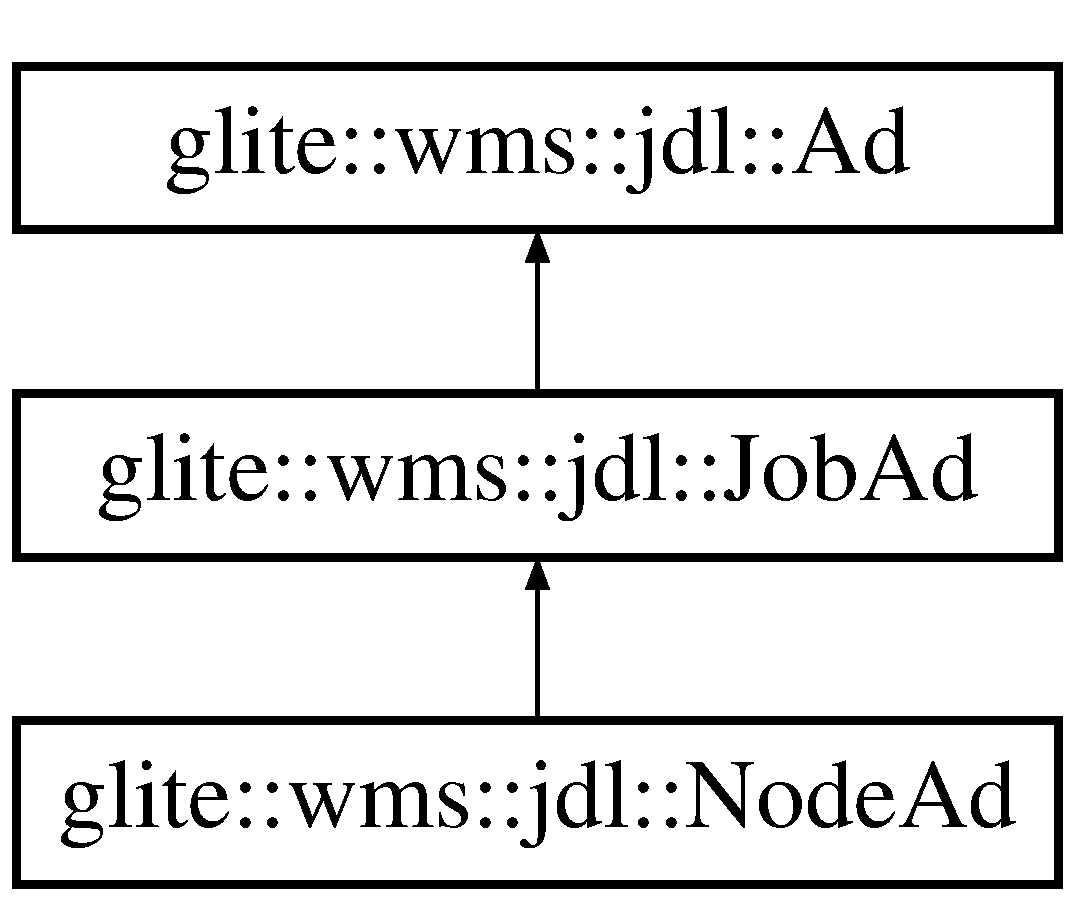
\includegraphics[height=3cm]{classglite_1_1wms_1_1jdl_1_1JobAd}
\end{center}
\end{figure}
\subsection*{Public Member Functions}
\begin{Indent}{\bf Constructors/Destructor}\par
\begin{CompactItemize}
\item 
\hyperlink{classglite_1_1wms_1_1jdl_1_1JobAd_z1_0}{Job\-Ad} ()
\item 
virtual \hyperlink{classglite_1_1wms_1_1jdl_1_1JobAd_z1_1}{$\sim$Job\-Ad} ()  throw ()
\item 
\hyperlink{classglite_1_1wms_1_1jdl_1_1JobAd_z1_2}{Job\-Ad} (const std::string \&jdl\_\-string)
\item 
\hyperlink{classglite_1_1wms_1_1jdl_1_1JobAd_z1_3}{Job\-Ad} (const classad::Class\-Ad \&class\-Ad)
\item 
\hyperlink{classglite_1_1wms_1_1jdl_1_1JobAd_z1_4}{Job\-Ad::Job\-Ad} (const \hyperlink{classglite_1_1wms_1_1jdl_1_1JobAd}{Job\-Ad} \&jobad)
\item 
void \hyperlink{classglite_1_1wms_1_1jdl_1_1JobAd_z1_5}{Job\-Ad::operator=} (const \hyperlink{classglite_1_1wms_1_1jdl_1_1JobAd}{Job\-Ad} \&jobad)
\end{CompactItemize}
\end{Indent}
\begin{Indent}{\bf String and Stream Constructor/Destructor}\par
\begin{CompactItemize}
\item 
void \hyperlink{classglite_1_1wms_1_1jdl_1_1JobAd_z3_0}{from\-Stream} (std::istream \&jdl\_\-in)
\item 
std::string \hyperlink{classglite_1_1wms_1_1jdl_1_1JobAd_z3_1}{to\-String} ()
\item 
std::string \hyperlink{classglite_1_1wms_1_1jdl_1_1JobAd_z3_2}{to\-String} (const std::string \&attr\_\-value)
\item 
std::string \hyperlink{classglite_1_1wms_1_1jdl_1_1JobAd_z3_3}{to\-Submission\-String} ()
\item 
void \hyperlink{classglite_1_1wms_1_1jdl_1_1JobAd_z3_4}{to\-File} (const std::string \&file\_\-path)
\end{CompactItemize}
\end{Indent}
\begin{Indent}{\bf Insertion Methods}\par
\begin{CompactItemize}
\item 
void \hyperlink{classglite_1_1wms_1_1jdl_1_1JobAd_z5_0}{set\-Default\-Rank} (const std::string \&attr\_\-value)
\item 
void \hyperlink{classglite_1_1wms_1_1jdl_1_1JobAd_z5_1}{set\-Default\-Req} (const std::string \&attr\_\-value)
\item 
void \hyperlink{classglite_1_1wms_1_1jdl_1_1JobAd_z5_2}{set\-Allowed\-Protocols} (const std::vector$<$ std::string $>$ \&attr\_\-value)
\item 
const std::vector$<$ std::string $>$ \hyperlink{classglite_1_1wms_1_1jdl_1_1JobAd_z5_3}{get\-Allowed\-Protocols} ()
\item 
void \hyperlink{classglite_1_1wms_1_1jdl_1_1JobAd_z5_4}{set\-Attribute\-Expr} (const std::string \&attr\_\-name, const std::string \&attr\_\-value)
\item 
void \hyperlink{classglite_1_1wms_1_1jdl_1_1JobAd_z5_5}{set\-Attribute\-Expr} (const std::string \&attr\_\-name, Expr\-Tree $\ast$attr\_\-value)
\end{CompactItemize}
\end{Indent}
\begin{Indent}{\bf Retrieval Methods}\par
\begin{CompactItemize}
\item 
\hyperlink{classglite_1_1wms_1_1jdl_1_1Ad}{Ad} \hyperlink{classglite_1_1wms_1_1jdl_1_1JobAd_z7_0}{get\-Ad} (const std::string \&attr\_\-name)
\item 
std::string \hyperlink{classglite_1_1wms_1_1jdl_1_1JobAd_z7_1}{get\-String} (const std::string \&attr\_\-name)
\item 
int \hyperlink{classglite_1_1wms_1_1jdl_1_1JobAd_z7_2}{get\-Int} (const std::string \&attr\_\-name)
\item 
double \hyperlink{classglite_1_1wms_1_1jdl_1_1JobAd_z7_3}{get\-Double} (const std::string \&attr\_\-name)
\item 
bool \hyperlink{classglite_1_1wms_1_1jdl_1_1JobAd_z7_4}{get\-Bool} (const std::string \&attr\_\-name)
\end{CompactItemize}
\end{Indent}
\begin{Indent}{\bf Miscellaneous Methods}\par
\begin{CompactItemize}
\item 
void \hyperlink{classglite_1_1wms_1_1jdl_1_1JobAd_z9_0}{check\-Syntax} (const std::string \&attr\_\-name, classad::Expr\-Tree $\ast$attr\_\-value)
\item 
void \hyperlink{classglite_1_1wms_1_1jdl_1_1JobAd_z9_1}{check\-Multi\-Attribute} (const std::vector$<$ std::string $>$ \&multi)
\item 
classad::Expr\-Tree $\ast$ \hyperlink{classglite_1_1wms_1_1jdl_1_1JobAd_z9_2}{del\-Attribute} (const std::string \&attr\_\-name)
\item 
void \hyperlink{classglite_1_1wms_1_1jdl_1_1JobAd_z9_3}{check} ()
\end{CompactItemize}
\end{Indent}
\subsection*{Protected Member Functions}
\begin{CompactItemize}
\item 
virtual void \hyperlink{classglite_1_1wms_1_1jdl_1_1JobAd_b0}{check\-Input\-Sandbox} (std::vector$<$ std::string $>$ \&extracted)
\item 
virtual void \hyperlink{classglite_1_1wms_1_1jdl_1_1JobAd_b1}{check\-Rank\-Req} ()
\item 
virtual void \hyperlink{classglite_1_1wms_1_1jdl_1_1JobAd_b2}{insert\-Attribute} (const std::string \&attr\_\-name, classad::Expr\-Tree $\ast$val)
\item 
std::vector$<$ std::string $>$ \hyperlink{classglite_1_1wms_1_1jdl_1_1JobAd_b3}{extract\-Files} (const std::string \&attr\_\-name, const std::string \&path, std::vector$<$ std::string $>$ \&extracted)
\end{CompactItemize}
\subsection*{Protected Attributes}
\begin{CompactItemize}
\item 
classad::Class\-Ad \hyperlink{classglite_1_1wms_1_1jdl_1_1JobAd_p0}{user}
\end{CompactItemize}
\subsection*{Friends}
\begin{CompactItemize}
\item 
class \hyperlink{classglite_1_1wms_1_1jdl_1_1JobAd_n0}{Job}
\item 
class \hyperlink{classglite_1_1wms_1_1jdl_1_1JobAd_n1}{Exp\-Dag\-Ad}
\end{CompactItemize}


\subsection{Detailed Description}
Provides a representation of the job description in the JDL language. 

Provides a representation of the job description in the JDL language and the functions for building and manipulating it. Basically the JDL is the Condor Class\-Ad language, so it is legitimate the direct use of the Condor API library for creating, modifying, deleting a job description. However the \hyperlink{classglite_1_1wms_1_1jdl_1_1JobAd}{Job\-Ad} class extends the Class\-Ad class of the Condor Class\-Ad library additionally providing some helper methods that ease the construction of job descriptions being fully compliant to WP1 WMS specification.

\begin{Desc}
\item[Version:]0.1 \end{Desc}
\begin{Desc}
\item[Date:]15 April 2002 \end{Desc}
\begin{Desc}
\item[Author:]Alessandro Maraschini $<$\href{mailto:alessandro.maraschini@datamat.it}{\tt alessandro.maraschini@datamat.it}$>$ \end{Desc}




\subsection{Constructor \& Destructor Documentation}
\hypertarget{classglite_1_1wms_1_1jdl_1_1JobAd_z1_0}{
\index{glite::wms::jdl::JobAd@{glite::wms::jdl::Job\-Ad}!JobAd@{JobAd}}
\index{JobAd@{JobAd}!glite::wms::jdl::JobAd@{glite::wms::jdl::Job\-Ad}}
\subsubsection[JobAd]{\setlength{\rightskip}{0pt plus 5cm}glite::wms::jdl::Job\-Ad::Job\-Ad ()}}
\label{classglite_1_1wms_1_1jdl_1_1JobAd_z1_0}


Instantiates an empty \hyperlink{classglite_1_1wms_1_1jdl_1_1JobAd}{Job\-Ad} object \hypertarget{classglite_1_1wms_1_1jdl_1_1JobAd_z1_1}{
\index{glite::wms::jdl::JobAd@{glite::wms::jdl::Job\-Ad}!~JobAd@{$\sim$JobAd}}
\index{~JobAd@{$\sim$JobAd}!glite::wms::jdl::JobAd@{glite::wms::jdl::Job\-Ad}}
\subsubsection[$\sim$JobAd]{\setlength{\rightskip}{0pt plus 5cm}virtual glite::wms::jdl::Job\-Ad::$\sim$\hyperlink{classglite_1_1wms_1_1jdl_1_1JobAd}{Job\-Ad} ()  throw ()\hspace{0.3cm}{\tt  \mbox{[}virtual\mbox{]}}}}
\label{classglite_1_1wms_1_1jdl_1_1JobAd_z1_1}


\hyperlink{classglite_1_1wms_1_1jdl_1_1JobAd}{Job\-Ad} destructor \hypertarget{classglite_1_1wms_1_1jdl_1_1JobAd_z1_2}{
\index{glite::wms::jdl::JobAd@{glite::wms::jdl::Job\-Ad}!JobAd@{JobAd}}
\index{JobAd@{JobAd}!glite::wms::jdl::JobAd@{glite::wms::jdl::Job\-Ad}}
\subsubsection[JobAd]{\setlength{\rightskip}{0pt plus 5cm}glite::wms::jdl::Job\-Ad::Job\-Ad (const std::string \& {\em jdl\_\-string})}}
\label{classglite_1_1wms_1_1jdl_1_1JobAd_z1_2}


Instantiates a \hyperlink{classglite_1_1wms_1_1jdl_1_1JobAd}{Job\-Ad} object from the given Class\-Ad-jdl string \begin{Desc}
\item[Parameters:]
\begin{description}
\item[{\em jdl\_\-string}]A string representig the description of the job \end{description}
\end{Desc}
\begin{Desc}
\item[Exceptions:]
\begin{description}
\item[{\em Ad\-Mismatch\-Exception}]- A value is not of the right type for an attribute name in the \hyperlink{classglite_1_1wms_1_1jdl_1_1JobAd}{Job\-Ad} \item[{\em Ad\-Format\-Exception}]A value is not in the right format for the an attribute name in the \hyperlink{classglite_1_1wms_1_1jdl_1_1JobAd}{Job\-Ad} \item[{\em Ad\-Syntax\-Exception}]Syntax error catched while trying to add an attribute \item[{\em Ad\-Class\-Ad\-Exception}]a class\-Ad method raised an error \item[{\em Ad\-List\-Exception}]A list has been mad with a non-list value attribute \end{description}
\end{Desc}
\hypertarget{classglite_1_1wms_1_1jdl_1_1JobAd_z1_3}{
\index{glite::wms::jdl::JobAd@{glite::wms::jdl::Job\-Ad}!JobAd@{JobAd}}
\index{JobAd@{JobAd}!glite::wms::jdl::JobAd@{glite::wms::jdl::Job\-Ad}}
\subsubsection[JobAd]{\setlength{\rightskip}{0pt plus 5cm}glite::wms::jdl::Job\-Ad::Job\-Ad (const classad::Class\-Ad \& {\em class\-Ad})}}
\label{classglite_1_1wms_1_1jdl_1_1JobAd_z1_3}


Constructor with a Class\-Ad instance \begin{Desc}
\item[Parameters:]
\begin{description}
\item[{\em class\-Ad}]the Class\-Ad instance where to build the \hyperlink{classglite_1_1wms_1_1jdl_1_1JobAd}{Job\-Ad} from\end{description}
\end{Desc}


\subsection{Member Function Documentation}
\hypertarget{classglite_1_1wms_1_1jdl_1_1JobAd_z9_3}{
\index{glite::wms::jdl::JobAd@{glite::wms::jdl::Job\-Ad}!check@{check}}
\index{check@{check}!glite::wms::jdl::JobAd@{glite::wms::jdl::Job\-Ad}}
\subsubsection[check]{\setlength{\rightskip}{0pt plus 5cm}void glite::wms::jdl::Job\-Ad::check ()}}
\label{classglite_1_1wms_1_1jdl_1_1JobAd_z9_3}


Check the \hyperlink{classglite_1_1wms_1_1jdl_1_1JobAd}{Job\-Ad} instance for both syntax and semanthic errors \begin{Desc}
\item[Exceptions:]
\begin{description}
\item[{\em Ad\-Mismatch\-Exception}]A value is not of the right type for an attribute name in the \hyperlink{classglite_1_1wms_1_1jdl_1_1JobAd}{Job\-Ad} \item[{\em Ad\-Format\-Exception}]A value is not in the right format for the an attribute name in the \hyperlink{classglite_1_1wms_1_1jdl_1_1JobAd}{Job\-Ad} \item[{\em Ad\-Syntax\-Exception}]Syntax error catched while trying to add an attribute \item[{\em Ad\-Class\-Ad\-Exception}]a class\-Ad method raised an error \item[{\em Ad\-List\-Exception}]A list has been mad with a non-list value attribute\end{description}
\end{Desc}
\hypertarget{classglite_1_1wms_1_1jdl_1_1JobAd_b0}{
\index{glite::wms::jdl::JobAd@{glite::wms::jdl::Job\-Ad}!checkInputSandbox@{checkInputSandbox}}
\index{checkInputSandbox@{checkInputSandbox}!glite::wms::jdl::JobAd@{glite::wms::jdl::Job\-Ad}}
\subsubsection[checkInputSandbox]{\setlength{\rightskip}{0pt plus 5cm}virtual void glite::wms::jdl::Job\-Ad::check\-Input\-Sandbox (std::vector$<$ std::string $>$ \& {\em extracted})\hspace{0.3cm}{\tt  \mbox{[}protected, virtual\mbox{]}}}}
\label{classglite_1_1wms_1_1jdl_1_1JobAd_b0}




Reimplemented in \hyperlink{classglite_1_1wms_1_1jdl_1_1NodeAd_b0}{glite::wms::jdl::Node\-Ad}.\hypertarget{classglite_1_1wms_1_1jdl_1_1JobAd_z9_1}{
\index{glite::wms::jdl::JobAd@{glite::wms::jdl::Job\-Ad}!checkMultiAttribute@{checkMultiAttribute}}
\index{checkMultiAttribute@{checkMultiAttribute}!glite::wms::jdl::JobAd@{glite::wms::jdl::Job\-Ad}}
\subsubsection[checkMultiAttribute]{\setlength{\rightskip}{0pt plus 5cm}void glite::wms::jdl::Job\-Ad::check\-Multi\-Attribute (const std::vector$<$ std::string $>$ \& {\em multi})}}
\label{classglite_1_1wms_1_1jdl_1_1JobAd_z9_1}


Check if the Member/is\-Member expression is properly used in rank and requirements attributes expressions \begin{Desc}
\item[Parameters:]
\begin{description}
\item[{\em multi}]a vector containing all the attributes that could be of multiple value type \end{description}
\end{Desc}
\begin{Desc}
\item[Exceptions:]
\begin{description}
\item[{\em Ad\-Syntax\-Exception}]when the Member/Is\-Member expression is badly used \end{description}
\end{Desc}
\hypertarget{classglite_1_1wms_1_1jdl_1_1JobAd_b1}{
\index{glite::wms::jdl::JobAd@{glite::wms::jdl::Job\-Ad}!checkRankReq@{checkRankReq}}
\index{checkRankReq@{checkRankReq}!glite::wms::jdl::JobAd@{glite::wms::jdl::Job\-Ad}}
\subsubsection[checkRankReq]{\setlength{\rightskip}{0pt plus 5cm}virtual void glite::wms::jdl::Job\-Ad::check\-Rank\-Req ()\hspace{0.3cm}{\tt  \mbox{[}protected, virtual\mbox{]}}}}
\label{classglite_1_1wms_1_1jdl_1_1JobAd_b1}


\hypertarget{classglite_1_1wms_1_1jdl_1_1JobAd_z9_0}{
\index{glite::wms::jdl::JobAd@{glite::wms::jdl::Job\-Ad}!checkSyntax@{checkSyntax}}
\index{checkSyntax@{checkSyntax}!glite::wms::jdl::JobAd@{glite::wms::jdl::Job\-Ad}}
\subsubsection[checkSyntax]{\setlength{\rightskip}{0pt plus 5cm}void glite::wms::jdl::Job\-Ad::check\-Syntax (const std::string \& {\em attr\_\-name}, classad::Expr\-Tree $\ast$ {\em attr\_\-value})}}
\label{classglite_1_1wms_1_1jdl_1_1JobAd_z9_0}


Check if the couple attribute/value is admitted \begin{Desc}
\item[Parameters:]
\begin{description}
\item[{\em attr\_\-name}]the name of the attribute \item[{\em attr\_\-value}]a pointer to an Expr\-Tree representing the value to be checkted \end{description}
\end{Desc}
\begin{Desc}
\item[Exceptions:]
\begin{description}
\item[{\em Ad\-Mismatch\-Exception}]The type of value is not allowed for the specified attribute name \end{description}
\end{Desc}
\hypertarget{classglite_1_1wms_1_1jdl_1_1JobAd_z9_2}{
\index{glite::wms::jdl::JobAd@{glite::wms::jdl::Job\-Ad}!delAttribute@{delAttribute}}
\index{delAttribute@{delAttribute}!glite::wms::jdl::JobAd@{glite::wms::jdl::Job\-Ad}}
\subsubsection[delAttribute]{\setlength{\rightskip}{0pt plus 5cm}classad::Expr\-Tree$\ast$ glite::wms::jdl::Job\-Ad::del\-Attribute (const std::string \& {\em attr\_\-name})\hspace{0.3cm}{\tt  \mbox{[}virtual\mbox{]}}}}
\label{classglite_1_1wms_1_1jdl_1_1JobAd_z9_2}


Delete an Attribute. It fails if the attribute doesn't exist \begin{Desc}
\item[Parameters:]
\begin{description}
\item[{\em attr\_\-nam}]The name of the attibute to be deleted \end{description}
\end{Desc}
\begin{Desc}
\item[Exceptions:]
\begin{description}
\item[{\em Ad\-Empty\-Exception}]The attribute has not been set yet \end{description}
\end{Desc}


Reimplemented from \hyperlink{classglite_1_1wms_1_1jdl_1_1Ad_z17_1}{glite::wms::jdl::Ad}.\hypertarget{classglite_1_1wms_1_1jdl_1_1JobAd_b3}{
\index{glite::wms::jdl::JobAd@{glite::wms::jdl::Job\-Ad}!extractFiles@{extractFiles}}
\index{extractFiles@{extractFiles}!glite::wms::jdl::JobAd@{glite::wms::jdl::Job\-Ad}}
\subsubsection[extractFiles]{\setlength{\rightskip}{0pt plus 5cm}std::vector$<$std::string$>$ glite::wms::jdl::Job\-Ad::extract\-Files (const std::string \& {\em attr\_\-name}, const std::string \& {\em path}, std::vector$<$ std::string $>$ \& {\em extracted})\hspace{0.3cm}{\tt  \mbox{[}protected\mbox{]}}}}
\label{classglite_1_1wms_1_1jdl_1_1JobAd_b3}


Analise a path and resolve the wildcards (if present) on it check the existence of (at least one file) the path. Leave URI/URL address unchanged \hypertarget{classglite_1_1wms_1_1jdl_1_1JobAd_z3_0}{
\index{glite::wms::jdl::JobAd@{glite::wms::jdl::Job\-Ad}!fromStream@{fromStream}}
\index{fromStream@{fromStream}!glite::wms::jdl::JobAd@{glite::wms::jdl::Job\-Ad}}
\subsubsection[fromStream]{\setlength{\rightskip}{0pt plus 5cm}void glite::wms::jdl::Job\-Ad::from\-Stream (std::istream \& {\em jdl\_\-in})}}
\label{classglite_1_1wms_1_1jdl_1_1JobAd_z3_0}


Update the \hyperlink{classglite_1_1wms_1_1jdl_1_1JobAd}{Job\-Ad} object with the given input stream. \begin{Desc}
\item[Parameters:]
\begin{description}
\item[{\em jdl\_\-in}]this is the job description passed in the form of a generic input stream so that it can be taken from a terminal input stream, file input stream, string streams etc. \end{description}
\end{Desc}
\begin{Desc}
\item[Exceptions:]
\begin{description}
\item[{\em Ad\-Mismatch\-Exception}]A value is not of the right type for an attribute name in the \hyperlink{classglite_1_1wms_1_1jdl_1_1JobAd}{Job\-Ad} \item[{\em Ad\-Format\-Exception}]A value is not in the right format for the an attribute name in the \hyperlink{classglite_1_1wms_1_1jdl_1_1JobAd}{Job\-Ad} \item[{\em Ad\-Syntax\-Exception}]Syntax error catched while trying to add an attribute \item[{\em Ad\-Class\-Ad\-Exception}]a class\-Ad method raised an error \item[{\em Ad\-List\-Exception}]A list has been mad with a non-list value attribute \end{description}
\end{Desc}
\hypertarget{classglite_1_1wms_1_1jdl_1_1JobAd_z7_0}{
\index{glite::wms::jdl::JobAd@{glite::wms::jdl::Job\-Ad}!getAd@{getAd}}
\index{getAd@{getAd}!glite::wms::jdl::JobAd@{glite::wms::jdl::Job\-Ad}}
\subsubsection[getAd]{\setlength{\rightskip}{0pt plus 5cm}\hyperlink{classglite_1_1wms_1_1jdl_1_1Ad}{Ad} glite::wms::jdl::Job\-Ad::get\-Ad (const std::string \& {\em attr\_\-name})}}
\label{classglite_1_1wms_1_1jdl_1_1JobAd_z7_0}


Retreive the value of the specified attribute \begin{Desc}
\item[Parameters:]
\begin{description}
\item[{\em attr\_\-name}]The name of the attribute name to be retrieved \end{description}
\end{Desc}
\begin{Desc}
\item[Returns:]the string representng the value of the specified attribute \end{Desc}
\begin{Desc}
\item[Exceptions:]
\begin{description}
\item[{\em Ad\-Empty\-Exception}]The checked attribute has not been set yet \item[{\em Ad\-Mismatch\-Exception}]The type of retrieved value is not allowed for the specified attribute name \end{description}
\end{Desc}
\hypertarget{classglite_1_1wms_1_1jdl_1_1JobAd_z5_3}{
\index{glite::wms::jdl::JobAd@{glite::wms::jdl::Job\-Ad}!getAllowedProtocols@{getAllowedProtocols}}
\index{getAllowedProtocols@{getAllowedProtocols}!glite::wms::jdl::JobAd@{glite::wms::jdl::Job\-Ad}}
\subsubsection[getAllowedProtocols]{\setlength{\rightskip}{0pt plus 5cm}const std::vector$<$std::string$>$ glite::wms::jdl::Job\-Ad::get\-Allowed\-Protocols ()}}
\label{classglite_1_1wms_1_1jdl_1_1JobAd_z5_3}


Retrieve the list of all allowed protocols for inputsandbox URL format \begin{Desc}
\item[Returns:]a vector containing all the protocols valid for the inputsandbox if provided with a URL format\end{Desc}
\hypertarget{classglite_1_1wms_1_1jdl_1_1JobAd_z7_4}{
\index{glite::wms::jdl::JobAd@{glite::wms::jdl::Job\-Ad}!getBool@{getBool}}
\index{getBool@{getBool}!glite::wms::jdl::JobAd@{glite::wms::jdl::Job\-Ad}}
\subsubsection[getBool]{\setlength{\rightskip}{0pt plus 5cm}bool glite::wms::jdl::Job\-Ad::get\-Bool (const std::string \& {\em attr\_\-name})}}
\label{classglite_1_1wms_1_1jdl_1_1JobAd_z7_4}


Retreive the value of the specified attribute \begin{Desc}
\item[Parameters:]
\begin{description}
\item[{\em attr\_\-name}]The name of the attribute name to be retrieved \end{description}
\end{Desc}
\begin{Desc}
\item[Returns:]the value of the specified attribute \end{Desc}
\begin{Desc}
\item[Exceptions:]
\begin{description}
\item[{\em Ad\-Empty\-Exception}]The checked attribute has not been set yet \item[{\em Ad\-Mismatch\-Exception}]The type of retrieved value is not allowed for the specified attribute name \end{description}
\end{Desc}
\hypertarget{classglite_1_1wms_1_1jdl_1_1JobAd_z7_3}{
\index{glite::wms::jdl::JobAd@{glite::wms::jdl::Job\-Ad}!getDouble@{getDouble}}
\index{getDouble@{getDouble}!glite::wms::jdl::JobAd@{glite::wms::jdl::Job\-Ad}}
\subsubsection[getDouble]{\setlength{\rightskip}{0pt plus 5cm}double glite::wms::jdl::Job\-Ad::get\-Double (const std::string \& {\em attr\_\-name})}}
\label{classglite_1_1wms_1_1jdl_1_1JobAd_z7_3}


Retreive the value of the specified attribute \begin{Desc}
\item[Parameters:]
\begin{description}
\item[{\em attr\_\-name}]The name of the attribute name to be retrieved \end{description}
\end{Desc}
\begin{Desc}
\item[Returns:]the value of the specified attribute \end{Desc}
\begin{Desc}
\item[Exceptions:]
\begin{description}
\item[{\em Ad\-Empty\-Exception}]The checked attribute has not been set yet \item[{\em Ad\-Mismatch\-Exception}]The type of retrieved value is not allowed for the specified attribute name \end{description}
\end{Desc}
\hypertarget{classglite_1_1wms_1_1jdl_1_1JobAd_z7_2}{
\index{glite::wms::jdl::JobAd@{glite::wms::jdl::Job\-Ad}!getInt@{getInt}}
\index{getInt@{getInt}!glite::wms::jdl::JobAd@{glite::wms::jdl::Job\-Ad}}
\subsubsection[getInt]{\setlength{\rightskip}{0pt plus 5cm}int glite::wms::jdl::Job\-Ad::get\-Int (const std::string \& {\em attr\_\-name})}}
\label{classglite_1_1wms_1_1jdl_1_1JobAd_z7_2}


Retreive the value of the specified attribute \begin{Desc}
\item[Parameters:]
\begin{description}
\item[{\em attr\_\-name}]The name of the attribute name to be retrieved \end{description}
\end{Desc}
\begin{Desc}
\item[Returns:]the value of the specified attribute \end{Desc}
\begin{Desc}
\item[Exceptions:]
\begin{description}
\item[{\em Ad\-Empty\-Exception}]The checked attribute has not been set yet \item[{\em Ad\-Mismatch\-Exception}]The type of retrieved value is not allowed for the specified attribute name \end{description}
\end{Desc}
\hypertarget{classglite_1_1wms_1_1jdl_1_1JobAd_z7_1}{
\index{glite::wms::jdl::JobAd@{glite::wms::jdl::Job\-Ad}!getString@{getString}}
\index{getString@{getString}!glite::wms::jdl::JobAd@{glite::wms::jdl::Job\-Ad}}
\subsubsection[getString]{\setlength{\rightskip}{0pt plus 5cm}std::string glite::wms::jdl::Job\-Ad::get\-String (const std::string \& {\em attr\_\-name})}}
\label{classglite_1_1wms_1_1jdl_1_1JobAd_z7_1}


Retreive the value of the specified attribute \begin{Desc}
\item[Parameters:]
\begin{description}
\item[{\em attr\_\-name}]The name of the attribute name to be retrieved \end{description}
\end{Desc}
\begin{Desc}
\item[Returns:]the value of the specified attribute \end{Desc}
\begin{Desc}
\item[Exceptions:]
\begin{description}
\item[{\em Ad\-Empty\-Exception}]The checked attribute has not been set yet \item[{\em Ad\-Mismatch\-Exception}]The type of retrieved value is not allowed for the specified attribute name \end{description}
\end{Desc}
\hypertarget{classglite_1_1wms_1_1jdl_1_1JobAd_b2}{
\index{glite::wms::jdl::JobAd@{glite::wms::jdl::Job\-Ad}!insertAttribute@{insertAttribute}}
\index{insertAttribute@{insertAttribute}!glite::wms::jdl::JobAd@{glite::wms::jdl::Job\-Ad}}
\subsubsection[insertAttribute]{\setlength{\rightskip}{0pt plus 5cm}virtual void glite::wms::jdl::Job\-Ad::insert\-Attribute (const std::string \& {\em attr\_\-name}, classad::Expr\-Tree $\ast$ {\em val})\hspace{0.3cm}{\tt  \mbox{[}protected, virtual\mbox{]}}}}
\label{classglite_1_1wms_1_1jdl_1_1JobAd_b2}


Insert a classad Exptression inside the \hyperlink{classglite_1_1wms_1_1jdl_1_1Ad}{Ad} instance \begin{Desc}
\item[Parameters:]
\begin{description}
\item[{\em attr\_\-name}]a string representing the attribute name \item[{\em val}]- The value of the attribute to be added\end{description}
\end{Desc}


Reimplemented from \hyperlink{classglite_1_1wms_1_1jdl_1_1Ad_b2}{glite::wms::jdl::Ad}.

Reimplemented in \hyperlink{classglite_1_1wms_1_1jdl_1_1NodeAd_b2}{glite::wms::jdl::Node\-Ad}.\hypertarget{classglite_1_1wms_1_1jdl_1_1JobAd_z1_4}{
\index{glite::wms::jdl::JobAd@{glite::wms::jdl::Job\-Ad}!JobAd::JobAd@{JobAd::JobAd}}
\index{JobAd::JobAd@{JobAd::JobAd}!glite::wms::jdl::JobAd@{glite::wms::jdl::Job\-Ad}}
\subsubsection[JobAd::JobAd]{\setlength{\rightskip}{0pt plus 5cm}glite::wms::jdl::Job\-Ad::Job\-Ad::Job\-Ad (const \hyperlink{classglite_1_1wms_1_1jdl_1_1JobAd}{Job\-Ad} \& {\em jobad})}}
\label{classglite_1_1wms_1_1jdl_1_1JobAd_z1_4}


Copy constructor \begin{Desc}
\item[Parameters:]
\begin{description}
\item[{\em jobad}]a \hyperlink{classglite_1_1wms_1_1jdl_1_1JobAd}{Job\-Ad} instance to be copied \end{description}
\end{Desc}
\hypertarget{classglite_1_1wms_1_1jdl_1_1JobAd_z1_5}{
\index{glite::wms::jdl::JobAd@{glite::wms::jdl::Job\-Ad}!JobAd::operator=@{JobAd::operator=}}
\index{JobAd::operator=@{JobAd::operator=}!glite::wms::jdl::JobAd@{glite::wms::jdl::Job\-Ad}}
\subsubsection[JobAd::operator=]{\setlength{\rightskip}{0pt plus 5cm}void glite::wms::jdl::Job\-Ad::Job\-Ad::operator= (const \hyperlink{classglite_1_1wms_1_1jdl_1_1JobAd}{Job\-Ad} \& {\em jobad})}}
\label{classglite_1_1wms_1_1jdl_1_1JobAd_z1_5}


Operator $\ast$ \hypertarget{classglite_1_1wms_1_1jdl_1_1JobAd_z5_2}{
\index{glite::wms::jdl::JobAd@{glite::wms::jdl::Job\-Ad}!setAllowedProtocols@{setAllowedProtocols}}
\index{setAllowedProtocols@{setAllowedProtocols}!glite::wms::jdl::JobAd@{glite::wms::jdl::Job\-Ad}}
\subsubsection[setAllowedProtocols]{\setlength{\rightskip}{0pt plus 5cm}void glite::wms::jdl::Job\-Ad::set\-Allowed\-Protocols (const std::vector$<$ std::string $>$ \& {\em attr\_\-value})}}
\label{classglite_1_1wms_1_1jdl_1_1JobAd_z5_2}


Add a list of protocols to the set of allowed inputsandbox protocols \begin{Desc}
\item[Parameters:]
\begin{description}
\item[{\em attr\_\-value}]the list of protocol to be allowed for inputsandbox URL values\end{description}
\end{Desc}
\hypertarget{classglite_1_1wms_1_1jdl_1_1JobAd_z5_5}{
\index{glite::wms::jdl::JobAd@{glite::wms::jdl::Job\-Ad}!setAttributeExpr@{setAttributeExpr}}
\index{setAttributeExpr@{setAttributeExpr}!glite::wms::jdl::JobAd@{glite::wms::jdl::Job\-Ad}}
\subsubsection[setAttributeExpr]{\setlength{\rightskip}{0pt plus 5cm}void glite::wms::jdl::Job\-Ad::set\-Attribute\-Expr (const std::string \& {\em attr\_\-name}, Expr\-Tree $\ast$ {\em attr\_\-value})\hspace{0.3cm}{\tt  \mbox{[}virtual\mbox{]}}}}
\label{classglite_1_1wms_1_1jdl_1_1JobAd_z5_5}


Add The specified Expression Attribute to the jdl istance \begin{Desc}
\item[Parameters:]
\begin{description}
\item[{\em attr\_\-name}]The Name of the attribute to be added \item[{\em attr\_\-value}]The string expression of the attribute to be added \end{description}
\end{Desc}
\begin{Desc}
\item[Exceptions:]
\begin{description}
\item[{\em Ad\-Mismatch\-Exception}]The type of value is not allowed for the specified attribute name \item[{\em Ad\-Class\-Ad\-Exception}]a class\-Ad method raised an error \end{description}
\end{Desc}


Reimplemented from \hyperlink{classglite_1_1wms_1_1jdl_1_1Ad_z19_15}{glite::wms::jdl::Ad}.\hypertarget{classglite_1_1wms_1_1jdl_1_1JobAd_z5_4}{
\index{glite::wms::jdl::JobAd@{glite::wms::jdl::Job\-Ad}!setAttributeExpr@{setAttributeExpr}}
\index{setAttributeExpr@{setAttributeExpr}!glite::wms::jdl::JobAd@{glite::wms::jdl::Job\-Ad}}
\subsubsection[setAttributeExpr]{\setlength{\rightskip}{0pt plus 5cm}void glite::wms::jdl::Job\-Ad::set\-Attribute\-Expr (const std::string \& {\em attr\_\-name}, const std::string \& {\em attr\_\-value})\hspace{0.3cm}{\tt  \mbox{[}virtual\mbox{]}}}}
\label{classglite_1_1wms_1_1jdl_1_1JobAd_z5_4}


Add The specified Expression Attribute to the jdl istance \begin{Desc}
\item[Parameters:]
\begin{description}
\item[{\em attr\_\-name}]The Name of the attribute to be added \item[{\em attr\_\-value}]The string expression of the attribute to be added \end{description}
\end{Desc}
\begin{Desc}
\item[Exceptions:]
\begin{description}
\item[{\em Ad\-Mismatch\-Exception}]The type of value is not allowed for the specified attribute name \item[{\em Ad\-Class\-Ad\-Exception}]a class\-Ad method raised an error \end{description}
\end{Desc}


Reimplemented from \hyperlink{classglite_1_1wms_1_1jdl_1_1Ad_z19_8}{glite::wms::jdl::Ad}.\hypertarget{classglite_1_1wms_1_1jdl_1_1JobAd_z5_0}{
\index{glite::wms::jdl::JobAd@{glite::wms::jdl::Job\-Ad}!setDefaultRank@{setDefaultRank}}
\index{setDefaultRank@{setDefaultRank}!glite::wms::jdl::JobAd@{glite::wms::jdl::Job\-Ad}}
\subsubsection[setDefaultRank]{\setlength{\rightskip}{0pt plus 5cm}void glite::wms::jdl::Job\-Ad::set\-Default\-Rank (const std::string \& {\em attr\_\-value})}}
\label{classglite_1_1wms_1_1jdl_1_1JobAd_z5_0}


Set the default value for Rank attribute (take in consideration if not specified in JDL) \begin{Desc}
\item[Parameters:]
\begin{description}
\item[{\em attr\_\-value}]the value to be set to the default rank\end{description}
\end{Desc}
\hypertarget{classglite_1_1wms_1_1jdl_1_1JobAd_z5_1}{
\index{glite::wms::jdl::JobAd@{glite::wms::jdl::Job\-Ad}!setDefaultReq@{setDefaultReq}}
\index{setDefaultReq@{setDefaultReq}!glite::wms::jdl::JobAd@{glite::wms::jdl::Job\-Ad}}
\subsubsection[setDefaultReq]{\setlength{\rightskip}{0pt plus 5cm}void glite::wms::jdl::Job\-Ad::set\-Default\-Req (const std::string \& {\em attr\_\-value})}}
\label{classglite_1_1wms_1_1jdl_1_1JobAd_z5_1}


Set the default value for Requirements attribute (take in consideration if not specified in JDL) \begin{Desc}
\item[Parameters:]
\begin{description}
\item[{\em attr\_\-value}]the value to be set to the default requirements\end{description}
\end{Desc}
\hypertarget{classglite_1_1wms_1_1jdl_1_1JobAd_z3_4}{
\index{glite::wms::jdl::JobAd@{glite::wms::jdl::Job\-Ad}!toFile@{toFile}}
\index{toFile@{toFile}!glite::wms::jdl::JobAd@{glite::wms::jdl::Job\-Ad}}
\subsubsection[toFile]{\setlength{\rightskip}{0pt plus 5cm}void glite::wms::jdl::Job\-Ad::to\-File (const std::string \& {\em file\_\-path})}}
\label{classglite_1_1wms_1_1jdl_1_1JobAd_z3_4}


Put the \hyperlink{classglite_1_1wms_1_1jdl_1_1JobAd}{Job\-Ad} Instance as a string into a file \begin{Desc}
\item[Parameters:]
\begin{description}
\item[{\em file\_\-path}]the string representation of the file where to copy the \hyperlink{classglite_1_1wms_1_1jdl_1_1JobAd}{Job\-Ad} to\end{description}
\end{Desc}
\hypertarget{classglite_1_1wms_1_1jdl_1_1JobAd_z3_2}{
\index{glite::wms::jdl::JobAd@{glite::wms::jdl::Job\-Ad}!toString@{toString}}
\index{toString@{toString}!glite::wms::jdl::JobAd@{glite::wms::jdl::Job\-Ad}}
\subsubsection[toString]{\setlength{\rightskip}{0pt plus 5cm}std::string glite::wms::jdl::Job\-Ad::to\-String (const std::string \& {\em attr\_\-value})\hspace{0.3cm}{\tt  \mbox{[}virtual\mbox{]}}}}
\label{classglite_1_1wms_1_1jdl_1_1JobAd_z3_2}


Convert an \hyperlink{classglite_1_1wms_1_1jdl_1_1Ad}{Ad} attribute into its string representation \begin{Desc}
\item[Parameters:]
\begin{description}
\item[{\em attr\_\-name}]the attribute to be looked up \end{description}
\end{Desc}
\begin{Desc}
\item[Returns:]return the attrbute string representation \end{Desc}


Reimplemented from \hyperlink{classglite_1_1wms_1_1jdl_1_1Ad_z15_1}{glite::wms::jdl::Ad}.\hypertarget{classglite_1_1wms_1_1jdl_1_1JobAd_z3_1}{
\index{glite::wms::jdl::JobAd@{glite::wms::jdl::Job\-Ad}!toString@{toString}}
\index{toString@{toString}!glite::wms::jdl::JobAd@{glite::wms::jdl::Job\-Ad}}
\subsubsection[toString]{\setlength{\rightskip}{0pt plus 5cm}std::string glite::wms::jdl::Job\-Ad::to\-String ()\hspace{0.3cm}{\tt  \mbox{[}virtual\mbox{]}}}}
\label{classglite_1_1wms_1_1jdl_1_1JobAd_z3_1}


Convert the \hyperlink{classglite_1_1wms_1_1jdl_1_1JobAd}{Job\-Ad} Instance into a single line string representation 

Reimplemented from \hyperlink{classglite_1_1wms_1_1jdl_1_1Ad_z15_0}{glite::wms::jdl::Ad}.\hypertarget{classglite_1_1wms_1_1jdl_1_1JobAd_z3_3}{
\index{glite::wms::jdl::JobAd@{glite::wms::jdl::Job\-Ad}!toSubmissionString@{toSubmissionString}}
\index{toSubmissionString@{toSubmissionString}!glite::wms::jdl::JobAd@{glite::wms::jdl::Job\-Ad}}
\subsubsection[toSubmissionString]{\setlength{\rightskip}{0pt plus 5cm}std::string glite::wms::jdl::Job\-Ad::to\-Submission\-String ()}}
\label{classglite_1_1wms_1_1jdl_1_1JobAd_z3_3}


Convert the \hyperlink{classglite_1_1wms_1_1jdl_1_1JobAd}{Job\-Ad} Instance into a single line string representation ready for submission \begin{Desc}
\item[Returns:]the string reoresentation that goes to the Network\-Server \end{Desc}


\subsection{Friends And Related Function Documentation}
\hypertarget{classglite_1_1wms_1_1jdl_1_1JobAd_n1}{
\index{glite::wms::jdl::JobAd@{glite::wms::jdl::Job\-Ad}!ExpDagAd@{ExpDagAd}}
\index{ExpDagAd@{ExpDagAd}!glite::wms::jdl::JobAd@{glite::wms::jdl::Job\-Ad}}
\subsubsection[ExpDagAd]{\setlength{\rightskip}{0pt plus 5cm}friend class \hyperlink{classglite_1_1wms_1_1jdl_1_1ExpDagAd}{Exp\-Dag\-Ad}\hspace{0.3cm}{\tt  \mbox{[}friend\mbox{]}}}}
\label{classglite_1_1wms_1_1jdl_1_1JobAd_n1}




Reimplemented in \hyperlink{classglite_1_1wms_1_1jdl_1_1NodeAd_n0}{glite::wms::jdl::Node\-Ad}.\hypertarget{classglite_1_1wms_1_1jdl_1_1JobAd_n0}{
\index{glite::wms::jdl::JobAd@{glite::wms::jdl::Job\-Ad}!Job@{Job}}
\index{Job@{Job}!glite::wms::jdl::JobAd@{glite::wms::jdl::Job\-Ad}}
\subsubsection[Job]{\setlength{\rightskip}{0pt plus 5cm}friend class Job\hspace{0.3cm}{\tt  \mbox{[}friend\mbox{]}}}}
\label{classglite_1_1wms_1_1jdl_1_1JobAd_n0}




\subsection{Member Data Documentation}
\hypertarget{classglite_1_1wms_1_1jdl_1_1JobAd_p0}{
\index{glite::wms::jdl::JobAd@{glite::wms::jdl::Job\-Ad}!user@{user}}
\index{user@{user}!glite::wms::jdl::JobAd@{glite::wms::jdl::Job\-Ad}}
\subsubsection[user]{\setlength{\rightskip}{0pt plus 5cm}classad::Class\-Ad \hyperlink{classglite_1_1wms_1_1jdl_1_1JobAd_p0}{glite::wms::jdl::Job\-Ad::user}\hspace{0.3cm}{\tt  \mbox{[}protected\mbox{]}}}}
\label{classglite_1_1wms_1_1jdl_1_1JobAd_p0}


user class\-Ad: calssad containing all the attributes that could be possibly changed by the check method. This member is utilized in order to ripristinate (restore method ) the old classad situation 

The documentation for this class was generated from the following file:\begin{CompactItemize}
\item 
\hyperlink{JobAd_8h}{Job\-Ad.h}\end{CompactItemize}

\hypertarget{classglite_1_1wms_1_1jdl_1_1JobAdSchema}{
\section{glite::wms::jdl::Job\-Ad\-Schema Class Reference}
\label{classglite_1_1wms_1_1jdl_1_1JobAdSchema}\index{glite::wms::jdl::JobAdSchema@{glite::wms::jdl::JobAdSchema}}
}
{\tt \#include $<$Job\-Ad\-Schema.h$>$}

\subsection*{Public Types}
\begin{CompactItemize}
\item 
enum \hyperlink{classglite_1_1wms_1_1jdl_1_1JobAdSchema_w6}{attribute} \{ \par
\hyperlink{classglite_1_1wms_1_1jdl_1_1JobAdSchema_w6w0}{SCHEMA\_\-DAC}, 
\hyperlink{classglite_1_1wms_1_1jdl_1_1JobAdSchema_w6w1}{SCHEMA\_\-RTE}, 
\hyperlink{classglite_1_1wms_1_1jdl_1_1JobAdSchema_w6w2}{SCHEMA\_\-TCPU}, 
\hyperlink{classglite_1_1wms_1_1jdl_1_1JobAdSchema_w6w3}{SCHEMA\_\-FCPU}, 
\par
\hyperlink{classglite_1_1wms_1_1jdl_1_1JobAdSchema_w6w4}{SCHEMA\_\-OIP}, 
\hyperlink{classglite_1_1wms_1_1jdl_1_1JobAdSchema_w6w5}{SCHEMA\_\-ARRAY}
 \}
\end{CompactItemize}
\subsection*{Public Member Functions}
\begin{CompactItemize}
\item 
\hyperlink{classglite_1_1wms_1_1jdl_1_1JobAdSchema_a0}{Job\-Ad\-Schema} (std::vector$<$ std::string $>$ values)
\item 
std::string \hyperlink{classglite_1_1wms_1_1jdl_1_1JobAdSchema_a1}{get} (\hyperlink{classglite_1_1wms_1_1jdl_1_1JobAdSchema_w6}{attribute} attr\-Name)
\item 
\hyperlink{classglite_1_1wms_1_1jdl_1_1JobAdSchema}{Job\-Ad\-Schema} $\ast$ \hyperlink{classglite_1_1wms_1_1jdl_1_1JobAdSchema_a2}{Copy} ()
\end{CompactItemize}
\subsection*{Static Public Member Functions}
\begin{CompactItemize}
\item 
\hyperlink{classglite_1_1wms_1_1jdl_1_1JobAdSchema}{Job\-Ad\-Schema} $\ast$ \hyperlink{classglite_1_1wms_1_1jdl_1_1JobAdSchema_e0}{glue\-Schema} ()
\item 
\hyperlink{classglite_1_1wms_1_1jdl_1_1JobAdSchema}{Job\-Ad\-Schema} \hyperlink{classglite_1_1wms_1_1jdl_1_1JobAdSchema_e1}{edg\-Schema} ()
\end{CompactItemize}


\subsection{Detailed Description}
Provides a Schema used to check the attribute in the \hyperlink{classglite_1_1wms_1_1jdl_1_1JobAd}{Job\-Ad} The default utilised schema is GLUE. To instanciate a schema you will need to provide an array of Strings, one per attribute \begin{Desc}
\item[Version:]0.1 \end{Desc}
\begin{Desc}
\item[Author:]Alessandro Maraschini $<$\href{mailto:alessandro.maraschini@datamat.it}{\tt alessandro.maraschini@datamat.it}$>$ \end{Desc}




\subsection{Member Enumeration Documentation}
\hypertarget{classglite_1_1wms_1_1jdl_1_1JobAdSchema_w6}{
\index{glite::wms::jdl::JobAdSchema@{glite::wms::jdl::Job\-Ad\-Schema}!attribute@{attribute}}
\index{attribute@{attribute}!glite::wms::jdl::JobAdSchema@{glite::wms::jdl::Job\-Ad\-Schema}}
\subsubsection[attribute]{\setlength{\rightskip}{0pt plus 5cm}enum \hyperlink{classglite_1_1wms_1_1jdl_1_1JobAdSchema_w6}{glite::wms::jdl::Job\-Ad\-Schema::attribute}}}
\label{classglite_1_1wms_1_1jdl_1_1JobAdSchema_w6}


\begin{Desc}
\item[Enumeration values: ]\par
\begin{description}
\index{SCHEMA_DAC@{SCHEMA\_\-DAC}!glite::wms::jdl::JobAdSchema@{glite::wms::jdl::JobAdSchema}}\index{glite::wms::jdl::JobAdSchema@{glite::wms::jdl::JobAdSchema}!SCHEMA_DAC@{SCHEMA\_\-DAC}}\item[{\em 
\hypertarget{classglite_1_1wms_1_1jdl_1_1JobAdSchema_w6w0}{
SCHEMA\_\-DAC}
\label{classglite_1_1wms_1_1jdl_1_1JobAdSchema_w6w0}
}]other.Data\-Access\-Cost attribute \index{SCHEMA_RTE@{SCHEMA\_\-RTE}!glite::wms::jdl::JobAdSchema@{glite::wms::jdl::JobAdSchema}}\index{glite::wms::jdl::JobAdSchema@{glite::wms::jdl::JobAdSchema}!SCHEMA_RTE@{SCHEMA\_\-RTE}}\item[{\em 
\hypertarget{classglite_1_1wms_1_1jdl_1_1JobAdSchema_w6w1}{
SCHEMA\_\-RTE}
\label{classglite_1_1wms_1_1jdl_1_1JobAdSchema_w6w1}
}]other.Glue\-Host\-Application\-Software\-Run\-Time\-Environment attribute. Appended for MPI jobs in Requirements expression \index{SCHEMA_TCPU@{SCHEMA\_\-TCPU}!glite::wms::jdl::JobAdSchema@{glite::wms::jdl::JobAdSchema}}\index{glite::wms::jdl::JobAdSchema@{glite::wms::jdl::JobAdSchema}!SCHEMA_TCPU@{SCHEMA\_\-TCPU}}\item[{\em 
\hypertarget{classglite_1_1wms_1_1jdl_1_1JobAdSchema_w6w2}{
SCHEMA\_\-TCPU}
\label{classglite_1_1wms_1_1jdl_1_1JobAdSchema_w6w2}
}]other.Glue\-CEInfo\-Total\-CPUs attribute. Appended for MPI jobs in Requirements expression \index{SCHEMA_FCPU@{SCHEMA\_\-FCPU}!glite::wms::jdl::JobAdSchema@{glite::wms::jdl::JobAdSchema}}\index{glite::wms::jdl::JobAdSchema@{glite::wms::jdl::JobAdSchema}!SCHEMA_FCPU@{SCHEMA\_\-FCPU}}\item[{\em 
\hypertarget{classglite_1_1wms_1_1jdl_1_1JobAdSchema_w6w3}{
SCHEMA\_\-FCPU}
\label{classglite_1_1wms_1_1jdl_1_1JobAdSchema_w6w3}
}]other.Glue\-CEState\-Free\-CPUs attribute Set for MPI jobs as a default rank (if not given) \index{SCHEMA_OIP@{SCHEMA\_\-OIP}!glite::wms::jdl::JobAdSchema@{glite::wms::jdl::JobAdSchema}}\index{glite::wms::jdl::JobAdSchema@{glite::wms::jdl::JobAdSchema}!SCHEMA_OIP@{SCHEMA\_\-OIP}}\item[{\em 
\hypertarget{classglite_1_1wms_1_1jdl_1_1JobAdSchema_w6w4}{
SCHEMA\_\-OIP}
\label{classglite_1_1wms_1_1jdl_1_1JobAdSchema_w6w4}
}]other.Glue\-Host\-Network\-Adapter\-Outbound\-IP Added for Interactive Jobs in requirements expression \index{SCHEMA_ARRAY@{SCHEMA\_\-ARRAY}!glite::wms::jdl::JobAdSchema@{glite::wms::jdl::JobAdSchema}}\index{glite::wms::jdl::JobAdSchema@{glite::wms::jdl::JobAdSchema}!SCHEMA_ARRAY@{SCHEMA\_\-ARRAY}}\item[{\em 
\hypertarget{classglite_1_1wms_1_1jdl_1_1JobAdSchema_w6w5}{
SCHEMA\_\-ARRAY}
\label{classglite_1_1wms_1_1jdl_1_1JobAdSchema_w6w5}
}]Max index array dimension for Schema Attributes \end{description}
\end{Desc}



\subsection{Constructor \& Destructor Documentation}
\hypertarget{classglite_1_1wms_1_1jdl_1_1JobAdSchema_a0}{
\index{glite::wms::jdl::JobAdSchema@{glite::wms::jdl::Job\-Ad\-Schema}!JobAdSchema@{JobAdSchema}}
\index{JobAdSchema@{JobAdSchema}!glite::wms::jdl::JobAdSchema@{glite::wms::jdl::Job\-Ad\-Schema}}
\subsubsection[JobAdSchema]{\setlength{\rightskip}{0pt plus 5cm}glite::wms::jdl::Job\-Ad\-Schema::Job\-Ad\-Schema (std::vector$<$ std::string $>$ {\em values})}}
\label{classglite_1_1wms_1_1jdl_1_1JobAdSchema_a0}


CUSTOM schema constructor \begin{Desc}
\item[Parameters:]
\begin{description}
\item[{\em values}]an array of string of \hyperlink{classglite_1_1wms_1_1jdl_1_1JobAdSchema_w6w5}{SCHEMA\_\-ARRAY} dimension \end{description}
\end{Desc}


\subsection{Member Function Documentation}
\hypertarget{classglite_1_1wms_1_1jdl_1_1JobAdSchema_a2}{
\index{glite::wms::jdl::JobAdSchema@{glite::wms::jdl::Job\-Ad\-Schema}!Copy@{Copy}}
\index{Copy@{Copy}!glite::wms::jdl::JobAdSchema@{glite::wms::jdl::Job\-Ad\-Schema}}
\subsubsection[Copy]{\setlength{\rightskip}{0pt plus 5cm}\hyperlink{classglite_1_1wms_1_1jdl_1_1JobAdSchema}{Job\-Ad\-Schema}$\ast$ glite::wms::jdl::Job\-Ad\-Schema::Copy ()}}
\label{classglite_1_1wms_1_1jdl_1_1JobAdSchema_a2}


Make a deep copy of the current \hyperlink{classglite_1_1wms_1_1jdl_1_1JobAdSchema}{Job\-Ad\-Schema} instance \begin{Desc}
\item[Returns:]the copy of the current schema \end{Desc}
\hypertarget{classglite_1_1wms_1_1jdl_1_1JobAdSchema_e1}{
\index{glite::wms::jdl::JobAdSchema@{glite::wms::jdl::Job\-Ad\-Schema}!edgSchema@{edgSchema}}
\index{edgSchema@{edgSchema}!glite::wms::jdl::JobAdSchema@{glite::wms::jdl::Job\-Ad\-Schema}}
\subsubsection[edgSchema]{\setlength{\rightskip}{0pt plus 5cm}\hyperlink{classglite_1_1wms_1_1jdl_1_1JobAdSchema}{Job\-Ad\-Schema} glite::wms::jdl::Job\-Ad\-Schema::edg\-Schema ()\hspace{0.3cm}{\tt  \mbox{[}static\mbox{]}}}}
\label{classglite_1_1wms_1_1jdl_1_1JobAdSchema_e1}


EDG schema static constructor: deprecated \hypertarget{classglite_1_1wms_1_1jdl_1_1JobAdSchema_a1}{
\index{glite::wms::jdl::JobAdSchema@{glite::wms::jdl::Job\-Ad\-Schema}!get@{get}}
\index{get@{get}!glite::wms::jdl::JobAdSchema@{glite::wms::jdl::Job\-Ad\-Schema}}
\subsubsection[get]{\setlength{\rightskip}{0pt plus 5cm}std::string glite::wms::jdl::Job\-Ad\-Schema::get (\hyperlink{classglite_1_1wms_1_1jdl_1_1JobAdSchema_w6}{attribute} {\em attr\-Name})}}
\label{classglite_1_1wms_1_1jdl_1_1JobAdSchema_a1}


Retrieve the value for a specified attribute  the attribute to be retrieved \begin{Desc}
\item[Returns:]the string representation of the value to be retrieved \end{Desc}
\hypertarget{classglite_1_1wms_1_1jdl_1_1JobAdSchema_e0}{
\index{glite::wms::jdl::JobAdSchema@{glite::wms::jdl::Job\-Ad\-Schema}!glueSchema@{glueSchema}}
\index{glueSchema@{glueSchema}!glite::wms::jdl::JobAdSchema@{glite::wms::jdl::Job\-Ad\-Schema}}
\subsubsection[glueSchema]{\setlength{\rightskip}{0pt plus 5cm}\hyperlink{classglite_1_1wms_1_1jdl_1_1JobAdSchema}{Job\-Ad\-Schema}$\ast$ glite::wms::jdl::Job\-Ad\-Schema::glue\-Schema ()\hspace{0.3cm}{\tt  \mbox{[}static\mbox{]}}}}
\label{classglite_1_1wms_1_1jdl_1_1JobAdSchema_e0}


GLUE schema static constructor (\hyperlink{classglite_1_1wms_1_1jdl_1_1JobAd}{Job\-Ad} default utilised schema) 

The documentation for this class was generated from the following file:\begin{CompactItemize}
\item 
\hyperlink{JobAdSchema_8h}{Job\-Ad\-Schema.h}\end{CompactItemize}

\hypertarget{structglite_1_1wms_1_1jdl_1_1JobIdStruct}{
\section{glite::wms::jdl::Job\-Id\-Struct Struct Reference}
\label{structglite_1_1wms_1_1jdl_1_1JobIdStruct}\index{glite::wms::jdl::JobIdStruct@{glite::wms::jdl::JobIdStruct}}
}
{\tt \#include $<$Exp\-Dag\-Ad.h$>$}

\subsection*{Public Attributes}
\begin{CompactItemize}
\item 
glite::wmsutils::jobid::Job\-Id \hyperlink{structglite_1_1wms_1_1jdl_1_1JobIdStruct_o0}{jobid}
\item 
std::string $\ast$ \hyperlink{structglite_1_1wms_1_1jdl_1_1JobIdStruct_o1}{node\-Name}
\item 
std::vector$<$ \hyperlink{structglite_1_1wms_1_1jdl_1_1JobIdStruct}{Job\-Id\-Struct} $\ast$ $>$ \hyperlink{structglite_1_1wms_1_1jdl_1_1JobIdStruct_o2}{children}
\end{CompactItemize}


\subsection{Detailed Description}
Used to specify the Job\-Id of a Dag and of all its nodes recoursively (each node could be a Dag itself) name can be NULL 



\subsection{Member Data Documentation}
\hypertarget{structglite_1_1wms_1_1jdl_1_1JobIdStruct_o2}{
\index{glite::wms::jdl::JobIdStruct@{glite::wms::jdl::Job\-Id\-Struct}!children@{children}}
\index{children@{children}!glite::wms::jdl::JobIdStruct@{glite::wms::jdl::Job\-Id\-Struct}}
\subsubsection[children]{\setlength{\rightskip}{0pt plus 5cm}std::vector$<$ \hyperlink{structglite_1_1wms_1_1jdl_1_1JobIdStruct}{Job\-Id\-Struct}$\ast$ $>$ \hyperlink{structglite_1_1wms_1_1jdl_1_1JobIdStruct_o2}{glite::wms::jdl::Job\-Id\-Struct::children}}}
\label{structglite_1_1wms_1_1jdl_1_1JobIdStruct_o2}


The list of the sub-jobs of this struct (0-size vector if of job type) \hypertarget{structglite_1_1wms_1_1jdl_1_1JobIdStruct_o0}{
\index{glite::wms::jdl::JobIdStruct@{glite::wms::jdl::Job\-Id\-Struct}!jobid@{jobid}}
\index{jobid@{jobid}!glite::wms::jdl::JobIdStruct@{glite::wms::jdl::Job\-Id\-Struct}}
\subsubsection[jobid]{\setlength{\rightskip}{0pt plus 5cm}glite::wmsutils::jobid::Job\-Id \hyperlink{structglite_1_1wms_1_1jdl_1_1JobIdStruct_o0}{glite::wms::jdl::Job\-Id\-Struct::jobid}}}
\label{structglite_1_1wms_1_1jdl_1_1JobIdStruct_o0}


The identifier of the job \hypertarget{structglite_1_1wms_1_1jdl_1_1JobIdStruct_o1}{
\index{glite::wms::jdl::JobIdStruct@{glite::wms::jdl::Job\-Id\-Struct}!nodeName@{nodeName}}
\index{nodeName@{nodeName}!glite::wms::jdl::JobIdStruct@{glite::wms::jdl::Job\-Id\-Struct}}
\subsubsection[nodeName]{\setlength{\rightskip}{0pt plus 5cm}std::string$\ast$ \hyperlink{structglite_1_1wms_1_1jdl_1_1JobIdStruct_o1}{glite::wms::jdl::Job\-Id\-Struct::node\-Name}}}
\label{structglite_1_1wms_1_1jdl_1_1JobIdStruct_o1}


The name of the node 

The documentation for this struct was generated from the following file:\begin{CompactItemize}
\item 
\hyperlink{ExpDagAd_8h}{Exp\-Dag\-Ad.h}\end{CompactItemize}

\hypertarget{classglite_1_1wms_1_1jdl_1_1ManipulationException}{
\section{glite::wms::jdl::Manipulation\-Exception Class Reference}
\label{classglite_1_1wms_1_1jdl_1_1ManipulationException}\index{glite::wms::jdl::ManipulationException@{glite::wms::jdl::ManipulationException}}
}
{\tt \#include $<$Manipulation\-Exceptions.h$>$}

Inheritance diagram for glite::wms::jdl::Manipulation\-Exception::\begin{figure}[H]
\begin{center}
\leavevmode
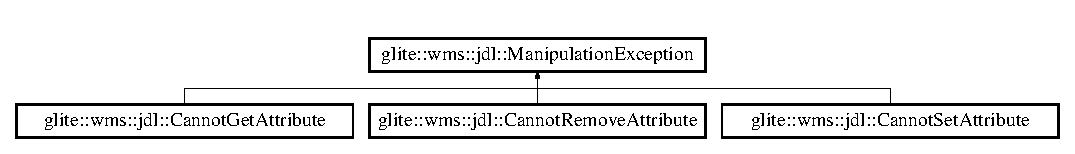
\includegraphics[height=1.62319cm]{classglite_1_1wms_1_1jdl_1_1ManipulationException}
\end{center}
\end{figure}
\subsection*{Public Member Functions}
\begin{CompactItemize}
\item 
\hyperlink{classglite_1_1wms_1_1jdl_1_1ManipulationException_a0}{Manipulation\-Exception} (const std::string \&parameter)
\item 
virtual \hyperlink{classglite_1_1wms_1_1jdl_1_1ManipulationException_a1}{$\sim$Manipulation\-Exception} (void)  throw ()
\item 
std::string \hyperlink{classglite_1_1wms_1_1jdl_1_1ManipulationException_a2}{parameter} (void) const 
\item 
virtual const char $\ast$ \hyperlink{classglite_1_1wms_1_1jdl_1_1ManipulationException_a3}{what} (void) const   throw ()
\item 
virtual std::string \hyperlink{classglite_1_1wms_1_1jdl_1_1ManipulationException_a4}{reason} (void) const 
\end{CompactItemize}
\subsection*{Protected Attributes}
\begin{CompactItemize}
\item 
std::string \hyperlink{classglite_1_1wms_1_1jdl_1_1ManipulationException_p0}{me\_\-parameter}
\end{CompactItemize}


\subsection{Constructor \& Destructor Documentation}
\hypertarget{classglite_1_1wms_1_1jdl_1_1ManipulationException_a0}{
\index{glite::wms::jdl::ManipulationException@{glite::wms::jdl::Manipulation\-Exception}!ManipulationException@{ManipulationException}}
\index{ManipulationException@{ManipulationException}!glite::wms::jdl::ManipulationException@{glite::wms::jdl::Manipulation\-Exception}}
\subsubsection[ManipulationException]{\setlength{\rightskip}{0pt plus 5cm}glite::wms::jdl::Manipulation\-Exception::Manipulation\-Exception (const std::string \& {\em parameter})\hspace{0.3cm}{\tt  \mbox{[}explicit\mbox{]}}}}
\label{classglite_1_1wms_1_1jdl_1_1ManipulationException_a0}


\hypertarget{classglite_1_1wms_1_1jdl_1_1ManipulationException_a1}{
\index{glite::wms::jdl::ManipulationException@{glite::wms::jdl::Manipulation\-Exception}!~ManipulationException@{$\sim$ManipulationException}}
\index{~ManipulationException@{$\sim$ManipulationException}!glite::wms::jdl::ManipulationException@{glite::wms::jdl::Manipulation\-Exception}}
\subsubsection[$\sim$ManipulationException]{\setlength{\rightskip}{0pt plus 5cm}virtual glite::wms::jdl::Manipulation\-Exception::$\sim$\hyperlink{classglite_1_1wms_1_1jdl_1_1ManipulationException}{Manipulation\-Exception} (void)  throw ()\hspace{0.3cm}{\tt  \mbox{[}virtual\mbox{]}}}}
\label{classglite_1_1wms_1_1jdl_1_1ManipulationException_a1}




\subsection{Member Function Documentation}
\hypertarget{classglite_1_1wms_1_1jdl_1_1ManipulationException_a2}{
\index{glite::wms::jdl::ManipulationException@{glite::wms::jdl::Manipulation\-Exception}!parameter@{parameter}}
\index{parameter@{parameter}!glite::wms::jdl::ManipulationException@{glite::wms::jdl::Manipulation\-Exception}}
\subsubsection[parameter]{\setlength{\rightskip}{0pt plus 5cm}std::string glite::wms::jdl::Manipulation\-Exception::parameter (void) const\hspace{0.3cm}{\tt  \mbox{[}inline\mbox{]}}}}
\label{classglite_1_1wms_1_1jdl_1_1ManipulationException_a2}


\hypertarget{classglite_1_1wms_1_1jdl_1_1ManipulationException_a4}{
\index{glite::wms::jdl::ManipulationException@{glite::wms::jdl::Manipulation\-Exception}!reason@{reason}}
\index{reason@{reason}!glite::wms::jdl::ManipulationException@{glite::wms::jdl::Manipulation\-Exception}}
\subsubsection[reason]{\setlength{\rightskip}{0pt plus 5cm}virtual std::string glite::wms::jdl::Manipulation\-Exception::reason (void) const\hspace{0.3cm}{\tt  \mbox{[}virtual\mbox{]}}}}
\label{classglite_1_1wms_1_1jdl_1_1ManipulationException_a4}




Reimplemented in \hyperlink{classglite_1_1wms_1_1jdl_1_1CannotGetAttribute_a2}{glite::wms::jdl::Cannot\-Get\-Attribute}, \hyperlink{classglite_1_1wms_1_1jdl_1_1CannotSetAttribute_a2}{glite::wms::jdl::Cannot\-Set\-Attribute}, and \hyperlink{classglite_1_1wms_1_1jdl_1_1CannotRemoveAttribute_a2}{glite::wms::jdl::Cannot\-Remove\-Attribute}.\hypertarget{classglite_1_1wms_1_1jdl_1_1ManipulationException_a3}{
\index{glite::wms::jdl::ManipulationException@{glite::wms::jdl::Manipulation\-Exception}!what@{what}}
\index{what@{what}!glite::wms::jdl::ManipulationException@{glite::wms::jdl::Manipulation\-Exception}}
\subsubsection[what]{\setlength{\rightskip}{0pt plus 5cm}virtual const char$\ast$ glite::wms::jdl::Manipulation\-Exception::what (void) const  throw ()\hspace{0.3cm}{\tt  \mbox{[}virtual\mbox{]}}}}
\label{classglite_1_1wms_1_1jdl_1_1ManipulationException_a3}




\subsection{Member Data Documentation}
\hypertarget{classglite_1_1wms_1_1jdl_1_1ManipulationException_p0}{
\index{glite::wms::jdl::ManipulationException@{glite::wms::jdl::Manipulation\-Exception}!me_parameter@{me\_\-parameter}}
\index{me_parameter@{me\_\-parameter}!glite::wms::jdl::ManipulationException@{glite::wms::jdl::Manipulation\-Exception}}
\subsubsection[me\_\-parameter]{\setlength{\rightskip}{0pt plus 5cm}std::string \hyperlink{classglite_1_1wms_1_1jdl_1_1ManipulationException_p0}{glite::wms::jdl::Manipulation\-Exception::me\_\-parameter}\hspace{0.3cm}{\tt  \mbox{[}protected\mbox{]}}}}
\label{classglite_1_1wms_1_1jdl_1_1ManipulationException_p0}




The documentation for this class was generated from the following file:\begin{CompactItemize}
\item 
\hyperlink{ManipulationExceptions_8h}{Manipulation\-Exceptions.h}\end{CompactItemize}

\hypertarget{classglite_1_1wms_1_1jdl_1_1NodeAd}{
\section{glite::wms::jdl::Node\-Ad Class Reference}
\label{classglite_1_1wms_1_1jdl_1_1NodeAd}\index{glite::wms::jdl::NodeAd@{glite::wms::jdl::NodeAd}}
}
Provides a representation of the job description in the JDL language.  


{\tt \#include $<$Node\-Ad.h$>$}

Inheritance diagram for glite::wms::jdl::Node\-Ad::\begin{figure}[H]
\begin{center}
\leavevmode
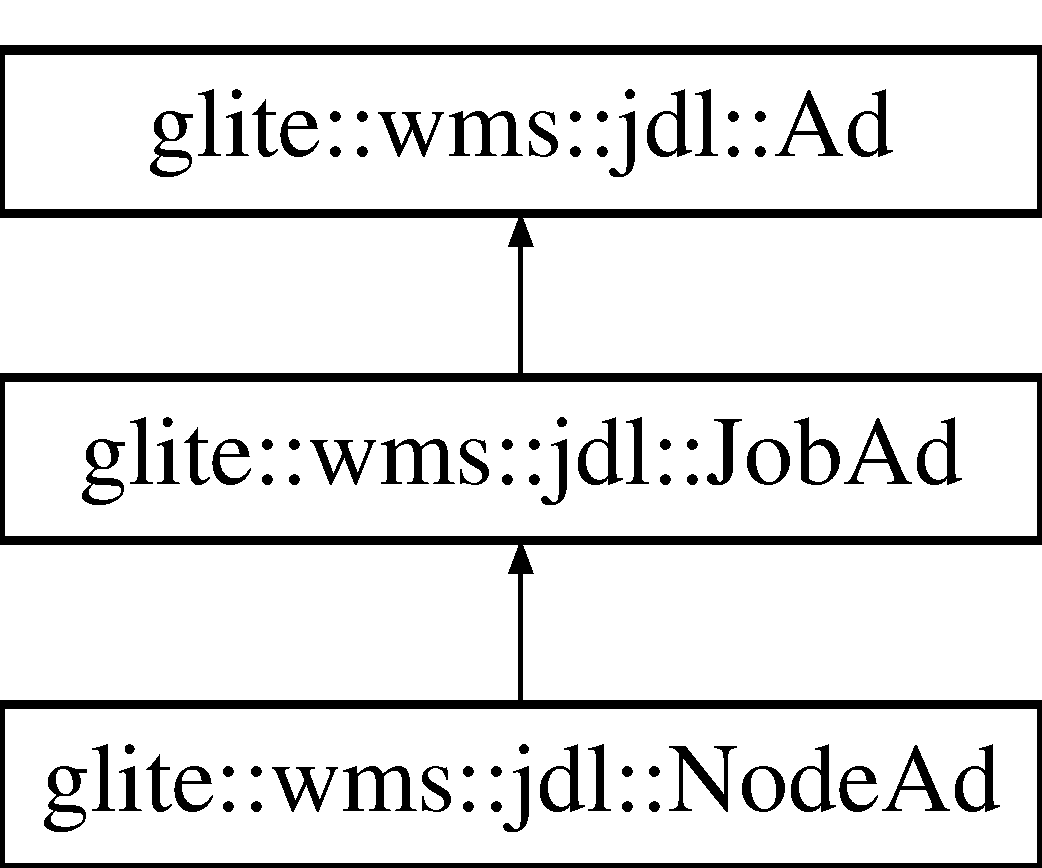
\includegraphics[height=3cm]{classglite_1_1wms_1_1jdl_1_1NodeAd}
\end{center}
\end{figure}
\subsection*{Public Member Functions}
\begin{CompactItemize}
\item 
\hyperlink{classglite_1_1wms_1_1jdl_1_1NodeAd_a0}{Node\-Ad} (const classad::Class\-Ad \&class\-Ad)
\item 
\hyperlink{classglite_1_1wms_1_1jdl_1_1NodeAd_a1}{Node\-Ad} ()
\item 
virtual \hyperlink{classglite_1_1wms_1_1jdl_1_1NodeAd_a2}{$\sim$Node\-Ad} ()  throw ()
\item 
std::vector$<$ classad::Expr\-Tree $\ast$ $>$ \hyperlink{classglite_1_1wms_1_1jdl_1_1NodeAd_a3}{get\-Remote\-Sandbox} ()
\item 
void \hyperlink{classglite_1_1wms_1_1jdl_1_1NodeAd_a4}{add\-User\-Tag} (const std::string \&attr\_\-name, const std::string \&attr\_\-value)
\end{CompactItemize}
\subsection*{Protected Member Functions}
\begin{CompactItemize}
\item 
void \hyperlink{classglite_1_1wms_1_1jdl_1_1NodeAd_b0}{check\-Input\-Sandbox} (std::vector$<$ std::string $>$ \&extracted)
\item 
void \hyperlink{classglite_1_1wms_1_1jdl_1_1NodeAd_b1}{check\-Specials} ()
\item 
void \hyperlink{classglite_1_1wms_1_1jdl_1_1NodeAd_b2}{insert\-Attribute} (const std::string \&attr\_\-name, classad::Expr\-Tree $\ast$val)
\end{CompactItemize}
\subsection*{Friends}
\begin{CompactItemize}
\item 
class \hyperlink{classglite_1_1wms_1_1jdl_1_1NodeAd_n0}{Exp\-Dag\-Ad}
\end{CompactItemize}


\subsection{Detailed Description}
Provides a representation of the job description in the JDL language. 

\begin{Desc}
\item[Version:]0.1 \end{Desc}
\begin{Desc}
\item[Date:]15 April 2002 \end{Desc}
\begin{Desc}
\item[Author:]Alessandro Maraschini $<$\href{mailto:alessandro.maraschini@datamat.it}{\tt alessandro.maraschini@datamat.it}$>$ \end{Desc}




\subsection{Constructor \& Destructor Documentation}
\hypertarget{classglite_1_1wms_1_1jdl_1_1NodeAd_a0}{
\index{glite::wms::jdl::NodeAd@{glite::wms::jdl::Node\-Ad}!NodeAd@{NodeAd}}
\index{NodeAd@{NodeAd}!glite::wms::jdl::NodeAd@{glite::wms::jdl::Node\-Ad}}
\subsubsection[NodeAd]{\setlength{\rightskip}{0pt plus 5cm}glite::wms::jdl::Node\-Ad::Node\-Ad (const classad::Class\-Ad \& {\em class\-Ad})\hspace{0.3cm}{\tt  \mbox{[}inline\mbox{]}}}}
\label{classglite_1_1wms_1_1jdl_1_1NodeAd_a0}


Constructory by Classad\hypertarget{classglite_1_1wms_1_1jdl_1_1NodeAd_a1}{
\index{glite::wms::jdl::NodeAd@{glite::wms::jdl::Node\-Ad}!NodeAd@{NodeAd}}
\index{NodeAd@{NodeAd}!glite::wms::jdl::NodeAd@{glite::wms::jdl::Node\-Ad}}
\subsubsection[NodeAd]{\setlength{\rightskip}{0pt plus 5cm}glite::wms::jdl::Node\-Ad::Node\-Ad ()\hspace{0.3cm}{\tt  \mbox{[}inline\mbox{]}}}}
\label{classglite_1_1wms_1_1jdl_1_1NodeAd_a1}


Default constructor\hypertarget{classglite_1_1wms_1_1jdl_1_1NodeAd_a2}{
\index{glite::wms::jdl::NodeAd@{glite::wms::jdl::Node\-Ad}!~NodeAd@{$\sim$NodeAd}}
\index{~NodeAd@{$\sim$NodeAd}!glite::wms::jdl::NodeAd@{glite::wms::jdl::Node\-Ad}}
\subsubsection[$\sim$NodeAd]{\setlength{\rightskip}{0pt plus 5cm}virtual glite::wms::jdl::Node\-Ad::$\sim$\hyperlink{classglite_1_1wms_1_1jdl_1_1NodeAd}{Node\-Ad} ()  throw ()\hspace{0.3cm}{\tt  \mbox{[}virtual\mbox{]}}}}
\label{classglite_1_1wms_1_1jdl_1_1NodeAd_a2}


Default Destructor 

\subsection{Member Function Documentation}
\hypertarget{classglite_1_1wms_1_1jdl_1_1NodeAd_a4}{
\index{glite::wms::jdl::NodeAd@{glite::wms::jdl::Node\-Ad}!addUserTag@{addUserTag}}
\index{addUserTag@{addUserTag}!glite::wms::jdl::NodeAd@{glite::wms::jdl::Node\-Ad}}
\subsubsection[addUserTag]{\setlength{\rightskip}{0pt plus 5cm}void glite::wms::jdl::Node\-Ad::add\-User\-Tag (const std::string \& {\em attr\_\-name}, const std::string \& {\em attr\_\-value})}}
\label{classglite_1_1wms_1_1jdl_1_1NodeAd_a4}


Add a User\-Tag to the node \begin{Desc}
\item[Parameters:]
\begin{description}
\item[{\em attr\_\-name}]the name of the usertag to be added \item[{\em attr\_\-value}]the value for the usertag\end{description}
\end{Desc}
\hypertarget{classglite_1_1wms_1_1jdl_1_1NodeAd_b0}{
\index{glite::wms::jdl::NodeAd@{glite::wms::jdl::Node\-Ad}!checkInputSandbox@{checkInputSandbox}}
\index{checkInputSandbox@{checkInputSandbox}!glite::wms::jdl::NodeAd@{glite::wms::jdl::Node\-Ad}}
\subsubsection[checkInputSandbox]{\setlength{\rightskip}{0pt plus 5cm}void glite::wms::jdl::Node\-Ad::check\-Input\-Sandbox (std::vector$<$ std::string $>$ \& {\em extracted})\hspace{0.3cm}{\tt  \mbox{[}protected, virtual\mbox{]}}}}
\label{classglite_1_1wms_1_1jdl_1_1NodeAd_b0}


Check Input\-Sandbox value. Could be overloaded in order to perform different checks \begin{Desc}
\item[Parameters:]
\begin{description}
\item[{\em extracted}]a vector listing all the files that have to be extracted i.e. whoose path has to be solved\end{description}
\end{Desc}


Reimplemented from \hyperlink{classglite_1_1wms_1_1jdl_1_1JobAd_b0}{glite::wms::jdl::Job\-Ad}.\hypertarget{classglite_1_1wms_1_1jdl_1_1NodeAd_b1}{
\index{glite::wms::jdl::NodeAd@{glite::wms::jdl::Node\-Ad}!checkSpecials@{checkSpecials}}
\index{checkSpecials@{checkSpecials}!glite::wms::jdl::NodeAd@{glite::wms::jdl::Node\-Ad}}
\subsubsection[checkSpecials]{\setlength{\rightskip}{0pt plus 5cm}void glite::wms::jdl::Node\-Ad::check\-Specials ()\hspace{0.3cm}{\tt  \mbox{[}protected, virtual\mbox{]}}}}
\label{classglite_1_1wms_1_1jdl_1_1NodeAd_b1}


Perform Special checks for Virtual\-Organisation attribute Notice: for a \hyperlink{classglite_1_1wms_1_1jdl_1_1NodeAd}{Node\-Ad} instance it is not mandatory (as for a \hyperlink{classglite_1_1wms_1_1jdl_1_1JobAd}{Job\-Ad}) 

Reimplemented from \hyperlink{classglite_1_1wms_1_1jdl_1_1JobAd}{glite::wms::jdl::Job\-Ad}.\hypertarget{classglite_1_1wms_1_1jdl_1_1NodeAd_a3}{
\index{glite::wms::jdl::NodeAd@{glite::wms::jdl::Node\-Ad}!getRemoteSandbox@{getRemoteSandbox}}
\index{getRemoteSandbox@{getRemoteSandbox}!glite::wms::jdl::NodeAd@{glite::wms::jdl::Node\-Ad}}
\subsubsection[getRemoteSandbox]{\setlength{\rightskip}{0pt plus 5cm}std::vector$<$classad::Expr\-Tree$\ast$$>$ glite::wms::jdl::Node\-Ad::get\-Remote\-Sandbox ()}}
\label{classglite_1_1wms_1_1jdl_1_1NodeAd_a3}


Retrieve the input\-Sandbox remote files extracted while checking the \hyperlink{classglite_1_1wms_1_1jdl_1_1Ad}{Ad} \begin{Desc}
\item[Returns:]a vector of all the Expression of remote sandbox i.e. all the \_\-$<$sbx file$>$ linked in the inputsandbox attribute\end{Desc}
\hypertarget{classglite_1_1wms_1_1jdl_1_1NodeAd_b2}{
\index{glite::wms::jdl::NodeAd@{glite::wms::jdl::Node\-Ad}!insertAttribute@{insertAttribute}}
\index{insertAttribute@{insertAttribute}!glite::wms::jdl::NodeAd@{glite::wms::jdl::Node\-Ad}}
\subsubsection[insertAttribute]{\setlength{\rightskip}{0pt plus 5cm}void glite::wms::jdl::Node\-Ad::insert\-Attribute (const std::string \& {\em attr\_\-name}, classad::Expr\-Tree $\ast$ {\em val})\hspace{0.3cm}{\tt  \mbox{[}protected, virtual\mbox{]}}}}
\label{classglite_1_1wms_1_1jdl_1_1NodeAd_b2}


\hyperlink{classglite_1_1wms_1_1jdl_1_1JobAd}{Job\-Ad} overloaded method: used to insert an attribute inside the classad \begin{Desc}
\item[Parameters:]
\begin{description}
\item[{\em attr\_\-name}]the name of the attribute \item[{\em val}]the value of the inserted attribute as a classad expression\end{description}
\end{Desc}


Reimplemented from \hyperlink{classglite_1_1wms_1_1jdl_1_1JobAd_b2}{glite::wms::jdl::Job\-Ad}.

\subsection{Friends And Related Function Documentation}
\hypertarget{classglite_1_1wms_1_1jdl_1_1NodeAd_n0}{
\index{glite::wms::jdl::NodeAd@{glite::wms::jdl::Node\-Ad}!ExpDagAd@{ExpDagAd}}
\index{ExpDagAd@{ExpDagAd}!glite::wms::jdl::NodeAd@{glite::wms::jdl::Node\-Ad}}
\subsubsection[ExpDagAd]{\setlength{\rightskip}{0pt plus 5cm}friend class \hyperlink{classglite_1_1wms_1_1jdl_1_1ExpDagAd}{Exp\-Dag\-Ad}\hspace{0.3cm}{\tt  \mbox{[}friend\mbox{]}}}}
\label{classglite_1_1wms_1_1jdl_1_1NodeAd_n0}




Reimplemented from \hyperlink{classglite_1_1wms_1_1jdl_1_1JobAd_n1}{glite::wms::jdl::Job\-Ad}.

The documentation for this class was generated from the following file:\begin{CompactItemize}
\item 
\hyperlink{NodeAd_8h}{Node\-Ad.h}\end{CompactItemize}

\hypertarget{structglite_1_1wms_1_1jdl_1_1NodeStruct}{
\section{glite::wms::jdl::Node\-Struct Struct Reference}
\label{structglite_1_1wms_1_1jdl_1_1NodeStruct}\index{glite::wms::jdl::NodeStruct@{glite::wms::jdl::NodeStruct}}
}
{\tt \#include $<$adconverter.h$>$}

\subsection*{Public Attributes}
\begin{CompactItemize}
\item 
std::string $\ast$ \hyperlink{structglite_1_1wms_1_1jdl_1_1NodeStruct_o0}{name}
\item 
std::vector$<$ \hyperlink{structglite_1_1wms_1_1jdl_1_1NodeStruct}{Node\-Struct} $\ast$ $>$ \hyperlink{structglite_1_1wms_1_1jdl_1_1NodeStruct_o1}{children\-Nodes}
\end{CompactItemize}


\subsection{Detailed Description}
Used to design the dependency structure among the nodes of a dag. Each node specifies its name and all the nodes that directly depend on it. when the name is NULL this structure does not represent an actual node, but it lists all the nodes that don't depend on any other node. 



\subsection{Member Data Documentation}
\hypertarget{structglite_1_1wms_1_1jdl_1_1NodeStruct_o1}{
\index{glite::wms::jdl::NodeStruct@{glite::wms::jdl::Node\-Struct}!childrenNodes@{childrenNodes}}
\index{childrenNodes@{childrenNodes}!glite::wms::jdl::NodeStruct@{glite::wms::jdl::Node\-Struct}}
\subsubsection[childrenNodes]{\setlength{\rightskip}{0pt plus 5cm}std::vector$<$ \hyperlink{structglite_1_1wms_1_1jdl_1_1NodeStruct}{Node\-Struct}$\ast$ $>$ \hyperlink{structglite_1_1wms_1_1jdl_1_1NodeStruct_o1}{glite::wms::jdl::Node\-Struct::children\-Nodes}}}
\label{structglite_1_1wms_1_1jdl_1_1NodeStruct_o1}


The list of all the node that depend on this node (0-size vector if empty) \hypertarget{structglite_1_1wms_1_1jdl_1_1NodeStruct_o0}{
\index{glite::wms::jdl::NodeStruct@{glite::wms::jdl::Node\-Struct}!name@{name}}
\index{name@{name}!glite::wms::jdl::NodeStruct@{glite::wms::jdl::Node\-Struct}}
\subsubsection[name]{\setlength{\rightskip}{0pt plus 5cm}std::string$\ast$ \hyperlink{structglite_1_1wms_1_1jdl_1_1NodeStruct_o0}{glite::wms::jdl::Node\-Struct::name}}}
\label{structglite_1_1wms_1_1jdl_1_1NodeStruct_o0}


The name of the node 

The documentation for this struct was generated from the following file:\begin{CompactItemize}
\item 
\hyperlink{adconverter_8h}{adconverter.h}\end{CompactItemize}

\hypertarget{classglite_1_1wms_1_1jdl_1_1RequestAdException}{
\section{glite::wms::jdl::Request\-Ad\-Exception Class Reference}
\label{classglite_1_1wms_1_1jdl_1_1RequestAdException}\index{glite::wms::jdl::RequestAdException@{glite::wms::jdl::RequestAdException}}
}
{\tt \#include $<$Request\-Ad\-Exceptions.h$>$}

Inheritance diagram for glite::wms::jdl::Request\-Ad\-Exception::\begin{figure}[H]
\begin{center}
\leavevmode
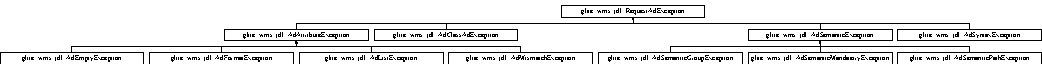
\includegraphics[height=0.854093cm]{classglite_1_1wms_1_1jdl_1_1RequestAdException}
\end{center}
\end{figure}
\subsection*{Public Member Functions}
\begin{CompactItemize}
\item 
std::string \hyperlink{classglite_1_1wms_1_1jdl_1_1RequestAdException_a0}{what} ()  throw ()
\end{CompactItemize}
\subsection*{Protected Member Functions}
\begin{CompactItemize}
\item 
\hyperlink{classglite_1_1wms_1_1jdl_1_1RequestAdException_b0}{Request\-Ad\-Exception} (std::string file, int line, std::string method, int code, std::string exception\_\-name)
\item 
virtual \hyperlink{classglite_1_1wms_1_1jdl_1_1RequestAdException_b1}{$\sim$Request\-Ad\-Exception} ()  throw ()
\end{CompactItemize}
\subsection*{Protected Attributes}
\begin{CompactItemize}
\item 
std::string \hyperlink{classglite_1_1wms_1_1jdl_1_1RequestAdException_p0}{error\_\-description}
\end{CompactItemize}


\subsection{Detailed Description}
\hyperlink{classglite_1_1wms_1_1jdl_1_1RequestAdException}{Request\-Ad\-Exception} This Exception is thrown when a bad usage of the \hyperlink{classglite_1_1wms_1_1jdl_1_1JobAd}{Job\-Ad} class is made \begin{Desc}
\item[Version:]0.1 \end{Desc}
\begin{Desc}
\item[Date:]15 April 2002 \end{Desc}
\begin{Desc}
\item[Author:]Alessandro Maraschini $<$\href{mailto:alessandro.maraschini@datamat.it}{\tt alessandro.maraschini@datamat.it}$>$ \end{Desc}




\subsection{Constructor \& Destructor Documentation}
\hypertarget{classglite_1_1wms_1_1jdl_1_1RequestAdException_b0}{
\index{glite::wms::jdl::RequestAdException@{glite::wms::jdl::Request\-Ad\-Exception}!RequestAdException@{RequestAdException}}
\index{RequestAdException@{RequestAdException}!glite::wms::jdl::RequestAdException@{glite::wms::jdl::Request\-Ad\-Exception}}
\subsubsection[RequestAdException]{\setlength{\rightskip}{0pt plus 5cm}glite::wms::jdl::Request\-Ad\-Exception::Request\-Ad\-Exception (std::string {\em file}, int {\em line}, std::string {\em method}, int {\em code}, std::string {\em exception\_\-name})\hspace{0.3cm}{\tt  \mbox{[}protected\mbox{]}}}}
\label{classglite_1_1wms_1_1jdl_1_1RequestAdException_b0}


Update all mandatory Exception Information \hypertarget{classglite_1_1wms_1_1jdl_1_1RequestAdException_b1}{
\index{glite::wms::jdl::RequestAdException@{glite::wms::jdl::Request\-Ad\-Exception}!~RequestAdException@{$\sim$RequestAdException}}
\index{~RequestAdException@{$\sim$RequestAdException}!glite::wms::jdl::RequestAdException@{glite::wms::jdl::Request\-Ad\-Exception}}
\subsubsection[$\sim$RequestAdException]{\setlength{\rightskip}{0pt plus 5cm}virtual glite::wms::jdl::Request\-Ad\-Exception::$\sim$\hyperlink{classglite_1_1wms_1_1jdl_1_1RequestAdException}{Request\-Ad\-Exception} ()  throw ()\hspace{0.3cm}{\tt  \mbox{[}inline, protected, virtual\mbox{]}}}}
\label{classglite_1_1wms_1_1jdl_1_1RequestAdException_b1}




\subsection{Member Function Documentation}
\hypertarget{classglite_1_1wms_1_1jdl_1_1RequestAdException_a0}{
\index{glite::wms::jdl::RequestAdException@{glite::wms::jdl::Request\-Ad\-Exception}!what@{what}}
\index{what@{what}!glite::wms::jdl::RequestAdException@{glite::wms::jdl::Request\-Ad\-Exception}}
\subsubsection[what]{\setlength{\rightskip}{0pt plus 5cm}std::string glite::wms::jdl::Request\-Ad\-Exception::what ()  throw ()}}
\label{classglite_1_1wms_1_1jdl_1_1RequestAdException_a0}




\subsection{Member Data Documentation}
\hypertarget{classglite_1_1wms_1_1jdl_1_1RequestAdException_p0}{
\index{glite::wms::jdl::RequestAdException@{glite::wms::jdl::Request\-Ad\-Exception}!error_description@{error\_\-description}}
\index{error_description@{error\_\-description}!glite::wms::jdl::RequestAdException@{glite::wms::jdl::Request\-Ad\-Exception}}
\subsubsection[error\_\-description]{\setlength{\rightskip}{0pt plus 5cm}std::string \hyperlink{classglite_1_1wms_1_1jdl_1_1RequestAdException_p0}{glite::wms::jdl::Request\-Ad\-Exception::error\_\-description}\hspace{0.3cm}{\tt  \mbox{[}protected\mbox{]}}}}
\label{classglite_1_1wms_1_1jdl_1_1RequestAdException_p0}




The documentation for this class was generated from the following file:\begin{CompactItemize}
\item 
\hyperlink{RequestAdExceptions_8h}{Request\-Ad\-Exceptions.h}\end{CompactItemize}


}

\subsection{Job Identifier API---C++ binding}
\label{jobidcpp}
{
\renewenvironment{CompactList}{\itemize\itemsep -2pt}{\enditemize}
\def\section#1{}
\renewcommand{\contentsline}[4]{{\bf #2}\leaders\hbox{.}\hfill #3}
The documentation of C$++$ Job Identifier API presented in this section was
generated automatically from the comments in the API header files by Doxygen.
The package providing the Job Identifier API is {\verb!org.glite.wms-utils.jobid!} for C$++$. The Java API is included
in package {\verb!org.glite.wms-ui.api-java!}

The class hierarchy is depicted in the following list.
\section{Glite Job\-Id API: CPP - Documentation Class Hierarchy}
This inheritance list is sorted roughly, but not completely, alphabetically:\begin{CompactList}
\item \contentsline{section}{glite::wmsutils::jobid::Job\-Id}{\pageref{classglite_1_1wmsutils_1_1jobid_1_1JobId}}{}
\item \contentsline{section}{glite::wmsutils::jobid::Job\-Id\-Exception}{\pageref{classglite_1_1wmsutils_1_1jobid_1_1JobIdException}}{}
\begin{CompactList}
\item \contentsline{section}{glite::wmsutils::jobid::Empty\-Id\-Exception}{\pageref{classglite_1_1wmsutils_1_1jobid_1_1EmptyIdException}}{}
\item \contentsline{section}{glite::wmsutils::jobid::Wrong\-Id\-Exception}{\pageref{classglite_1_1wmsutils_1_1jobid_1_1WrongIdException}}{}
\end{CompactList}
\end{CompactList}

}

\noindent The Job Identifier API classes are described in the
following sections. 
{
% save previous definitions for use in new macros
\let\dsection=\section
\let\dsubsection=\subsection
\let\dsubsubsection=\subsubsection

% change the sections definition to reflect the actual hierarchy
%  - section is just one in each included file
\renewcommand{\section}[1]{\dsubsubsection{#1}}
%  - subsections are for member section headings (constructors, data, ...)
\renewcommand{\subsection}[2]{\ifx*#1
\dsubsubsection*{#2}\def\zbytek{}
\else
\dsubsubsection*{#1}\def\zbytek{#2}\fi
\zbytek}
%  - subsubsections are for particular class members
\def\eatbraces#1]{}
\def\dosubsubsection#1{\par
  \vskip 10pt\framebox{\begin{minipage}{\linewidth}{\hangindent=20pt\noindent\bf #1\par}\end{minipage}}\vskip-2pt}
\renewcommand{\subsubsection}[2]{\ifx*#1
  \dosubsubsection{#2}\def\zbytek{}
\else\ifx[#1
  \def\zbytek{\expandafter\dosubsubsection\eatbraces}
\else
  \dosubsubsection{#1}\def\zbytek{#2}
\fi\fi
\zbytek}

%\let\ddescription=\description
%\let\denddescription=\enddescription
%\renewenvironment{description}{\list{}{\labelwidth 5cm\leftmargin 3cm}}{\endlist}


\let\ddescription=\description
\let\denddescription=\enddescription
\renewenvironment{description}{\list{}{\labelwidth 4cm\leftmargin 4cm}}{\endlist}
% documentation for particular classes

\hypertarget{classglite_1_1wmsutils_1_1jobid_1_1EmptyIdException}{
\section{glite::wmsutils::jobid::Empty\-Id\-Exception Class Reference}
\label{classglite_1_1wmsutils_1_1jobid_1_1EmptyIdException}\index{glite::wmsutils::jobid::EmptyIdException@{glite::wmsutils::jobid::EmptyIdException}}
}
{\tt \#include $<$Job\-Id\-Exceptions.h$>$}

Inheritance diagram for glite::wmsutils::jobid::Empty\-Id\-Exception::\begin{figure}[H]
\begin{center}
\leavevmode
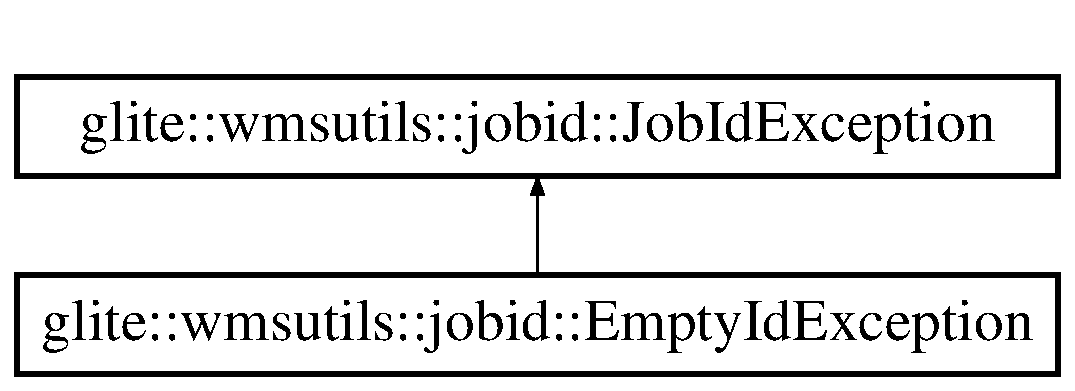
\includegraphics[height=2cm]{classglite_1_1wmsutils_1_1jobid_1_1EmptyIdException}
\end{center}
\end{figure}
\subsection*{Public Member Functions}
\begin{CompactItemize}
\item 
\hyperlink{classglite_1_1wmsutils_1_1jobid_1_1EmptyIdException_a0}{Empty\-Id\-Exception::Empty\-Id\-Exception} (const std::string \&file, int line, const std::string \&method, int code, const std::string \&field)
\end{CompactItemize}


\subsection{Detailed Description}
\hyperlink{classglite_1_1wmsutils_1_1jobid_1_1EmptyIdException}{Empty\-Id\-Exception} This Exception is thrown when the user tries to get information from a \hyperlink{classglite_1_1wmsutils_1_1jobid_1_1JobId}{Job\-Id} which has not been initialized yet, i.e tries to use the get$<$field name$>$ Methods 



\subsection{Member Function Documentation}
\hypertarget{classglite_1_1wmsutils_1_1jobid_1_1EmptyIdException_a0}{
\index{glite::wmsutils::jobid::EmptyIdException@{glite::wmsutils::jobid::Empty\-Id\-Exception}!EmptyIdException::EmptyIdException@{EmptyIdException::EmptyIdException}}
\index{EmptyIdException::EmptyIdException@{EmptyIdException::EmptyIdException}!glite::wmsutils::jobid::EmptyIdException@{glite::wmsutils::jobid::Empty\-Id\-Exception}}
\subsubsection[EmptyIdException::EmptyIdException]{\setlength{\rightskip}{0pt plus 5cm}glite::wmsutils::jobid::Empty\-Id\-Exception::Empty\-Id\-Exception::Empty\-Id\-Exception (const std::string \& {\em file}, int {\em line}, const std::string \& {\em method}, int {\em code}, const std::string \& {\em field})}}
\label{classglite_1_1wmsutils_1_1jobid_1_1EmptyIdException_a0}


Constructor \begin{Desc}
\item[Parameters:]
\begin{description}
\item[{\em file}]- The source file which has generated the Exception \item[{\em line}]- The line number in the source file where the Exception has been thrown \item[{\em method}]- The Name of the method which has thrown the Exception \item[{\em code}]- The Code of the Error raised \item[{\em field}]- The Empty filed requested for \end{description}
\end{Desc}


The documentation for this class was generated from the following file:\begin{CompactItemize}
\item 
\hyperlink{JobIdExceptions_8h}{Job\-Id\-Exceptions.h}\end{CompactItemize}

\hypertarget{classglite_1_1wmsutils_1_1jobid_1_1JobId}{
\section{glite::wmsutils::jobid::Job\-Id Class Reference}
\label{classglite_1_1wmsutils_1_1jobid_1_1JobId}\index{glite::wmsutils::jobid::JobId@{glite::wmsutils::jobid::JobId}}
}
{\tt \#include $<$Job\-Id.h$>$}

\subsection*{Public Member Functions}
\begin{CompactItemize}
\item 
void \hyperlink{classglite_1_1wmsutils_1_1jobid_1_1JobId_a0}{from\-String} (const std::string \&dg\_\-Job\-Id)
\item 
std::string \hyperlink{classglite_1_1wmsutils_1_1jobid_1_1JobId_a1}{to\-String} () const 
\item 
\hyperlink{classglite_1_1wmsutils_1_1jobid_1_1JobId_a2}{operator const edg\_\-wlc\_\-Job\-Id} () const 
\item 
\hyperlink{classglite_1_1wmsutils_1_1jobid_1_1JobId}{Job\-Id} \& \hyperlink{classglite_1_1wmsutils_1_1jobid_1_1JobId_a3}{operator=} (\hyperlink{classglite_1_1wmsutils_1_1jobid_1_1JobId}{Job\-Id} const \&)
\item 
\hyperlink{classglite_1_1wmsutils_1_1jobid_1_1JobId}{Job\-Id} \& \hyperlink{classglite_1_1wmsutils_1_1jobid_1_1JobId_a4}{operator=} (const \hyperlink{cjobid_8h_a2}{edg\_\-wlc\_\-Job\-Id} \&)
\item 
\hyperlink{cjobid_8h_a2}{edg\_\-wlc\_\-Job\-Id} \hyperlink{classglite_1_1wmsutils_1_1jobid_1_1JobId_a5}{get\-Id} () const 
\end{CompactItemize}
\begin{Indent}{\bf Constructors/Destructor}\par
\begin{CompactItemize}
\item 
\hyperlink{classglite_1_1wmsutils_1_1jobid_1_1JobId_z1_0}{Job\-Id} ()
\item 
\hyperlink{classglite_1_1wmsutils_1_1jobid_1_1JobId_z1_1}{Job\-Id} (const std::string \&\hyperlink{classjobid}{jobid})
\item 
\hyperlink{classglite_1_1wmsutils_1_1jobid_1_1JobId_z1_2}{Job\-Id} (const \hyperlink{classglite_1_1wmsutils_1_1jobid_1_1JobId}{Job\-Id} \&\hyperlink{classjobid}{jobid})
\item 
\hyperlink{classglite_1_1wmsutils_1_1jobid_1_1JobId_z1_3}{Job\-Id} (const \hyperlink{cjobid_8h_a2}{edg\_\-wlc\_\-Job\-Id} \&\hyperlink{classjobid}{jobid})
\item 
\hyperlink{classglite_1_1wmsutils_1_1jobid_1_1JobId_z1_4}{$\sim$Job\-Id} ()
\end{CompactItemize}
\end{Indent}
\begin{Indent}{\bf Miscellaneous}\par
\begin{CompactItemize}
\item 
void \hyperlink{classglite_1_1wmsutils_1_1jobid_1_1JobId_z3_0}{clear} ()
\item 
bool \hyperlink{classglite_1_1wmsutils_1_1jobid_1_1JobId_z3_1}{is\-Set} ()
\item 
void \hyperlink{classglite_1_1wmsutils_1_1jobid_1_1JobId_z3_2}{set\-Job\-Id} (const std::string \&lb\_\-server, int port=0, const std::string \&unique=\char`\"{}\char`\"{})
\end{CompactItemize}
\end{Indent}
\begin{Indent}{\bf Get Methods}\par
\begin{CompactItemize}
\item 
std::string \hyperlink{classglite_1_1wmsutils_1_1jobid_1_1JobId_z5_0}{get\-Server} () const 
\item 
std::string \hyperlink{classglite_1_1wmsutils_1_1jobid_1_1JobId_z5_1}{get\-Unique} () const 
\end{CompactItemize}
\end{Indent}
\subsection*{Friends}
\begin{CompactItemize}
\item 
bool \hyperlink{classglite_1_1wmsutils_1_1jobid_1_1JobId_n0}{operator$<$} (\hyperlink{classglite_1_1wmsutils_1_1jobid_1_1JobId}{Job\-Id} const \&lhs, \hyperlink{classglite_1_1wmsutils_1_1jobid_1_1JobId}{Job\-Id} const \&rhs)
\item 
bool \hyperlink{classglite_1_1wmsutils_1_1jobid_1_1JobId_n1}{operator==} (\hyperlink{classglite_1_1wmsutils_1_1jobid_1_1JobId}{Job\-Id} const \&lhs, \hyperlink{classglite_1_1wmsutils_1_1jobid_1_1JobId}{Job\-Id} const \&rhs)
\end{CompactItemize}


\subsection{Detailed Description}
Managing Identification, checking, retreiving info from a job File name: \hyperlink{JobId_8h}{Job\-Id.h} The \hyperlink{classglite_1_1wmsutils_1_1jobid_1_1JobId}{Job\-Id} class provides a representation of the Datagrid job identifier (dg\_\-job\-Id) and the methods for manipulating it. We remind that the format of the dg\_\-job\-Id is as follows: :/

\begin{Desc}
\item[Version:]0.1 \end{Desc}
\begin{Desc}
\item[Date:]15 April 2002 \end{Desc}
\begin{Desc}
\item[Author:]Alessandro Maraschini $<$\href{mailto:alessandro.maraschini@datamat.it}{\tt alessandro.maraschini@datamat.it}$>$ \end{Desc}




\subsection{Constructor \& Destructor Documentation}
\hypertarget{classglite_1_1wmsutils_1_1jobid_1_1JobId_z1_0}{
\index{glite::wmsutils::jobid::JobId@{glite::wmsutils::jobid::Job\-Id}!JobId@{JobId}}
\index{JobId@{JobId}!glite::wmsutils::jobid::JobId@{glite::wmsutils::jobid::Job\-Id}}
\subsubsection[JobId]{\setlength{\rightskip}{0pt plus 5cm}glite::wmsutils::jobid::Job\-Id::Job\-Id ()}}
\label{classglite_1_1wmsutils_1_1jobid_1_1JobId_z1_0}


Instantiates an empty \hyperlink{classglite_1_1wmsutils_1_1jobid_1_1JobId}{Job\-Id} object \hypertarget{classglite_1_1wmsutils_1_1jobid_1_1JobId_z1_1}{
\index{glite::wmsutils::jobid::JobId@{glite::wmsutils::jobid::Job\-Id}!JobId@{JobId}}
\index{JobId@{JobId}!glite::wmsutils::jobid::JobId@{glite::wmsutils::jobid::Job\-Id}}
\subsubsection[JobId]{\setlength{\rightskip}{0pt plus 5cm}glite::wmsutils::jobid::Job\-Id::Job\-Id (const std::string \& {\em jobid})}}
\label{classglite_1_1wmsutils_1_1jobid_1_1JobId_z1_1}


Instantiates a \hyperlink{classglite_1_1wmsutils_1_1jobid_1_1JobId}{Job\-Id} object from the passed dg\_\-job\-Id in string format. \begin{Desc}
\item[Parameters:]
\begin{description}
\item[{\em jobid}]a string representig a class\-Ad expression \end{description}
\end{Desc}
\begin{Desc}
\item[Exceptions:]
\begin{description}
\item[{\em Wrong\-Id\-Exception}]When a string is passed in a wrong format \end{description}
\end{Desc}
\hypertarget{classglite_1_1wmsutils_1_1jobid_1_1JobId_z1_2}{
\index{glite::wmsutils::jobid::JobId@{glite::wmsutils::jobid::Job\-Id}!JobId@{JobId}}
\index{JobId@{JobId}!glite::wmsutils::jobid::JobId@{glite::wmsutils::jobid::Job\-Id}}
\subsubsection[JobId]{\setlength{\rightskip}{0pt plus 5cm}glite::wmsutils::jobid::Job\-Id::Job\-Id (const \hyperlink{classglite_1_1wmsutils_1_1jobid_1_1JobId}{Job\-Id} \& {\em jobid})}}
\label{classglite_1_1wmsutils_1_1jobid_1_1JobId_z1_2}


Instantiates a \hyperlink{classglite_1_1wmsutils_1_1jobid_1_1JobId}{Job\-Id} object from the passed \hyperlink{classglite_1_1wmsutils_1_1jobid_1_1JobId}{Job\-Id} instance \begin{Desc}
\item[Parameters:]
\begin{description}
\item[{\em jobid}]a \hyperlink{classglite_1_1wmsutils_1_1jobid_1_1JobId}{Job\-Id} instance to copy from \end{description}
\end{Desc}
\begin{Desc}
\item[Exceptions:]
\begin{description}
\item[{\em Wrong\-Id\-Exception}]When a string is passed in a wrong format \end{description}
\end{Desc}
\hypertarget{classglite_1_1wmsutils_1_1jobid_1_1JobId_z1_3}{
\index{glite::wmsutils::jobid::JobId@{glite::wmsutils::jobid::Job\-Id}!JobId@{JobId}}
\index{JobId@{JobId}!glite::wmsutils::jobid::JobId@{glite::wmsutils::jobid::Job\-Id}}
\subsubsection[JobId]{\setlength{\rightskip}{0pt plus 5cm}glite::wmsutils::jobid::Job\-Id::Job\-Id (const \hyperlink{cjobid_8h_a2}{edg\_\-wlc\_\-Job\-Id} \& {\em jobid})}}
\label{classglite_1_1wmsutils_1_1jobid_1_1JobId_z1_3}


Instantiates a \hyperlink{classglite_1_1wmsutils_1_1jobid_1_1JobId}{Job\-Id} object from the passed \hyperlink{classglite_1_1wmsutils_1_1jobid_1_1JobId}{Job\-Id} internal reference \begin{Desc}
\item[Parameters:]
\begin{description}
\item[{\em jobid}]the \hyperlink{classglite_1_1wmsutils_1_1jobid_1_1JobId}{Job\-Id} internal reference \end{description}
\end{Desc}
\begin{Desc}
\item[Exceptions:]
\begin{description}
\item[{\em Wrong\-Id\-Exception}]When a string is passed in a wrong format \end{description}
\end{Desc}
\hypertarget{classglite_1_1wmsutils_1_1jobid_1_1JobId_z1_4}{
\index{glite::wmsutils::jobid::JobId@{glite::wmsutils::jobid::Job\-Id}!~JobId@{$\sim$JobId}}
\index{~JobId@{$\sim$JobId}!glite::wmsutils::jobid::JobId@{glite::wmsutils::jobid::Job\-Id}}
\subsubsection[$\sim$JobId]{\setlength{\rightskip}{0pt plus 5cm}glite::wmsutils::jobid::Job\-Id::$\sim$\hyperlink{classglite_1_1wmsutils_1_1jobid_1_1JobId}{Job\-Id} ()}}
\label{classglite_1_1wmsutils_1_1jobid_1_1JobId_z1_4}


Destructor Destroy the Job Id instance 

\subsection{Member Function Documentation}
\hypertarget{classglite_1_1wmsutils_1_1jobid_1_1JobId_z3_0}{
\index{glite::wmsutils::jobid::JobId@{glite::wmsutils::jobid::Job\-Id}!clear@{clear}}
\index{clear@{clear}!glite::wmsutils::jobid::JobId@{glite::wmsutils::jobid::Job\-Id}}
\subsubsection[clear]{\setlength{\rightskip}{0pt plus 5cm}void glite::wmsutils::jobid::Job\-Id::clear ()}}
\label{classglite_1_1wmsutils_1_1jobid_1_1JobId_z3_0}


Unsets the \hyperlink{classglite_1_1wmsutils_1_1jobid_1_1JobId}{Job\-Id} instance. Clear all it's memebers \hypertarget{classglite_1_1wmsutils_1_1jobid_1_1JobId_a0}{
\index{glite::wmsutils::jobid::JobId@{glite::wmsutils::jobid::Job\-Id}!fromString@{fromString}}
\index{fromString@{fromString}!glite::wmsutils::jobid::JobId@{glite::wmsutils::jobid::Job\-Id}}
\subsubsection[fromString]{\setlength{\rightskip}{0pt plus 5cm}void glite::wmsutils::jobid::Job\-Id::from\-String (const std::string \& {\em dg\_\-Job\-Id})}}
\label{classglite_1_1wmsutils_1_1jobid_1_1JobId_a0}


This method sets the \hyperlink{classglite_1_1wmsutils_1_1jobid_1_1JobId}{Job\-Id} instance from the \hyperlink{classglite_1_1wmsutils_1_1jobid_1_1JobId}{Job\-Id} in string format given as input. \begin{Desc}
\item[Parameters:]
\begin{description}
\item[{\em dg\_\-Job\-Id}]the string representing the job \end{description}
\end{Desc}
\begin{Desc}
\item[Exceptions:]
\begin{description}
\item[{\em Wrong\-Id\-Exception}]When a string is passed in a wrong format \end{description}
\end{Desc}
\hypertarget{classglite_1_1wmsutils_1_1jobid_1_1JobId_a5}{
\index{glite::wmsutils::jobid::JobId@{glite::wmsutils::jobid::Job\-Id}!getId@{getId}}
\index{getId@{getId}!glite::wmsutils::jobid::JobId@{glite::wmsutils::jobid::Job\-Id}}
\subsubsection[getId]{\setlength{\rightskip}{0pt plus 5cm}\hyperlink{cjobid_8h_a2}{edg\_\-wlc\_\-Job\-Id} glite::wmsutils::jobid::Job\-Id::get\-Id () const}}
\label{classglite_1_1wmsutils_1_1jobid_1_1JobId_a5}


Retrieve the internal id reference \begin{Desc}
\item[Returns:]the \hyperlink{classglite_1_1wmsutils_1_1jobid_1_1JobId}{Job\-Id} internal reference used by some LB methods \end{Desc}
\hypertarget{classglite_1_1wmsutils_1_1jobid_1_1JobId_z5_0}{
\index{glite::wmsutils::jobid::JobId@{glite::wmsutils::jobid::Job\-Id}!getServer@{getServer}}
\index{getServer@{getServer}!glite::wmsutils::jobid::JobId@{glite::wmsutils::jobid::Job\-Id}}
\subsubsection[getServer]{\setlength{\rightskip}{0pt plus 5cm}std::string glite::wmsutils::jobid::Job\-Id::get\-Server () const}}
\label{classglite_1_1wmsutils_1_1jobid_1_1JobId_z5_0}


\begin{Desc}
\item[Returns:]the LB address into its string format \end{Desc}
\begin{Desc}
\item[Exceptions:]
\begin{description}
\item[{\em Empty\-Id\-Exception}]If the job\-Id has not been initialised yet \end{description}
\end{Desc}
\hypertarget{classglite_1_1wmsutils_1_1jobid_1_1JobId_z5_1}{
\index{glite::wmsutils::jobid::JobId@{glite::wmsutils::jobid::Job\-Id}!getUnique@{getUnique}}
\index{getUnique@{getUnique}!glite::wmsutils::jobid::JobId@{glite::wmsutils::jobid::Job\-Id}}
\subsubsection[getUnique]{\setlength{\rightskip}{0pt plus 5cm}std::string glite::wmsutils::jobid::Job\-Id::get\-Unique () const}}
\label{classglite_1_1wmsutils_1_1jobid_1_1JobId_z5_1}


\begin{Desc}
\item[Returns:]the Unique string into its string format \end{Desc}
\begin{Desc}
\item[Exceptions:]
\begin{description}
\item[{\em Empty\-Id\-Exception}]If the job\-Id has not been initialised yet \end{description}
\end{Desc}
\hypertarget{classglite_1_1wmsutils_1_1jobid_1_1JobId_z3_1}{
\index{glite::wmsutils::jobid::JobId@{glite::wmsutils::jobid::Job\-Id}!isSet@{isSet}}
\index{isSet@{isSet}!glite::wmsutils::jobid::JobId@{glite::wmsutils::jobid::Job\-Id}}
\subsubsection[isSet]{\setlength{\rightskip}{0pt plus 5cm}bool glite::wmsutils::jobid::Job\-Id::is\-Set ()\hspace{0.3cm}{\tt  \mbox{[}inline\mbox{]}}}}
\label{classglite_1_1wmsutils_1_1jobid_1_1JobId_z3_1}


Check wheater the job\-Id has been already created (true) or not (false) \begin{Desc}
\item[Returns:]true (job\-Id created) or false (job\-Id not yet created) \end{Desc}
\hypertarget{classglite_1_1wmsutils_1_1jobid_1_1JobId_a2}{
\index{glite::wmsutils::jobid::JobId@{glite::wmsutils::jobid::Job\-Id}!operator const edg_wlc_JobId@{operator const edg\_\-wlc\_\-JobId}}
\index{operator const edg_wlc_JobId@{operator const edg\_\-wlc\_\-JobId}!glite::wmsutils::jobid::JobId@{glite::wmsutils::jobid::Job\-Id}}
\subsubsection[operator const edg\_\-wlc\_\-JobId]{\setlength{\rightskip}{0pt plus 5cm}glite::wmsutils::jobid::Job\-Id::operator const \hyperlink{cjobid_8h_a2}{edg\_\-wlc\_\-Job\-Id} () const\hspace{0.3cm}{\tt  \mbox{[}inline\mbox{]}}}}
\label{classglite_1_1wmsutils_1_1jobid_1_1JobId_a2}


casting operator \hypertarget{classglite_1_1wmsutils_1_1jobid_1_1JobId_a4}{
\index{glite::wmsutils::jobid::JobId@{glite::wmsutils::jobid::Job\-Id}!operator=@{operator=}}
\index{operator=@{operator=}!glite::wmsutils::jobid::JobId@{glite::wmsutils::jobid::Job\-Id}}
\subsubsection[operator=]{\setlength{\rightskip}{0pt plus 5cm}\hyperlink{classglite_1_1wmsutils_1_1jobid_1_1JobId}{Job\-Id}\& glite::wmsutils::jobid::Job\-Id::operator= (const \hyperlink{cjobid_8h_a2}{edg\_\-wlc\_\-Job\-Id} \&)}}
\label{classglite_1_1wmsutils_1_1jobid_1_1JobId_a4}


Operator \char`\"{}=\char`\"{} create a deep copy of the \hyperlink{classglite_1_1wmsutils_1_1jobid_1_1JobId}{Job\-Id} instance \hypertarget{classglite_1_1wmsutils_1_1jobid_1_1JobId_a3}{
\index{glite::wmsutils::jobid::JobId@{glite::wmsutils::jobid::Job\-Id}!operator=@{operator=}}
\index{operator=@{operator=}!glite::wmsutils::jobid::JobId@{glite::wmsutils::jobid::Job\-Id}}
\subsubsection[operator=]{\setlength{\rightskip}{0pt plus 5cm}\hyperlink{classglite_1_1wmsutils_1_1jobid_1_1JobId}{Job\-Id}\& glite::wmsutils::jobid::Job\-Id::operator= (\hyperlink{classglite_1_1wmsutils_1_1jobid_1_1JobId}{Job\-Id} const \&)}}
\label{classglite_1_1wmsutils_1_1jobid_1_1JobId_a3}


Operator \char`\"{}=\char`\"{} create a deep copy of the \hyperlink{classglite_1_1wmsutils_1_1jobid_1_1JobId}{Job\-Id} instance \hypertarget{classglite_1_1wmsutils_1_1jobid_1_1JobId_z3_2}{
\index{glite::wmsutils::jobid::JobId@{glite::wmsutils::jobid::Job\-Id}!setJobId@{setJobId}}
\index{setJobId@{setJobId}!glite::wmsutils::jobid::JobId@{glite::wmsutils::jobid::Job\-Id}}
\subsubsection[setJobId]{\setlength{\rightskip}{0pt plus 5cm}void glite::wmsutils::jobid::Job\-Id::set\-Job\-Id (const std::string \& {\em lb\_\-server}, int {\em port} = 0, const std::string \& {\em unique} = \char`\"{}\char`\"{})}}
\label{classglite_1_1wmsutils_1_1jobid_1_1JobId_z3_2}


Set the \hyperlink{classglite_1_1wmsutils_1_1jobid_1_1JobId}{Job\-Id} instance according to the LB and RB server addresses and the unique string passed as input parameters. \begin{Desc}
\item[Parameters:]
\begin{description}
\item[{\em lb\_\-server}]Loggin and Bookkeeping server address \item[{\em port}]Loggin and Bookkeeping port ( dafault value is 9000 ) \item[{\em unique}]A Unique identification ( automatically generatad by md5 protocol ) \end{description}
\end{Desc}
\begin{Desc}
\item[Exceptions:]
\begin{description}
\item[{\em Wrong\-Id\-Exception}]When one parameter has been passed in a wrong format \end{description}
\end{Desc}
\hypertarget{classglite_1_1wmsutils_1_1jobid_1_1JobId_a1}{
\index{glite::wmsutils::jobid::JobId@{glite::wmsutils::jobid::Job\-Id}!toString@{toString}}
\index{toString@{toString}!glite::wmsutils::jobid::JobId@{glite::wmsutils::jobid::Job\-Id}}
\subsubsection[toString]{\setlength{\rightskip}{0pt plus 5cm}std::string glite::wmsutils::jobid::Job\-Id::to\-String () const}}
\label{classglite_1_1wmsutils_1_1jobid_1_1JobId_a1}


Converts the job\-Id into a string \begin{Desc}
\item[Returns:]the string representation of a \hyperlink{classglite_1_1wmsutils_1_1jobid_1_1JobId}{Job\-Id} \end{Desc}


\subsection{Friends And Related Function Documentation}
\hypertarget{classglite_1_1wmsutils_1_1jobid_1_1JobId_n0}{
\index{glite::wmsutils::jobid::JobId@{glite::wmsutils::jobid::Job\-Id}!operator<@{operator$<$}}
\index{operator<@{operator$<$}!glite::wmsutils::jobid::JobId@{glite::wmsutils::jobid::Job\-Id}}
\subsubsection[operator$<$]{\setlength{\rightskip}{0pt plus 5cm}bool operator$<$ (\hyperlink{classglite_1_1wmsutils_1_1jobid_1_1JobId}{Job\-Id} const \& {\em lhs}, \hyperlink{classglite_1_1wmsutils_1_1jobid_1_1JobId}{Job\-Id} const \& {\em rhs})\hspace{0.3cm}{\tt  \mbox{[}friend\mbox{]}}}}
\label{classglite_1_1wmsutils_1_1jobid_1_1JobId_n0}


Operator \char`\"{}$<$\char`\"{} \hypertarget{classglite_1_1wmsutils_1_1jobid_1_1JobId_n1}{
\index{glite::wmsutils::jobid::JobId@{glite::wmsutils::jobid::Job\-Id}!operator==@{operator==}}
\index{operator==@{operator==}!glite::wmsutils::jobid::JobId@{glite::wmsutils::jobid::Job\-Id}}
\subsubsection[operator==]{\setlength{\rightskip}{0pt plus 5cm}bool operator== (\hyperlink{classglite_1_1wmsutils_1_1jobid_1_1JobId}{Job\-Id} const \& {\em lhs}, \hyperlink{classglite_1_1wmsutils_1_1jobid_1_1JobId}{Job\-Id} const \& {\em rhs})\hspace{0.3cm}{\tt  \mbox{[}friend\mbox{]}}}}
\label{classglite_1_1wmsutils_1_1jobid_1_1JobId_n1}


Operator \char`\"{}==\char`\"{} 

The documentation for this class was generated from the following file:\begin{CompactItemize}
\item 
\hyperlink{JobId_8h}{Job\-Id.h}\end{CompactItemize}

\hypertarget{classglite_1_1wmsutils_1_1jobid_1_1JobIdException}{
\section{glite::wmsutils::jobid::Job\-Id\-Exception Class Reference}
\label{classglite_1_1wmsutils_1_1jobid_1_1JobIdException}\index{glite::wmsutils::jobid::JobIdException@{glite::wmsutils::jobid::JobIdException}}
}
{\tt \#include $<$Job\-Id\-Exceptions.h$>$}

Inheritance diagram for glite::wmsutils::jobid::Job\-Id\-Exception::\begin{figure}[H]
\begin{center}
\leavevmode
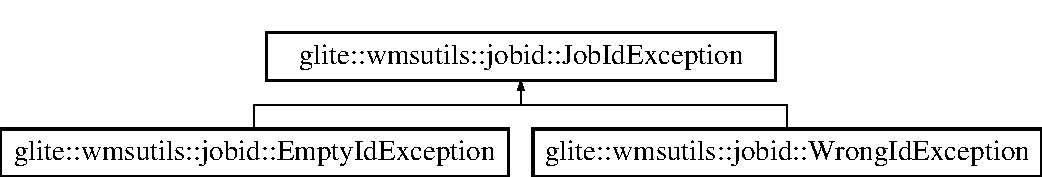
\includegraphics[height=2cm]{classglite_1_1wmsutils_1_1jobid_1_1JobIdException}
\end{center}
\end{figure}
\subsection*{Public Member Functions}
\begin{CompactItemize}
\item 
\hyperlink{classglite_1_1wmsutils_1_1jobid_1_1JobIdException_a0}{Job\-Id\-Exception} (const std::string \&file, int line, const std::string \&method, int code, const std::string \&exception\_\-name)
\end{CompactItemize}


\subsection{Detailed Description}
\hyperlink{classglite_1_1wmsutils_1_1jobid_1_1JobIdException}{Job\-Id\-Exception} - Exception thrown by \hyperlink{classglite_1_1wmsutils_1_1jobid_1_1JobId}{Job\-Id} Class \begin{Desc}
\item[Version:]0.1 \end{Desc}
\begin{Desc}
\item[Date:]15 April 2002 \end{Desc}
\begin{Desc}
\item[Author:]Alessandro Maraschini $<$\href{mailto:alessandro.maraschini@datamat.it}{\tt alessandro.maraschini@datamat.it}$>$ \end{Desc}




\subsection{Constructor \& Destructor Documentation}
\hypertarget{classglite_1_1wmsutils_1_1jobid_1_1JobIdException_a0}{
\index{glite::wmsutils::jobid::JobIdException@{glite::wmsutils::jobid::Job\-Id\-Exception}!JobIdException@{JobIdException}}
\index{JobIdException@{JobIdException}!glite::wmsutils::jobid::JobIdException@{glite::wmsutils::jobid::Job\-Id\-Exception}}
\subsubsection[JobIdException]{\setlength{\rightskip}{0pt plus 5cm}glite::wmsutils::jobid::Job\-Id\-Exception::Job\-Id\-Exception (const std::string \& {\em file}, int {\em line}, const std::string \& {\em method}, int {\em code}, const std::string \& {\em exception\_\-name})}}
\label{classglite_1_1wmsutils_1_1jobid_1_1JobIdException_a0}


Update all mandatory Exception Information 

The documentation for this class was generated from the following file:\begin{CompactItemize}
\item 
\hyperlink{JobIdExceptions_8h}{Job\-Id\-Exceptions.h}\end{CompactItemize}

\hypertarget{classglite_1_1wmsutils_1_1jobid_1_1WrongIdException}{
\section{glite::wmsutils::jobid::Wrong\-Id\-Exception Class Reference}
\label{classglite_1_1wmsutils_1_1jobid_1_1WrongIdException}\index{glite::wmsutils::jobid::WrongIdException@{glite::wmsutils::jobid::WrongIdException}}
}
{\tt \#include $<$Job\-Id\-Exceptions.h$>$}

Inheritance diagram for glite::wmsutils::jobid::Wrong\-Id\-Exception::\begin{figure}[H]
\begin{center}
\leavevmode
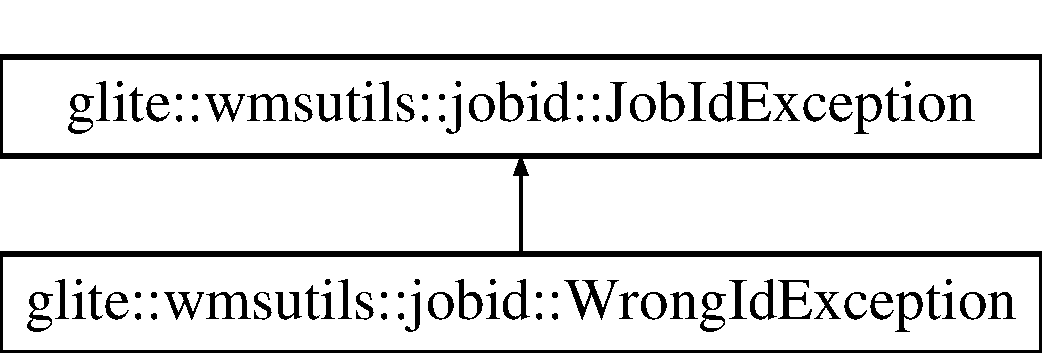
\includegraphics[height=2cm]{classglite_1_1wmsutils_1_1jobid_1_1WrongIdException}
\end{center}
\end{figure}
\subsection*{Public Member Functions}
\begin{CompactItemize}
\item 
\hyperlink{classglite_1_1wmsutils_1_1jobid_1_1WrongIdException_a0}{Wrong\-Id\-Exception} (const std::string \&file, int line, const std::string \&method, int code)
\end{CompactItemize}


\subsection{Detailed Description}
Wrong\-Id\-Field\-Exception This Exception is thrown when a Job Id syntax error is found A valid Job Identification string should be made as follows: :/  



\subsection{Constructor \& Destructor Documentation}
\hypertarget{classglite_1_1wmsutils_1_1jobid_1_1WrongIdException_a0}{
\index{glite::wmsutils::jobid::WrongIdException@{glite::wmsutils::jobid::Wrong\-Id\-Exception}!WrongIdException@{WrongIdException}}
\index{WrongIdException@{WrongIdException}!glite::wmsutils::jobid::WrongIdException@{glite::wmsutils::jobid::Wrong\-Id\-Exception}}
\subsubsection[WrongIdException]{\setlength{\rightskip}{0pt plus 5cm}glite::wmsutils::jobid::Wrong\-Id\-Exception::Wrong\-Id\-Exception (const std::string \& {\em file}, int {\em line}, const std::string \& {\em method}, int {\em code})}}
\label{classglite_1_1wmsutils_1_1jobid_1_1WrongIdException_a0}


Constructor \begin{Desc}
\item[Parameters:]
\begin{description}
\item[{\em file}]- The source file which has generated the Exception \item[{\em line}]- The line number in the source file where the Exception has been thrown \item[{\em method}]- The Name of the method which has thrown the Exception \item[{\em code}]- The Code of the Error raised \item[{\em field}]- The wrong expression catched \end{description}
\end{Desc}


The documentation for this class was generated from the following file:\begin{CompactItemize}
\item 
\hyperlink{JobIdExceptions_8h}{Job\-Id\-Exceptions.h}\end{CompactItemize}


}


\subsection{BrokerInfo Access API---C++ binding}
\label{brki}
{
\renewenvironment{CompactList}{\itemize\itemsep -2pt}{\enditemize}
\def\section#1{}
\renewcommand{\contentsline}[4]{{\bf #2}\leaders\hbox{.}\hfill #3}
The documentation of C$++$ BrokerInfo Access API presented in this section was generated automatically from the
comments in the API header files by Doxygen. The package providing the BrokerInfo Access API is 
{\verb!org.glite.wms.brokerinfo-access!}.

The class hierarchy is depicted in the following list.
\section{Brokerinfo access Class List}
Here are the classes, structs, unions and interfaces with brief descriptions:\begin{CompactList}
\item\contentsline{section}{\hyperlink{classBrokerInfo}{Broker\-Info} (Parses .Broker\-Info file containing job submission parameters )}{\pageref{classBrokerInfo}}{}
\item\contentsline{section}{\hyperlink{classBrokerInfoEx}{Broker\-Info\-Ex} }{\pageref{classBrokerInfoEx}}{}
\end{CompactList}

}

\noindent The BrokerInfo Access API classes are described in the
following sections.
{
% save previous definitions for use in new macros
\let\dsection=\section
\let\dsubsection=\subsection
\let\dsubsubsection=\subsubsection

% change the sections definition to reflect the actual hierarchy
%  - section is just one in each included file
\renewcommand{\section}[1]{\dsubsubsection{#1}}
%  - subsections are for member section headings (constructors, data, ...)
\renewcommand{\subsection}[2]{\ifx*#1
\dsubsubsection*{#2}\def\zbytek{}
\else
\dsubsubsection*{#1}\def\zbytek{#2}\fi
\zbytek}
%  - subsubsections are for particular class members
\def\eatbraces#1]{}
\def\dosubsubsection#1{\par
  \vskip 10pt\framebox{\begin{minipage}{\linewidth}{\hangindent=20pt\noindent\bf #1\par}\end{minipage}}\vskip-2pt}
\renewcommand{\subsubsection}[2]{\ifx*#1
  \dosubsubsection{#2}\def\zbytek{}
\else\ifx[#1
  \def\zbytek{\expandafter\dosubsubsection\eatbraces}
\else
  \dosubsubsection{#1}\def\zbytek{#2}
\fi\fi
\zbytek}

%\let\ddescription=\description
%\let\denddescription=\enddescription
%\renewenvironment{description}{\list{}{\labelwidth 5cm\leftmargin 3cm}}{\endlist}


\let\ddescription=\description
\let\denddescription=\enddescription
\renewenvironment{description}{\list{}{\labelwidth 4cm\leftmargin 4cm}}{\endlist}
% documentation for particular classes

\hypertarget{classBrokerInfo}{
\section{Broker\-Info Class Reference}
\label{classBrokerInfo}\index{BrokerInfo@{BrokerInfo}}
}
parses .Broker\-Info file containing job submission parameters  


{\tt \#include $<$Broker\-Info.h$>$}

\subsection*{Public Member Functions}
\begin{CompactItemize}
\item 
\hyperlink{classBrokerInfo_a0}{$\sim$Broker\-Info} (void)
\item 
std::string \hyperlink{classBrokerInfo_a1}{get\-BIFile\-Name} (void)
\item 
\hyperlink{bi__result_8h_a2}{BI\_\-Result} \hyperlink{classBrokerInfo_a2}{get\-CE} (std::string \&CE)
\item 
\hyperlink{bi__result_8h_a2}{BI\_\-Result} \hyperlink{classBrokerInfo_a3}{get\-Data\-Access\-Protocol} (std::vector$<$ std::string $>$ \&DAPs)
\item 
\hyperlink{bi__result_8h_a2}{BI\_\-Result} \hyperlink{classBrokerInfo_a4}{get\-LFN2SFN} (std::string LFN, std::vector$<$ std::string $>$ \&SFNs)
\item 
\hyperlink{bi__result_8h_a2}{BI\_\-Result} \hyperlink{classBrokerInfo_a5}{get\-SEs} (std::vector$<$ std::string $>$ \&SEs)
\item 
\hyperlink{bi__result_8h_a2}{BI\_\-Result} \hyperlink{classBrokerInfo_a6}{get\-SEProtocols} (std::string SE, std::vector$<$ std::string $>$ \&SEProtos)
\item 
\hyperlink{bi__result_8h_a2}{BI\_\-Result} \hyperlink{classBrokerInfo_a7}{get\-SEPort} (std::string SE, std::string SEProtocol, std::string \&SEPort)
\item 
\hyperlink{bi__result_8h_a2}{BI\_\-Result} \hyperlink{classBrokerInfo_a8}{get\-Close\-SEs} (std::vector$<$ std::string $>$ \&SEs)
\item 
\hyperlink{bi__result_8h_a2}{BI\_\-Result} \hyperlink{classBrokerInfo_a9}{get\-SEMount\-Point} (std::string Close\-SE, std::string \&SEMount)
\item 
\hyperlink{bi__result_8h_a2}{BI\_\-Result} \hyperlink{classBrokerInfo_a10}{get\-SEFree\-Space} (std::string Close\-SE, std::string \&SEFree\-Space)
\item 
\hyperlink{bi__result_8h_a2}{BI\_\-Result} \hyperlink{classBrokerInfo_a11}{get\-Input\-Data} (std::vector$<$ std::string $>$ \&LFNs)
\item 
\hyperlink{bi__result_8h_a2}{BI\_\-Result} \hyperlink{classBrokerInfo_a12}{get\-Virtual\-Organization} (std::string \&VO)
\item 
int \hyperlink{classBrokerInfo_a13}{parser} (std::string \&outbuffer)
\end{CompactItemize}
\subsection*{Static Public Member Functions}
\begin{CompactItemize}
\item 
\hyperlink{classBrokerInfo}{Broker\-Info} $\ast$ \hyperlink{classBrokerInfo_e0}{instance} (void)
\end{CompactItemize}


\subsection{Detailed Description}
parses .Broker\-Info file containing job submission parameters 

\begin{Desc}
\item[Parameters:]
\begin{description}
\item[{\em Broker\-Info\-File\_\-}]holds the fullpath of the brokerinfo file \item[{\em fbrokerinfo\_\-}]handler to the brokerinfo file \item[{\em mbrokerinfo\_\-}]handler to the brokerinfo memory info \item[{\em instance\_\-}]it points to the current instance. this class is intended so to be instantiated only once (singleton). \end{description}
\end{Desc}




\subsection{Constructor \& Destructor Documentation}
\hypertarget{classBrokerInfo_a0}{
\index{BrokerInfo@{Broker\-Info}!~BrokerInfo@{$\sim$BrokerInfo}}
\index{~BrokerInfo@{$\sim$BrokerInfo}!BrokerInfo@{Broker\-Info}}
\subsubsection[$\sim$BrokerInfo]{\setlength{\rightskip}{0pt plus 5cm}Broker\-Info::$\sim$\hyperlink{classBrokerInfo}{Broker\-Info} (void)}}
\label{classBrokerInfo_a0}


Destructor. 

\subsection{Member Function Documentation}
\hypertarget{classBrokerInfo_a1}{
\index{BrokerInfo@{Broker\-Info}!getBIFileName@{getBIFileName}}
\index{getBIFileName@{getBIFileName}!BrokerInfo@{Broker\-Info}}
\subsubsection[getBIFileName]{\setlength{\rightskip}{0pt plus 5cm}std::string Broker\-Info::get\-BIFile\-Name (void)}}
\label{classBrokerInfo_a1}


the Broker\-Info file to parse. \hypertarget{classBrokerInfo_a2}{
\index{BrokerInfo@{Broker\-Info}!getCE@{getCE}}
\index{getCE@{getCE}!BrokerInfo@{Broker\-Info}}
\subsubsection[getCE]{\setlength{\rightskip}{0pt plus 5cm}\hyperlink{bi__result_8h_a2}{BI\_\-Result} Broker\-Info::get\-CE (std::string \& {\em CE})}}
\label{classBrokerInfo_a2}


\begin{Desc}
\item[Returns:]CE (Computing Element) Info. @param CE The Resource\-ID of the Computing Element to be returned. @return BI\_\-SUCCESS, or BI\_\-ERROR if the operation failed \end{Desc}
\hypertarget{classBrokerInfo_a8}{
\index{BrokerInfo@{Broker\-Info}!getCloseSEs@{getCloseSEs}}
\index{getCloseSEs@{getCloseSEs}!BrokerInfo@{Broker\-Info}}
\subsubsection[getCloseSEs]{\setlength{\rightskip}{0pt plus 5cm}\hyperlink{bi__result_8h_a2}{BI\_\-Result} Broker\-Info::get\-Close\-SEs (std::vector$<$ std::string $>$ \& {\em SEs})}}
\label{classBrokerInfo_a8}


\begin{Desc}
\item[Returns:]SE's protocol port number @param SE Vector of SEs close to the given CE. @return BI\_\-SUCCESS, or BI\_\-ERROR if the operation failed \end{Desc}
\hypertarget{classBrokerInfo_a3}{
\index{BrokerInfo@{Broker\-Info}!getDataAccessProtocol@{getDataAccessProtocol}}
\index{getDataAccessProtocol@{getDataAccessProtocol}!BrokerInfo@{Broker\-Info}}
\subsubsection[getDataAccessProtocol]{\setlength{\rightskip}{0pt plus 5cm}\hyperlink{bi__result_8h_a2}{BI\_\-Result} Broker\-Info::get\-Data\-Access\-Protocol (std::vector$<$ std::string $>$ \& {\em DAPs})}}
\label{classBrokerInfo_a3}


\begin{Desc}
\item[Returns:]Data Access Protocol list @param DAPs Vector of Data Access Protocols specified by the user. @return BI\_\-SUCCESS, or BI\_\-ERROR if the operation failed \end{Desc}
\hypertarget{classBrokerInfo_a11}{
\index{BrokerInfo@{Broker\-Info}!getInputData@{getInputData}}
\index{getInputData@{getInputData}!BrokerInfo@{Broker\-Info}}
\subsubsection[getInputData]{\setlength{\rightskip}{0pt plus 5cm}\hyperlink{bi__result_8h_a2}{BI\_\-Result} Broker\-Info::get\-Input\-Data (std::vector$<$ std::string $>$ \& {\em LFNs})}}
\label{classBrokerInfo_a11}


\begin{Desc}
\item[Returns:]Input\-Data list @param LFN/GUID/LFC vector. @return BI\_\-SUCCESS, or BI\_\-ERROR if the operation failed \end{Desc}
\hypertarget{classBrokerInfo_a4}{
\index{BrokerInfo@{Broker\-Info}!getLFN2SFN@{getLFN2SFN}}
\index{getLFN2SFN@{getLFN2SFN}!BrokerInfo@{Broker\-Info}}
\subsubsection[getLFN2SFN]{\setlength{\rightskip}{0pt plus 5cm}\hyperlink{bi__result_8h_a2}{BI\_\-Result} Broker\-Info::get\-LFN2SFN (std::string {\em LFN}, std::vector$<$ std::string $>$ \& {\em SFNs})}}
\label{classBrokerInfo_a4}


\begin{Desc}
\item[Returns:]LFN to SFN mapping @param LFN String of LFN specified. @param SFNs Vector of corresponding SFNs. @return BI\_\-SUCCESS, or BI\_\-ERROR if the operation failed \end{Desc}
\hypertarget{classBrokerInfo_a10}{
\index{BrokerInfo@{Broker\-Info}!getSEFreeSpace@{getSEFreeSpace}}
\index{getSEFreeSpace@{getSEFreeSpace}!BrokerInfo@{Broker\-Info}}
\subsubsection[getSEFreeSpace]{\setlength{\rightskip}{0pt plus 5cm}\hyperlink{bi__result_8h_a2}{BI\_\-Result} Broker\-Info::get\-SEFree\-Space (std::string {\em Close\-SE}, std::string \& {\em SEFree\-Space})}}
\label{classBrokerInfo_a10}


\begin{Desc}
\item[Returns:]SE Free\-Space for the specific Close\-SE returned by $\ast$  get\-Close\-SEs method. $\ast$ @param SEFree\-Space string of SE free space. $\ast$ @return BI\_\-SUCCESS, or BI\_\-ERROR if the operation failed \end{Desc}
\hypertarget{classBrokerInfo_a9}{
\index{BrokerInfo@{Broker\-Info}!getSEMountPoint@{getSEMountPoint}}
\index{getSEMountPoint@{getSEMountPoint}!BrokerInfo@{Broker\-Info}}
\subsubsection[getSEMountPoint]{\setlength{\rightskip}{0pt plus 5cm}\hyperlink{bi__result_8h_a2}{BI\_\-Result} Broker\-Info::get\-SEMount\-Point (std::string {\em Close\-SE}, std::string \& {\em SEMount})}}
\label{classBrokerInfo_a9}


\begin{Desc}
\item[Returns:]SE Mount\-Point for the specific Close\-SE returned by  get\-Close\-SEs method. @param SEMount string of SE mount point. @return BI\_\-SUCCESS, or BI\_\-ERROR if the operation failed \end{Desc}
\hypertarget{classBrokerInfo_a7}{
\index{BrokerInfo@{Broker\-Info}!getSEPort@{getSEPort}}
\index{getSEPort@{getSEPort}!BrokerInfo@{Broker\-Info}}
\subsubsection[getSEPort]{\setlength{\rightskip}{0pt plus 5cm}\hyperlink{bi__result_8h_a2}{BI\_\-Result} Broker\-Info::get\-SEPort (std::string {\em SE}, std::string {\em SEProtocol}, std::string \& {\em SEPort})}}
\label{classBrokerInfo_a7}


\begin{Desc}
\item[Returns:]SE Ports list ordered following the order of SEs  by get\-SEs @param SEPorts Vector of ports used by SEs. @return BI\_\-SUCCESS, or BI\_\-ERROR if the operation failed \end{Desc}
\hypertarget{classBrokerInfo_a6}{
\index{BrokerInfo@{Broker\-Info}!getSEProtocols@{getSEProtocols}}
\index{getSEProtocols@{getSEProtocols}!BrokerInfo@{Broker\-Info}}
\subsubsection[getSEProtocols]{\setlength{\rightskip}{0pt plus 5cm}\hyperlink{bi__result_8h_a2}{BI\_\-Result} Broker\-Info::get\-SEProtocols (std::string {\em SE}, std::vector$<$ std::string $>$ \& {\em SEProtos})}}
\label{classBrokerInfo_a6}


\begin{Desc}
\item[Returns:]SE Protocols list ordered following the order of SEs  by get\-SEs @param SEProtcs Vector of protocols supported by SEs. @return BI\_\-SUCCESS, or BI\_\-ERROR if the operation failed \end{Desc}
\hypertarget{classBrokerInfo_a5}{
\index{BrokerInfo@{Broker\-Info}!getSEs@{getSEs}}
\index{getSEs@{getSEs}!BrokerInfo@{Broker\-Info}}
\subsubsection[getSEs]{\setlength{\rightskip}{0pt plus 5cm}\hyperlink{bi__result_8h_a2}{BI\_\-Result} Broker\-Info::get\-SEs (std::vector$<$ std::string $>$ \& {\em SEs})}}
\label{classBrokerInfo_a5}


\begin{Desc}
\item[Returns:]SE (Storage Element) list @param SEs Vector of SEs serving PFNs. @return BI\_\-SUCCESS, or BI\_\-ERROR if the operation failed \end{Desc}
\hypertarget{classBrokerInfo_a12}{
\index{BrokerInfo@{Broker\-Info}!getVirtualOrganization@{getVirtualOrganization}}
\index{getVirtualOrganization@{getVirtualOrganization}!BrokerInfo@{Broker\-Info}}
\subsubsection[getVirtualOrganization]{\setlength{\rightskip}{0pt plus 5cm}\hyperlink{bi__result_8h_a2}{BI\_\-Result} Broker\-Info::get\-Virtual\-Organization (std::string \& {\em VO})}}
\label{classBrokerInfo_a12}


\begin{Desc}
\item[Returns:]Virtual Organization string @param VO string. @return BI\_\-SUCCESS, or BI\_\-ERROR if the operation failed \end{Desc}
\hypertarget{classBrokerInfo_e0}{
\index{BrokerInfo@{Broker\-Info}!instance@{instance}}
\index{instance@{instance}!BrokerInfo@{Broker\-Info}}
\subsubsection[instance]{\setlength{\rightskip}{0pt plus 5cm}\hyperlink{classBrokerInfo}{Broker\-Info}$\ast$ Broker\-Info::instance (void)\hspace{0.3cm}{\tt  \mbox{[}static\mbox{]}}}}
\label{classBrokerInfo_e0}


the handle to the instantiated object. \hypertarget{classBrokerInfo_a13}{
\index{BrokerInfo@{Broker\-Info}!parser@{parser}}
\index{parser@{parser}!BrokerInfo@{Broker\-Info}}
\subsubsection[parser]{\setlength{\rightskip}{0pt plus 5cm}int Broker\-Info::parser (std::string \& {\em outbuffer})}}
\label{classBrokerInfo_a13}


utilities 

The documentation for this class was generated from the following file:\begin{CompactItemize}
\item 
\hyperlink{BrokerInfo_8h}{Broker\-Info.h}\end{CompactItemize}

\hypertarget{classBrokerInfoEx}{
\section{Broker\-Info\-Ex Class Reference}
\label{classBrokerInfoEx}\index{BrokerInfoEx@{BrokerInfoEx}}
}
{\tt \#include $<$Broker\-Info.h$>$}



The documentation for this class was generated from the following file:\begin{CompactItemize}
\item 
\hyperlink{BrokerInfo_8h}{Broker\-Info.h}\end{CompactItemize}


}




\newpage
\section{Known Problems and Caveats}
\label{caveats}
%\section{Known Problems and Caveats}

\subsection{Submission Failures Analysis}

Analysis of failed job's state can be carried out through the check of the consistency and completeness of the 
job related events returned by the \textit{glite-job-logging-info} command. A further verification if needed, should be 
then performed on the retrieved output files produced by the jobs (if any) and through the inspection of the log 
files ad debugging information traced by the various system components.
As explained in section~\ref{cli} to get the logging information about a job you need to issue the following command:

\smallskip
{\scriptsize{\verb!glite-job-logging-info <job Identifier>!}}
\smallskip


Since the output of the command could be copious we advice usage of the -output option too to redirect it 
to a given file:

\smallskip
{\scriptsize{\verb!glite-job-logging-info --output <my_file> <job Identifier>!}}
\smallskip

Augmenting the verbosity allows then to get more detailed information (the job descriptions at the various stages are 
also included):

\smallskip
{\scriptsize{\verb!glite-job-logging-info -v 3 --output <my_file> <job Identifier>!}}
\smallskip

Before using the \textit{glite-job-logging-info} command, it is in some cases useful a check to the \textit{glite-job-status} 
output that can contain information about the cause of a job failure (e.g. in the "Status Reason" field). 
As explained in section~\ref{cli} to get the status information about a job you need to issue the following command:

\smallskip
{\scriptsize{\verb!glite-job-status -v 2 <job Identifier>!}}
\smallskip

As said at the beginning of this section another way for analysing submission failures is to inspect the standard output 
and error of the job generated on the Worker Node and retrieved on the WMS-UI machine through the \textit{glite-job-output} 
command.  A typical example of errors that can be detected in this way is when the users submits a script that in turn 
tries to start another script or an executable. If e.g. the submitted scripts is like:


\smallskip
\begin{verbatim}

#!/bin/sh
# Use the coincidence file to compare the measurements
curdir=`pwd`
${curdir}/lecture_new_gome_V2_sel1_PT_10
idl appli.pro

\end{verbatim}
\smallskip


Upon job abortion, the error message received through the OutputSandbox retrieval is:

\smallskip
{\scriptsize{\verb!./demo_june: /home/eo004/3042/lecture_new_gome_V2_sel1_PT_10: Permission denied!}}
\smallskip

The reason for this error is that globus-url-copy (used for the InputSanbox files staging) in general doesn't preserve 
the \emph{x} flag so the script specified as Executable in the JDL (on which chmod +x is done automatically by the 
JobWrapper), should perform a chmod +x for all the executable files (\textit{lecture\_new\_gome\_V2\_sel1\_PT\_10} in 
this example) transferred within the InputSandbox of the job.


Hereafter is reported a brief description of the job events that can help when investigating a failure as suggested above.


\subsubsection{Job Event Types}

Hereafter is reported the list of job event types that could be returned to the user by the 
\textit{glite-job-logging-info} command. They are organized in several categories:

\smallskip

Events concerning a job transfer between components:
\begin{itemize}
 	\item \textbf{JobTransfer}	A component generates this event when it tries to transfer a job to some 
other component via network interface (protocol). This event contains the identification of the receiver and 
possibly the job description expressed in the language accepted by the receiver. The result of the transfer, i.e. 
success or failure, as seen by the sender is also included.
 	\item \textbf{JobAccepted}	A component generates this event when it receives a job from another WMS 
component. This event contains also the locally assigned job identifier.
 	\item \textbf{JobRefused}	Receiving component could not accept the job, the reason being a part of the event.
 	\item \textbf{JobEnqueue}	The job is inserted into a queue, e.g., the queue holding the job after it is 
received by Network Server and before it is processed by Workload Manager.
 	\item \textbf{JobDequeue}	The job is removed from queue.
 	\item \textbf{HelperCall}	Helper component is called during the job processing. The type-specific data include 
the name of called Helper, whether the logging component is called or calling one, and optionally parameters passed to the H
elper.
 	\item \textbf{HelperReturn}	Call to Helper returned.
 	
\end{itemize}
\smallskip

Events concerning a job state change during processing within a component:

\begin{itemize}
 	\item \textbf{JobAbort}	The job processing is stopped by WMS due to error condition, the event contains the reason 
for abort.
 	\item \textbf{JobRun}		The job is started on a CE.
 	\item \textbf{JobDone}	Job has exited, has been successfully canceled or is considered to be in terminal state 
by Condor-C.
 	\item \textbf{JobResub}	The result of resubmission decision after the job has failed.
 	\item \textbf{JobCleared}	The user has successfully retrieved the job results, e.g. the output files specified 
in the output sandbox, or the job results has been deleted due to time limit.
 	\item \textbf{JobCancel}	Cancel operation has been attempted on the job.
 	\item \textbf{JobPurge}	The job was purged from bookkeeping server's database. This event is stored only in a 
logging server..

\end{itemize}
\smallskip

Events associated with the Workload Manager or Helper modules:

\begin{itemize}
 	\item \textbf{JobMatch}	An appropriate match between a job and a Computing Element has been found. The event 
contains the identifier of the selected CE.
 	\item \textbf{JobPending}	A match between a job and a suitable Computing Element was not found, so the 
job is kept pending by the WM. The event contains the reason why no match was found.

\end{itemize}
\smallskip

Events used to store special information in logging and bookkeeping services:

\begin{itemize}
 	\item \textbf{JobRegister}	Logged by job creator (User Interface) in order to register the job with 
bookkeeping server.
 	\item \textbf{JobChkpt}	An application-specific checkpoint was created (logged by checkpointing API). Checkpoint 
tag and Class-Ad strings should be included.
 	\item \textbf{JobListener}	Used by WMS-UI to store listener network port information for interactive jobs. 
Listener port number, hostname and service name (multiple ports can be advertised) are included.
 	\item \textbf{JobCurJdl}	This optional event can be used to report Class-Ad describing the current state of 
job processing (output from Helper modules). More details on job event types can be found in ~\cite{lb}.
\end{itemize}

\medskip
\subsection{Job Resubmission and RetryCount}

It is important to note that there are particular cases, as for example temporary network outages in the proximity of 
the CE, that can make the WMS "think" the job has failed (no way currently to distinguish such situations by means of 
error reporting from the underlying components) and hence trigger job resubmission whilst the job is running on the WN. 
This can cause having one or even more copies of the same job running on different CEs since until the network is down 
the WMS is not able to kill the original job.
Due to above mentioned possibility (although should occur very rarely) it is advisable for jobs performing sensitive 
operations (e.g. committing data into a DB) to disable the WMS re-submission feature. This can be easily done on a per-job 
basis setting to 0 the value of the RetryCount attribute in the job description and on a "per-session" basis setting to 0 
the value of the RetryCount parameter in the WMS-UI configuration.





\begin{thebibliography}1
\bibitem[R1]{WMS} G.Avellino at al., \emph{The DataGrid Workload Management System: Challenges and Results}, Journal of Grid Computing, ISSN: 1570-7873, 2005, accepted.
\bibitem[R2]{jdl}\emph{JDL Attributes Specification}, EGEE-JRA1-TEC-555796-JDL-Attributes-v0-6 , \\ \url{https://edms.cern.ch/file/555796/1/}.
\bibitem[R3]{lb}\emph{LB Service User's Guide}, EGEE-JRA1-TEC-571273 , \\ \url{https://edms.cern.ch/file/571273/1/LB-guide.pdf}.
\bibitem[R4]{voms-core}\emph{VOMS User's Guide}, EGEE-JRA1-TEC-571991 , \\ \url{https://edms.cern.ch/file/571991/1/voms-guide.pdf}.
\bibitem[R5]{brokerinfo}\emph{The Resource Broker Info file}, Brokerinfo-access Guide , \\ \url{http://egee-jra1-wm.mi.infn.it/egee-jra1-wm/brokerinfo-access.shtml}.
\bibitem[R6]{jdl-lang}\emph{About Job Description Language}, About JDL , \\ \url{http://trinity.datamat.it/projects/EGEE/wiki/wiki.php?n=JDL.AboutJDL}.
\bibitem[R7]{jra1-arch}\emph{EGEE Middleware Architecture}, DJRA1.1 , \\ \url{https://edms.cern.ch/document/476451/1.0}.
\bibitem[R8]{jra1-design}\emph{Design of the EGEE gLite middleware external interfaces}, DJRA1.2 , \\ \url{https://edms.cern.ch/document/487871/1.0}.
\bibitem[R9]{jra3-arch}\emph{Global Security Architecture}, DJRA1.3 , \\ \url{https://edms.cern.ch/document/487004/1.1}.
\bibitem[R10]{jra1-arch2}\emph{EGEE Middleware Architecture (Review)}, EGEE-DJRA1.1-594698-v1.0 , \\ \url{https://edms.cern.ch/document/594698/1.0}.
\bibitem[R11]{jra1-design2}\emph{Design of the EGEE Middleware Grid Services (Review)}, EGEE-DJRA1.5-606574-v1.0 , \\ \url{https://edms.cern.ch/document/606574/1.0}.
\bibitem[R12]{WMPROXY}\emph{WMProxy User's Guide}, EGEE-JRA1-TEC-674643 , \\ \url{https://edms.cern.ch/document/674643/1}.
\end{thebibliography}

\clearpage

%\appendix



\end{document}
